\documentclass[twoside]{book}

% Packages required by doxygen
\usepackage{fixltx2e}
\usepackage{calc}
\usepackage{doxygen}
\usepackage{graphicx}
\usepackage[utf8]{inputenc}
\usepackage{makeidx}
\usepackage{multicol}
\usepackage{multirow}
\PassOptionsToPackage{warn}{textcomp}
\usepackage{textcomp}
\usepackage[nointegrals]{wasysym}
\usepackage[table]{xcolor}

% Font selection
\usepackage[T1]{fontenc}
\usepackage{mathptmx}
\usepackage[scaled=.90]{helvet}
\usepackage{courier}
\usepackage{amssymb}
\usepackage{sectsty}
\renewcommand{\familydefault}{\sfdefault}
\allsectionsfont{%
  \fontseries{bc}\selectfont%
  \color{darkgray}%
}
\renewcommand{\DoxyLabelFont}{%
  \fontseries{bc}\selectfont%
  \color{darkgray}%
}
\newcommand{\+}{\discretionary{\mbox{\scriptsize$\hookleftarrow$}}{}{}}

% Page & text layout
\usepackage{geometry}
\geometry{%
  a4paper,%
  top=2.5cm,%
  bottom=2.5cm,%
  left=2.5cm,%
  right=2.5cm%
}
\tolerance=750
\hfuzz=15pt
\hbadness=750
\setlength{\emergencystretch}{15pt}
\setlength{\parindent}{0cm}
\setlength{\parskip}{0.2cm}
\makeatletter
\renewcommand{\paragraph}{%
  \@startsection{paragraph}{4}{0ex}{-1.0ex}{1.0ex}{%
    \normalfont\normalsize\bfseries\SS@parafont%
  }%
}
\renewcommand{\subparagraph}{%
  \@startsection{subparagraph}{5}{0ex}{-1.0ex}{1.0ex}{%
    \normalfont\normalsize\bfseries\SS@subparafont%
  }%
}
\makeatother

% Headers & footers
\usepackage{fancyhdr}
\pagestyle{fancyplain}
\fancyhead[LE]{\fancyplain{}{\bfseries\thepage}}
\fancyhead[CE]{\fancyplain{}{}}
\fancyhead[RE]{\fancyplain{}{\bfseries\leftmark}}
\fancyhead[LO]{\fancyplain{}{\bfseries\rightmark}}
\fancyhead[CO]{\fancyplain{}{}}
\fancyhead[RO]{\fancyplain{}{\bfseries\thepage}}
\fancyfoot[LE]{\fancyplain{}{}}
\fancyfoot[CE]{\fancyplain{}{}}
\fancyfoot[RE]{\fancyplain{}{\bfseries\scriptsize Generated on Mon Jul 6 2015 11\+:59\+:55 for Mobilitytracking by Doxygen }}
\fancyfoot[LO]{\fancyplain{}{\bfseries\scriptsize Generated on Mon Jul 6 2015 11\+:59\+:55 for Mobilitytracking by Doxygen }}
\fancyfoot[CO]{\fancyplain{}{}}
\fancyfoot[RO]{\fancyplain{}{}}
\renewcommand{\footrulewidth}{0.4pt}
\renewcommand{\chaptermark}[1]{%
  \markboth{#1}{}%
}
\renewcommand{\sectionmark}[1]{%
  \markright{\thesection\ #1}%
}

% Indices & bibliography
\usepackage{natbib}
\usepackage[titles]{tocloft}
\setcounter{tocdepth}{3}
\setcounter{secnumdepth}{5}
\makeindex

% Hyperlinks (required, but should be loaded last)
\usepackage{ifpdf}
\ifpdf
  \usepackage[pdftex,pagebackref=true]{hyperref}
\else
  \usepackage[ps2pdf,pagebackref=true]{hyperref}
\fi
\hypersetup{%
  colorlinks=true,%
  linkcolor=blue,%
  citecolor=blue,%
  unicode%
}

% Custom commands
\newcommand{\clearemptydoublepage}{%
  \newpage{\pagestyle{empty}\cleardoublepage}%
}


%===== C O N T E N T S =====

\begin{document}

% Titlepage & ToC
\hypersetup{pageanchor=false,
             bookmarks=true,
             bookmarksnumbered=true,
             pdfencoding=unicode
            }
\pagenumbering{roman}
\begin{titlepage}
\vspace*{7cm}
\begin{center}%
{\Large Mobilitytracking \\[1ex]\large 1.\+0 }\\
\vspace*{1cm}
{\large Generated by Doxygen 1.8.8}\\
\vspace*{0.5cm}
{\small Mon Jul 6 2015 11:59:55}\\
\end{center}
\end{titlepage}
\clearemptydoublepage
\tableofcontents
\clearemptydoublepage
\pagenumbering{arabic}
\hypersetup{pageanchor=true}

%--- Begin generated contents ---
\chapter{Namespace Index}
\section{Packages}
Here are the packages with brief descriptions (if available)\+:\begin{DoxyCompactList}
\item\contentsline{section}{\hyperlink{namespaceeu}{eu} }{\pageref{namespaceeu}}{}
\item\contentsline{section}{\hyperlink{namespaceeu_1_1uloop}{eu.\+uloop} }{\pageref{namespaceeu_1_1uloop}}{}
\item\contentsline{section}{\hyperlink{namespaceeu_1_1uloop_1_1messages}{eu.\+uloop.\+messages} }{\pageref{namespaceeu_1_1uloop_1_1messages}}{}
\item\contentsline{section}{\hyperlink{namespaceeu_1_1uloop_1_1mobilitytracker}{eu.\+uloop.\+mobilitytracker} }{\pageref{namespaceeu_1_1uloop_1_1mobilitytracker}}{}
\item\contentsline{section}{\hyperlink{namespacelib}{lib} }{\pageref{namespacelib}}{}
\item\contentsline{section}{\hyperlink{namespacelib_1_1api}{lib.\+api} }{\pageref{namespacelib_1_1api}}{}
\end{DoxyCompactList}

\chapter{Hierarchical Index}
\section{Class Hierarchy}
This inheritance list is sorted roughly, but not completely, alphabetically\+:\begin{DoxyCompactList}
\item \contentsline{section}{eu.\+uloop.\+mobilitytracker.\+Build\+Config}{\pageref{classeu_1_1uloop_1_1mobilitytracker_1_1BuildConfig}}{}
\item \contentsline{section}{lib.\+api.\+Crypto\+I\+D}{\pageref{classlib_1_1api_1_1CryptoID}}{}
\item \contentsline{section}{eu.\+uloop.\+mobilitytracker.\+Data\+Base\+Change\+Listener}{\pageref{interfaceeu_1_1uloop_1_1mobilitytracker_1_1DataBaseChangeListener}}{}
\item \contentsline{section}{lib.\+api.\+Message\+Digest}{\pageref{classlib_1_1api_1_1MessageDigest}}{}
\item Message\+Or\+Builder\begin{DoxyCompactList}
\item \contentsline{section}{eu.\+uloop.\+messages.\+Uloop\+Messages.\+Enough\+Resources\+C\+A\+C\+Reply\+Or\+Builder}{\pageref{interfaceeu_1_1uloop_1_1messages_1_1UloopMessages_1_1EnoughResourcesCACReplyOrBuilder}}{}
\item \contentsline{section}{eu.\+uloop.\+messages.\+Uloop\+Messages.\+Enough\+Resources\+Message\+Reply\+Or\+Builder}{\pageref{interfaceeu_1_1uloop_1_1messages_1_1UloopMessages_1_1EnoughResourcesMessageReplyOrBuilder}}{}
\item \contentsline{section}{eu.\+uloop.\+messages.\+Uloop\+Messages.\+Enough\+Resources\+Message\+Request\+Or\+Builder}{\pageref{interfaceeu_1_1uloop_1_1messages_1_1UloopMessages_1_1EnoughResourcesMessageRequestOrBuilder}}{}
\item \contentsline{section}{eu.\+uloop.\+messages.\+Uloop\+Messages.\+M\+Tracker\+Message\+Or\+Builder}{\pageref{interfaceeu_1_1uloop_1_1messages_1_1UloopMessages_1_1MTrackerMessageOrBuilder}}{}
\item \contentsline{section}{eu.\+uloop.\+messages.\+Uloop\+Messages.\+M\+Tracker\+Predicted\+Move\+Or\+Builder}{\pageref{interfaceeu_1_1uloop_1_1messages_1_1UloopMessages_1_1MTrackerPredictedMoveOrBuilder}}{}
\item \contentsline{section}{eu.\+uloop.\+messages.\+Uloop\+Messages.\+Network\+Status\+Message\+Or\+Builder}{\pageref{interfaceeu_1_1uloop_1_1messages_1_1UloopMessages_1_1NetworkStatusMessageOrBuilder}}{}
\item \contentsline{section}{eu.\+uloop.\+messages.\+Uloop\+Messages.\+Network\+Status\+Message\+Reply\+Or\+Builder}{\pageref{interfaceeu_1_1uloop_1_1messages_1_1UloopMessages_1_1NetworkStatusMessageReplyOrBuilder}}{}
\item \contentsline{section}{eu.\+uloop.\+messages.\+Uloop\+Messages.\+New\+User\+Details\+Message\+Or\+Builder}{\pageref{interfaceeu_1_1uloop_1_1messages_1_1UloopMessages_1_1NewUserDetailsMessageOrBuilder}}{}
\item \contentsline{section}{eu.\+uloop.\+messages.\+Uloop\+Messages.\+Qo\+S\+Message\+Or\+Builder}{\pageref{interfaceeu_1_1uloop_1_1messages_1_1UloopMessages_1_1QoSMessageOrBuilder}}{}
\item \contentsline{section}{eu.\+uloop.\+messages.\+Uloop\+Messages.\+Qos\+Request\+Or\+Builder}{\pageref{interfaceeu_1_1uloop_1_1messages_1_1UloopMessages_1_1QosRequestOrBuilder}}{}
\item \contentsline{section}{eu.\+uloop.\+messages.\+Uloop\+Messages.\+Qo\+S\+Tuple\+Or\+Builder}{\pageref{interfaceeu_1_1uloop_1_1messages_1_1UloopMessages_1_1QoSTupleOrBuilder}}{}
\item \contentsline{section}{eu.\+uloop.\+messages.\+Uloop\+Messages.\+Resource\+Message\+Or\+Builder}{\pageref{interfaceeu_1_1uloop_1_1messages_1_1UloopMessages_1_1ResourceMessageOrBuilder}}{}
\item \contentsline{section}{eu.\+uloop.\+messages.\+Uloop\+Messages.\+Service\+Message\+Or\+Builder}{\pageref{interfaceeu_1_1uloop_1_1messages_1_1UloopMessages_1_1ServiceMessageOrBuilder}}{}
\item \contentsline{section}{eu.\+uloop.\+messages.\+Uloop\+Messages.\+Service\+Reply\+Or\+Builder}{\pageref{interfaceeu_1_1uloop_1_1messages_1_1UloopMessages_1_1ServiceReplyOrBuilder}}{}
\item \contentsline{section}{eu.\+uloop.\+messages.\+Uloop\+Messages.\+Service\+Request\+Or\+Builder}{\pageref{interfaceeu_1_1uloop_1_1messages_1_1UloopMessages_1_1ServiceRequestOrBuilder}}{}
\item \contentsline{section}{eu.\+uloop.\+messages.\+Uloop\+Messages.\+Service\+Update\+Or\+Builder}{\pageref{interfaceeu_1_1uloop_1_1messages_1_1UloopMessages_1_1ServiceUpdateOrBuilder}}{}
\item \contentsline{section}{eu.\+uloop.\+messages.\+Uloop\+Messages.\+Trust\+Information\+Reply\+Or\+Builder}{\pageref{interfaceeu_1_1uloop_1_1messages_1_1UloopMessages_1_1TrustInformationReplyOrBuilder}}{}
\item \contentsline{section}{eu.\+uloop.\+messages.\+Uloop\+Messages.\+Trust\+Information\+Request\+Or\+Builder}{\pageref{interfaceeu_1_1uloop_1_1messages_1_1UloopMessages_1_1TrustInformationRequestOrBuilder}}{}
\item \contentsline{section}{eu.\+uloop.\+messages.\+Uloop\+Messages.\+Trust\+Message\+Or\+Builder}{\pageref{interfaceeu_1_1uloop_1_1messages_1_1UloopMessages_1_1TrustMessageOrBuilder}}{}
\item \contentsline{section}{eu.\+uloop.\+messages.\+Uloop\+Messages.\+Uloop\+Header\+Message\+Or\+Builder}{\pageref{interfaceeu_1_1uloop_1_1messages_1_1UloopMessages_1_1UloopHeaderMessageOrBuilder}}{}
\item \contentsline{section}{eu.\+uloop.\+messages.\+Uloop\+Messages.\+Uloop\+Message\+Or\+Builder}{\pageref{interfaceeu_1_1uloop_1_1messages_1_1UloopMessages_1_1UloopMessageOrBuilder}}{}
\end{DoxyCompactList}
\item \contentsline{section}{eu.\+uloop.\+mobilitytracker.\+M\+Tracker\+A\+P}{\pageref{classeu_1_1uloop_1_1mobilitytracker_1_1MTrackerAP}}{}
\item \contentsline{section}{eu.\+uloop.\+mobilitytracker.\+M\+Tracker\+Data\+Source}{\pageref{classeu_1_1uloop_1_1mobilitytracker_1_1MTrackerDataSource}}{}
\item \contentsline{section}{lib.\+api.\+Uloop\+M\+Tracker\+Message.\+M\+Tracker\+Predicted\+M}{\pageref{classlib_1_1api_1_1UloopMTrackerMessage_1_1MTrackerPredictedM}}{}
\item \contentsline{section}{eu.\+uloop.\+mobilitytracker.\+M\+Tracker\+Visit}{\pageref{classeu_1_1uloop_1_1mobilitytracker_1_1MTrackerVisit}}{}
\item \contentsline{section}{eu.\+uloop.\+mobilitytracker.\+M\+Tracker\+Wifi\+Manager}{\pageref{classeu_1_1uloop_1_1mobilitytracker_1_1MTrackerWifiManager}}{}
\item Protocol\+Message\+Enum\begin{DoxyCompactList}
\item \contentsline{section}{eu.\+uloop.\+messages.\+Uloop\+Messages.\+Message\+Type}{\pageref{enumeu_1_1uloop_1_1messages_1_1UloopMessages_1_1MessageType}}{}
\item \contentsline{section}{eu.\+uloop.\+messages.\+Uloop\+Messages.\+Uloop\+Message\+Type}{\pageref{enumeu_1_1uloop_1_1messages_1_1UloopMessages_1_1UloopMessageType}}{}
\end{DoxyCompactList}
\item \contentsline{section}{eu.\+uloop.\+mobilitytracker.\+R}{\pageref{classeu_1_1uloop_1_1mobilitytracker_1_1R}}{}
\item \contentsline{section}{lib.\+api.\+Uloop\+Abstract\+Message}{\pageref{interfacelib_1_1api_1_1UloopAbstractMessage}}{}
\begin{DoxyCompactList}
\item \contentsline{section}{lib.\+api.\+Uloop\+M\+Tracker}{\pageref{classlib_1_1api_1_1UloopMTracker}}{}
\begin{DoxyCompactList}
\item \contentsline{section}{lib.\+api.\+Uloop\+M\+Tracker\+Message}{\pageref{classlib_1_1api_1_1UloopMTrackerMessage}}{}
\end{DoxyCompactList}
\item \contentsline{section}{lib.\+api.\+Uloop\+Service}{\pageref{classlib_1_1api_1_1UloopService}}{}
\begin{DoxyCompactList}
\item \contentsline{section}{lib.\+api.\+Uloop\+Service\+Reply}{\pageref{classlib_1_1api_1_1UloopServiceReply}}{}
\item \contentsline{section}{lib.\+api.\+Uloop\+Service\+Request}{\pageref{classlib_1_1api_1_1UloopServiceRequest}}{}
\item \contentsline{section}{lib.\+api.\+Uloop\+Service\+Update}{\pageref{classlib_1_1api_1_1UloopServiceUpdate}}{}
\end{DoxyCompactList}
\item \contentsline{section}{lib.\+api.\+Uloop\+Service\+Request}{\pageref{classlib_1_1api_1_1UloopServiceRequest}}{}
\end{DoxyCompactList}
\item \contentsline{section}{lib.\+api.\+Uloop\+Message\+A\+P\+I}{\pageref{interfacelib_1_1api_1_1UloopMessageAPI}}{}
\begin{DoxyCompactList}
\item \contentsline{section}{lib.\+api.\+Uloop\+Message\+A\+P\+I\+Imp}{\pageref{classlib_1_1api_1_1UloopMessageAPIImp}}{}
\end{DoxyCompactList}
\item \contentsline{section}{eu.\+uloop.\+messages.\+Uloop\+Messages}{\pageref{classeu_1_1uloop_1_1messages_1_1UloopMessages}}{}
\item \contentsline{section}{eu.\+uloop.\+mobilitytracker.\+Wifi\+Change\+Listener}{\pageref{interfaceeu_1_1uloop_1_1mobilitytracker_1_1WifiChangeListener}}{}
\item Activity\begin{DoxyCompactList}
\item \contentsline{section}{eu.\+uloop.\+mobilitytracker.\+Details\+Activity}{\pageref{classeu_1_1uloop_1_1mobilitytracker_1_1DetailsActivity}}{}
\end{DoxyCompactList}
\item Async\+Task\begin{DoxyCompactList}
\item \contentsline{section}{eu.\+uloop.\+mobilitytracker.\+M\+Tracker\+Service.\+Send\+Information\+With\+Gateway\+Task}{\pageref{classeu_1_1uloop_1_1mobilitytracker_1_1MTrackerService_1_1SendInformationWithGatewayTask}}{}
\end{DoxyCompactList}
\item Binder\begin{DoxyCompactList}
\item \contentsline{section}{eu.\+uloop.\+mobilitytracker.\+M\+Tracker\+Service.\+Local\+Binder}{\pageref{classeu_1_1uloop_1_1mobilitytracker_1_1MTrackerService_1_1LocalBinder}}{}
\end{DoxyCompactList}
\item List\+Activity\begin{DoxyCompactList}
\item \contentsline{section}{eu.\+uloop.\+mobilitytracker.\+M\+Tracker\+Application}{\pageref{classeu_1_1uloop_1_1mobilitytracker_1_1MTrackerApplication}}{}
\end{DoxyCompactList}
\item Service\begin{DoxyCompactList}
\item \contentsline{section}{eu.\+uloop.\+mobilitytracker.\+M\+Tracker\+Service}{\pageref{classeu_1_1uloop_1_1mobilitytracker_1_1MTrackerService}}{}
\end{DoxyCompactList}
\item S\+Q\+Lite\+Open\+Helper\begin{DoxyCompactList}
\item \contentsline{section}{eu.\+uloop.\+mobilitytracker.\+M\+Tracker\+S\+Q\+Lite\+Helper}{\pageref{classeu_1_1uloop_1_1mobilitytracker_1_1MTrackerSQLiteHelper}}{}
\end{DoxyCompactList}
\end{DoxyCompactList}

\chapter{Class Index}
\section{Class List}
Here are the classes, structs, unions and interfaces with brief descriptions\+:\begin{DoxyCompactList}
\item\contentsline{section}{\hyperlink{classeu_1_1uloop_1_1mobilitytracker_1_1BuildConfig}{eu.\+uloop.\+mobilitytracker.\+Build\+Config} }{\pageref{classeu_1_1uloop_1_1mobilitytracker_1_1BuildConfig}}{}
\item\contentsline{section}{\hyperlink{classlib_1_1api_1_1CryptoID}{lib.\+api.\+Crypto\+I\+D} }{\pageref{classlib_1_1api_1_1CryptoID}}{}
\item\contentsline{section}{\hyperlink{interfaceeu_1_1uloop_1_1mobilitytracker_1_1DataBaseChangeListener}{eu.\+uloop.\+mobilitytracker.\+Data\+Base\+Change\+Listener} }{\pageref{interfaceeu_1_1uloop_1_1mobilitytracker_1_1DataBaseChangeListener}}{}
\item\contentsline{section}{\hyperlink{classeu_1_1uloop_1_1mobilitytracker_1_1DetailsActivity}{eu.\+uloop.\+mobilitytracker.\+Details\+Activity} }{\pageref{classeu_1_1uloop_1_1mobilitytracker_1_1DetailsActivity}}{}
\item\contentsline{section}{\hyperlink{interfaceeu_1_1uloop_1_1messages_1_1UloopMessages_1_1EnoughResourcesCACReplyOrBuilder}{eu.\+uloop.\+messages.\+Uloop\+Messages.\+Enough\+Resources\+C\+A\+C\+Reply\+Or\+Builder} }{\pageref{interfaceeu_1_1uloop_1_1messages_1_1UloopMessages_1_1EnoughResourcesCACReplyOrBuilder}}{}
\item\contentsline{section}{\hyperlink{interfaceeu_1_1uloop_1_1messages_1_1UloopMessages_1_1EnoughResourcesMessageReplyOrBuilder}{eu.\+uloop.\+messages.\+Uloop\+Messages.\+Enough\+Resources\+Message\+Reply\+Or\+Builder} }{\pageref{interfaceeu_1_1uloop_1_1messages_1_1UloopMessages_1_1EnoughResourcesMessageReplyOrBuilder}}{}
\item\contentsline{section}{\hyperlink{interfaceeu_1_1uloop_1_1messages_1_1UloopMessages_1_1EnoughResourcesMessageRequestOrBuilder}{eu.\+uloop.\+messages.\+Uloop\+Messages.\+Enough\+Resources\+Message\+Request\+Or\+Builder} }{\pageref{interfaceeu_1_1uloop_1_1messages_1_1UloopMessages_1_1EnoughResourcesMessageRequestOrBuilder}}{}
\item\contentsline{section}{\hyperlink{classeu_1_1uloop_1_1mobilitytracker_1_1MTrackerService_1_1LocalBinder}{eu.\+uloop.\+mobilitytracker.\+M\+Tracker\+Service.\+Local\+Binder} }{\pageref{classeu_1_1uloop_1_1mobilitytracker_1_1MTrackerService_1_1LocalBinder}}{}
\item\contentsline{section}{\hyperlink{classlib_1_1api_1_1MessageDigest}{lib.\+api.\+Message\+Digest} }{\pageref{classlib_1_1api_1_1MessageDigest}}{}
\item\contentsline{section}{\hyperlink{enumeu_1_1uloop_1_1messages_1_1UloopMessages_1_1MessageType}{eu.\+uloop.\+messages.\+Uloop\+Messages.\+Message\+Type} }{\pageref{enumeu_1_1uloop_1_1messages_1_1UloopMessages_1_1MessageType}}{}
\item\contentsline{section}{\hyperlink{classeu_1_1uloop_1_1mobilitytracker_1_1MTrackerAP}{eu.\+uloop.\+mobilitytracker.\+M\+Tracker\+A\+P} }{\pageref{classeu_1_1uloop_1_1mobilitytracker_1_1MTrackerAP}}{}
\item\contentsline{section}{\hyperlink{classeu_1_1uloop_1_1mobilitytracker_1_1MTrackerApplication}{eu.\+uloop.\+mobilitytracker.\+M\+Tracker\+Application} }{\pageref{classeu_1_1uloop_1_1mobilitytracker_1_1MTrackerApplication}}{}
\item\contentsline{section}{\hyperlink{classeu_1_1uloop_1_1mobilitytracker_1_1MTrackerDataSource}{eu.\+uloop.\+mobilitytracker.\+M\+Tracker\+Data\+Source} }{\pageref{classeu_1_1uloop_1_1mobilitytracker_1_1MTrackerDataSource}}{}
\item\contentsline{section}{\hyperlink{interfaceeu_1_1uloop_1_1messages_1_1UloopMessages_1_1MTrackerMessageOrBuilder}{eu.\+uloop.\+messages.\+Uloop\+Messages.\+M\+Tracker\+Message\+Or\+Builder} }{\pageref{interfaceeu_1_1uloop_1_1messages_1_1UloopMessages_1_1MTrackerMessageOrBuilder}}{}
\item\contentsline{section}{\hyperlink{classlib_1_1api_1_1UloopMTrackerMessage_1_1MTrackerPredictedM}{lib.\+api.\+Uloop\+M\+Tracker\+Message.\+M\+Tracker\+Predicted\+M} }{\pageref{classlib_1_1api_1_1UloopMTrackerMessage_1_1MTrackerPredictedM}}{}
\item\contentsline{section}{\hyperlink{interfaceeu_1_1uloop_1_1messages_1_1UloopMessages_1_1MTrackerPredictedMoveOrBuilder}{eu.\+uloop.\+messages.\+Uloop\+Messages.\+M\+Tracker\+Predicted\+Move\+Or\+Builder} }{\pageref{interfaceeu_1_1uloop_1_1messages_1_1UloopMessages_1_1MTrackerPredictedMoveOrBuilder}}{}
\item\contentsline{section}{\hyperlink{classeu_1_1uloop_1_1mobilitytracker_1_1MTrackerService}{eu.\+uloop.\+mobilitytracker.\+M\+Tracker\+Service} }{\pageref{classeu_1_1uloop_1_1mobilitytracker_1_1MTrackerService}}{}
\item\contentsline{section}{\hyperlink{classeu_1_1uloop_1_1mobilitytracker_1_1MTrackerSQLiteHelper}{eu.\+uloop.\+mobilitytracker.\+M\+Tracker\+S\+Q\+Lite\+Helper} }{\pageref{classeu_1_1uloop_1_1mobilitytracker_1_1MTrackerSQLiteHelper}}{}
\item\contentsline{section}{\hyperlink{classeu_1_1uloop_1_1mobilitytracker_1_1MTrackerVisit}{eu.\+uloop.\+mobilitytracker.\+M\+Tracker\+Visit} }{\pageref{classeu_1_1uloop_1_1mobilitytracker_1_1MTrackerVisit}}{}
\item\contentsline{section}{\hyperlink{classeu_1_1uloop_1_1mobilitytracker_1_1MTrackerWifiManager}{eu.\+uloop.\+mobilitytracker.\+M\+Tracker\+Wifi\+Manager} }{\pageref{classeu_1_1uloop_1_1mobilitytracker_1_1MTrackerWifiManager}}{}
\item\contentsline{section}{\hyperlink{interfaceeu_1_1uloop_1_1messages_1_1UloopMessages_1_1NetworkStatusMessageOrBuilder}{eu.\+uloop.\+messages.\+Uloop\+Messages.\+Network\+Status\+Message\+Or\+Builder} }{\pageref{interfaceeu_1_1uloop_1_1messages_1_1UloopMessages_1_1NetworkStatusMessageOrBuilder}}{}
\item\contentsline{section}{\hyperlink{interfaceeu_1_1uloop_1_1messages_1_1UloopMessages_1_1NetworkStatusMessageReplyOrBuilder}{eu.\+uloop.\+messages.\+Uloop\+Messages.\+Network\+Status\+Message\+Reply\+Or\+Builder} }{\pageref{interfaceeu_1_1uloop_1_1messages_1_1UloopMessages_1_1NetworkStatusMessageReplyOrBuilder}}{}
\item\contentsline{section}{\hyperlink{interfaceeu_1_1uloop_1_1messages_1_1UloopMessages_1_1NewUserDetailsMessageOrBuilder}{eu.\+uloop.\+messages.\+Uloop\+Messages.\+New\+User\+Details\+Message\+Or\+Builder} }{\pageref{interfaceeu_1_1uloop_1_1messages_1_1UloopMessages_1_1NewUserDetailsMessageOrBuilder}}{}
\item\contentsline{section}{\hyperlink{interfaceeu_1_1uloop_1_1messages_1_1UloopMessages_1_1QoSMessageOrBuilder}{eu.\+uloop.\+messages.\+Uloop\+Messages.\+Qo\+S\+Message\+Or\+Builder} }{\pageref{interfaceeu_1_1uloop_1_1messages_1_1UloopMessages_1_1QoSMessageOrBuilder}}{}
\item\contentsline{section}{\hyperlink{interfaceeu_1_1uloop_1_1messages_1_1UloopMessages_1_1QosRequestOrBuilder}{eu.\+uloop.\+messages.\+Uloop\+Messages.\+Qos\+Request\+Or\+Builder} }{\pageref{interfaceeu_1_1uloop_1_1messages_1_1UloopMessages_1_1QosRequestOrBuilder}}{}
\item\contentsline{section}{\hyperlink{interfaceeu_1_1uloop_1_1messages_1_1UloopMessages_1_1QoSTupleOrBuilder}{eu.\+uloop.\+messages.\+Uloop\+Messages.\+Qo\+S\+Tuple\+Or\+Builder} }{\pageref{interfaceeu_1_1uloop_1_1messages_1_1UloopMessages_1_1QoSTupleOrBuilder}}{}
\item\contentsline{section}{\hyperlink{classeu_1_1uloop_1_1mobilitytracker_1_1R}{eu.\+uloop.\+mobilitytracker.\+R} }{\pageref{classeu_1_1uloop_1_1mobilitytracker_1_1R}}{}
\item\contentsline{section}{\hyperlink{interfaceeu_1_1uloop_1_1messages_1_1UloopMessages_1_1ResourceMessageOrBuilder}{eu.\+uloop.\+messages.\+Uloop\+Messages.\+Resource\+Message\+Or\+Builder} }{\pageref{interfaceeu_1_1uloop_1_1messages_1_1UloopMessages_1_1ResourceMessageOrBuilder}}{}
\item\contentsline{section}{\hyperlink{classeu_1_1uloop_1_1mobilitytracker_1_1MTrackerService_1_1SendInformationWithGatewayTask}{eu.\+uloop.\+mobilitytracker.\+M\+Tracker\+Service.\+Send\+Information\+With\+Gateway\+Task} }{\pageref{classeu_1_1uloop_1_1mobilitytracker_1_1MTrackerService_1_1SendInformationWithGatewayTask}}{}
\item\contentsline{section}{\hyperlink{interfaceeu_1_1uloop_1_1messages_1_1UloopMessages_1_1ServiceMessageOrBuilder}{eu.\+uloop.\+messages.\+Uloop\+Messages.\+Service\+Message\+Or\+Builder} }{\pageref{interfaceeu_1_1uloop_1_1messages_1_1UloopMessages_1_1ServiceMessageOrBuilder}}{}
\item\contentsline{section}{\hyperlink{interfaceeu_1_1uloop_1_1messages_1_1UloopMessages_1_1ServiceReplyOrBuilder}{eu.\+uloop.\+messages.\+Uloop\+Messages.\+Service\+Reply\+Or\+Builder} }{\pageref{interfaceeu_1_1uloop_1_1messages_1_1UloopMessages_1_1ServiceReplyOrBuilder}}{}
\item\contentsline{section}{\hyperlink{interfaceeu_1_1uloop_1_1messages_1_1UloopMessages_1_1ServiceRequestOrBuilder}{eu.\+uloop.\+messages.\+Uloop\+Messages.\+Service\+Request\+Or\+Builder} }{\pageref{interfaceeu_1_1uloop_1_1messages_1_1UloopMessages_1_1ServiceRequestOrBuilder}}{}
\item\contentsline{section}{\hyperlink{interfaceeu_1_1uloop_1_1messages_1_1UloopMessages_1_1ServiceUpdateOrBuilder}{eu.\+uloop.\+messages.\+Uloop\+Messages.\+Service\+Update\+Or\+Builder} }{\pageref{interfaceeu_1_1uloop_1_1messages_1_1UloopMessages_1_1ServiceUpdateOrBuilder}}{}
\item\contentsline{section}{\hyperlink{interfaceeu_1_1uloop_1_1messages_1_1UloopMessages_1_1TrustInformationReplyOrBuilder}{eu.\+uloop.\+messages.\+Uloop\+Messages.\+Trust\+Information\+Reply\+Or\+Builder} }{\pageref{interfaceeu_1_1uloop_1_1messages_1_1UloopMessages_1_1TrustInformationReplyOrBuilder}}{}
\item\contentsline{section}{\hyperlink{interfaceeu_1_1uloop_1_1messages_1_1UloopMessages_1_1TrustInformationRequestOrBuilder}{eu.\+uloop.\+messages.\+Uloop\+Messages.\+Trust\+Information\+Request\+Or\+Builder} }{\pageref{interfaceeu_1_1uloop_1_1messages_1_1UloopMessages_1_1TrustInformationRequestOrBuilder}}{}
\item\contentsline{section}{\hyperlink{interfaceeu_1_1uloop_1_1messages_1_1UloopMessages_1_1TrustMessageOrBuilder}{eu.\+uloop.\+messages.\+Uloop\+Messages.\+Trust\+Message\+Or\+Builder} }{\pageref{interfaceeu_1_1uloop_1_1messages_1_1UloopMessages_1_1TrustMessageOrBuilder}}{}
\item\contentsline{section}{\hyperlink{interfacelib_1_1api_1_1UloopAbstractMessage}{lib.\+api.\+Uloop\+Abstract\+Message} }{\pageref{interfacelib_1_1api_1_1UloopAbstractMessage}}{}
\item\contentsline{section}{\hyperlink{interfaceeu_1_1uloop_1_1messages_1_1UloopMessages_1_1UloopHeaderMessageOrBuilder}{eu.\+uloop.\+messages.\+Uloop\+Messages.\+Uloop\+Header\+Message\+Or\+Builder} }{\pageref{interfaceeu_1_1uloop_1_1messages_1_1UloopMessages_1_1UloopHeaderMessageOrBuilder}}{}
\item\contentsline{section}{\hyperlink{interfacelib_1_1api_1_1UloopMessageAPI}{lib.\+api.\+Uloop\+Message\+A\+P\+I} }{\pageref{interfacelib_1_1api_1_1UloopMessageAPI}}{}
\item\contentsline{section}{\hyperlink{classlib_1_1api_1_1UloopMessageAPIImp}{lib.\+api.\+Uloop\+Message\+A\+P\+I\+Imp} }{\pageref{classlib_1_1api_1_1UloopMessageAPIImp}}{}
\item\contentsline{section}{\hyperlink{interfaceeu_1_1uloop_1_1messages_1_1UloopMessages_1_1UloopMessageOrBuilder}{eu.\+uloop.\+messages.\+Uloop\+Messages.\+Uloop\+Message\+Or\+Builder} }{\pageref{interfaceeu_1_1uloop_1_1messages_1_1UloopMessages_1_1UloopMessageOrBuilder}}{}
\item\contentsline{section}{\hyperlink{classeu_1_1uloop_1_1messages_1_1UloopMessages}{eu.\+uloop.\+messages.\+Uloop\+Messages} }{\pageref{classeu_1_1uloop_1_1messages_1_1UloopMessages}}{}
\item\contentsline{section}{\hyperlink{enumeu_1_1uloop_1_1messages_1_1UloopMessages_1_1UloopMessageType}{eu.\+uloop.\+messages.\+Uloop\+Messages.\+Uloop\+Message\+Type} }{\pageref{enumeu_1_1uloop_1_1messages_1_1UloopMessages_1_1UloopMessageType}}{}
\item\contentsline{section}{\hyperlink{classlib_1_1api_1_1UloopMTracker}{lib.\+api.\+Uloop\+M\+Tracker} }{\pageref{classlib_1_1api_1_1UloopMTracker}}{}
\item\contentsline{section}{\hyperlink{classlib_1_1api_1_1UloopMTrackerMessage}{lib.\+api.\+Uloop\+M\+Tracker\+Message} }{\pageref{classlib_1_1api_1_1UloopMTrackerMessage}}{}
\item\contentsline{section}{\hyperlink{classlib_1_1api_1_1UloopService}{lib.\+api.\+Uloop\+Service} }{\pageref{classlib_1_1api_1_1UloopService}}{}
\item\contentsline{section}{\hyperlink{classlib_1_1api_1_1UloopServiceReply}{lib.\+api.\+Uloop\+Service\+Reply} }{\pageref{classlib_1_1api_1_1UloopServiceReply}}{}
\item\contentsline{section}{\hyperlink{classlib_1_1api_1_1UloopServiceRequest}{lib.\+api.\+Uloop\+Service\+Request} }{\pageref{classlib_1_1api_1_1UloopServiceRequest}}{}
\item\contentsline{section}{\hyperlink{classlib_1_1api_1_1UloopServiceUpdate}{lib.\+api.\+Uloop\+Service\+Update} }{\pageref{classlib_1_1api_1_1UloopServiceUpdate}}{}
\item\contentsline{section}{\hyperlink{interfaceeu_1_1uloop_1_1mobilitytracker_1_1WifiChangeListener}{eu.\+uloop.\+mobilitytracker.\+Wifi\+Change\+Listener} }{\pageref{interfaceeu_1_1uloop_1_1mobilitytracker_1_1WifiChangeListener}}{}
\end{DoxyCompactList}

\chapter{File Index}
\section{File List}
Here is a list of all files with brief descriptions\+:\begin{DoxyCompactList}
\item\contentsline{section}{gen/eu/uloop/mobilitytracker/\hyperlink{BuildConfig_8java}{Build\+Config.\+java} }{\pageref{BuildConfig_8java}}{}
\item\contentsline{section}{gen/eu/uloop/mobilitytracker/\hyperlink{R_8java}{R.\+java} }{\pageref{R_8java}}{}
\item\contentsline{section}{src/eu/uloop/messages/\hyperlink{UloopMessages_8java}{Uloop\+Messages.\+java} }{\pageref{UloopMessages_8java}}{}
\item\contentsline{section}{src/eu/uloop/mobilitytracker/\hyperlink{DataBaseChangeListener_8java}{Data\+Base\+Change\+Listener.\+java} }{\pageref{DataBaseChangeListener_8java}}{}
\item\contentsline{section}{src/eu/uloop/mobilitytracker/\hyperlink{DetailsActivity_8java}{Details\+Activity.\+java} }{\pageref{DetailsActivity_8java}}{}
\item\contentsline{section}{src/eu/uloop/mobilitytracker/\hyperlink{MTrackerAP_8java}{M\+Tracker\+A\+P.\+java} }{\pageref{MTrackerAP_8java}}{}
\item\contentsline{section}{src/eu/uloop/mobilitytracker/\hyperlink{MTrackerApplication_8java}{M\+Tracker\+Application.\+java} }{\pageref{MTrackerApplication_8java}}{}
\item\contentsline{section}{src/eu/uloop/mobilitytracker/\hyperlink{MTrackerDataSource_8java}{M\+Tracker\+Data\+Source.\+java} }{\pageref{MTrackerDataSource_8java}}{}
\item\contentsline{section}{src/eu/uloop/mobilitytracker/\hyperlink{MTrackerService_8java}{M\+Tracker\+Service.\+java} }{\pageref{MTrackerService_8java}}{}
\item\contentsline{section}{src/eu/uloop/mobilitytracker/\hyperlink{MTrackerSQLiteHelper_8java}{M\+Tracker\+S\+Q\+Lite\+Helper.\+java} }{\pageref{MTrackerSQLiteHelper_8java}}{}
\item\contentsline{section}{src/eu/uloop/mobilitytracker/\hyperlink{MTrackerVisit_8java}{M\+Tracker\+Visit.\+java} }{\pageref{MTrackerVisit_8java}}{}
\item\contentsline{section}{src/eu/uloop/mobilitytracker/\hyperlink{MTrackerWifiManager_8java}{M\+Tracker\+Wifi\+Manager.\+java} }{\pageref{MTrackerWifiManager_8java}}{}
\item\contentsline{section}{src/eu/uloop/mobilitytracker/\hyperlink{WifiChangeListener_8java}{Wifi\+Change\+Listener.\+java} }{\pageref{WifiChangeListener_8java}}{}
\item\contentsline{section}{src/lib/api/\hyperlink{CryptoID_8java}{Crypto\+I\+D.\+java} }{\pageref{CryptoID_8java}}{}
\item\contentsline{section}{src/lib/api/\hyperlink{MessageDigest_8java}{Message\+Digest.\+java} }{\pageref{MessageDigest_8java}}{}
\item\contentsline{section}{src/lib/api/\hyperlink{UloopAbstractMessage_8java}{Uloop\+Abstract\+Message.\+java} }{\pageref{UloopAbstractMessage_8java}}{}
\item\contentsline{section}{src/lib/api/\hyperlink{UloopMessageAPI_8java}{Uloop\+Message\+A\+P\+I.\+java} }{\pageref{UloopMessageAPI_8java}}{}
\item\contentsline{section}{src/lib/api/\hyperlink{UloopMessageAPIImp_8java}{Uloop\+Message\+A\+P\+I\+Imp.\+java} }{\pageref{UloopMessageAPIImp_8java}}{}
\item\contentsline{section}{src/lib/api/\hyperlink{UloopMTracker_8java}{Uloop\+M\+Tracker.\+java} }{\pageref{UloopMTracker_8java}}{}
\item\contentsline{section}{src/lib/api/\hyperlink{UloopMTrackerMessage_8java}{Uloop\+M\+Tracker\+Message.\+java} }{\pageref{UloopMTrackerMessage_8java}}{}
\item\contentsline{section}{src/lib/api/\hyperlink{UloopService_8java}{Uloop\+Service.\+java} }{\pageref{UloopService_8java}}{}
\item\contentsline{section}{src/lib/api/\hyperlink{UloopServiceReply_8java}{Uloop\+Service\+Reply.\+java} }{\pageref{UloopServiceReply_8java}}{}
\item\contentsline{section}{src/lib/api/\hyperlink{UloopServiceRequest_8java}{Uloop\+Service\+Request.\+java} }{\pageref{UloopServiceRequest_8java}}{}
\item\contentsline{section}{src/lib/api/\hyperlink{UloopServiceUpdate_8java}{Uloop\+Service\+Update.\+java} }{\pageref{UloopServiceUpdate_8java}}{}
\end{DoxyCompactList}

\chapter{Namespace Documentation}
\hypertarget{namespaceeu}{\section{Package eu}
\label{namespaceeu}\index{eu@{eu}}
}
\subsection*{Packages}
\begin{DoxyCompactItemize}
\item 
package \hyperlink{namespaceeu_1_1uloop}{uloop}
\end{DoxyCompactItemize}

\hypertarget{namespaceeu_1_1uloop}{\section{Package eu.\+uloop}
\label{namespaceeu_1_1uloop}\index{eu.\+uloop@{eu.\+uloop}}
}
\subsection*{Packages}
\begin{DoxyCompactItemize}
\item 
package \hyperlink{namespaceeu_1_1uloop_1_1messages}{messages}
\item 
package \hyperlink{namespaceeu_1_1uloop_1_1mobilitytracker}{mobilitytracker}
\end{DoxyCompactItemize}

\hypertarget{namespaceeu_1_1uloop_1_1messages}{\section{Package eu.\+uloop.\+messages}
\label{namespaceeu_1_1uloop_1_1messages}\index{eu.\+uloop.\+messages@{eu.\+uloop.\+messages}}
}
\subsection*{Classes}
\begin{DoxyCompactItemize}
\item 
class \hyperlink{classeu_1_1uloop_1_1messages_1_1UloopMessages}{Uloop\+Messages}
\end{DoxyCompactItemize}

\hypertarget{namespaceeu_1_1uloop_1_1mobilitytracker}{\section{Package eu.\+uloop.\+mobilitytracker}
\label{namespaceeu_1_1uloop_1_1mobilitytracker}\index{eu.\+uloop.\+mobilitytracker@{eu.\+uloop.\+mobilitytracker}}
}
\subsection*{Classes}
\begin{DoxyCompactItemize}
\item 
class \hyperlink{classeu_1_1uloop_1_1mobilitytracker_1_1BuildConfig}{Build\+Config}
\item 
interface \hyperlink{interfaceeu_1_1uloop_1_1mobilitytracker_1_1DataBaseChangeListener}{Data\+Base\+Change\+Listener}
\item 
class \hyperlink{classeu_1_1uloop_1_1mobilitytracker_1_1DetailsActivity}{Details\+Activity}
\item 
class \hyperlink{classeu_1_1uloop_1_1mobilitytracker_1_1MTrackerAP}{M\+Tracker\+A\+P}
\item 
class \hyperlink{classeu_1_1uloop_1_1mobilitytracker_1_1MTrackerApplication}{M\+Tracker\+Application}
\item 
class \hyperlink{classeu_1_1uloop_1_1mobilitytracker_1_1MTrackerDataSource}{M\+Tracker\+Data\+Source}
\item 
class \hyperlink{classeu_1_1uloop_1_1mobilitytracker_1_1MTrackerService}{M\+Tracker\+Service}
\item 
class \hyperlink{classeu_1_1uloop_1_1mobilitytracker_1_1MTrackerSQLiteHelper}{M\+Tracker\+S\+Q\+Lite\+Helper}
\item 
class \hyperlink{classeu_1_1uloop_1_1mobilitytracker_1_1MTrackerVisit}{M\+Tracker\+Visit}
\item 
class \hyperlink{classeu_1_1uloop_1_1mobilitytracker_1_1MTrackerWifiManager}{M\+Tracker\+Wifi\+Manager}
\item 
class \hyperlink{classeu_1_1uloop_1_1mobilitytracker_1_1R}{R}
\item 
interface \hyperlink{interfaceeu_1_1uloop_1_1mobilitytracker_1_1WifiChangeListener}{Wifi\+Change\+Listener}
\end{DoxyCompactItemize}


\subsection{Detailed Description}
Automatically generated file. D\+O N\+O\+T M\+O\+D\+I\+F\+Y

Copyright (C) 2013 U\+L\+H\+T Author(s)\+: \href{mailto:jonnahtan.saltarin@ulusofona.pt}{\tt jonnahtan.\+saltarin@ulusofona.\+pt}

This program is free software\+: you can redistribute it and/or modify it under the terms of the G\+N\+U Lesser General Public License as published by the Free Software Foundation, either version 3 of the License, or (at your option) any later version.

This program is distributed in the hope that it will be useful, but W\+I\+T\+H\+O\+U\+T A\+N\+Y W\+A\+R\+R\+A\+N\+T\+Y; without even the implied warranty of M\+E\+R\+C\+H\+A\+N\+T\+A\+B\+I\+L\+I\+T\+Y or F\+I\+T\+N\+E\+S\+S F\+O\+R A P\+A\+R\+T\+I\+C\+U\+L\+A\+R P\+U\+R\+P\+O\+S\+E. See the G\+N\+U General Public License for more details.

You should have received a copy of the G\+N\+U Lesser General Public License along with this program. If not, see \href{http://www.gnu.org/licenses/}{\tt http\+://www.\+gnu.\+org/licenses/}.

U\+L\+O\+O\+P Mobility tracking plugin\+: Mtracker

Mtracker is an Android app that collects information concerning visited A\+Ps It computes a rank and then estimates a potential handover -\/ time and target A\+P v1.\+0 -\/ pre-\/prototype, D3.\+3, July 2012 v2.\+0 -\/ prototype on September 2012 -\/ D3.\+6 v3.\+0 -\/ prototype on June 2013

Copyright (C) 2013 U\+L\+H\+T Author(s)\+: \href{mailto:jonnahtan.saltarin@ulusofona.pt}{\tt jonnahtan.\+saltarin@ulusofona.\+pt}

This program is free software\+: you can redistribute it and/or modify it under the terms of the G\+N\+U Lesser General Public License as published by the Free Software Foundation, either version 3 of the License, or (at your option) any later version.

This program is distributed in the hope that it will be useful, but W\+I\+T\+H\+O\+U\+T A\+N\+Y W\+A\+R\+R\+A\+N\+T\+Y; without even the implied warranty of M\+E\+R\+C\+H\+A\+N\+T\+A\+B\+I\+L\+I\+T\+Y or F\+I\+T\+N\+E\+S\+S F\+O\+R A P\+A\+R\+T\+I\+C\+U\+L\+A\+R P\+U\+R\+P\+O\+S\+E. See the G\+N\+U General Public License for more details.

You should have received a copy of the G\+N\+U Lesser General Public License along with this program. If not, see \href{http://www.gnu.org/licenses/}{\tt http\+://www.\+gnu.\+org/licenses/}.

U\+L\+O\+O\+P Mobility tracking plugin\+: Mtracker

Mtracker is an Android app that collects information concerning visited A\+Ps It computes a rank and then estimates a potential handover -\/ time and target A\+P v1.\+0 -\/ pre-\/prototype, D3.\+3, July 2012 v2.\+0 -\/ prototype on September 2012 -\/ D3.\+6 v3.\+0 -\/ prototype on June 2013

\begin{DoxyAuthor}{Author}
Jonnahtan Saltarin 

Rute Sofia 

Christian da Silva Pereira 

Luis Amaral Lopes
\end{DoxyAuthor}
\begin{DoxyVersion}{Version}
3.\+0 
\end{DoxyVersion}

\hypertarget{namespacelib}{\section{Package lib}
\label{namespacelib}\index{lib@{lib}}
}
\subsection*{Packages}
\begin{DoxyCompactItemize}
\item 
package \hyperlink{namespacelib_1_1api}{api}
\end{DoxyCompactItemize}

\hypertarget{namespacelib_1_1api}{\section{Package lib.\+api}
\label{namespacelib_1_1api}\index{lib.\+api@{lib.\+api}}
}
\subsection*{Classes}
\begin{DoxyCompactItemize}
\item 
class \hyperlink{classlib_1_1api_1_1CryptoID}{Crypto\+I\+D}
\item 
class \hyperlink{classlib_1_1api_1_1MessageDigest}{Message\+Digest}
\item 
interface \hyperlink{interfacelib_1_1api_1_1UloopAbstractMessage}{Uloop\+Abstract\+Message}
\item 
interface \hyperlink{interfacelib_1_1api_1_1UloopMessageAPI}{Uloop\+Message\+A\+P\+I}
\item 
class \hyperlink{classlib_1_1api_1_1UloopMessageAPIImp}{Uloop\+Message\+A\+P\+I\+Imp}
\item 
class \hyperlink{classlib_1_1api_1_1UloopMTracker}{Uloop\+M\+Tracker}
\item 
class \hyperlink{classlib_1_1api_1_1UloopMTrackerMessage}{Uloop\+M\+Tracker\+Message}
\item 
class \hyperlink{classlib_1_1api_1_1UloopService}{Uloop\+Service}
\item 
class \hyperlink{classlib_1_1api_1_1UloopServiceReply}{Uloop\+Service\+Reply}
\item 
class \hyperlink{classlib_1_1api_1_1UloopServiceRequest}{Uloop\+Service\+Request}
\item 
class \hyperlink{classlib_1_1api_1_1UloopServiceUpdate}{Uloop\+Service\+Update}
\end{DoxyCompactItemize}

\chapter{Class Documentation}
\hypertarget{classeu_1_1uloop_1_1mobilitytracker_1_1BuildConfig}{\section{eu.\+uloop.\+mobilitytracker.\+Build\+Config Class Reference}
\label{classeu_1_1uloop_1_1mobilitytracker_1_1BuildConfig}\index{eu.\+uloop.\+mobilitytracker.\+Build\+Config@{eu.\+uloop.\+mobilitytracker.\+Build\+Config}}
}
\subsection*{Static Public Attributes}
\begin{DoxyCompactItemize}
\item 
static final boolean \hyperlink{classeu_1_1uloop_1_1mobilitytracker_1_1BuildConfig_af84d79ceb8462f5e7b6c7f242cef6248}{D\+E\+B\+U\+G} = true
\end{DoxyCompactItemize}


\subsection{Member Data Documentation}
\hypertarget{classeu_1_1uloop_1_1mobilitytracker_1_1BuildConfig_af84d79ceb8462f5e7b6c7f242cef6248}{\index{eu\+::uloop\+::mobilitytracker\+::\+Build\+Config@{eu\+::uloop\+::mobilitytracker\+::\+Build\+Config}!D\+E\+B\+U\+G@{D\+E\+B\+U\+G}}
\index{D\+E\+B\+U\+G@{D\+E\+B\+U\+G}!eu\+::uloop\+::mobilitytracker\+::\+Build\+Config@{eu\+::uloop\+::mobilitytracker\+::\+Build\+Config}}
\subsubsection[{D\+E\+B\+U\+G}]{\setlength{\rightskip}{0pt plus 5cm}final boolean eu.\+uloop.\+mobilitytracker.\+Build\+Config.\+D\+E\+B\+U\+G = true\hspace{0.3cm}{\ttfamily [static]}}}\label{classeu_1_1uloop_1_1mobilitytracker_1_1BuildConfig_af84d79ceb8462f5e7b6c7f242cef6248}


The documentation for this class was generated from the following file\+:\begin{DoxyCompactItemize}
\item 
gen/eu/uloop/mobilitytracker/\hyperlink{BuildConfig_8java}{Build\+Config.\+java}\end{DoxyCompactItemize}

\hypertarget{classlib_1_1api_1_1CryptoID}{\section{lib.\+api.\+Crypto\+I\+D Class Reference}
\label{classlib_1_1api_1_1CryptoID}\index{lib.\+api.\+Crypto\+I\+D@{lib.\+api.\+Crypto\+I\+D}}
}
\subsection*{Public Member Functions}
\begin{DoxyCompactItemize}
\item 
\hyperlink{classlib_1_1api_1_1CryptoID_a0fa485c59a987767f06e27ae0ee52597}{Crypto\+I\+D} (Byte\+String bs)
\item 
byte\mbox{[}$\,$\mbox{]} \hyperlink{classlib_1_1api_1_1CryptoID_aa6ef0adec5546849d69a0188dcf7c55a}{get\+Bytes} ()
\end{DoxyCompactItemize}
\subsection*{Private Attributes}
\begin{DoxyCompactItemize}
\item 
byte\mbox{[}$\,$\mbox{]} \hyperlink{classlib_1_1api_1_1CryptoID_acae27b46e6ff1fe759c34ee25ff8fe15}{cid}
\end{DoxyCompactItemize}


\subsection{Constructor \& Destructor Documentation}
\hypertarget{classlib_1_1api_1_1CryptoID_a0fa485c59a987767f06e27ae0ee52597}{\index{lib\+::api\+::\+Crypto\+I\+D@{lib\+::api\+::\+Crypto\+I\+D}!Crypto\+I\+D@{Crypto\+I\+D}}
\index{Crypto\+I\+D@{Crypto\+I\+D}!lib\+::api\+::\+Crypto\+I\+D@{lib\+::api\+::\+Crypto\+I\+D}}
\subsubsection[{Crypto\+I\+D}]{\setlength{\rightskip}{0pt plus 5cm}lib.\+api.\+Crypto\+I\+D.\+Crypto\+I\+D (
\begin{DoxyParamCaption}
\item[{Byte\+String}]{bs}
\end{DoxyParamCaption}
)}}\label{classlib_1_1api_1_1CryptoID_a0fa485c59a987767f06e27ae0ee52597}


\subsection{Member Function Documentation}
\hypertarget{classlib_1_1api_1_1CryptoID_aa6ef0adec5546849d69a0188dcf7c55a}{\index{lib\+::api\+::\+Crypto\+I\+D@{lib\+::api\+::\+Crypto\+I\+D}!get\+Bytes@{get\+Bytes}}
\index{get\+Bytes@{get\+Bytes}!lib\+::api\+::\+Crypto\+I\+D@{lib\+::api\+::\+Crypto\+I\+D}}
\subsubsection[{get\+Bytes}]{\setlength{\rightskip}{0pt plus 5cm}byte \mbox{[}$\,$\mbox{]} lib.\+api.\+Crypto\+I\+D.\+get\+Bytes (
\begin{DoxyParamCaption}
{}
\end{DoxyParamCaption}
)}}\label{classlib_1_1api_1_1CryptoID_aa6ef0adec5546849d69a0188dcf7c55a}


\subsection{Member Data Documentation}
\hypertarget{classlib_1_1api_1_1CryptoID_acae27b46e6ff1fe759c34ee25ff8fe15}{\index{lib\+::api\+::\+Crypto\+I\+D@{lib\+::api\+::\+Crypto\+I\+D}!cid@{cid}}
\index{cid@{cid}!lib\+::api\+::\+Crypto\+I\+D@{lib\+::api\+::\+Crypto\+I\+D}}
\subsubsection[{cid}]{\setlength{\rightskip}{0pt plus 5cm}byte \mbox{[}$\,$\mbox{]} lib.\+api.\+Crypto\+I\+D.\+cid\hspace{0.3cm}{\ttfamily [private]}}}\label{classlib_1_1api_1_1CryptoID_acae27b46e6ff1fe759c34ee25ff8fe15}


The documentation for this class was generated from the following file\+:\begin{DoxyCompactItemize}
\item 
src/lib/api/\hyperlink{CryptoID_8java}{Crypto\+I\+D.\+java}\end{DoxyCompactItemize}

\hypertarget{interfaceeu_1_1uloop_1_1mobilitytracker_1_1DataBaseChangeListener}{\section{eu.\+uloop.\+mobilitytracker.\+Data\+Base\+Change\+Listener Interface Reference}
\label{interfaceeu_1_1uloop_1_1mobilitytracker_1_1DataBaseChangeListener}\index{eu.\+uloop.\+mobilitytracker.\+Data\+Base\+Change\+Listener@{eu.\+uloop.\+mobilitytracker.\+Data\+Base\+Change\+Listener}}
}
\subsection*{Public Member Functions}
\begin{DoxyCompactItemize}
\item 
void \hyperlink{interfaceeu_1_1uloop_1_1mobilitytracker_1_1DataBaseChangeListener_ab9ee7d01e6f0815656ae45bfd16f298d}{on\+Data\+Base\+Change} (List$<$ \hyperlink{classeu_1_1uloop_1_1mobilitytracker_1_1MTrackerAP}{M\+Tracker\+A\+P} $>$ ap\+Entries)
\item 
void \hyperlink{interfaceeu_1_1uloop_1_1mobilitytracker_1_1DataBaseChangeListener_a409ea1c834478860d3476ae71edda361}{on\+Status\+Message\+Change} (String new\+Message)
\end{DoxyCompactItemize}


\subsection{Member Function Documentation}
\hypertarget{interfaceeu_1_1uloop_1_1mobilitytracker_1_1DataBaseChangeListener_ab9ee7d01e6f0815656ae45bfd16f298d}{\index{eu\+::uloop\+::mobilitytracker\+::\+Data\+Base\+Change\+Listener@{eu\+::uloop\+::mobilitytracker\+::\+Data\+Base\+Change\+Listener}!on\+Data\+Base\+Change@{on\+Data\+Base\+Change}}
\index{on\+Data\+Base\+Change@{on\+Data\+Base\+Change}!eu\+::uloop\+::mobilitytracker\+::\+Data\+Base\+Change\+Listener@{eu\+::uloop\+::mobilitytracker\+::\+Data\+Base\+Change\+Listener}}
\subsubsection[{on\+Data\+Base\+Change}]{\setlength{\rightskip}{0pt plus 5cm}void eu.\+uloop.\+mobilitytracker.\+Data\+Base\+Change\+Listener.\+on\+Data\+Base\+Change (
\begin{DoxyParamCaption}
\item[{List$<$ {\bf M\+Tracker\+A\+P} $>$}]{ap\+Entries}
\end{DoxyParamCaption}
)}}\label{interfaceeu_1_1uloop_1_1mobilitytracker_1_1DataBaseChangeListener_ab9ee7d01e6f0815656ae45bfd16f298d}
\hypertarget{interfaceeu_1_1uloop_1_1mobilitytracker_1_1DataBaseChangeListener_a409ea1c834478860d3476ae71edda361}{\index{eu\+::uloop\+::mobilitytracker\+::\+Data\+Base\+Change\+Listener@{eu\+::uloop\+::mobilitytracker\+::\+Data\+Base\+Change\+Listener}!on\+Status\+Message\+Change@{on\+Status\+Message\+Change}}
\index{on\+Status\+Message\+Change@{on\+Status\+Message\+Change}!eu\+::uloop\+::mobilitytracker\+::\+Data\+Base\+Change\+Listener@{eu\+::uloop\+::mobilitytracker\+::\+Data\+Base\+Change\+Listener}}
\subsubsection[{on\+Status\+Message\+Change}]{\setlength{\rightskip}{0pt plus 5cm}void eu.\+uloop.\+mobilitytracker.\+Data\+Base\+Change\+Listener.\+on\+Status\+Message\+Change (
\begin{DoxyParamCaption}
\item[{String}]{new\+Message}
\end{DoxyParamCaption}
)}}\label{interfaceeu_1_1uloop_1_1mobilitytracker_1_1DataBaseChangeListener_a409ea1c834478860d3476ae71edda361}


The documentation for this interface was generated from the following file\+:\begin{DoxyCompactItemize}
\item 
src/eu/uloop/mobilitytracker/\hyperlink{DataBaseChangeListener_8java}{Data\+Base\+Change\+Listener.\+java}\end{DoxyCompactItemize}

\hypertarget{classeu_1_1uloop_1_1mobilitytracker_1_1DetailsActivity}{\section{eu.\+uloop.\+mobilitytracker.\+Details\+Activity Class Reference}
\label{classeu_1_1uloop_1_1mobilitytracker_1_1DetailsActivity}\index{eu.\+uloop.\+mobilitytracker.\+Details\+Activity@{eu.\+uloop.\+mobilitytracker.\+Details\+Activity}}
}
Inheritance diagram for eu.\+uloop.\+mobilitytracker.\+Details\+Activity\+:\begin{figure}[H]
\begin{center}
\leavevmode
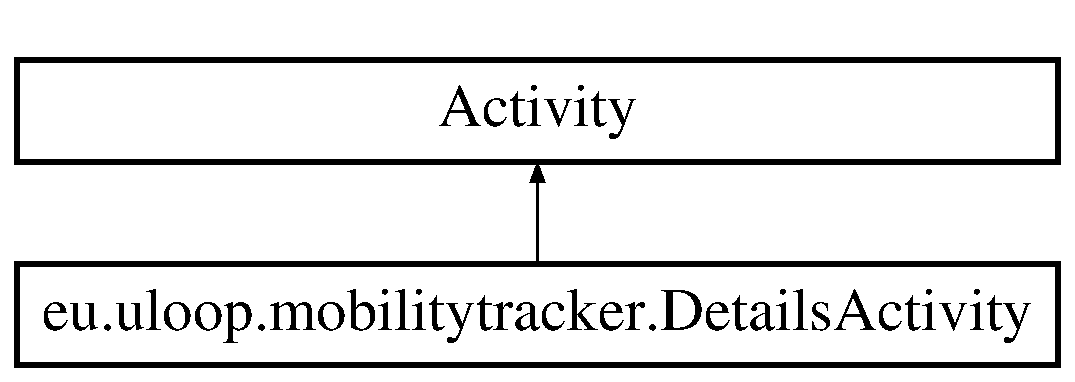
\includegraphics[height=2.000000cm]{classeu_1_1uloop_1_1mobilitytracker_1_1DetailsActivity}
\end{center}
\end{figure}
\subsection*{Protected Member Functions}
\begin{DoxyCompactItemize}
\item 
void \hyperlink{classeu_1_1uloop_1_1mobilitytracker_1_1DetailsActivity_a0b75bac6b06b08a85c9879b820c59ec7}{on\+Create} (Bundle saved\+Instance\+State)
\item 
void \hyperlink{classeu_1_1uloop_1_1mobilitytracker_1_1DetailsActivity_a1a3a01408a7a632c43f2ea12f14c66de}{on\+Start} ()
\item 
void \hyperlink{classeu_1_1uloop_1_1mobilitytracker_1_1DetailsActivity_a440ff757e67eef94d6da34a599c04a96}{on\+Stop} ()
\item 
void \hyperlink{classeu_1_1uloop_1_1mobilitytracker_1_1DetailsActivity_a9c69a0a1329b2ac37a7d86bd344bd86c}{on\+Destroy} ()
\end{DoxyCompactItemize}


\subsection{Detailed Description}
This class provides an activity that shows detailed information of a given A\+P.

\begin{DoxyAuthor}{Author}
Jonnahtan Saltarin (U\+L\+H\+T) 

Rute Sofia (U\+L\+H\+T) 

Christian da Silva Pereira (U\+L\+H\+T) 

Luis Amaral Lopes (U\+L\+H\+T)
\end{DoxyAuthor}
\begin{DoxyVersion}{Version}
3.\+0 
\end{DoxyVersion}


\subsection{Member Function Documentation}
\hypertarget{classeu_1_1uloop_1_1mobilitytracker_1_1DetailsActivity_a0b75bac6b06b08a85c9879b820c59ec7}{\index{eu\+::uloop\+::mobilitytracker\+::\+Details\+Activity@{eu\+::uloop\+::mobilitytracker\+::\+Details\+Activity}!on\+Create@{on\+Create}}
\index{on\+Create@{on\+Create}!eu\+::uloop\+::mobilitytracker\+::\+Details\+Activity@{eu\+::uloop\+::mobilitytracker\+::\+Details\+Activity}}
\subsubsection[{on\+Create}]{\setlength{\rightskip}{0pt plus 5cm}void eu.\+uloop.\+mobilitytracker.\+Details\+Activity.\+on\+Create (
\begin{DoxyParamCaption}
\item[{Bundle}]{saved\+Instance\+State}
\end{DoxyParamCaption}
)\hspace{0.3cm}{\ttfamily [protected]}}}\label{classeu_1_1uloop_1_1mobilitytracker_1_1DetailsActivity_a0b75bac6b06b08a85c9879b820c59ec7}
\hypertarget{classeu_1_1uloop_1_1mobilitytracker_1_1DetailsActivity_a9c69a0a1329b2ac37a7d86bd344bd86c}{\index{eu\+::uloop\+::mobilitytracker\+::\+Details\+Activity@{eu\+::uloop\+::mobilitytracker\+::\+Details\+Activity}!on\+Destroy@{on\+Destroy}}
\index{on\+Destroy@{on\+Destroy}!eu\+::uloop\+::mobilitytracker\+::\+Details\+Activity@{eu\+::uloop\+::mobilitytracker\+::\+Details\+Activity}}
\subsubsection[{on\+Destroy}]{\setlength{\rightskip}{0pt plus 5cm}void eu.\+uloop.\+mobilitytracker.\+Details\+Activity.\+on\+Destroy (
\begin{DoxyParamCaption}
{}
\end{DoxyParamCaption}
)\hspace{0.3cm}{\ttfamily [protected]}}}\label{classeu_1_1uloop_1_1mobilitytracker_1_1DetailsActivity_a9c69a0a1329b2ac37a7d86bd344bd86c}
\hypertarget{classeu_1_1uloop_1_1mobilitytracker_1_1DetailsActivity_a1a3a01408a7a632c43f2ea12f14c66de}{\index{eu\+::uloop\+::mobilitytracker\+::\+Details\+Activity@{eu\+::uloop\+::mobilitytracker\+::\+Details\+Activity}!on\+Start@{on\+Start}}
\index{on\+Start@{on\+Start}!eu\+::uloop\+::mobilitytracker\+::\+Details\+Activity@{eu\+::uloop\+::mobilitytracker\+::\+Details\+Activity}}
\subsubsection[{on\+Start}]{\setlength{\rightskip}{0pt plus 5cm}void eu.\+uloop.\+mobilitytracker.\+Details\+Activity.\+on\+Start (
\begin{DoxyParamCaption}
{}
\end{DoxyParamCaption}
)\hspace{0.3cm}{\ttfamily [protected]}}}\label{classeu_1_1uloop_1_1mobilitytracker_1_1DetailsActivity_a1a3a01408a7a632c43f2ea12f14c66de}
\hypertarget{classeu_1_1uloop_1_1mobilitytracker_1_1DetailsActivity_a440ff757e67eef94d6da34a599c04a96}{\index{eu\+::uloop\+::mobilitytracker\+::\+Details\+Activity@{eu\+::uloop\+::mobilitytracker\+::\+Details\+Activity}!on\+Stop@{on\+Stop}}
\index{on\+Stop@{on\+Stop}!eu\+::uloop\+::mobilitytracker\+::\+Details\+Activity@{eu\+::uloop\+::mobilitytracker\+::\+Details\+Activity}}
\subsubsection[{on\+Stop}]{\setlength{\rightskip}{0pt plus 5cm}void eu.\+uloop.\+mobilitytracker.\+Details\+Activity.\+on\+Stop (
\begin{DoxyParamCaption}
{}
\end{DoxyParamCaption}
)\hspace{0.3cm}{\ttfamily [protected]}}}\label{classeu_1_1uloop_1_1mobilitytracker_1_1DetailsActivity_a440ff757e67eef94d6da34a599c04a96}


The documentation for this class was generated from the following file\+:\begin{DoxyCompactItemize}
\item 
src/eu/uloop/mobilitytracker/\hyperlink{DetailsActivity_8java}{Details\+Activity.\+java}\end{DoxyCompactItemize}

\hypertarget{interfaceeu_1_1uloop_1_1messages_1_1UloopMessages_1_1EnoughResourcesCACReplyOrBuilder}{\section{eu.\+uloop.\+messages.\+Uloop\+Messages.\+Enough\+Resources\+C\+A\+C\+Reply\+Or\+Builder Interface Reference}
\label{interfaceeu_1_1uloop_1_1messages_1_1UloopMessages_1_1EnoughResourcesCACReplyOrBuilder}\index{eu.\+uloop.\+messages.\+Uloop\+Messages.\+Enough\+Resources\+C\+A\+C\+Reply\+Or\+Builder@{eu.\+uloop.\+messages.\+Uloop\+Messages.\+Enough\+Resources\+C\+A\+C\+Reply\+Or\+Builder}}
}
Inheritance diagram for eu.\+uloop.\+messages.\+Uloop\+Messages.\+Enough\+Resources\+C\+A\+C\+Reply\+Or\+Builder\+:\begin{figure}[H]
\begin{center}
\leavevmode
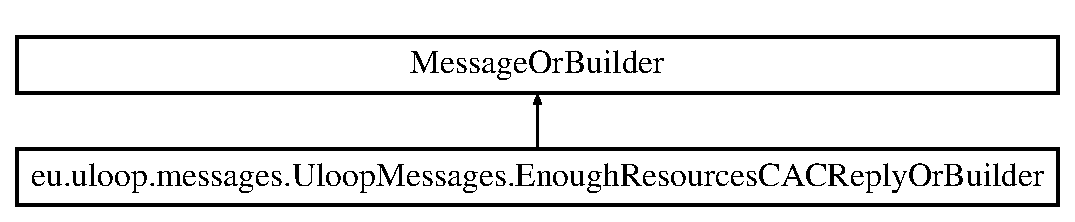
\includegraphics[height=2.000000cm]{interfaceeu_1_1uloop_1_1messages_1_1UloopMessages_1_1EnoughResourcesCACReplyOrBuilder}
\end{center}
\end{figure}
\subsection*{Public Member Functions}
\begin{DoxyCompactItemize}
\item 
boolean \hyperlink{interfaceeu_1_1uloop_1_1messages_1_1UloopMessages_1_1EnoughResourcesCACReplyOrBuilder_a65bdb4101a40652cea28e9b73d9980cb}{has\+Cryptoid} ()
\item 
com.\+google.\+protobuf.\+Byte\+String \hyperlink{interfaceeu_1_1uloop_1_1messages_1_1UloopMessages_1_1EnoughResourcesCACReplyOrBuilder_a4f76439ceffbcd6ba2a1bb5fe94f597d}{get\+Cryptoid} ()
\item 
boolean \hyperlink{interfaceeu_1_1uloop_1_1messages_1_1UloopMessages_1_1EnoughResourcesCACReplyOrBuilder_a7889ec7d12caede1d8d5a0d72f59b111}{has\+Token} ()
\item 
double \hyperlink{interfaceeu_1_1uloop_1_1messages_1_1UloopMessages_1_1EnoughResourcesCACReplyOrBuilder_a4b92ba29b9bd907521fa58152bdfd875}{get\+Token} ()
\item 
boolean \hyperlink{interfaceeu_1_1uloop_1_1messages_1_1UloopMessages_1_1EnoughResourcesCACReplyOrBuilder_a67bc890403e0405914392d7deefb60a2}{has\+Enough} ()
\item 
boolean \hyperlink{interfaceeu_1_1uloop_1_1messages_1_1UloopMessages_1_1EnoughResourcesCACReplyOrBuilder_af75fa7e695738173b3403f510354299f}{get\+Enough} ()
\end{DoxyCompactItemize}


\subsection{Member Function Documentation}
\hypertarget{interfaceeu_1_1uloop_1_1messages_1_1UloopMessages_1_1EnoughResourcesCACReplyOrBuilder_a4f76439ceffbcd6ba2a1bb5fe94f597d}{\index{eu\+::uloop\+::messages\+::\+Uloop\+Messages\+::\+Enough\+Resources\+C\+A\+C\+Reply\+Or\+Builder@{eu\+::uloop\+::messages\+::\+Uloop\+Messages\+::\+Enough\+Resources\+C\+A\+C\+Reply\+Or\+Builder}!get\+Cryptoid@{get\+Cryptoid}}
\index{get\+Cryptoid@{get\+Cryptoid}!eu\+::uloop\+::messages\+::\+Uloop\+Messages\+::\+Enough\+Resources\+C\+A\+C\+Reply\+Or\+Builder@{eu\+::uloop\+::messages\+::\+Uloop\+Messages\+::\+Enough\+Resources\+C\+A\+C\+Reply\+Or\+Builder}}
\subsubsection[{get\+Cryptoid}]{\setlength{\rightskip}{0pt plus 5cm}com.\+google.\+protobuf.\+Byte\+String eu.\+uloop.\+messages.\+Uloop\+Messages.\+Enough\+Resources\+C\+A\+C\+Reply\+Or\+Builder.\+get\+Cryptoid (
\begin{DoxyParamCaption}
{}
\end{DoxyParamCaption}
)}}\label{interfaceeu_1_1uloop_1_1messages_1_1UloopMessages_1_1EnoughResourcesCACReplyOrBuilder_a4f76439ceffbcd6ba2a1bb5fe94f597d}
\hypertarget{interfaceeu_1_1uloop_1_1messages_1_1UloopMessages_1_1EnoughResourcesCACReplyOrBuilder_af75fa7e695738173b3403f510354299f}{\index{eu\+::uloop\+::messages\+::\+Uloop\+Messages\+::\+Enough\+Resources\+C\+A\+C\+Reply\+Or\+Builder@{eu\+::uloop\+::messages\+::\+Uloop\+Messages\+::\+Enough\+Resources\+C\+A\+C\+Reply\+Or\+Builder}!get\+Enough@{get\+Enough}}
\index{get\+Enough@{get\+Enough}!eu\+::uloop\+::messages\+::\+Uloop\+Messages\+::\+Enough\+Resources\+C\+A\+C\+Reply\+Or\+Builder@{eu\+::uloop\+::messages\+::\+Uloop\+Messages\+::\+Enough\+Resources\+C\+A\+C\+Reply\+Or\+Builder}}
\subsubsection[{get\+Enough}]{\setlength{\rightskip}{0pt plus 5cm}boolean eu.\+uloop.\+messages.\+Uloop\+Messages.\+Enough\+Resources\+C\+A\+C\+Reply\+Or\+Builder.\+get\+Enough (
\begin{DoxyParamCaption}
{}
\end{DoxyParamCaption}
)}}\label{interfaceeu_1_1uloop_1_1messages_1_1UloopMessages_1_1EnoughResourcesCACReplyOrBuilder_af75fa7e695738173b3403f510354299f}
\hypertarget{interfaceeu_1_1uloop_1_1messages_1_1UloopMessages_1_1EnoughResourcesCACReplyOrBuilder_a4b92ba29b9bd907521fa58152bdfd875}{\index{eu\+::uloop\+::messages\+::\+Uloop\+Messages\+::\+Enough\+Resources\+C\+A\+C\+Reply\+Or\+Builder@{eu\+::uloop\+::messages\+::\+Uloop\+Messages\+::\+Enough\+Resources\+C\+A\+C\+Reply\+Or\+Builder}!get\+Token@{get\+Token}}
\index{get\+Token@{get\+Token}!eu\+::uloop\+::messages\+::\+Uloop\+Messages\+::\+Enough\+Resources\+C\+A\+C\+Reply\+Or\+Builder@{eu\+::uloop\+::messages\+::\+Uloop\+Messages\+::\+Enough\+Resources\+C\+A\+C\+Reply\+Or\+Builder}}
\subsubsection[{get\+Token}]{\setlength{\rightskip}{0pt plus 5cm}double eu.\+uloop.\+messages.\+Uloop\+Messages.\+Enough\+Resources\+C\+A\+C\+Reply\+Or\+Builder.\+get\+Token (
\begin{DoxyParamCaption}
{}
\end{DoxyParamCaption}
)}}\label{interfaceeu_1_1uloop_1_1messages_1_1UloopMessages_1_1EnoughResourcesCACReplyOrBuilder_a4b92ba29b9bd907521fa58152bdfd875}
\hypertarget{interfaceeu_1_1uloop_1_1messages_1_1UloopMessages_1_1EnoughResourcesCACReplyOrBuilder_a65bdb4101a40652cea28e9b73d9980cb}{\index{eu\+::uloop\+::messages\+::\+Uloop\+Messages\+::\+Enough\+Resources\+C\+A\+C\+Reply\+Or\+Builder@{eu\+::uloop\+::messages\+::\+Uloop\+Messages\+::\+Enough\+Resources\+C\+A\+C\+Reply\+Or\+Builder}!has\+Cryptoid@{has\+Cryptoid}}
\index{has\+Cryptoid@{has\+Cryptoid}!eu\+::uloop\+::messages\+::\+Uloop\+Messages\+::\+Enough\+Resources\+C\+A\+C\+Reply\+Or\+Builder@{eu\+::uloop\+::messages\+::\+Uloop\+Messages\+::\+Enough\+Resources\+C\+A\+C\+Reply\+Or\+Builder}}
\subsubsection[{has\+Cryptoid}]{\setlength{\rightskip}{0pt plus 5cm}boolean eu.\+uloop.\+messages.\+Uloop\+Messages.\+Enough\+Resources\+C\+A\+C\+Reply\+Or\+Builder.\+has\+Cryptoid (
\begin{DoxyParamCaption}
{}
\end{DoxyParamCaption}
)}}\label{interfaceeu_1_1uloop_1_1messages_1_1UloopMessages_1_1EnoughResourcesCACReplyOrBuilder_a65bdb4101a40652cea28e9b73d9980cb}
\hypertarget{interfaceeu_1_1uloop_1_1messages_1_1UloopMessages_1_1EnoughResourcesCACReplyOrBuilder_a67bc890403e0405914392d7deefb60a2}{\index{eu\+::uloop\+::messages\+::\+Uloop\+Messages\+::\+Enough\+Resources\+C\+A\+C\+Reply\+Or\+Builder@{eu\+::uloop\+::messages\+::\+Uloop\+Messages\+::\+Enough\+Resources\+C\+A\+C\+Reply\+Or\+Builder}!has\+Enough@{has\+Enough}}
\index{has\+Enough@{has\+Enough}!eu\+::uloop\+::messages\+::\+Uloop\+Messages\+::\+Enough\+Resources\+C\+A\+C\+Reply\+Or\+Builder@{eu\+::uloop\+::messages\+::\+Uloop\+Messages\+::\+Enough\+Resources\+C\+A\+C\+Reply\+Or\+Builder}}
\subsubsection[{has\+Enough}]{\setlength{\rightskip}{0pt plus 5cm}boolean eu.\+uloop.\+messages.\+Uloop\+Messages.\+Enough\+Resources\+C\+A\+C\+Reply\+Or\+Builder.\+has\+Enough (
\begin{DoxyParamCaption}
{}
\end{DoxyParamCaption}
)}}\label{interfaceeu_1_1uloop_1_1messages_1_1UloopMessages_1_1EnoughResourcesCACReplyOrBuilder_a67bc890403e0405914392d7deefb60a2}
\hypertarget{interfaceeu_1_1uloop_1_1messages_1_1UloopMessages_1_1EnoughResourcesCACReplyOrBuilder_a7889ec7d12caede1d8d5a0d72f59b111}{\index{eu\+::uloop\+::messages\+::\+Uloop\+Messages\+::\+Enough\+Resources\+C\+A\+C\+Reply\+Or\+Builder@{eu\+::uloop\+::messages\+::\+Uloop\+Messages\+::\+Enough\+Resources\+C\+A\+C\+Reply\+Or\+Builder}!has\+Token@{has\+Token}}
\index{has\+Token@{has\+Token}!eu\+::uloop\+::messages\+::\+Uloop\+Messages\+::\+Enough\+Resources\+C\+A\+C\+Reply\+Or\+Builder@{eu\+::uloop\+::messages\+::\+Uloop\+Messages\+::\+Enough\+Resources\+C\+A\+C\+Reply\+Or\+Builder}}
\subsubsection[{has\+Token}]{\setlength{\rightskip}{0pt plus 5cm}boolean eu.\+uloop.\+messages.\+Uloop\+Messages.\+Enough\+Resources\+C\+A\+C\+Reply\+Or\+Builder.\+has\+Token (
\begin{DoxyParamCaption}
{}
\end{DoxyParamCaption}
)}}\label{interfaceeu_1_1uloop_1_1messages_1_1UloopMessages_1_1EnoughResourcesCACReplyOrBuilder_a7889ec7d12caede1d8d5a0d72f59b111}


The documentation for this interface was generated from the following file\+:\begin{DoxyCompactItemize}
\item 
src/eu/uloop/messages/\hyperlink{UloopMessages_8java}{Uloop\+Messages.\+java}\end{DoxyCompactItemize}

\hypertarget{interfaceeu_1_1uloop_1_1messages_1_1UloopMessages_1_1EnoughResourcesMessageReplyOrBuilder}{\section{eu.\+uloop.\+messages.\+Uloop\+Messages.\+Enough\+Resources\+Message\+Reply\+Or\+Builder Interface Reference}
\label{interfaceeu_1_1uloop_1_1messages_1_1UloopMessages_1_1EnoughResourcesMessageReplyOrBuilder}\index{eu.\+uloop.\+messages.\+Uloop\+Messages.\+Enough\+Resources\+Message\+Reply\+Or\+Builder@{eu.\+uloop.\+messages.\+Uloop\+Messages.\+Enough\+Resources\+Message\+Reply\+Or\+Builder}}
}
Inheritance diagram for eu.\+uloop.\+messages.\+Uloop\+Messages.\+Enough\+Resources\+Message\+Reply\+Or\+Builder\+:\begin{figure}[H]
\begin{center}
\leavevmode
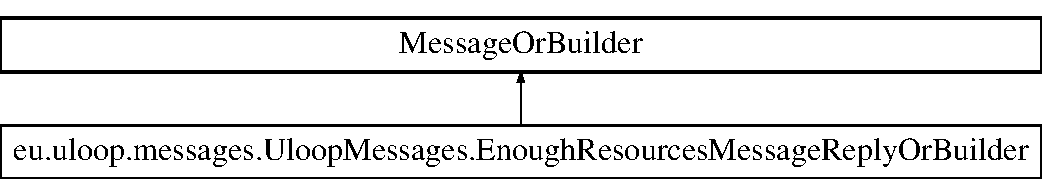
\includegraphics[height=2.000000cm]{interfaceeu_1_1uloop_1_1messages_1_1UloopMessages_1_1EnoughResourcesMessageReplyOrBuilder}
\end{center}
\end{figure}
\subsection*{Public Member Functions}
\begin{DoxyCompactItemize}
\item 
boolean \hyperlink{interfaceeu_1_1uloop_1_1messages_1_1UloopMessages_1_1EnoughResourcesMessageReplyOrBuilder_a980a1af33fe496b4ef122b0233d82052}{has\+Res} ()
\item 
boolean \hyperlink{interfaceeu_1_1uloop_1_1messages_1_1UloopMessages_1_1EnoughResourcesMessageReplyOrBuilder_a7720d29323e2998eb7a72bb40dd876dc}{get\+Res} ()
\end{DoxyCompactItemize}


\subsection{Member Function Documentation}
\hypertarget{interfaceeu_1_1uloop_1_1messages_1_1UloopMessages_1_1EnoughResourcesMessageReplyOrBuilder_a7720d29323e2998eb7a72bb40dd876dc}{\index{eu\+::uloop\+::messages\+::\+Uloop\+Messages\+::\+Enough\+Resources\+Message\+Reply\+Or\+Builder@{eu\+::uloop\+::messages\+::\+Uloop\+Messages\+::\+Enough\+Resources\+Message\+Reply\+Or\+Builder}!get\+Res@{get\+Res}}
\index{get\+Res@{get\+Res}!eu\+::uloop\+::messages\+::\+Uloop\+Messages\+::\+Enough\+Resources\+Message\+Reply\+Or\+Builder@{eu\+::uloop\+::messages\+::\+Uloop\+Messages\+::\+Enough\+Resources\+Message\+Reply\+Or\+Builder}}
\subsubsection[{get\+Res}]{\setlength{\rightskip}{0pt plus 5cm}boolean eu.\+uloop.\+messages.\+Uloop\+Messages.\+Enough\+Resources\+Message\+Reply\+Or\+Builder.\+get\+Res (
\begin{DoxyParamCaption}
{}
\end{DoxyParamCaption}
)}}\label{interfaceeu_1_1uloop_1_1messages_1_1UloopMessages_1_1EnoughResourcesMessageReplyOrBuilder_a7720d29323e2998eb7a72bb40dd876dc}
\hypertarget{interfaceeu_1_1uloop_1_1messages_1_1UloopMessages_1_1EnoughResourcesMessageReplyOrBuilder_a980a1af33fe496b4ef122b0233d82052}{\index{eu\+::uloop\+::messages\+::\+Uloop\+Messages\+::\+Enough\+Resources\+Message\+Reply\+Or\+Builder@{eu\+::uloop\+::messages\+::\+Uloop\+Messages\+::\+Enough\+Resources\+Message\+Reply\+Or\+Builder}!has\+Res@{has\+Res}}
\index{has\+Res@{has\+Res}!eu\+::uloop\+::messages\+::\+Uloop\+Messages\+::\+Enough\+Resources\+Message\+Reply\+Or\+Builder@{eu\+::uloop\+::messages\+::\+Uloop\+Messages\+::\+Enough\+Resources\+Message\+Reply\+Or\+Builder}}
\subsubsection[{has\+Res}]{\setlength{\rightskip}{0pt plus 5cm}boolean eu.\+uloop.\+messages.\+Uloop\+Messages.\+Enough\+Resources\+Message\+Reply\+Or\+Builder.\+has\+Res (
\begin{DoxyParamCaption}
{}
\end{DoxyParamCaption}
)}}\label{interfaceeu_1_1uloop_1_1messages_1_1UloopMessages_1_1EnoughResourcesMessageReplyOrBuilder_a980a1af33fe496b4ef122b0233d82052}


The documentation for this interface was generated from the following file\+:\begin{DoxyCompactItemize}
\item 
src/eu/uloop/messages/\hyperlink{UloopMessages_8java}{Uloop\+Messages.\+java}\end{DoxyCompactItemize}

\hypertarget{interfaceeu_1_1uloop_1_1messages_1_1UloopMessages_1_1EnoughResourcesMessageRequestOrBuilder}{\section{eu.\+uloop.\+messages.\+Uloop\+Messages.\+Enough\+Resources\+Message\+Request\+Or\+Builder Interface Reference}
\label{interfaceeu_1_1uloop_1_1messages_1_1UloopMessages_1_1EnoughResourcesMessageRequestOrBuilder}\index{eu.\+uloop.\+messages.\+Uloop\+Messages.\+Enough\+Resources\+Message\+Request\+Or\+Builder@{eu.\+uloop.\+messages.\+Uloop\+Messages.\+Enough\+Resources\+Message\+Request\+Or\+Builder}}
}
Inheritance diagram for eu.\+uloop.\+messages.\+Uloop\+Messages.\+Enough\+Resources\+Message\+Request\+Or\+Builder\+:\begin{figure}[H]
\begin{center}
\leavevmode
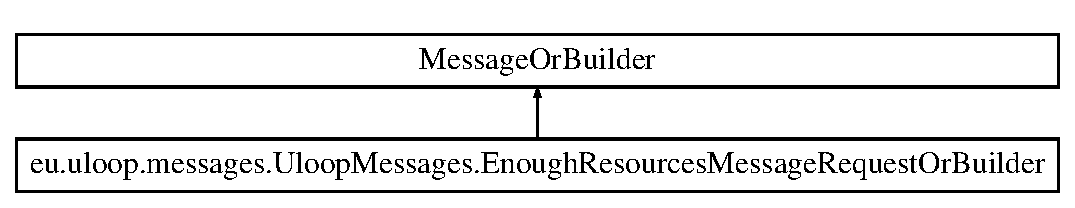
\includegraphics[height=2.000000cm]{interfaceeu_1_1uloop_1_1messages_1_1UloopMessages_1_1EnoughResourcesMessageRequestOrBuilder}
\end{center}
\end{figure}
\subsection*{Public Member Functions}
\begin{DoxyCompactItemize}
\item 
boolean \hyperlink{interfaceeu_1_1uloop_1_1messages_1_1UloopMessages_1_1EnoughResourcesMessageRequestOrBuilder_acb6b122d250a9d33b1719cf09c503a92}{has\+Cryptoid} ()
\item 
com.\+google.\+protobuf.\+Byte\+String \hyperlink{interfaceeu_1_1uloop_1_1messages_1_1UloopMessages_1_1EnoughResourcesMessageRequestOrBuilder_a4dab493ebc532d67379d4effa1571948}{get\+Cryptoid} ()
\item 
boolean \hyperlink{interfaceeu_1_1uloop_1_1messages_1_1UloopMessages_1_1EnoughResourcesMessageRequestOrBuilder_ad6a44338faeecfb2e0d8136ceb58d133}{has\+Token} ()
\item 
double \hyperlink{interfaceeu_1_1uloop_1_1messages_1_1UloopMessages_1_1EnoughResourcesMessageRequestOrBuilder_a79f2612a20e1d83e8e1ae0702435e2a0}{get\+Token} ()
\item 
boolean \hyperlink{interfaceeu_1_1uloop_1_1messages_1_1UloopMessages_1_1EnoughResourcesMessageRequestOrBuilder_affc52875e965cf2529453ff79f8f9a69}{has\+Macaddress} ()
\item 
com.\+google.\+protobuf.\+Byte\+String \hyperlink{interfaceeu_1_1uloop_1_1messages_1_1UloopMessages_1_1EnoughResourcesMessageRequestOrBuilder_aa25de85e180eb723b9ec337c841f64f9}{get\+Macaddress} ()
\end{DoxyCompactItemize}


\subsection{Member Function Documentation}
\hypertarget{interfaceeu_1_1uloop_1_1messages_1_1UloopMessages_1_1EnoughResourcesMessageRequestOrBuilder_a4dab493ebc532d67379d4effa1571948}{\index{eu\+::uloop\+::messages\+::\+Uloop\+Messages\+::\+Enough\+Resources\+Message\+Request\+Or\+Builder@{eu\+::uloop\+::messages\+::\+Uloop\+Messages\+::\+Enough\+Resources\+Message\+Request\+Or\+Builder}!get\+Cryptoid@{get\+Cryptoid}}
\index{get\+Cryptoid@{get\+Cryptoid}!eu\+::uloop\+::messages\+::\+Uloop\+Messages\+::\+Enough\+Resources\+Message\+Request\+Or\+Builder@{eu\+::uloop\+::messages\+::\+Uloop\+Messages\+::\+Enough\+Resources\+Message\+Request\+Or\+Builder}}
\subsubsection[{get\+Cryptoid}]{\setlength{\rightskip}{0pt plus 5cm}com.\+google.\+protobuf.\+Byte\+String eu.\+uloop.\+messages.\+Uloop\+Messages.\+Enough\+Resources\+Message\+Request\+Or\+Builder.\+get\+Cryptoid (
\begin{DoxyParamCaption}
{}
\end{DoxyParamCaption}
)}}\label{interfaceeu_1_1uloop_1_1messages_1_1UloopMessages_1_1EnoughResourcesMessageRequestOrBuilder_a4dab493ebc532d67379d4effa1571948}
\hypertarget{interfaceeu_1_1uloop_1_1messages_1_1UloopMessages_1_1EnoughResourcesMessageRequestOrBuilder_aa25de85e180eb723b9ec337c841f64f9}{\index{eu\+::uloop\+::messages\+::\+Uloop\+Messages\+::\+Enough\+Resources\+Message\+Request\+Or\+Builder@{eu\+::uloop\+::messages\+::\+Uloop\+Messages\+::\+Enough\+Resources\+Message\+Request\+Or\+Builder}!get\+Macaddress@{get\+Macaddress}}
\index{get\+Macaddress@{get\+Macaddress}!eu\+::uloop\+::messages\+::\+Uloop\+Messages\+::\+Enough\+Resources\+Message\+Request\+Or\+Builder@{eu\+::uloop\+::messages\+::\+Uloop\+Messages\+::\+Enough\+Resources\+Message\+Request\+Or\+Builder}}
\subsubsection[{get\+Macaddress}]{\setlength{\rightskip}{0pt plus 5cm}com.\+google.\+protobuf.\+Byte\+String eu.\+uloop.\+messages.\+Uloop\+Messages.\+Enough\+Resources\+Message\+Request\+Or\+Builder.\+get\+Macaddress (
\begin{DoxyParamCaption}
{}
\end{DoxyParamCaption}
)}}\label{interfaceeu_1_1uloop_1_1messages_1_1UloopMessages_1_1EnoughResourcesMessageRequestOrBuilder_aa25de85e180eb723b9ec337c841f64f9}
\hypertarget{interfaceeu_1_1uloop_1_1messages_1_1UloopMessages_1_1EnoughResourcesMessageRequestOrBuilder_a79f2612a20e1d83e8e1ae0702435e2a0}{\index{eu\+::uloop\+::messages\+::\+Uloop\+Messages\+::\+Enough\+Resources\+Message\+Request\+Or\+Builder@{eu\+::uloop\+::messages\+::\+Uloop\+Messages\+::\+Enough\+Resources\+Message\+Request\+Or\+Builder}!get\+Token@{get\+Token}}
\index{get\+Token@{get\+Token}!eu\+::uloop\+::messages\+::\+Uloop\+Messages\+::\+Enough\+Resources\+Message\+Request\+Or\+Builder@{eu\+::uloop\+::messages\+::\+Uloop\+Messages\+::\+Enough\+Resources\+Message\+Request\+Or\+Builder}}
\subsubsection[{get\+Token}]{\setlength{\rightskip}{0pt plus 5cm}double eu.\+uloop.\+messages.\+Uloop\+Messages.\+Enough\+Resources\+Message\+Request\+Or\+Builder.\+get\+Token (
\begin{DoxyParamCaption}
{}
\end{DoxyParamCaption}
)}}\label{interfaceeu_1_1uloop_1_1messages_1_1UloopMessages_1_1EnoughResourcesMessageRequestOrBuilder_a79f2612a20e1d83e8e1ae0702435e2a0}
\hypertarget{interfaceeu_1_1uloop_1_1messages_1_1UloopMessages_1_1EnoughResourcesMessageRequestOrBuilder_acb6b122d250a9d33b1719cf09c503a92}{\index{eu\+::uloop\+::messages\+::\+Uloop\+Messages\+::\+Enough\+Resources\+Message\+Request\+Or\+Builder@{eu\+::uloop\+::messages\+::\+Uloop\+Messages\+::\+Enough\+Resources\+Message\+Request\+Or\+Builder}!has\+Cryptoid@{has\+Cryptoid}}
\index{has\+Cryptoid@{has\+Cryptoid}!eu\+::uloop\+::messages\+::\+Uloop\+Messages\+::\+Enough\+Resources\+Message\+Request\+Or\+Builder@{eu\+::uloop\+::messages\+::\+Uloop\+Messages\+::\+Enough\+Resources\+Message\+Request\+Or\+Builder}}
\subsubsection[{has\+Cryptoid}]{\setlength{\rightskip}{0pt plus 5cm}boolean eu.\+uloop.\+messages.\+Uloop\+Messages.\+Enough\+Resources\+Message\+Request\+Or\+Builder.\+has\+Cryptoid (
\begin{DoxyParamCaption}
{}
\end{DoxyParamCaption}
)}}\label{interfaceeu_1_1uloop_1_1messages_1_1UloopMessages_1_1EnoughResourcesMessageRequestOrBuilder_acb6b122d250a9d33b1719cf09c503a92}
\hypertarget{interfaceeu_1_1uloop_1_1messages_1_1UloopMessages_1_1EnoughResourcesMessageRequestOrBuilder_affc52875e965cf2529453ff79f8f9a69}{\index{eu\+::uloop\+::messages\+::\+Uloop\+Messages\+::\+Enough\+Resources\+Message\+Request\+Or\+Builder@{eu\+::uloop\+::messages\+::\+Uloop\+Messages\+::\+Enough\+Resources\+Message\+Request\+Or\+Builder}!has\+Macaddress@{has\+Macaddress}}
\index{has\+Macaddress@{has\+Macaddress}!eu\+::uloop\+::messages\+::\+Uloop\+Messages\+::\+Enough\+Resources\+Message\+Request\+Or\+Builder@{eu\+::uloop\+::messages\+::\+Uloop\+Messages\+::\+Enough\+Resources\+Message\+Request\+Or\+Builder}}
\subsubsection[{has\+Macaddress}]{\setlength{\rightskip}{0pt plus 5cm}boolean eu.\+uloop.\+messages.\+Uloop\+Messages.\+Enough\+Resources\+Message\+Request\+Or\+Builder.\+has\+Macaddress (
\begin{DoxyParamCaption}
{}
\end{DoxyParamCaption}
)}}\label{interfaceeu_1_1uloop_1_1messages_1_1UloopMessages_1_1EnoughResourcesMessageRequestOrBuilder_affc52875e965cf2529453ff79f8f9a69}
\hypertarget{interfaceeu_1_1uloop_1_1messages_1_1UloopMessages_1_1EnoughResourcesMessageRequestOrBuilder_ad6a44338faeecfb2e0d8136ceb58d133}{\index{eu\+::uloop\+::messages\+::\+Uloop\+Messages\+::\+Enough\+Resources\+Message\+Request\+Or\+Builder@{eu\+::uloop\+::messages\+::\+Uloop\+Messages\+::\+Enough\+Resources\+Message\+Request\+Or\+Builder}!has\+Token@{has\+Token}}
\index{has\+Token@{has\+Token}!eu\+::uloop\+::messages\+::\+Uloop\+Messages\+::\+Enough\+Resources\+Message\+Request\+Or\+Builder@{eu\+::uloop\+::messages\+::\+Uloop\+Messages\+::\+Enough\+Resources\+Message\+Request\+Or\+Builder}}
\subsubsection[{has\+Token}]{\setlength{\rightskip}{0pt plus 5cm}boolean eu.\+uloop.\+messages.\+Uloop\+Messages.\+Enough\+Resources\+Message\+Request\+Or\+Builder.\+has\+Token (
\begin{DoxyParamCaption}
{}
\end{DoxyParamCaption}
)}}\label{interfaceeu_1_1uloop_1_1messages_1_1UloopMessages_1_1EnoughResourcesMessageRequestOrBuilder_ad6a44338faeecfb2e0d8136ceb58d133}


The documentation for this interface was generated from the following file\+:\begin{DoxyCompactItemize}
\item 
src/eu/uloop/messages/\hyperlink{UloopMessages_8java}{Uloop\+Messages.\+java}\end{DoxyCompactItemize}

\hypertarget{classeu_1_1uloop_1_1mobilitytracker_1_1MTrackerService_1_1LocalBinder}{\section{eu.\+uloop.\+mobilitytracker.\+M\+Tracker\+Service.\+Local\+Binder Class Reference}
\label{classeu_1_1uloop_1_1mobilitytracker_1_1MTrackerService_1_1LocalBinder}\index{eu.\+uloop.\+mobilitytracker.\+M\+Tracker\+Service.\+Local\+Binder@{eu.\+uloop.\+mobilitytracker.\+M\+Tracker\+Service.\+Local\+Binder}}
}
Inheritance diagram for eu.\+uloop.\+mobilitytracker.\+M\+Tracker\+Service.\+Local\+Binder\+:\begin{figure}[H]
\begin{center}
\leavevmode
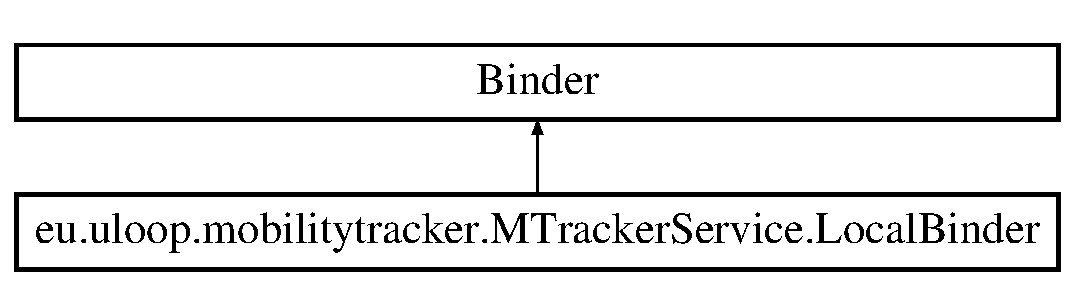
\includegraphics[height=2.000000cm]{classeu_1_1uloop_1_1mobilitytracker_1_1MTrackerService_1_1LocalBinder}
\end{center}
\end{figure}


The documentation for this class was generated from the following file\+:\begin{DoxyCompactItemize}
\item 
src/eu/uloop/mobilitytracker/\hyperlink{MTrackerService_8java}{M\+Tracker\+Service.\+java}\end{DoxyCompactItemize}

\hypertarget{classlib_1_1api_1_1MessageDigest}{\section{lib.\+api.\+Message\+Digest Class Reference}
\label{classlib_1_1api_1_1MessageDigest}\index{lib.\+api.\+Message\+Digest@{lib.\+api.\+Message\+Digest}}
}
\subsection*{Static Public Member Functions}
\begin{DoxyCompactItemize}
\item 
static byte\mbox{[}$\,$\mbox{]} \hyperlink{classlib_1_1api_1_1MessageDigest_a928030678791a5ea1112d58ed740b956}{hash\+Public\+Key} (Public\+Key pk)
\item 
static byte\mbox{[}$\,$\mbox{]} \hyperlink{classlib_1_1api_1_1MessageDigest_a2b0cabe98c65c8e9f959563c63dbb0df}{hash\+Public\+Key\+M\+A\+C} (Public\+Key pk, byte\mbox{[}$\,$\mbox{]}mac)
\item 
static byte\mbox{[}$\,$\mbox{]} \hyperlink{classlib_1_1api_1_1MessageDigest_a8ae0db81a402dbb0e301b0cf82aa3d71}{hash\+Public\+Key\+M\+A\+C\+Alt} (Public\+Key pk, byte\mbox{[}$\,$\mbox{]}mac)
\item 
static byte\mbox{[}$\,$\mbox{]} \hyperlink{classlib_1_1api_1_1MessageDigest_a2d69c865e045d5a3e58ccec9a9cf28bc}{S\+H\+A256\+Bytes} (byte\mbox{[}$\,$\mbox{]}key)
\end{DoxyCompactItemize}


\subsection{Member Function Documentation}
\hypertarget{classlib_1_1api_1_1MessageDigest_a928030678791a5ea1112d58ed740b956}{\index{lib\+::api\+::\+Message\+Digest@{lib\+::api\+::\+Message\+Digest}!hash\+Public\+Key@{hash\+Public\+Key}}
\index{hash\+Public\+Key@{hash\+Public\+Key}!lib\+::api\+::\+Message\+Digest@{lib\+::api\+::\+Message\+Digest}}
\subsubsection[{hash\+Public\+Key}]{\setlength{\rightskip}{0pt plus 5cm}static byte \mbox{[}$\,$\mbox{]} lib.\+api.\+Message\+Digest.\+hash\+Public\+Key (
\begin{DoxyParamCaption}
\item[{Public\+Key}]{pk}
\end{DoxyParamCaption}
)\hspace{0.3cm}{\ttfamily [static]}}}\label{classlib_1_1api_1_1MessageDigest_a928030678791a5ea1112d58ed740b956}
\hypertarget{classlib_1_1api_1_1MessageDigest_a2b0cabe98c65c8e9f959563c63dbb0df}{\index{lib\+::api\+::\+Message\+Digest@{lib\+::api\+::\+Message\+Digest}!hash\+Public\+Key\+M\+A\+C@{hash\+Public\+Key\+M\+A\+C}}
\index{hash\+Public\+Key\+M\+A\+C@{hash\+Public\+Key\+M\+A\+C}!lib\+::api\+::\+Message\+Digest@{lib\+::api\+::\+Message\+Digest}}
\subsubsection[{hash\+Public\+Key\+M\+A\+C}]{\setlength{\rightskip}{0pt plus 5cm}static byte \mbox{[}$\,$\mbox{]} lib.\+api.\+Message\+Digest.\+hash\+Public\+Key\+M\+A\+C (
\begin{DoxyParamCaption}
\item[{Public\+Key}]{pk, }
\item[{byte\mbox{[}$\,$\mbox{]}}]{mac}
\end{DoxyParamCaption}
)\hspace{0.3cm}{\ttfamily [static]}}}\label{classlib_1_1api_1_1MessageDigest_a2b0cabe98c65c8e9f959563c63dbb0df}
\hypertarget{classlib_1_1api_1_1MessageDigest_a8ae0db81a402dbb0e301b0cf82aa3d71}{\index{lib\+::api\+::\+Message\+Digest@{lib\+::api\+::\+Message\+Digest}!hash\+Public\+Key\+M\+A\+C\+Alt@{hash\+Public\+Key\+M\+A\+C\+Alt}}
\index{hash\+Public\+Key\+M\+A\+C\+Alt@{hash\+Public\+Key\+M\+A\+C\+Alt}!lib\+::api\+::\+Message\+Digest@{lib\+::api\+::\+Message\+Digest}}
\subsubsection[{hash\+Public\+Key\+M\+A\+C\+Alt}]{\setlength{\rightskip}{0pt plus 5cm}static byte \mbox{[}$\,$\mbox{]} lib.\+api.\+Message\+Digest.\+hash\+Public\+Key\+M\+A\+C\+Alt (
\begin{DoxyParamCaption}
\item[{Public\+Key}]{pk, }
\item[{byte\mbox{[}$\,$\mbox{]}}]{mac}
\end{DoxyParamCaption}
)\hspace{0.3cm}{\ttfamily [static]}}}\label{classlib_1_1api_1_1MessageDigest_a8ae0db81a402dbb0e301b0cf82aa3d71}
\hypertarget{classlib_1_1api_1_1MessageDigest_a2d69c865e045d5a3e58ccec9a9cf28bc}{\index{lib\+::api\+::\+Message\+Digest@{lib\+::api\+::\+Message\+Digest}!S\+H\+A256\+Bytes@{S\+H\+A256\+Bytes}}
\index{S\+H\+A256\+Bytes@{S\+H\+A256\+Bytes}!lib\+::api\+::\+Message\+Digest@{lib\+::api\+::\+Message\+Digest}}
\subsubsection[{S\+H\+A256\+Bytes}]{\setlength{\rightskip}{0pt plus 5cm}static byte \mbox{[}$\,$\mbox{]} lib.\+api.\+Message\+Digest.\+S\+H\+A256\+Bytes (
\begin{DoxyParamCaption}
\item[{byte\mbox{[}$\,$\mbox{]}}]{key}
\end{DoxyParamCaption}
)\hspace{0.3cm}{\ttfamily [static]}}}\label{classlib_1_1api_1_1MessageDigest_a2d69c865e045d5a3e58ccec9a9cf28bc}


The documentation for this class was generated from the following file\+:\begin{DoxyCompactItemize}
\item 
src/lib/api/\hyperlink{MessageDigest_8java}{Message\+Digest.\+java}\end{DoxyCompactItemize}

\hypertarget{enumeu_1_1uloop_1_1messages_1_1UloopMessages_1_1MessageType}{\section{eu.\+uloop.\+messages.\+Uloop\+Messages.\+Message\+Type Enum Reference}
\label{enumeu_1_1uloop_1_1messages_1_1UloopMessages_1_1MessageType}\index{eu.\+uloop.\+messages.\+Uloop\+Messages.\+Message\+Type@{eu.\+uloop.\+messages.\+Uloop\+Messages.\+Message\+Type}}
}
Inheritance diagram for eu.\+uloop.\+messages.\+Uloop\+Messages.\+Message\+Type\+:\begin{figure}[H]
\begin{center}
\leavevmode
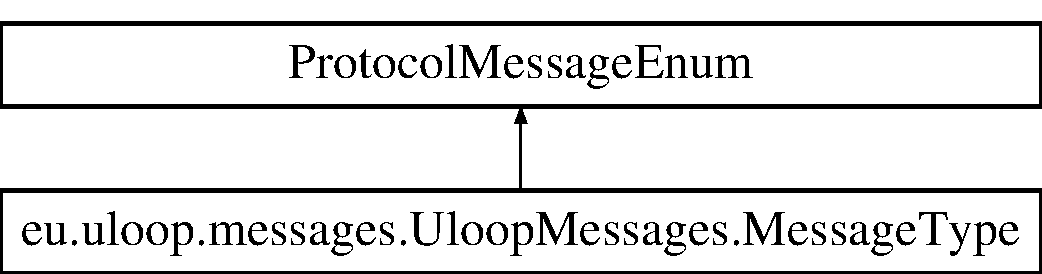
\includegraphics[height=2.000000cm]{enumeu_1_1uloop_1_1messages_1_1UloopMessages_1_1MessageType}
\end{center}
\end{figure}
\subsection*{Public Member Functions}
\begin{DoxyCompactItemize}
\item 
final int \hyperlink{enumeu_1_1uloop_1_1messages_1_1UloopMessages_1_1MessageType_ac1472a5a2060fee965858e15115df937}{get\+Number} ()
\item 
final \\*
com.\+google.\+protobuf.\+Descriptors.\+Enum\+Value\+Descriptor \hyperlink{enumeu_1_1uloop_1_1messages_1_1UloopMessages_1_1MessageType_ae65cf2f08909d256fdaef6403683d190}{get\+Value\+Descriptor} ()
\item 
final \\*
com.\+google.\+protobuf.\+Descriptors.\+Enum\+Descriptor \hyperlink{enumeu_1_1uloop_1_1messages_1_1UloopMessages_1_1MessageType_a1db616c0deb9e389091b6ac7b9e599ae}{get\+Descriptor\+For\+Type} ()
\end{DoxyCompactItemize}
\subsection*{Static Public Member Functions}
\begin{DoxyCompactItemize}
\item 
static \hyperlink{enumeu_1_1uloop_1_1messages_1_1UloopMessages_1_1MessageType}{Message\+Type} \hyperlink{enumeu_1_1uloop_1_1messages_1_1UloopMessages_1_1MessageType_afded6405b021c830067613cea71ad380}{value\+Of} (int \hyperlink{enumeu_1_1uloop_1_1messages_1_1UloopMessages_1_1MessageType_ae860165fa03af44a4a66dba11804a8c4}{value})
\item 
static \\*
com.\+google.\+protobuf.\+Internal.\+Enum\+Lite\+Map\\*
$<$ \hyperlink{enumeu_1_1uloop_1_1messages_1_1UloopMessages_1_1MessageType}{Message\+Type} $>$ \hyperlink{enumeu_1_1uloop_1_1messages_1_1UloopMessages_1_1MessageType_ae0eb3b9a0a81eb3f894b37671c7c0478}{internal\+Get\+Value\+Map} ()
\item 
static final \\*
com.\+google.\+protobuf.\+Descriptors.\+Enum\+Descriptor \hyperlink{enumeu_1_1uloop_1_1messages_1_1UloopMessages_1_1MessageType_af0a1bfd1245af065dfeb691a01a9dc67}{get\+Descriptor} ()
\item 
static \hyperlink{enumeu_1_1uloop_1_1messages_1_1UloopMessages_1_1MessageType}{Message\+Type} \hyperlink{enumeu_1_1uloop_1_1messages_1_1UloopMessages_1_1MessageType_afac766e34825131aa5e741259d1205b5}{value\+Of} (com.\+google.\+protobuf.\+Descriptors.\+Enum\+Value\+Descriptor desc)
\end{DoxyCompactItemize}
\subsection*{Public Attributes}
\begin{DoxyCompactItemize}
\item 
\hyperlink{enumeu_1_1uloop_1_1messages_1_1UloopMessages_1_1MessageType_a17c9f76c79e43ab31e2a5057b192c675}{U\+N\+S\+P\+E\+C} =(0, 0)
\item 
\hyperlink{enumeu_1_1uloop_1_1messages_1_1UloopMessages_1_1MessageType_a3243c417eb643e8d89f0639694af2d52}{T\+R\+U\+S\+T\+\_\+\+M\+E\+S\+S\+A\+G\+E} =(1, 1)
\item 
\hyperlink{enumeu_1_1uloop_1_1messages_1_1UloopMessages_1_1MessageType_af82bbd584b35e878e9f483ddc199ee35}{T\+R\+U\+S\+T\+\_\+\+I\+N\+F\+O\+R\+M\+A\+T\+I\+O\+N\+\_\+\+R\+E\+Q\+U\+E\+S\+T} =(2, 2)
\item 
\hyperlink{enumeu_1_1uloop_1_1messages_1_1UloopMessages_1_1MessageType_a0ebc41f35db8ef509117acd8488ec607}{T\+R\+U\+S\+T\+\_\+\+I\+N\+F\+O\+R\+M\+A\+T\+I\+O\+N\+\_\+\+R\+E\+P\+L\+Y} =(3, 3)
\item 
\hyperlink{enumeu_1_1uloop_1_1messages_1_1UloopMessages_1_1MessageType_a5c3518e96beb85ae7713a478dba4063a}{R\+E\+S\+O\+U\+R\+C\+E\+\_\+\+M\+E\+S\+S\+A\+G\+E} =(4, 4)
\item 
\hyperlink{enumeu_1_1uloop_1_1messages_1_1UloopMessages_1_1MessageType_af8bc7f8d245ffb60b2bc4143f413fe15}{N\+E\+T\+W\+O\+R\+K\+S\+T\+A\+T\+U\+S\+\_\+\+M\+E\+S\+S\+A\+G\+E} =(5, 5)
\item 
\hyperlink{enumeu_1_1uloop_1_1messages_1_1UloopMessages_1_1MessageType_a592567fa9f3407fc8d548885b723f3c7}{N\+E\+W\+U\+S\+E\+R\+D\+E\+T\+A\+I\+L\+S\+\_\+\+M\+E\+S\+S\+A\+G\+E} =(6, 6)
\item 
\hyperlink{enumeu_1_1uloop_1_1messages_1_1UloopMessages_1_1MessageType_a9d642002d55e26fb8f978fe3858d8d7d}{M\+E\+A\+S\+U\+R\+E\+M\+E\+N\+T\+\_\+\+M\+E\+S\+S\+A\+G\+E} =(7, 7)
\end{DoxyCompactItemize}
\subsection*{Static Public Attributes}
\begin{DoxyCompactItemize}
\item 
staticfinal int \hyperlink{enumeu_1_1uloop_1_1messages_1_1UloopMessages_1_1MessageType_a6b3394ac9b1bad5d08c82cb8e05e5553}{U\+N\+S\+P\+E\+C\+\_\+\+V\+A\+L\+U\+E} = 0
\item 
staticfinal int \hyperlink{enumeu_1_1uloop_1_1messages_1_1UloopMessages_1_1MessageType_a78368684d55547510d174f63a582e0bb}{T\+R\+U\+S\+T\+\_\+\+M\+E\+S\+S\+A\+G\+E\+\_\+\+V\+A\+L\+U\+E} = 1
\item 
staticfinal int \hyperlink{enumeu_1_1uloop_1_1messages_1_1UloopMessages_1_1MessageType_a698359c6302ad413d0894d3159617c14}{T\+R\+U\+S\+T\+\_\+\+I\+N\+F\+O\+R\+M\+A\+T\+I\+O\+N\+\_\+\+R\+E\+Q\+U\+E\+S\+T\+\_\+\+V\+A\+L\+U\+E} = 2
\item 
staticfinal int \hyperlink{enumeu_1_1uloop_1_1messages_1_1UloopMessages_1_1MessageType_a6d83fe53d6d177a0bbc79f60d68cb205}{T\+R\+U\+S\+T\+\_\+\+I\+N\+F\+O\+R\+M\+A\+T\+I\+O\+N\+\_\+\+R\+E\+P\+L\+Y\+\_\+\+V\+A\+L\+U\+E} = 3
\item 
staticfinal int \hyperlink{enumeu_1_1uloop_1_1messages_1_1UloopMessages_1_1MessageType_a6efdc6386a5c05a0857466cae6278c94}{R\+E\+S\+O\+U\+R\+C\+E\+\_\+\+M\+E\+S\+S\+A\+G\+E\+\_\+\+V\+A\+L\+U\+E} = 4
\item 
staticfinal int \hyperlink{enumeu_1_1uloop_1_1messages_1_1UloopMessages_1_1MessageType_a1edcb078b5033df6e461e15147ded2e7}{N\+E\+T\+W\+O\+R\+K\+S\+T\+A\+T\+U\+S\+\_\+\+M\+E\+S\+S\+A\+G\+E\+\_\+\+V\+A\+L\+U\+E} = 5
\item 
staticfinal int \hyperlink{enumeu_1_1uloop_1_1messages_1_1UloopMessages_1_1MessageType_a95be61b643c0e6a12929c8f570cba38c}{N\+E\+W\+U\+S\+E\+R\+D\+E\+T\+A\+I\+L\+S\+\_\+\+M\+E\+S\+S\+A\+G\+E\+\_\+\+V\+A\+L\+U\+E} = 6
\item 
staticfinal int \hyperlink{enumeu_1_1uloop_1_1messages_1_1UloopMessages_1_1MessageType_a892e08b4d75309d2ff1dd6bdfbb7cd93}{M\+E\+A\+S\+U\+R\+E\+M\+E\+N\+T\+\_\+\+M\+E\+S\+S\+A\+G\+E\+\_\+\+V\+A\+L\+U\+E} = 7
\end{DoxyCompactItemize}
\subsection*{Private Member Functions}
\begin{DoxyCompactItemize}
\item 
\hyperlink{enumeu_1_1uloop_1_1messages_1_1UloopMessages_1_1MessageType_a802684aa9b573807c1c347030c7fe609}{Message\+Type} (int \hyperlink{enumeu_1_1uloop_1_1messages_1_1UloopMessages_1_1MessageType_a2e1aa5556d46c1f69df66c75fa3db4ff}{index}, int \hyperlink{enumeu_1_1uloop_1_1messages_1_1UloopMessages_1_1MessageType_ae860165fa03af44a4a66dba11804a8c4}{value})
\end{DoxyCompactItemize}
\subsection*{Private Attributes}
\begin{DoxyCompactItemize}
\item 
final int \hyperlink{enumeu_1_1uloop_1_1messages_1_1UloopMessages_1_1MessageType_a2e1aa5556d46c1f69df66c75fa3db4ff}{index}
\item 
final int \hyperlink{enumeu_1_1uloop_1_1messages_1_1UloopMessages_1_1MessageType_ae860165fa03af44a4a66dba11804a8c4}{value}
\end{DoxyCompactItemize}
\subsection*{Static Private Attributes}
\begin{DoxyCompactItemize}
\item 
staticcom.\+google.\+protobuf.\+Internal.\+Enum\+Lite\+Map\\*
$<$ \hyperlink{enumeu_1_1uloop_1_1messages_1_1UloopMessages_1_1MessageType}{Message\+Type} $>$ \hyperlink{enumeu_1_1uloop_1_1messages_1_1UloopMessages_1_1MessageType_a746cdb093cda7c20de9eb2db1954874a}{internal\+Value\+Map}
\item 
staticfinal \hyperlink{enumeu_1_1uloop_1_1messages_1_1UloopMessages_1_1MessageType}{Message\+Type}\mbox{[}$\,$\mbox{]} \hyperlink{enumeu_1_1uloop_1_1messages_1_1UloopMessages_1_1MessageType_a85639883aec17c3d8176b0d90ce2f652}{V\+A\+L\+U\+E\+S}
\end{DoxyCompactItemize}


\subsection{Constructor \& Destructor Documentation}
\hypertarget{enumeu_1_1uloop_1_1messages_1_1UloopMessages_1_1MessageType_a802684aa9b573807c1c347030c7fe609}{\index{eu\+::uloop\+::messages\+::\+Uloop\+Messages\+::\+Message\+Type@{eu\+::uloop\+::messages\+::\+Uloop\+Messages\+::\+Message\+Type}!Message\+Type@{Message\+Type}}
\index{Message\+Type@{Message\+Type}!eu\+::uloop\+::messages\+::\+Uloop\+Messages\+::\+Message\+Type@{eu\+::uloop\+::messages\+::\+Uloop\+Messages\+::\+Message\+Type}}
\subsubsection[{Message\+Type}]{\setlength{\rightskip}{0pt plus 5cm}eu.\+uloop.\+messages.\+Uloop\+Messages.\+Message\+Type.\+Message\+Type (
\begin{DoxyParamCaption}
\item[{int}]{index, }
\item[{int}]{value}
\end{DoxyParamCaption}
)\hspace{0.3cm}{\ttfamily [private]}}}\label{enumeu_1_1uloop_1_1messages_1_1UloopMessages_1_1MessageType_a802684aa9b573807c1c347030c7fe609}


\subsection{Member Function Documentation}
\hypertarget{enumeu_1_1uloop_1_1messages_1_1UloopMessages_1_1MessageType_af0a1bfd1245af065dfeb691a01a9dc67}{\index{eu\+::uloop\+::messages\+::\+Uloop\+Messages\+::\+Message\+Type@{eu\+::uloop\+::messages\+::\+Uloop\+Messages\+::\+Message\+Type}!get\+Descriptor@{get\+Descriptor}}
\index{get\+Descriptor@{get\+Descriptor}!eu\+::uloop\+::messages\+::\+Uloop\+Messages\+::\+Message\+Type@{eu\+::uloop\+::messages\+::\+Uloop\+Messages\+::\+Message\+Type}}
\subsubsection[{get\+Descriptor}]{\setlength{\rightskip}{0pt plus 5cm}static final com.\+google.\+protobuf.\+Descriptors.\+Enum\+Descriptor eu.\+uloop.\+messages.\+Uloop\+Messages.\+Message\+Type.\+get\+Descriptor (
\begin{DoxyParamCaption}
{}
\end{DoxyParamCaption}
)\hspace{0.3cm}{\ttfamily [static]}}}\label{enumeu_1_1uloop_1_1messages_1_1UloopMessages_1_1MessageType_af0a1bfd1245af065dfeb691a01a9dc67}
\hypertarget{enumeu_1_1uloop_1_1messages_1_1UloopMessages_1_1MessageType_a1db616c0deb9e389091b6ac7b9e599ae}{\index{eu\+::uloop\+::messages\+::\+Uloop\+Messages\+::\+Message\+Type@{eu\+::uloop\+::messages\+::\+Uloop\+Messages\+::\+Message\+Type}!get\+Descriptor\+For\+Type@{get\+Descriptor\+For\+Type}}
\index{get\+Descriptor\+For\+Type@{get\+Descriptor\+For\+Type}!eu\+::uloop\+::messages\+::\+Uloop\+Messages\+::\+Message\+Type@{eu\+::uloop\+::messages\+::\+Uloop\+Messages\+::\+Message\+Type}}
\subsubsection[{get\+Descriptor\+For\+Type}]{\setlength{\rightskip}{0pt plus 5cm}final com.\+google.\+protobuf.\+Descriptors.\+Enum\+Descriptor eu.\+uloop.\+messages.\+Uloop\+Messages.\+Message\+Type.\+get\+Descriptor\+For\+Type (
\begin{DoxyParamCaption}
{}
\end{DoxyParamCaption}
)}}\label{enumeu_1_1uloop_1_1messages_1_1UloopMessages_1_1MessageType_a1db616c0deb9e389091b6ac7b9e599ae}
\hypertarget{enumeu_1_1uloop_1_1messages_1_1UloopMessages_1_1MessageType_ac1472a5a2060fee965858e15115df937}{\index{eu\+::uloop\+::messages\+::\+Uloop\+Messages\+::\+Message\+Type@{eu\+::uloop\+::messages\+::\+Uloop\+Messages\+::\+Message\+Type}!get\+Number@{get\+Number}}
\index{get\+Number@{get\+Number}!eu\+::uloop\+::messages\+::\+Uloop\+Messages\+::\+Message\+Type@{eu\+::uloop\+::messages\+::\+Uloop\+Messages\+::\+Message\+Type}}
\subsubsection[{get\+Number}]{\setlength{\rightskip}{0pt plus 5cm}final int eu.\+uloop.\+messages.\+Uloop\+Messages.\+Message\+Type.\+get\+Number (
\begin{DoxyParamCaption}
{}
\end{DoxyParamCaption}
)}}\label{enumeu_1_1uloop_1_1messages_1_1UloopMessages_1_1MessageType_ac1472a5a2060fee965858e15115df937}
\hypertarget{enumeu_1_1uloop_1_1messages_1_1UloopMessages_1_1MessageType_ae65cf2f08909d256fdaef6403683d190}{\index{eu\+::uloop\+::messages\+::\+Uloop\+Messages\+::\+Message\+Type@{eu\+::uloop\+::messages\+::\+Uloop\+Messages\+::\+Message\+Type}!get\+Value\+Descriptor@{get\+Value\+Descriptor}}
\index{get\+Value\+Descriptor@{get\+Value\+Descriptor}!eu\+::uloop\+::messages\+::\+Uloop\+Messages\+::\+Message\+Type@{eu\+::uloop\+::messages\+::\+Uloop\+Messages\+::\+Message\+Type}}
\subsubsection[{get\+Value\+Descriptor}]{\setlength{\rightskip}{0pt plus 5cm}final com.\+google.\+protobuf.\+Descriptors.\+Enum\+Value\+Descriptor eu.\+uloop.\+messages.\+Uloop\+Messages.\+Message\+Type.\+get\+Value\+Descriptor (
\begin{DoxyParamCaption}
{}
\end{DoxyParamCaption}
)}}\label{enumeu_1_1uloop_1_1messages_1_1UloopMessages_1_1MessageType_ae65cf2f08909d256fdaef6403683d190}
\hypertarget{enumeu_1_1uloop_1_1messages_1_1UloopMessages_1_1MessageType_ae0eb3b9a0a81eb3f894b37671c7c0478}{\index{eu\+::uloop\+::messages\+::\+Uloop\+Messages\+::\+Message\+Type@{eu\+::uloop\+::messages\+::\+Uloop\+Messages\+::\+Message\+Type}!internal\+Get\+Value\+Map@{internal\+Get\+Value\+Map}}
\index{internal\+Get\+Value\+Map@{internal\+Get\+Value\+Map}!eu\+::uloop\+::messages\+::\+Uloop\+Messages\+::\+Message\+Type@{eu\+::uloop\+::messages\+::\+Uloop\+Messages\+::\+Message\+Type}}
\subsubsection[{internal\+Get\+Value\+Map}]{\setlength{\rightskip}{0pt plus 5cm}static com.\+google.\+protobuf.\+Internal.\+Enum\+Lite\+Map$<${\bf Message\+Type}$>$ eu.\+uloop.\+messages.\+Uloop\+Messages.\+Message\+Type.\+internal\+Get\+Value\+Map (
\begin{DoxyParamCaption}
{}
\end{DoxyParamCaption}
)\hspace{0.3cm}{\ttfamily [static]}}}\label{enumeu_1_1uloop_1_1messages_1_1UloopMessages_1_1MessageType_ae0eb3b9a0a81eb3f894b37671c7c0478}
\hypertarget{enumeu_1_1uloop_1_1messages_1_1UloopMessages_1_1MessageType_afded6405b021c830067613cea71ad380}{\index{eu\+::uloop\+::messages\+::\+Uloop\+Messages\+::\+Message\+Type@{eu\+::uloop\+::messages\+::\+Uloop\+Messages\+::\+Message\+Type}!value\+Of@{value\+Of}}
\index{value\+Of@{value\+Of}!eu\+::uloop\+::messages\+::\+Uloop\+Messages\+::\+Message\+Type@{eu\+::uloop\+::messages\+::\+Uloop\+Messages\+::\+Message\+Type}}
\subsubsection[{value\+Of}]{\setlength{\rightskip}{0pt plus 5cm}static {\bf Message\+Type} eu.\+uloop.\+messages.\+Uloop\+Messages.\+Message\+Type.\+value\+Of (
\begin{DoxyParamCaption}
\item[{int}]{value}
\end{DoxyParamCaption}
)\hspace{0.3cm}{\ttfamily [static]}}}\label{enumeu_1_1uloop_1_1messages_1_1UloopMessages_1_1MessageType_afded6405b021c830067613cea71ad380}
\hypertarget{enumeu_1_1uloop_1_1messages_1_1UloopMessages_1_1MessageType_afac766e34825131aa5e741259d1205b5}{\index{eu\+::uloop\+::messages\+::\+Uloop\+Messages\+::\+Message\+Type@{eu\+::uloop\+::messages\+::\+Uloop\+Messages\+::\+Message\+Type}!value\+Of@{value\+Of}}
\index{value\+Of@{value\+Of}!eu\+::uloop\+::messages\+::\+Uloop\+Messages\+::\+Message\+Type@{eu\+::uloop\+::messages\+::\+Uloop\+Messages\+::\+Message\+Type}}
\subsubsection[{value\+Of}]{\setlength{\rightskip}{0pt plus 5cm}static {\bf Message\+Type} eu.\+uloop.\+messages.\+Uloop\+Messages.\+Message\+Type.\+value\+Of (
\begin{DoxyParamCaption}
\item[{com.\+google.\+protobuf.\+Descriptors.\+Enum\+Value\+Descriptor}]{desc}
\end{DoxyParamCaption}
)\hspace{0.3cm}{\ttfamily [static]}}}\label{enumeu_1_1uloop_1_1messages_1_1UloopMessages_1_1MessageType_afac766e34825131aa5e741259d1205b5}


\subsection{Member Data Documentation}
\hypertarget{enumeu_1_1uloop_1_1messages_1_1UloopMessages_1_1MessageType_a2e1aa5556d46c1f69df66c75fa3db4ff}{\index{eu\+::uloop\+::messages\+::\+Uloop\+Messages\+::\+Message\+Type@{eu\+::uloop\+::messages\+::\+Uloop\+Messages\+::\+Message\+Type}!index@{index}}
\index{index@{index}!eu\+::uloop\+::messages\+::\+Uloop\+Messages\+::\+Message\+Type@{eu\+::uloop\+::messages\+::\+Uloop\+Messages\+::\+Message\+Type}}
\subsubsection[{index}]{\setlength{\rightskip}{0pt plus 5cm}final int eu.\+uloop.\+messages.\+Uloop\+Messages.\+Message\+Type.\+index\hspace{0.3cm}{\ttfamily [private]}}}\label{enumeu_1_1uloop_1_1messages_1_1UloopMessages_1_1MessageType_a2e1aa5556d46c1f69df66c75fa3db4ff}
\hypertarget{enumeu_1_1uloop_1_1messages_1_1UloopMessages_1_1MessageType_a746cdb093cda7c20de9eb2db1954874a}{\index{eu\+::uloop\+::messages\+::\+Uloop\+Messages\+::\+Message\+Type@{eu\+::uloop\+::messages\+::\+Uloop\+Messages\+::\+Message\+Type}!internal\+Value\+Map@{internal\+Value\+Map}}
\index{internal\+Value\+Map@{internal\+Value\+Map}!eu\+::uloop\+::messages\+::\+Uloop\+Messages\+::\+Message\+Type@{eu\+::uloop\+::messages\+::\+Uloop\+Messages\+::\+Message\+Type}}
\subsubsection[{internal\+Value\+Map}]{\setlength{\rightskip}{0pt plus 5cm} static  com.\+google.\+protobuf.\+Internal.\+Enum\+Lite\+Map$<${\bf Message\+Type}$>$ eu.\+uloop.\+messages.\+Uloop\+Messages.\+Message\+Type.\+internal\+Value\+Map\hspace{0.3cm}{\ttfamily [static]}, {\ttfamily [private]}}}\label{enumeu_1_1uloop_1_1messages_1_1UloopMessages_1_1MessageType_a746cdb093cda7c20de9eb2db1954874a}
{\bfseries Initial value\+:}
\begin{DoxyCode}
=
          \textcolor{keyword}{new} com.google.protobuf.Internal.EnumLiteMap<\hyperlink{enumeu_1_1uloop_1_1messages_1_1UloopMessages_1_1MessageType_a802684aa9b573807c1c347030c7fe609}{MessageType}>() \{
            \textcolor{keyword}{public} \hyperlink{enumeu_1_1uloop_1_1messages_1_1UloopMessages_1_1MessageType_a802684aa9b573807c1c347030c7fe609}{MessageType} findValueByNumber(\textcolor{keywordtype}{int} number) \{
              \textcolor{keywordflow}{return} \hyperlink{enumeu_1_1uloop_1_1messages_1_1UloopMessages_1_1MessageType_a802684aa9b573807c1c347030c7fe609}{MessageType}.valueOf(number);
            \}
          \}
\end{DoxyCode}
\hypertarget{enumeu_1_1uloop_1_1messages_1_1UloopMessages_1_1MessageType_a9d642002d55e26fb8f978fe3858d8d7d}{\index{eu\+::uloop\+::messages\+::\+Uloop\+Messages\+::\+Message\+Type@{eu\+::uloop\+::messages\+::\+Uloop\+Messages\+::\+Message\+Type}!M\+E\+A\+S\+U\+R\+E\+M\+E\+N\+T\+\_\+\+M\+E\+S\+S\+A\+G\+E@{M\+E\+A\+S\+U\+R\+E\+M\+E\+N\+T\+\_\+\+M\+E\+S\+S\+A\+G\+E}}
\index{M\+E\+A\+S\+U\+R\+E\+M\+E\+N\+T\+\_\+\+M\+E\+S\+S\+A\+G\+E@{M\+E\+A\+S\+U\+R\+E\+M\+E\+N\+T\+\_\+\+M\+E\+S\+S\+A\+G\+E}!eu\+::uloop\+::messages\+::\+Uloop\+Messages\+::\+Message\+Type@{eu\+::uloop\+::messages\+::\+Uloop\+Messages\+::\+Message\+Type}}
\subsubsection[{M\+E\+A\+S\+U\+R\+E\+M\+E\+N\+T\+\_\+\+M\+E\+S\+S\+A\+G\+E}]{\setlength{\rightskip}{0pt plus 5cm}eu.\+uloop.\+messages.\+Uloop\+Messages.\+Message\+Type.\+M\+E\+A\+S\+U\+R\+E\+M\+E\+N\+T\+\_\+\+M\+E\+S\+S\+A\+G\+E =(7, 7)}}\label{enumeu_1_1uloop_1_1messages_1_1UloopMessages_1_1MessageType_a9d642002d55e26fb8f978fe3858d8d7d}
\hypertarget{enumeu_1_1uloop_1_1messages_1_1UloopMessages_1_1MessageType_a892e08b4d75309d2ff1dd6bdfbb7cd93}{\index{eu\+::uloop\+::messages\+::\+Uloop\+Messages\+::\+Message\+Type@{eu\+::uloop\+::messages\+::\+Uloop\+Messages\+::\+Message\+Type}!M\+E\+A\+S\+U\+R\+E\+M\+E\+N\+T\+\_\+\+M\+E\+S\+S\+A\+G\+E\+\_\+\+V\+A\+L\+U\+E@{M\+E\+A\+S\+U\+R\+E\+M\+E\+N\+T\+\_\+\+M\+E\+S\+S\+A\+G\+E\+\_\+\+V\+A\+L\+U\+E}}
\index{M\+E\+A\+S\+U\+R\+E\+M\+E\+N\+T\+\_\+\+M\+E\+S\+S\+A\+G\+E\+\_\+\+V\+A\+L\+U\+E@{M\+E\+A\+S\+U\+R\+E\+M\+E\+N\+T\+\_\+\+M\+E\+S\+S\+A\+G\+E\+\_\+\+V\+A\+L\+U\+E}!eu\+::uloop\+::messages\+::\+Uloop\+Messages\+::\+Message\+Type@{eu\+::uloop\+::messages\+::\+Uloop\+Messages\+::\+Message\+Type}}
\subsubsection[{M\+E\+A\+S\+U\+R\+E\+M\+E\+N\+T\+\_\+\+M\+E\+S\+S\+A\+G\+E\+\_\+\+V\+A\+L\+U\+E}]{\setlength{\rightskip}{0pt plus 5cm} static  final int eu.\+uloop.\+messages.\+Uloop\+Messages.\+Message\+Type.\+M\+E\+A\+S\+U\+R\+E\+M\+E\+N\+T\+\_\+\+M\+E\+S\+S\+A\+G\+E\+\_\+\+V\+A\+L\+U\+E = 7\hspace{0.3cm}{\ttfamily [static]}}}\label{enumeu_1_1uloop_1_1messages_1_1UloopMessages_1_1MessageType_a892e08b4d75309d2ff1dd6bdfbb7cd93}
\hypertarget{enumeu_1_1uloop_1_1messages_1_1UloopMessages_1_1MessageType_af8bc7f8d245ffb60b2bc4143f413fe15}{\index{eu\+::uloop\+::messages\+::\+Uloop\+Messages\+::\+Message\+Type@{eu\+::uloop\+::messages\+::\+Uloop\+Messages\+::\+Message\+Type}!N\+E\+T\+W\+O\+R\+K\+S\+T\+A\+T\+U\+S\+\_\+\+M\+E\+S\+S\+A\+G\+E@{N\+E\+T\+W\+O\+R\+K\+S\+T\+A\+T\+U\+S\+\_\+\+M\+E\+S\+S\+A\+G\+E}}
\index{N\+E\+T\+W\+O\+R\+K\+S\+T\+A\+T\+U\+S\+\_\+\+M\+E\+S\+S\+A\+G\+E@{N\+E\+T\+W\+O\+R\+K\+S\+T\+A\+T\+U\+S\+\_\+\+M\+E\+S\+S\+A\+G\+E}!eu\+::uloop\+::messages\+::\+Uloop\+Messages\+::\+Message\+Type@{eu\+::uloop\+::messages\+::\+Uloop\+Messages\+::\+Message\+Type}}
\subsubsection[{N\+E\+T\+W\+O\+R\+K\+S\+T\+A\+T\+U\+S\+\_\+\+M\+E\+S\+S\+A\+G\+E}]{\setlength{\rightskip}{0pt plus 5cm}eu.\+uloop.\+messages.\+Uloop\+Messages.\+Message\+Type.\+N\+E\+T\+W\+O\+R\+K\+S\+T\+A\+T\+U\+S\+\_\+\+M\+E\+S\+S\+A\+G\+E =(5, 5)}}\label{enumeu_1_1uloop_1_1messages_1_1UloopMessages_1_1MessageType_af8bc7f8d245ffb60b2bc4143f413fe15}
\hypertarget{enumeu_1_1uloop_1_1messages_1_1UloopMessages_1_1MessageType_a1edcb078b5033df6e461e15147ded2e7}{\index{eu\+::uloop\+::messages\+::\+Uloop\+Messages\+::\+Message\+Type@{eu\+::uloop\+::messages\+::\+Uloop\+Messages\+::\+Message\+Type}!N\+E\+T\+W\+O\+R\+K\+S\+T\+A\+T\+U\+S\+\_\+\+M\+E\+S\+S\+A\+G\+E\+\_\+\+V\+A\+L\+U\+E@{N\+E\+T\+W\+O\+R\+K\+S\+T\+A\+T\+U\+S\+\_\+\+M\+E\+S\+S\+A\+G\+E\+\_\+\+V\+A\+L\+U\+E}}
\index{N\+E\+T\+W\+O\+R\+K\+S\+T\+A\+T\+U\+S\+\_\+\+M\+E\+S\+S\+A\+G\+E\+\_\+\+V\+A\+L\+U\+E@{N\+E\+T\+W\+O\+R\+K\+S\+T\+A\+T\+U\+S\+\_\+\+M\+E\+S\+S\+A\+G\+E\+\_\+\+V\+A\+L\+U\+E}!eu\+::uloop\+::messages\+::\+Uloop\+Messages\+::\+Message\+Type@{eu\+::uloop\+::messages\+::\+Uloop\+Messages\+::\+Message\+Type}}
\subsubsection[{N\+E\+T\+W\+O\+R\+K\+S\+T\+A\+T\+U\+S\+\_\+\+M\+E\+S\+S\+A\+G\+E\+\_\+\+V\+A\+L\+U\+E}]{\setlength{\rightskip}{0pt plus 5cm} static  final int eu.\+uloop.\+messages.\+Uloop\+Messages.\+Message\+Type.\+N\+E\+T\+W\+O\+R\+K\+S\+T\+A\+T\+U\+S\+\_\+\+M\+E\+S\+S\+A\+G\+E\+\_\+\+V\+A\+L\+U\+E = 5\hspace{0.3cm}{\ttfamily [static]}}}\label{enumeu_1_1uloop_1_1messages_1_1UloopMessages_1_1MessageType_a1edcb078b5033df6e461e15147ded2e7}
\hypertarget{enumeu_1_1uloop_1_1messages_1_1UloopMessages_1_1MessageType_a592567fa9f3407fc8d548885b723f3c7}{\index{eu\+::uloop\+::messages\+::\+Uloop\+Messages\+::\+Message\+Type@{eu\+::uloop\+::messages\+::\+Uloop\+Messages\+::\+Message\+Type}!N\+E\+W\+U\+S\+E\+R\+D\+E\+T\+A\+I\+L\+S\+\_\+\+M\+E\+S\+S\+A\+G\+E@{N\+E\+W\+U\+S\+E\+R\+D\+E\+T\+A\+I\+L\+S\+\_\+\+M\+E\+S\+S\+A\+G\+E}}
\index{N\+E\+W\+U\+S\+E\+R\+D\+E\+T\+A\+I\+L\+S\+\_\+\+M\+E\+S\+S\+A\+G\+E@{N\+E\+W\+U\+S\+E\+R\+D\+E\+T\+A\+I\+L\+S\+\_\+\+M\+E\+S\+S\+A\+G\+E}!eu\+::uloop\+::messages\+::\+Uloop\+Messages\+::\+Message\+Type@{eu\+::uloop\+::messages\+::\+Uloop\+Messages\+::\+Message\+Type}}
\subsubsection[{N\+E\+W\+U\+S\+E\+R\+D\+E\+T\+A\+I\+L\+S\+\_\+\+M\+E\+S\+S\+A\+G\+E}]{\setlength{\rightskip}{0pt plus 5cm}eu.\+uloop.\+messages.\+Uloop\+Messages.\+Message\+Type.\+N\+E\+W\+U\+S\+E\+R\+D\+E\+T\+A\+I\+L\+S\+\_\+\+M\+E\+S\+S\+A\+G\+E =(6, 6)}}\label{enumeu_1_1uloop_1_1messages_1_1UloopMessages_1_1MessageType_a592567fa9f3407fc8d548885b723f3c7}
\hypertarget{enumeu_1_1uloop_1_1messages_1_1UloopMessages_1_1MessageType_a95be61b643c0e6a12929c8f570cba38c}{\index{eu\+::uloop\+::messages\+::\+Uloop\+Messages\+::\+Message\+Type@{eu\+::uloop\+::messages\+::\+Uloop\+Messages\+::\+Message\+Type}!N\+E\+W\+U\+S\+E\+R\+D\+E\+T\+A\+I\+L\+S\+\_\+\+M\+E\+S\+S\+A\+G\+E\+\_\+\+V\+A\+L\+U\+E@{N\+E\+W\+U\+S\+E\+R\+D\+E\+T\+A\+I\+L\+S\+\_\+\+M\+E\+S\+S\+A\+G\+E\+\_\+\+V\+A\+L\+U\+E}}
\index{N\+E\+W\+U\+S\+E\+R\+D\+E\+T\+A\+I\+L\+S\+\_\+\+M\+E\+S\+S\+A\+G\+E\+\_\+\+V\+A\+L\+U\+E@{N\+E\+W\+U\+S\+E\+R\+D\+E\+T\+A\+I\+L\+S\+\_\+\+M\+E\+S\+S\+A\+G\+E\+\_\+\+V\+A\+L\+U\+E}!eu\+::uloop\+::messages\+::\+Uloop\+Messages\+::\+Message\+Type@{eu\+::uloop\+::messages\+::\+Uloop\+Messages\+::\+Message\+Type}}
\subsubsection[{N\+E\+W\+U\+S\+E\+R\+D\+E\+T\+A\+I\+L\+S\+\_\+\+M\+E\+S\+S\+A\+G\+E\+\_\+\+V\+A\+L\+U\+E}]{\setlength{\rightskip}{0pt plus 5cm} static  final int eu.\+uloop.\+messages.\+Uloop\+Messages.\+Message\+Type.\+N\+E\+W\+U\+S\+E\+R\+D\+E\+T\+A\+I\+L\+S\+\_\+\+M\+E\+S\+S\+A\+G\+E\+\_\+\+V\+A\+L\+U\+E = 6\hspace{0.3cm}{\ttfamily [static]}}}\label{enumeu_1_1uloop_1_1messages_1_1UloopMessages_1_1MessageType_a95be61b643c0e6a12929c8f570cba38c}
\hypertarget{enumeu_1_1uloop_1_1messages_1_1UloopMessages_1_1MessageType_a5c3518e96beb85ae7713a478dba4063a}{\index{eu\+::uloop\+::messages\+::\+Uloop\+Messages\+::\+Message\+Type@{eu\+::uloop\+::messages\+::\+Uloop\+Messages\+::\+Message\+Type}!R\+E\+S\+O\+U\+R\+C\+E\+\_\+\+M\+E\+S\+S\+A\+G\+E@{R\+E\+S\+O\+U\+R\+C\+E\+\_\+\+M\+E\+S\+S\+A\+G\+E}}
\index{R\+E\+S\+O\+U\+R\+C\+E\+\_\+\+M\+E\+S\+S\+A\+G\+E@{R\+E\+S\+O\+U\+R\+C\+E\+\_\+\+M\+E\+S\+S\+A\+G\+E}!eu\+::uloop\+::messages\+::\+Uloop\+Messages\+::\+Message\+Type@{eu\+::uloop\+::messages\+::\+Uloop\+Messages\+::\+Message\+Type}}
\subsubsection[{R\+E\+S\+O\+U\+R\+C\+E\+\_\+\+M\+E\+S\+S\+A\+G\+E}]{\setlength{\rightskip}{0pt plus 5cm}eu.\+uloop.\+messages.\+Uloop\+Messages.\+Message\+Type.\+R\+E\+S\+O\+U\+R\+C\+E\+\_\+\+M\+E\+S\+S\+A\+G\+E =(4, 4)}}\label{enumeu_1_1uloop_1_1messages_1_1UloopMessages_1_1MessageType_a5c3518e96beb85ae7713a478dba4063a}
\hypertarget{enumeu_1_1uloop_1_1messages_1_1UloopMessages_1_1MessageType_a6efdc6386a5c05a0857466cae6278c94}{\index{eu\+::uloop\+::messages\+::\+Uloop\+Messages\+::\+Message\+Type@{eu\+::uloop\+::messages\+::\+Uloop\+Messages\+::\+Message\+Type}!R\+E\+S\+O\+U\+R\+C\+E\+\_\+\+M\+E\+S\+S\+A\+G\+E\+\_\+\+V\+A\+L\+U\+E@{R\+E\+S\+O\+U\+R\+C\+E\+\_\+\+M\+E\+S\+S\+A\+G\+E\+\_\+\+V\+A\+L\+U\+E}}
\index{R\+E\+S\+O\+U\+R\+C\+E\+\_\+\+M\+E\+S\+S\+A\+G\+E\+\_\+\+V\+A\+L\+U\+E@{R\+E\+S\+O\+U\+R\+C\+E\+\_\+\+M\+E\+S\+S\+A\+G\+E\+\_\+\+V\+A\+L\+U\+E}!eu\+::uloop\+::messages\+::\+Uloop\+Messages\+::\+Message\+Type@{eu\+::uloop\+::messages\+::\+Uloop\+Messages\+::\+Message\+Type}}
\subsubsection[{R\+E\+S\+O\+U\+R\+C\+E\+\_\+\+M\+E\+S\+S\+A\+G\+E\+\_\+\+V\+A\+L\+U\+E}]{\setlength{\rightskip}{0pt plus 5cm} static  final int eu.\+uloop.\+messages.\+Uloop\+Messages.\+Message\+Type.\+R\+E\+S\+O\+U\+R\+C\+E\+\_\+\+M\+E\+S\+S\+A\+G\+E\+\_\+\+V\+A\+L\+U\+E = 4\hspace{0.3cm}{\ttfamily [static]}}}\label{enumeu_1_1uloop_1_1messages_1_1UloopMessages_1_1MessageType_a6efdc6386a5c05a0857466cae6278c94}
\hypertarget{enumeu_1_1uloop_1_1messages_1_1UloopMessages_1_1MessageType_a0ebc41f35db8ef509117acd8488ec607}{\index{eu\+::uloop\+::messages\+::\+Uloop\+Messages\+::\+Message\+Type@{eu\+::uloop\+::messages\+::\+Uloop\+Messages\+::\+Message\+Type}!T\+R\+U\+S\+T\+\_\+\+I\+N\+F\+O\+R\+M\+A\+T\+I\+O\+N\+\_\+\+R\+E\+P\+L\+Y@{T\+R\+U\+S\+T\+\_\+\+I\+N\+F\+O\+R\+M\+A\+T\+I\+O\+N\+\_\+\+R\+E\+P\+L\+Y}}
\index{T\+R\+U\+S\+T\+\_\+\+I\+N\+F\+O\+R\+M\+A\+T\+I\+O\+N\+\_\+\+R\+E\+P\+L\+Y@{T\+R\+U\+S\+T\+\_\+\+I\+N\+F\+O\+R\+M\+A\+T\+I\+O\+N\+\_\+\+R\+E\+P\+L\+Y}!eu\+::uloop\+::messages\+::\+Uloop\+Messages\+::\+Message\+Type@{eu\+::uloop\+::messages\+::\+Uloop\+Messages\+::\+Message\+Type}}
\subsubsection[{T\+R\+U\+S\+T\+\_\+\+I\+N\+F\+O\+R\+M\+A\+T\+I\+O\+N\+\_\+\+R\+E\+P\+L\+Y}]{\setlength{\rightskip}{0pt plus 5cm}eu.\+uloop.\+messages.\+Uloop\+Messages.\+Message\+Type.\+T\+R\+U\+S\+T\+\_\+\+I\+N\+F\+O\+R\+M\+A\+T\+I\+O\+N\+\_\+\+R\+E\+P\+L\+Y =(3, 3)}}\label{enumeu_1_1uloop_1_1messages_1_1UloopMessages_1_1MessageType_a0ebc41f35db8ef509117acd8488ec607}
\hypertarget{enumeu_1_1uloop_1_1messages_1_1UloopMessages_1_1MessageType_a6d83fe53d6d177a0bbc79f60d68cb205}{\index{eu\+::uloop\+::messages\+::\+Uloop\+Messages\+::\+Message\+Type@{eu\+::uloop\+::messages\+::\+Uloop\+Messages\+::\+Message\+Type}!T\+R\+U\+S\+T\+\_\+\+I\+N\+F\+O\+R\+M\+A\+T\+I\+O\+N\+\_\+\+R\+E\+P\+L\+Y\+\_\+\+V\+A\+L\+U\+E@{T\+R\+U\+S\+T\+\_\+\+I\+N\+F\+O\+R\+M\+A\+T\+I\+O\+N\+\_\+\+R\+E\+P\+L\+Y\+\_\+\+V\+A\+L\+U\+E}}
\index{T\+R\+U\+S\+T\+\_\+\+I\+N\+F\+O\+R\+M\+A\+T\+I\+O\+N\+\_\+\+R\+E\+P\+L\+Y\+\_\+\+V\+A\+L\+U\+E@{T\+R\+U\+S\+T\+\_\+\+I\+N\+F\+O\+R\+M\+A\+T\+I\+O\+N\+\_\+\+R\+E\+P\+L\+Y\+\_\+\+V\+A\+L\+U\+E}!eu\+::uloop\+::messages\+::\+Uloop\+Messages\+::\+Message\+Type@{eu\+::uloop\+::messages\+::\+Uloop\+Messages\+::\+Message\+Type}}
\subsubsection[{T\+R\+U\+S\+T\+\_\+\+I\+N\+F\+O\+R\+M\+A\+T\+I\+O\+N\+\_\+\+R\+E\+P\+L\+Y\+\_\+\+V\+A\+L\+U\+E}]{\setlength{\rightskip}{0pt plus 5cm} static  final int eu.\+uloop.\+messages.\+Uloop\+Messages.\+Message\+Type.\+T\+R\+U\+S\+T\+\_\+\+I\+N\+F\+O\+R\+M\+A\+T\+I\+O\+N\+\_\+\+R\+E\+P\+L\+Y\+\_\+\+V\+A\+L\+U\+E = 3\hspace{0.3cm}{\ttfamily [static]}}}\label{enumeu_1_1uloop_1_1messages_1_1UloopMessages_1_1MessageType_a6d83fe53d6d177a0bbc79f60d68cb205}
\hypertarget{enumeu_1_1uloop_1_1messages_1_1UloopMessages_1_1MessageType_af82bbd584b35e878e9f483ddc199ee35}{\index{eu\+::uloop\+::messages\+::\+Uloop\+Messages\+::\+Message\+Type@{eu\+::uloop\+::messages\+::\+Uloop\+Messages\+::\+Message\+Type}!T\+R\+U\+S\+T\+\_\+\+I\+N\+F\+O\+R\+M\+A\+T\+I\+O\+N\+\_\+\+R\+E\+Q\+U\+E\+S\+T@{T\+R\+U\+S\+T\+\_\+\+I\+N\+F\+O\+R\+M\+A\+T\+I\+O\+N\+\_\+\+R\+E\+Q\+U\+E\+S\+T}}
\index{T\+R\+U\+S\+T\+\_\+\+I\+N\+F\+O\+R\+M\+A\+T\+I\+O\+N\+\_\+\+R\+E\+Q\+U\+E\+S\+T@{T\+R\+U\+S\+T\+\_\+\+I\+N\+F\+O\+R\+M\+A\+T\+I\+O\+N\+\_\+\+R\+E\+Q\+U\+E\+S\+T}!eu\+::uloop\+::messages\+::\+Uloop\+Messages\+::\+Message\+Type@{eu\+::uloop\+::messages\+::\+Uloop\+Messages\+::\+Message\+Type}}
\subsubsection[{T\+R\+U\+S\+T\+\_\+\+I\+N\+F\+O\+R\+M\+A\+T\+I\+O\+N\+\_\+\+R\+E\+Q\+U\+E\+S\+T}]{\setlength{\rightskip}{0pt plus 5cm}eu.\+uloop.\+messages.\+Uloop\+Messages.\+Message\+Type.\+T\+R\+U\+S\+T\+\_\+\+I\+N\+F\+O\+R\+M\+A\+T\+I\+O\+N\+\_\+\+R\+E\+Q\+U\+E\+S\+T =(2, 2)}}\label{enumeu_1_1uloop_1_1messages_1_1UloopMessages_1_1MessageType_af82bbd584b35e878e9f483ddc199ee35}
\hypertarget{enumeu_1_1uloop_1_1messages_1_1UloopMessages_1_1MessageType_a698359c6302ad413d0894d3159617c14}{\index{eu\+::uloop\+::messages\+::\+Uloop\+Messages\+::\+Message\+Type@{eu\+::uloop\+::messages\+::\+Uloop\+Messages\+::\+Message\+Type}!T\+R\+U\+S\+T\+\_\+\+I\+N\+F\+O\+R\+M\+A\+T\+I\+O\+N\+\_\+\+R\+E\+Q\+U\+E\+S\+T\+\_\+\+V\+A\+L\+U\+E@{T\+R\+U\+S\+T\+\_\+\+I\+N\+F\+O\+R\+M\+A\+T\+I\+O\+N\+\_\+\+R\+E\+Q\+U\+E\+S\+T\+\_\+\+V\+A\+L\+U\+E}}
\index{T\+R\+U\+S\+T\+\_\+\+I\+N\+F\+O\+R\+M\+A\+T\+I\+O\+N\+\_\+\+R\+E\+Q\+U\+E\+S\+T\+\_\+\+V\+A\+L\+U\+E@{T\+R\+U\+S\+T\+\_\+\+I\+N\+F\+O\+R\+M\+A\+T\+I\+O\+N\+\_\+\+R\+E\+Q\+U\+E\+S\+T\+\_\+\+V\+A\+L\+U\+E}!eu\+::uloop\+::messages\+::\+Uloop\+Messages\+::\+Message\+Type@{eu\+::uloop\+::messages\+::\+Uloop\+Messages\+::\+Message\+Type}}
\subsubsection[{T\+R\+U\+S\+T\+\_\+\+I\+N\+F\+O\+R\+M\+A\+T\+I\+O\+N\+\_\+\+R\+E\+Q\+U\+E\+S\+T\+\_\+\+V\+A\+L\+U\+E}]{\setlength{\rightskip}{0pt plus 5cm} static  final int eu.\+uloop.\+messages.\+Uloop\+Messages.\+Message\+Type.\+T\+R\+U\+S\+T\+\_\+\+I\+N\+F\+O\+R\+M\+A\+T\+I\+O\+N\+\_\+\+R\+E\+Q\+U\+E\+S\+T\+\_\+\+V\+A\+L\+U\+E = 2\hspace{0.3cm}{\ttfamily [static]}}}\label{enumeu_1_1uloop_1_1messages_1_1UloopMessages_1_1MessageType_a698359c6302ad413d0894d3159617c14}
\hypertarget{enumeu_1_1uloop_1_1messages_1_1UloopMessages_1_1MessageType_a3243c417eb643e8d89f0639694af2d52}{\index{eu\+::uloop\+::messages\+::\+Uloop\+Messages\+::\+Message\+Type@{eu\+::uloop\+::messages\+::\+Uloop\+Messages\+::\+Message\+Type}!T\+R\+U\+S\+T\+\_\+\+M\+E\+S\+S\+A\+G\+E@{T\+R\+U\+S\+T\+\_\+\+M\+E\+S\+S\+A\+G\+E}}
\index{T\+R\+U\+S\+T\+\_\+\+M\+E\+S\+S\+A\+G\+E@{T\+R\+U\+S\+T\+\_\+\+M\+E\+S\+S\+A\+G\+E}!eu\+::uloop\+::messages\+::\+Uloop\+Messages\+::\+Message\+Type@{eu\+::uloop\+::messages\+::\+Uloop\+Messages\+::\+Message\+Type}}
\subsubsection[{T\+R\+U\+S\+T\+\_\+\+M\+E\+S\+S\+A\+G\+E}]{\setlength{\rightskip}{0pt plus 5cm}eu.\+uloop.\+messages.\+Uloop\+Messages.\+Message\+Type.\+T\+R\+U\+S\+T\+\_\+\+M\+E\+S\+S\+A\+G\+E =(1, 1)}}\label{enumeu_1_1uloop_1_1messages_1_1UloopMessages_1_1MessageType_a3243c417eb643e8d89f0639694af2d52}
\hypertarget{enumeu_1_1uloop_1_1messages_1_1UloopMessages_1_1MessageType_a78368684d55547510d174f63a582e0bb}{\index{eu\+::uloop\+::messages\+::\+Uloop\+Messages\+::\+Message\+Type@{eu\+::uloop\+::messages\+::\+Uloop\+Messages\+::\+Message\+Type}!T\+R\+U\+S\+T\+\_\+\+M\+E\+S\+S\+A\+G\+E\+\_\+\+V\+A\+L\+U\+E@{T\+R\+U\+S\+T\+\_\+\+M\+E\+S\+S\+A\+G\+E\+\_\+\+V\+A\+L\+U\+E}}
\index{T\+R\+U\+S\+T\+\_\+\+M\+E\+S\+S\+A\+G\+E\+\_\+\+V\+A\+L\+U\+E@{T\+R\+U\+S\+T\+\_\+\+M\+E\+S\+S\+A\+G\+E\+\_\+\+V\+A\+L\+U\+E}!eu\+::uloop\+::messages\+::\+Uloop\+Messages\+::\+Message\+Type@{eu\+::uloop\+::messages\+::\+Uloop\+Messages\+::\+Message\+Type}}
\subsubsection[{T\+R\+U\+S\+T\+\_\+\+M\+E\+S\+S\+A\+G\+E\+\_\+\+V\+A\+L\+U\+E}]{\setlength{\rightskip}{0pt plus 5cm} static  final int eu.\+uloop.\+messages.\+Uloop\+Messages.\+Message\+Type.\+T\+R\+U\+S\+T\+\_\+\+M\+E\+S\+S\+A\+G\+E\+\_\+\+V\+A\+L\+U\+E = 1\hspace{0.3cm}{\ttfamily [static]}}}\label{enumeu_1_1uloop_1_1messages_1_1UloopMessages_1_1MessageType_a78368684d55547510d174f63a582e0bb}
\hypertarget{enumeu_1_1uloop_1_1messages_1_1UloopMessages_1_1MessageType_a17c9f76c79e43ab31e2a5057b192c675}{\index{eu\+::uloop\+::messages\+::\+Uloop\+Messages\+::\+Message\+Type@{eu\+::uloop\+::messages\+::\+Uloop\+Messages\+::\+Message\+Type}!U\+N\+S\+P\+E\+C@{U\+N\+S\+P\+E\+C}}
\index{U\+N\+S\+P\+E\+C@{U\+N\+S\+P\+E\+C}!eu\+::uloop\+::messages\+::\+Uloop\+Messages\+::\+Message\+Type@{eu\+::uloop\+::messages\+::\+Uloop\+Messages\+::\+Message\+Type}}
\subsubsection[{U\+N\+S\+P\+E\+C}]{\setlength{\rightskip}{0pt plus 5cm}eu.\+uloop.\+messages.\+Uloop\+Messages.\+Message\+Type.\+U\+N\+S\+P\+E\+C =(0, 0)}}\label{enumeu_1_1uloop_1_1messages_1_1UloopMessages_1_1MessageType_a17c9f76c79e43ab31e2a5057b192c675}
\hypertarget{enumeu_1_1uloop_1_1messages_1_1UloopMessages_1_1MessageType_a6b3394ac9b1bad5d08c82cb8e05e5553}{\index{eu\+::uloop\+::messages\+::\+Uloop\+Messages\+::\+Message\+Type@{eu\+::uloop\+::messages\+::\+Uloop\+Messages\+::\+Message\+Type}!U\+N\+S\+P\+E\+C\+\_\+\+V\+A\+L\+U\+E@{U\+N\+S\+P\+E\+C\+\_\+\+V\+A\+L\+U\+E}}
\index{U\+N\+S\+P\+E\+C\+\_\+\+V\+A\+L\+U\+E@{U\+N\+S\+P\+E\+C\+\_\+\+V\+A\+L\+U\+E}!eu\+::uloop\+::messages\+::\+Uloop\+Messages\+::\+Message\+Type@{eu\+::uloop\+::messages\+::\+Uloop\+Messages\+::\+Message\+Type}}
\subsubsection[{U\+N\+S\+P\+E\+C\+\_\+\+V\+A\+L\+U\+E}]{\setlength{\rightskip}{0pt plus 5cm} static  final int eu.\+uloop.\+messages.\+Uloop\+Messages.\+Message\+Type.\+U\+N\+S\+P\+E\+C\+\_\+\+V\+A\+L\+U\+E = 0\hspace{0.3cm}{\ttfamily [static]}}}\label{enumeu_1_1uloop_1_1messages_1_1UloopMessages_1_1MessageType_a6b3394ac9b1bad5d08c82cb8e05e5553}
\hypertarget{enumeu_1_1uloop_1_1messages_1_1UloopMessages_1_1MessageType_ae860165fa03af44a4a66dba11804a8c4}{\index{eu\+::uloop\+::messages\+::\+Uloop\+Messages\+::\+Message\+Type@{eu\+::uloop\+::messages\+::\+Uloop\+Messages\+::\+Message\+Type}!value@{value}}
\index{value@{value}!eu\+::uloop\+::messages\+::\+Uloop\+Messages\+::\+Message\+Type@{eu\+::uloop\+::messages\+::\+Uloop\+Messages\+::\+Message\+Type}}
\subsubsection[{value}]{\setlength{\rightskip}{0pt plus 5cm}final int eu.\+uloop.\+messages.\+Uloop\+Messages.\+Message\+Type.\+value\hspace{0.3cm}{\ttfamily [private]}}}\label{enumeu_1_1uloop_1_1messages_1_1UloopMessages_1_1MessageType_ae860165fa03af44a4a66dba11804a8c4}
\hypertarget{enumeu_1_1uloop_1_1messages_1_1UloopMessages_1_1MessageType_a85639883aec17c3d8176b0d90ce2f652}{\index{eu\+::uloop\+::messages\+::\+Uloop\+Messages\+::\+Message\+Type@{eu\+::uloop\+::messages\+::\+Uloop\+Messages\+::\+Message\+Type}!V\+A\+L\+U\+E\+S@{V\+A\+L\+U\+E\+S}}
\index{V\+A\+L\+U\+E\+S@{V\+A\+L\+U\+E\+S}!eu\+::uloop\+::messages\+::\+Uloop\+Messages\+::\+Message\+Type@{eu\+::uloop\+::messages\+::\+Uloop\+Messages\+::\+Message\+Type}}
\subsubsection[{V\+A\+L\+U\+E\+S}]{\setlength{\rightskip}{0pt plus 5cm} static  final {\bf Message\+Type} \mbox{[}$\,$\mbox{]} eu.\+uloop.\+messages.\+Uloop\+Messages.\+Message\+Type.\+V\+A\+L\+U\+E\+S\hspace{0.3cm}{\ttfamily [static]}, {\ttfamily [private]}}}\label{enumeu_1_1uloop_1_1messages_1_1UloopMessages_1_1MessageType_a85639883aec17c3d8176b0d90ce2f652}
{\bfseries Initial value\+:}
\begin{DoxyCode}
= \{
      \hyperlink{enumeu_1_1uloop_1_1messages_1_1UloopMessages_1_1MessageType_a17c9f76c79e43ab31e2a5057b192c675}{UNSPEC}, \hyperlink{enumeu_1_1uloop_1_1messages_1_1UloopMessages_1_1MessageType_a3243c417eb643e8d89f0639694af2d52}{TRUST\_MESSAGE}, \hyperlink{enumeu_1_1uloop_1_1messages_1_1UloopMessages_1_1MessageType_af82bbd584b35e878e9f483ddc199ee35}{TRUST\_INFORMATION\_REQUEST}, 
      \hyperlink{enumeu_1_1uloop_1_1messages_1_1UloopMessages_1_1MessageType_a0ebc41f35db8ef509117acd8488ec607}{TRUST\_INFORMATION\_REPLY}, \hyperlink{enumeu_1_1uloop_1_1messages_1_1UloopMessages_1_1MessageType_a5c3518e96beb85ae7713a478dba4063a}{RESOURCE\_MESSAGE}, 
      \hyperlink{enumeu_1_1uloop_1_1messages_1_1UloopMessages_1_1MessageType_af8bc7f8d245ffb60b2bc4143f413fe15}{NETWORKSTATUS\_MESSAGE}, \hyperlink{enumeu_1_1uloop_1_1messages_1_1UloopMessages_1_1MessageType_a592567fa9f3407fc8d548885b723f3c7}{NEWUSERDETAILS\_MESSAGE}, 
      \hyperlink{enumeu_1_1uloop_1_1messages_1_1UloopMessages_1_1MessageType_a9d642002d55e26fb8f978fe3858d8d7d}{MEASUREMENT\_MESSAGE}, 
    \}
\end{DoxyCode}


The documentation for this enum was generated from the following file\+:\begin{DoxyCompactItemize}
\item 
src/eu/uloop/messages/\hyperlink{UloopMessages_8java}{Uloop\+Messages.\+java}\end{DoxyCompactItemize}

\hypertarget{classeu_1_1uloop_1_1mobilitytracker_1_1MTrackerAP}{\section{eu.\+uloop.\+mobilitytracker.\+M\+Tracker\+A\+P Class Reference}
\label{classeu_1_1uloop_1_1mobilitytracker_1_1MTrackerAP}\index{eu.\+uloop.\+mobilitytracker.\+M\+Tracker\+A\+P@{eu.\+uloop.\+mobilitytracker.\+M\+Tracker\+A\+P}}
}
\subsection*{Public Member Functions}
\begin{DoxyCompactItemize}
\item 
String \hyperlink{classeu_1_1uloop_1_1mobilitytracker_1_1MTrackerAP_a773c2889503a7bf8dd6468571280f0e9}{get\+S\+S\+I\+D} ()
\item 
String \hyperlink{classeu_1_1uloop_1_1mobilitytracker_1_1MTrackerAP_a81430f66ad88d53b3109c35e700d051e}{get\+B\+S\+S\+I\+D} ()
\item 
double \hyperlink{classeu_1_1uloop_1_1mobilitytracker_1_1MTrackerAP_ace5d72936022d4eb364a0a728e23d821}{get\+Attractiveness} ()
\item 
String \hyperlink{classeu_1_1uloop_1_1mobilitytracker_1_1MTrackerAP_a5ebfe543850723c6f0f6d928b8c91c83}{get\+Last\+Gateway\+Ip} ()
\item 
void \hyperlink{classeu_1_1uloop_1_1mobilitytracker_1_1MTrackerAP_ac3c8c048ff66a4552da92dd0d3c76749}{set\+S\+S\+I\+D} (String s\+S\+I\+D)
\item 
void \hyperlink{classeu_1_1uloop_1_1mobilitytracker_1_1MTrackerAP_a12ff31de9db1af6a1dc8e7fd7db5f5ea}{set\+B\+S\+S\+I\+D} (String b\+S\+S\+I\+D)
\item 
void \hyperlink{classeu_1_1uloop_1_1mobilitytracker_1_1MTrackerAP_aa9d709a1de1cdabc8459054ac871cec0}{set\+Attractiveness} (double \hyperlink{classeu_1_1uloop_1_1mobilitytracker_1_1MTrackerAP_a6dd4193c9a35b610e54d33f9b279439b}{attractiveness})
\item 
void \hyperlink{classeu_1_1uloop_1_1mobilitytracker_1_1MTrackerAP_a3bf426641e7bf18589a492e5c8b86dd8}{set\+Last\+Gateway\+Ip} (String \hyperlink{classeu_1_1uloop_1_1mobilitytracker_1_1MTrackerAP_a6c4d27c182eac0aaba0de6f2a7c9c109}{last\+Gateway\+Ip})
\item 
void \hyperlink{classeu_1_1uloop_1_1mobilitytracker_1_1MTrackerAP_a3ae2f392f79b6957a1d5166ddd0a7990}{set\+Last\+Gateway\+Ip} (int \hyperlink{classeu_1_1uloop_1_1mobilitytracker_1_1MTrackerAP_a6c4d27c182eac0aaba0de6f2a7c9c109}{last\+Gateway\+Ip})
\item 
\hyperlink{classeu_1_1uloop_1_1mobilitytracker_1_1MTrackerAP_ad06da8a427b80f62e1fe05cecba3e0de}{M\+Tracker\+A\+P} ()
\item 
void \hyperlink{classeu_1_1uloop_1_1mobilitytracker_1_1MTrackerAP_a1ff1a92308cc59b93a3ff82540e658eb}{set\+To\+Default} (double uloop\+Dispositional\+Trust)
\item 
String \hyperlink{classeu_1_1uloop_1_1mobilitytracker_1_1MTrackerAP_a67b5859a4ec4beeeb20e8d4f3cf5165f}{to\+String} ()
\end{DoxyCompactItemize}
\subsection*{Private Attributes}
\begin{DoxyCompactItemize}
\item 
String \hyperlink{classeu_1_1uloop_1_1mobilitytracker_1_1MTrackerAP_a7c07b1020257350bdfb1c7c5f3362dde}{S\+S\+I\+D}
\item 
String \hyperlink{classeu_1_1uloop_1_1mobilitytracker_1_1MTrackerAP_a8d33e20d0808888fb0d22341d7b1ffcf}{B\+S\+S\+I\+D}
\item 
double \hyperlink{classeu_1_1uloop_1_1mobilitytracker_1_1MTrackerAP_a6dd4193c9a35b610e54d33f9b279439b}{attractiveness}
\item 
String \hyperlink{classeu_1_1uloop_1_1mobilitytracker_1_1MTrackerAP_a6c4d27c182eac0aaba0de6f2a7c9c109}{last\+Gateway\+Ip}
\end{DoxyCompactItemize}


\subsection{Detailed Description}
This class represents what M\+Tracker considers an A\+P. The information kept in this object are S\+S\+I\+D, B\+S\+S\+I\+D, attractiveness, and last I\+P.

\begin{DoxyAuthor}{Author}
Jonnahtan Saltarin (U\+L\+H\+T) 

Rute Sofia (U\+L\+H\+T) 

Christian da Silva Pereira (U\+L\+H\+T) 

Luis Amaral Lopes (U\+L\+H\+T)
\end{DoxyAuthor}
\begin{DoxyVersion}{Version}
3.\+0 
\end{DoxyVersion}


\subsection{Constructor \& Destructor Documentation}
\hypertarget{classeu_1_1uloop_1_1mobilitytracker_1_1MTrackerAP_ad06da8a427b80f62e1fe05cecba3e0de}{\index{eu\+::uloop\+::mobilitytracker\+::\+M\+Tracker\+A\+P@{eu\+::uloop\+::mobilitytracker\+::\+M\+Tracker\+A\+P}!M\+Tracker\+A\+P@{M\+Tracker\+A\+P}}
\index{M\+Tracker\+A\+P@{M\+Tracker\+A\+P}!eu\+::uloop\+::mobilitytracker\+::\+M\+Tracker\+A\+P@{eu\+::uloop\+::mobilitytracker\+::\+M\+Tracker\+A\+P}}
\subsubsection[{M\+Tracker\+A\+P}]{\setlength{\rightskip}{0pt plus 5cm}eu.\+uloop.\+mobilitytracker.\+M\+Tracker\+A\+P.\+M\+Tracker\+A\+P (
\begin{DoxyParamCaption}
{}
\end{DoxyParamCaption}
)}}\label{classeu_1_1uloop_1_1mobilitytracker_1_1MTrackerAP_ad06da8a427b80f62e1fe05cecba3e0de}
M\+Tracker A\+P Constructor 

\subsection{Member Function Documentation}
\hypertarget{classeu_1_1uloop_1_1mobilitytracker_1_1MTrackerAP_ace5d72936022d4eb364a0a728e23d821}{\index{eu\+::uloop\+::mobilitytracker\+::\+M\+Tracker\+A\+P@{eu\+::uloop\+::mobilitytracker\+::\+M\+Tracker\+A\+P}!get\+Attractiveness@{get\+Attractiveness}}
\index{get\+Attractiveness@{get\+Attractiveness}!eu\+::uloop\+::mobilitytracker\+::\+M\+Tracker\+A\+P@{eu\+::uloop\+::mobilitytracker\+::\+M\+Tracker\+A\+P}}
\subsubsection[{get\+Attractiveness}]{\setlength{\rightskip}{0pt plus 5cm}double eu.\+uloop.\+mobilitytracker.\+M\+Tracker\+A\+P.\+get\+Attractiveness (
\begin{DoxyParamCaption}
{}
\end{DoxyParamCaption}
)}}\label{classeu_1_1uloop_1_1mobilitytracker_1_1MTrackerAP_ace5d72936022d4eb364a0a728e23d821}
Get the attractiveness of this A\+P \begin{DoxyReturn}{Returns}
the attractiveness 
\end{DoxyReturn}
\hypertarget{classeu_1_1uloop_1_1mobilitytracker_1_1MTrackerAP_a81430f66ad88d53b3109c35e700d051e}{\index{eu\+::uloop\+::mobilitytracker\+::\+M\+Tracker\+A\+P@{eu\+::uloop\+::mobilitytracker\+::\+M\+Tracker\+A\+P}!get\+B\+S\+S\+I\+D@{get\+B\+S\+S\+I\+D}}
\index{get\+B\+S\+S\+I\+D@{get\+B\+S\+S\+I\+D}!eu\+::uloop\+::mobilitytracker\+::\+M\+Tracker\+A\+P@{eu\+::uloop\+::mobilitytracker\+::\+M\+Tracker\+A\+P}}
\subsubsection[{get\+B\+S\+S\+I\+D}]{\setlength{\rightskip}{0pt plus 5cm}String eu.\+uloop.\+mobilitytracker.\+M\+Tracker\+A\+P.\+get\+B\+S\+S\+I\+D (
\begin{DoxyParamCaption}
{}
\end{DoxyParamCaption}
)}}\label{classeu_1_1uloop_1_1mobilitytracker_1_1MTrackerAP_a81430f66ad88d53b3109c35e700d051e}
Get the B\+S\+S\+I\+D of this A\+P \begin{DoxyReturn}{Returns}
the b\+S\+S\+I\+D 
\end{DoxyReturn}
\hypertarget{classeu_1_1uloop_1_1mobilitytracker_1_1MTrackerAP_a5ebfe543850723c6f0f6d928b8c91c83}{\index{eu\+::uloop\+::mobilitytracker\+::\+M\+Tracker\+A\+P@{eu\+::uloop\+::mobilitytracker\+::\+M\+Tracker\+A\+P}!get\+Last\+Gateway\+Ip@{get\+Last\+Gateway\+Ip}}
\index{get\+Last\+Gateway\+Ip@{get\+Last\+Gateway\+Ip}!eu\+::uloop\+::mobilitytracker\+::\+M\+Tracker\+A\+P@{eu\+::uloop\+::mobilitytracker\+::\+M\+Tracker\+A\+P}}
\subsubsection[{get\+Last\+Gateway\+Ip}]{\setlength{\rightskip}{0pt plus 5cm}String eu.\+uloop.\+mobilitytracker.\+M\+Tracker\+A\+P.\+get\+Last\+Gateway\+Ip (
\begin{DoxyParamCaption}
{}
\end{DoxyParamCaption}
)}}\label{classeu_1_1uloop_1_1mobilitytracker_1_1MTrackerAP_a5ebfe543850723c6f0f6d928b8c91c83}
Get the last I\+P shown by this A\+P \begin{DoxyReturn}{Returns}
the last\+Gateway\+Ip 
\end{DoxyReturn}
\hypertarget{classeu_1_1uloop_1_1mobilitytracker_1_1MTrackerAP_a773c2889503a7bf8dd6468571280f0e9}{\index{eu\+::uloop\+::mobilitytracker\+::\+M\+Tracker\+A\+P@{eu\+::uloop\+::mobilitytracker\+::\+M\+Tracker\+A\+P}!get\+S\+S\+I\+D@{get\+S\+S\+I\+D}}
\index{get\+S\+S\+I\+D@{get\+S\+S\+I\+D}!eu\+::uloop\+::mobilitytracker\+::\+M\+Tracker\+A\+P@{eu\+::uloop\+::mobilitytracker\+::\+M\+Tracker\+A\+P}}
\subsubsection[{get\+S\+S\+I\+D}]{\setlength{\rightskip}{0pt plus 5cm}String eu.\+uloop.\+mobilitytracker.\+M\+Tracker\+A\+P.\+get\+S\+S\+I\+D (
\begin{DoxyParamCaption}
{}
\end{DoxyParamCaption}
)}}\label{classeu_1_1uloop_1_1mobilitytracker_1_1MTrackerAP_a773c2889503a7bf8dd6468571280f0e9}
Get the S\+S\+I\+D of this A\+P \begin{DoxyReturn}{Returns}
the s\+S\+I\+D 
\end{DoxyReturn}
\hypertarget{classeu_1_1uloop_1_1mobilitytracker_1_1MTrackerAP_aa9d709a1de1cdabc8459054ac871cec0}{\index{eu\+::uloop\+::mobilitytracker\+::\+M\+Tracker\+A\+P@{eu\+::uloop\+::mobilitytracker\+::\+M\+Tracker\+A\+P}!set\+Attractiveness@{set\+Attractiveness}}
\index{set\+Attractiveness@{set\+Attractiveness}!eu\+::uloop\+::mobilitytracker\+::\+M\+Tracker\+A\+P@{eu\+::uloop\+::mobilitytracker\+::\+M\+Tracker\+A\+P}}
\subsubsection[{set\+Attractiveness}]{\setlength{\rightskip}{0pt plus 5cm}void eu.\+uloop.\+mobilitytracker.\+M\+Tracker\+A\+P.\+set\+Attractiveness (
\begin{DoxyParamCaption}
\item[{double}]{attractiveness}
\end{DoxyParamCaption}
)}}\label{classeu_1_1uloop_1_1mobilitytracker_1_1MTrackerAP_aa9d709a1de1cdabc8459054ac871cec0}
Set the attractiveness of this A\+P 
\begin{DoxyParams}{Parameters}
{\em attractiveness} & the attractiveness to set \\
\hline
\end{DoxyParams}
\hypertarget{classeu_1_1uloop_1_1mobilitytracker_1_1MTrackerAP_a12ff31de9db1af6a1dc8e7fd7db5f5ea}{\index{eu\+::uloop\+::mobilitytracker\+::\+M\+Tracker\+A\+P@{eu\+::uloop\+::mobilitytracker\+::\+M\+Tracker\+A\+P}!set\+B\+S\+S\+I\+D@{set\+B\+S\+S\+I\+D}}
\index{set\+B\+S\+S\+I\+D@{set\+B\+S\+S\+I\+D}!eu\+::uloop\+::mobilitytracker\+::\+M\+Tracker\+A\+P@{eu\+::uloop\+::mobilitytracker\+::\+M\+Tracker\+A\+P}}
\subsubsection[{set\+B\+S\+S\+I\+D}]{\setlength{\rightskip}{0pt plus 5cm}void eu.\+uloop.\+mobilitytracker.\+M\+Tracker\+A\+P.\+set\+B\+S\+S\+I\+D (
\begin{DoxyParamCaption}
\item[{String}]{b\+S\+S\+I\+D}
\end{DoxyParamCaption}
)}}\label{classeu_1_1uloop_1_1mobilitytracker_1_1MTrackerAP_a12ff31de9db1af6a1dc8e7fd7db5f5ea}
Set the B\+S\+S\+I\+D of this A\+P 
\begin{DoxyParams}{Parameters}
{\em b\+S\+S\+I\+D} & the b\+S\+S\+I\+D to set \\
\hline
\end{DoxyParams}
\hypertarget{classeu_1_1uloop_1_1mobilitytracker_1_1MTrackerAP_a3bf426641e7bf18589a492e5c8b86dd8}{\index{eu\+::uloop\+::mobilitytracker\+::\+M\+Tracker\+A\+P@{eu\+::uloop\+::mobilitytracker\+::\+M\+Tracker\+A\+P}!set\+Last\+Gateway\+Ip@{set\+Last\+Gateway\+Ip}}
\index{set\+Last\+Gateway\+Ip@{set\+Last\+Gateway\+Ip}!eu\+::uloop\+::mobilitytracker\+::\+M\+Tracker\+A\+P@{eu\+::uloop\+::mobilitytracker\+::\+M\+Tracker\+A\+P}}
\subsubsection[{set\+Last\+Gateway\+Ip}]{\setlength{\rightskip}{0pt plus 5cm}void eu.\+uloop.\+mobilitytracker.\+M\+Tracker\+A\+P.\+set\+Last\+Gateway\+Ip (
\begin{DoxyParamCaption}
\item[{String}]{last\+Gateway\+Ip}
\end{DoxyParamCaption}
)}}\label{classeu_1_1uloop_1_1mobilitytracker_1_1MTrackerAP_a3bf426641e7bf18589a492e5c8b86dd8}
Set the last I\+P shown by this A\+P 
\begin{DoxyParams}{Parameters}
{\em last\+Gateway\+Ip} & String representing the last gateway I\+P to set \\
\hline
\end{DoxyParams}
\hypertarget{classeu_1_1uloop_1_1mobilitytracker_1_1MTrackerAP_a3ae2f392f79b6957a1d5166ddd0a7990}{\index{eu\+::uloop\+::mobilitytracker\+::\+M\+Tracker\+A\+P@{eu\+::uloop\+::mobilitytracker\+::\+M\+Tracker\+A\+P}!set\+Last\+Gateway\+Ip@{set\+Last\+Gateway\+Ip}}
\index{set\+Last\+Gateway\+Ip@{set\+Last\+Gateway\+Ip}!eu\+::uloop\+::mobilitytracker\+::\+M\+Tracker\+A\+P@{eu\+::uloop\+::mobilitytracker\+::\+M\+Tracker\+A\+P}}
\subsubsection[{set\+Last\+Gateway\+Ip}]{\setlength{\rightskip}{0pt plus 5cm}void eu.\+uloop.\+mobilitytracker.\+M\+Tracker\+A\+P.\+set\+Last\+Gateway\+Ip (
\begin{DoxyParamCaption}
\item[{int}]{last\+Gateway\+Ip}
\end{DoxyParamCaption}
)}}\label{classeu_1_1uloop_1_1mobilitytracker_1_1MTrackerAP_a3ae2f392f79b6957a1d5166ddd0a7990}
Set the last I\+P shown by this A\+P 
\begin{DoxyParams}{Parameters}
{\em last\+Gateway\+Ip} & Integer representing the last gateway I\+P to set \\
\hline
\end{DoxyParams}
\hypertarget{classeu_1_1uloop_1_1mobilitytracker_1_1MTrackerAP_ac3c8c048ff66a4552da92dd0d3c76749}{\index{eu\+::uloop\+::mobilitytracker\+::\+M\+Tracker\+A\+P@{eu\+::uloop\+::mobilitytracker\+::\+M\+Tracker\+A\+P}!set\+S\+S\+I\+D@{set\+S\+S\+I\+D}}
\index{set\+S\+S\+I\+D@{set\+S\+S\+I\+D}!eu\+::uloop\+::mobilitytracker\+::\+M\+Tracker\+A\+P@{eu\+::uloop\+::mobilitytracker\+::\+M\+Tracker\+A\+P}}
\subsubsection[{set\+S\+S\+I\+D}]{\setlength{\rightskip}{0pt plus 5cm}void eu.\+uloop.\+mobilitytracker.\+M\+Tracker\+A\+P.\+set\+S\+S\+I\+D (
\begin{DoxyParamCaption}
\item[{String}]{s\+S\+I\+D}
\end{DoxyParamCaption}
)}}\label{classeu_1_1uloop_1_1mobilitytracker_1_1MTrackerAP_ac3c8c048ff66a4552da92dd0d3c76749}
Set the S\+S\+I\+D of this A\+P 
\begin{DoxyParams}{Parameters}
{\em s\+S\+I\+D} & the s\+S\+I\+D to set \\
\hline
\end{DoxyParams}
\hypertarget{classeu_1_1uloop_1_1mobilitytracker_1_1MTrackerAP_a1ff1a92308cc59b93a3ff82540e658eb}{\index{eu\+::uloop\+::mobilitytracker\+::\+M\+Tracker\+A\+P@{eu\+::uloop\+::mobilitytracker\+::\+M\+Tracker\+A\+P}!set\+To\+Default@{set\+To\+Default}}
\index{set\+To\+Default@{set\+To\+Default}!eu\+::uloop\+::mobilitytracker\+::\+M\+Tracker\+A\+P@{eu\+::uloop\+::mobilitytracker\+::\+M\+Tracker\+A\+P}}
\subsubsection[{set\+To\+Default}]{\setlength{\rightskip}{0pt plus 5cm}void eu.\+uloop.\+mobilitytracker.\+M\+Tracker\+A\+P.\+set\+To\+Default (
\begin{DoxyParamCaption}
\item[{double}]{uloop\+Dispositional\+Trust}
\end{DoxyParamCaption}
)}}\label{classeu_1_1uloop_1_1mobilitytracker_1_1MTrackerAP_a1ff1a92308cc59b93a3ff82540e658eb}
Set some parameters to default \hypertarget{classeu_1_1uloop_1_1mobilitytracker_1_1MTrackerAP_a67b5859a4ec4beeeb20e8d4f3cf5165f}{\index{eu\+::uloop\+::mobilitytracker\+::\+M\+Tracker\+A\+P@{eu\+::uloop\+::mobilitytracker\+::\+M\+Tracker\+A\+P}!to\+String@{to\+String}}
\index{to\+String@{to\+String}!eu\+::uloop\+::mobilitytracker\+::\+M\+Tracker\+A\+P@{eu\+::uloop\+::mobilitytracker\+::\+M\+Tracker\+A\+P}}
\subsubsection[{to\+String}]{\setlength{\rightskip}{0pt plus 5cm}String eu.\+uloop.\+mobilitytracker.\+M\+Tracker\+A\+P.\+to\+String (
\begin{DoxyParamCaption}
{}
\end{DoxyParamCaption}
)}}\label{classeu_1_1uloop_1_1mobilitytracker_1_1MTrackerAP_a67b5859a4ec4beeeb20e8d4f3cf5165f}
Return a string containing the S\+S\+I\+D, B\+S\+S\+I\+D and the Attractiveness. 

\subsection{Member Data Documentation}
\hypertarget{classeu_1_1uloop_1_1mobilitytracker_1_1MTrackerAP_a6dd4193c9a35b610e54d33f9b279439b}{\index{eu\+::uloop\+::mobilitytracker\+::\+M\+Tracker\+A\+P@{eu\+::uloop\+::mobilitytracker\+::\+M\+Tracker\+A\+P}!attractiveness@{attractiveness}}
\index{attractiveness@{attractiveness}!eu\+::uloop\+::mobilitytracker\+::\+M\+Tracker\+A\+P@{eu\+::uloop\+::mobilitytracker\+::\+M\+Tracker\+A\+P}}
\subsubsection[{attractiveness}]{\setlength{\rightskip}{0pt plus 5cm}double eu.\+uloop.\+mobilitytracker.\+M\+Tracker\+A\+P.\+attractiveness\hspace{0.3cm}{\ttfamily [private]}}}\label{classeu_1_1uloop_1_1mobilitytracker_1_1MTrackerAP_a6dd4193c9a35b610e54d33f9b279439b}
\hypertarget{classeu_1_1uloop_1_1mobilitytracker_1_1MTrackerAP_a8d33e20d0808888fb0d22341d7b1ffcf}{\index{eu\+::uloop\+::mobilitytracker\+::\+M\+Tracker\+A\+P@{eu\+::uloop\+::mobilitytracker\+::\+M\+Tracker\+A\+P}!B\+S\+S\+I\+D@{B\+S\+S\+I\+D}}
\index{B\+S\+S\+I\+D@{B\+S\+S\+I\+D}!eu\+::uloop\+::mobilitytracker\+::\+M\+Tracker\+A\+P@{eu\+::uloop\+::mobilitytracker\+::\+M\+Tracker\+A\+P}}
\subsubsection[{B\+S\+S\+I\+D}]{\setlength{\rightskip}{0pt plus 5cm}String eu.\+uloop.\+mobilitytracker.\+M\+Tracker\+A\+P.\+B\+S\+S\+I\+D\hspace{0.3cm}{\ttfamily [private]}}}\label{classeu_1_1uloop_1_1mobilitytracker_1_1MTrackerAP_a8d33e20d0808888fb0d22341d7b1ffcf}
\hypertarget{classeu_1_1uloop_1_1mobilitytracker_1_1MTrackerAP_a6c4d27c182eac0aaba0de6f2a7c9c109}{\index{eu\+::uloop\+::mobilitytracker\+::\+M\+Tracker\+A\+P@{eu\+::uloop\+::mobilitytracker\+::\+M\+Tracker\+A\+P}!last\+Gateway\+Ip@{last\+Gateway\+Ip}}
\index{last\+Gateway\+Ip@{last\+Gateway\+Ip}!eu\+::uloop\+::mobilitytracker\+::\+M\+Tracker\+A\+P@{eu\+::uloop\+::mobilitytracker\+::\+M\+Tracker\+A\+P}}
\subsubsection[{last\+Gateway\+Ip}]{\setlength{\rightskip}{0pt plus 5cm}String eu.\+uloop.\+mobilitytracker.\+M\+Tracker\+A\+P.\+last\+Gateway\+Ip\hspace{0.3cm}{\ttfamily [private]}}}\label{classeu_1_1uloop_1_1mobilitytracker_1_1MTrackerAP_a6c4d27c182eac0aaba0de6f2a7c9c109}
\hypertarget{classeu_1_1uloop_1_1mobilitytracker_1_1MTrackerAP_a7c07b1020257350bdfb1c7c5f3362dde}{\index{eu\+::uloop\+::mobilitytracker\+::\+M\+Tracker\+A\+P@{eu\+::uloop\+::mobilitytracker\+::\+M\+Tracker\+A\+P}!S\+S\+I\+D@{S\+S\+I\+D}}
\index{S\+S\+I\+D@{S\+S\+I\+D}!eu\+::uloop\+::mobilitytracker\+::\+M\+Tracker\+A\+P@{eu\+::uloop\+::mobilitytracker\+::\+M\+Tracker\+A\+P}}
\subsubsection[{S\+S\+I\+D}]{\setlength{\rightskip}{0pt plus 5cm}String eu.\+uloop.\+mobilitytracker.\+M\+Tracker\+A\+P.\+S\+S\+I\+D\hspace{0.3cm}{\ttfamily [private]}}}\label{classeu_1_1uloop_1_1mobilitytracker_1_1MTrackerAP_a7c07b1020257350bdfb1c7c5f3362dde}


The documentation for this class was generated from the following file\+:\begin{DoxyCompactItemize}
\item 
src/eu/uloop/mobilitytracker/\hyperlink{MTrackerAP_8java}{M\+Tracker\+A\+P.\+java}\end{DoxyCompactItemize}

\hypertarget{classeu_1_1uloop_1_1mobilitytracker_1_1MTrackerApplication}{\section{eu.\+uloop.\+mobilitytracker.\+M\+Tracker\+Application Class Reference}
\label{classeu_1_1uloop_1_1mobilitytracker_1_1MTrackerApplication}\index{eu.\+uloop.\+mobilitytracker.\+M\+Tracker\+Application@{eu.\+uloop.\+mobilitytracker.\+M\+Tracker\+Application}}
}
Inheritance diagram for eu.\+uloop.\+mobilitytracker.\+M\+Tracker\+Application\+:\begin{figure}[H]
\begin{center}
\leavevmode
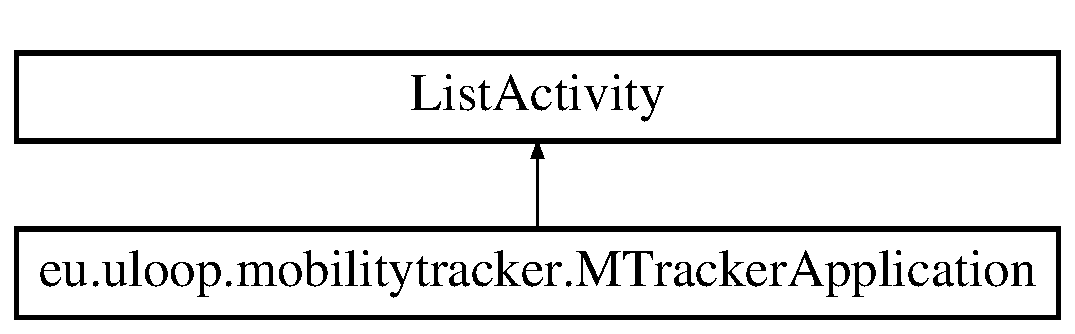
\includegraphics[height=2.000000cm]{classeu_1_1uloop_1_1mobilitytracker_1_1MTrackerApplication}
\end{center}
\end{figure}
\subsection*{Public Member Functions}
\begin{DoxyCompactItemize}
\item 
boolean \hyperlink{classeu_1_1uloop_1_1mobilitytracker_1_1MTrackerApplication_a5c70e976a690da29761f108c08b787d2}{on\+Create\+Options\+Menu} (Menu menu)
\item 
boolean \hyperlink{classeu_1_1uloop_1_1mobilitytracker_1_1MTrackerApplication_a631a41a9ee16147f50de66b940fd02e7}{on\+Options\+Item\+Selected} (Menu\+Item item)
\end{DoxyCompactItemize}
\subsection*{Protected Member Functions}
\begin{DoxyCompactItemize}
\item 
void \hyperlink{classeu_1_1uloop_1_1mobilitytracker_1_1MTrackerApplication_abf76939c15ce778a376e587eb8f84ded}{on\+Create} (Bundle saved\+Instance\+State)
\item 
void \hyperlink{classeu_1_1uloop_1_1mobilitytracker_1_1MTrackerApplication_afdfea9b1742debe6a97c543af244f8bf}{on\+Start} ()
\item 
void \hyperlink{classeu_1_1uloop_1_1mobilitytracker_1_1MTrackerApplication_ad9a1d28fe98db398cda3e4659e541198}{on\+Stop} ()
\item 
void \hyperlink{classeu_1_1uloop_1_1mobilitytracker_1_1MTrackerApplication_a0a015a098e6001e4028af096330cc511}{on\+Destroy} ()
\end{DoxyCompactItemize}
\subsection*{Private Member Functions}
\begin{DoxyCompactItemize}
\item 
void \hyperlink{classeu_1_1uloop_1_1mobilitytracker_1_1MTrackerApplication_ae60069051b3aba4ff06e6635dcd3de29}{update\+List\+View} (List$<$ \hyperlink{classeu_1_1uloop_1_1mobilitytracker_1_1MTrackerAP}{M\+Tracker\+A\+P} $>$ ap\+Entries)
\end{DoxyCompactItemize}
\subsection*{Private Attributes}
\begin{DoxyCompactItemize}
\item 
\hyperlink{classeu_1_1uloop_1_1mobilitytracker_1_1MTrackerService}{M\+Tracker\+Service} \hyperlink{classeu_1_1uloop_1_1mobilitytracker_1_1MTrackerApplication_a731fac56b39d015f69211a9f6a3759e5}{m\+Bound\+Service}
\item 
boolean \hyperlink{classeu_1_1uloop_1_1mobilitytracker_1_1MTrackerApplication_a34c00e829a9027258db6291a829fa7e0}{m\+Is\+Service\+Bound} = false
\item 
Service\+Connection \hyperlink{classeu_1_1uloop_1_1mobilitytracker_1_1MTrackerApplication_a17bc5aed91845f4985a42439d6020bbb}{m\+Connection}
\end{DoxyCompactItemize}


\subsection{Detailed Description}
The Class \hyperlink{classeu_1_1uloop_1_1mobilitytracker_1_1MTrackerApplication}{M\+Tracker\+Application} is the front-\/end of the android application. It extends List\+Activity to show the list of visited access points as a List\+View. It starts the M\+Tracker server, if not running already.

\begin{DoxyAuthor}{Author}
Jonnahtan Saltarin (U\+L\+H\+T) 

Rute Sofia (U\+L\+H\+T) 

Christian da Silva Pereira (U\+L\+H\+T) 

Luis Amaral Lopes (U\+L\+H\+T)
\end{DoxyAuthor}
\begin{DoxyVersion}{Version}
3.\+0 
\end{DoxyVersion}


\subsection{Member Function Documentation}
\hypertarget{classeu_1_1uloop_1_1mobilitytracker_1_1MTrackerApplication_abf76939c15ce778a376e587eb8f84ded}{\index{eu\+::uloop\+::mobilitytracker\+::\+M\+Tracker\+Application@{eu\+::uloop\+::mobilitytracker\+::\+M\+Tracker\+Application}!on\+Create@{on\+Create}}
\index{on\+Create@{on\+Create}!eu\+::uloop\+::mobilitytracker\+::\+M\+Tracker\+Application@{eu\+::uloop\+::mobilitytracker\+::\+M\+Tracker\+Application}}
\subsubsection[{on\+Create}]{\setlength{\rightskip}{0pt plus 5cm}void eu.\+uloop.\+mobilitytracker.\+M\+Tracker\+Application.\+on\+Create (
\begin{DoxyParamCaption}
\item[{Bundle}]{saved\+Instance\+State}
\end{DoxyParamCaption}
)\hspace{0.3cm}{\ttfamily [protected]}}}\label{classeu_1_1uloop_1_1mobilitytracker_1_1MTrackerApplication_abf76939c15ce778a376e587eb8f84ded}
\hypertarget{classeu_1_1uloop_1_1mobilitytracker_1_1MTrackerApplication_a5c70e976a690da29761f108c08b787d2}{\index{eu\+::uloop\+::mobilitytracker\+::\+M\+Tracker\+Application@{eu\+::uloop\+::mobilitytracker\+::\+M\+Tracker\+Application}!on\+Create\+Options\+Menu@{on\+Create\+Options\+Menu}}
\index{on\+Create\+Options\+Menu@{on\+Create\+Options\+Menu}!eu\+::uloop\+::mobilitytracker\+::\+M\+Tracker\+Application@{eu\+::uloop\+::mobilitytracker\+::\+M\+Tracker\+Application}}
\subsubsection[{on\+Create\+Options\+Menu}]{\setlength{\rightskip}{0pt plus 5cm}boolean eu.\+uloop.\+mobilitytracker.\+M\+Tracker\+Application.\+on\+Create\+Options\+Menu (
\begin{DoxyParamCaption}
\item[{Menu}]{menu}
\end{DoxyParamCaption}
)}}\label{classeu_1_1uloop_1_1mobilitytracker_1_1MTrackerApplication_a5c70e976a690da29761f108c08b787d2}
\hypertarget{classeu_1_1uloop_1_1mobilitytracker_1_1MTrackerApplication_a0a015a098e6001e4028af096330cc511}{\index{eu\+::uloop\+::mobilitytracker\+::\+M\+Tracker\+Application@{eu\+::uloop\+::mobilitytracker\+::\+M\+Tracker\+Application}!on\+Destroy@{on\+Destroy}}
\index{on\+Destroy@{on\+Destroy}!eu\+::uloop\+::mobilitytracker\+::\+M\+Tracker\+Application@{eu\+::uloop\+::mobilitytracker\+::\+M\+Tracker\+Application}}
\subsubsection[{on\+Destroy}]{\setlength{\rightskip}{0pt plus 5cm}void eu.\+uloop.\+mobilitytracker.\+M\+Tracker\+Application.\+on\+Destroy (
\begin{DoxyParamCaption}
{}
\end{DoxyParamCaption}
)\hspace{0.3cm}{\ttfamily [protected]}}}\label{classeu_1_1uloop_1_1mobilitytracker_1_1MTrackerApplication_a0a015a098e6001e4028af096330cc511}
\hypertarget{classeu_1_1uloop_1_1mobilitytracker_1_1MTrackerApplication_a631a41a9ee16147f50de66b940fd02e7}{\index{eu\+::uloop\+::mobilitytracker\+::\+M\+Tracker\+Application@{eu\+::uloop\+::mobilitytracker\+::\+M\+Tracker\+Application}!on\+Options\+Item\+Selected@{on\+Options\+Item\+Selected}}
\index{on\+Options\+Item\+Selected@{on\+Options\+Item\+Selected}!eu\+::uloop\+::mobilitytracker\+::\+M\+Tracker\+Application@{eu\+::uloop\+::mobilitytracker\+::\+M\+Tracker\+Application}}
\subsubsection[{on\+Options\+Item\+Selected}]{\setlength{\rightskip}{0pt plus 5cm}boolean eu.\+uloop.\+mobilitytracker.\+M\+Tracker\+Application.\+on\+Options\+Item\+Selected (
\begin{DoxyParamCaption}
\item[{Menu\+Item}]{item}
\end{DoxyParamCaption}
)}}\label{classeu_1_1uloop_1_1mobilitytracker_1_1MTrackerApplication_a631a41a9ee16147f50de66b940fd02e7}
\hypertarget{classeu_1_1uloop_1_1mobilitytracker_1_1MTrackerApplication_afdfea9b1742debe6a97c543af244f8bf}{\index{eu\+::uloop\+::mobilitytracker\+::\+M\+Tracker\+Application@{eu\+::uloop\+::mobilitytracker\+::\+M\+Tracker\+Application}!on\+Start@{on\+Start}}
\index{on\+Start@{on\+Start}!eu\+::uloop\+::mobilitytracker\+::\+M\+Tracker\+Application@{eu\+::uloop\+::mobilitytracker\+::\+M\+Tracker\+Application}}
\subsubsection[{on\+Start}]{\setlength{\rightskip}{0pt plus 5cm}void eu.\+uloop.\+mobilitytracker.\+M\+Tracker\+Application.\+on\+Start (
\begin{DoxyParamCaption}
{}
\end{DoxyParamCaption}
)\hspace{0.3cm}{\ttfamily [protected]}}}\label{classeu_1_1uloop_1_1mobilitytracker_1_1MTrackerApplication_afdfea9b1742debe6a97c543af244f8bf}
\hypertarget{classeu_1_1uloop_1_1mobilitytracker_1_1MTrackerApplication_ad9a1d28fe98db398cda3e4659e541198}{\index{eu\+::uloop\+::mobilitytracker\+::\+M\+Tracker\+Application@{eu\+::uloop\+::mobilitytracker\+::\+M\+Tracker\+Application}!on\+Stop@{on\+Stop}}
\index{on\+Stop@{on\+Stop}!eu\+::uloop\+::mobilitytracker\+::\+M\+Tracker\+Application@{eu\+::uloop\+::mobilitytracker\+::\+M\+Tracker\+Application}}
\subsubsection[{on\+Stop}]{\setlength{\rightskip}{0pt plus 5cm}void eu.\+uloop.\+mobilitytracker.\+M\+Tracker\+Application.\+on\+Stop (
\begin{DoxyParamCaption}
{}
\end{DoxyParamCaption}
)\hspace{0.3cm}{\ttfamily [protected]}}}\label{classeu_1_1uloop_1_1mobilitytracker_1_1MTrackerApplication_ad9a1d28fe98db398cda3e4659e541198}
\hypertarget{classeu_1_1uloop_1_1mobilitytracker_1_1MTrackerApplication_ae60069051b3aba4ff06e6635dcd3de29}{\index{eu\+::uloop\+::mobilitytracker\+::\+M\+Tracker\+Application@{eu\+::uloop\+::mobilitytracker\+::\+M\+Tracker\+Application}!update\+List\+View@{update\+List\+View}}
\index{update\+List\+View@{update\+List\+View}!eu\+::uloop\+::mobilitytracker\+::\+M\+Tracker\+Application@{eu\+::uloop\+::mobilitytracker\+::\+M\+Tracker\+Application}}
\subsubsection[{update\+List\+View}]{\setlength{\rightskip}{0pt plus 5cm}void eu.\+uloop.\+mobilitytracker.\+M\+Tracker\+Application.\+update\+List\+View (
\begin{DoxyParamCaption}
\item[{List$<$ {\bf M\+Tracker\+A\+P} $>$}]{ap\+Entries}
\end{DoxyParamCaption}
)\hspace{0.3cm}{\ttfamily [private]}}}\label{classeu_1_1uloop_1_1mobilitytracker_1_1MTrackerApplication_ae60069051b3aba4ff06e6635dcd3de29}
Update the List\+View, cleaning the actual values and populating it with the values on ap\+Entries.


\begin{DoxyParams}{Parameters}
{\em ap\+Entries} & the new access point entries to be shown. \\
\hline
\end{DoxyParams}


\subsection{Member Data Documentation}
\hypertarget{classeu_1_1uloop_1_1mobilitytracker_1_1MTrackerApplication_a731fac56b39d015f69211a9f6a3759e5}{\index{eu\+::uloop\+::mobilitytracker\+::\+M\+Tracker\+Application@{eu\+::uloop\+::mobilitytracker\+::\+M\+Tracker\+Application}!m\+Bound\+Service@{m\+Bound\+Service}}
\index{m\+Bound\+Service@{m\+Bound\+Service}!eu\+::uloop\+::mobilitytracker\+::\+M\+Tracker\+Application@{eu\+::uloop\+::mobilitytracker\+::\+M\+Tracker\+Application}}
\subsubsection[{m\+Bound\+Service}]{\setlength{\rightskip}{0pt plus 5cm}{\bf M\+Tracker\+Service} eu.\+uloop.\+mobilitytracker.\+M\+Tracker\+Application.\+m\+Bound\+Service\hspace{0.3cm}{\ttfamily [private]}}}\label{classeu_1_1uloop_1_1mobilitytracker_1_1MTrackerApplication_a731fac56b39d015f69211a9f6a3759e5}
The M\+Tracker service to be bounded. \hypertarget{classeu_1_1uloop_1_1mobilitytracker_1_1MTrackerApplication_a17bc5aed91845f4985a42439d6020bbb}{\index{eu\+::uloop\+::mobilitytracker\+::\+M\+Tracker\+Application@{eu\+::uloop\+::mobilitytracker\+::\+M\+Tracker\+Application}!m\+Connection@{m\+Connection}}
\index{m\+Connection@{m\+Connection}!eu\+::uloop\+::mobilitytracker\+::\+M\+Tracker\+Application@{eu\+::uloop\+::mobilitytracker\+::\+M\+Tracker\+Application}}
\subsubsection[{m\+Connection}]{\setlength{\rightskip}{0pt plus 5cm}Service\+Connection eu.\+uloop.\+mobilitytracker.\+M\+Tracker\+Application.\+m\+Connection\hspace{0.3cm}{\ttfamily [private]}}}\label{classeu_1_1uloop_1_1mobilitytracker_1_1MTrackerApplication_a17bc5aed91845f4985a42439d6020bbb}
{\bfseries Initial value\+:}
\begin{DoxyCode}
= \textcolor{keyword}{new} ServiceConnection() \{
            \textcolor{keyword}{public} \textcolor{keywordtype}{void} onServiceConnected(ComponentName className, IBinder service) \{
                \hyperlink{classeu_1_1uloop_1_1mobilitytracker_1_1MTrackerApplication_a731fac56b39d015f69211a9f6a3759e5}{mBoundService} = ((MTrackerService.LocalBinder)service).getService();
                        \hyperlink{classeu_1_1uloop_1_1mobilitytracker_1_1MTrackerApplication_a34c00e829a9027258db6291a829fa7e0}{mIsServiceBound} = \textcolor{keyword}{true};
                        \hyperlink{classeu_1_1uloop_1_1mobilitytracker_1_1MTrackerApplication_ae60069051b3aba4ff06e6635dcd3de29}{updateListView} (\hyperlink{classeu_1_1uloop_1_1mobilitytracker_1_1MTrackerApplication_a731fac56b39d015f69211a9f6a3759e5}{mBoundService}.
      \hyperlink{classeu_1_1uloop_1_1mobilitytracker_1_1MTrackerService_ace7c25f76f1ec7b2cfc4e5a4b28f68e9}{getData}());
                        \hyperlink{classeu_1_1uloop_1_1mobilitytracker_1_1MTrackerApplication_a731fac56b39d015f69211a9f6a3759e5}{mBoundService}.\hyperlink{classeu_1_1uloop_1_1mobilitytracker_1_1MTrackerService_a5332e648f938ae1255c4b12aa0d82054}{setOnStateChangeListener}(
                            \textcolor{keyword}{new} DataBaseChangeListener() \{
                                \textcolor{keyword}{public} \textcolor{keywordtype}{void} onDataBaseChange(List<MTrackerAP> apEntries) \{
                                        \hyperlink{classeu_1_1uloop_1_1mobilitytracker_1_1MTrackerApplication_ae60069051b3aba4ff06e6635dcd3de29}{updateListView} (apEntries);
                                \}
                                \textcolor{keyword}{public} \textcolor{keywordtype}{void} onStatusMessageChange(String newMessage)  \{
                                        ((TextView)findViewById(R.id.infoText)).setText(newMessage);
                                \}
                                \}
                        );
            \}

            \textcolor{keyword}{public} \textcolor{keywordtype}{void} onServiceDisconnected(ComponentName className) \{
                \hyperlink{classeu_1_1uloop_1_1mobilitytracker_1_1MTrackerApplication_a731fac56b39d015f69211a9f6a3759e5}{mBoundService}.\hyperlink{classeu_1_1uloop_1_1mobilitytracker_1_1MTrackerService_a5f1b2bb03919db654a59d69681a575e7}{clearOnStateChangeListeners} ();
                \hyperlink{classeu_1_1uloop_1_1mobilitytracker_1_1MTrackerApplication_a731fac56b39d015f69211a9f6a3759e5}{mBoundService} = null;
                \hyperlink{classeu_1_1uloop_1_1mobilitytracker_1_1MTrackerApplication_a34c00e829a9027258db6291a829fa7e0}{mIsServiceBound} = \textcolor{keyword}{false};
            \}
        \}
\end{DoxyCode}
The Connection to the M\+Tracker service. When the service is successfully connected, it loads the List\+View with the initial data and creates a listener on the M\+Tracker service that re-\/populates the data on the List\+View any tame the Data\+Base changes \hypertarget{classeu_1_1uloop_1_1mobilitytracker_1_1MTrackerApplication_a34c00e829a9027258db6291a829fa7e0}{\index{eu\+::uloop\+::mobilitytracker\+::\+M\+Tracker\+Application@{eu\+::uloop\+::mobilitytracker\+::\+M\+Tracker\+Application}!m\+Is\+Service\+Bound@{m\+Is\+Service\+Bound}}
\index{m\+Is\+Service\+Bound@{m\+Is\+Service\+Bound}!eu\+::uloop\+::mobilitytracker\+::\+M\+Tracker\+Application@{eu\+::uloop\+::mobilitytracker\+::\+M\+Tracker\+Application}}
\subsubsection[{m\+Is\+Service\+Bound}]{\setlength{\rightskip}{0pt plus 5cm}boolean eu.\+uloop.\+mobilitytracker.\+M\+Tracker\+Application.\+m\+Is\+Service\+Bound = false\hspace{0.3cm}{\ttfamily [private]}}}\label{classeu_1_1uloop_1_1mobilitytracker_1_1MTrackerApplication_a34c00e829a9027258db6291a829fa7e0}
Indicates if the M\+Tracker service has been bounded successfully. 

The documentation for this class was generated from the following file\+:\begin{DoxyCompactItemize}
\item 
src/eu/uloop/mobilitytracker/\hyperlink{MTrackerApplication_8java}{M\+Tracker\+Application.\+java}\end{DoxyCompactItemize}

\hypertarget{classeu_1_1uloop_1_1mobilitytracker_1_1MTrackerDataSource}{\section{eu.\+uloop.\+mobilitytracker.\+M\+Tracker\+Data\+Source Class Reference}
\label{classeu_1_1uloop_1_1mobilitytracker_1_1MTrackerDataSource}\index{eu.\+uloop.\+mobilitytracker.\+M\+Tracker\+Data\+Source@{eu.\+uloop.\+mobilitytracker.\+M\+Tracker\+Data\+Source}}
}
\subsection*{Public Member Functions}
\begin{DoxyCompactItemize}
\item 
\hyperlink{classeu_1_1uloop_1_1mobilitytracker_1_1MTrackerDataSource_af693f54273c35dc8324f963ff51f9444}{M\+Tracker\+Data\+Source} (Context context)
\item 
void \hyperlink{classeu_1_1uloop_1_1mobilitytracker_1_1MTrackerDataSource_aaf04828bd8494b7b1233bcc67fe16e7c}{open\+D\+B} (boolean writable)  throws S\+Q\+L\+Exception 
\item 
void \hyperlink{classeu_1_1uloop_1_1mobilitytracker_1_1MTrackerDataSource_af572eeea7eeca0462856542130e48a4a}{close\+D\+B} ()
\item 
long \hyperlink{classeu_1_1uloop_1_1mobilitytracker_1_1MTrackerDataSource_a5521c1c8f4b28344d7f251bf6ab96410}{get\+Num\+A\+P} ()
\item 
long \hyperlink{classeu_1_1uloop_1_1mobilitytracker_1_1MTrackerDataSource_a9e302a7eaf34e77b353863defaea19cc}{register\+New\+A\+P} (\hyperlink{classeu_1_1uloop_1_1mobilitytracker_1_1MTrackerAP}{M\+Tracker\+A\+P} ap)
\item 
boolean \hyperlink{classeu_1_1uloop_1_1mobilitytracker_1_1MTrackerDataSource_a20a7d39450e6ceed0b25e02f12568450}{update\+A\+P} (\hyperlink{classeu_1_1uloop_1_1mobilitytracker_1_1MTrackerAP}{M\+Tracker\+A\+P} ap)
\item 
\hyperlink{classeu_1_1uloop_1_1mobilitytracker_1_1MTrackerAP}{M\+Tracker\+A\+P} \hyperlink{classeu_1_1uloop_1_1mobilitytracker_1_1MTrackerDataSource_a7197573addd0912c6dae79567ab22a20}{get\+A\+P} (String bssid)
\item 
boolean \hyperlink{classeu_1_1uloop_1_1mobilitytracker_1_1MTrackerDataSource_ad6560b92283afc15dafdc2a5d702d9cf}{has\+A\+P} (String bssid)
\item 
Map$<$ String, \hyperlink{classeu_1_1uloop_1_1mobilitytracker_1_1MTrackerAP}{M\+Tracker\+A\+P} $>$ \hyperlink{classeu_1_1uloop_1_1mobilitytracker_1_1MTrackerDataSource_ac6aa292fea98d121c0ae0ccf549dc7fa}{get\+All\+A\+P} ()
\item 
Map$<$ String, \hyperlink{classeu_1_1uloop_1_1mobilitytracker_1_1MTrackerAP}{M\+Tracker\+A\+P} $>$ \hyperlink{classeu_1_1uloop_1_1mobilitytracker_1_1MTrackerDataSource_a55e5a52b26d01e60ca08757cf94e8b41}{get\+All\+A\+P} (List$<$ Scan\+Result $>$ available\+A\+P)
\item 
\hyperlink{classeu_1_1uloop_1_1mobilitytracker_1_1MTrackerAP}{M\+Tracker\+A\+P} \hyperlink{classeu_1_1uloop_1_1mobilitytracker_1_1MTrackerDataSource_a4f9666c05b19fba1bfceb9a0734390da}{get\+Best\+A\+P} ()
\item 
\hyperlink{classeu_1_1uloop_1_1mobilitytracker_1_1MTrackerAP}{M\+Tracker\+A\+P} \hyperlink{classeu_1_1uloop_1_1mobilitytracker_1_1MTrackerDataSource_a52bae6dd4aaa9f81280d4cb421360c39}{get\+Best\+A\+P} (List$<$ Scan\+Result $>$ available\+A\+P)
\item 
void \hyperlink{classeu_1_1uloop_1_1mobilitytracker_1_1MTrackerDataSource_a0cee2b0f411369a93ad42572cdda102b}{write\+A\+P\+List\+To\+File} ()
\item 
long \hyperlink{classeu_1_1uloop_1_1mobilitytracker_1_1MTrackerDataSource_ac10ee62fea68a3b1f8a34bfca4e16af1}{get\+Stationary\+Time} (\hyperlink{classeu_1_1uloop_1_1mobilitytracker_1_1MTrackerAP}{M\+Tracker\+A\+P} ap)
\item 
long \hyperlink{classeu_1_1uloop_1_1mobilitytracker_1_1MTrackerDataSource_a026e23013cc872da728dea53e7dde5fc}{get\+Stationary\+Time\+By\+Moment} (\hyperlink{classeu_1_1uloop_1_1mobilitytracker_1_1MTrackerAP}{M\+Tracker\+A\+P} ap, int day\+Of\+The\+Week)
\item 
long \hyperlink{classeu_1_1uloop_1_1mobilitytracker_1_1MTrackerDataSource_add0518908b40874c8752a3c7de05a9e5}{count\+Visits} (\hyperlink{classeu_1_1uloop_1_1mobilitytracker_1_1MTrackerAP}{M\+Tracker\+A\+P} ap)
\item 
double \hyperlink{classeu_1_1uloop_1_1mobilitytracker_1_1MTrackerDataSource_a56dc7ff72205459b80fee65474373162}{get\+Rank} (\hyperlink{classeu_1_1uloop_1_1mobilitytracker_1_1MTrackerAP}{M\+Tracker\+A\+P} ap)
\item 
double \hyperlink{classeu_1_1uloop_1_1mobilitytracker_1_1MTrackerDataSource_a3a61d8225caa68d8dd9e3047606e6611}{get\+Instantaneous\+Rank} (\hyperlink{classeu_1_1uloop_1_1mobilitytracker_1_1MTrackerAP}{M\+Tracker\+A\+P} ap, Long current\+Duration)
\item 
long \hyperlink{classeu_1_1uloop_1_1mobilitytracker_1_1MTrackerDataSource_a01c48031ea84bb65aee99a43c55ab38f}{register\+New\+Visit} (String S\+S\+I\+D, String B\+S\+S\+I\+D, Long start\+Time, Long end\+Time)
\item 
boolean \hyperlink{classeu_1_1uloop_1_1mobilitytracker_1_1MTrackerDataSource_ac1648a220f4adaf41bc3fb8980d15153}{update\+Visit} (long \+\_\+id, String S\+S\+I\+D, String B\+S\+S\+I\+D, Long start\+Time, Long end\+Time)
\item 
List$<$ \hyperlink{classeu_1_1uloop_1_1mobilitytracker_1_1MTrackerVisit}{M\+Tracker\+Visit} $>$ \hyperlink{classeu_1_1uloop_1_1mobilitytracker_1_1MTrackerDataSource_aa4dbcac64cdddb8a8d4a78b613d06dac}{get\+All\+Visits} ()
\item 
List$<$ String $>$ \hyperlink{classeu_1_1uloop_1_1mobilitytracker_1_1MTrackerDataSource_a307681e571f1edfca036f8f0eacc3016}{get\+All\+Visits\+String} (\hyperlink{classeu_1_1uloop_1_1mobilitytracker_1_1MTrackerAP}{M\+Tracker\+A\+P} ap)
\item 
long \hyperlink{classeu_1_1uloop_1_1mobilitytracker_1_1MTrackerDataSource_a3e83317ed2eb0632398c235b7209b92c}{get\+Num\+Visits} ()
\item 
void \hyperlink{classeu_1_1uloop_1_1mobilitytracker_1_1MTrackerDataSource_a65f0f4c7635c82b15cea46b5de9ab3a4}{write\+Visit\+List\+To\+File} ()
\end{DoxyCompactItemize}
\subsection*{Private Member Functions}
\begin{DoxyCompactItemize}
\item 
\hyperlink{classeu_1_1uloop_1_1mobilitytracker_1_1MTrackerAP}{M\+Tracker\+A\+P} \hyperlink{classeu_1_1uloop_1_1mobilitytracker_1_1MTrackerDataSource_a2e2416c3e0a62bbdb71e4cff6a690668}{cursor\+To\+A\+P} (Cursor cursor)
\item 
\hyperlink{classeu_1_1uloop_1_1mobilitytracker_1_1MTrackerVisit}{M\+Tracker\+Visit} \hyperlink{classeu_1_1uloop_1_1mobilitytracker_1_1MTrackerDataSource_a694f1a1c7324237c6a78c9fa9afe56f3}{cursor\+To\+Visit} (Cursor cursor)
\end{DoxyCompactItemize}
\subsection*{Private Attributes}
\begin{DoxyCompactItemize}
\item 
S\+Q\+Lite\+Database \hyperlink{classeu_1_1uloop_1_1mobilitytracker_1_1MTrackerDataSource_a7b4d7f0a2841d00604316b03597574ab}{db}
\item 
\hyperlink{classeu_1_1uloop_1_1mobilitytracker_1_1MTrackerSQLiteHelper}{M\+Tracker\+S\+Q\+Lite\+Helper} \hyperlink{classeu_1_1uloop_1_1mobilitytracker_1_1MTrackerDataSource_a5d3a9388200101ef3d058dc1aef984f2}{db\+Helper}
\item 
boolean \hyperlink{classeu_1_1uloop_1_1mobilitytracker_1_1MTrackerDataSource_a29df0e4f00d3a69afdcc3ffb145b9ed4}{is\+Db\+Open}
\item 
Gregorian\+Calendar \hyperlink{classeu_1_1uloop_1_1mobilitytracker_1_1MTrackerDataSource_a2b7984f3b6ac7c9c7aa72430b03d8fb7}{cal}
\item 
String\mbox{[}$\,$\mbox{]} \hyperlink{classeu_1_1uloop_1_1mobilitytracker_1_1MTrackerDataSource_acd01b650db85f0c22de6fa1ab015b1c6}{all\+Columns\+Access\+Point}
\item 
String\mbox{[}$\,$\mbox{]} \hyperlink{classeu_1_1uloop_1_1mobilitytracker_1_1MTrackerDataSource_abc2816de6350ca5e04f5c882402aa4fb}{all\+Columns\+Visit}
\end{DoxyCompactItemize}


\subsection{Detailed Description}
This class provides methods to insert, update and query the application database. It also provide methods to compute certain values, like the Rank and the Stationary Time, among others.

\begin{DoxyAuthor}{Author}
Jonnahtan Saltarin (U\+L\+H\+T) 

Rute Sofia (U\+L\+H\+T) 

Christian da Silva Pereira (U\+L\+H\+T) 

Luis Amaral Lopes (U\+L\+H\+T)
\end{DoxyAuthor}
\begin{DoxyVersion}{Version}
3.\+0 
\end{DoxyVersion}


\subsection{Constructor \& Destructor Documentation}
\hypertarget{classeu_1_1uloop_1_1mobilitytracker_1_1MTrackerDataSource_af693f54273c35dc8324f963ff51f9444}{\index{eu\+::uloop\+::mobilitytracker\+::\+M\+Tracker\+Data\+Source@{eu\+::uloop\+::mobilitytracker\+::\+M\+Tracker\+Data\+Source}!M\+Tracker\+Data\+Source@{M\+Tracker\+Data\+Source}}
\index{M\+Tracker\+Data\+Source@{M\+Tracker\+Data\+Source}!eu\+::uloop\+::mobilitytracker\+::\+M\+Tracker\+Data\+Source@{eu\+::uloop\+::mobilitytracker\+::\+M\+Tracker\+Data\+Source}}
\subsubsection[{M\+Tracker\+Data\+Source}]{\setlength{\rightskip}{0pt plus 5cm}eu.\+uloop.\+mobilitytracker.\+M\+Tracker\+Data\+Source.\+M\+Tracker\+Data\+Source (
\begin{DoxyParamCaption}
\item[{Context}]{context}
\end{DoxyParamCaption}
)}}\label{classeu_1_1uloop_1_1mobilitytracker_1_1MTrackerDataSource_af693f54273c35dc8324f963ff51f9444}
Constructor that takes Android Context as input.


\begin{DoxyParams}{Parameters}
{\em context} & \\
\hline
\end{DoxyParams}


\subsection{Member Function Documentation}
\hypertarget{classeu_1_1uloop_1_1mobilitytracker_1_1MTrackerDataSource_af572eeea7eeca0462856542130e48a4a}{\index{eu\+::uloop\+::mobilitytracker\+::\+M\+Tracker\+Data\+Source@{eu\+::uloop\+::mobilitytracker\+::\+M\+Tracker\+Data\+Source}!close\+D\+B@{close\+D\+B}}
\index{close\+D\+B@{close\+D\+B}!eu\+::uloop\+::mobilitytracker\+::\+M\+Tracker\+Data\+Source@{eu\+::uloop\+::mobilitytracker\+::\+M\+Tracker\+Data\+Source}}
\subsubsection[{close\+D\+B}]{\setlength{\rightskip}{0pt plus 5cm}void eu.\+uloop.\+mobilitytracker.\+M\+Tracker\+Data\+Source.\+close\+D\+B (
\begin{DoxyParamCaption}
{}
\end{DoxyParamCaption}
)}}\label{classeu_1_1uloop_1_1mobilitytracker_1_1MTrackerDataSource_af572eeea7eeca0462856542130e48a4a}
Close the predefined M\+Tracker database. \hypertarget{classeu_1_1uloop_1_1mobilitytracker_1_1MTrackerDataSource_add0518908b40874c8752a3c7de05a9e5}{\index{eu\+::uloop\+::mobilitytracker\+::\+M\+Tracker\+Data\+Source@{eu\+::uloop\+::mobilitytracker\+::\+M\+Tracker\+Data\+Source}!count\+Visits@{count\+Visits}}
\index{count\+Visits@{count\+Visits}!eu\+::uloop\+::mobilitytracker\+::\+M\+Tracker\+Data\+Source@{eu\+::uloop\+::mobilitytracker\+::\+M\+Tracker\+Data\+Source}}
\subsubsection[{count\+Visits}]{\setlength{\rightskip}{0pt plus 5cm}long eu.\+uloop.\+mobilitytracker.\+M\+Tracker\+Data\+Source.\+count\+Visits (
\begin{DoxyParamCaption}
\item[{{\bf M\+Tracker\+A\+P}}]{ap}
\end{DoxyParamCaption}
)}}\label{classeu_1_1uloop_1_1mobilitytracker_1_1MTrackerDataSource_add0518908b40874c8752a3c7de05a9e5}
Computes the Number of visits that the node has done to a given A\+P.


\begin{DoxyParams}{Parameters}
{\em ap} & The \hyperlink{classeu_1_1uloop_1_1mobilitytracker_1_1MTrackerAP}{M\+Tracker\+A\+P} whose Stationary Time is to be computed. \\
\hline
\end{DoxyParams}
\begin{DoxyReturn}{Returns}
The number of visits. 
\end{DoxyReturn}
\hypertarget{classeu_1_1uloop_1_1mobilitytracker_1_1MTrackerDataSource_a2e2416c3e0a62bbdb71e4cff6a690668}{\index{eu\+::uloop\+::mobilitytracker\+::\+M\+Tracker\+Data\+Source@{eu\+::uloop\+::mobilitytracker\+::\+M\+Tracker\+Data\+Source}!cursor\+To\+A\+P@{cursor\+To\+A\+P}}
\index{cursor\+To\+A\+P@{cursor\+To\+A\+P}!eu\+::uloop\+::mobilitytracker\+::\+M\+Tracker\+Data\+Source@{eu\+::uloop\+::mobilitytracker\+::\+M\+Tracker\+Data\+Source}}
\subsubsection[{cursor\+To\+A\+P}]{\setlength{\rightskip}{0pt plus 5cm}{\bf M\+Tracker\+A\+P} eu.\+uloop.\+mobilitytracker.\+M\+Tracker\+Data\+Source.\+cursor\+To\+A\+P (
\begin{DoxyParamCaption}
\item[{Cursor}]{cursor}
\end{DoxyParamCaption}
)\hspace{0.3cm}{\ttfamily [private]}}}\label{classeu_1_1uloop_1_1mobilitytracker_1_1MTrackerDataSource_a2e2416c3e0a62bbdb71e4cff6a690668}
Converts a cursor pointing to a record in the A\+C\+C\+E\+S\+S\+\_\+\+P\+O\+I\+N\+T\+S table to a \hyperlink{classeu_1_1uloop_1_1mobilitytracker_1_1MTrackerAP}{M\+Tracker\+A\+P} object.


\begin{DoxyParams}{Parameters}
{\em cursor} & Cursor pointing to a record of the A\+C\+E\+S\+S\+\_\+\+P\+O\+I\+N\+T\+S table. \\
\hline
\end{DoxyParams}
\begin{DoxyReturn}{Returns}
the \hyperlink{classeu_1_1uloop_1_1mobilitytracker_1_1MTrackerAP}{M\+Tracker\+A\+P} object 
\end{DoxyReturn}
\hypertarget{classeu_1_1uloop_1_1mobilitytracker_1_1MTrackerDataSource_a694f1a1c7324237c6a78c9fa9afe56f3}{\index{eu\+::uloop\+::mobilitytracker\+::\+M\+Tracker\+Data\+Source@{eu\+::uloop\+::mobilitytracker\+::\+M\+Tracker\+Data\+Source}!cursor\+To\+Visit@{cursor\+To\+Visit}}
\index{cursor\+To\+Visit@{cursor\+To\+Visit}!eu\+::uloop\+::mobilitytracker\+::\+M\+Tracker\+Data\+Source@{eu\+::uloop\+::mobilitytracker\+::\+M\+Tracker\+Data\+Source}}
\subsubsection[{cursor\+To\+Visit}]{\setlength{\rightskip}{0pt plus 5cm}{\bf M\+Tracker\+Visit} eu.\+uloop.\+mobilitytracker.\+M\+Tracker\+Data\+Source.\+cursor\+To\+Visit (
\begin{DoxyParamCaption}
\item[{Cursor}]{cursor}
\end{DoxyParamCaption}
)\hspace{0.3cm}{\ttfamily [private]}}}\label{classeu_1_1uloop_1_1mobilitytracker_1_1MTrackerDataSource_a694f1a1c7324237c6a78c9fa9afe56f3}
\hypertarget{classeu_1_1uloop_1_1mobilitytracker_1_1MTrackerDataSource_ac6aa292fea98d121c0ae0ccf549dc7fa}{\index{eu\+::uloop\+::mobilitytracker\+::\+M\+Tracker\+Data\+Source@{eu\+::uloop\+::mobilitytracker\+::\+M\+Tracker\+Data\+Source}!get\+All\+A\+P@{get\+All\+A\+P}}
\index{get\+All\+A\+P@{get\+All\+A\+P}!eu\+::uloop\+::mobilitytracker\+::\+M\+Tracker\+Data\+Source@{eu\+::uloop\+::mobilitytracker\+::\+M\+Tracker\+Data\+Source}}
\subsubsection[{get\+All\+A\+P}]{\setlength{\rightskip}{0pt plus 5cm}Map$<$String, {\bf M\+Tracker\+A\+P}$>$ eu.\+uloop.\+mobilitytracker.\+M\+Tracker\+Data\+Source.\+get\+All\+A\+P (
\begin{DoxyParamCaption}
{}
\end{DoxyParamCaption}
)}}\label{classeu_1_1uloop_1_1mobilitytracker_1_1MTrackerDataSource_ac6aa292fea98d121c0ae0ccf549dc7fa}
Gets the all the A\+P recorded by the application on the A\+C\+C\+E\+S\+S\+\_\+\+P\+O\+I\+N\+T\+S table.

\begin{DoxyReturn}{Returns}
A map with the A\+P objects, and the bssid as key. 
\end{DoxyReturn}
\hypertarget{classeu_1_1uloop_1_1mobilitytracker_1_1MTrackerDataSource_a55e5a52b26d01e60ca08757cf94e8b41}{\index{eu\+::uloop\+::mobilitytracker\+::\+M\+Tracker\+Data\+Source@{eu\+::uloop\+::mobilitytracker\+::\+M\+Tracker\+Data\+Source}!get\+All\+A\+P@{get\+All\+A\+P}}
\index{get\+All\+A\+P@{get\+All\+A\+P}!eu\+::uloop\+::mobilitytracker\+::\+M\+Tracker\+Data\+Source@{eu\+::uloop\+::mobilitytracker\+::\+M\+Tracker\+Data\+Source}}
\subsubsection[{get\+All\+A\+P}]{\setlength{\rightskip}{0pt plus 5cm}Map$<$String, {\bf M\+Tracker\+A\+P}$>$ eu.\+uloop.\+mobilitytracker.\+M\+Tracker\+Data\+Source.\+get\+All\+A\+P (
\begin{DoxyParamCaption}
\item[{List$<$ Scan\+Result $>$}]{available\+A\+P}
\end{DoxyParamCaption}
)}}\label{classeu_1_1uloop_1_1mobilitytracker_1_1MTrackerDataSource_a55e5a52b26d01e60ca08757cf94e8b41}
Gets the all the A\+P recorded by the application on the A\+C\+C\+E\+S\+S\+\_\+\+P\+O\+I\+N\+T\+S table, and the return only the ones that are also available in the List of Scan\+Result.

\begin{DoxyReturn}{Returns}
A map with the A\+P objects, and the bssid as key. 
\end{DoxyReturn}
\hypertarget{classeu_1_1uloop_1_1mobilitytracker_1_1MTrackerDataSource_aa4dbcac64cdddb8a8d4a78b613d06dac}{\index{eu\+::uloop\+::mobilitytracker\+::\+M\+Tracker\+Data\+Source@{eu\+::uloop\+::mobilitytracker\+::\+M\+Tracker\+Data\+Source}!get\+All\+Visits@{get\+All\+Visits}}
\index{get\+All\+Visits@{get\+All\+Visits}!eu\+::uloop\+::mobilitytracker\+::\+M\+Tracker\+Data\+Source@{eu\+::uloop\+::mobilitytracker\+::\+M\+Tracker\+Data\+Source}}
\subsubsection[{get\+All\+Visits}]{\setlength{\rightskip}{0pt plus 5cm}List$<${\bf M\+Tracker\+Visit}$>$ eu.\+uloop.\+mobilitytracker.\+M\+Tracker\+Data\+Source.\+get\+All\+Visits (
\begin{DoxyParamCaption}
{}
\end{DoxyParamCaption}
)}}\label{classeu_1_1uloop_1_1mobilitytracker_1_1MTrackerDataSource_aa4dbcac64cdddb8a8d4a78b613d06dac}
Get a List with all the visit objects stored in the database. \hypertarget{classeu_1_1uloop_1_1mobilitytracker_1_1MTrackerDataSource_a307681e571f1edfca036f8f0eacc3016}{\index{eu\+::uloop\+::mobilitytracker\+::\+M\+Tracker\+Data\+Source@{eu\+::uloop\+::mobilitytracker\+::\+M\+Tracker\+Data\+Source}!get\+All\+Visits\+String@{get\+All\+Visits\+String}}
\index{get\+All\+Visits\+String@{get\+All\+Visits\+String}!eu\+::uloop\+::mobilitytracker\+::\+M\+Tracker\+Data\+Source@{eu\+::uloop\+::mobilitytracker\+::\+M\+Tracker\+Data\+Source}}
\subsubsection[{get\+All\+Visits\+String}]{\setlength{\rightskip}{0pt plus 5cm}List$<$String$>$ eu.\+uloop.\+mobilitytracker.\+M\+Tracker\+Data\+Source.\+get\+All\+Visits\+String (
\begin{DoxyParamCaption}
\item[{{\bf M\+Tracker\+A\+P}}]{ap}
\end{DoxyParamCaption}
)}}\label{classeu_1_1uloop_1_1mobilitytracker_1_1MTrackerDataSource_a307681e571f1edfca036f8f0eacc3016}
\hypertarget{classeu_1_1uloop_1_1mobilitytracker_1_1MTrackerDataSource_a7197573addd0912c6dae79567ab22a20}{\index{eu\+::uloop\+::mobilitytracker\+::\+M\+Tracker\+Data\+Source@{eu\+::uloop\+::mobilitytracker\+::\+M\+Tracker\+Data\+Source}!get\+A\+P@{get\+A\+P}}
\index{get\+A\+P@{get\+A\+P}!eu\+::uloop\+::mobilitytracker\+::\+M\+Tracker\+Data\+Source@{eu\+::uloop\+::mobilitytracker\+::\+M\+Tracker\+Data\+Source}}
\subsubsection[{get\+A\+P}]{\setlength{\rightskip}{0pt plus 5cm}{\bf M\+Tracker\+A\+P} eu.\+uloop.\+mobilitytracker.\+M\+Tracker\+Data\+Source.\+get\+A\+P (
\begin{DoxyParamCaption}
\item[{String}]{bssid}
\end{DoxyParamCaption}
)}}\label{classeu_1_1uloop_1_1mobilitytracker_1_1MTrackerDataSource_a7197573addd0912c6dae79567ab22a20}
Gets an A\+P already registered by the application.


\begin{DoxyParams}{Parameters}
{\em bssid} & The ssid of the A\+P which information should be returned \\
\hline
\end{DoxyParams}
\begin{DoxyReturn}{Returns}
the \hyperlink{classeu_1_1uloop_1_1mobilitytracker_1_1MTrackerAP}{M\+Tracker\+A\+P} object, null if not found. 
\end{DoxyReturn}
\hypertarget{classeu_1_1uloop_1_1mobilitytracker_1_1MTrackerDataSource_a4f9666c05b19fba1bfceb9a0734390da}{\index{eu\+::uloop\+::mobilitytracker\+::\+M\+Tracker\+Data\+Source@{eu\+::uloop\+::mobilitytracker\+::\+M\+Tracker\+Data\+Source}!get\+Best\+A\+P@{get\+Best\+A\+P}}
\index{get\+Best\+A\+P@{get\+Best\+A\+P}!eu\+::uloop\+::mobilitytracker\+::\+M\+Tracker\+Data\+Source@{eu\+::uloop\+::mobilitytracker\+::\+M\+Tracker\+Data\+Source}}
\subsubsection[{get\+Best\+A\+P}]{\setlength{\rightskip}{0pt plus 5cm}{\bf M\+Tracker\+A\+P} eu.\+uloop.\+mobilitytracker.\+M\+Tracker\+Data\+Source.\+get\+Best\+A\+P (
\begin{DoxyParamCaption}
{}
\end{DoxyParamCaption}
)}}\label{classeu_1_1uloop_1_1mobilitytracker_1_1MTrackerDataSource_a4f9666c05b19fba1bfceb9a0734390da}
Checks all the A\+P registered by the application and return the one with the highest Rank.

\begin{DoxyReturn}{Returns}
the best A\+P registered by the application. 
\end{DoxyReturn}
\hypertarget{classeu_1_1uloop_1_1mobilitytracker_1_1MTrackerDataSource_a52bae6dd4aaa9f81280d4cb421360c39}{\index{eu\+::uloop\+::mobilitytracker\+::\+M\+Tracker\+Data\+Source@{eu\+::uloop\+::mobilitytracker\+::\+M\+Tracker\+Data\+Source}!get\+Best\+A\+P@{get\+Best\+A\+P}}
\index{get\+Best\+A\+P@{get\+Best\+A\+P}!eu\+::uloop\+::mobilitytracker\+::\+M\+Tracker\+Data\+Source@{eu\+::uloop\+::mobilitytracker\+::\+M\+Tracker\+Data\+Source}}
\subsubsection[{get\+Best\+A\+P}]{\setlength{\rightskip}{0pt plus 5cm}{\bf M\+Tracker\+A\+P} eu.\+uloop.\+mobilitytracker.\+M\+Tracker\+Data\+Source.\+get\+Best\+A\+P (
\begin{DoxyParamCaption}
\item[{List$<$ Scan\+Result $>$}]{available\+A\+P}
\end{DoxyParamCaption}
)}}\label{classeu_1_1uloop_1_1mobilitytracker_1_1MTrackerDataSource_a52bae6dd4aaa9f81280d4cb421360c39}
Checks the A\+Ps registered by the application and available in the List of Scan\+Result, and the return the one with the highest rank.

\begin{DoxyReturn}{Returns}
the best A\+P registered by the application. 
\end{DoxyReturn}
\hypertarget{classeu_1_1uloop_1_1mobilitytracker_1_1MTrackerDataSource_a3a61d8225caa68d8dd9e3047606e6611}{\index{eu\+::uloop\+::mobilitytracker\+::\+M\+Tracker\+Data\+Source@{eu\+::uloop\+::mobilitytracker\+::\+M\+Tracker\+Data\+Source}!get\+Instantaneous\+Rank@{get\+Instantaneous\+Rank}}
\index{get\+Instantaneous\+Rank@{get\+Instantaneous\+Rank}!eu\+::uloop\+::mobilitytracker\+::\+M\+Tracker\+Data\+Source@{eu\+::uloop\+::mobilitytracker\+::\+M\+Tracker\+Data\+Source}}
\subsubsection[{get\+Instantaneous\+Rank}]{\setlength{\rightskip}{0pt plus 5cm}double eu.\+uloop.\+mobilitytracker.\+M\+Tracker\+Data\+Source.\+get\+Instantaneous\+Rank (
\begin{DoxyParamCaption}
\item[{{\bf M\+Tracker\+A\+P}}]{ap, }
\item[{Long}]{current\+Duration}
\end{DoxyParamCaption}
)}}\label{classeu_1_1uloop_1_1mobilitytracker_1_1MTrackerDataSource_a3a61d8225caa68d8dd9e3047606e6611}
Test Method to compute the Rank of this node towards a given A\+P, taking into consideration the current visit time.


\begin{DoxyParams}{Parameters}
{\em ap} & The \hyperlink{classeu_1_1uloop_1_1mobilitytracker_1_1MTrackerAP}{M\+Tracker\+A\+P} whose Stationary Time is to be computed. \\
\hline
{\em current\+Duration} & current connection time. \\
\hline
\end{DoxyParams}
\begin{DoxyReturn}{Returns}
The number of visits. 
\end{DoxyReturn}
\hypertarget{classeu_1_1uloop_1_1mobilitytracker_1_1MTrackerDataSource_a5521c1c8f4b28344d7f251bf6ab96410}{\index{eu\+::uloop\+::mobilitytracker\+::\+M\+Tracker\+Data\+Source@{eu\+::uloop\+::mobilitytracker\+::\+M\+Tracker\+Data\+Source}!get\+Num\+A\+P@{get\+Num\+A\+P}}
\index{get\+Num\+A\+P@{get\+Num\+A\+P}!eu\+::uloop\+::mobilitytracker\+::\+M\+Tracker\+Data\+Source@{eu\+::uloop\+::mobilitytracker\+::\+M\+Tracker\+Data\+Source}}
\subsubsection[{get\+Num\+A\+P}]{\setlength{\rightskip}{0pt plus 5cm}long eu.\+uloop.\+mobilitytracker.\+M\+Tracker\+Data\+Source.\+get\+Num\+A\+P (
\begin{DoxyParamCaption}
{}
\end{DoxyParamCaption}
)}}\label{classeu_1_1uloop_1_1mobilitytracker_1_1MTrackerDataSource_a5521c1c8f4b28344d7f251bf6ab96410}
Gets the number of records in the A\+C\+C\+E\+S\+S\+\_\+\+P\+O\+I\+N\+T\+S table. This is, the number of A\+P registered on the application.

\begin{DoxyReturn}{Returns}
the number of A\+P registered by the application. 
\end{DoxyReturn}
\hypertarget{classeu_1_1uloop_1_1mobilitytracker_1_1MTrackerDataSource_a3e83317ed2eb0632398c235b7209b92c}{\index{eu\+::uloop\+::mobilitytracker\+::\+M\+Tracker\+Data\+Source@{eu\+::uloop\+::mobilitytracker\+::\+M\+Tracker\+Data\+Source}!get\+Num\+Visits@{get\+Num\+Visits}}
\index{get\+Num\+Visits@{get\+Num\+Visits}!eu\+::uloop\+::mobilitytracker\+::\+M\+Tracker\+Data\+Source@{eu\+::uloop\+::mobilitytracker\+::\+M\+Tracker\+Data\+Source}}
\subsubsection[{get\+Num\+Visits}]{\setlength{\rightskip}{0pt plus 5cm}long eu.\+uloop.\+mobilitytracker.\+M\+Tracker\+Data\+Source.\+get\+Num\+Visits (
\begin{DoxyParamCaption}
{}
\end{DoxyParamCaption}
)}}\label{classeu_1_1uloop_1_1mobilitytracker_1_1MTrackerDataSource_a3e83317ed2eb0632398c235b7209b92c}
Get the number of visits registered in the database. \hypertarget{classeu_1_1uloop_1_1mobilitytracker_1_1MTrackerDataSource_a56dc7ff72205459b80fee65474373162}{\index{eu\+::uloop\+::mobilitytracker\+::\+M\+Tracker\+Data\+Source@{eu\+::uloop\+::mobilitytracker\+::\+M\+Tracker\+Data\+Source}!get\+Rank@{get\+Rank}}
\index{get\+Rank@{get\+Rank}!eu\+::uloop\+::mobilitytracker\+::\+M\+Tracker\+Data\+Source@{eu\+::uloop\+::mobilitytracker\+::\+M\+Tracker\+Data\+Source}}
\subsubsection[{get\+Rank}]{\setlength{\rightskip}{0pt plus 5cm}double eu.\+uloop.\+mobilitytracker.\+M\+Tracker\+Data\+Source.\+get\+Rank (
\begin{DoxyParamCaption}
\item[{{\bf M\+Tracker\+A\+P}}]{ap}
\end{DoxyParamCaption}
)}}\label{classeu_1_1uloop_1_1mobilitytracker_1_1MTrackerDataSource_a56dc7ff72205459b80fee65474373162}
Computes the Rank of this node towards a given A\+P. The Rank is computed as


\begin{DoxyParams}{Parameters}
{\em ap} & The \hyperlink{classeu_1_1uloop_1_1mobilitytracker_1_1MTrackerAP}{M\+Tracker\+A\+P} whose Stationary Time is to be computed. \\
\hline
\end{DoxyParams}
\begin{DoxyReturn}{Returns}
The number of visits. 
\end{DoxyReturn}
\hypertarget{classeu_1_1uloop_1_1mobilitytracker_1_1MTrackerDataSource_ac10ee62fea68a3b1f8a34bfca4e16af1}{\index{eu\+::uloop\+::mobilitytracker\+::\+M\+Tracker\+Data\+Source@{eu\+::uloop\+::mobilitytracker\+::\+M\+Tracker\+Data\+Source}!get\+Stationary\+Time@{get\+Stationary\+Time}}
\index{get\+Stationary\+Time@{get\+Stationary\+Time}!eu\+::uloop\+::mobilitytracker\+::\+M\+Tracker\+Data\+Source@{eu\+::uloop\+::mobilitytracker\+::\+M\+Tracker\+Data\+Source}}
\subsubsection[{get\+Stationary\+Time}]{\setlength{\rightskip}{0pt plus 5cm}long eu.\+uloop.\+mobilitytracker.\+M\+Tracker\+Data\+Source.\+get\+Stationary\+Time (
\begin{DoxyParamCaption}
\item[{{\bf M\+Tracker\+A\+P}}]{ap}
\end{DoxyParamCaption}
)}}\label{classeu_1_1uloop_1_1mobilitytracker_1_1MTrackerDataSource_ac10ee62fea68a3b1f8a34bfca4e16af1}
Computes the Stationary Time for a given A\+P.


\begin{DoxyParams}{Parameters}
{\em ap} & The \hyperlink{classeu_1_1uloop_1_1mobilitytracker_1_1MTrackerAP}{M\+Tracker\+A\+P} whose Stationary Time is to be computed. \\
\hline
\end{DoxyParams}
\begin{DoxyReturn}{Returns}
The stationary time for the given A\+P. 
\end{DoxyReturn}
\hypertarget{classeu_1_1uloop_1_1mobilitytracker_1_1MTrackerDataSource_a026e23013cc872da728dea53e7dde5fc}{\index{eu\+::uloop\+::mobilitytracker\+::\+M\+Tracker\+Data\+Source@{eu\+::uloop\+::mobilitytracker\+::\+M\+Tracker\+Data\+Source}!get\+Stationary\+Time\+By\+Moment@{get\+Stationary\+Time\+By\+Moment}}
\index{get\+Stationary\+Time\+By\+Moment@{get\+Stationary\+Time\+By\+Moment}!eu\+::uloop\+::mobilitytracker\+::\+M\+Tracker\+Data\+Source@{eu\+::uloop\+::mobilitytracker\+::\+M\+Tracker\+Data\+Source}}
\subsubsection[{get\+Stationary\+Time\+By\+Moment}]{\setlength{\rightskip}{0pt plus 5cm}long eu.\+uloop.\+mobilitytracker.\+M\+Tracker\+Data\+Source.\+get\+Stationary\+Time\+By\+Moment (
\begin{DoxyParamCaption}
\item[{{\bf M\+Tracker\+A\+P}}]{ap, }
\item[{int}]{day\+Of\+The\+Week}
\end{DoxyParamCaption}
)}}\label{classeu_1_1uloop_1_1mobilitytracker_1_1MTrackerDataSource_a026e23013cc872da728dea53e7dde5fc}
Computes the Stationary Time for a given A\+P, only taking into consideration records for a given Day of the Week.


\begin{DoxyParams}{Parameters}
{\em ap} & The \hyperlink{classeu_1_1uloop_1_1mobilitytracker_1_1MTrackerAP}{M\+Tracker\+A\+P} whose Stationary Time is to be computed. \\
\hline
{\em day\+Of\+The\+Week} & Day of the week that will restrict the computation of the stationary time. \\
\hline
\end{DoxyParams}
\begin{DoxyReturn}{Returns}
The stationary time for the given A\+P. 
\end{DoxyReturn}
\hypertarget{classeu_1_1uloop_1_1mobilitytracker_1_1MTrackerDataSource_ad6560b92283afc15dafdc2a5d702d9cf}{\index{eu\+::uloop\+::mobilitytracker\+::\+M\+Tracker\+Data\+Source@{eu\+::uloop\+::mobilitytracker\+::\+M\+Tracker\+Data\+Source}!has\+A\+P@{has\+A\+P}}
\index{has\+A\+P@{has\+A\+P}!eu\+::uloop\+::mobilitytracker\+::\+M\+Tracker\+Data\+Source@{eu\+::uloop\+::mobilitytracker\+::\+M\+Tracker\+Data\+Source}}
\subsubsection[{has\+A\+P}]{\setlength{\rightskip}{0pt plus 5cm}boolean eu.\+uloop.\+mobilitytracker.\+M\+Tracker\+Data\+Source.\+has\+A\+P (
\begin{DoxyParamCaption}
\item[{String}]{bssid}
\end{DoxyParamCaption}
)}}\label{classeu_1_1uloop_1_1mobilitytracker_1_1MTrackerDataSource_ad6560b92283afc15dafdc2a5d702d9cf}
Checks if a given A\+P has already been registered by the application.


\begin{DoxyParams}{Parameters}
{\em bssid} & The ssid of the A\+P \\
\hline
\end{DoxyParams}
\begin{DoxyReturn}{Returns}
true, if A\+P has already been registered by the application, false otherwise. 
\end{DoxyReturn}
\hypertarget{classeu_1_1uloop_1_1mobilitytracker_1_1MTrackerDataSource_aaf04828bd8494b7b1233bcc67fe16e7c}{\index{eu\+::uloop\+::mobilitytracker\+::\+M\+Tracker\+Data\+Source@{eu\+::uloop\+::mobilitytracker\+::\+M\+Tracker\+Data\+Source}!open\+D\+B@{open\+D\+B}}
\index{open\+D\+B@{open\+D\+B}!eu\+::uloop\+::mobilitytracker\+::\+M\+Tracker\+Data\+Source@{eu\+::uloop\+::mobilitytracker\+::\+M\+Tracker\+Data\+Source}}
\subsubsection[{open\+D\+B}]{\setlength{\rightskip}{0pt plus 5cm}void eu.\+uloop.\+mobilitytracker.\+M\+Tracker\+Data\+Source.\+open\+D\+B (
\begin{DoxyParamCaption}
\item[{boolean}]{writable}
\end{DoxyParamCaption}
) throws S\+Q\+L\+Exception}}\label{classeu_1_1uloop_1_1mobilitytracker_1_1MTrackerDataSource_aaf04828bd8494b7b1233bcc67fe16e7c}
Opens the predefined M\+Tracker database.


\begin{DoxyParams}{Parameters}
{\em writable} & \\
\hline
\end{DoxyParams}

\begin{DoxyExceptions}{Exceptions}
{\em S\+Q\+L\+Exception} & \\
\hline
\end{DoxyExceptions}
\hypertarget{classeu_1_1uloop_1_1mobilitytracker_1_1MTrackerDataSource_a9e302a7eaf34e77b353863defaea19cc}{\index{eu\+::uloop\+::mobilitytracker\+::\+M\+Tracker\+Data\+Source@{eu\+::uloop\+::mobilitytracker\+::\+M\+Tracker\+Data\+Source}!register\+New\+A\+P@{register\+New\+A\+P}}
\index{register\+New\+A\+P@{register\+New\+A\+P}!eu\+::uloop\+::mobilitytracker\+::\+M\+Tracker\+Data\+Source@{eu\+::uloop\+::mobilitytracker\+::\+M\+Tracker\+Data\+Source}}
\subsubsection[{register\+New\+A\+P}]{\setlength{\rightskip}{0pt plus 5cm}long eu.\+uloop.\+mobilitytracker.\+M\+Tracker\+Data\+Source.\+register\+New\+A\+P (
\begin{DoxyParamCaption}
\item[{{\bf M\+Tracker\+A\+P}}]{ap}
\end{DoxyParamCaption}
)}}\label{classeu_1_1uloop_1_1mobilitytracker_1_1MTrackerDataSource_a9e302a7eaf34e77b353863defaea19cc}
Register a new A\+P in the application. It creates a new record on the A\+C\+C\+E\+S\+S\+\_\+\+P\+O\+I\+N\+T\+S table, with the information passed as \hyperlink{classeu_1_1uloop_1_1mobilitytracker_1_1MTrackerAP}{M\+Tracker\+A\+P}.


\begin{DoxyParams}{Parameters}
{\em ap} & Access point information. \\
\hline
\end{DoxyParams}
\begin{DoxyReturn}{Returns}
the row I\+D of the newly inserted row, or -\/1 if an error occurred. 
\end{DoxyReturn}
\hypertarget{classeu_1_1uloop_1_1mobilitytracker_1_1MTrackerDataSource_a01c48031ea84bb65aee99a43c55ab38f}{\index{eu\+::uloop\+::mobilitytracker\+::\+M\+Tracker\+Data\+Source@{eu\+::uloop\+::mobilitytracker\+::\+M\+Tracker\+Data\+Source}!register\+New\+Visit@{register\+New\+Visit}}
\index{register\+New\+Visit@{register\+New\+Visit}!eu\+::uloop\+::mobilitytracker\+::\+M\+Tracker\+Data\+Source@{eu\+::uloop\+::mobilitytracker\+::\+M\+Tracker\+Data\+Source}}
\subsubsection[{register\+New\+Visit}]{\setlength{\rightskip}{0pt plus 5cm}long eu.\+uloop.\+mobilitytracker.\+M\+Tracker\+Data\+Source.\+register\+New\+Visit (
\begin{DoxyParamCaption}
\item[{String}]{S\+S\+I\+D, }
\item[{String}]{B\+S\+S\+I\+D, }
\item[{Long}]{start\+Time, }
\item[{Long}]{end\+Time}
\end{DoxyParamCaption}
)}}\label{classeu_1_1uloop_1_1mobilitytracker_1_1MTrackerDataSource_a01c48031ea84bb65aee99a43c55ab38f}
Register a new visit into the database.


\begin{DoxyParams}{Parameters}
{\em S\+S\+I\+D} & S\+S\+I\+D \\
\hline
{\em B\+S\+S\+I\+D} & B\+S\+S\+I\+D \\
\hline
{\em start\+Time} & Time at which the connection started. \\
\hline
{\em end\+Time} & Time at which the connection ended. \\
\hline
\end{DoxyParams}
\begin{DoxyReturn}{Returns}
id of the created record, -\/1 if an error occurs. 
\end{DoxyReturn}
\hypertarget{classeu_1_1uloop_1_1mobilitytracker_1_1MTrackerDataSource_a20a7d39450e6ceed0b25e02f12568450}{\index{eu\+::uloop\+::mobilitytracker\+::\+M\+Tracker\+Data\+Source@{eu\+::uloop\+::mobilitytracker\+::\+M\+Tracker\+Data\+Source}!update\+A\+P@{update\+A\+P}}
\index{update\+A\+P@{update\+A\+P}!eu\+::uloop\+::mobilitytracker\+::\+M\+Tracker\+Data\+Source@{eu\+::uloop\+::mobilitytracker\+::\+M\+Tracker\+Data\+Source}}
\subsubsection[{update\+A\+P}]{\setlength{\rightskip}{0pt plus 5cm}boolean eu.\+uloop.\+mobilitytracker.\+M\+Tracker\+Data\+Source.\+update\+A\+P (
\begin{DoxyParamCaption}
\item[{{\bf M\+Tracker\+A\+P}}]{ap}
\end{DoxyParamCaption}
)}}\label{classeu_1_1uloop_1_1mobilitytracker_1_1MTrackerDataSource_a20a7d39450e6ceed0b25e02f12568450}
Update an A\+P already registered by the application. This modifies the corresponding record to the A\+P in the A\+C\+C\+E\+S\+S\+\_\+\+P\+O\+I\+N\+T\+S table.


\begin{DoxyParams}{Parameters}
{\em ap} & Access point information. \\
\hline
\end{DoxyParams}
\begin{DoxyReturn}{Returns}
true, if successful. 
\end{DoxyReturn}
\hypertarget{classeu_1_1uloop_1_1mobilitytracker_1_1MTrackerDataSource_ac1648a220f4adaf41bc3fb8980d15153}{\index{eu\+::uloop\+::mobilitytracker\+::\+M\+Tracker\+Data\+Source@{eu\+::uloop\+::mobilitytracker\+::\+M\+Tracker\+Data\+Source}!update\+Visit@{update\+Visit}}
\index{update\+Visit@{update\+Visit}!eu\+::uloop\+::mobilitytracker\+::\+M\+Tracker\+Data\+Source@{eu\+::uloop\+::mobilitytracker\+::\+M\+Tracker\+Data\+Source}}
\subsubsection[{update\+Visit}]{\setlength{\rightskip}{0pt plus 5cm}boolean eu.\+uloop.\+mobilitytracker.\+M\+Tracker\+Data\+Source.\+update\+Visit (
\begin{DoxyParamCaption}
\item[{long}]{\+\_\+id, }
\item[{String}]{S\+S\+I\+D, }
\item[{String}]{B\+S\+S\+I\+D, }
\item[{Long}]{start\+Time, }
\item[{Long}]{end\+Time}
\end{DoxyParamCaption}
)}}\label{classeu_1_1uloop_1_1mobilitytracker_1_1MTrackerDataSource_ac1648a220f4adaf41bc3fb8980d15153}
Updates an existing visit in the database.


\begin{DoxyParams}{Parameters}
{\em \+\_\+id} & id of the record to update \\
\hline
{\em S\+S\+I\+D} & S\+S\+I\+D \\
\hline
{\em B\+S\+S\+I\+D} & B\+S\+S\+I\+D \\
\hline
{\em start\+Time} & Time at which the connection started. \\
\hline
{\em end\+Time} & Time at which the connection ended. \\
\hline
\end{DoxyParams}
\begin{DoxyReturn}{Returns}
id of the created record, -\/1 if an error occurs. 
\end{DoxyReturn}
\hypertarget{classeu_1_1uloop_1_1mobilitytracker_1_1MTrackerDataSource_a0cee2b0f411369a93ad42572cdda102b}{\index{eu\+::uloop\+::mobilitytracker\+::\+M\+Tracker\+Data\+Source@{eu\+::uloop\+::mobilitytracker\+::\+M\+Tracker\+Data\+Source}!write\+A\+P\+List\+To\+File@{write\+A\+P\+List\+To\+File}}
\index{write\+A\+P\+List\+To\+File@{write\+A\+P\+List\+To\+File}!eu\+::uloop\+::mobilitytracker\+::\+M\+Tracker\+Data\+Source@{eu\+::uloop\+::mobilitytracker\+::\+M\+Tracker\+Data\+Source}}
\subsubsection[{write\+A\+P\+List\+To\+File}]{\setlength{\rightskip}{0pt plus 5cm}void eu.\+uloop.\+mobilitytracker.\+M\+Tracker\+Data\+Source.\+write\+A\+P\+List\+To\+File (
\begin{DoxyParamCaption}
{}
\end{DoxyParamCaption}
)}}\label{classeu_1_1uloop_1_1mobilitytracker_1_1MTrackerDataSource_a0cee2b0f411369a93ad42572cdda102b}
Write all the A\+P registered by the application into a text file (M\+Tracker.\+txt), located in the root of the directory. \hypertarget{classeu_1_1uloop_1_1mobilitytracker_1_1MTrackerDataSource_a65f0f4c7635c82b15cea46b5de9ab3a4}{\index{eu\+::uloop\+::mobilitytracker\+::\+M\+Tracker\+Data\+Source@{eu\+::uloop\+::mobilitytracker\+::\+M\+Tracker\+Data\+Source}!write\+Visit\+List\+To\+File@{write\+Visit\+List\+To\+File}}
\index{write\+Visit\+List\+To\+File@{write\+Visit\+List\+To\+File}!eu\+::uloop\+::mobilitytracker\+::\+M\+Tracker\+Data\+Source@{eu\+::uloop\+::mobilitytracker\+::\+M\+Tracker\+Data\+Source}}
\subsubsection[{write\+Visit\+List\+To\+File}]{\setlength{\rightskip}{0pt plus 5cm}void eu.\+uloop.\+mobilitytracker.\+M\+Tracker\+Data\+Source.\+write\+Visit\+List\+To\+File (
\begin{DoxyParamCaption}
{}
\end{DoxyParamCaption}
)}}\label{classeu_1_1uloop_1_1mobilitytracker_1_1MTrackerDataSource_a65f0f4c7635c82b15cea46b5de9ab3a4}
Writes the Visit List to the file M\+Tracker\+Visits.\+txt. 

\subsection{Member Data Documentation}
\hypertarget{classeu_1_1uloop_1_1mobilitytracker_1_1MTrackerDataSource_acd01b650db85f0c22de6fa1ab015b1c6}{\index{eu\+::uloop\+::mobilitytracker\+::\+M\+Tracker\+Data\+Source@{eu\+::uloop\+::mobilitytracker\+::\+M\+Tracker\+Data\+Source}!all\+Columns\+Access\+Point@{all\+Columns\+Access\+Point}}
\index{all\+Columns\+Access\+Point@{all\+Columns\+Access\+Point}!eu\+::uloop\+::mobilitytracker\+::\+M\+Tracker\+Data\+Source@{eu\+::uloop\+::mobilitytracker\+::\+M\+Tracker\+Data\+Source}}
\subsubsection[{all\+Columns\+Access\+Point}]{\setlength{\rightskip}{0pt plus 5cm}String \mbox{[}$\,$\mbox{]} eu.\+uloop.\+mobilitytracker.\+M\+Tracker\+Data\+Source.\+all\+Columns\+Access\+Point\hspace{0.3cm}{\ttfamily [private]}}}\label{classeu_1_1uloop_1_1mobilitytracker_1_1MTrackerDataSource_acd01b650db85f0c22de6fa1ab015b1c6}
{\bfseries Initial value\+:}
\begin{DoxyCode}
= \{ 
                        MTrackerSQLiteHelper.COLUMN\_BSSID,
                        MTrackerSQLiteHelper.COLUMN\_SSID,
                        MTrackerSQLiteHelper.COLUMN\_ATTRACTIVENESS,
                        MTrackerSQLiteHelper.COLUMN\_LASTGATEWAYIP
        \}
\end{DoxyCode}
List of all columns on the A\+C\+C\+E\+S\+S\+\_\+\+P\+O\+I\+N\+T\+S table. \hypertarget{classeu_1_1uloop_1_1mobilitytracker_1_1MTrackerDataSource_abc2816de6350ca5e04f5c882402aa4fb}{\index{eu\+::uloop\+::mobilitytracker\+::\+M\+Tracker\+Data\+Source@{eu\+::uloop\+::mobilitytracker\+::\+M\+Tracker\+Data\+Source}!all\+Columns\+Visit@{all\+Columns\+Visit}}
\index{all\+Columns\+Visit@{all\+Columns\+Visit}!eu\+::uloop\+::mobilitytracker\+::\+M\+Tracker\+Data\+Source@{eu\+::uloop\+::mobilitytracker\+::\+M\+Tracker\+Data\+Source}}
\subsubsection[{all\+Columns\+Visit}]{\setlength{\rightskip}{0pt plus 5cm}String \mbox{[}$\,$\mbox{]} eu.\+uloop.\+mobilitytracker.\+M\+Tracker\+Data\+Source.\+all\+Columns\+Visit\hspace{0.3cm}{\ttfamily [private]}}}\label{classeu_1_1uloop_1_1mobilitytracker_1_1MTrackerDataSource_abc2816de6350ca5e04f5c882402aa4fb}
{\bfseries Initial value\+:}
\begin{DoxyCode}
= \{ 
                        MTrackerSQLiteHelper.COLUMN\_SSID,
                        MTrackerSQLiteHelper.COLUMN\_BSSID,
                        MTrackerSQLiteHelper.COLUMN\_TIMEON,
                        MTrackerSQLiteHelper.COLUMN\_TIMEOUT,
                        MTrackerSQLiteHelper.COLUMN\_DAYOFTHEWEEK,
                        MTrackerSQLiteHelper.COLUMN\_HOUR
        \}
\end{DoxyCode}
\hypertarget{classeu_1_1uloop_1_1mobilitytracker_1_1MTrackerDataSource_a2b7984f3b6ac7c9c7aa72430b03d8fb7}{\index{eu\+::uloop\+::mobilitytracker\+::\+M\+Tracker\+Data\+Source@{eu\+::uloop\+::mobilitytracker\+::\+M\+Tracker\+Data\+Source}!cal@{cal}}
\index{cal@{cal}!eu\+::uloop\+::mobilitytracker\+::\+M\+Tracker\+Data\+Source@{eu\+::uloop\+::mobilitytracker\+::\+M\+Tracker\+Data\+Source}}
\subsubsection[{cal}]{\setlength{\rightskip}{0pt plus 5cm}Gregorian\+Calendar eu.\+uloop.\+mobilitytracker.\+M\+Tracker\+Data\+Source.\+cal\hspace{0.3cm}{\ttfamily [private]}}}\label{classeu_1_1uloop_1_1mobilitytracker_1_1MTrackerDataSource_a2b7984f3b6ac7c9c7aa72430b03d8fb7}
\hypertarget{classeu_1_1uloop_1_1mobilitytracker_1_1MTrackerDataSource_a7b4d7f0a2841d00604316b03597574ab}{\index{eu\+::uloop\+::mobilitytracker\+::\+M\+Tracker\+Data\+Source@{eu\+::uloop\+::mobilitytracker\+::\+M\+Tracker\+Data\+Source}!db@{db}}
\index{db@{db}!eu\+::uloop\+::mobilitytracker\+::\+M\+Tracker\+Data\+Source@{eu\+::uloop\+::mobilitytracker\+::\+M\+Tracker\+Data\+Source}}
\subsubsection[{db}]{\setlength{\rightskip}{0pt plus 5cm}S\+Q\+Lite\+Database eu.\+uloop.\+mobilitytracker.\+M\+Tracker\+Data\+Source.\+db\hspace{0.3cm}{\ttfamily [private]}}}\label{classeu_1_1uloop_1_1mobilitytracker_1_1MTrackerDataSource_a7b4d7f0a2841d00604316b03597574ab}
\hypertarget{classeu_1_1uloop_1_1mobilitytracker_1_1MTrackerDataSource_a5d3a9388200101ef3d058dc1aef984f2}{\index{eu\+::uloop\+::mobilitytracker\+::\+M\+Tracker\+Data\+Source@{eu\+::uloop\+::mobilitytracker\+::\+M\+Tracker\+Data\+Source}!db\+Helper@{db\+Helper}}
\index{db\+Helper@{db\+Helper}!eu\+::uloop\+::mobilitytracker\+::\+M\+Tracker\+Data\+Source@{eu\+::uloop\+::mobilitytracker\+::\+M\+Tracker\+Data\+Source}}
\subsubsection[{db\+Helper}]{\setlength{\rightskip}{0pt plus 5cm}{\bf M\+Tracker\+S\+Q\+Lite\+Helper} eu.\+uloop.\+mobilitytracker.\+M\+Tracker\+Data\+Source.\+db\+Helper\hspace{0.3cm}{\ttfamily [private]}}}\label{classeu_1_1uloop_1_1mobilitytracker_1_1MTrackerDataSource_a5d3a9388200101ef3d058dc1aef984f2}
\hypertarget{classeu_1_1uloop_1_1mobilitytracker_1_1MTrackerDataSource_a29df0e4f00d3a69afdcc3ffb145b9ed4}{\index{eu\+::uloop\+::mobilitytracker\+::\+M\+Tracker\+Data\+Source@{eu\+::uloop\+::mobilitytracker\+::\+M\+Tracker\+Data\+Source}!is\+Db\+Open@{is\+Db\+Open}}
\index{is\+Db\+Open@{is\+Db\+Open}!eu\+::uloop\+::mobilitytracker\+::\+M\+Tracker\+Data\+Source@{eu\+::uloop\+::mobilitytracker\+::\+M\+Tracker\+Data\+Source}}
\subsubsection[{is\+Db\+Open}]{\setlength{\rightskip}{0pt plus 5cm}boolean eu.\+uloop.\+mobilitytracker.\+M\+Tracker\+Data\+Source.\+is\+Db\+Open\hspace{0.3cm}{\ttfamily [private]}}}\label{classeu_1_1uloop_1_1mobilitytracker_1_1MTrackerDataSource_a29df0e4f00d3a69afdcc3ffb145b9ed4}


The documentation for this class was generated from the following file\+:\begin{DoxyCompactItemize}
\item 
src/eu/uloop/mobilitytracker/\hyperlink{MTrackerDataSource_8java}{M\+Tracker\+Data\+Source.\+java}\end{DoxyCompactItemize}

\hypertarget{interfaceeu_1_1uloop_1_1messages_1_1UloopMessages_1_1MTrackerMessageOrBuilder}{\section{eu.\+uloop.\+messages.\+Uloop\+Messages.\+M\+Tracker\+Message\+Or\+Builder Interface Reference}
\label{interfaceeu_1_1uloop_1_1messages_1_1UloopMessages_1_1MTrackerMessageOrBuilder}\index{eu.\+uloop.\+messages.\+Uloop\+Messages.\+M\+Tracker\+Message\+Or\+Builder@{eu.\+uloop.\+messages.\+Uloop\+Messages.\+M\+Tracker\+Message\+Or\+Builder}}
}
Inheritance diagram for eu.\+uloop.\+messages.\+Uloop\+Messages.\+M\+Tracker\+Message\+Or\+Builder\+:\begin{figure}[H]
\begin{center}
\leavevmode
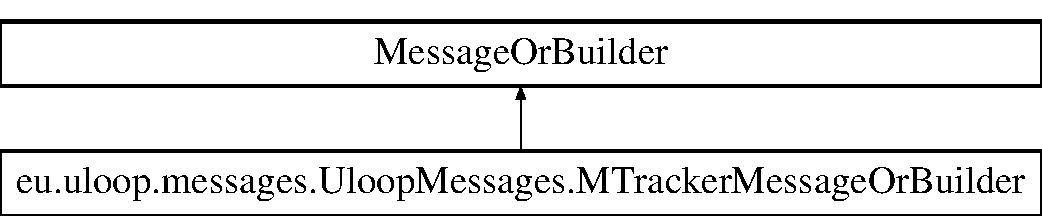
\includegraphics[height=2.000000cm]{interfaceeu_1_1uloop_1_1messages_1_1UloopMessages_1_1MTrackerMessageOrBuilder}
\end{center}
\end{figure}
\subsection*{Public Member Functions}
\begin{DoxyCompactItemize}
\item 
boolean \hyperlink{interfaceeu_1_1uloop_1_1messages_1_1UloopMessages_1_1MTrackerMessageOrBuilder_af2f9c1e18444debe7500fc178aad1ce0}{has\+Time\+For\+Next\+Move} ()
\item 
long \hyperlink{interfaceeu_1_1uloop_1_1messages_1_1UloopMessages_1_1MTrackerMessageOrBuilder_abc9ab5835bd61341f2606c9c43234b50}{get\+Time\+For\+Next\+Move} ()
\item 
boolean \hyperlink{interfaceeu_1_1uloop_1_1messages_1_1UloopMessages_1_1MTrackerMessageOrBuilder_af4d32fde029f9d69b0e04bccbd041fc3}{has\+Current\+Stationary\+Time} ()
\item 
long \hyperlink{interfaceeu_1_1uloop_1_1messages_1_1UloopMessages_1_1MTrackerMessageOrBuilder_a1ad5dcd56e2b665921e99314d591a595}{get\+Current\+Stationary\+Time} ()
\item 
java.\+util.\+List\\*
$<$ eu.\+uloop.\+messages.\+Uloop\+Messages.\+M\+Tracker\+Predicted\+Move $>$ \hyperlink{interfaceeu_1_1uloop_1_1messages_1_1UloopMessages_1_1MTrackerMessageOrBuilder_a0eafcbd9531c7637a40a06e3c16bc69a}{get\+Next\+Gateway\+List\+List} ()
\item 
eu.\+uloop.\+messages.\+Uloop\+Messages.\+M\+Tracker\+Predicted\+Move \hyperlink{interfaceeu_1_1uloop_1_1messages_1_1UloopMessages_1_1MTrackerMessageOrBuilder_aa762ee29bb176bc3aae345eb802ddcff}{get\+Next\+Gateway\+List} (int index)
\item 
int \hyperlink{interfaceeu_1_1uloop_1_1messages_1_1UloopMessages_1_1MTrackerMessageOrBuilder_ab6cd4846488811dba1d7003404d68c1d}{get\+Next\+Gateway\+List\+Count} ()
\item 
java.\+util.\+List$<$?extends \\*
\hyperlink{interfaceeu_1_1uloop_1_1messages_1_1UloopMessages_1_1MTrackerPredictedMoveOrBuilder}{eu.\+uloop.\+messages.\+Uloop\+Messages.\+M\+Tracker\+Predicted\+Move\+Or\+Builder} $>$ \hyperlink{interfaceeu_1_1uloop_1_1messages_1_1UloopMessages_1_1MTrackerMessageOrBuilder_a352dcd71d245033a6caaf574bbd15cf3}{get\+Next\+Gateway\+List\+Or\+Builder\+List} ()
\item 
\hyperlink{interfaceeu_1_1uloop_1_1messages_1_1UloopMessages_1_1MTrackerPredictedMoveOrBuilder}{eu.\+uloop.\+messages.\+Uloop\+Messages.\+M\+Tracker\+Predicted\+Move\+Or\+Builder} \hyperlink{interfaceeu_1_1uloop_1_1messages_1_1UloopMessages_1_1MTrackerMessageOrBuilder_a4142deeb4d926b48e9176a50d75ab871}{get\+Next\+Gateway\+List\+Or\+Builder} (int index)
\end{DoxyCompactItemize}


\subsection{Member Function Documentation}
\hypertarget{interfaceeu_1_1uloop_1_1messages_1_1UloopMessages_1_1MTrackerMessageOrBuilder_a1ad5dcd56e2b665921e99314d591a595}{\index{eu\+::uloop\+::messages\+::\+Uloop\+Messages\+::\+M\+Tracker\+Message\+Or\+Builder@{eu\+::uloop\+::messages\+::\+Uloop\+Messages\+::\+M\+Tracker\+Message\+Or\+Builder}!get\+Current\+Stationary\+Time@{get\+Current\+Stationary\+Time}}
\index{get\+Current\+Stationary\+Time@{get\+Current\+Stationary\+Time}!eu\+::uloop\+::messages\+::\+Uloop\+Messages\+::\+M\+Tracker\+Message\+Or\+Builder@{eu\+::uloop\+::messages\+::\+Uloop\+Messages\+::\+M\+Tracker\+Message\+Or\+Builder}}
\subsubsection[{get\+Current\+Stationary\+Time}]{\setlength{\rightskip}{0pt plus 5cm}long eu.\+uloop.\+messages.\+Uloop\+Messages.\+M\+Tracker\+Message\+Or\+Builder.\+get\+Current\+Stationary\+Time (
\begin{DoxyParamCaption}
{}
\end{DoxyParamCaption}
)}}\label{interfaceeu_1_1uloop_1_1messages_1_1UloopMessages_1_1MTrackerMessageOrBuilder_a1ad5dcd56e2b665921e99314d591a595}
\hypertarget{interfaceeu_1_1uloop_1_1messages_1_1UloopMessages_1_1MTrackerMessageOrBuilder_aa762ee29bb176bc3aae345eb802ddcff}{\index{eu\+::uloop\+::messages\+::\+Uloop\+Messages\+::\+M\+Tracker\+Message\+Or\+Builder@{eu\+::uloop\+::messages\+::\+Uloop\+Messages\+::\+M\+Tracker\+Message\+Or\+Builder}!get\+Next\+Gateway\+List@{get\+Next\+Gateway\+List}}
\index{get\+Next\+Gateway\+List@{get\+Next\+Gateway\+List}!eu\+::uloop\+::messages\+::\+Uloop\+Messages\+::\+M\+Tracker\+Message\+Or\+Builder@{eu\+::uloop\+::messages\+::\+Uloop\+Messages\+::\+M\+Tracker\+Message\+Or\+Builder}}
\subsubsection[{get\+Next\+Gateway\+List}]{\setlength{\rightskip}{0pt plus 5cm}eu.\+uloop.\+messages.\+Uloop\+Messages.\+M\+Tracker\+Predicted\+Move eu.\+uloop.\+messages.\+Uloop\+Messages.\+M\+Tracker\+Message\+Or\+Builder.\+get\+Next\+Gateway\+List (
\begin{DoxyParamCaption}
\item[{int}]{index}
\end{DoxyParamCaption}
)}}\label{interfaceeu_1_1uloop_1_1messages_1_1UloopMessages_1_1MTrackerMessageOrBuilder_aa762ee29bb176bc3aae345eb802ddcff}
\hypertarget{interfaceeu_1_1uloop_1_1messages_1_1UloopMessages_1_1MTrackerMessageOrBuilder_ab6cd4846488811dba1d7003404d68c1d}{\index{eu\+::uloop\+::messages\+::\+Uloop\+Messages\+::\+M\+Tracker\+Message\+Or\+Builder@{eu\+::uloop\+::messages\+::\+Uloop\+Messages\+::\+M\+Tracker\+Message\+Or\+Builder}!get\+Next\+Gateway\+List\+Count@{get\+Next\+Gateway\+List\+Count}}
\index{get\+Next\+Gateway\+List\+Count@{get\+Next\+Gateway\+List\+Count}!eu\+::uloop\+::messages\+::\+Uloop\+Messages\+::\+M\+Tracker\+Message\+Or\+Builder@{eu\+::uloop\+::messages\+::\+Uloop\+Messages\+::\+M\+Tracker\+Message\+Or\+Builder}}
\subsubsection[{get\+Next\+Gateway\+List\+Count}]{\setlength{\rightskip}{0pt plus 5cm}int eu.\+uloop.\+messages.\+Uloop\+Messages.\+M\+Tracker\+Message\+Or\+Builder.\+get\+Next\+Gateway\+List\+Count (
\begin{DoxyParamCaption}
{}
\end{DoxyParamCaption}
)}}\label{interfaceeu_1_1uloop_1_1messages_1_1UloopMessages_1_1MTrackerMessageOrBuilder_ab6cd4846488811dba1d7003404d68c1d}
\hypertarget{interfaceeu_1_1uloop_1_1messages_1_1UloopMessages_1_1MTrackerMessageOrBuilder_a0eafcbd9531c7637a40a06e3c16bc69a}{\index{eu\+::uloop\+::messages\+::\+Uloop\+Messages\+::\+M\+Tracker\+Message\+Or\+Builder@{eu\+::uloop\+::messages\+::\+Uloop\+Messages\+::\+M\+Tracker\+Message\+Or\+Builder}!get\+Next\+Gateway\+List\+List@{get\+Next\+Gateway\+List\+List}}
\index{get\+Next\+Gateway\+List\+List@{get\+Next\+Gateway\+List\+List}!eu\+::uloop\+::messages\+::\+Uloop\+Messages\+::\+M\+Tracker\+Message\+Or\+Builder@{eu\+::uloop\+::messages\+::\+Uloop\+Messages\+::\+M\+Tracker\+Message\+Or\+Builder}}
\subsubsection[{get\+Next\+Gateway\+List\+List}]{\setlength{\rightskip}{0pt plus 5cm}java.\+util.\+List$<$eu.\+uloop.\+messages.\+Uloop\+Messages.\+M\+Tracker\+Predicted\+Move$>$ eu.\+uloop.\+messages.\+Uloop\+Messages.\+M\+Tracker\+Message\+Or\+Builder.\+get\+Next\+Gateway\+List\+List (
\begin{DoxyParamCaption}
{}
\end{DoxyParamCaption}
)}}\label{interfaceeu_1_1uloop_1_1messages_1_1UloopMessages_1_1MTrackerMessageOrBuilder_a0eafcbd9531c7637a40a06e3c16bc69a}
\hypertarget{interfaceeu_1_1uloop_1_1messages_1_1UloopMessages_1_1MTrackerMessageOrBuilder_a4142deeb4d926b48e9176a50d75ab871}{\index{eu\+::uloop\+::messages\+::\+Uloop\+Messages\+::\+M\+Tracker\+Message\+Or\+Builder@{eu\+::uloop\+::messages\+::\+Uloop\+Messages\+::\+M\+Tracker\+Message\+Or\+Builder}!get\+Next\+Gateway\+List\+Or\+Builder@{get\+Next\+Gateway\+List\+Or\+Builder}}
\index{get\+Next\+Gateway\+List\+Or\+Builder@{get\+Next\+Gateway\+List\+Or\+Builder}!eu\+::uloop\+::messages\+::\+Uloop\+Messages\+::\+M\+Tracker\+Message\+Or\+Builder@{eu\+::uloop\+::messages\+::\+Uloop\+Messages\+::\+M\+Tracker\+Message\+Or\+Builder}}
\subsubsection[{get\+Next\+Gateway\+List\+Or\+Builder}]{\setlength{\rightskip}{0pt plus 5cm}{\bf eu.\+uloop.\+messages.\+Uloop\+Messages.\+M\+Tracker\+Predicted\+Move\+Or\+Builder} eu.\+uloop.\+messages.\+Uloop\+Messages.\+M\+Tracker\+Message\+Or\+Builder.\+get\+Next\+Gateway\+List\+Or\+Builder (
\begin{DoxyParamCaption}
\item[{int}]{index}
\end{DoxyParamCaption}
)}}\label{interfaceeu_1_1uloop_1_1messages_1_1UloopMessages_1_1MTrackerMessageOrBuilder_a4142deeb4d926b48e9176a50d75ab871}
\hypertarget{interfaceeu_1_1uloop_1_1messages_1_1UloopMessages_1_1MTrackerMessageOrBuilder_a352dcd71d245033a6caaf574bbd15cf3}{\index{eu\+::uloop\+::messages\+::\+Uloop\+Messages\+::\+M\+Tracker\+Message\+Or\+Builder@{eu\+::uloop\+::messages\+::\+Uloop\+Messages\+::\+M\+Tracker\+Message\+Or\+Builder}!get\+Next\+Gateway\+List\+Or\+Builder\+List@{get\+Next\+Gateway\+List\+Or\+Builder\+List}}
\index{get\+Next\+Gateway\+List\+Or\+Builder\+List@{get\+Next\+Gateway\+List\+Or\+Builder\+List}!eu\+::uloop\+::messages\+::\+Uloop\+Messages\+::\+M\+Tracker\+Message\+Or\+Builder@{eu\+::uloop\+::messages\+::\+Uloop\+Messages\+::\+M\+Tracker\+Message\+Or\+Builder}}
\subsubsection[{get\+Next\+Gateway\+List\+Or\+Builder\+List}]{\setlength{\rightskip}{0pt plus 5cm}java.\+util.\+List$<$? extends {\bf eu.\+uloop.\+messages.\+Uloop\+Messages.\+M\+Tracker\+Predicted\+Move\+Or\+Builder}$>$ eu.\+uloop.\+messages.\+Uloop\+Messages.\+M\+Tracker\+Message\+Or\+Builder.\+get\+Next\+Gateway\+List\+Or\+Builder\+List (
\begin{DoxyParamCaption}
{}
\end{DoxyParamCaption}
)}}\label{interfaceeu_1_1uloop_1_1messages_1_1UloopMessages_1_1MTrackerMessageOrBuilder_a352dcd71d245033a6caaf574bbd15cf3}
\hypertarget{interfaceeu_1_1uloop_1_1messages_1_1UloopMessages_1_1MTrackerMessageOrBuilder_abc9ab5835bd61341f2606c9c43234b50}{\index{eu\+::uloop\+::messages\+::\+Uloop\+Messages\+::\+M\+Tracker\+Message\+Or\+Builder@{eu\+::uloop\+::messages\+::\+Uloop\+Messages\+::\+M\+Tracker\+Message\+Or\+Builder}!get\+Time\+For\+Next\+Move@{get\+Time\+For\+Next\+Move}}
\index{get\+Time\+For\+Next\+Move@{get\+Time\+For\+Next\+Move}!eu\+::uloop\+::messages\+::\+Uloop\+Messages\+::\+M\+Tracker\+Message\+Or\+Builder@{eu\+::uloop\+::messages\+::\+Uloop\+Messages\+::\+M\+Tracker\+Message\+Or\+Builder}}
\subsubsection[{get\+Time\+For\+Next\+Move}]{\setlength{\rightskip}{0pt plus 5cm}long eu.\+uloop.\+messages.\+Uloop\+Messages.\+M\+Tracker\+Message\+Or\+Builder.\+get\+Time\+For\+Next\+Move (
\begin{DoxyParamCaption}
{}
\end{DoxyParamCaption}
)}}\label{interfaceeu_1_1uloop_1_1messages_1_1UloopMessages_1_1MTrackerMessageOrBuilder_abc9ab5835bd61341f2606c9c43234b50}
\hypertarget{interfaceeu_1_1uloop_1_1messages_1_1UloopMessages_1_1MTrackerMessageOrBuilder_af4d32fde029f9d69b0e04bccbd041fc3}{\index{eu\+::uloop\+::messages\+::\+Uloop\+Messages\+::\+M\+Tracker\+Message\+Or\+Builder@{eu\+::uloop\+::messages\+::\+Uloop\+Messages\+::\+M\+Tracker\+Message\+Or\+Builder}!has\+Current\+Stationary\+Time@{has\+Current\+Stationary\+Time}}
\index{has\+Current\+Stationary\+Time@{has\+Current\+Stationary\+Time}!eu\+::uloop\+::messages\+::\+Uloop\+Messages\+::\+M\+Tracker\+Message\+Or\+Builder@{eu\+::uloop\+::messages\+::\+Uloop\+Messages\+::\+M\+Tracker\+Message\+Or\+Builder}}
\subsubsection[{has\+Current\+Stationary\+Time}]{\setlength{\rightskip}{0pt plus 5cm}boolean eu.\+uloop.\+messages.\+Uloop\+Messages.\+M\+Tracker\+Message\+Or\+Builder.\+has\+Current\+Stationary\+Time (
\begin{DoxyParamCaption}
{}
\end{DoxyParamCaption}
)}}\label{interfaceeu_1_1uloop_1_1messages_1_1UloopMessages_1_1MTrackerMessageOrBuilder_af4d32fde029f9d69b0e04bccbd041fc3}
\hypertarget{interfaceeu_1_1uloop_1_1messages_1_1UloopMessages_1_1MTrackerMessageOrBuilder_af2f9c1e18444debe7500fc178aad1ce0}{\index{eu\+::uloop\+::messages\+::\+Uloop\+Messages\+::\+M\+Tracker\+Message\+Or\+Builder@{eu\+::uloop\+::messages\+::\+Uloop\+Messages\+::\+M\+Tracker\+Message\+Or\+Builder}!has\+Time\+For\+Next\+Move@{has\+Time\+For\+Next\+Move}}
\index{has\+Time\+For\+Next\+Move@{has\+Time\+For\+Next\+Move}!eu\+::uloop\+::messages\+::\+Uloop\+Messages\+::\+M\+Tracker\+Message\+Or\+Builder@{eu\+::uloop\+::messages\+::\+Uloop\+Messages\+::\+M\+Tracker\+Message\+Or\+Builder}}
\subsubsection[{has\+Time\+For\+Next\+Move}]{\setlength{\rightskip}{0pt plus 5cm}boolean eu.\+uloop.\+messages.\+Uloop\+Messages.\+M\+Tracker\+Message\+Or\+Builder.\+has\+Time\+For\+Next\+Move (
\begin{DoxyParamCaption}
{}
\end{DoxyParamCaption}
)}}\label{interfaceeu_1_1uloop_1_1messages_1_1UloopMessages_1_1MTrackerMessageOrBuilder_af2f9c1e18444debe7500fc178aad1ce0}


The documentation for this interface was generated from the following file\+:\begin{DoxyCompactItemize}
\item 
src/eu/uloop/messages/\hyperlink{UloopMessages_8java}{Uloop\+Messages.\+java}\end{DoxyCompactItemize}

\hypertarget{classlib_1_1api_1_1UloopMTrackerMessage_1_1MTrackerPredictedM}{\section{lib.\+api.\+Uloop\+M\+Tracker\+Message.\+M\+Tracker\+Predicted\+M Class Reference}
\label{classlib_1_1api_1_1UloopMTrackerMessage_1_1MTrackerPredictedM}\index{lib.\+api.\+Uloop\+M\+Tracker\+Message.\+M\+Tracker\+Predicted\+M@{lib.\+api.\+Uloop\+M\+Tracker\+Message.\+M\+Tracker\+Predicted\+M}}
}
\subsection*{Public Member Functions}
\begin{DoxyCompactItemize}
\item 
void \hyperlink{classlib_1_1api_1_1UloopMTrackerMessage_1_1MTrackerPredictedM_a1c29c9403594c82d8564b2d63daf3bb2}{set\+B\+S\+S\+I\+D} (String bssid)
\item 
void \hyperlink{classlib_1_1api_1_1UloopMTrackerMessage_1_1MTrackerPredictedM_a70f81c2f1461a7b1232fc5fa41d18d62}{setstationary\+Time} (long time)
\item 
void \hyperlink{classlib_1_1api_1_1UloopMTrackerMessage_1_1MTrackerPredictedM_a2ef3674678bd15d7876af605bc73203f}{set\+Last\+Gatewat\+I\+P} (String gateip)
\end{DoxyCompactItemize}
\subsection*{Private Attributes}
\begin{DoxyCompactItemize}
\item 
String \hyperlink{classlib_1_1api_1_1UloopMTrackerMessage_1_1MTrackerPredictedM_ae63f95b7e7df89f62422c2d54683b1fc}{B\+S\+S\+I\+D}
\item 
long \hyperlink{classlib_1_1api_1_1UloopMTrackerMessage_1_1MTrackerPredictedM_a6fc77030c0afaee3814665d12815c532}{stationary\+Time}
\item 
String \hyperlink{classlib_1_1api_1_1UloopMTrackerMessage_1_1MTrackerPredictedM_a6b0813739dddddbec4008aff77f9c7fd}{last\+Gateway\+I\+P}
\end{DoxyCompactItemize}


\subsection{Member Function Documentation}
\hypertarget{classlib_1_1api_1_1UloopMTrackerMessage_1_1MTrackerPredictedM_a1c29c9403594c82d8564b2d63daf3bb2}{\index{lib\+::api\+::\+Uloop\+M\+Tracker\+Message\+::\+M\+Tracker\+Predicted\+M@{lib\+::api\+::\+Uloop\+M\+Tracker\+Message\+::\+M\+Tracker\+Predicted\+M}!set\+B\+S\+S\+I\+D@{set\+B\+S\+S\+I\+D}}
\index{set\+B\+S\+S\+I\+D@{set\+B\+S\+S\+I\+D}!lib\+::api\+::\+Uloop\+M\+Tracker\+Message\+::\+M\+Tracker\+Predicted\+M@{lib\+::api\+::\+Uloop\+M\+Tracker\+Message\+::\+M\+Tracker\+Predicted\+M}}
\subsubsection[{set\+B\+S\+S\+I\+D}]{\setlength{\rightskip}{0pt plus 5cm}void lib.\+api.\+Uloop\+M\+Tracker\+Message.\+M\+Tracker\+Predicted\+M.\+set\+B\+S\+S\+I\+D (
\begin{DoxyParamCaption}
\item[{String}]{bssid}
\end{DoxyParamCaption}
)}}\label{classlib_1_1api_1_1UloopMTrackerMessage_1_1MTrackerPredictedM_a1c29c9403594c82d8564b2d63daf3bb2}
\hypertarget{classlib_1_1api_1_1UloopMTrackerMessage_1_1MTrackerPredictedM_a2ef3674678bd15d7876af605bc73203f}{\index{lib\+::api\+::\+Uloop\+M\+Tracker\+Message\+::\+M\+Tracker\+Predicted\+M@{lib\+::api\+::\+Uloop\+M\+Tracker\+Message\+::\+M\+Tracker\+Predicted\+M}!set\+Last\+Gatewat\+I\+P@{set\+Last\+Gatewat\+I\+P}}
\index{set\+Last\+Gatewat\+I\+P@{set\+Last\+Gatewat\+I\+P}!lib\+::api\+::\+Uloop\+M\+Tracker\+Message\+::\+M\+Tracker\+Predicted\+M@{lib\+::api\+::\+Uloop\+M\+Tracker\+Message\+::\+M\+Tracker\+Predicted\+M}}
\subsubsection[{set\+Last\+Gatewat\+I\+P}]{\setlength{\rightskip}{0pt plus 5cm}void lib.\+api.\+Uloop\+M\+Tracker\+Message.\+M\+Tracker\+Predicted\+M.\+set\+Last\+Gatewat\+I\+P (
\begin{DoxyParamCaption}
\item[{String}]{gateip}
\end{DoxyParamCaption}
)}}\label{classlib_1_1api_1_1UloopMTrackerMessage_1_1MTrackerPredictedM_a2ef3674678bd15d7876af605bc73203f}
\hypertarget{classlib_1_1api_1_1UloopMTrackerMessage_1_1MTrackerPredictedM_a70f81c2f1461a7b1232fc5fa41d18d62}{\index{lib\+::api\+::\+Uloop\+M\+Tracker\+Message\+::\+M\+Tracker\+Predicted\+M@{lib\+::api\+::\+Uloop\+M\+Tracker\+Message\+::\+M\+Tracker\+Predicted\+M}!setstationary\+Time@{setstationary\+Time}}
\index{setstationary\+Time@{setstationary\+Time}!lib\+::api\+::\+Uloop\+M\+Tracker\+Message\+::\+M\+Tracker\+Predicted\+M@{lib\+::api\+::\+Uloop\+M\+Tracker\+Message\+::\+M\+Tracker\+Predicted\+M}}
\subsubsection[{setstationary\+Time}]{\setlength{\rightskip}{0pt plus 5cm}void lib.\+api.\+Uloop\+M\+Tracker\+Message.\+M\+Tracker\+Predicted\+M.\+setstationary\+Time (
\begin{DoxyParamCaption}
\item[{long}]{time}
\end{DoxyParamCaption}
)}}\label{classlib_1_1api_1_1UloopMTrackerMessage_1_1MTrackerPredictedM_a70f81c2f1461a7b1232fc5fa41d18d62}


\subsection{Member Data Documentation}
\hypertarget{classlib_1_1api_1_1UloopMTrackerMessage_1_1MTrackerPredictedM_ae63f95b7e7df89f62422c2d54683b1fc}{\index{lib\+::api\+::\+Uloop\+M\+Tracker\+Message\+::\+M\+Tracker\+Predicted\+M@{lib\+::api\+::\+Uloop\+M\+Tracker\+Message\+::\+M\+Tracker\+Predicted\+M}!B\+S\+S\+I\+D@{B\+S\+S\+I\+D}}
\index{B\+S\+S\+I\+D@{B\+S\+S\+I\+D}!lib\+::api\+::\+Uloop\+M\+Tracker\+Message\+::\+M\+Tracker\+Predicted\+M@{lib\+::api\+::\+Uloop\+M\+Tracker\+Message\+::\+M\+Tracker\+Predicted\+M}}
\subsubsection[{B\+S\+S\+I\+D}]{\setlength{\rightskip}{0pt plus 5cm}String lib.\+api.\+Uloop\+M\+Tracker\+Message.\+M\+Tracker\+Predicted\+M.\+B\+S\+S\+I\+D\hspace{0.3cm}{\ttfamily [private]}}}\label{classlib_1_1api_1_1UloopMTrackerMessage_1_1MTrackerPredictedM_ae63f95b7e7df89f62422c2d54683b1fc}
\hypertarget{classlib_1_1api_1_1UloopMTrackerMessage_1_1MTrackerPredictedM_a6b0813739dddddbec4008aff77f9c7fd}{\index{lib\+::api\+::\+Uloop\+M\+Tracker\+Message\+::\+M\+Tracker\+Predicted\+M@{lib\+::api\+::\+Uloop\+M\+Tracker\+Message\+::\+M\+Tracker\+Predicted\+M}!last\+Gateway\+I\+P@{last\+Gateway\+I\+P}}
\index{last\+Gateway\+I\+P@{last\+Gateway\+I\+P}!lib\+::api\+::\+Uloop\+M\+Tracker\+Message\+::\+M\+Tracker\+Predicted\+M@{lib\+::api\+::\+Uloop\+M\+Tracker\+Message\+::\+M\+Tracker\+Predicted\+M}}
\subsubsection[{last\+Gateway\+I\+P}]{\setlength{\rightskip}{0pt plus 5cm}String lib.\+api.\+Uloop\+M\+Tracker\+Message.\+M\+Tracker\+Predicted\+M.\+last\+Gateway\+I\+P\hspace{0.3cm}{\ttfamily [private]}}}\label{classlib_1_1api_1_1UloopMTrackerMessage_1_1MTrackerPredictedM_a6b0813739dddddbec4008aff77f9c7fd}
\hypertarget{classlib_1_1api_1_1UloopMTrackerMessage_1_1MTrackerPredictedM_a6fc77030c0afaee3814665d12815c532}{\index{lib\+::api\+::\+Uloop\+M\+Tracker\+Message\+::\+M\+Tracker\+Predicted\+M@{lib\+::api\+::\+Uloop\+M\+Tracker\+Message\+::\+M\+Tracker\+Predicted\+M}!stationary\+Time@{stationary\+Time}}
\index{stationary\+Time@{stationary\+Time}!lib\+::api\+::\+Uloop\+M\+Tracker\+Message\+::\+M\+Tracker\+Predicted\+M@{lib\+::api\+::\+Uloop\+M\+Tracker\+Message\+::\+M\+Tracker\+Predicted\+M}}
\subsubsection[{stationary\+Time}]{\setlength{\rightskip}{0pt plus 5cm}long lib.\+api.\+Uloop\+M\+Tracker\+Message.\+M\+Tracker\+Predicted\+M.\+stationary\+Time\hspace{0.3cm}{\ttfamily [private]}}}\label{classlib_1_1api_1_1UloopMTrackerMessage_1_1MTrackerPredictedM_a6fc77030c0afaee3814665d12815c532}


The documentation for this class was generated from the following file\+:\begin{DoxyCompactItemize}
\item 
src/lib/api/\hyperlink{UloopMTrackerMessage_8java}{Uloop\+M\+Tracker\+Message.\+java}\end{DoxyCompactItemize}

\hypertarget{interfaceeu_1_1uloop_1_1messages_1_1UloopMessages_1_1MTrackerPredictedMoveOrBuilder}{\section{eu.\+uloop.\+messages.\+Uloop\+Messages.\+M\+Tracker\+Predicted\+Move\+Or\+Builder Interface Reference}
\label{interfaceeu_1_1uloop_1_1messages_1_1UloopMessages_1_1MTrackerPredictedMoveOrBuilder}\index{eu.\+uloop.\+messages.\+Uloop\+Messages.\+M\+Tracker\+Predicted\+Move\+Or\+Builder@{eu.\+uloop.\+messages.\+Uloop\+Messages.\+M\+Tracker\+Predicted\+Move\+Or\+Builder}}
}
Inheritance diagram for eu.\+uloop.\+messages.\+Uloop\+Messages.\+M\+Tracker\+Predicted\+Move\+Or\+Builder\+:\begin{figure}[H]
\begin{center}
\leavevmode
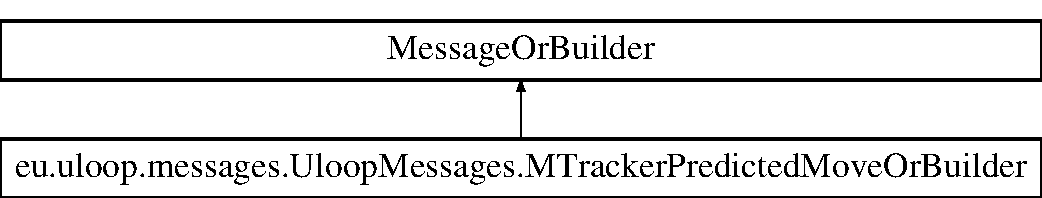
\includegraphics[height=2.000000cm]{interfaceeu_1_1uloop_1_1messages_1_1UloopMessages_1_1MTrackerPredictedMoveOrBuilder}
\end{center}
\end{figure}
\subsection*{Public Member Functions}
\begin{DoxyCompactItemize}
\item 
boolean \hyperlink{interfaceeu_1_1uloop_1_1messages_1_1UloopMessages_1_1MTrackerPredictedMoveOrBuilder_a539b8efaf7536dba5fcf80e3de474142}{has\+B\+S\+S\+I\+D} ()
\item 
String \hyperlink{interfaceeu_1_1uloop_1_1messages_1_1UloopMessages_1_1MTrackerPredictedMoveOrBuilder_aa8aeb65f1118f2451a7176df6e62af51}{get\+B\+S\+S\+I\+D} ()
\item 
boolean \hyperlink{interfaceeu_1_1uloop_1_1messages_1_1UloopMessages_1_1MTrackerPredictedMoveOrBuilder_a07c2f90c6dc487a62606d544268b220e}{has\+Stationary\+Time} ()
\item 
long \hyperlink{interfaceeu_1_1uloop_1_1messages_1_1UloopMessages_1_1MTrackerPredictedMoveOrBuilder_a5e97562378bb85f029691b5c7e882f8e}{get\+Stationary\+Time} ()
\item 
boolean \hyperlink{interfaceeu_1_1uloop_1_1messages_1_1UloopMessages_1_1MTrackerPredictedMoveOrBuilder_aa7aa3a7e78eb917f85b1dd561f61aaf9}{has\+Last\+Gateway\+I\+P} ()
\item 
String \hyperlink{interfaceeu_1_1uloop_1_1messages_1_1UloopMessages_1_1MTrackerPredictedMoveOrBuilder_a516bad81ba3e850050d02ff1cae42da7}{get\+Last\+Gateway\+I\+P} ()
\end{DoxyCompactItemize}


\subsection{Member Function Documentation}
\hypertarget{interfaceeu_1_1uloop_1_1messages_1_1UloopMessages_1_1MTrackerPredictedMoveOrBuilder_aa8aeb65f1118f2451a7176df6e62af51}{\index{eu\+::uloop\+::messages\+::\+Uloop\+Messages\+::\+M\+Tracker\+Predicted\+Move\+Or\+Builder@{eu\+::uloop\+::messages\+::\+Uloop\+Messages\+::\+M\+Tracker\+Predicted\+Move\+Or\+Builder}!get\+B\+S\+S\+I\+D@{get\+B\+S\+S\+I\+D}}
\index{get\+B\+S\+S\+I\+D@{get\+B\+S\+S\+I\+D}!eu\+::uloop\+::messages\+::\+Uloop\+Messages\+::\+M\+Tracker\+Predicted\+Move\+Or\+Builder@{eu\+::uloop\+::messages\+::\+Uloop\+Messages\+::\+M\+Tracker\+Predicted\+Move\+Or\+Builder}}
\subsubsection[{get\+B\+S\+S\+I\+D}]{\setlength{\rightskip}{0pt plus 5cm}String eu.\+uloop.\+messages.\+Uloop\+Messages.\+M\+Tracker\+Predicted\+Move\+Or\+Builder.\+get\+B\+S\+S\+I\+D (
\begin{DoxyParamCaption}
{}
\end{DoxyParamCaption}
)}}\label{interfaceeu_1_1uloop_1_1messages_1_1UloopMessages_1_1MTrackerPredictedMoveOrBuilder_aa8aeb65f1118f2451a7176df6e62af51}
\hypertarget{interfaceeu_1_1uloop_1_1messages_1_1UloopMessages_1_1MTrackerPredictedMoveOrBuilder_a516bad81ba3e850050d02ff1cae42da7}{\index{eu\+::uloop\+::messages\+::\+Uloop\+Messages\+::\+M\+Tracker\+Predicted\+Move\+Or\+Builder@{eu\+::uloop\+::messages\+::\+Uloop\+Messages\+::\+M\+Tracker\+Predicted\+Move\+Or\+Builder}!get\+Last\+Gateway\+I\+P@{get\+Last\+Gateway\+I\+P}}
\index{get\+Last\+Gateway\+I\+P@{get\+Last\+Gateway\+I\+P}!eu\+::uloop\+::messages\+::\+Uloop\+Messages\+::\+M\+Tracker\+Predicted\+Move\+Or\+Builder@{eu\+::uloop\+::messages\+::\+Uloop\+Messages\+::\+M\+Tracker\+Predicted\+Move\+Or\+Builder}}
\subsubsection[{get\+Last\+Gateway\+I\+P}]{\setlength{\rightskip}{0pt plus 5cm}String eu.\+uloop.\+messages.\+Uloop\+Messages.\+M\+Tracker\+Predicted\+Move\+Or\+Builder.\+get\+Last\+Gateway\+I\+P (
\begin{DoxyParamCaption}
{}
\end{DoxyParamCaption}
)}}\label{interfaceeu_1_1uloop_1_1messages_1_1UloopMessages_1_1MTrackerPredictedMoveOrBuilder_a516bad81ba3e850050d02ff1cae42da7}
\hypertarget{interfaceeu_1_1uloop_1_1messages_1_1UloopMessages_1_1MTrackerPredictedMoveOrBuilder_a5e97562378bb85f029691b5c7e882f8e}{\index{eu\+::uloop\+::messages\+::\+Uloop\+Messages\+::\+M\+Tracker\+Predicted\+Move\+Or\+Builder@{eu\+::uloop\+::messages\+::\+Uloop\+Messages\+::\+M\+Tracker\+Predicted\+Move\+Or\+Builder}!get\+Stationary\+Time@{get\+Stationary\+Time}}
\index{get\+Stationary\+Time@{get\+Stationary\+Time}!eu\+::uloop\+::messages\+::\+Uloop\+Messages\+::\+M\+Tracker\+Predicted\+Move\+Or\+Builder@{eu\+::uloop\+::messages\+::\+Uloop\+Messages\+::\+M\+Tracker\+Predicted\+Move\+Or\+Builder}}
\subsubsection[{get\+Stationary\+Time}]{\setlength{\rightskip}{0pt plus 5cm}long eu.\+uloop.\+messages.\+Uloop\+Messages.\+M\+Tracker\+Predicted\+Move\+Or\+Builder.\+get\+Stationary\+Time (
\begin{DoxyParamCaption}
{}
\end{DoxyParamCaption}
)}}\label{interfaceeu_1_1uloop_1_1messages_1_1UloopMessages_1_1MTrackerPredictedMoveOrBuilder_a5e97562378bb85f029691b5c7e882f8e}
\hypertarget{interfaceeu_1_1uloop_1_1messages_1_1UloopMessages_1_1MTrackerPredictedMoveOrBuilder_a539b8efaf7536dba5fcf80e3de474142}{\index{eu\+::uloop\+::messages\+::\+Uloop\+Messages\+::\+M\+Tracker\+Predicted\+Move\+Or\+Builder@{eu\+::uloop\+::messages\+::\+Uloop\+Messages\+::\+M\+Tracker\+Predicted\+Move\+Or\+Builder}!has\+B\+S\+S\+I\+D@{has\+B\+S\+S\+I\+D}}
\index{has\+B\+S\+S\+I\+D@{has\+B\+S\+S\+I\+D}!eu\+::uloop\+::messages\+::\+Uloop\+Messages\+::\+M\+Tracker\+Predicted\+Move\+Or\+Builder@{eu\+::uloop\+::messages\+::\+Uloop\+Messages\+::\+M\+Tracker\+Predicted\+Move\+Or\+Builder}}
\subsubsection[{has\+B\+S\+S\+I\+D}]{\setlength{\rightskip}{0pt plus 5cm}boolean eu.\+uloop.\+messages.\+Uloop\+Messages.\+M\+Tracker\+Predicted\+Move\+Or\+Builder.\+has\+B\+S\+S\+I\+D (
\begin{DoxyParamCaption}
{}
\end{DoxyParamCaption}
)}}\label{interfaceeu_1_1uloop_1_1messages_1_1UloopMessages_1_1MTrackerPredictedMoveOrBuilder_a539b8efaf7536dba5fcf80e3de474142}
\hypertarget{interfaceeu_1_1uloop_1_1messages_1_1UloopMessages_1_1MTrackerPredictedMoveOrBuilder_aa7aa3a7e78eb917f85b1dd561f61aaf9}{\index{eu\+::uloop\+::messages\+::\+Uloop\+Messages\+::\+M\+Tracker\+Predicted\+Move\+Or\+Builder@{eu\+::uloop\+::messages\+::\+Uloop\+Messages\+::\+M\+Tracker\+Predicted\+Move\+Or\+Builder}!has\+Last\+Gateway\+I\+P@{has\+Last\+Gateway\+I\+P}}
\index{has\+Last\+Gateway\+I\+P@{has\+Last\+Gateway\+I\+P}!eu\+::uloop\+::messages\+::\+Uloop\+Messages\+::\+M\+Tracker\+Predicted\+Move\+Or\+Builder@{eu\+::uloop\+::messages\+::\+Uloop\+Messages\+::\+M\+Tracker\+Predicted\+Move\+Or\+Builder}}
\subsubsection[{has\+Last\+Gateway\+I\+P}]{\setlength{\rightskip}{0pt plus 5cm}boolean eu.\+uloop.\+messages.\+Uloop\+Messages.\+M\+Tracker\+Predicted\+Move\+Or\+Builder.\+has\+Last\+Gateway\+I\+P (
\begin{DoxyParamCaption}
{}
\end{DoxyParamCaption}
)}}\label{interfaceeu_1_1uloop_1_1messages_1_1UloopMessages_1_1MTrackerPredictedMoveOrBuilder_aa7aa3a7e78eb917f85b1dd561f61aaf9}
\hypertarget{interfaceeu_1_1uloop_1_1messages_1_1UloopMessages_1_1MTrackerPredictedMoveOrBuilder_a07c2f90c6dc487a62606d544268b220e}{\index{eu\+::uloop\+::messages\+::\+Uloop\+Messages\+::\+M\+Tracker\+Predicted\+Move\+Or\+Builder@{eu\+::uloop\+::messages\+::\+Uloop\+Messages\+::\+M\+Tracker\+Predicted\+Move\+Or\+Builder}!has\+Stationary\+Time@{has\+Stationary\+Time}}
\index{has\+Stationary\+Time@{has\+Stationary\+Time}!eu\+::uloop\+::messages\+::\+Uloop\+Messages\+::\+M\+Tracker\+Predicted\+Move\+Or\+Builder@{eu\+::uloop\+::messages\+::\+Uloop\+Messages\+::\+M\+Tracker\+Predicted\+Move\+Or\+Builder}}
\subsubsection[{has\+Stationary\+Time}]{\setlength{\rightskip}{0pt plus 5cm}boolean eu.\+uloop.\+messages.\+Uloop\+Messages.\+M\+Tracker\+Predicted\+Move\+Or\+Builder.\+has\+Stationary\+Time (
\begin{DoxyParamCaption}
{}
\end{DoxyParamCaption}
)}}\label{interfaceeu_1_1uloop_1_1messages_1_1UloopMessages_1_1MTrackerPredictedMoveOrBuilder_a07c2f90c6dc487a62606d544268b220e}


The documentation for this interface was generated from the following file\+:\begin{DoxyCompactItemize}
\item 
src/eu/uloop/messages/\hyperlink{UloopMessages_8java}{Uloop\+Messages.\+java}\end{DoxyCompactItemize}

\hypertarget{classeu_1_1uloop_1_1mobilitytracker_1_1MTrackerService}{\section{eu.\+uloop.\+mobilitytracker.\+M\+Tracker\+Service Class Reference}
\label{classeu_1_1uloop_1_1mobilitytracker_1_1MTrackerService}\index{eu.\+uloop.\+mobilitytracker.\+M\+Tracker\+Service@{eu.\+uloop.\+mobilitytracker.\+M\+Tracker\+Service}}
}
Inheritance diagram for eu.\+uloop.\+mobilitytracker.\+M\+Tracker\+Service\+:\begin{figure}[H]
\begin{center}
\leavevmode
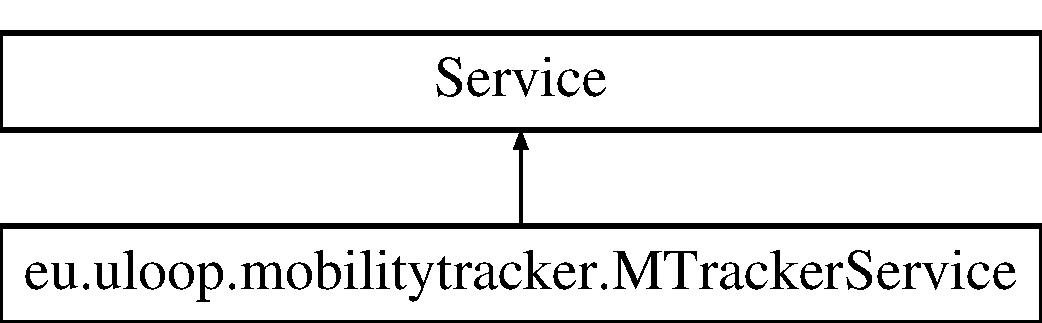
\includegraphics[height=2.000000cm]{classeu_1_1uloop_1_1mobilitytracker_1_1MTrackerService}
\end{center}
\end{figure}
\subsection*{Classes}
\begin{DoxyCompactItemize}
\item 
class \hyperlink{classeu_1_1uloop_1_1mobilitytracker_1_1MTrackerService_1_1LocalBinder}{Local\+Binder}
\item 
class {\bfseries M\+Tracker\+Service\+Wifi\+Listener}
\item 
class \hyperlink{classeu_1_1uloop_1_1mobilitytracker_1_1MTrackerService_1_1SendInformationWithGatewayTask}{Send\+Information\+With\+Gateway\+Task}
\end{DoxyCompactItemize}
\subsection*{Public Member Functions}
\begin{DoxyCompactItemize}
\item 
void \hyperlink{classeu_1_1uloop_1_1mobilitytracker_1_1MTrackerService_a770db9d563bd7c56b2950fc50786832c}{start\+Periodic\+Scanning} ()
\item 
void \hyperlink{classeu_1_1uloop_1_1mobilitytracker_1_1MTrackerService_a046b54f3843bc8aceb2bf9869d103918}{stop\+Periodic\+Scanning} ()
\item 
void \hyperlink{classeu_1_1uloop_1_1mobilitytracker_1_1MTrackerService_aad15cdef47d25b7dad3f2fc13254bf15}{on\+Create} ()
\item 
int \hyperlink{classeu_1_1uloop_1_1mobilitytracker_1_1MTrackerService_a65dde672e32aaec79b26219c2f179643}{on\+Start\+Command} (Intent intent, int flags, int start\+Id)
\item 
void \hyperlink{classeu_1_1uloop_1_1mobilitytracker_1_1MTrackerService_a60a7047b1633b7809af6e69beb420c40}{on\+Destroy} ()
\item 
I\+Binder \hyperlink{classeu_1_1uloop_1_1mobilitytracker_1_1MTrackerService_a24bdd6039581d524211d4f4d92adb70e}{on\+Bind} (Intent intent)
\item 
void \hyperlink{classeu_1_1uloop_1_1mobilitytracker_1_1MTrackerService_a5332e648f938ae1255c4b12aa0d82054}{set\+On\+State\+Change\+Listener} (\hyperlink{interfaceeu_1_1uloop_1_1mobilitytracker_1_1DataBaseChangeListener}{Data\+Base\+Change\+Listener} listener)
\item 
void \hyperlink{classeu_1_1uloop_1_1mobilitytracker_1_1MTrackerService_a5f1b2bb03919db654a59d69681a575e7}{clear\+On\+State\+Change\+Listeners} ()
\item 
void \hyperlink{classeu_1_1uloop_1_1mobilitytracker_1_1MTrackerService_a494c3da30f037844d0636ba505e8b40f}{write\+A\+P\+List\+To\+File} ()
\item 
void \hyperlink{classeu_1_1uloop_1_1mobilitytracker_1_1MTrackerService_a9688b6a2da0c9e673d4a71e261b6496b}{write\+Visit\+List\+To\+File} ()
\item 
boolean \hyperlink{classeu_1_1uloop_1_1mobilitytracker_1_1MTrackerService_a437ec1fb6cdc9b80f09afb76508f74fc}{set\+Uloop\+Dispositional\+Trust} (double uloop\+D\+T)
\end{DoxyCompactItemize}
\subsection*{Protected Member Functions}
\begin{DoxyCompactItemize}
\item 
List$<$ \hyperlink{classeu_1_1uloop_1_1mobilitytracker_1_1MTrackerAP}{M\+Tracker\+A\+P} $>$ \hyperlink{classeu_1_1uloop_1_1mobilitytracker_1_1MTrackerService_ace7c25f76f1ec7b2cfc4e5a4b28f68e9}{get\+Data} ()
\end{DoxyCompactItemize}
\subsection*{Private Member Functions}
\begin{DoxyCompactItemize}
\item 
void \hyperlink{classeu_1_1uloop_1_1mobilitytracker_1_1MTrackerService_a3d1e08686bc3b88de0b5f5d777a31f5c}{notify\+Data\+Base\+Change} ()
\item 
void \hyperlink{classeu_1_1uloop_1_1mobilitytracker_1_1MTrackerService_abd897fb99831f3214a31ba4656b012c5}{notify\+Predicted\+Move\+Change} (String new\+Message)
\item 
void \hyperlink{classeu_1_1uloop_1_1mobilitytracker_1_1MTrackerService_a10277606556c2a61d4486184829be9d5}{announce\+Possible\+Handover} (String next\+Bssid, String next\+Last\+Gateway\+Ip, long next\+Stationary\+Time, long timeto\+Move, long current\+Stationary\+Time)
\end{DoxyCompactItemize}
\subsection*{Private Attributes}
\begin{DoxyCompactItemize}
\item 
double \hyperlink{classeu_1_1uloop_1_1mobilitytracker_1_1MTrackerService_aefb00b5f991cff950571c5f672887fc9}{uloop\+Dispositional\+Trust} = 1.\+0
\item 
\hyperlink{classeu_1_1uloop_1_1mobilitytracker_1_1MTrackerWifiManager}{M\+Tracker\+Wifi\+Manager} \hyperlink{classeu_1_1uloop_1_1mobilitytracker_1_1MTrackerService_aecb42f35385576caa82ce620bf9cd18f}{wifi\+Manager}
\item 
M\+Tracker\+Service\+Wifi\+Listener \hyperlink{classeu_1_1uloop_1_1mobilitytracker_1_1MTrackerService_a753348851dbd47cb52c5b3e22c2528fe}{wifi\+Listener}
\item 
Array\+List$<$ \hyperlink{interfaceeu_1_1uloop_1_1mobilitytracker_1_1DataBaseChangeListener}{Data\+Base\+Change\+Listener} $>$ \hyperlink{classeu_1_1uloop_1_1mobilitytracker_1_1MTrackerService_a204aaa3e3f75b5783a0a4e4c49b8842e}{listeners} = new Array\+List$<$\hyperlink{interfaceeu_1_1uloop_1_1mobilitytracker_1_1DataBaseChangeListener}{Data\+Base\+Change\+Listener}$>$ ()
\item 
final I\+Binder \hyperlink{classeu_1_1uloop_1_1mobilitytracker_1_1MTrackerService_a7d8d344f0b2cfe0ebb5ab619dfdbecbb}{m\+Binder} = new \hyperlink{classeu_1_1uloop_1_1mobilitytracker_1_1MTrackerService_1_1LocalBinder}{Local\+Binder}()
\end{DoxyCompactItemize}


\subsection{Detailed Description}
This class is contains the core functionalities of the application. The \hyperlink{classeu_1_1uloop_1_1mobilitytracker_1_1MTrackerService}{M\+Tracker\+Service} will run in background, getting W\+I-\/\+F\+I parameters and storing the required information in the database.

\begin{DoxyAuthor}{Author}
Jonnahtan Saltarin (U\+L\+H\+T) 

Rute Sofia (U\+L\+H\+T) 

Christian da Silva Pereira (U\+L\+H\+T) 

Luis Amaral Lopes (U\+L\+H\+T)
\end{DoxyAuthor}
\begin{DoxyVersion}{Version}
3.\+0 
\end{DoxyVersion}


\subsection{Member Function Documentation}
\hypertarget{classeu_1_1uloop_1_1mobilitytracker_1_1MTrackerService_a10277606556c2a61d4486184829be9d5}{\index{eu\+::uloop\+::mobilitytracker\+::\+M\+Tracker\+Service@{eu\+::uloop\+::mobilitytracker\+::\+M\+Tracker\+Service}!announce\+Possible\+Handover@{announce\+Possible\+Handover}}
\index{announce\+Possible\+Handover@{announce\+Possible\+Handover}!eu\+::uloop\+::mobilitytracker\+::\+M\+Tracker\+Service@{eu\+::uloop\+::mobilitytracker\+::\+M\+Tracker\+Service}}
\subsubsection[{announce\+Possible\+Handover}]{\setlength{\rightskip}{0pt plus 5cm}void eu.\+uloop.\+mobilitytracker.\+M\+Tracker\+Service.\+announce\+Possible\+Handover (
\begin{DoxyParamCaption}
\item[{String}]{next\+Bssid, }
\item[{String}]{next\+Last\+Gateway\+Ip, }
\item[{long}]{next\+Stationary\+Time, }
\item[{long}]{timeto\+Move, }
\item[{long}]{current\+Stationary\+Time}
\end{DoxyParamCaption}
)\hspace{0.3cm}{\ttfamily [private]}}}\label{classeu_1_1uloop_1_1mobilitytracker_1_1MTrackerService_a10277606556c2a61d4486184829be9d5}
Sends a message to the Access Point with information about sverage stationary time in this A\+P, if this is the best A\+P available for this device, if a change is expected soon and to which A\+P.

The message is sent using Protobuffers, and the proto definition is shown below\+:

message M\+Tracker\+Message \{ \begin{DoxyVerb}            message MTrackerPredictedMove {
            required string BSSID = 1;
            optional uint64 stationaryTime = 2;
            optional string lastGatewayIP = 3;
            }

            required uint64 timeForNextMove = 1;
            required uint64 currentStationaryTime = 2;
            repeated MTrackerPredictedMove = 3 [packed=true];
\end{DoxyVerb}
 \}


\begin{DoxyParams}{Parameters}
{\em next\+Bssid} & B\+S\+S\+I\+D of the next A\+P (The best ranked A\+P available). If the best A\+P is the current one, this will be the string \char`\"{}this\char`\"{}.\\
\hline
{\em next\+Last\+Gateway\+Ip} & Last I\+P used by the predicted next A\+P.\\
\hline
{\em next\+Stationary\+Time} & Average connection time (Stationary Time) in the predicted next A\+P.\\
\hline
{\em timeto\+Move} & Expected time to change A\+P. When the message is sent at the beginning of the connection, it is equal to the current\+Stationary\+Time.\\
\hline
{\em current\+Stationary\+Time} & Average connection time (Stationary Time) in the current A\+P. \\
\hline
\end{DoxyParams}
\hypertarget{classeu_1_1uloop_1_1mobilitytracker_1_1MTrackerService_a5f1b2bb03919db654a59d69681a575e7}{\index{eu\+::uloop\+::mobilitytracker\+::\+M\+Tracker\+Service@{eu\+::uloop\+::mobilitytracker\+::\+M\+Tracker\+Service}!clear\+On\+State\+Change\+Listeners@{clear\+On\+State\+Change\+Listeners}}
\index{clear\+On\+State\+Change\+Listeners@{clear\+On\+State\+Change\+Listeners}!eu\+::uloop\+::mobilitytracker\+::\+M\+Tracker\+Service@{eu\+::uloop\+::mobilitytracker\+::\+M\+Tracker\+Service}}
\subsubsection[{clear\+On\+State\+Change\+Listeners}]{\setlength{\rightskip}{0pt plus 5cm}void eu.\+uloop.\+mobilitytracker.\+M\+Tracker\+Service.\+clear\+On\+State\+Change\+Listeners (
\begin{DoxyParamCaption}
{}
\end{DoxyParamCaption}
)}}\label{classeu_1_1uloop_1_1mobilitytracker_1_1MTrackerService_a5f1b2bb03919db654a59d69681a575e7}
\hypertarget{classeu_1_1uloop_1_1mobilitytracker_1_1MTrackerService_ace7c25f76f1ec7b2cfc4e5a4b28f68e9}{\index{eu\+::uloop\+::mobilitytracker\+::\+M\+Tracker\+Service@{eu\+::uloop\+::mobilitytracker\+::\+M\+Tracker\+Service}!get\+Data@{get\+Data}}
\index{get\+Data@{get\+Data}!eu\+::uloop\+::mobilitytracker\+::\+M\+Tracker\+Service@{eu\+::uloop\+::mobilitytracker\+::\+M\+Tracker\+Service}}
\subsubsection[{get\+Data}]{\setlength{\rightskip}{0pt plus 5cm}List$<${\bf M\+Tracker\+A\+P}$>$ eu.\+uloop.\+mobilitytracker.\+M\+Tracker\+Service.\+get\+Data (
\begin{DoxyParamCaption}
{}
\end{DoxyParamCaption}
)\hspace{0.3cm}{\ttfamily [protected]}}}\label{classeu_1_1uloop_1_1mobilitytracker_1_1MTrackerService_ace7c25f76f1ec7b2cfc4e5a4b28f68e9}
\hypertarget{classeu_1_1uloop_1_1mobilitytracker_1_1MTrackerService_a3d1e08686bc3b88de0b5f5d777a31f5c}{\index{eu\+::uloop\+::mobilitytracker\+::\+M\+Tracker\+Service@{eu\+::uloop\+::mobilitytracker\+::\+M\+Tracker\+Service}!notify\+Data\+Base\+Change@{notify\+Data\+Base\+Change}}
\index{notify\+Data\+Base\+Change@{notify\+Data\+Base\+Change}!eu\+::uloop\+::mobilitytracker\+::\+M\+Tracker\+Service@{eu\+::uloop\+::mobilitytracker\+::\+M\+Tracker\+Service}}
\subsubsection[{notify\+Data\+Base\+Change}]{\setlength{\rightskip}{0pt plus 5cm}void eu.\+uloop.\+mobilitytracker.\+M\+Tracker\+Service.\+notify\+Data\+Base\+Change (
\begin{DoxyParamCaption}
{}
\end{DoxyParamCaption}
)\hspace{0.3cm}{\ttfamily [private]}}}\label{classeu_1_1uloop_1_1mobilitytracker_1_1MTrackerService_a3d1e08686bc3b88de0b5f5d777a31f5c}
Notifies a database change to the listeners. \hypertarget{classeu_1_1uloop_1_1mobilitytracker_1_1MTrackerService_abd897fb99831f3214a31ba4656b012c5}{\index{eu\+::uloop\+::mobilitytracker\+::\+M\+Tracker\+Service@{eu\+::uloop\+::mobilitytracker\+::\+M\+Tracker\+Service}!notify\+Predicted\+Move\+Change@{notify\+Predicted\+Move\+Change}}
\index{notify\+Predicted\+Move\+Change@{notify\+Predicted\+Move\+Change}!eu\+::uloop\+::mobilitytracker\+::\+M\+Tracker\+Service@{eu\+::uloop\+::mobilitytracker\+::\+M\+Tracker\+Service}}
\subsubsection[{notify\+Predicted\+Move\+Change}]{\setlength{\rightskip}{0pt plus 5cm}void eu.\+uloop.\+mobilitytracker.\+M\+Tracker\+Service.\+notify\+Predicted\+Move\+Change (
\begin{DoxyParamCaption}
\item[{String}]{new\+Message}
\end{DoxyParamCaption}
)\hspace{0.3cm}{\ttfamily [private]}}}\label{classeu_1_1uloop_1_1mobilitytracker_1_1MTrackerService_abd897fb99831f3214a31ba4656b012c5}
Notifies a new message to the listeners.


\begin{DoxyParams}{Parameters}
{\em new\+Message} & The message to be notified. \\
\hline
\end{DoxyParams}
\hypertarget{classeu_1_1uloop_1_1mobilitytracker_1_1MTrackerService_a24bdd6039581d524211d4f4d92adb70e}{\index{eu\+::uloop\+::mobilitytracker\+::\+M\+Tracker\+Service@{eu\+::uloop\+::mobilitytracker\+::\+M\+Tracker\+Service}!on\+Bind@{on\+Bind}}
\index{on\+Bind@{on\+Bind}!eu\+::uloop\+::mobilitytracker\+::\+M\+Tracker\+Service@{eu\+::uloop\+::mobilitytracker\+::\+M\+Tracker\+Service}}
\subsubsection[{on\+Bind}]{\setlength{\rightskip}{0pt plus 5cm}I\+Binder eu.\+uloop.\+mobilitytracker.\+M\+Tracker\+Service.\+on\+Bind (
\begin{DoxyParamCaption}
\item[{Intent}]{intent}
\end{DoxyParamCaption}
)}}\label{classeu_1_1uloop_1_1mobilitytracker_1_1MTrackerService_a24bdd6039581d524211d4f4d92adb70e}
\hypertarget{classeu_1_1uloop_1_1mobilitytracker_1_1MTrackerService_aad15cdef47d25b7dad3f2fc13254bf15}{\index{eu\+::uloop\+::mobilitytracker\+::\+M\+Tracker\+Service@{eu\+::uloop\+::mobilitytracker\+::\+M\+Tracker\+Service}!on\+Create@{on\+Create}}
\index{on\+Create@{on\+Create}!eu\+::uloop\+::mobilitytracker\+::\+M\+Tracker\+Service@{eu\+::uloop\+::mobilitytracker\+::\+M\+Tracker\+Service}}
\subsubsection[{on\+Create}]{\setlength{\rightskip}{0pt plus 5cm}void eu.\+uloop.\+mobilitytracker.\+M\+Tracker\+Service.\+on\+Create (
\begin{DoxyParamCaption}
{}
\end{DoxyParamCaption}
)}}\label{classeu_1_1uloop_1_1mobilitytracker_1_1MTrackerService_aad15cdef47d25b7dad3f2fc13254bf15}
\hypertarget{classeu_1_1uloop_1_1mobilitytracker_1_1MTrackerService_a60a7047b1633b7809af6e69beb420c40}{\index{eu\+::uloop\+::mobilitytracker\+::\+M\+Tracker\+Service@{eu\+::uloop\+::mobilitytracker\+::\+M\+Tracker\+Service}!on\+Destroy@{on\+Destroy}}
\index{on\+Destroy@{on\+Destroy}!eu\+::uloop\+::mobilitytracker\+::\+M\+Tracker\+Service@{eu\+::uloop\+::mobilitytracker\+::\+M\+Tracker\+Service}}
\subsubsection[{on\+Destroy}]{\setlength{\rightskip}{0pt plus 5cm}void eu.\+uloop.\+mobilitytracker.\+M\+Tracker\+Service.\+on\+Destroy (
\begin{DoxyParamCaption}
{}
\end{DoxyParamCaption}
)}}\label{classeu_1_1uloop_1_1mobilitytracker_1_1MTrackerService_a60a7047b1633b7809af6e69beb420c40}
\hypertarget{classeu_1_1uloop_1_1mobilitytracker_1_1MTrackerService_a65dde672e32aaec79b26219c2f179643}{\index{eu\+::uloop\+::mobilitytracker\+::\+M\+Tracker\+Service@{eu\+::uloop\+::mobilitytracker\+::\+M\+Tracker\+Service}!on\+Start\+Command@{on\+Start\+Command}}
\index{on\+Start\+Command@{on\+Start\+Command}!eu\+::uloop\+::mobilitytracker\+::\+M\+Tracker\+Service@{eu\+::uloop\+::mobilitytracker\+::\+M\+Tracker\+Service}}
\subsubsection[{on\+Start\+Command}]{\setlength{\rightskip}{0pt plus 5cm}int eu.\+uloop.\+mobilitytracker.\+M\+Tracker\+Service.\+on\+Start\+Command (
\begin{DoxyParamCaption}
\item[{Intent}]{intent, }
\item[{int}]{flags, }
\item[{int}]{start\+Id}
\end{DoxyParamCaption}
)}}\label{classeu_1_1uloop_1_1mobilitytracker_1_1MTrackerService_a65dde672e32aaec79b26219c2f179643}
\hypertarget{classeu_1_1uloop_1_1mobilitytracker_1_1MTrackerService_a5332e648f938ae1255c4b12aa0d82054}{\index{eu\+::uloop\+::mobilitytracker\+::\+M\+Tracker\+Service@{eu\+::uloop\+::mobilitytracker\+::\+M\+Tracker\+Service}!set\+On\+State\+Change\+Listener@{set\+On\+State\+Change\+Listener}}
\index{set\+On\+State\+Change\+Listener@{set\+On\+State\+Change\+Listener}!eu\+::uloop\+::mobilitytracker\+::\+M\+Tracker\+Service@{eu\+::uloop\+::mobilitytracker\+::\+M\+Tracker\+Service}}
\subsubsection[{set\+On\+State\+Change\+Listener}]{\setlength{\rightskip}{0pt plus 5cm}void eu.\+uloop.\+mobilitytracker.\+M\+Tracker\+Service.\+set\+On\+State\+Change\+Listener (
\begin{DoxyParamCaption}
\item[{{\bf Data\+Base\+Change\+Listener}}]{listener}
\end{DoxyParamCaption}
)}}\label{classeu_1_1uloop_1_1mobilitytracker_1_1MTrackerService_a5332e648f938ae1255c4b12aa0d82054}
\hypertarget{classeu_1_1uloop_1_1mobilitytracker_1_1MTrackerService_a437ec1fb6cdc9b80f09afb76508f74fc}{\index{eu\+::uloop\+::mobilitytracker\+::\+M\+Tracker\+Service@{eu\+::uloop\+::mobilitytracker\+::\+M\+Tracker\+Service}!set\+Uloop\+Dispositional\+Trust@{set\+Uloop\+Dispositional\+Trust}}
\index{set\+Uloop\+Dispositional\+Trust@{set\+Uloop\+Dispositional\+Trust}!eu\+::uloop\+::mobilitytracker\+::\+M\+Tracker\+Service@{eu\+::uloop\+::mobilitytracker\+::\+M\+Tracker\+Service}}
\subsubsection[{set\+Uloop\+Dispositional\+Trust}]{\setlength{\rightskip}{0pt plus 5cm}boolean eu.\+uloop.\+mobilitytracker.\+M\+Tracker\+Service.\+set\+Uloop\+Dispositional\+Trust (
\begin{DoxyParamCaption}
\item[{double}]{uloop\+D\+T}
\end{DoxyParamCaption}
)}}\label{classeu_1_1uloop_1_1mobilitytracker_1_1MTrackerService_a437ec1fb6cdc9b80f09afb76508f74fc}
Sets the U\+L\+O\+O\+P Dispositional Trust, which is the default attractiveness.


\begin{DoxyParams}{Parameters}
{\em uloop\+D\+T} & Uloop dispositional trust. \\
\hline
\end{DoxyParams}
\begin{DoxyReturn}{Returns}
true if uloop\+D\+T is valid \mbox{[}0-\/1\mbox{]}, false otherwise 
\end{DoxyReturn}
\hypertarget{classeu_1_1uloop_1_1mobilitytracker_1_1MTrackerService_a770db9d563bd7c56b2950fc50786832c}{\index{eu\+::uloop\+::mobilitytracker\+::\+M\+Tracker\+Service@{eu\+::uloop\+::mobilitytracker\+::\+M\+Tracker\+Service}!start\+Periodic\+Scanning@{start\+Periodic\+Scanning}}
\index{start\+Periodic\+Scanning@{start\+Periodic\+Scanning}!eu\+::uloop\+::mobilitytracker\+::\+M\+Tracker\+Service@{eu\+::uloop\+::mobilitytracker\+::\+M\+Tracker\+Service}}
\subsubsection[{start\+Periodic\+Scanning}]{\setlength{\rightskip}{0pt plus 5cm}void eu.\+uloop.\+mobilitytracker.\+M\+Tracker\+Service.\+start\+Periodic\+Scanning (
\begin{DoxyParamCaption}
{}
\end{DoxyParamCaption}
)}}\label{classeu_1_1uloop_1_1mobilitytracker_1_1MTrackerService_a770db9d563bd7c56b2950fc50786832c}
Starts the periodic scanning. This will call the adequate function in the \hyperlink{classeu_1_1uloop_1_1mobilitytracker_1_1MTrackerWifiManager}{M\+Tracker\+Wifi\+Manager}, which will start a scan periodically. The time between each scan is defined in the \hyperlink{classeu_1_1uloop_1_1mobilitytracker_1_1MTrackerWifiManager}{M\+Tracker\+Wifi\+Manager} class. \hypertarget{classeu_1_1uloop_1_1mobilitytracker_1_1MTrackerService_a046b54f3843bc8aceb2bf9869d103918}{\index{eu\+::uloop\+::mobilitytracker\+::\+M\+Tracker\+Service@{eu\+::uloop\+::mobilitytracker\+::\+M\+Tracker\+Service}!stop\+Periodic\+Scanning@{stop\+Periodic\+Scanning}}
\index{stop\+Periodic\+Scanning@{stop\+Periodic\+Scanning}!eu\+::uloop\+::mobilitytracker\+::\+M\+Tracker\+Service@{eu\+::uloop\+::mobilitytracker\+::\+M\+Tracker\+Service}}
\subsubsection[{stop\+Periodic\+Scanning}]{\setlength{\rightskip}{0pt plus 5cm}void eu.\+uloop.\+mobilitytracker.\+M\+Tracker\+Service.\+stop\+Periodic\+Scanning (
\begin{DoxyParamCaption}
{}
\end{DoxyParamCaption}
)}}\label{classeu_1_1uloop_1_1mobilitytracker_1_1MTrackerService_a046b54f3843bc8aceb2bf9869d103918}
Stops the periodic scanning. \hypertarget{classeu_1_1uloop_1_1mobilitytracker_1_1MTrackerService_a494c3da30f037844d0636ba505e8b40f}{\index{eu\+::uloop\+::mobilitytracker\+::\+M\+Tracker\+Service@{eu\+::uloop\+::mobilitytracker\+::\+M\+Tracker\+Service}!write\+A\+P\+List\+To\+File@{write\+A\+P\+List\+To\+File}}
\index{write\+A\+P\+List\+To\+File@{write\+A\+P\+List\+To\+File}!eu\+::uloop\+::mobilitytracker\+::\+M\+Tracker\+Service@{eu\+::uloop\+::mobilitytracker\+::\+M\+Tracker\+Service}}
\subsubsection[{write\+A\+P\+List\+To\+File}]{\setlength{\rightskip}{0pt plus 5cm}void eu.\+uloop.\+mobilitytracker.\+M\+Tracker\+Service.\+write\+A\+P\+List\+To\+File (
\begin{DoxyParamCaption}
{}
\end{DoxyParamCaption}
)}}\label{classeu_1_1uloop_1_1mobilitytracker_1_1MTrackerService_a494c3da30f037844d0636ba505e8b40f}
Writes the A\+P list to a text file. \hypertarget{classeu_1_1uloop_1_1mobilitytracker_1_1MTrackerService_a9688b6a2da0c9e673d4a71e261b6496b}{\index{eu\+::uloop\+::mobilitytracker\+::\+M\+Tracker\+Service@{eu\+::uloop\+::mobilitytracker\+::\+M\+Tracker\+Service}!write\+Visit\+List\+To\+File@{write\+Visit\+List\+To\+File}}
\index{write\+Visit\+List\+To\+File@{write\+Visit\+List\+To\+File}!eu\+::uloop\+::mobilitytracker\+::\+M\+Tracker\+Service@{eu\+::uloop\+::mobilitytracker\+::\+M\+Tracker\+Service}}
\subsubsection[{write\+Visit\+List\+To\+File}]{\setlength{\rightskip}{0pt plus 5cm}void eu.\+uloop.\+mobilitytracker.\+M\+Tracker\+Service.\+write\+Visit\+List\+To\+File (
\begin{DoxyParamCaption}
{}
\end{DoxyParamCaption}
)}}\label{classeu_1_1uloop_1_1mobilitytracker_1_1MTrackerService_a9688b6a2da0c9e673d4a71e261b6496b}
Write visits to File 

\subsection{Member Data Documentation}
\hypertarget{classeu_1_1uloop_1_1mobilitytracker_1_1MTrackerService_a204aaa3e3f75b5783a0a4e4c49b8842e}{\index{eu\+::uloop\+::mobilitytracker\+::\+M\+Tracker\+Service@{eu\+::uloop\+::mobilitytracker\+::\+M\+Tracker\+Service}!listeners@{listeners}}
\index{listeners@{listeners}!eu\+::uloop\+::mobilitytracker\+::\+M\+Tracker\+Service@{eu\+::uloop\+::mobilitytracker\+::\+M\+Tracker\+Service}}
\subsubsection[{listeners}]{\setlength{\rightskip}{0pt plus 5cm}Array\+List$<${\bf Data\+Base\+Change\+Listener}$>$ eu.\+uloop.\+mobilitytracker.\+M\+Tracker\+Service.\+listeners = new Array\+List$<${\bf Data\+Base\+Change\+Listener}$>$ ()\hspace{0.3cm}{\ttfamily [private]}}}\label{classeu_1_1uloop_1_1mobilitytracker_1_1MTrackerService_a204aaa3e3f75b5783a0a4e4c49b8842e}
\hypertarget{classeu_1_1uloop_1_1mobilitytracker_1_1MTrackerService_a7d8d344f0b2cfe0ebb5ab619dfdbecbb}{\index{eu\+::uloop\+::mobilitytracker\+::\+M\+Tracker\+Service@{eu\+::uloop\+::mobilitytracker\+::\+M\+Tracker\+Service}!m\+Binder@{m\+Binder}}
\index{m\+Binder@{m\+Binder}!eu\+::uloop\+::mobilitytracker\+::\+M\+Tracker\+Service@{eu\+::uloop\+::mobilitytracker\+::\+M\+Tracker\+Service}}
\subsubsection[{m\+Binder}]{\setlength{\rightskip}{0pt plus 5cm}final I\+Binder eu.\+uloop.\+mobilitytracker.\+M\+Tracker\+Service.\+m\+Binder = new {\bf Local\+Binder}()\hspace{0.3cm}{\ttfamily [private]}}}\label{classeu_1_1uloop_1_1mobilitytracker_1_1MTrackerService_a7d8d344f0b2cfe0ebb5ab619dfdbecbb}
\hypertarget{classeu_1_1uloop_1_1mobilitytracker_1_1MTrackerService_aefb00b5f991cff950571c5f672887fc9}{\index{eu\+::uloop\+::mobilitytracker\+::\+M\+Tracker\+Service@{eu\+::uloop\+::mobilitytracker\+::\+M\+Tracker\+Service}!uloop\+Dispositional\+Trust@{uloop\+Dispositional\+Trust}}
\index{uloop\+Dispositional\+Trust@{uloop\+Dispositional\+Trust}!eu\+::uloop\+::mobilitytracker\+::\+M\+Tracker\+Service@{eu\+::uloop\+::mobilitytracker\+::\+M\+Tracker\+Service}}
\subsubsection[{uloop\+Dispositional\+Trust}]{\setlength{\rightskip}{0pt plus 5cm}double eu.\+uloop.\+mobilitytracker.\+M\+Tracker\+Service.\+uloop\+Dispositional\+Trust = 1.\+0\hspace{0.3cm}{\ttfamily [private]}}}\label{classeu_1_1uloop_1_1mobilitytracker_1_1MTrackerService_aefb00b5f991cff950571c5f672887fc9}
\hypertarget{classeu_1_1uloop_1_1mobilitytracker_1_1MTrackerService_a753348851dbd47cb52c5b3e22c2528fe}{\index{eu\+::uloop\+::mobilitytracker\+::\+M\+Tracker\+Service@{eu\+::uloop\+::mobilitytracker\+::\+M\+Tracker\+Service}!wifi\+Listener@{wifi\+Listener}}
\index{wifi\+Listener@{wifi\+Listener}!eu\+::uloop\+::mobilitytracker\+::\+M\+Tracker\+Service@{eu\+::uloop\+::mobilitytracker\+::\+M\+Tracker\+Service}}
\subsubsection[{wifi\+Listener}]{\setlength{\rightskip}{0pt plus 5cm}M\+Tracker\+Service\+Wifi\+Listener eu.\+uloop.\+mobilitytracker.\+M\+Tracker\+Service.\+wifi\+Listener\hspace{0.3cm}{\ttfamily [private]}}}\label{classeu_1_1uloop_1_1mobilitytracker_1_1MTrackerService_a753348851dbd47cb52c5b3e22c2528fe}
\hypertarget{classeu_1_1uloop_1_1mobilitytracker_1_1MTrackerService_aecb42f35385576caa82ce620bf9cd18f}{\index{eu\+::uloop\+::mobilitytracker\+::\+M\+Tracker\+Service@{eu\+::uloop\+::mobilitytracker\+::\+M\+Tracker\+Service}!wifi\+Manager@{wifi\+Manager}}
\index{wifi\+Manager@{wifi\+Manager}!eu\+::uloop\+::mobilitytracker\+::\+M\+Tracker\+Service@{eu\+::uloop\+::mobilitytracker\+::\+M\+Tracker\+Service}}
\subsubsection[{wifi\+Manager}]{\setlength{\rightskip}{0pt plus 5cm}{\bf M\+Tracker\+Wifi\+Manager} eu.\+uloop.\+mobilitytracker.\+M\+Tracker\+Service.\+wifi\+Manager\hspace{0.3cm}{\ttfamily [private]}}}\label{classeu_1_1uloop_1_1mobilitytracker_1_1MTrackerService_aecb42f35385576caa82ce620bf9cd18f}


The documentation for this class was generated from the following file\+:\begin{DoxyCompactItemize}
\item 
src/eu/uloop/mobilitytracker/\hyperlink{MTrackerService_8java}{M\+Tracker\+Service.\+java}\end{DoxyCompactItemize}

\hypertarget{classeu_1_1uloop_1_1mobilitytracker_1_1MTrackerSQLiteHelper}{\section{eu.\+uloop.\+mobilitytracker.\+M\+Tracker\+S\+Q\+Lite\+Helper Class Reference}
\label{classeu_1_1uloop_1_1mobilitytracker_1_1MTrackerSQLiteHelper}\index{eu.\+uloop.\+mobilitytracker.\+M\+Tracker\+S\+Q\+Lite\+Helper@{eu.\+uloop.\+mobilitytracker.\+M\+Tracker\+S\+Q\+Lite\+Helper}}
}
Inheritance diagram for eu.\+uloop.\+mobilitytracker.\+M\+Tracker\+S\+Q\+Lite\+Helper\+:\begin{figure}[H]
\begin{center}
\leavevmode
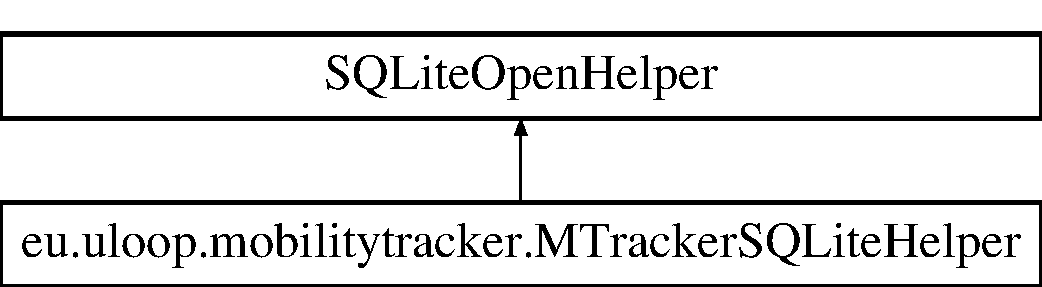
\includegraphics[height=2.000000cm]{classeu_1_1uloop_1_1mobilitytracker_1_1MTrackerSQLiteHelper}
\end{center}
\end{figure}
\subsection*{Public Member Functions}
\begin{DoxyCompactItemize}
\item 
\hyperlink{classeu_1_1uloop_1_1mobilitytracker_1_1MTrackerSQLiteHelper_a1ca4249f4dfa52e61e08778b12b5c056}{M\+Tracker\+S\+Q\+Lite\+Helper} (Context context)
\item 
void \hyperlink{classeu_1_1uloop_1_1mobilitytracker_1_1MTrackerSQLiteHelper_ac080af460b5d652bf95d1ef50f97cde1}{on\+Create} (S\+Q\+Lite\+Database data\+Base)
\item 
void \hyperlink{classeu_1_1uloop_1_1mobilitytracker_1_1MTrackerSQLiteHelper_a4fa12861aa7595d6dd4a80d3f192adad}{on\+Upgrade} (S\+Q\+Lite\+Database data\+Base, int old\+Version, int new\+Version)
\end{DoxyCompactItemize}
\subsection*{Static Public Attributes}
\begin{DoxyCompactItemize}
\item 
static final String \hyperlink{classeu_1_1uloop_1_1mobilitytracker_1_1MTrackerSQLiteHelper_aa89b29bbc519ff0ae0ce75eedc22eed0}{T\+A\+B\+L\+E\+\_\+\+A\+C\+C\+E\+S\+S\+P\+O\+I\+N\+T\+S} = \char`\"{}accesspoints\char`\"{}
\item 
static final String \hyperlink{classeu_1_1uloop_1_1mobilitytracker_1_1MTrackerSQLiteHelper_ab293b3268a1eb8edf543718500f3e39b}{T\+A\+B\+L\+E\+\_\+\+V\+I\+S\+I\+T\+S} = \char`\"{}visits\char`\"{}
\item 
static final String \hyperlink{classeu_1_1uloop_1_1mobilitytracker_1_1MTrackerSQLiteHelper_a4fdfca87f269093d65f48fae8cc762ed}{T\+A\+B\+L\+E\+\_\+\+C\+O\+N\+T\+E\+X\+T} = \char`\"{}context\char`\"{}
\item 
static final String \hyperlink{classeu_1_1uloop_1_1mobilitytracker_1_1MTrackerSQLiteHelper_a936bbd64784241550843b756745f60b4}{C\+O\+L\+U\+M\+N\+\_\+\+I\+D} = \char`\"{}\+\_\+id\char`\"{}
\item 
static final String \hyperlink{classeu_1_1uloop_1_1mobilitytracker_1_1MTrackerSQLiteHelper_af6bb71aa2cc6175bcb321e18a1e9661a}{C\+O\+L\+U\+M\+N\+\_\+\+S\+S\+I\+D} = \char`\"{}ssid\char`\"{}
\item 
static final String \hyperlink{classeu_1_1uloop_1_1mobilitytracker_1_1MTrackerSQLiteHelper_a482a1e79eb5a97433e61eb70ca7b6ae5}{C\+O\+L\+U\+M\+N\+\_\+\+B\+S\+S\+I\+D} = \char`\"{}bssid\char`\"{}
\item 
static final String \hyperlink{classeu_1_1uloop_1_1mobilitytracker_1_1MTrackerSQLiteHelper_a98c0cd9d0f3c95f884ebe211ab31275e}{C\+O\+L\+U\+M\+N\+\_\+\+G\+R\+O\+U\+P\+I\+D} = \char`\"{}groupid\char`\"{}
\item 
static final String \hyperlink{classeu_1_1uloop_1_1mobilitytracker_1_1MTrackerSQLiteHelper_a41b26bdadaacd6e05385c6190d4f3a58}{C\+O\+L\+U\+M\+N\+\_\+\+A\+T\+T\+R\+A\+C\+T\+I\+V\+E\+N\+E\+S\+S} = \char`\"{}attractiveness\char`\"{}
\item 
static final String \hyperlink{classeu_1_1uloop_1_1mobilitytracker_1_1MTrackerSQLiteHelper_a90da61fce9755e3b09097773cac0b693}{C\+O\+L\+U\+M\+N\+\_\+\+L\+A\+S\+T\+G\+A\+T\+E\+W\+A\+Y\+I\+P} = \char`\"{}lastgatewayip\char`\"{}
\item 
static final String \hyperlink{classeu_1_1uloop_1_1mobilitytracker_1_1MTrackerSQLiteHelper_aa2b425e08d18a595ea42c70fd9de4423}{C\+O\+L\+U\+M\+N\+\_\+\+T\+I\+M\+E\+O\+N} = \char`\"{}timeon\char`\"{}
\item 
static final String \hyperlink{classeu_1_1uloop_1_1mobilitytracker_1_1MTrackerSQLiteHelper_a761812af62579d365fde6a593cf31866}{C\+O\+L\+U\+M\+N\+\_\+\+T\+I\+M\+E\+O\+U\+T} = \char`\"{}timeout\char`\"{}
\item 
static final String \hyperlink{classeu_1_1uloop_1_1mobilitytracker_1_1MTrackerSQLiteHelper_a3a9dfdbca4fb3d30b30172c0a487a7c5}{C\+O\+L\+U\+M\+N\+\_\+\+D\+A\+Y\+O\+F\+T\+H\+E\+W\+E\+E\+K} = \char`\"{}dayoftheweek\char`\"{}
\item 
static final String \hyperlink{classeu_1_1uloop_1_1mobilitytracker_1_1MTrackerSQLiteHelper_ab751362436de50053ae1ca3658d9daf7}{C\+O\+L\+U\+M\+N\+\_\+\+H\+O\+U\+R} = \char`\"{}hour\char`\"{}
\end{DoxyCompactItemize}
\subsection*{Static Private Attributes}
\begin{DoxyCompactItemize}
\item 
static final String \hyperlink{classeu_1_1uloop_1_1mobilitytracker_1_1MTrackerSQLiteHelper_a1f7f36d98e2029a6762570819316845b}{D\+A\+T\+A\+B\+A\+S\+E\+\_\+\+N\+A\+M\+E} = \char`\"{}mtracker.\+db\char`\"{}
\item 
static final int \hyperlink{classeu_1_1uloop_1_1mobilitytracker_1_1MTrackerSQLiteHelper_a7b466275dbb75ef6c54d3f042da1e571}{D\+A\+T\+A\+B\+A\+S\+E\+\_\+\+V\+E\+R\+S\+I\+O\+N} = 1
\item 
static final String \hyperlink{classeu_1_1uloop_1_1mobilitytracker_1_1MTrackerSQLiteHelper_aa30b15bfbdcf226965b5ef3bf9a4a164}{C\+R\+E\+A\+T\+E\+\_\+\+A\+C\+C\+E\+S\+S\+P\+O\+I\+N\+T\+S\+\_\+\+T\+A\+B\+L\+E}
\item 
static final String \hyperlink{classeu_1_1uloop_1_1mobilitytracker_1_1MTrackerSQLiteHelper_a6c7b3e25a18753bd6115f606d7d9c1fc}{C\+R\+E\+A\+T\+E\+\_\+\+V\+I\+S\+I\+T\+S\+\_\+\+T\+A\+B\+L\+E}
\end{DoxyCompactItemize}


\subsection{Detailed Description}
This class extends the S\+Q\+Lite\+Open\+Helper android class.

\begin{DoxyAuthor}{Author}
Jonnahtan Saltarin (U\+L\+H\+T) 

Rute Sofia (U\+L\+H\+T) 

Christian da Silva Pereira (U\+L\+H\+T) 

Luis Amaral Lopes (U\+L\+H\+T)
\end{DoxyAuthor}
\begin{DoxyVersion}{Version}
3.\+0 
\end{DoxyVersion}


\subsection{Constructor \& Destructor Documentation}
\hypertarget{classeu_1_1uloop_1_1mobilitytracker_1_1MTrackerSQLiteHelper_a1ca4249f4dfa52e61e08778b12b5c056}{\index{eu\+::uloop\+::mobilitytracker\+::\+M\+Tracker\+S\+Q\+Lite\+Helper@{eu\+::uloop\+::mobilitytracker\+::\+M\+Tracker\+S\+Q\+Lite\+Helper}!M\+Tracker\+S\+Q\+Lite\+Helper@{M\+Tracker\+S\+Q\+Lite\+Helper}}
\index{M\+Tracker\+S\+Q\+Lite\+Helper@{M\+Tracker\+S\+Q\+Lite\+Helper}!eu\+::uloop\+::mobilitytracker\+::\+M\+Tracker\+S\+Q\+Lite\+Helper@{eu\+::uloop\+::mobilitytracker\+::\+M\+Tracker\+S\+Q\+Lite\+Helper}}
\subsubsection[{M\+Tracker\+S\+Q\+Lite\+Helper}]{\setlength{\rightskip}{0pt plus 5cm}eu.\+uloop.\+mobilitytracker.\+M\+Tracker\+S\+Q\+Lite\+Helper.\+M\+Tracker\+S\+Q\+Lite\+Helper (
\begin{DoxyParamCaption}
\item[{Context}]{context}
\end{DoxyParamCaption}
)}}\label{classeu_1_1uloop_1_1mobilitytracker_1_1MTrackerSQLiteHelper_a1ca4249f4dfa52e61e08778b12b5c056}


\subsection{Member Function Documentation}
\hypertarget{classeu_1_1uloop_1_1mobilitytracker_1_1MTrackerSQLiteHelper_ac080af460b5d652bf95d1ef50f97cde1}{\index{eu\+::uloop\+::mobilitytracker\+::\+M\+Tracker\+S\+Q\+Lite\+Helper@{eu\+::uloop\+::mobilitytracker\+::\+M\+Tracker\+S\+Q\+Lite\+Helper}!on\+Create@{on\+Create}}
\index{on\+Create@{on\+Create}!eu\+::uloop\+::mobilitytracker\+::\+M\+Tracker\+S\+Q\+Lite\+Helper@{eu\+::uloop\+::mobilitytracker\+::\+M\+Tracker\+S\+Q\+Lite\+Helper}}
\subsubsection[{on\+Create}]{\setlength{\rightskip}{0pt plus 5cm}void eu.\+uloop.\+mobilitytracker.\+M\+Tracker\+S\+Q\+Lite\+Helper.\+on\+Create (
\begin{DoxyParamCaption}
\item[{S\+Q\+Lite\+Database}]{data\+Base}
\end{DoxyParamCaption}
)}}\label{classeu_1_1uloop_1_1mobilitytracker_1_1MTrackerSQLiteHelper_ac080af460b5d652bf95d1ef50f97cde1}
\hypertarget{classeu_1_1uloop_1_1mobilitytracker_1_1MTrackerSQLiteHelper_a4fa12861aa7595d6dd4a80d3f192adad}{\index{eu\+::uloop\+::mobilitytracker\+::\+M\+Tracker\+S\+Q\+Lite\+Helper@{eu\+::uloop\+::mobilitytracker\+::\+M\+Tracker\+S\+Q\+Lite\+Helper}!on\+Upgrade@{on\+Upgrade}}
\index{on\+Upgrade@{on\+Upgrade}!eu\+::uloop\+::mobilitytracker\+::\+M\+Tracker\+S\+Q\+Lite\+Helper@{eu\+::uloop\+::mobilitytracker\+::\+M\+Tracker\+S\+Q\+Lite\+Helper}}
\subsubsection[{on\+Upgrade}]{\setlength{\rightskip}{0pt plus 5cm}void eu.\+uloop.\+mobilitytracker.\+M\+Tracker\+S\+Q\+Lite\+Helper.\+on\+Upgrade (
\begin{DoxyParamCaption}
\item[{S\+Q\+Lite\+Database}]{data\+Base, }
\item[{int}]{old\+Version, }
\item[{int}]{new\+Version}
\end{DoxyParamCaption}
)}}\label{classeu_1_1uloop_1_1mobilitytracker_1_1MTrackerSQLiteHelper_a4fa12861aa7595d6dd4a80d3f192adad}


\subsection{Member Data Documentation}
\hypertarget{classeu_1_1uloop_1_1mobilitytracker_1_1MTrackerSQLiteHelper_a41b26bdadaacd6e05385c6190d4f3a58}{\index{eu\+::uloop\+::mobilitytracker\+::\+M\+Tracker\+S\+Q\+Lite\+Helper@{eu\+::uloop\+::mobilitytracker\+::\+M\+Tracker\+S\+Q\+Lite\+Helper}!C\+O\+L\+U\+M\+N\+\_\+\+A\+T\+T\+R\+A\+C\+T\+I\+V\+E\+N\+E\+S\+S@{C\+O\+L\+U\+M\+N\+\_\+\+A\+T\+T\+R\+A\+C\+T\+I\+V\+E\+N\+E\+S\+S}}
\index{C\+O\+L\+U\+M\+N\+\_\+\+A\+T\+T\+R\+A\+C\+T\+I\+V\+E\+N\+E\+S\+S@{C\+O\+L\+U\+M\+N\+\_\+\+A\+T\+T\+R\+A\+C\+T\+I\+V\+E\+N\+E\+S\+S}!eu\+::uloop\+::mobilitytracker\+::\+M\+Tracker\+S\+Q\+Lite\+Helper@{eu\+::uloop\+::mobilitytracker\+::\+M\+Tracker\+S\+Q\+Lite\+Helper}}
\subsubsection[{C\+O\+L\+U\+M\+N\+\_\+\+A\+T\+T\+R\+A\+C\+T\+I\+V\+E\+N\+E\+S\+S}]{\setlength{\rightskip}{0pt plus 5cm}final String eu.\+uloop.\+mobilitytracker.\+M\+Tracker\+S\+Q\+Lite\+Helper.\+C\+O\+L\+U\+M\+N\+\_\+\+A\+T\+T\+R\+A\+C\+T\+I\+V\+E\+N\+E\+S\+S = \char`\"{}attractiveness\char`\"{}\hspace{0.3cm}{\ttfamily [static]}}}\label{classeu_1_1uloop_1_1mobilitytracker_1_1MTrackerSQLiteHelper_a41b26bdadaacd6e05385c6190d4f3a58}
\hypertarget{classeu_1_1uloop_1_1mobilitytracker_1_1MTrackerSQLiteHelper_a482a1e79eb5a97433e61eb70ca7b6ae5}{\index{eu\+::uloop\+::mobilitytracker\+::\+M\+Tracker\+S\+Q\+Lite\+Helper@{eu\+::uloop\+::mobilitytracker\+::\+M\+Tracker\+S\+Q\+Lite\+Helper}!C\+O\+L\+U\+M\+N\+\_\+\+B\+S\+S\+I\+D@{C\+O\+L\+U\+M\+N\+\_\+\+B\+S\+S\+I\+D}}
\index{C\+O\+L\+U\+M\+N\+\_\+\+B\+S\+S\+I\+D@{C\+O\+L\+U\+M\+N\+\_\+\+B\+S\+S\+I\+D}!eu\+::uloop\+::mobilitytracker\+::\+M\+Tracker\+S\+Q\+Lite\+Helper@{eu\+::uloop\+::mobilitytracker\+::\+M\+Tracker\+S\+Q\+Lite\+Helper}}
\subsubsection[{C\+O\+L\+U\+M\+N\+\_\+\+B\+S\+S\+I\+D}]{\setlength{\rightskip}{0pt plus 5cm}final String eu.\+uloop.\+mobilitytracker.\+M\+Tracker\+S\+Q\+Lite\+Helper.\+C\+O\+L\+U\+M\+N\+\_\+\+B\+S\+S\+I\+D = \char`\"{}bssid\char`\"{}\hspace{0.3cm}{\ttfamily [static]}}}\label{classeu_1_1uloop_1_1mobilitytracker_1_1MTrackerSQLiteHelper_a482a1e79eb5a97433e61eb70ca7b6ae5}
\hypertarget{classeu_1_1uloop_1_1mobilitytracker_1_1MTrackerSQLiteHelper_a3a9dfdbca4fb3d30b30172c0a487a7c5}{\index{eu\+::uloop\+::mobilitytracker\+::\+M\+Tracker\+S\+Q\+Lite\+Helper@{eu\+::uloop\+::mobilitytracker\+::\+M\+Tracker\+S\+Q\+Lite\+Helper}!C\+O\+L\+U\+M\+N\+\_\+\+D\+A\+Y\+O\+F\+T\+H\+E\+W\+E\+E\+K@{C\+O\+L\+U\+M\+N\+\_\+\+D\+A\+Y\+O\+F\+T\+H\+E\+W\+E\+E\+K}}
\index{C\+O\+L\+U\+M\+N\+\_\+\+D\+A\+Y\+O\+F\+T\+H\+E\+W\+E\+E\+K@{C\+O\+L\+U\+M\+N\+\_\+\+D\+A\+Y\+O\+F\+T\+H\+E\+W\+E\+E\+K}!eu\+::uloop\+::mobilitytracker\+::\+M\+Tracker\+S\+Q\+Lite\+Helper@{eu\+::uloop\+::mobilitytracker\+::\+M\+Tracker\+S\+Q\+Lite\+Helper}}
\subsubsection[{C\+O\+L\+U\+M\+N\+\_\+\+D\+A\+Y\+O\+F\+T\+H\+E\+W\+E\+E\+K}]{\setlength{\rightskip}{0pt plus 5cm}final String eu.\+uloop.\+mobilitytracker.\+M\+Tracker\+S\+Q\+Lite\+Helper.\+C\+O\+L\+U\+M\+N\+\_\+\+D\+A\+Y\+O\+F\+T\+H\+E\+W\+E\+E\+K = \char`\"{}dayoftheweek\char`\"{}\hspace{0.3cm}{\ttfamily [static]}}}\label{classeu_1_1uloop_1_1mobilitytracker_1_1MTrackerSQLiteHelper_a3a9dfdbca4fb3d30b30172c0a487a7c5}
\hypertarget{classeu_1_1uloop_1_1mobilitytracker_1_1MTrackerSQLiteHelper_a98c0cd9d0f3c95f884ebe211ab31275e}{\index{eu\+::uloop\+::mobilitytracker\+::\+M\+Tracker\+S\+Q\+Lite\+Helper@{eu\+::uloop\+::mobilitytracker\+::\+M\+Tracker\+S\+Q\+Lite\+Helper}!C\+O\+L\+U\+M\+N\+\_\+\+G\+R\+O\+U\+P\+I\+D@{C\+O\+L\+U\+M\+N\+\_\+\+G\+R\+O\+U\+P\+I\+D}}
\index{C\+O\+L\+U\+M\+N\+\_\+\+G\+R\+O\+U\+P\+I\+D@{C\+O\+L\+U\+M\+N\+\_\+\+G\+R\+O\+U\+P\+I\+D}!eu\+::uloop\+::mobilitytracker\+::\+M\+Tracker\+S\+Q\+Lite\+Helper@{eu\+::uloop\+::mobilitytracker\+::\+M\+Tracker\+S\+Q\+Lite\+Helper}}
\subsubsection[{C\+O\+L\+U\+M\+N\+\_\+\+G\+R\+O\+U\+P\+I\+D}]{\setlength{\rightskip}{0pt plus 5cm}final String eu.\+uloop.\+mobilitytracker.\+M\+Tracker\+S\+Q\+Lite\+Helper.\+C\+O\+L\+U\+M\+N\+\_\+\+G\+R\+O\+U\+P\+I\+D = \char`\"{}groupid\char`\"{}\hspace{0.3cm}{\ttfamily [static]}}}\label{classeu_1_1uloop_1_1mobilitytracker_1_1MTrackerSQLiteHelper_a98c0cd9d0f3c95f884ebe211ab31275e}
\hypertarget{classeu_1_1uloop_1_1mobilitytracker_1_1MTrackerSQLiteHelper_ab751362436de50053ae1ca3658d9daf7}{\index{eu\+::uloop\+::mobilitytracker\+::\+M\+Tracker\+S\+Q\+Lite\+Helper@{eu\+::uloop\+::mobilitytracker\+::\+M\+Tracker\+S\+Q\+Lite\+Helper}!C\+O\+L\+U\+M\+N\+\_\+\+H\+O\+U\+R@{C\+O\+L\+U\+M\+N\+\_\+\+H\+O\+U\+R}}
\index{C\+O\+L\+U\+M\+N\+\_\+\+H\+O\+U\+R@{C\+O\+L\+U\+M\+N\+\_\+\+H\+O\+U\+R}!eu\+::uloop\+::mobilitytracker\+::\+M\+Tracker\+S\+Q\+Lite\+Helper@{eu\+::uloop\+::mobilitytracker\+::\+M\+Tracker\+S\+Q\+Lite\+Helper}}
\subsubsection[{C\+O\+L\+U\+M\+N\+\_\+\+H\+O\+U\+R}]{\setlength{\rightskip}{0pt plus 5cm}final String eu.\+uloop.\+mobilitytracker.\+M\+Tracker\+S\+Q\+Lite\+Helper.\+C\+O\+L\+U\+M\+N\+\_\+\+H\+O\+U\+R = \char`\"{}hour\char`\"{}\hspace{0.3cm}{\ttfamily [static]}}}\label{classeu_1_1uloop_1_1mobilitytracker_1_1MTrackerSQLiteHelper_ab751362436de50053ae1ca3658d9daf7}
\hypertarget{classeu_1_1uloop_1_1mobilitytracker_1_1MTrackerSQLiteHelper_a936bbd64784241550843b756745f60b4}{\index{eu\+::uloop\+::mobilitytracker\+::\+M\+Tracker\+S\+Q\+Lite\+Helper@{eu\+::uloop\+::mobilitytracker\+::\+M\+Tracker\+S\+Q\+Lite\+Helper}!C\+O\+L\+U\+M\+N\+\_\+\+I\+D@{C\+O\+L\+U\+M\+N\+\_\+\+I\+D}}
\index{C\+O\+L\+U\+M\+N\+\_\+\+I\+D@{C\+O\+L\+U\+M\+N\+\_\+\+I\+D}!eu\+::uloop\+::mobilitytracker\+::\+M\+Tracker\+S\+Q\+Lite\+Helper@{eu\+::uloop\+::mobilitytracker\+::\+M\+Tracker\+S\+Q\+Lite\+Helper}}
\subsubsection[{C\+O\+L\+U\+M\+N\+\_\+\+I\+D}]{\setlength{\rightskip}{0pt plus 5cm}final String eu.\+uloop.\+mobilitytracker.\+M\+Tracker\+S\+Q\+Lite\+Helper.\+C\+O\+L\+U\+M\+N\+\_\+\+I\+D = \char`\"{}\+\_\+id\char`\"{}\hspace{0.3cm}{\ttfamily [static]}}}\label{classeu_1_1uloop_1_1mobilitytracker_1_1MTrackerSQLiteHelper_a936bbd64784241550843b756745f60b4}
\hypertarget{classeu_1_1uloop_1_1mobilitytracker_1_1MTrackerSQLiteHelper_a90da61fce9755e3b09097773cac0b693}{\index{eu\+::uloop\+::mobilitytracker\+::\+M\+Tracker\+S\+Q\+Lite\+Helper@{eu\+::uloop\+::mobilitytracker\+::\+M\+Tracker\+S\+Q\+Lite\+Helper}!C\+O\+L\+U\+M\+N\+\_\+\+L\+A\+S\+T\+G\+A\+T\+E\+W\+A\+Y\+I\+P@{C\+O\+L\+U\+M\+N\+\_\+\+L\+A\+S\+T\+G\+A\+T\+E\+W\+A\+Y\+I\+P}}
\index{C\+O\+L\+U\+M\+N\+\_\+\+L\+A\+S\+T\+G\+A\+T\+E\+W\+A\+Y\+I\+P@{C\+O\+L\+U\+M\+N\+\_\+\+L\+A\+S\+T\+G\+A\+T\+E\+W\+A\+Y\+I\+P}!eu\+::uloop\+::mobilitytracker\+::\+M\+Tracker\+S\+Q\+Lite\+Helper@{eu\+::uloop\+::mobilitytracker\+::\+M\+Tracker\+S\+Q\+Lite\+Helper}}
\subsubsection[{C\+O\+L\+U\+M\+N\+\_\+\+L\+A\+S\+T\+G\+A\+T\+E\+W\+A\+Y\+I\+P}]{\setlength{\rightskip}{0pt plus 5cm}final String eu.\+uloop.\+mobilitytracker.\+M\+Tracker\+S\+Q\+Lite\+Helper.\+C\+O\+L\+U\+M\+N\+\_\+\+L\+A\+S\+T\+G\+A\+T\+E\+W\+A\+Y\+I\+P = \char`\"{}lastgatewayip\char`\"{}\hspace{0.3cm}{\ttfamily [static]}}}\label{classeu_1_1uloop_1_1mobilitytracker_1_1MTrackerSQLiteHelper_a90da61fce9755e3b09097773cac0b693}
\hypertarget{classeu_1_1uloop_1_1mobilitytracker_1_1MTrackerSQLiteHelper_af6bb71aa2cc6175bcb321e18a1e9661a}{\index{eu\+::uloop\+::mobilitytracker\+::\+M\+Tracker\+S\+Q\+Lite\+Helper@{eu\+::uloop\+::mobilitytracker\+::\+M\+Tracker\+S\+Q\+Lite\+Helper}!C\+O\+L\+U\+M\+N\+\_\+\+S\+S\+I\+D@{C\+O\+L\+U\+M\+N\+\_\+\+S\+S\+I\+D}}
\index{C\+O\+L\+U\+M\+N\+\_\+\+S\+S\+I\+D@{C\+O\+L\+U\+M\+N\+\_\+\+S\+S\+I\+D}!eu\+::uloop\+::mobilitytracker\+::\+M\+Tracker\+S\+Q\+Lite\+Helper@{eu\+::uloop\+::mobilitytracker\+::\+M\+Tracker\+S\+Q\+Lite\+Helper}}
\subsubsection[{C\+O\+L\+U\+M\+N\+\_\+\+S\+S\+I\+D}]{\setlength{\rightskip}{0pt plus 5cm}final String eu.\+uloop.\+mobilitytracker.\+M\+Tracker\+S\+Q\+Lite\+Helper.\+C\+O\+L\+U\+M\+N\+\_\+\+S\+S\+I\+D = \char`\"{}ssid\char`\"{}\hspace{0.3cm}{\ttfamily [static]}}}\label{classeu_1_1uloop_1_1mobilitytracker_1_1MTrackerSQLiteHelper_af6bb71aa2cc6175bcb321e18a1e9661a}
\hypertarget{classeu_1_1uloop_1_1mobilitytracker_1_1MTrackerSQLiteHelper_aa2b425e08d18a595ea42c70fd9de4423}{\index{eu\+::uloop\+::mobilitytracker\+::\+M\+Tracker\+S\+Q\+Lite\+Helper@{eu\+::uloop\+::mobilitytracker\+::\+M\+Tracker\+S\+Q\+Lite\+Helper}!C\+O\+L\+U\+M\+N\+\_\+\+T\+I\+M\+E\+O\+N@{C\+O\+L\+U\+M\+N\+\_\+\+T\+I\+M\+E\+O\+N}}
\index{C\+O\+L\+U\+M\+N\+\_\+\+T\+I\+M\+E\+O\+N@{C\+O\+L\+U\+M\+N\+\_\+\+T\+I\+M\+E\+O\+N}!eu\+::uloop\+::mobilitytracker\+::\+M\+Tracker\+S\+Q\+Lite\+Helper@{eu\+::uloop\+::mobilitytracker\+::\+M\+Tracker\+S\+Q\+Lite\+Helper}}
\subsubsection[{C\+O\+L\+U\+M\+N\+\_\+\+T\+I\+M\+E\+O\+N}]{\setlength{\rightskip}{0pt plus 5cm}final String eu.\+uloop.\+mobilitytracker.\+M\+Tracker\+S\+Q\+Lite\+Helper.\+C\+O\+L\+U\+M\+N\+\_\+\+T\+I\+M\+E\+O\+N = \char`\"{}timeon\char`\"{}\hspace{0.3cm}{\ttfamily [static]}}}\label{classeu_1_1uloop_1_1mobilitytracker_1_1MTrackerSQLiteHelper_aa2b425e08d18a595ea42c70fd9de4423}
\hypertarget{classeu_1_1uloop_1_1mobilitytracker_1_1MTrackerSQLiteHelper_a761812af62579d365fde6a593cf31866}{\index{eu\+::uloop\+::mobilitytracker\+::\+M\+Tracker\+S\+Q\+Lite\+Helper@{eu\+::uloop\+::mobilitytracker\+::\+M\+Tracker\+S\+Q\+Lite\+Helper}!C\+O\+L\+U\+M\+N\+\_\+\+T\+I\+M\+E\+O\+U\+T@{C\+O\+L\+U\+M\+N\+\_\+\+T\+I\+M\+E\+O\+U\+T}}
\index{C\+O\+L\+U\+M\+N\+\_\+\+T\+I\+M\+E\+O\+U\+T@{C\+O\+L\+U\+M\+N\+\_\+\+T\+I\+M\+E\+O\+U\+T}!eu\+::uloop\+::mobilitytracker\+::\+M\+Tracker\+S\+Q\+Lite\+Helper@{eu\+::uloop\+::mobilitytracker\+::\+M\+Tracker\+S\+Q\+Lite\+Helper}}
\subsubsection[{C\+O\+L\+U\+M\+N\+\_\+\+T\+I\+M\+E\+O\+U\+T}]{\setlength{\rightskip}{0pt plus 5cm}final String eu.\+uloop.\+mobilitytracker.\+M\+Tracker\+S\+Q\+Lite\+Helper.\+C\+O\+L\+U\+M\+N\+\_\+\+T\+I\+M\+E\+O\+U\+T = \char`\"{}timeout\char`\"{}\hspace{0.3cm}{\ttfamily [static]}}}\label{classeu_1_1uloop_1_1mobilitytracker_1_1MTrackerSQLiteHelper_a761812af62579d365fde6a593cf31866}
\hypertarget{classeu_1_1uloop_1_1mobilitytracker_1_1MTrackerSQLiteHelper_aa30b15bfbdcf226965b5ef3bf9a4a164}{\index{eu\+::uloop\+::mobilitytracker\+::\+M\+Tracker\+S\+Q\+Lite\+Helper@{eu\+::uloop\+::mobilitytracker\+::\+M\+Tracker\+S\+Q\+Lite\+Helper}!C\+R\+E\+A\+T\+E\+\_\+\+A\+C\+C\+E\+S\+S\+P\+O\+I\+N\+T\+S\+\_\+\+T\+A\+B\+L\+E@{C\+R\+E\+A\+T\+E\+\_\+\+A\+C\+C\+E\+S\+S\+P\+O\+I\+N\+T\+S\+\_\+\+T\+A\+B\+L\+E}}
\index{C\+R\+E\+A\+T\+E\+\_\+\+A\+C\+C\+E\+S\+S\+P\+O\+I\+N\+T\+S\+\_\+\+T\+A\+B\+L\+E@{C\+R\+E\+A\+T\+E\+\_\+\+A\+C\+C\+E\+S\+S\+P\+O\+I\+N\+T\+S\+\_\+\+T\+A\+B\+L\+E}!eu\+::uloop\+::mobilitytracker\+::\+M\+Tracker\+S\+Q\+Lite\+Helper@{eu\+::uloop\+::mobilitytracker\+::\+M\+Tracker\+S\+Q\+Lite\+Helper}}
\subsubsection[{C\+R\+E\+A\+T\+E\+\_\+\+A\+C\+C\+E\+S\+S\+P\+O\+I\+N\+T\+S\+\_\+\+T\+A\+B\+L\+E}]{\setlength{\rightskip}{0pt plus 5cm}final String eu.\+uloop.\+mobilitytracker.\+M\+Tracker\+S\+Q\+Lite\+Helper.\+C\+R\+E\+A\+T\+E\+\_\+\+A\+C\+C\+E\+S\+S\+P\+O\+I\+N\+T\+S\+\_\+\+T\+A\+B\+L\+E\hspace{0.3cm}{\ttfamily [static]}, {\ttfamily [private]}}}\label{classeu_1_1uloop_1_1mobilitytracker_1_1MTrackerSQLiteHelper_aa30b15bfbdcf226965b5ef3bf9a4a164}
{\bfseries Initial value\+:}
\begin{DoxyCode}
= \textcolor{stringliteral}{"create table "}
                      + \hyperlink{classeu_1_1uloop_1_1mobilitytracker_1_1MTrackerSQLiteHelper_aa89b29bbc519ff0ae0ce75eedc22eed0}{TABLE\_ACCESSPOINTS} + \textcolor{stringliteral}{"("}
                      + \hyperlink{classeu_1_1uloop_1_1mobilitytracker_1_1MTrackerSQLiteHelper_a936bbd64784241550843b756745f60b4}{COLUMN\_ID} + \textcolor{stringliteral}{" integer primary key autoincrement, "}
                      + \hyperlink{classeu_1_1uloop_1_1mobilitytracker_1_1MTrackerSQLiteHelper_a482a1e79eb5a97433e61eb70ca7b6ae5}{COLUMN\_BSSID} + \textcolor{stringliteral}{" text not null unique, "}
                      + \hyperlink{classeu_1_1uloop_1_1mobilitytracker_1_1MTrackerSQLiteHelper_af6bb71aa2cc6175bcb321e18a1e9661a}{COLUMN\_SSID} + \textcolor{stringliteral}{" text not null unique, "}
                      + \hyperlink{classeu_1_1uloop_1_1mobilitytracker_1_1MTrackerSQLiteHelper_a41b26bdadaacd6e05385c6190d4f3a58}{COLUMN\_ATTRACTIVENESS} + \textcolor{stringliteral}{" integer not null, "}
                      + \hyperlink{classeu_1_1uloop_1_1mobilitytracker_1_1MTrackerSQLiteHelper_a90da61fce9755e3b09097773cac0b693}{COLUMN\_LASTGATEWAYIP} + \textcolor{stringliteral}{" text"}
                      + \textcolor{stringliteral}{");"}
\end{DoxyCode}
\hypertarget{classeu_1_1uloop_1_1mobilitytracker_1_1MTrackerSQLiteHelper_a6c7b3e25a18753bd6115f606d7d9c1fc}{\index{eu\+::uloop\+::mobilitytracker\+::\+M\+Tracker\+S\+Q\+Lite\+Helper@{eu\+::uloop\+::mobilitytracker\+::\+M\+Tracker\+S\+Q\+Lite\+Helper}!C\+R\+E\+A\+T\+E\+\_\+\+V\+I\+S\+I\+T\+S\+\_\+\+T\+A\+B\+L\+E@{C\+R\+E\+A\+T\+E\+\_\+\+V\+I\+S\+I\+T\+S\+\_\+\+T\+A\+B\+L\+E}}
\index{C\+R\+E\+A\+T\+E\+\_\+\+V\+I\+S\+I\+T\+S\+\_\+\+T\+A\+B\+L\+E@{C\+R\+E\+A\+T\+E\+\_\+\+V\+I\+S\+I\+T\+S\+\_\+\+T\+A\+B\+L\+E}!eu\+::uloop\+::mobilitytracker\+::\+M\+Tracker\+S\+Q\+Lite\+Helper@{eu\+::uloop\+::mobilitytracker\+::\+M\+Tracker\+S\+Q\+Lite\+Helper}}
\subsubsection[{C\+R\+E\+A\+T\+E\+\_\+\+V\+I\+S\+I\+T\+S\+\_\+\+T\+A\+B\+L\+E}]{\setlength{\rightskip}{0pt plus 5cm}final String eu.\+uloop.\+mobilitytracker.\+M\+Tracker\+S\+Q\+Lite\+Helper.\+C\+R\+E\+A\+T\+E\+\_\+\+V\+I\+S\+I\+T\+S\+\_\+\+T\+A\+B\+L\+E\hspace{0.3cm}{\ttfamily [static]}, {\ttfamily [private]}}}\label{classeu_1_1uloop_1_1mobilitytracker_1_1MTrackerSQLiteHelper_a6c7b3e25a18753bd6115f606d7d9c1fc}
{\bfseries Initial value\+:}
\begin{DoxyCode}
= \textcolor{stringliteral}{"create table "}
                      + \hyperlink{classeu_1_1uloop_1_1mobilitytracker_1_1MTrackerSQLiteHelper_ab293b3268a1eb8edf543718500f3e39b}{TABLE\_VISITS} + \textcolor{stringliteral}{"("}
                      + \hyperlink{classeu_1_1uloop_1_1mobilitytracker_1_1MTrackerSQLiteHelper_a936bbd64784241550843b756745f60b4}{COLUMN\_ID} + \textcolor{stringliteral}{" integer primary key autoincrement, "}
                      + \hyperlink{classeu_1_1uloop_1_1mobilitytracker_1_1MTrackerSQLiteHelper_af6bb71aa2cc6175bcb321e18a1e9661a}{COLUMN\_SSID} + \textcolor{stringliteral}{" text not null, "}
                      + \hyperlink{classeu_1_1uloop_1_1mobilitytracker_1_1MTrackerSQLiteHelper_a482a1e79eb5a97433e61eb70ca7b6ae5}{COLUMN\_BSSID} + \textcolor{stringliteral}{" text not null, "}
                      + \hyperlink{classeu_1_1uloop_1_1mobilitytracker_1_1MTrackerSQLiteHelper_aa2b425e08d18a595ea42c70fd9de4423}{COLUMN\_TIMEON} + \textcolor{stringliteral}{" integer, "}
                      + \hyperlink{classeu_1_1uloop_1_1mobilitytracker_1_1MTrackerSQLiteHelper_a761812af62579d365fde6a593cf31866}{COLUMN\_TIMEOUT} + \textcolor{stringliteral}{" integer, "}
                      + \hyperlink{classeu_1_1uloop_1_1mobilitytracker_1_1MTrackerSQLiteHelper_a3a9dfdbca4fb3d30b30172c0a487a7c5}{COLUMN\_DAYOFTHEWEEK} + \textcolor{stringliteral}{" integer, "}
                      + \hyperlink{classeu_1_1uloop_1_1mobilitytracker_1_1MTrackerSQLiteHelper_ab751362436de50053ae1ca3658d9daf7}{COLUMN\_HOUR} + \textcolor{stringliteral}{" integer"}
                      + \textcolor{stringliteral}{");"}
\end{DoxyCode}
\hypertarget{classeu_1_1uloop_1_1mobilitytracker_1_1MTrackerSQLiteHelper_a1f7f36d98e2029a6762570819316845b}{\index{eu\+::uloop\+::mobilitytracker\+::\+M\+Tracker\+S\+Q\+Lite\+Helper@{eu\+::uloop\+::mobilitytracker\+::\+M\+Tracker\+S\+Q\+Lite\+Helper}!D\+A\+T\+A\+B\+A\+S\+E\+\_\+\+N\+A\+M\+E@{D\+A\+T\+A\+B\+A\+S\+E\+\_\+\+N\+A\+M\+E}}
\index{D\+A\+T\+A\+B\+A\+S\+E\+\_\+\+N\+A\+M\+E@{D\+A\+T\+A\+B\+A\+S\+E\+\_\+\+N\+A\+M\+E}!eu\+::uloop\+::mobilitytracker\+::\+M\+Tracker\+S\+Q\+Lite\+Helper@{eu\+::uloop\+::mobilitytracker\+::\+M\+Tracker\+S\+Q\+Lite\+Helper}}
\subsubsection[{D\+A\+T\+A\+B\+A\+S\+E\+\_\+\+N\+A\+M\+E}]{\setlength{\rightskip}{0pt plus 5cm}final String eu.\+uloop.\+mobilitytracker.\+M\+Tracker\+S\+Q\+Lite\+Helper.\+D\+A\+T\+A\+B\+A\+S\+E\+\_\+\+N\+A\+M\+E = \char`\"{}mtracker.\+db\char`\"{}\hspace{0.3cm}{\ttfamily [static]}, {\ttfamily [private]}}}\label{classeu_1_1uloop_1_1mobilitytracker_1_1MTrackerSQLiteHelper_a1f7f36d98e2029a6762570819316845b}
\hypertarget{classeu_1_1uloop_1_1mobilitytracker_1_1MTrackerSQLiteHelper_a7b466275dbb75ef6c54d3f042da1e571}{\index{eu\+::uloop\+::mobilitytracker\+::\+M\+Tracker\+S\+Q\+Lite\+Helper@{eu\+::uloop\+::mobilitytracker\+::\+M\+Tracker\+S\+Q\+Lite\+Helper}!D\+A\+T\+A\+B\+A\+S\+E\+\_\+\+V\+E\+R\+S\+I\+O\+N@{D\+A\+T\+A\+B\+A\+S\+E\+\_\+\+V\+E\+R\+S\+I\+O\+N}}
\index{D\+A\+T\+A\+B\+A\+S\+E\+\_\+\+V\+E\+R\+S\+I\+O\+N@{D\+A\+T\+A\+B\+A\+S\+E\+\_\+\+V\+E\+R\+S\+I\+O\+N}!eu\+::uloop\+::mobilitytracker\+::\+M\+Tracker\+S\+Q\+Lite\+Helper@{eu\+::uloop\+::mobilitytracker\+::\+M\+Tracker\+S\+Q\+Lite\+Helper}}
\subsubsection[{D\+A\+T\+A\+B\+A\+S\+E\+\_\+\+V\+E\+R\+S\+I\+O\+N}]{\setlength{\rightskip}{0pt plus 5cm}final int eu.\+uloop.\+mobilitytracker.\+M\+Tracker\+S\+Q\+Lite\+Helper.\+D\+A\+T\+A\+B\+A\+S\+E\+\_\+\+V\+E\+R\+S\+I\+O\+N = 1\hspace{0.3cm}{\ttfamily [static]}, {\ttfamily [private]}}}\label{classeu_1_1uloop_1_1mobilitytracker_1_1MTrackerSQLiteHelper_a7b466275dbb75ef6c54d3f042da1e571}
\hypertarget{classeu_1_1uloop_1_1mobilitytracker_1_1MTrackerSQLiteHelper_aa89b29bbc519ff0ae0ce75eedc22eed0}{\index{eu\+::uloop\+::mobilitytracker\+::\+M\+Tracker\+S\+Q\+Lite\+Helper@{eu\+::uloop\+::mobilitytracker\+::\+M\+Tracker\+S\+Q\+Lite\+Helper}!T\+A\+B\+L\+E\+\_\+\+A\+C\+C\+E\+S\+S\+P\+O\+I\+N\+T\+S@{T\+A\+B\+L\+E\+\_\+\+A\+C\+C\+E\+S\+S\+P\+O\+I\+N\+T\+S}}
\index{T\+A\+B\+L\+E\+\_\+\+A\+C\+C\+E\+S\+S\+P\+O\+I\+N\+T\+S@{T\+A\+B\+L\+E\+\_\+\+A\+C\+C\+E\+S\+S\+P\+O\+I\+N\+T\+S}!eu\+::uloop\+::mobilitytracker\+::\+M\+Tracker\+S\+Q\+Lite\+Helper@{eu\+::uloop\+::mobilitytracker\+::\+M\+Tracker\+S\+Q\+Lite\+Helper}}
\subsubsection[{T\+A\+B\+L\+E\+\_\+\+A\+C\+C\+E\+S\+S\+P\+O\+I\+N\+T\+S}]{\setlength{\rightskip}{0pt plus 5cm}final String eu.\+uloop.\+mobilitytracker.\+M\+Tracker\+S\+Q\+Lite\+Helper.\+T\+A\+B\+L\+E\+\_\+\+A\+C\+C\+E\+S\+S\+P\+O\+I\+N\+T\+S = \char`\"{}accesspoints\char`\"{}\hspace{0.3cm}{\ttfamily [static]}}}\label{classeu_1_1uloop_1_1mobilitytracker_1_1MTrackerSQLiteHelper_aa89b29bbc519ff0ae0ce75eedc22eed0}
\hypertarget{classeu_1_1uloop_1_1mobilitytracker_1_1MTrackerSQLiteHelper_a4fdfca87f269093d65f48fae8cc762ed}{\index{eu\+::uloop\+::mobilitytracker\+::\+M\+Tracker\+S\+Q\+Lite\+Helper@{eu\+::uloop\+::mobilitytracker\+::\+M\+Tracker\+S\+Q\+Lite\+Helper}!T\+A\+B\+L\+E\+\_\+\+C\+O\+N\+T\+E\+X\+T@{T\+A\+B\+L\+E\+\_\+\+C\+O\+N\+T\+E\+X\+T}}
\index{T\+A\+B\+L\+E\+\_\+\+C\+O\+N\+T\+E\+X\+T@{T\+A\+B\+L\+E\+\_\+\+C\+O\+N\+T\+E\+X\+T}!eu\+::uloop\+::mobilitytracker\+::\+M\+Tracker\+S\+Q\+Lite\+Helper@{eu\+::uloop\+::mobilitytracker\+::\+M\+Tracker\+S\+Q\+Lite\+Helper}}
\subsubsection[{T\+A\+B\+L\+E\+\_\+\+C\+O\+N\+T\+E\+X\+T}]{\setlength{\rightskip}{0pt plus 5cm}final String eu.\+uloop.\+mobilitytracker.\+M\+Tracker\+S\+Q\+Lite\+Helper.\+T\+A\+B\+L\+E\+\_\+\+C\+O\+N\+T\+E\+X\+T = \char`\"{}context\char`\"{}\hspace{0.3cm}{\ttfamily [static]}}}\label{classeu_1_1uloop_1_1mobilitytracker_1_1MTrackerSQLiteHelper_a4fdfca87f269093d65f48fae8cc762ed}
\hypertarget{classeu_1_1uloop_1_1mobilitytracker_1_1MTrackerSQLiteHelper_ab293b3268a1eb8edf543718500f3e39b}{\index{eu\+::uloop\+::mobilitytracker\+::\+M\+Tracker\+S\+Q\+Lite\+Helper@{eu\+::uloop\+::mobilitytracker\+::\+M\+Tracker\+S\+Q\+Lite\+Helper}!T\+A\+B\+L\+E\+\_\+\+V\+I\+S\+I\+T\+S@{T\+A\+B\+L\+E\+\_\+\+V\+I\+S\+I\+T\+S}}
\index{T\+A\+B\+L\+E\+\_\+\+V\+I\+S\+I\+T\+S@{T\+A\+B\+L\+E\+\_\+\+V\+I\+S\+I\+T\+S}!eu\+::uloop\+::mobilitytracker\+::\+M\+Tracker\+S\+Q\+Lite\+Helper@{eu\+::uloop\+::mobilitytracker\+::\+M\+Tracker\+S\+Q\+Lite\+Helper}}
\subsubsection[{T\+A\+B\+L\+E\+\_\+\+V\+I\+S\+I\+T\+S}]{\setlength{\rightskip}{0pt plus 5cm}final String eu.\+uloop.\+mobilitytracker.\+M\+Tracker\+S\+Q\+Lite\+Helper.\+T\+A\+B\+L\+E\+\_\+\+V\+I\+S\+I\+T\+S = \char`\"{}visits\char`\"{}\hspace{0.3cm}{\ttfamily [static]}}}\label{classeu_1_1uloop_1_1mobilitytracker_1_1MTrackerSQLiteHelper_ab293b3268a1eb8edf543718500f3e39b}


The documentation for this class was generated from the following file\+:\begin{DoxyCompactItemize}
\item 
src/eu/uloop/mobilitytracker/\hyperlink{MTrackerSQLiteHelper_8java}{M\+Tracker\+S\+Q\+Lite\+Helper.\+java}\end{DoxyCompactItemize}

\hypertarget{classeu_1_1uloop_1_1mobilitytracker_1_1MTrackerVisit}{\section{eu.\+uloop.\+mobilitytracker.\+M\+Tracker\+Visit Class Reference}
\label{classeu_1_1uloop_1_1mobilitytracker_1_1MTrackerVisit}\index{eu.\+uloop.\+mobilitytracker.\+M\+Tracker\+Visit@{eu.\+uloop.\+mobilitytracker.\+M\+Tracker\+Visit}}
}
\subsection*{Public Member Functions}
\begin{DoxyCompactItemize}
\item 
String \hyperlink{classeu_1_1uloop_1_1mobilitytracker_1_1MTrackerVisit_a8accc27af02ead95cb569845ea6b5db1}{get\+S\+S\+I\+D} ()
\item 
String \hyperlink{classeu_1_1uloop_1_1mobilitytracker_1_1MTrackerVisit_a62a52eacd13be716a7825d8f3015a286}{get\+B\+S\+S\+I\+D} ()
\item 
long \hyperlink{classeu_1_1uloop_1_1mobilitytracker_1_1MTrackerVisit_af9354b202fae1c0f48829c82dc0e12ce}{get\+Start\+Time} ()
\item 
long \hyperlink{classeu_1_1uloop_1_1mobilitytracker_1_1MTrackerVisit_a3f42cdcc77b7d12fc0365978385bdcb9}{get\+End\+Time} ()
\item 
int \hyperlink{classeu_1_1uloop_1_1mobilitytracker_1_1MTrackerVisit_ae6b9fbee6589d7f9bbe1a7343bed1318}{get\+Day\+Of\+The\+Week} ()
\item 
int \hyperlink{classeu_1_1uloop_1_1mobilitytracker_1_1MTrackerVisit_af3c824a42b2d611b36dbc5ec651da2d7}{get\+Hour\+Of\+The\+Day} ()
\item 
void \hyperlink{classeu_1_1uloop_1_1mobilitytracker_1_1MTrackerVisit_a4655225f5aea8b86de58af107509fc5b}{set\+S\+S\+I\+D} (String s\+S\+I\+D)
\item 
void \hyperlink{classeu_1_1uloop_1_1mobilitytracker_1_1MTrackerVisit_adbb715806badaa1e7ee2fab50611c260}{set\+B\+S\+S\+I\+D} (String b\+S\+S\+I\+D)
\item 
void \hyperlink{classeu_1_1uloop_1_1mobilitytracker_1_1MTrackerVisit_a55ee44dc0be0cda19dbd0a0b80aa6dc1}{set\+Start\+Time} (long \hyperlink{classeu_1_1uloop_1_1mobilitytracker_1_1MTrackerVisit_ae176a1cf5c83af3b438c6d5f1afc6e52}{start\+Time})
\item 
void \hyperlink{classeu_1_1uloop_1_1mobilitytracker_1_1MTrackerVisit_a51cbcf50a13328aeb4c4298a25ed11b0}{set\+End\+Time} (long \hyperlink{classeu_1_1uloop_1_1mobilitytracker_1_1MTrackerVisit_a784e03ea2ea0ef6d31b6bf9ee2b4ed86}{end\+Time})
\item 
void \hyperlink{classeu_1_1uloop_1_1mobilitytracker_1_1MTrackerVisit_acd58e52bb1101fe939c2937cea6a0b6f}{set\+Day\+Of\+The\+Week} (int \hyperlink{classeu_1_1uloop_1_1mobilitytracker_1_1MTrackerVisit_a0618cd50658edf1edbb32f38cd167c3d}{day\+Of\+The\+Week})
\item 
void \hyperlink{classeu_1_1uloop_1_1mobilitytracker_1_1MTrackerVisit_a066e80b5273b42b9434d8bdbe82e47b3}{set\+Hour\+Of\+The\+Day} (int \hyperlink{classeu_1_1uloop_1_1mobilitytracker_1_1MTrackerVisit_a7bc1898c9ce63142f39c82e85f744d91}{hour\+Of\+The\+Day})
\item 
\hyperlink{classeu_1_1uloop_1_1mobilitytracker_1_1MTrackerVisit_a3cd3e33db8463ca8c2f75a5531abaeb4}{M\+Tracker\+Visit} ()
\item 
void \hyperlink{classeu_1_1uloop_1_1mobilitytracker_1_1MTrackerVisit_acb6e24ed255d13fd93443ab41e4e4a8d}{set\+To\+Default} ()
\item 
void \hyperlink{classeu_1_1uloop_1_1mobilitytracker_1_1MTrackerVisit_abdb50e593bbecf743f438a03fe8fb265}{update} (String \hyperlink{classeu_1_1uloop_1_1mobilitytracker_1_1MTrackerVisit_a2b06a1d0005df091b2251bca6e6c0246}{S\+S\+I\+D}, String \hyperlink{classeu_1_1uloop_1_1mobilitytracker_1_1MTrackerVisit_a11a058f787db9cf1d022e18a4540f299}{B\+S\+S\+I\+D}, Long \hyperlink{classeu_1_1uloop_1_1mobilitytracker_1_1MTrackerVisit_ae176a1cf5c83af3b438c6d5f1afc6e52}{start\+Time}, Long \hyperlink{classeu_1_1uloop_1_1mobilitytracker_1_1MTrackerVisit_a784e03ea2ea0ef6d31b6bf9ee2b4ed86}{end\+Time})
\item 
String \hyperlink{classeu_1_1uloop_1_1mobilitytracker_1_1MTrackerVisit_a2c6cee8ad1423500709f2b41424769ac}{to\+String} ()
\end{DoxyCompactItemize}
\subsection*{Private Attributes}
\begin{DoxyCompactItemize}
\item 
String \hyperlink{classeu_1_1uloop_1_1mobilitytracker_1_1MTrackerVisit_a2b06a1d0005df091b2251bca6e6c0246}{S\+S\+I\+D}
\item 
String \hyperlink{classeu_1_1uloop_1_1mobilitytracker_1_1MTrackerVisit_a11a058f787db9cf1d022e18a4540f299}{B\+S\+S\+I\+D}
\item 
Long \hyperlink{classeu_1_1uloop_1_1mobilitytracker_1_1MTrackerVisit_ae176a1cf5c83af3b438c6d5f1afc6e52}{start\+Time}
\item 
Long \hyperlink{classeu_1_1uloop_1_1mobilitytracker_1_1MTrackerVisit_a784e03ea2ea0ef6d31b6bf9ee2b4ed86}{end\+Time}
\item 
int \hyperlink{classeu_1_1uloop_1_1mobilitytracker_1_1MTrackerVisit_a0618cd50658edf1edbb32f38cd167c3d}{day\+Of\+The\+Week}
\item 
int \hyperlink{classeu_1_1uloop_1_1mobilitytracker_1_1MTrackerVisit_a7bc1898c9ce63142f39c82e85f744d91}{hour\+Of\+The\+Day}
\item 
Simple\+Date\+Format \hyperlink{classeu_1_1uloop_1_1mobilitytracker_1_1MTrackerVisit_a14e547e72377481f8aff93a4ac6ffe2e}{data\+Format} = new Simple\+Date\+Format(\char`\"{}yyyy.\+M\+M.\+dd 'at' H\+H\+:mm\+:ss\char`\"{})
\item 
Simple\+Date\+Format \hyperlink{classeu_1_1uloop_1_1mobilitytracker_1_1MTrackerVisit_a22c7fcba0f248def163d18a473adb529}{period\+Format} = new Simple\+Date\+Format(\char`\"{}H\+H\+:mm\+:ss\char`\"{})
\end{DoxyCompactItemize}


\subsection{Detailed Description}
This class represents what M\+Tracker considers a Visit. The information kept in this object are S\+S\+I\+D, B\+S\+S\+I\+D, start and end time of the connection, the day of the week, and the hour of the day.

\begin{DoxyAuthor}{Author}
Jonnahtan Saltarin (U\+L\+H\+T) 

Rute Sofia (U\+L\+H\+T) 

Christian da Silva Pereira (U\+L\+H\+T) 

Luis Amaral Lopes (U\+L\+H\+T)
\end{DoxyAuthor}
\begin{DoxyVersion}{Version}
3.\+0 
\end{DoxyVersion}


\subsection{Constructor \& Destructor Documentation}
\hypertarget{classeu_1_1uloop_1_1mobilitytracker_1_1MTrackerVisit_a3cd3e33db8463ca8c2f75a5531abaeb4}{\index{eu\+::uloop\+::mobilitytracker\+::\+M\+Tracker\+Visit@{eu\+::uloop\+::mobilitytracker\+::\+M\+Tracker\+Visit}!M\+Tracker\+Visit@{M\+Tracker\+Visit}}
\index{M\+Tracker\+Visit@{M\+Tracker\+Visit}!eu\+::uloop\+::mobilitytracker\+::\+M\+Tracker\+Visit@{eu\+::uloop\+::mobilitytracker\+::\+M\+Tracker\+Visit}}
\subsubsection[{M\+Tracker\+Visit}]{\setlength{\rightskip}{0pt plus 5cm}eu.\+uloop.\+mobilitytracker.\+M\+Tracker\+Visit.\+M\+Tracker\+Visit (
\begin{DoxyParamCaption}
{}
\end{DoxyParamCaption}
)}}\label{classeu_1_1uloop_1_1mobilitytracker_1_1MTrackerVisit_a3cd3e33db8463ca8c2f75a5531abaeb4}


\subsection{Member Function Documentation}
\hypertarget{classeu_1_1uloop_1_1mobilitytracker_1_1MTrackerVisit_a62a52eacd13be716a7825d8f3015a286}{\index{eu\+::uloop\+::mobilitytracker\+::\+M\+Tracker\+Visit@{eu\+::uloop\+::mobilitytracker\+::\+M\+Tracker\+Visit}!get\+B\+S\+S\+I\+D@{get\+B\+S\+S\+I\+D}}
\index{get\+B\+S\+S\+I\+D@{get\+B\+S\+S\+I\+D}!eu\+::uloop\+::mobilitytracker\+::\+M\+Tracker\+Visit@{eu\+::uloop\+::mobilitytracker\+::\+M\+Tracker\+Visit}}
\subsubsection[{get\+B\+S\+S\+I\+D}]{\setlength{\rightskip}{0pt plus 5cm}String eu.\+uloop.\+mobilitytracker.\+M\+Tracker\+Visit.\+get\+B\+S\+S\+I\+D (
\begin{DoxyParamCaption}
{}
\end{DoxyParamCaption}
)}}\label{classeu_1_1uloop_1_1mobilitytracker_1_1MTrackerVisit_a62a52eacd13be716a7825d8f3015a286}
\begin{DoxyReturn}{Returns}
the b\+S\+S\+I\+D 
\end{DoxyReturn}
\hypertarget{classeu_1_1uloop_1_1mobilitytracker_1_1MTrackerVisit_ae6b9fbee6589d7f9bbe1a7343bed1318}{\index{eu\+::uloop\+::mobilitytracker\+::\+M\+Tracker\+Visit@{eu\+::uloop\+::mobilitytracker\+::\+M\+Tracker\+Visit}!get\+Day\+Of\+The\+Week@{get\+Day\+Of\+The\+Week}}
\index{get\+Day\+Of\+The\+Week@{get\+Day\+Of\+The\+Week}!eu\+::uloop\+::mobilitytracker\+::\+M\+Tracker\+Visit@{eu\+::uloop\+::mobilitytracker\+::\+M\+Tracker\+Visit}}
\subsubsection[{get\+Day\+Of\+The\+Week}]{\setlength{\rightskip}{0pt plus 5cm}int eu.\+uloop.\+mobilitytracker.\+M\+Tracker\+Visit.\+get\+Day\+Of\+The\+Week (
\begin{DoxyParamCaption}
{}
\end{DoxyParamCaption}
)}}\label{classeu_1_1uloop_1_1mobilitytracker_1_1MTrackerVisit_ae6b9fbee6589d7f9bbe1a7343bed1318}
\begin{DoxyReturn}{Returns}
the day\+Of\+The\+Week 
\end{DoxyReturn}
\hypertarget{classeu_1_1uloop_1_1mobilitytracker_1_1MTrackerVisit_a3f42cdcc77b7d12fc0365978385bdcb9}{\index{eu\+::uloop\+::mobilitytracker\+::\+M\+Tracker\+Visit@{eu\+::uloop\+::mobilitytracker\+::\+M\+Tracker\+Visit}!get\+End\+Time@{get\+End\+Time}}
\index{get\+End\+Time@{get\+End\+Time}!eu\+::uloop\+::mobilitytracker\+::\+M\+Tracker\+Visit@{eu\+::uloop\+::mobilitytracker\+::\+M\+Tracker\+Visit}}
\subsubsection[{get\+End\+Time}]{\setlength{\rightskip}{0pt plus 5cm}long eu.\+uloop.\+mobilitytracker.\+M\+Tracker\+Visit.\+get\+End\+Time (
\begin{DoxyParamCaption}
{}
\end{DoxyParamCaption}
)}}\label{classeu_1_1uloop_1_1mobilitytracker_1_1MTrackerVisit_a3f42cdcc77b7d12fc0365978385bdcb9}
\begin{DoxyReturn}{Returns}
the end\+Time 
\end{DoxyReturn}
\hypertarget{classeu_1_1uloop_1_1mobilitytracker_1_1MTrackerVisit_af3c824a42b2d611b36dbc5ec651da2d7}{\index{eu\+::uloop\+::mobilitytracker\+::\+M\+Tracker\+Visit@{eu\+::uloop\+::mobilitytracker\+::\+M\+Tracker\+Visit}!get\+Hour\+Of\+The\+Day@{get\+Hour\+Of\+The\+Day}}
\index{get\+Hour\+Of\+The\+Day@{get\+Hour\+Of\+The\+Day}!eu\+::uloop\+::mobilitytracker\+::\+M\+Tracker\+Visit@{eu\+::uloop\+::mobilitytracker\+::\+M\+Tracker\+Visit}}
\subsubsection[{get\+Hour\+Of\+The\+Day}]{\setlength{\rightskip}{0pt plus 5cm}int eu.\+uloop.\+mobilitytracker.\+M\+Tracker\+Visit.\+get\+Hour\+Of\+The\+Day (
\begin{DoxyParamCaption}
{}
\end{DoxyParamCaption}
)}}\label{classeu_1_1uloop_1_1mobilitytracker_1_1MTrackerVisit_af3c824a42b2d611b36dbc5ec651da2d7}
\begin{DoxyReturn}{Returns}
the hour\+Of\+The\+Day 
\end{DoxyReturn}
\hypertarget{classeu_1_1uloop_1_1mobilitytracker_1_1MTrackerVisit_a8accc27af02ead95cb569845ea6b5db1}{\index{eu\+::uloop\+::mobilitytracker\+::\+M\+Tracker\+Visit@{eu\+::uloop\+::mobilitytracker\+::\+M\+Tracker\+Visit}!get\+S\+S\+I\+D@{get\+S\+S\+I\+D}}
\index{get\+S\+S\+I\+D@{get\+S\+S\+I\+D}!eu\+::uloop\+::mobilitytracker\+::\+M\+Tracker\+Visit@{eu\+::uloop\+::mobilitytracker\+::\+M\+Tracker\+Visit}}
\subsubsection[{get\+S\+S\+I\+D}]{\setlength{\rightskip}{0pt plus 5cm}String eu.\+uloop.\+mobilitytracker.\+M\+Tracker\+Visit.\+get\+S\+S\+I\+D (
\begin{DoxyParamCaption}
{}
\end{DoxyParamCaption}
)}}\label{classeu_1_1uloop_1_1mobilitytracker_1_1MTrackerVisit_a8accc27af02ead95cb569845ea6b5db1}
\begin{DoxyReturn}{Returns}
the s\+S\+I\+D 
\end{DoxyReturn}
\hypertarget{classeu_1_1uloop_1_1mobilitytracker_1_1MTrackerVisit_af9354b202fae1c0f48829c82dc0e12ce}{\index{eu\+::uloop\+::mobilitytracker\+::\+M\+Tracker\+Visit@{eu\+::uloop\+::mobilitytracker\+::\+M\+Tracker\+Visit}!get\+Start\+Time@{get\+Start\+Time}}
\index{get\+Start\+Time@{get\+Start\+Time}!eu\+::uloop\+::mobilitytracker\+::\+M\+Tracker\+Visit@{eu\+::uloop\+::mobilitytracker\+::\+M\+Tracker\+Visit}}
\subsubsection[{get\+Start\+Time}]{\setlength{\rightskip}{0pt plus 5cm}long eu.\+uloop.\+mobilitytracker.\+M\+Tracker\+Visit.\+get\+Start\+Time (
\begin{DoxyParamCaption}
{}
\end{DoxyParamCaption}
)}}\label{classeu_1_1uloop_1_1mobilitytracker_1_1MTrackerVisit_af9354b202fae1c0f48829c82dc0e12ce}
\begin{DoxyReturn}{Returns}
the start\+Time 
\end{DoxyReturn}
\hypertarget{classeu_1_1uloop_1_1mobilitytracker_1_1MTrackerVisit_adbb715806badaa1e7ee2fab50611c260}{\index{eu\+::uloop\+::mobilitytracker\+::\+M\+Tracker\+Visit@{eu\+::uloop\+::mobilitytracker\+::\+M\+Tracker\+Visit}!set\+B\+S\+S\+I\+D@{set\+B\+S\+S\+I\+D}}
\index{set\+B\+S\+S\+I\+D@{set\+B\+S\+S\+I\+D}!eu\+::uloop\+::mobilitytracker\+::\+M\+Tracker\+Visit@{eu\+::uloop\+::mobilitytracker\+::\+M\+Tracker\+Visit}}
\subsubsection[{set\+B\+S\+S\+I\+D}]{\setlength{\rightskip}{0pt plus 5cm}void eu.\+uloop.\+mobilitytracker.\+M\+Tracker\+Visit.\+set\+B\+S\+S\+I\+D (
\begin{DoxyParamCaption}
\item[{String}]{b\+S\+S\+I\+D}
\end{DoxyParamCaption}
)}}\label{classeu_1_1uloop_1_1mobilitytracker_1_1MTrackerVisit_adbb715806badaa1e7ee2fab50611c260}

\begin{DoxyParams}{Parameters}
{\em b\+S\+S\+I\+D} & the b\+S\+S\+I\+D to set \\
\hline
\end{DoxyParams}
\hypertarget{classeu_1_1uloop_1_1mobilitytracker_1_1MTrackerVisit_acd58e52bb1101fe939c2937cea6a0b6f}{\index{eu\+::uloop\+::mobilitytracker\+::\+M\+Tracker\+Visit@{eu\+::uloop\+::mobilitytracker\+::\+M\+Tracker\+Visit}!set\+Day\+Of\+The\+Week@{set\+Day\+Of\+The\+Week}}
\index{set\+Day\+Of\+The\+Week@{set\+Day\+Of\+The\+Week}!eu\+::uloop\+::mobilitytracker\+::\+M\+Tracker\+Visit@{eu\+::uloop\+::mobilitytracker\+::\+M\+Tracker\+Visit}}
\subsubsection[{set\+Day\+Of\+The\+Week}]{\setlength{\rightskip}{0pt plus 5cm}void eu.\+uloop.\+mobilitytracker.\+M\+Tracker\+Visit.\+set\+Day\+Of\+The\+Week (
\begin{DoxyParamCaption}
\item[{int}]{day\+Of\+The\+Week}
\end{DoxyParamCaption}
)}}\label{classeu_1_1uloop_1_1mobilitytracker_1_1MTrackerVisit_acd58e52bb1101fe939c2937cea6a0b6f}

\begin{DoxyParams}{Parameters}
{\em day\+Of\+The\+Week} & the day\+Of\+The\+Week to set \\
\hline
\end{DoxyParams}
\hypertarget{classeu_1_1uloop_1_1mobilitytracker_1_1MTrackerVisit_a51cbcf50a13328aeb4c4298a25ed11b0}{\index{eu\+::uloop\+::mobilitytracker\+::\+M\+Tracker\+Visit@{eu\+::uloop\+::mobilitytracker\+::\+M\+Tracker\+Visit}!set\+End\+Time@{set\+End\+Time}}
\index{set\+End\+Time@{set\+End\+Time}!eu\+::uloop\+::mobilitytracker\+::\+M\+Tracker\+Visit@{eu\+::uloop\+::mobilitytracker\+::\+M\+Tracker\+Visit}}
\subsubsection[{set\+End\+Time}]{\setlength{\rightskip}{0pt plus 5cm}void eu.\+uloop.\+mobilitytracker.\+M\+Tracker\+Visit.\+set\+End\+Time (
\begin{DoxyParamCaption}
\item[{long}]{end\+Time}
\end{DoxyParamCaption}
)}}\label{classeu_1_1uloop_1_1mobilitytracker_1_1MTrackerVisit_a51cbcf50a13328aeb4c4298a25ed11b0}

\begin{DoxyParams}{Parameters}
{\em end\+Time} & the end\+Time to set \\
\hline
\end{DoxyParams}
\hypertarget{classeu_1_1uloop_1_1mobilitytracker_1_1MTrackerVisit_a066e80b5273b42b9434d8bdbe82e47b3}{\index{eu\+::uloop\+::mobilitytracker\+::\+M\+Tracker\+Visit@{eu\+::uloop\+::mobilitytracker\+::\+M\+Tracker\+Visit}!set\+Hour\+Of\+The\+Day@{set\+Hour\+Of\+The\+Day}}
\index{set\+Hour\+Of\+The\+Day@{set\+Hour\+Of\+The\+Day}!eu\+::uloop\+::mobilitytracker\+::\+M\+Tracker\+Visit@{eu\+::uloop\+::mobilitytracker\+::\+M\+Tracker\+Visit}}
\subsubsection[{set\+Hour\+Of\+The\+Day}]{\setlength{\rightskip}{0pt plus 5cm}void eu.\+uloop.\+mobilitytracker.\+M\+Tracker\+Visit.\+set\+Hour\+Of\+The\+Day (
\begin{DoxyParamCaption}
\item[{int}]{hour\+Of\+The\+Day}
\end{DoxyParamCaption}
)}}\label{classeu_1_1uloop_1_1mobilitytracker_1_1MTrackerVisit_a066e80b5273b42b9434d8bdbe82e47b3}

\begin{DoxyParams}{Parameters}
{\em hour\+Of\+The\+Day} & the hour\+Of\+The\+Day to set \\
\hline
\end{DoxyParams}
\hypertarget{classeu_1_1uloop_1_1mobilitytracker_1_1MTrackerVisit_a4655225f5aea8b86de58af107509fc5b}{\index{eu\+::uloop\+::mobilitytracker\+::\+M\+Tracker\+Visit@{eu\+::uloop\+::mobilitytracker\+::\+M\+Tracker\+Visit}!set\+S\+S\+I\+D@{set\+S\+S\+I\+D}}
\index{set\+S\+S\+I\+D@{set\+S\+S\+I\+D}!eu\+::uloop\+::mobilitytracker\+::\+M\+Tracker\+Visit@{eu\+::uloop\+::mobilitytracker\+::\+M\+Tracker\+Visit}}
\subsubsection[{set\+S\+S\+I\+D}]{\setlength{\rightskip}{0pt plus 5cm}void eu.\+uloop.\+mobilitytracker.\+M\+Tracker\+Visit.\+set\+S\+S\+I\+D (
\begin{DoxyParamCaption}
\item[{String}]{s\+S\+I\+D}
\end{DoxyParamCaption}
)}}\label{classeu_1_1uloop_1_1mobilitytracker_1_1MTrackerVisit_a4655225f5aea8b86de58af107509fc5b}

\begin{DoxyParams}{Parameters}
{\em s\+S\+I\+D} & the s\+S\+I\+D to set \\
\hline
\end{DoxyParams}
\hypertarget{classeu_1_1uloop_1_1mobilitytracker_1_1MTrackerVisit_a55ee44dc0be0cda19dbd0a0b80aa6dc1}{\index{eu\+::uloop\+::mobilitytracker\+::\+M\+Tracker\+Visit@{eu\+::uloop\+::mobilitytracker\+::\+M\+Tracker\+Visit}!set\+Start\+Time@{set\+Start\+Time}}
\index{set\+Start\+Time@{set\+Start\+Time}!eu\+::uloop\+::mobilitytracker\+::\+M\+Tracker\+Visit@{eu\+::uloop\+::mobilitytracker\+::\+M\+Tracker\+Visit}}
\subsubsection[{set\+Start\+Time}]{\setlength{\rightskip}{0pt plus 5cm}void eu.\+uloop.\+mobilitytracker.\+M\+Tracker\+Visit.\+set\+Start\+Time (
\begin{DoxyParamCaption}
\item[{long}]{start\+Time}
\end{DoxyParamCaption}
)}}\label{classeu_1_1uloop_1_1mobilitytracker_1_1MTrackerVisit_a55ee44dc0be0cda19dbd0a0b80aa6dc1}

\begin{DoxyParams}{Parameters}
{\em start\+Time} & the start\+Time to set \\
\hline
\end{DoxyParams}
\hypertarget{classeu_1_1uloop_1_1mobilitytracker_1_1MTrackerVisit_acb6e24ed255d13fd93443ab41e4e4a8d}{\index{eu\+::uloop\+::mobilitytracker\+::\+M\+Tracker\+Visit@{eu\+::uloop\+::mobilitytracker\+::\+M\+Tracker\+Visit}!set\+To\+Default@{set\+To\+Default}}
\index{set\+To\+Default@{set\+To\+Default}!eu\+::uloop\+::mobilitytracker\+::\+M\+Tracker\+Visit@{eu\+::uloop\+::mobilitytracker\+::\+M\+Tracker\+Visit}}
\subsubsection[{set\+To\+Default}]{\setlength{\rightskip}{0pt plus 5cm}void eu.\+uloop.\+mobilitytracker.\+M\+Tracker\+Visit.\+set\+To\+Default (
\begin{DoxyParamCaption}
{}
\end{DoxyParamCaption}
)}}\label{classeu_1_1uloop_1_1mobilitytracker_1_1MTrackerVisit_acb6e24ed255d13fd93443ab41e4e4a8d}
\hypertarget{classeu_1_1uloop_1_1mobilitytracker_1_1MTrackerVisit_a2c6cee8ad1423500709f2b41424769ac}{\index{eu\+::uloop\+::mobilitytracker\+::\+M\+Tracker\+Visit@{eu\+::uloop\+::mobilitytracker\+::\+M\+Tracker\+Visit}!to\+String@{to\+String}}
\index{to\+String@{to\+String}!eu\+::uloop\+::mobilitytracker\+::\+M\+Tracker\+Visit@{eu\+::uloop\+::mobilitytracker\+::\+M\+Tracker\+Visit}}
\subsubsection[{to\+String}]{\setlength{\rightskip}{0pt plus 5cm}String eu.\+uloop.\+mobilitytracker.\+M\+Tracker\+Visit.\+to\+String (
\begin{DoxyParamCaption}
{}
\end{DoxyParamCaption}
)}}\label{classeu_1_1uloop_1_1mobilitytracker_1_1MTrackerVisit_a2c6cee8ad1423500709f2b41424769ac}
\hypertarget{classeu_1_1uloop_1_1mobilitytracker_1_1MTrackerVisit_abdb50e593bbecf743f438a03fe8fb265}{\index{eu\+::uloop\+::mobilitytracker\+::\+M\+Tracker\+Visit@{eu\+::uloop\+::mobilitytracker\+::\+M\+Tracker\+Visit}!update@{update}}
\index{update@{update}!eu\+::uloop\+::mobilitytracker\+::\+M\+Tracker\+Visit@{eu\+::uloop\+::mobilitytracker\+::\+M\+Tracker\+Visit}}
\subsubsection[{update}]{\setlength{\rightskip}{0pt plus 5cm}void eu.\+uloop.\+mobilitytracker.\+M\+Tracker\+Visit.\+update (
\begin{DoxyParamCaption}
\item[{String}]{S\+S\+I\+D, }
\item[{String}]{B\+S\+S\+I\+D, }
\item[{Long}]{start\+Time, }
\item[{Long}]{end\+Time}
\end{DoxyParamCaption}
)}}\label{classeu_1_1uloop_1_1mobilitytracker_1_1MTrackerVisit_abdb50e593bbecf743f438a03fe8fb265}


\subsection{Member Data Documentation}
\hypertarget{classeu_1_1uloop_1_1mobilitytracker_1_1MTrackerVisit_a11a058f787db9cf1d022e18a4540f299}{\index{eu\+::uloop\+::mobilitytracker\+::\+M\+Tracker\+Visit@{eu\+::uloop\+::mobilitytracker\+::\+M\+Tracker\+Visit}!B\+S\+S\+I\+D@{B\+S\+S\+I\+D}}
\index{B\+S\+S\+I\+D@{B\+S\+S\+I\+D}!eu\+::uloop\+::mobilitytracker\+::\+M\+Tracker\+Visit@{eu\+::uloop\+::mobilitytracker\+::\+M\+Tracker\+Visit}}
\subsubsection[{B\+S\+S\+I\+D}]{\setlength{\rightskip}{0pt plus 5cm}String eu.\+uloop.\+mobilitytracker.\+M\+Tracker\+Visit.\+B\+S\+S\+I\+D\hspace{0.3cm}{\ttfamily [private]}}}\label{classeu_1_1uloop_1_1mobilitytracker_1_1MTrackerVisit_a11a058f787db9cf1d022e18a4540f299}
\hypertarget{classeu_1_1uloop_1_1mobilitytracker_1_1MTrackerVisit_a14e547e72377481f8aff93a4ac6ffe2e}{\index{eu\+::uloop\+::mobilitytracker\+::\+M\+Tracker\+Visit@{eu\+::uloop\+::mobilitytracker\+::\+M\+Tracker\+Visit}!data\+Format@{data\+Format}}
\index{data\+Format@{data\+Format}!eu\+::uloop\+::mobilitytracker\+::\+M\+Tracker\+Visit@{eu\+::uloop\+::mobilitytracker\+::\+M\+Tracker\+Visit}}
\subsubsection[{data\+Format}]{\setlength{\rightskip}{0pt plus 5cm}Simple\+Date\+Format eu.\+uloop.\+mobilitytracker.\+M\+Tracker\+Visit.\+data\+Format = new Simple\+Date\+Format(\char`\"{}yyyy.\+M\+M.\+dd 'at' H\+H\+:mm\+:ss\char`\"{})\hspace{0.3cm}{\ttfamily [private]}}}\label{classeu_1_1uloop_1_1mobilitytracker_1_1MTrackerVisit_a14e547e72377481f8aff93a4ac6ffe2e}
\hypertarget{classeu_1_1uloop_1_1mobilitytracker_1_1MTrackerVisit_a0618cd50658edf1edbb32f38cd167c3d}{\index{eu\+::uloop\+::mobilitytracker\+::\+M\+Tracker\+Visit@{eu\+::uloop\+::mobilitytracker\+::\+M\+Tracker\+Visit}!day\+Of\+The\+Week@{day\+Of\+The\+Week}}
\index{day\+Of\+The\+Week@{day\+Of\+The\+Week}!eu\+::uloop\+::mobilitytracker\+::\+M\+Tracker\+Visit@{eu\+::uloop\+::mobilitytracker\+::\+M\+Tracker\+Visit}}
\subsubsection[{day\+Of\+The\+Week}]{\setlength{\rightskip}{0pt plus 5cm}int eu.\+uloop.\+mobilitytracker.\+M\+Tracker\+Visit.\+day\+Of\+The\+Week\hspace{0.3cm}{\ttfamily [private]}}}\label{classeu_1_1uloop_1_1mobilitytracker_1_1MTrackerVisit_a0618cd50658edf1edbb32f38cd167c3d}
\hypertarget{classeu_1_1uloop_1_1mobilitytracker_1_1MTrackerVisit_a784e03ea2ea0ef6d31b6bf9ee2b4ed86}{\index{eu\+::uloop\+::mobilitytracker\+::\+M\+Tracker\+Visit@{eu\+::uloop\+::mobilitytracker\+::\+M\+Tracker\+Visit}!end\+Time@{end\+Time}}
\index{end\+Time@{end\+Time}!eu\+::uloop\+::mobilitytracker\+::\+M\+Tracker\+Visit@{eu\+::uloop\+::mobilitytracker\+::\+M\+Tracker\+Visit}}
\subsubsection[{end\+Time}]{\setlength{\rightskip}{0pt plus 5cm}Long eu.\+uloop.\+mobilitytracker.\+M\+Tracker\+Visit.\+end\+Time\hspace{0.3cm}{\ttfamily [private]}}}\label{classeu_1_1uloop_1_1mobilitytracker_1_1MTrackerVisit_a784e03ea2ea0ef6d31b6bf9ee2b4ed86}
\hypertarget{classeu_1_1uloop_1_1mobilitytracker_1_1MTrackerVisit_a7bc1898c9ce63142f39c82e85f744d91}{\index{eu\+::uloop\+::mobilitytracker\+::\+M\+Tracker\+Visit@{eu\+::uloop\+::mobilitytracker\+::\+M\+Tracker\+Visit}!hour\+Of\+The\+Day@{hour\+Of\+The\+Day}}
\index{hour\+Of\+The\+Day@{hour\+Of\+The\+Day}!eu\+::uloop\+::mobilitytracker\+::\+M\+Tracker\+Visit@{eu\+::uloop\+::mobilitytracker\+::\+M\+Tracker\+Visit}}
\subsubsection[{hour\+Of\+The\+Day}]{\setlength{\rightskip}{0pt plus 5cm}int eu.\+uloop.\+mobilitytracker.\+M\+Tracker\+Visit.\+hour\+Of\+The\+Day\hspace{0.3cm}{\ttfamily [private]}}}\label{classeu_1_1uloop_1_1mobilitytracker_1_1MTrackerVisit_a7bc1898c9ce63142f39c82e85f744d91}
\hypertarget{classeu_1_1uloop_1_1mobilitytracker_1_1MTrackerVisit_a22c7fcba0f248def163d18a473adb529}{\index{eu\+::uloop\+::mobilitytracker\+::\+M\+Tracker\+Visit@{eu\+::uloop\+::mobilitytracker\+::\+M\+Tracker\+Visit}!period\+Format@{period\+Format}}
\index{period\+Format@{period\+Format}!eu\+::uloop\+::mobilitytracker\+::\+M\+Tracker\+Visit@{eu\+::uloop\+::mobilitytracker\+::\+M\+Tracker\+Visit}}
\subsubsection[{period\+Format}]{\setlength{\rightskip}{0pt plus 5cm}Simple\+Date\+Format eu.\+uloop.\+mobilitytracker.\+M\+Tracker\+Visit.\+period\+Format = new Simple\+Date\+Format(\char`\"{}H\+H\+:mm\+:ss\char`\"{})\hspace{0.3cm}{\ttfamily [private]}}}\label{classeu_1_1uloop_1_1mobilitytracker_1_1MTrackerVisit_a22c7fcba0f248def163d18a473adb529}
\hypertarget{classeu_1_1uloop_1_1mobilitytracker_1_1MTrackerVisit_a2b06a1d0005df091b2251bca6e6c0246}{\index{eu\+::uloop\+::mobilitytracker\+::\+M\+Tracker\+Visit@{eu\+::uloop\+::mobilitytracker\+::\+M\+Tracker\+Visit}!S\+S\+I\+D@{S\+S\+I\+D}}
\index{S\+S\+I\+D@{S\+S\+I\+D}!eu\+::uloop\+::mobilitytracker\+::\+M\+Tracker\+Visit@{eu\+::uloop\+::mobilitytracker\+::\+M\+Tracker\+Visit}}
\subsubsection[{S\+S\+I\+D}]{\setlength{\rightskip}{0pt plus 5cm}String eu.\+uloop.\+mobilitytracker.\+M\+Tracker\+Visit.\+S\+S\+I\+D\hspace{0.3cm}{\ttfamily [private]}}}\label{classeu_1_1uloop_1_1mobilitytracker_1_1MTrackerVisit_a2b06a1d0005df091b2251bca6e6c0246}
\hypertarget{classeu_1_1uloop_1_1mobilitytracker_1_1MTrackerVisit_ae176a1cf5c83af3b438c6d5f1afc6e52}{\index{eu\+::uloop\+::mobilitytracker\+::\+M\+Tracker\+Visit@{eu\+::uloop\+::mobilitytracker\+::\+M\+Tracker\+Visit}!start\+Time@{start\+Time}}
\index{start\+Time@{start\+Time}!eu\+::uloop\+::mobilitytracker\+::\+M\+Tracker\+Visit@{eu\+::uloop\+::mobilitytracker\+::\+M\+Tracker\+Visit}}
\subsubsection[{start\+Time}]{\setlength{\rightskip}{0pt plus 5cm}Long eu.\+uloop.\+mobilitytracker.\+M\+Tracker\+Visit.\+start\+Time\hspace{0.3cm}{\ttfamily [private]}}}\label{classeu_1_1uloop_1_1mobilitytracker_1_1MTrackerVisit_ae176a1cf5c83af3b438c6d5f1afc6e52}


The documentation for this class was generated from the following file\+:\begin{DoxyCompactItemize}
\item 
src/eu/uloop/mobilitytracker/\hyperlink{MTrackerVisit_8java}{M\+Tracker\+Visit.\+java}\end{DoxyCompactItemize}

\hypertarget{classeu_1_1uloop_1_1mobilitytracker_1_1MTrackerWifiManager}{\section{eu.\+uloop.\+mobilitytracker.\+M\+Tracker\+Wifi\+Manager Class Reference}
\label{classeu_1_1uloop_1_1mobilitytracker_1_1MTrackerWifiManager}\index{eu.\+uloop.\+mobilitytracker.\+M\+Tracker\+Wifi\+Manager@{eu.\+uloop.\+mobilitytracker.\+M\+Tracker\+Wifi\+Manager}}
}
\subsection*{Classes}
\begin{DoxyCompactItemize}
\item 
class {\bfseries Wifi\+Available\+Networks\+Change}
\item 
class {\bfseries Wifi\+Connection\+Change}
\item 
class {\bfseries Wifi\+State\+Change}
\end{DoxyCompactItemize}
\subsection*{Public Member Functions}
\begin{DoxyCompactItemize}
\item 
void \hyperlink{classeu_1_1uloop_1_1mobilitytracker_1_1MTrackerWifiManager_a0ae6d8cb214aa07a6a48bc309e0b048d}{close} (Context c)
\item 
void \hyperlink{classeu_1_1uloop_1_1mobilitytracker_1_1MTrackerWifiManager_a187b034f76574e923c35d7603ffdbc7d}{start\+Periodic\+Scanning} ()
\item 
void \hyperlink{classeu_1_1uloop_1_1mobilitytracker_1_1MTrackerWifiManager_aaf8329bd03615206626eaaf60b7163ac}{stop\+Periodic\+Scanning} ()
\item 
void \hyperlink{classeu_1_1uloop_1_1mobilitytracker_1_1MTrackerWifiManager_a4b552616ee756bea242c390b6a47cd6c}{set\+On\+Wifi\+Change\+Listener} (\hyperlink{interfaceeu_1_1uloop_1_1mobilitytracker_1_1WifiChangeListener}{Wifi\+Change\+Listener} \hyperlink{classeu_1_1uloop_1_1mobilitytracker_1_1MTrackerWifiManager_aa1d154da1bb361b67fa73df8c0c7ec37}{listener})
\item 
void \hyperlink{classeu_1_1uloop_1_1mobilitytracker_1_1MTrackerWifiManager_a0304fcdbd89e9a208a67f0ab8a453e97}{clear\+On\+Wifi\+Change\+Listener} ()
\item 
void \hyperlink{classeu_1_1uloop_1_1mobilitytracker_1_1MTrackerWifiManager_ab1b833477b2ca5133d7b4b331c76d06f}{set\+Wifi\+Manager} (Wifi\+Manager wm)
\item 
void \hyperlink{classeu_1_1uloop_1_1mobilitytracker_1_1MTrackerWifiManager_a792f2361acd11feb9a131bdd80aeaa81}{set\+Wifi\+Manager} (Context c)
\item 
boolean \hyperlink{classeu_1_1uloop_1_1mobilitytracker_1_1MTrackerWifiManager_a2a7c3866f9c861c69dc5538704e61f3a}{is\+Wifi\+Enabled} ()
\item 
boolean \hyperlink{classeu_1_1uloop_1_1mobilitytracker_1_1MTrackerWifiManager_ad2b16d54d73844b90ca70c3f5db5dc99}{start\+Scan} ()
\item 
List$<$ Scan\+Result $>$ \hyperlink{classeu_1_1uloop_1_1mobilitytracker_1_1MTrackerWifiManager_a9961121b64c00b92fbab42be62310b20}{get\+Last\+Scan\+Results} ()
\item 
int \hyperlink{classeu_1_1uloop_1_1mobilitytracker_1_1MTrackerWifiManager_a5299dd6c03960ebd8de22fba02fc3359}{get\+Gateway\+Ip} ()
\item 
void \hyperlink{classeu_1_1uloop_1_1mobilitytracker_1_1MTrackerWifiManager_a88a00c25db918ea426639072848ebb1f}{note\+Ongoing\+Connection} ()
\end{DoxyCompactItemize}
\subsection*{Public Attributes}
\begin{DoxyCompactItemize}
\item 
boolean \hyperlink{classeu_1_1uloop_1_1mobilitytracker_1_1MTrackerWifiManager_a3ddfdf614c661fa2e487608063104b5d}{is\+Scanning\+Active} = false
\item 
boolean \hyperlink{classeu_1_1uloop_1_1mobilitytracker_1_1MTrackerWifiManager_aa8093ed424fc284bb785cff6900e5ea4}{is\+Waiting\+Scan\+Results} = false
\end{DoxyCompactItemize}
\subsection*{Static Public Attributes}
\begin{DoxyCompactItemize}
\item 
static long \hyperlink{classeu_1_1uloop_1_1mobilitytracker_1_1MTrackerWifiManager_a073db55ee0fb9c66520d05ae7e08d3e7}{M\+I\+N\+I\+M\+U\+M\+\_\+\+C\+O\+N\+N\+E\+X\+I\+O\+N\+\_\+\+T\+I\+M\+E} = 10
\item 
static int \hyperlink{classeu_1_1uloop_1_1mobilitytracker_1_1MTrackerWifiManager_a3955e253a5cb506942b9a803ad39efbd}{S\+C\+A\+N\+N\+I\+N\+G\+\_\+\+I\+N\+T\+E\+R\+V\+A\+L} = 20000
\end{DoxyCompactItemize}
\subsection*{Protected Attributes}
\begin{DoxyCompactItemize}
\item 
long \hyperlink{classeu_1_1uloop_1_1mobilitytracker_1_1MTrackerWifiManager_afff4c8a93bd00e9087334ec0f2cb72cd}{wifi\+Current\+A\+P\+Start}
\end{DoxyCompactItemize}
\subsection*{Private Attributes}
\begin{DoxyCompactItemize}
\item 
Wifi\+Manager \hyperlink{classeu_1_1uloop_1_1mobilitytracker_1_1MTrackerWifiManager_a5d7d506ad530ce77d172bd20bb6c1cf8}{android\+Wifi\+Manager}
\item 
long \hyperlink{classeu_1_1uloop_1_1mobilitytracker_1_1MTrackerWifiManager_af4c667aa1375701ea4249214d3fd6a24}{wifi\+Current\+Visit\+Id}
\item 
Wifi\+State\+Change \hyperlink{classeu_1_1uloop_1_1mobilitytracker_1_1MTrackerWifiManager_a3222b93c74d48805b64d8bc0ffddf985}{wifi\+State\+Receiver}
\item 
Wifi\+Connection\+Change \hyperlink{classeu_1_1uloop_1_1mobilitytracker_1_1MTrackerWifiManager_a38fd50d850dcd484365ddaede7b066e7}{wifi\+Conn\+Receiver}
\item 
Wifi\+Available\+Networks\+Change \hyperlink{classeu_1_1uloop_1_1mobilitytracker_1_1MTrackerWifiManager_af961ecc022f7a22e2258ba748f2abbab}{wifi\+Scan\+Receiver}
\item 
\hyperlink{interfaceeu_1_1uloop_1_1mobilitytracker_1_1WifiChangeListener}{Wifi\+Change\+Listener} \hyperlink{classeu_1_1uloop_1_1mobilitytracker_1_1MTrackerWifiManager_aa1d154da1bb361b67fa73df8c0c7ec37}{listener}
\item 
Handler \hyperlink{classeu_1_1uloop_1_1mobilitytracker_1_1MTrackerWifiManager_a4ae9d37ad258e6924a4ece10984013ee}{m\+Handler} = new Handler()
\item 
Runnable \hyperlink{classeu_1_1uloop_1_1mobilitytracker_1_1MTrackerWifiManager_a0aed1c15634c782fa21ca690865ef3cf}{run\+Scan}
\end{DoxyCompactItemize}


\subsection{Detailed Description}
This class provides some methods to provide extended functionality to the android Wifi\+Manager.

\begin{DoxyAuthor}{Author}
Jonnahtan Saltarin (U\+L\+H\+T) 

Rute Sofia (U\+L\+H\+T) 

Christian da Silva Pereira (U\+L\+H\+T) 

Luis Amaral Lopes (U\+L\+H\+T)
\end{DoxyAuthor}
\begin{DoxyVersion}{Version}
3.\+0 
\end{DoxyVersion}


\subsection{Member Function Documentation}
\hypertarget{classeu_1_1uloop_1_1mobilitytracker_1_1MTrackerWifiManager_a0304fcdbd89e9a208a67f0ab8a453e97}{\index{eu\+::uloop\+::mobilitytracker\+::\+M\+Tracker\+Wifi\+Manager@{eu\+::uloop\+::mobilitytracker\+::\+M\+Tracker\+Wifi\+Manager}!clear\+On\+Wifi\+Change\+Listener@{clear\+On\+Wifi\+Change\+Listener}}
\index{clear\+On\+Wifi\+Change\+Listener@{clear\+On\+Wifi\+Change\+Listener}!eu\+::uloop\+::mobilitytracker\+::\+M\+Tracker\+Wifi\+Manager@{eu\+::uloop\+::mobilitytracker\+::\+M\+Tracker\+Wifi\+Manager}}
\subsubsection[{clear\+On\+Wifi\+Change\+Listener}]{\setlength{\rightskip}{0pt plus 5cm}void eu.\+uloop.\+mobilitytracker.\+M\+Tracker\+Wifi\+Manager.\+clear\+On\+Wifi\+Change\+Listener (
\begin{DoxyParamCaption}
{}
\end{DoxyParamCaption}
)}}\label{classeu_1_1uloop_1_1mobilitytracker_1_1MTrackerWifiManager_a0304fcdbd89e9a208a67f0ab8a453e97}
\hypertarget{classeu_1_1uloop_1_1mobilitytracker_1_1MTrackerWifiManager_a0ae6d8cb214aa07a6a48bc309e0b048d}{\index{eu\+::uloop\+::mobilitytracker\+::\+M\+Tracker\+Wifi\+Manager@{eu\+::uloop\+::mobilitytracker\+::\+M\+Tracker\+Wifi\+Manager}!close@{close}}
\index{close@{close}!eu\+::uloop\+::mobilitytracker\+::\+M\+Tracker\+Wifi\+Manager@{eu\+::uloop\+::mobilitytracker\+::\+M\+Tracker\+Wifi\+Manager}}
\subsubsection[{close}]{\setlength{\rightskip}{0pt plus 5cm}void eu.\+uloop.\+mobilitytracker.\+M\+Tracker\+Wifi\+Manager.\+close (
\begin{DoxyParamCaption}
\item[{Context}]{c}
\end{DoxyParamCaption}
)}}\label{classeu_1_1uloop_1_1mobilitytracker_1_1MTrackerWifiManager_a0ae6d8cb214aa07a6a48bc309e0b048d}
\hypertarget{classeu_1_1uloop_1_1mobilitytracker_1_1MTrackerWifiManager_a5299dd6c03960ebd8de22fba02fc3359}{\index{eu\+::uloop\+::mobilitytracker\+::\+M\+Tracker\+Wifi\+Manager@{eu\+::uloop\+::mobilitytracker\+::\+M\+Tracker\+Wifi\+Manager}!get\+Gateway\+Ip@{get\+Gateway\+Ip}}
\index{get\+Gateway\+Ip@{get\+Gateway\+Ip}!eu\+::uloop\+::mobilitytracker\+::\+M\+Tracker\+Wifi\+Manager@{eu\+::uloop\+::mobilitytracker\+::\+M\+Tracker\+Wifi\+Manager}}
\subsubsection[{get\+Gateway\+Ip}]{\setlength{\rightskip}{0pt plus 5cm}int eu.\+uloop.\+mobilitytracker.\+M\+Tracker\+Wifi\+Manager.\+get\+Gateway\+Ip (
\begin{DoxyParamCaption}
{}
\end{DoxyParamCaption}
)}}\label{classeu_1_1uloop_1_1mobilitytracker_1_1MTrackerWifiManager_a5299dd6c03960ebd8de22fba02fc3359}
\hypertarget{classeu_1_1uloop_1_1mobilitytracker_1_1MTrackerWifiManager_a9961121b64c00b92fbab42be62310b20}{\index{eu\+::uloop\+::mobilitytracker\+::\+M\+Tracker\+Wifi\+Manager@{eu\+::uloop\+::mobilitytracker\+::\+M\+Tracker\+Wifi\+Manager}!get\+Last\+Scan\+Results@{get\+Last\+Scan\+Results}}
\index{get\+Last\+Scan\+Results@{get\+Last\+Scan\+Results}!eu\+::uloop\+::mobilitytracker\+::\+M\+Tracker\+Wifi\+Manager@{eu\+::uloop\+::mobilitytracker\+::\+M\+Tracker\+Wifi\+Manager}}
\subsubsection[{get\+Last\+Scan\+Results}]{\setlength{\rightskip}{0pt plus 5cm}List$<$Scan\+Result$>$ eu.\+uloop.\+mobilitytracker.\+M\+Tracker\+Wifi\+Manager.\+get\+Last\+Scan\+Results (
\begin{DoxyParamCaption}
{}
\end{DoxyParamCaption}
)}}\label{classeu_1_1uloop_1_1mobilitytracker_1_1MTrackerWifiManager_a9961121b64c00b92fbab42be62310b20}
\hypertarget{classeu_1_1uloop_1_1mobilitytracker_1_1MTrackerWifiManager_a2a7c3866f9c861c69dc5538704e61f3a}{\index{eu\+::uloop\+::mobilitytracker\+::\+M\+Tracker\+Wifi\+Manager@{eu\+::uloop\+::mobilitytracker\+::\+M\+Tracker\+Wifi\+Manager}!is\+Wifi\+Enabled@{is\+Wifi\+Enabled}}
\index{is\+Wifi\+Enabled@{is\+Wifi\+Enabled}!eu\+::uloop\+::mobilitytracker\+::\+M\+Tracker\+Wifi\+Manager@{eu\+::uloop\+::mobilitytracker\+::\+M\+Tracker\+Wifi\+Manager}}
\subsubsection[{is\+Wifi\+Enabled}]{\setlength{\rightskip}{0pt plus 5cm}boolean eu.\+uloop.\+mobilitytracker.\+M\+Tracker\+Wifi\+Manager.\+is\+Wifi\+Enabled (
\begin{DoxyParamCaption}
{}
\end{DoxyParamCaption}
)}}\label{classeu_1_1uloop_1_1mobilitytracker_1_1MTrackerWifiManager_a2a7c3866f9c861c69dc5538704e61f3a}
\hypertarget{classeu_1_1uloop_1_1mobilitytracker_1_1MTrackerWifiManager_a88a00c25db918ea426639072848ebb1f}{\index{eu\+::uloop\+::mobilitytracker\+::\+M\+Tracker\+Wifi\+Manager@{eu\+::uloop\+::mobilitytracker\+::\+M\+Tracker\+Wifi\+Manager}!note\+Ongoing\+Connection@{note\+Ongoing\+Connection}}
\index{note\+Ongoing\+Connection@{note\+Ongoing\+Connection}!eu\+::uloop\+::mobilitytracker\+::\+M\+Tracker\+Wifi\+Manager@{eu\+::uloop\+::mobilitytracker\+::\+M\+Tracker\+Wifi\+Manager}}
\subsubsection[{note\+Ongoing\+Connection}]{\setlength{\rightskip}{0pt plus 5cm}void eu.\+uloop.\+mobilitytracker.\+M\+Tracker\+Wifi\+Manager.\+note\+Ongoing\+Connection (
\begin{DoxyParamCaption}
{}
\end{DoxyParamCaption}
)}}\label{classeu_1_1uloop_1_1mobilitytracker_1_1MTrackerWifiManager_a88a00c25db918ea426639072848ebb1f}
\hypertarget{classeu_1_1uloop_1_1mobilitytracker_1_1MTrackerWifiManager_a4b552616ee756bea242c390b6a47cd6c}{\index{eu\+::uloop\+::mobilitytracker\+::\+M\+Tracker\+Wifi\+Manager@{eu\+::uloop\+::mobilitytracker\+::\+M\+Tracker\+Wifi\+Manager}!set\+On\+Wifi\+Change\+Listener@{set\+On\+Wifi\+Change\+Listener}}
\index{set\+On\+Wifi\+Change\+Listener@{set\+On\+Wifi\+Change\+Listener}!eu\+::uloop\+::mobilitytracker\+::\+M\+Tracker\+Wifi\+Manager@{eu\+::uloop\+::mobilitytracker\+::\+M\+Tracker\+Wifi\+Manager}}
\subsubsection[{set\+On\+Wifi\+Change\+Listener}]{\setlength{\rightskip}{0pt plus 5cm}void eu.\+uloop.\+mobilitytracker.\+M\+Tracker\+Wifi\+Manager.\+set\+On\+Wifi\+Change\+Listener (
\begin{DoxyParamCaption}
\item[{{\bf Wifi\+Change\+Listener}}]{listener}
\end{DoxyParamCaption}
)}}\label{classeu_1_1uloop_1_1mobilitytracker_1_1MTrackerWifiManager_a4b552616ee756bea242c390b6a47cd6c}
\hypertarget{classeu_1_1uloop_1_1mobilitytracker_1_1MTrackerWifiManager_ab1b833477b2ca5133d7b4b331c76d06f}{\index{eu\+::uloop\+::mobilitytracker\+::\+M\+Tracker\+Wifi\+Manager@{eu\+::uloop\+::mobilitytracker\+::\+M\+Tracker\+Wifi\+Manager}!set\+Wifi\+Manager@{set\+Wifi\+Manager}}
\index{set\+Wifi\+Manager@{set\+Wifi\+Manager}!eu\+::uloop\+::mobilitytracker\+::\+M\+Tracker\+Wifi\+Manager@{eu\+::uloop\+::mobilitytracker\+::\+M\+Tracker\+Wifi\+Manager}}
\subsubsection[{set\+Wifi\+Manager}]{\setlength{\rightskip}{0pt plus 5cm}void eu.\+uloop.\+mobilitytracker.\+M\+Tracker\+Wifi\+Manager.\+set\+Wifi\+Manager (
\begin{DoxyParamCaption}
\item[{Wifi\+Manager}]{wm}
\end{DoxyParamCaption}
)}}\label{classeu_1_1uloop_1_1mobilitytracker_1_1MTrackerWifiManager_ab1b833477b2ca5133d7b4b331c76d06f}
\hypertarget{classeu_1_1uloop_1_1mobilitytracker_1_1MTrackerWifiManager_a792f2361acd11feb9a131bdd80aeaa81}{\index{eu\+::uloop\+::mobilitytracker\+::\+M\+Tracker\+Wifi\+Manager@{eu\+::uloop\+::mobilitytracker\+::\+M\+Tracker\+Wifi\+Manager}!set\+Wifi\+Manager@{set\+Wifi\+Manager}}
\index{set\+Wifi\+Manager@{set\+Wifi\+Manager}!eu\+::uloop\+::mobilitytracker\+::\+M\+Tracker\+Wifi\+Manager@{eu\+::uloop\+::mobilitytracker\+::\+M\+Tracker\+Wifi\+Manager}}
\subsubsection[{set\+Wifi\+Manager}]{\setlength{\rightskip}{0pt plus 5cm}void eu.\+uloop.\+mobilitytracker.\+M\+Tracker\+Wifi\+Manager.\+set\+Wifi\+Manager (
\begin{DoxyParamCaption}
\item[{Context}]{c}
\end{DoxyParamCaption}
)}}\label{classeu_1_1uloop_1_1mobilitytracker_1_1MTrackerWifiManager_a792f2361acd11feb9a131bdd80aeaa81}
\hypertarget{classeu_1_1uloop_1_1mobilitytracker_1_1MTrackerWifiManager_a187b034f76574e923c35d7603ffdbc7d}{\index{eu\+::uloop\+::mobilitytracker\+::\+M\+Tracker\+Wifi\+Manager@{eu\+::uloop\+::mobilitytracker\+::\+M\+Tracker\+Wifi\+Manager}!start\+Periodic\+Scanning@{start\+Periodic\+Scanning}}
\index{start\+Periodic\+Scanning@{start\+Periodic\+Scanning}!eu\+::uloop\+::mobilitytracker\+::\+M\+Tracker\+Wifi\+Manager@{eu\+::uloop\+::mobilitytracker\+::\+M\+Tracker\+Wifi\+Manager}}
\subsubsection[{start\+Periodic\+Scanning}]{\setlength{\rightskip}{0pt plus 5cm}void eu.\+uloop.\+mobilitytracker.\+M\+Tracker\+Wifi\+Manager.\+start\+Periodic\+Scanning (
\begin{DoxyParamCaption}
{}
\end{DoxyParamCaption}
)}}\label{classeu_1_1uloop_1_1mobilitytracker_1_1MTrackerWifiManager_a187b034f76574e923c35d7603ffdbc7d}
\hypertarget{classeu_1_1uloop_1_1mobilitytracker_1_1MTrackerWifiManager_ad2b16d54d73844b90ca70c3f5db5dc99}{\index{eu\+::uloop\+::mobilitytracker\+::\+M\+Tracker\+Wifi\+Manager@{eu\+::uloop\+::mobilitytracker\+::\+M\+Tracker\+Wifi\+Manager}!start\+Scan@{start\+Scan}}
\index{start\+Scan@{start\+Scan}!eu\+::uloop\+::mobilitytracker\+::\+M\+Tracker\+Wifi\+Manager@{eu\+::uloop\+::mobilitytracker\+::\+M\+Tracker\+Wifi\+Manager}}
\subsubsection[{start\+Scan}]{\setlength{\rightskip}{0pt plus 5cm}boolean eu.\+uloop.\+mobilitytracker.\+M\+Tracker\+Wifi\+Manager.\+start\+Scan (
\begin{DoxyParamCaption}
{}
\end{DoxyParamCaption}
)}}\label{classeu_1_1uloop_1_1mobilitytracker_1_1MTrackerWifiManager_ad2b16d54d73844b90ca70c3f5db5dc99}
\hypertarget{classeu_1_1uloop_1_1mobilitytracker_1_1MTrackerWifiManager_aaf8329bd03615206626eaaf60b7163ac}{\index{eu\+::uloop\+::mobilitytracker\+::\+M\+Tracker\+Wifi\+Manager@{eu\+::uloop\+::mobilitytracker\+::\+M\+Tracker\+Wifi\+Manager}!stop\+Periodic\+Scanning@{stop\+Periodic\+Scanning}}
\index{stop\+Periodic\+Scanning@{stop\+Periodic\+Scanning}!eu\+::uloop\+::mobilitytracker\+::\+M\+Tracker\+Wifi\+Manager@{eu\+::uloop\+::mobilitytracker\+::\+M\+Tracker\+Wifi\+Manager}}
\subsubsection[{stop\+Periodic\+Scanning}]{\setlength{\rightskip}{0pt plus 5cm}void eu.\+uloop.\+mobilitytracker.\+M\+Tracker\+Wifi\+Manager.\+stop\+Periodic\+Scanning (
\begin{DoxyParamCaption}
{}
\end{DoxyParamCaption}
)}}\label{classeu_1_1uloop_1_1mobilitytracker_1_1MTrackerWifiManager_aaf8329bd03615206626eaaf60b7163ac}


\subsection{Member Data Documentation}
\hypertarget{classeu_1_1uloop_1_1mobilitytracker_1_1MTrackerWifiManager_a5d7d506ad530ce77d172bd20bb6c1cf8}{\index{eu\+::uloop\+::mobilitytracker\+::\+M\+Tracker\+Wifi\+Manager@{eu\+::uloop\+::mobilitytracker\+::\+M\+Tracker\+Wifi\+Manager}!android\+Wifi\+Manager@{android\+Wifi\+Manager}}
\index{android\+Wifi\+Manager@{android\+Wifi\+Manager}!eu\+::uloop\+::mobilitytracker\+::\+M\+Tracker\+Wifi\+Manager@{eu\+::uloop\+::mobilitytracker\+::\+M\+Tracker\+Wifi\+Manager}}
\subsubsection[{android\+Wifi\+Manager}]{\setlength{\rightskip}{0pt plus 5cm}Wifi\+Manager eu.\+uloop.\+mobilitytracker.\+M\+Tracker\+Wifi\+Manager.\+android\+Wifi\+Manager\hspace{0.3cm}{\ttfamily [private]}}}\label{classeu_1_1uloop_1_1mobilitytracker_1_1MTrackerWifiManager_a5d7d506ad530ce77d172bd20bb6c1cf8}
\hypertarget{classeu_1_1uloop_1_1mobilitytracker_1_1MTrackerWifiManager_a3ddfdf614c661fa2e487608063104b5d}{\index{eu\+::uloop\+::mobilitytracker\+::\+M\+Tracker\+Wifi\+Manager@{eu\+::uloop\+::mobilitytracker\+::\+M\+Tracker\+Wifi\+Manager}!is\+Scanning\+Active@{is\+Scanning\+Active}}
\index{is\+Scanning\+Active@{is\+Scanning\+Active}!eu\+::uloop\+::mobilitytracker\+::\+M\+Tracker\+Wifi\+Manager@{eu\+::uloop\+::mobilitytracker\+::\+M\+Tracker\+Wifi\+Manager}}
\subsubsection[{is\+Scanning\+Active}]{\setlength{\rightskip}{0pt plus 5cm}boolean eu.\+uloop.\+mobilitytracker.\+M\+Tracker\+Wifi\+Manager.\+is\+Scanning\+Active = false}}\label{classeu_1_1uloop_1_1mobilitytracker_1_1MTrackerWifiManager_a3ddfdf614c661fa2e487608063104b5d}
\hypertarget{classeu_1_1uloop_1_1mobilitytracker_1_1MTrackerWifiManager_aa8093ed424fc284bb785cff6900e5ea4}{\index{eu\+::uloop\+::mobilitytracker\+::\+M\+Tracker\+Wifi\+Manager@{eu\+::uloop\+::mobilitytracker\+::\+M\+Tracker\+Wifi\+Manager}!is\+Waiting\+Scan\+Results@{is\+Waiting\+Scan\+Results}}
\index{is\+Waiting\+Scan\+Results@{is\+Waiting\+Scan\+Results}!eu\+::uloop\+::mobilitytracker\+::\+M\+Tracker\+Wifi\+Manager@{eu\+::uloop\+::mobilitytracker\+::\+M\+Tracker\+Wifi\+Manager}}
\subsubsection[{is\+Waiting\+Scan\+Results}]{\setlength{\rightskip}{0pt plus 5cm}boolean eu.\+uloop.\+mobilitytracker.\+M\+Tracker\+Wifi\+Manager.\+is\+Waiting\+Scan\+Results = false}}\label{classeu_1_1uloop_1_1mobilitytracker_1_1MTrackerWifiManager_aa8093ed424fc284bb785cff6900e5ea4}
\hypertarget{classeu_1_1uloop_1_1mobilitytracker_1_1MTrackerWifiManager_aa1d154da1bb361b67fa73df8c0c7ec37}{\index{eu\+::uloop\+::mobilitytracker\+::\+M\+Tracker\+Wifi\+Manager@{eu\+::uloop\+::mobilitytracker\+::\+M\+Tracker\+Wifi\+Manager}!listener@{listener}}
\index{listener@{listener}!eu\+::uloop\+::mobilitytracker\+::\+M\+Tracker\+Wifi\+Manager@{eu\+::uloop\+::mobilitytracker\+::\+M\+Tracker\+Wifi\+Manager}}
\subsubsection[{listener}]{\setlength{\rightskip}{0pt plus 5cm}{\bf Wifi\+Change\+Listener} eu.\+uloop.\+mobilitytracker.\+M\+Tracker\+Wifi\+Manager.\+listener\hspace{0.3cm}{\ttfamily [private]}}}\label{classeu_1_1uloop_1_1mobilitytracker_1_1MTrackerWifiManager_aa1d154da1bb361b67fa73df8c0c7ec37}
\hypertarget{classeu_1_1uloop_1_1mobilitytracker_1_1MTrackerWifiManager_a4ae9d37ad258e6924a4ece10984013ee}{\index{eu\+::uloop\+::mobilitytracker\+::\+M\+Tracker\+Wifi\+Manager@{eu\+::uloop\+::mobilitytracker\+::\+M\+Tracker\+Wifi\+Manager}!m\+Handler@{m\+Handler}}
\index{m\+Handler@{m\+Handler}!eu\+::uloop\+::mobilitytracker\+::\+M\+Tracker\+Wifi\+Manager@{eu\+::uloop\+::mobilitytracker\+::\+M\+Tracker\+Wifi\+Manager}}
\subsubsection[{m\+Handler}]{\setlength{\rightskip}{0pt plus 5cm}Handler eu.\+uloop.\+mobilitytracker.\+M\+Tracker\+Wifi\+Manager.\+m\+Handler = new Handler()\hspace{0.3cm}{\ttfamily [private]}}}\label{classeu_1_1uloop_1_1mobilitytracker_1_1MTrackerWifiManager_a4ae9d37ad258e6924a4ece10984013ee}
\hypertarget{classeu_1_1uloop_1_1mobilitytracker_1_1MTrackerWifiManager_a073db55ee0fb9c66520d05ae7e08d3e7}{\index{eu\+::uloop\+::mobilitytracker\+::\+M\+Tracker\+Wifi\+Manager@{eu\+::uloop\+::mobilitytracker\+::\+M\+Tracker\+Wifi\+Manager}!M\+I\+N\+I\+M\+U\+M\+\_\+\+C\+O\+N\+N\+E\+X\+I\+O\+N\+\_\+\+T\+I\+M\+E@{M\+I\+N\+I\+M\+U\+M\+\_\+\+C\+O\+N\+N\+E\+X\+I\+O\+N\+\_\+\+T\+I\+M\+E}}
\index{M\+I\+N\+I\+M\+U\+M\+\_\+\+C\+O\+N\+N\+E\+X\+I\+O\+N\+\_\+\+T\+I\+M\+E@{M\+I\+N\+I\+M\+U\+M\+\_\+\+C\+O\+N\+N\+E\+X\+I\+O\+N\+\_\+\+T\+I\+M\+E}!eu\+::uloop\+::mobilitytracker\+::\+M\+Tracker\+Wifi\+Manager@{eu\+::uloop\+::mobilitytracker\+::\+M\+Tracker\+Wifi\+Manager}}
\subsubsection[{M\+I\+N\+I\+M\+U\+M\+\_\+\+C\+O\+N\+N\+E\+X\+I\+O\+N\+\_\+\+T\+I\+M\+E}]{\setlength{\rightskip}{0pt plus 5cm}long eu.\+uloop.\+mobilitytracker.\+M\+Tracker\+Wifi\+Manager.\+M\+I\+N\+I\+M\+U\+M\+\_\+\+C\+O\+N\+N\+E\+X\+I\+O\+N\+\_\+\+T\+I\+M\+E = 10\hspace{0.3cm}{\ttfamily [static]}}}\label{classeu_1_1uloop_1_1mobilitytracker_1_1MTrackerWifiManager_a073db55ee0fb9c66520d05ae7e08d3e7}
\hypertarget{classeu_1_1uloop_1_1mobilitytracker_1_1MTrackerWifiManager_a0aed1c15634c782fa21ca690865ef3cf}{\index{eu\+::uloop\+::mobilitytracker\+::\+M\+Tracker\+Wifi\+Manager@{eu\+::uloop\+::mobilitytracker\+::\+M\+Tracker\+Wifi\+Manager}!run\+Scan@{run\+Scan}}
\index{run\+Scan@{run\+Scan}!eu\+::uloop\+::mobilitytracker\+::\+M\+Tracker\+Wifi\+Manager@{eu\+::uloop\+::mobilitytracker\+::\+M\+Tracker\+Wifi\+Manager}}
\subsubsection[{run\+Scan}]{\setlength{\rightskip}{0pt plus 5cm}Runnable eu.\+uloop.\+mobilitytracker.\+M\+Tracker\+Wifi\+Manager.\+run\+Scan\hspace{0.3cm}{\ttfamily [private]}}}\label{classeu_1_1uloop_1_1mobilitytracker_1_1MTrackerWifiManager_a0aed1c15634c782fa21ca690865ef3cf}
{\bfseries Initial value\+:}
\begin{DoxyCode}
= \textcolor{keyword}{new} Runnable() \{
                \textcolor{keyword}{public} \textcolor{keywordtype}{void} run() \{
                        \textcolor{keywordflow}{if} (\hyperlink{classeu_1_1uloop_1_1mobilitytracker_1_1MTrackerWifiManager_a3ddfdf614c661fa2e487608063104b5d}{isScanningActive}) \{
                                \textcolor{keywordflow}{if} (!\hyperlink{classeu_1_1uloop_1_1mobilitytracker_1_1MTrackerWifiManager_aa8093ed424fc284bb785cff6900e5ea4}{isWaitingScanResults} && 
      \hyperlink{classeu_1_1uloop_1_1mobilitytracker_1_1MTrackerWifiManager_a2a7c3866f9c861c69dc5538704e61f3a}{isWifiEnabled}()) \{
                                        \textcolor{keywordflow}{if} (\hyperlink{classeu_1_1uloop_1_1mobilitytracker_1_1MTrackerWifiManager_ad2b16d54d73844b90ca70c3f5db5dc99}{startScan}()) \{
                                                \hyperlink{classeu_1_1uloop_1_1mobilitytracker_1_1MTrackerWifiManager_aa8093ed424fc284bb785cff6900e5ea4}{isWaitingScanResults} = \textcolor{keyword}{true};
                                        \}
                                        \textcolor{keywordflow}{else} \{
                                                
                                        \}
                                        
                                        \hyperlink{classeu_1_1uloop_1_1mobilitytracker_1_1MTrackerWifiManager_a4ae9d37ad258e6924a4ece10984013ee}{mHandler}.postDelayed(\hyperlink{classeu_1_1uloop_1_1mobilitytracker_1_1MTrackerWifiManager_a0aed1c15634c782fa21ca690865ef3cf}{runScan}, 
      \hyperlink{classeu_1_1uloop_1_1mobilitytracker_1_1MTrackerWifiManager_a3955e253a5cb506942b9a803ad39efbd}{SCANNING\_INTERVAL});
                                \}
                                \textcolor{keywordflow}{else} \textcolor{keywordflow}{if} (\hyperlink{classeu_1_1uloop_1_1mobilitytracker_1_1MTrackerWifiManager_aa8093ed424fc284bb785cff6900e5ea4}{isWaitingScanResults}) \{
                                        
                                \hyperlink{classeu_1_1uloop_1_1mobilitytracker_1_1MTrackerWifiManager_a4ae9d37ad258e6924a4ece10984013ee}{mHandler}.postDelayed(\hyperlink{classeu_1_1uloop_1_1mobilitytracker_1_1MTrackerWifiManager_a0aed1c15634c782fa21ca690865ef3cf}{runScan}, 
      \hyperlink{classeu_1_1uloop_1_1mobilitytracker_1_1MTrackerWifiManager_a3955e253a5cb506942b9a803ad39efbd}{SCANNING\_INTERVAL});
                                \hyperlink{classeu_1_1uloop_1_1mobilitytracker_1_1MTrackerWifiManager_aa8093ed424fc284bb785cff6900e5ea4}{isWaitingScanResults} = \textcolor{keyword}{false};
                                \}
                                \textcolor{keywordflow}{else} \{
                                        
                                \}
                        \}
                        \textcolor{keywordflow}{else} \{
                                
                        \}
                \}
                
        \}
\end{DoxyCode}
\hypertarget{classeu_1_1uloop_1_1mobilitytracker_1_1MTrackerWifiManager_a3955e253a5cb506942b9a803ad39efbd}{\index{eu\+::uloop\+::mobilitytracker\+::\+M\+Tracker\+Wifi\+Manager@{eu\+::uloop\+::mobilitytracker\+::\+M\+Tracker\+Wifi\+Manager}!S\+C\+A\+N\+N\+I\+N\+G\+\_\+\+I\+N\+T\+E\+R\+V\+A\+L@{S\+C\+A\+N\+N\+I\+N\+G\+\_\+\+I\+N\+T\+E\+R\+V\+A\+L}}
\index{S\+C\+A\+N\+N\+I\+N\+G\+\_\+\+I\+N\+T\+E\+R\+V\+A\+L@{S\+C\+A\+N\+N\+I\+N\+G\+\_\+\+I\+N\+T\+E\+R\+V\+A\+L}!eu\+::uloop\+::mobilitytracker\+::\+M\+Tracker\+Wifi\+Manager@{eu\+::uloop\+::mobilitytracker\+::\+M\+Tracker\+Wifi\+Manager}}
\subsubsection[{S\+C\+A\+N\+N\+I\+N\+G\+\_\+\+I\+N\+T\+E\+R\+V\+A\+L}]{\setlength{\rightskip}{0pt plus 5cm}int eu.\+uloop.\+mobilitytracker.\+M\+Tracker\+Wifi\+Manager.\+S\+C\+A\+N\+N\+I\+N\+G\+\_\+\+I\+N\+T\+E\+R\+V\+A\+L = 20000\hspace{0.3cm}{\ttfamily [static]}}}\label{classeu_1_1uloop_1_1mobilitytracker_1_1MTrackerWifiManager_a3955e253a5cb506942b9a803ad39efbd}
\hypertarget{classeu_1_1uloop_1_1mobilitytracker_1_1MTrackerWifiManager_a38fd50d850dcd484365ddaede7b066e7}{\index{eu\+::uloop\+::mobilitytracker\+::\+M\+Tracker\+Wifi\+Manager@{eu\+::uloop\+::mobilitytracker\+::\+M\+Tracker\+Wifi\+Manager}!wifi\+Conn\+Receiver@{wifi\+Conn\+Receiver}}
\index{wifi\+Conn\+Receiver@{wifi\+Conn\+Receiver}!eu\+::uloop\+::mobilitytracker\+::\+M\+Tracker\+Wifi\+Manager@{eu\+::uloop\+::mobilitytracker\+::\+M\+Tracker\+Wifi\+Manager}}
\subsubsection[{wifi\+Conn\+Receiver}]{\setlength{\rightskip}{0pt plus 5cm}Wifi\+Connection\+Change eu.\+uloop.\+mobilitytracker.\+M\+Tracker\+Wifi\+Manager.\+wifi\+Conn\+Receiver\hspace{0.3cm}{\ttfamily [private]}}}\label{classeu_1_1uloop_1_1mobilitytracker_1_1MTrackerWifiManager_a38fd50d850dcd484365ddaede7b066e7}
\hypertarget{classeu_1_1uloop_1_1mobilitytracker_1_1MTrackerWifiManager_afff4c8a93bd00e9087334ec0f2cb72cd}{\index{eu\+::uloop\+::mobilitytracker\+::\+M\+Tracker\+Wifi\+Manager@{eu\+::uloop\+::mobilitytracker\+::\+M\+Tracker\+Wifi\+Manager}!wifi\+Current\+A\+P\+Start@{wifi\+Current\+A\+P\+Start}}
\index{wifi\+Current\+A\+P\+Start@{wifi\+Current\+A\+P\+Start}!eu\+::uloop\+::mobilitytracker\+::\+M\+Tracker\+Wifi\+Manager@{eu\+::uloop\+::mobilitytracker\+::\+M\+Tracker\+Wifi\+Manager}}
\subsubsection[{wifi\+Current\+A\+P\+Start}]{\setlength{\rightskip}{0pt plus 5cm}long eu.\+uloop.\+mobilitytracker.\+M\+Tracker\+Wifi\+Manager.\+wifi\+Current\+A\+P\+Start\hspace{0.3cm}{\ttfamily [protected]}}}\label{classeu_1_1uloop_1_1mobilitytracker_1_1MTrackerWifiManager_afff4c8a93bd00e9087334ec0f2cb72cd}
\hypertarget{classeu_1_1uloop_1_1mobilitytracker_1_1MTrackerWifiManager_af4c667aa1375701ea4249214d3fd6a24}{\index{eu\+::uloop\+::mobilitytracker\+::\+M\+Tracker\+Wifi\+Manager@{eu\+::uloop\+::mobilitytracker\+::\+M\+Tracker\+Wifi\+Manager}!wifi\+Current\+Visit\+Id@{wifi\+Current\+Visit\+Id}}
\index{wifi\+Current\+Visit\+Id@{wifi\+Current\+Visit\+Id}!eu\+::uloop\+::mobilitytracker\+::\+M\+Tracker\+Wifi\+Manager@{eu\+::uloop\+::mobilitytracker\+::\+M\+Tracker\+Wifi\+Manager}}
\subsubsection[{wifi\+Current\+Visit\+Id}]{\setlength{\rightskip}{0pt plus 5cm}long eu.\+uloop.\+mobilitytracker.\+M\+Tracker\+Wifi\+Manager.\+wifi\+Current\+Visit\+Id\hspace{0.3cm}{\ttfamily [private]}}}\label{classeu_1_1uloop_1_1mobilitytracker_1_1MTrackerWifiManager_af4c667aa1375701ea4249214d3fd6a24}
\hypertarget{classeu_1_1uloop_1_1mobilitytracker_1_1MTrackerWifiManager_af961ecc022f7a22e2258ba748f2abbab}{\index{eu\+::uloop\+::mobilitytracker\+::\+M\+Tracker\+Wifi\+Manager@{eu\+::uloop\+::mobilitytracker\+::\+M\+Tracker\+Wifi\+Manager}!wifi\+Scan\+Receiver@{wifi\+Scan\+Receiver}}
\index{wifi\+Scan\+Receiver@{wifi\+Scan\+Receiver}!eu\+::uloop\+::mobilitytracker\+::\+M\+Tracker\+Wifi\+Manager@{eu\+::uloop\+::mobilitytracker\+::\+M\+Tracker\+Wifi\+Manager}}
\subsubsection[{wifi\+Scan\+Receiver}]{\setlength{\rightskip}{0pt plus 5cm}Wifi\+Available\+Networks\+Change eu.\+uloop.\+mobilitytracker.\+M\+Tracker\+Wifi\+Manager.\+wifi\+Scan\+Receiver\hspace{0.3cm}{\ttfamily [private]}}}\label{classeu_1_1uloop_1_1mobilitytracker_1_1MTrackerWifiManager_af961ecc022f7a22e2258ba748f2abbab}
\hypertarget{classeu_1_1uloop_1_1mobilitytracker_1_1MTrackerWifiManager_a3222b93c74d48805b64d8bc0ffddf985}{\index{eu\+::uloop\+::mobilitytracker\+::\+M\+Tracker\+Wifi\+Manager@{eu\+::uloop\+::mobilitytracker\+::\+M\+Tracker\+Wifi\+Manager}!wifi\+State\+Receiver@{wifi\+State\+Receiver}}
\index{wifi\+State\+Receiver@{wifi\+State\+Receiver}!eu\+::uloop\+::mobilitytracker\+::\+M\+Tracker\+Wifi\+Manager@{eu\+::uloop\+::mobilitytracker\+::\+M\+Tracker\+Wifi\+Manager}}
\subsubsection[{wifi\+State\+Receiver}]{\setlength{\rightskip}{0pt plus 5cm}Wifi\+State\+Change eu.\+uloop.\+mobilitytracker.\+M\+Tracker\+Wifi\+Manager.\+wifi\+State\+Receiver\hspace{0.3cm}{\ttfamily [private]}}}\label{classeu_1_1uloop_1_1mobilitytracker_1_1MTrackerWifiManager_a3222b93c74d48805b64d8bc0ffddf985}


The documentation for this class was generated from the following file\+:\begin{DoxyCompactItemize}
\item 
src/eu/uloop/mobilitytracker/\hyperlink{MTrackerWifiManager_8java}{M\+Tracker\+Wifi\+Manager.\+java}\end{DoxyCompactItemize}

\hypertarget{interfaceeu_1_1uloop_1_1messages_1_1UloopMessages_1_1NetworkStatusMessageOrBuilder}{\section{eu.\+uloop.\+messages.\+Uloop\+Messages.\+Network\+Status\+Message\+Or\+Builder Interface Reference}
\label{interfaceeu_1_1uloop_1_1messages_1_1UloopMessages_1_1NetworkStatusMessageOrBuilder}\index{eu.\+uloop.\+messages.\+Uloop\+Messages.\+Network\+Status\+Message\+Or\+Builder@{eu.\+uloop.\+messages.\+Uloop\+Messages.\+Network\+Status\+Message\+Or\+Builder}}
}
Inheritance diagram for eu.\+uloop.\+messages.\+Uloop\+Messages.\+Network\+Status\+Message\+Or\+Builder\+:\begin{figure}[H]
\begin{center}
\leavevmode
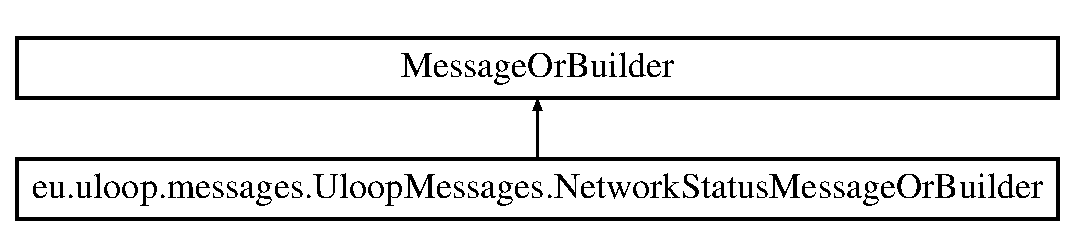
\includegraphics[height=2.000000cm]{interfaceeu_1_1uloop_1_1messages_1_1UloopMessages_1_1NetworkStatusMessageOrBuilder}
\end{center}
\end{figure}
\subsection*{Public Member Functions}
\begin{DoxyCompactItemize}
\item 
boolean \hyperlink{interfaceeu_1_1uloop_1_1messages_1_1UloopMessages_1_1NetworkStatusMessageOrBuilder_a74e77cbd33d0f2fda1d8c78b0248efcc}{has\+Nsrep} ()
\item 
eu.\+uloop.\+messages.\+Uloop\+Messages.\+Network\+Status\+Message\+Reply \hyperlink{interfaceeu_1_1uloop_1_1messages_1_1UloopMessages_1_1NetworkStatusMessageOrBuilder_a5b925124f09e2722f5ebc6ba428fbbed}{get\+Nsrep} ()
\item 
\hyperlink{interfaceeu_1_1uloop_1_1messages_1_1UloopMessages_1_1NetworkStatusMessageReplyOrBuilder}{eu.\+uloop.\+messages.\+Uloop\+Messages.\+Network\+Status\+Message\+Reply\+Or\+Builder} \hyperlink{interfaceeu_1_1uloop_1_1messages_1_1UloopMessages_1_1NetworkStatusMessageOrBuilder_aa3f823c5fd78b62694b14bd44273a94e}{get\+Nsrep\+Or\+Builder} ()
\end{DoxyCompactItemize}


\subsection{Member Function Documentation}
\hypertarget{interfaceeu_1_1uloop_1_1messages_1_1UloopMessages_1_1NetworkStatusMessageOrBuilder_a5b925124f09e2722f5ebc6ba428fbbed}{\index{eu\+::uloop\+::messages\+::\+Uloop\+Messages\+::\+Network\+Status\+Message\+Or\+Builder@{eu\+::uloop\+::messages\+::\+Uloop\+Messages\+::\+Network\+Status\+Message\+Or\+Builder}!get\+Nsrep@{get\+Nsrep}}
\index{get\+Nsrep@{get\+Nsrep}!eu\+::uloop\+::messages\+::\+Uloop\+Messages\+::\+Network\+Status\+Message\+Or\+Builder@{eu\+::uloop\+::messages\+::\+Uloop\+Messages\+::\+Network\+Status\+Message\+Or\+Builder}}
\subsubsection[{get\+Nsrep}]{\setlength{\rightskip}{0pt plus 5cm}eu.\+uloop.\+messages.\+Uloop\+Messages.\+Network\+Status\+Message\+Reply eu.\+uloop.\+messages.\+Uloop\+Messages.\+Network\+Status\+Message\+Or\+Builder.\+get\+Nsrep (
\begin{DoxyParamCaption}
{}
\end{DoxyParamCaption}
)}}\label{interfaceeu_1_1uloop_1_1messages_1_1UloopMessages_1_1NetworkStatusMessageOrBuilder_a5b925124f09e2722f5ebc6ba428fbbed}
\hypertarget{interfaceeu_1_1uloop_1_1messages_1_1UloopMessages_1_1NetworkStatusMessageOrBuilder_aa3f823c5fd78b62694b14bd44273a94e}{\index{eu\+::uloop\+::messages\+::\+Uloop\+Messages\+::\+Network\+Status\+Message\+Or\+Builder@{eu\+::uloop\+::messages\+::\+Uloop\+Messages\+::\+Network\+Status\+Message\+Or\+Builder}!get\+Nsrep\+Or\+Builder@{get\+Nsrep\+Or\+Builder}}
\index{get\+Nsrep\+Or\+Builder@{get\+Nsrep\+Or\+Builder}!eu\+::uloop\+::messages\+::\+Uloop\+Messages\+::\+Network\+Status\+Message\+Or\+Builder@{eu\+::uloop\+::messages\+::\+Uloop\+Messages\+::\+Network\+Status\+Message\+Or\+Builder}}
\subsubsection[{get\+Nsrep\+Or\+Builder}]{\setlength{\rightskip}{0pt plus 5cm}{\bf eu.\+uloop.\+messages.\+Uloop\+Messages.\+Network\+Status\+Message\+Reply\+Or\+Builder} eu.\+uloop.\+messages.\+Uloop\+Messages.\+Network\+Status\+Message\+Or\+Builder.\+get\+Nsrep\+Or\+Builder (
\begin{DoxyParamCaption}
{}
\end{DoxyParamCaption}
)}}\label{interfaceeu_1_1uloop_1_1messages_1_1UloopMessages_1_1NetworkStatusMessageOrBuilder_aa3f823c5fd78b62694b14bd44273a94e}
\hypertarget{interfaceeu_1_1uloop_1_1messages_1_1UloopMessages_1_1NetworkStatusMessageOrBuilder_a74e77cbd33d0f2fda1d8c78b0248efcc}{\index{eu\+::uloop\+::messages\+::\+Uloop\+Messages\+::\+Network\+Status\+Message\+Or\+Builder@{eu\+::uloop\+::messages\+::\+Uloop\+Messages\+::\+Network\+Status\+Message\+Or\+Builder}!has\+Nsrep@{has\+Nsrep}}
\index{has\+Nsrep@{has\+Nsrep}!eu\+::uloop\+::messages\+::\+Uloop\+Messages\+::\+Network\+Status\+Message\+Or\+Builder@{eu\+::uloop\+::messages\+::\+Uloop\+Messages\+::\+Network\+Status\+Message\+Or\+Builder}}
\subsubsection[{has\+Nsrep}]{\setlength{\rightskip}{0pt plus 5cm}boolean eu.\+uloop.\+messages.\+Uloop\+Messages.\+Network\+Status\+Message\+Or\+Builder.\+has\+Nsrep (
\begin{DoxyParamCaption}
{}
\end{DoxyParamCaption}
)}}\label{interfaceeu_1_1uloop_1_1messages_1_1UloopMessages_1_1NetworkStatusMessageOrBuilder_a74e77cbd33d0f2fda1d8c78b0248efcc}


The documentation for this interface was generated from the following file\+:\begin{DoxyCompactItemize}
\item 
src/eu/uloop/messages/\hyperlink{UloopMessages_8java}{Uloop\+Messages.\+java}\end{DoxyCompactItemize}

\hypertarget{interfaceeu_1_1uloop_1_1messages_1_1UloopMessages_1_1NetworkStatusMessageReplyOrBuilder}{\section{eu.\+uloop.\+messages.\+Uloop\+Messages.\+Network\+Status\+Message\+Reply\+Or\+Builder Interface Reference}
\label{interfaceeu_1_1uloop_1_1messages_1_1UloopMessages_1_1NetworkStatusMessageReplyOrBuilder}\index{eu.\+uloop.\+messages.\+Uloop\+Messages.\+Network\+Status\+Message\+Reply\+Or\+Builder@{eu.\+uloop.\+messages.\+Uloop\+Messages.\+Network\+Status\+Message\+Reply\+Or\+Builder}}
}
Inheritance diagram for eu.\+uloop.\+messages.\+Uloop\+Messages.\+Network\+Status\+Message\+Reply\+Or\+Builder\+:\begin{figure}[H]
\begin{center}
\leavevmode
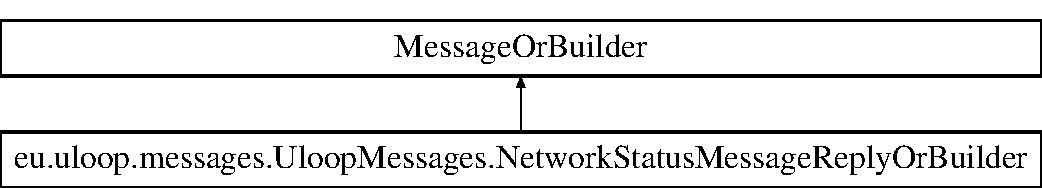
\includegraphics[height=2.000000cm]{interfaceeu_1_1uloop_1_1messages_1_1UloopMessages_1_1NetworkStatusMessageReplyOrBuilder}
\end{center}
\end{figure}
\subsection*{Public Member Functions}
\begin{DoxyCompactItemize}
\item 
boolean \hyperlink{interfaceeu_1_1uloop_1_1messages_1_1UloopMessages_1_1NetworkStatusMessageReplyOrBuilder_a0509c8ec0f76840337cb8b7ee5f2595b}{has\+Uplink} ()
\item 
long \hyperlink{interfaceeu_1_1uloop_1_1messages_1_1UloopMessages_1_1NetworkStatusMessageReplyOrBuilder_a556bcbf86c58885d8e1c48fc5173f3ff}{get\+Uplink} ()
\item 
boolean \hyperlink{interfaceeu_1_1uloop_1_1messages_1_1UloopMessages_1_1NetworkStatusMessageReplyOrBuilder_a204ce529f1f0f41b246fea62d5f993ab}{has\+Available} ()
\item 
long \hyperlink{interfaceeu_1_1uloop_1_1messages_1_1UloopMessages_1_1NetworkStatusMessageReplyOrBuilder_a4059b5bf18655f2f119a0d6c26cec204}{get\+Available} ()
\end{DoxyCompactItemize}


\subsection{Member Function Documentation}
\hypertarget{interfaceeu_1_1uloop_1_1messages_1_1UloopMessages_1_1NetworkStatusMessageReplyOrBuilder_a4059b5bf18655f2f119a0d6c26cec204}{\index{eu\+::uloop\+::messages\+::\+Uloop\+Messages\+::\+Network\+Status\+Message\+Reply\+Or\+Builder@{eu\+::uloop\+::messages\+::\+Uloop\+Messages\+::\+Network\+Status\+Message\+Reply\+Or\+Builder}!get\+Available@{get\+Available}}
\index{get\+Available@{get\+Available}!eu\+::uloop\+::messages\+::\+Uloop\+Messages\+::\+Network\+Status\+Message\+Reply\+Or\+Builder@{eu\+::uloop\+::messages\+::\+Uloop\+Messages\+::\+Network\+Status\+Message\+Reply\+Or\+Builder}}
\subsubsection[{get\+Available}]{\setlength{\rightskip}{0pt plus 5cm}long eu.\+uloop.\+messages.\+Uloop\+Messages.\+Network\+Status\+Message\+Reply\+Or\+Builder.\+get\+Available (
\begin{DoxyParamCaption}
{}
\end{DoxyParamCaption}
)}}\label{interfaceeu_1_1uloop_1_1messages_1_1UloopMessages_1_1NetworkStatusMessageReplyOrBuilder_a4059b5bf18655f2f119a0d6c26cec204}
\hypertarget{interfaceeu_1_1uloop_1_1messages_1_1UloopMessages_1_1NetworkStatusMessageReplyOrBuilder_a556bcbf86c58885d8e1c48fc5173f3ff}{\index{eu\+::uloop\+::messages\+::\+Uloop\+Messages\+::\+Network\+Status\+Message\+Reply\+Or\+Builder@{eu\+::uloop\+::messages\+::\+Uloop\+Messages\+::\+Network\+Status\+Message\+Reply\+Or\+Builder}!get\+Uplink@{get\+Uplink}}
\index{get\+Uplink@{get\+Uplink}!eu\+::uloop\+::messages\+::\+Uloop\+Messages\+::\+Network\+Status\+Message\+Reply\+Or\+Builder@{eu\+::uloop\+::messages\+::\+Uloop\+Messages\+::\+Network\+Status\+Message\+Reply\+Or\+Builder}}
\subsubsection[{get\+Uplink}]{\setlength{\rightskip}{0pt plus 5cm}long eu.\+uloop.\+messages.\+Uloop\+Messages.\+Network\+Status\+Message\+Reply\+Or\+Builder.\+get\+Uplink (
\begin{DoxyParamCaption}
{}
\end{DoxyParamCaption}
)}}\label{interfaceeu_1_1uloop_1_1messages_1_1UloopMessages_1_1NetworkStatusMessageReplyOrBuilder_a556bcbf86c58885d8e1c48fc5173f3ff}
\hypertarget{interfaceeu_1_1uloop_1_1messages_1_1UloopMessages_1_1NetworkStatusMessageReplyOrBuilder_a204ce529f1f0f41b246fea62d5f993ab}{\index{eu\+::uloop\+::messages\+::\+Uloop\+Messages\+::\+Network\+Status\+Message\+Reply\+Or\+Builder@{eu\+::uloop\+::messages\+::\+Uloop\+Messages\+::\+Network\+Status\+Message\+Reply\+Or\+Builder}!has\+Available@{has\+Available}}
\index{has\+Available@{has\+Available}!eu\+::uloop\+::messages\+::\+Uloop\+Messages\+::\+Network\+Status\+Message\+Reply\+Or\+Builder@{eu\+::uloop\+::messages\+::\+Uloop\+Messages\+::\+Network\+Status\+Message\+Reply\+Or\+Builder}}
\subsubsection[{has\+Available}]{\setlength{\rightskip}{0pt plus 5cm}boolean eu.\+uloop.\+messages.\+Uloop\+Messages.\+Network\+Status\+Message\+Reply\+Or\+Builder.\+has\+Available (
\begin{DoxyParamCaption}
{}
\end{DoxyParamCaption}
)}}\label{interfaceeu_1_1uloop_1_1messages_1_1UloopMessages_1_1NetworkStatusMessageReplyOrBuilder_a204ce529f1f0f41b246fea62d5f993ab}
\hypertarget{interfaceeu_1_1uloop_1_1messages_1_1UloopMessages_1_1NetworkStatusMessageReplyOrBuilder_a0509c8ec0f76840337cb8b7ee5f2595b}{\index{eu\+::uloop\+::messages\+::\+Uloop\+Messages\+::\+Network\+Status\+Message\+Reply\+Or\+Builder@{eu\+::uloop\+::messages\+::\+Uloop\+Messages\+::\+Network\+Status\+Message\+Reply\+Or\+Builder}!has\+Uplink@{has\+Uplink}}
\index{has\+Uplink@{has\+Uplink}!eu\+::uloop\+::messages\+::\+Uloop\+Messages\+::\+Network\+Status\+Message\+Reply\+Or\+Builder@{eu\+::uloop\+::messages\+::\+Uloop\+Messages\+::\+Network\+Status\+Message\+Reply\+Or\+Builder}}
\subsubsection[{has\+Uplink}]{\setlength{\rightskip}{0pt plus 5cm}boolean eu.\+uloop.\+messages.\+Uloop\+Messages.\+Network\+Status\+Message\+Reply\+Or\+Builder.\+has\+Uplink (
\begin{DoxyParamCaption}
{}
\end{DoxyParamCaption}
)}}\label{interfaceeu_1_1uloop_1_1messages_1_1UloopMessages_1_1NetworkStatusMessageReplyOrBuilder_a0509c8ec0f76840337cb8b7ee5f2595b}


The documentation for this interface was generated from the following file\+:\begin{DoxyCompactItemize}
\item 
src/eu/uloop/messages/\hyperlink{UloopMessages_8java}{Uloop\+Messages.\+java}\end{DoxyCompactItemize}

\hypertarget{interfaceeu_1_1uloop_1_1messages_1_1UloopMessages_1_1NewUserDetailsMessageOrBuilder}{\section{eu.\+uloop.\+messages.\+Uloop\+Messages.\+New\+User\+Details\+Message\+Or\+Builder Interface Reference}
\label{interfaceeu_1_1uloop_1_1messages_1_1UloopMessages_1_1NewUserDetailsMessageOrBuilder}\index{eu.\+uloop.\+messages.\+Uloop\+Messages.\+New\+User\+Details\+Message\+Or\+Builder@{eu.\+uloop.\+messages.\+Uloop\+Messages.\+New\+User\+Details\+Message\+Or\+Builder}}
}
Inheritance diagram for eu.\+uloop.\+messages.\+Uloop\+Messages.\+New\+User\+Details\+Message\+Or\+Builder\+:\begin{figure}[H]
\begin{center}
\leavevmode
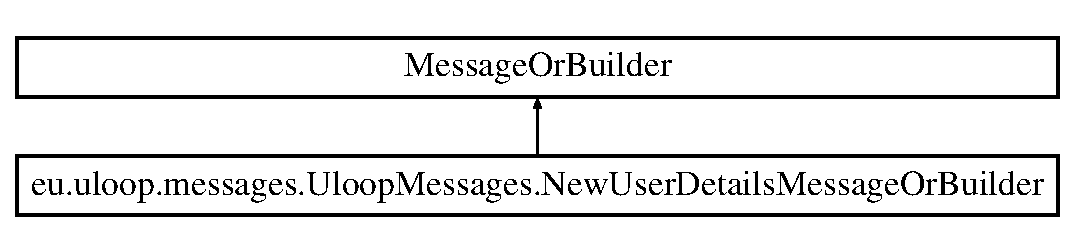
\includegraphics[height=2.000000cm]{interfaceeu_1_1uloop_1_1messages_1_1UloopMessages_1_1NewUserDetailsMessageOrBuilder}
\end{center}
\end{figure}
\subsection*{Public Member Functions}
\begin{DoxyCompactItemize}
\item 
boolean \hyperlink{interfaceeu_1_1uloop_1_1messages_1_1UloopMessages_1_1NewUserDetailsMessageOrBuilder_a9fcf0b3404d306058652c2531c20ff76}{has\+Cryptoid} ()
\item 
com.\+google.\+protobuf.\+Byte\+String \hyperlink{interfaceeu_1_1uloop_1_1messages_1_1UloopMessages_1_1NewUserDetailsMessageOrBuilder_a395174043045e6c69d20c473d5e0218b}{get\+Cryptoid} ()
\item 
boolean \hyperlink{interfaceeu_1_1uloop_1_1messages_1_1UloopMessages_1_1NewUserDetailsMessageOrBuilder_a93e9d6e417c4971a2ce7b6d246f0fcb2}{has\+Token} ()
\item 
double \hyperlink{interfaceeu_1_1uloop_1_1messages_1_1UloopMessages_1_1NewUserDetailsMessageOrBuilder_a3cbd6ee88ca68476373a457d35b743a7}{get\+Token} ()
\end{DoxyCompactItemize}


\subsection{Member Function Documentation}
\hypertarget{interfaceeu_1_1uloop_1_1messages_1_1UloopMessages_1_1NewUserDetailsMessageOrBuilder_a395174043045e6c69d20c473d5e0218b}{\index{eu\+::uloop\+::messages\+::\+Uloop\+Messages\+::\+New\+User\+Details\+Message\+Or\+Builder@{eu\+::uloop\+::messages\+::\+Uloop\+Messages\+::\+New\+User\+Details\+Message\+Or\+Builder}!get\+Cryptoid@{get\+Cryptoid}}
\index{get\+Cryptoid@{get\+Cryptoid}!eu\+::uloop\+::messages\+::\+Uloop\+Messages\+::\+New\+User\+Details\+Message\+Or\+Builder@{eu\+::uloop\+::messages\+::\+Uloop\+Messages\+::\+New\+User\+Details\+Message\+Or\+Builder}}
\subsubsection[{get\+Cryptoid}]{\setlength{\rightskip}{0pt plus 5cm}com.\+google.\+protobuf.\+Byte\+String eu.\+uloop.\+messages.\+Uloop\+Messages.\+New\+User\+Details\+Message\+Or\+Builder.\+get\+Cryptoid (
\begin{DoxyParamCaption}
{}
\end{DoxyParamCaption}
)}}\label{interfaceeu_1_1uloop_1_1messages_1_1UloopMessages_1_1NewUserDetailsMessageOrBuilder_a395174043045e6c69d20c473d5e0218b}
\hypertarget{interfaceeu_1_1uloop_1_1messages_1_1UloopMessages_1_1NewUserDetailsMessageOrBuilder_a3cbd6ee88ca68476373a457d35b743a7}{\index{eu\+::uloop\+::messages\+::\+Uloop\+Messages\+::\+New\+User\+Details\+Message\+Or\+Builder@{eu\+::uloop\+::messages\+::\+Uloop\+Messages\+::\+New\+User\+Details\+Message\+Or\+Builder}!get\+Token@{get\+Token}}
\index{get\+Token@{get\+Token}!eu\+::uloop\+::messages\+::\+Uloop\+Messages\+::\+New\+User\+Details\+Message\+Or\+Builder@{eu\+::uloop\+::messages\+::\+Uloop\+Messages\+::\+New\+User\+Details\+Message\+Or\+Builder}}
\subsubsection[{get\+Token}]{\setlength{\rightskip}{0pt plus 5cm}double eu.\+uloop.\+messages.\+Uloop\+Messages.\+New\+User\+Details\+Message\+Or\+Builder.\+get\+Token (
\begin{DoxyParamCaption}
{}
\end{DoxyParamCaption}
)}}\label{interfaceeu_1_1uloop_1_1messages_1_1UloopMessages_1_1NewUserDetailsMessageOrBuilder_a3cbd6ee88ca68476373a457d35b743a7}
\hypertarget{interfaceeu_1_1uloop_1_1messages_1_1UloopMessages_1_1NewUserDetailsMessageOrBuilder_a9fcf0b3404d306058652c2531c20ff76}{\index{eu\+::uloop\+::messages\+::\+Uloop\+Messages\+::\+New\+User\+Details\+Message\+Or\+Builder@{eu\+::uloop\+::messages\+::\+Uloop\+Messages\+::\+New\+User\+Details\+Message\+Or\+Builder}!has\+Cryptoid@{has\+Cryptoid}}
\index{has\+Cryptoid@{has\+Cryptoid}!eu\+::uloop\+::messages\+::\+Uloop\+Messages\+::\+New\+User\+Details\+Message\+Or\+Builder@{eu\+::uloop\+::messages\+::\+Uloop\+Messages\+::\+New\+User\+Details\+Message\+Or\+Builder}}
\subsubsection[{has\+Cryptoid}]{\setlength{\rightskip}{0pt plus 5cm}boolean eu.\+uloop.\+messages.\+Uloop\+Messages.\+New\+User\+Details\+Message\+Or\+Builder.\+has\+Cryptoid (
\begin{DoxyParamCaption}
{}
\end{DoxyParamCaption}
)}}\label{interfaceeu_1_1uloop_1_1messages_1_1UloopMessages_1_1NewUserDetailsMessageOrBuilder_a9fcf0b3404d306058652c2531c20ff76}
\hypertarget{interfaceeu_1_1uloop_1_1messages_1_1UloopMessages_1_1NewUserDetailsMessageOrBuilder_a93e9d6e417c4971a2ce7b6d246f0fcb2}{\index{eu\+::uloop\+::messages\+::\+Uloop\+Messages\+::\+New\+User\+Details\+Message\+Or\+Builder@{eu\+::uloop\+::messages\+::\+Uloop\+Messages\+::\+New\+User\+Details\+Message\+Or\+Builder}!has\+Token@{has\+Token}}
\index{has\+Token@{has\+Token}!eu\+::uloop\+::messages\+::\+Uloop\+Messages\+::\+New\+User\+Details\+Message\+Or\+Builder@{eu\+::uloop\+::messages\+::\+Uloop\+Messages\+::\+New\+User\+Details\+Message\+Or\+Builder}}
\subsubsection[{has\+Token}]{\setlength{\rightskip}{0pt plus 5cm}boolean eu.\+uloop.\+messages.\+Uloop\+Messages.\+New\+User\+Details\+Message\+Or\+Builder.\+has\+Token (
\begin{DoxyParamCaption}
{}
\end{DoxyParamCaption}
)}}\label{interfaceeu_1_1uloop_1_1messages_1_1UloopMessages_1_1NewUserDetailsMessageOrBuilder_a93e9d6e417c4971a2ce7b6d246f0fcb2}


The documentation for this interface was generated from the following file\+:\begin{DoxyCompactItemize}
\item 
src/eu/uloop/messages/\hyperlink{UloopMessages_8java}{Uloop\+Messages.\+java}\end{DoxyCompactItemize}

\hypertarget{interfaceeu_1_1uloop_1_1messages_1_1UloopMessages_1_1QoSMessageOrBuilder}{\section{eu.\+uloop.\+messages.\+Uloop\+Messages.\+Qo\+S\+Message\+Or\+Builder Interface Reference}
\label{interfaceeu_1_1uloop_1_1messages_1_1UloopMessages_1_1QoSMessageOrBuilder}\index{eu.\+uloop.\+messages.\+Uloop\+Messages.\+Qo\+S\+Message\+Or\+Builder@{eu.\+uloop.\+messages.\+Uloop\+Messages.\+Qo\+S\+Message\+Or\+Builder}}
}
Inheritance diagram for eu.\+uloop.\+messages.\+Uloop\+Messages.\+Qo\+S\+Message\+Or\+Builder\+:\begin{figure}[H]
\begin{center}
\leavevmode
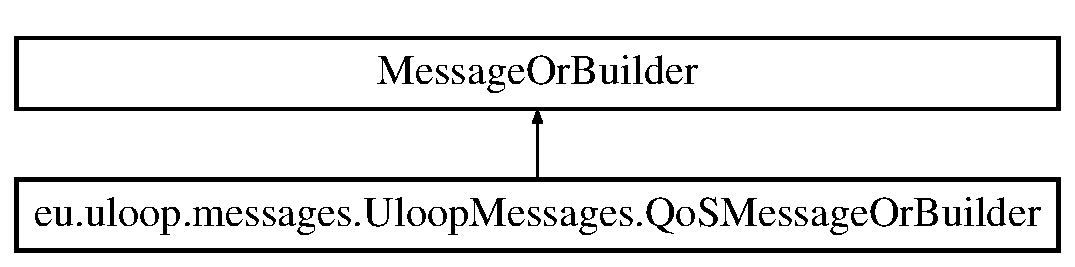
\includegraphics[height=2.000000cm]{interfaceeu_1_1uloop_1_1messages_1_1UloopMessages_1_1QoSMessageOrBuilder}
\end{center}
\end{figure}
\subsection*{Public Member Functions}
\begin{DoxyCompactItemize}
\item 
boolean \hyperlink{interfaceeu_1_1uloop_1_1messages_1_1UloopMessages_1_1QoSMessageOrBuilder_ae71c834c8de416f3abbf62c8068cc34b}{has\+Tuple} ()
\item 
eu.\+uloop.\+messages.\+Uloop\+Messages.\+Qo\+S\+Tuple \hyperlink{interfaceeu_1_1uloop_1_1messages_1_1UloopMessages_1_1QoSMessageOrBuilder_a2b85843bf8226e5de1c86a781b36f50e}{get\+Tuple} ()
\item 
\hyperlink{interfaceeu_1_1uloop_1_1messages_1_1UloopMessages_1_1QoSTupleOrBuilder}{eu.\+uloop.\+messages.\+Uloop\+Messages.\+Qo\+S\+Tuple\+Or\+Builder} \hyperlink{interfaceeu_1_1uloop_1_1messages_1_1UloopMessages_1_1QoSMessageOrBuilder_a7168aa65339f894276f11cb45fd53dd4}{get\+Tuple\+Or\+Builder} ()
\item 
boolean \hyperlink{interfaceeu_1_1uloop_1_1messages_1_1UloopMessages_1_1QoSMessageOrBuilder_a791f44dad5bc28b88db7d9f731a282b7}{has\+Req} ()
\item 
eu.\+uloop.\+messages.\+Uloop\+Messages.\+Qos\+Request \hyperlink{interfaceeu_1_1uloop_1_1messages_1_1UloopMessages_1_1QoSMessageOrBuilder_ab401d6931e2b348e25fc5c8656138245}{get\+Req} ()
\item 
\hyperlink{interfaceeu_1_1uloop_1_1messages_1_1UloopMessages_1_1QosRequestOrBuilder}{eu.\+uloop.\+messages.\+Uloop\+Messages.\+Qos\+Request\+Or\+Builder} \hyperlink{interfaceeu_1_1uloop_1_1messages_1_1UloopMessages_1_1QoSMessageOrBuilder_a38597d3c36d910f717a28502b0ce9ed5}{get\+Req\+Or\+Builder} ()
\end{DoxyCompactItemize}


\subsection{Member Function Documentation}
\hypertarget{interfaceeu_1_1uloop_1_1messages_1_1UloopMessages_1_1QoSMessageOrBuilder_ab401d6931e2b348e25fc5c8656138245}{\index{eu\+::uloop\+::messages\+::\+Uloop\+Messages\+::\+Qo\+S\+Message\+Or\+Builder@{eu\+::uloop\+::messages\+::\+Uloop\+Messages\+::\+Qo\+S\+Message\+Or\+Builder}!get\+Req@{get\+Req}}
\index{get\+Req@{get\+Req}!eu\+::uloop\+::messages\+::\+Uloop\+Messages\+::\+Qo\+S\+Message\+Or\+Builder@{eu\+::uloop\+::messages\+::\+Uloop\+Messages\+::\+Qo\+S\+Message\+Or\+Builder}}
\subsubsection[{get\+Req}]{\setlength{\rightskip}{0pt plus 5cm}eu.\+uloop.\+messages.\+Uloop\+Messages.\+Qos\+Request eu.\+uloop.\+messages.\+Uloop\+Messages.\+Qo\+S\+Message\+Or\+Builder.\+get\+Req (
\begin{DoxyParamCaption}
{}
\end{DoxyParamCaption}
)}}\label{interfaceeu_1_1uloop_1_1messages_1_1UloopMessages_1_1QoSMessageOrBuilder_ab401d6931e2b348e25fc5c8656138245}
\hypertarget{interfaceeu_1_1uloop_1_1messages_1_1UloopMessages_1_1QoSMessageOrBuilder_a38597d3c36d910f717a28502b0ce9ed5}{\index{eu\+::uloop\+::messages\+::\+Uloop\+Messages\+::\+Qo\+S\+Message\+Or\+Builder@{eu\+::uloop\+::messages\+::\+Uloop\+Messages\+::\+Qo\+S\+Message\+Or\+Builder}!get\+Req\+Or\+Builder@{get\+Req\+Or\+Builder}}
\index{get\+Req\+Or\+Builder@{get\+Req\+Or\+Builder}!eu\+::uloop\+::messages\+::\+Uloop\+Messages\+::\+Qo\+S\+Message\+Or\+Builder@{eu\+::uloop\+::messages\+::\+Uloop\+Messages\+::\+Qo\+S\+Message\+Or\+Builder}}
\subsubsection[{get\+Req\+Or\+Builder}]{\setlength{\rightskip}{0pt plus 5cm}{\bf eu.\+uloop.\+messages.\+Uloop\+Messages.\+Qos\+Request\+Or\+Builder} eu.\+uloop.\+messages.\+Uloop\+Messages.\+Qo\+S\+Message\+Or\+Builder.\+get\+Req\+Or\+Builder (
\begin{DoxyParamCaption}
{}
\end{DoxyParamCaption}
)}}\label{interfaceeu_1_1uloop_1_1messages_1_1UloopMessages_1_1QoSMessageOrBuilder_a38597d3c36d910f717a28502b0ce9ed5}
\hypertarget{interfaceeu_1_1uloop_1_1messages_1_1UloopMessages_1_1QoSMessageOrBuilder_a2b85843bf8226e5de1c86a781b36f50e}{\index{eu\+::uloop\+::messages\+::\+Uloop\+Messages\+::\+Qo\+S\+Message\+Or\+Builder@{eu\+::uloop\+::messages\+::\+Uloop\+Messages\+::\+Qo\+S\+Message\+Or\+Builder}!get\+Tuple@{get\+Tuple}}
\index{get\+Tuple@{get\+Tuple}!eu\+::uloop\+::messages\+::\+Uloop\+Messages\+::\+Qo\+S\+Message\+Or\+Builder@{eu\+::uloop\+::messages\+::\+Uloop\+Messages\+::\+Qo\+S\+Message\+Or\+Builder}}
\subsubsection[{get\+Tuple}]{\setlength{\rightskip}{0pt plus 5cm}eu.\+uloop.\+messages.\+Uloop\+Messages.\+Qo\+S\+Tuple eu.\+uloop.\+messages.\+Uloop\+Messages.\+Qo\+S\+Message\+Or\+Builder.\+get\+Tuple (
\begin{DoxyParamCaption}
{}
\end{DoxyParamCaption}
)}}\label{interfaceeu_1_1uloop_1_1messages_1_1UloopMessages_1_1QoSMessageOrBuilder_a2b85843bf8226e5de1c86a781b36f50e}
\hypertarget{interfaceeu_1_1uloop_1_1messages_1_1UloopMessages_1_1QoSMessageOrBuilder_a7168aa65339f894276f11cb45fd53dd4}{\index{eu\+::uloop\+::messages\+::\+Uloop\+Messages\+::\+Qo\+S\+Message\+Or\+Builder@{eu\+::uloop\+::messages\+::\+Uloop\+Messages\+::\+Qo\+S\+Message\+Or\+Builder}!get\+Tuple\+Or\+Builder@{get\+Tuple\+Or\+Builder}}
\index{get\+Tuple\+Or\+Builder@{get\+Tuple\+Or\+Builder}!eu\+::uloop\+::messages\+::\+Uloop\+Messages\+::\+Qo\+S\+Message\+Or\+Builder@{eu\+::uloop\+::messages\+::\+Uloop\+Messages\+::\+Qo\+S\+Message\+Or\+Builder}}
\subsubsection[{get\+Tuple\+Or\+Builder}]{\setlength{\rightskip}{0pt plus 5cm}{\bf eu.\+uloop.\+messages.\+Uloop\+Messages.\+Qo\+S\+Tuple\+Or\+Builder} eu.\+uloop.\+messages.\+Uloop\+Messages.\+Qo\+S\+Message\+Or\+Builder.\+get\+Tuple\+Or\+Builder (
\begin{DoxyParamCaption}
{}
\end{DoxyParamCaption}
)}}\label{interfaceeu_1_1uloop_1_1messages_1_1UloopMessages_1_1QoSMessageOrBuilder_a7168aa65339f894276f11cb45fd53dd4}
\hypertarget{interfaceeu_1_1uloop_1_1messages_1_1UloopMessages_1_1QoSMessageOrBuilder_a791f44dad5bc28b88db7d9f731a282b7}{\index{eu\+::uloop\+::messages\+::\+Uloop\+Messages\+::\+Qo\+S\+Message\+Or\+Builder@{eu\+::uloop\+::messages\+::\+Uloop\+Messages\+::\+Qo\+S\+Message\+Or\+Builder}!has\+Req@{has\+Req}}
\index{has\+Req@{has\+Req}!eu\+::uloop\+::messages\+::\+Uloop\+Messages\+::\+Qo\+S\+Message\+Or\+Builder@{eu\+::uloop\+::messages\+::\+Uloop\+Messages\+::\+Qo\+S\+Message\+Or\+Builder}}
\subsubsection[{has\+Req}]{\setlength{\rightskip}{0pt plus 5cm}boolean eu.\+uloop.\+messages.\+Uloop\+Messages.\+Qo\+S\+Message\+Or\+Builder.\+has\+Req (
\begin{DoxyParamCaption}
{}
\end{DoxyParamCaption}
)}}\label{interfaceeu_1_1uloop_1_1messages_1_1UloopMessages_1_1QoSMessageOrBuilder_a791f44dad5bc28b88db7d9f731a282b7}
\hypertarget{interfaceeu_1_1uloop_1_1messages_1_1UloopMessages_1_1QoSMessageOrBuilder_ae71c834c8de416f3abbf62c8068cc34b}{\index{eu\+::uloop\+::messages\+::\+Uloop\+Messages\+::\+Qo\+S\+Message\+Or\+Builder@{eu\+::uloop\+::messages\+::\+Uloop\+Messages\+::\+Qo\+S\+Message\+Or\+Builder}!has\+Tuple@{has\+Tuple}}
\index{has\+Tuple@{has\+Tuple}!eu\+::uloop\+::messages\+::\+Uloop\+Messages\+::\+Qo\+S\+Message\+Or\+Builder@{eu\+::uloop\+::messages\+::\+Uloop\+Messages\+::\+Qo\+S\+Message\+Or\+Builder}}
\subsubsection[{has\+Tuple}]{\setlength{\rightskip}{0pt plus 5cm}boolean eu.\+uloop.\+messages.\+Uloop\+Messages.\+Qo\+S\+Message\+Or\+Builder.\+has\+Tuple (
\begin{DoxyParamCaption}
{}
\end{DoxyParamCaption}
)}}\label{interfaceeu_1_1uloop_1_1messages_1_1UloopMessages_1_1QoSMessageOrBuilder_ae71c834c8de416f3abbf62c8068cc34b}


The documentation for this interface was generated from the following file\+:\begin{DoxyCompactItemize}
\item 
src/eu/uloop/messages/\hyperlink{UloopMessages_8java}{Uloop\+Messages.\+java}\end{DoxyCompactItemize}

\hypertarget{interfaceeu_1_1uloop_1_1messages_1_1UloopMessages_1_1QosRequestOrBuilder}{\section{eu.\+uloop.\+messages.\+Uloop\+Messages.\+Qos\+Request\+Or\+Builder Interface Reference}
\label{interfaceeu_1_1uloop_1_1messages_1_1UloopMessages_1_1QosRequestOrBuilder}\index{eu.\+uloop.\+messages.\+Uloop\+Messages.\+Qos\+Request\+Or\+Builder@{eu.\+uloop.\+messages.\+Uloop\+Messages.\+Qos\+Request\+Or\+Builder}}
}
Inheritance diagram for eu.\+uloop.\+messages.\+Uloop\+Messages.\+Qos\+Request\+Or\+Builder\+:\begin{figure}[H]
\begin{center}
\leavevmode
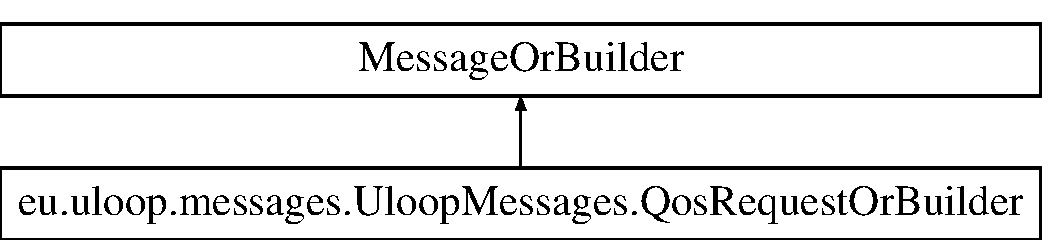
\includegraphics[height=2.000000cm]{interfaceeu_1_1uloop_1_1messages_1_1UloopMessages_1_1QosRequestOrBuilder}
\end{center}
\end{figure}
\subsection*{Public Member Functions}
\begin{DoxyCompactItemize}
\item 
boolean \hyperlink{interfaceeu_1_1uloop_1_1messages_1_1UloopMessages_1_1QosRequestOrBuilder_a236f0e4de792b3ca6abe00e92be133b6}{has\+Request} ()
\item 
String \hyperlink{interfaceeu_1_1uloop_1_1messages_1_1UloopMessages_1_1QosRequestOrBuilder_a208aa64ba9ab3d09f588527485bec93b}{get\+Request} ()
\end{DoxyCompactItemize}


\subsection{Member Function Documentation}
\hypertarget{interfaceeu_1_1uloop_1_1messages_1_1UloopMessages_1_1QosRequestOrBuilder_a208aa64ba9ab3d09f588527485bec93b}{\index{eu\+::uloop\+::messages\+::\+Uloop\+Messages\+::\+Qos\+Request\+Or\+Builder@{eu\+::uloop\+::messages\+::\+Uloop\+Messages\+::\+Qos\+Request\+Or\+Builder}!get\+Request@{get\+Request}}
\index{get\+Request@{get\+Request}!eu\+::uloop\+::messages\+::\+Uloop\+Messages\+::\+Qos\+Request\+Or\+Builder@{eu\+::uloop\+::messages\+::\+Uloop\+Messages\+::\+Qos\+Request\+Or\+Builder}}
\subsubsection[{get\+Request}]{\setlength{\rightskip}{0pt plus 5cm}String eu.\+uloop.\+messages.\+Uloop\+Messages.\+Qos\+Request\+Or\+Builder.\+get\+Request (
\begin{DoxyParamCaption}
{}
\end{DoxyParamCaption}
)}}\label{interfaceeu_1_1uloop_1_1messages_1_1UloopMessages_1_1QosRequestOrBuilder_a208aa64ba9ab3d09f588527485bec93b}
\hypertarget{interfaceeu_1_1uloop_1_1messages_1_1UloopMessages_1_1QosRequestOrBuilder_a236f0e4de792b3ca6abe00e92be133b6}{\index{eu\+::uloop\+::messages\+::\+Uloop\+Messages\+::\+Qos\+Request\+Or\+Builder@{eu\+::uloop\+::messages\+::\+Uloop\+Messages\+::\+Qos\+Request\+Or\+Builder}!has\+Request@{has\+Request}}
\index{has\+Request@{has\+Request}!eu\+::uloop\+::messages\+::\+Uloop\+Messages\+::\+Qos\+Request\+Or\+Builder@{eu\+::uloop\+::messages\+::\+Uloop\+Messages\+::\+Qos\+Request\+Or\+Builder}}
\subsubsection[{has\+Request}]{\setlength{\rightskip}{0pt plus 5cm}boolean eu.\+uloop.\+messages.\+Uloop\+Messages.\+Qos\+Request\+Or\+Builder.\+has\+Request (
\begin{DoxyParamCaption}
{}
\end{DoxyParamCaption}
)}}\label{interfaceeu_1_1uloop_1_1messages_1_1UloopMessages_1_1QosRequestOrBuilder_a236f0e4de792b3ca6abe00e92be133b6}


The documentation for this interface was generated from the following file\+:\begin{DoxyCompactItemize}
\item 
src/eu/uloop/messages/\hyperlink{UloopMessages_8java}{Uloop\+Messages.\+java}\end{DoxyCompactItemize}

\hypertarget{interfaceeu_1_1uloop_1_1messages_1_1UloopMessages_1_1QoSTupleOrBuilder}{\section{eu.\+uloop.\+messages.\+Uloop\+Messages.\+Qo\+S\+Tuple\+Or\+Builder Interface Reference}
\label{interfaceeu_1_1uloop_1_1messages_1_1UloopMessages_1_1QoSTupleOrBuilder}\index{eu.\+uloop.\+messages.\+Uloop\+Messages.\+Qo\+S\+Tuple\+Or\+Builder@{eu.\+uloop.\+messages.\+Uloop\+Messages.\+Qo\+S\+Tuple\+Or\+Builder}}
}
Inheritance diagram for eu.\+uloop.\+messages.\+Uloop\+Messages.\+Qo\+S\+Tuple\+Or\+Builder\+:\begin{figure}[H]
\begin{center}
\leavevmode
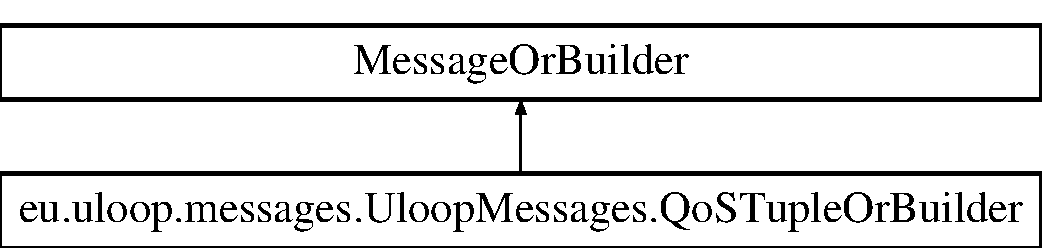
\includegraphics[height=2.000000cm]{interfaceeu_1_1uloop_1_1messages_1_1UloopMessages_1_1QoSTupleOrBuilder}
\end{center}
\end{figure}
\subsection*{Public Member Functions}
\begin{DoxyCompactItemize}
\item 
boolean \hyperlink{interfaceeu_1_1uloop_1_1messages_1_1UloopMessages_1_1QoSTupleOrBuilder_ab56b77a9f4d9cc5fac7e710e99d5674d}{has\+Client\+I\+P} ()
\item 
String \hyperlink{interfaceeu_1_1uloop_1_1messages_1_1UloopMessages_1_1QoSTupleOrBuilder_af48c0a759e704ac0ea0fd0b9d64aae82}{get\+Client\+I\+P} ()
\item 
boolean \hyperlink{interfaceeu_1_1uloop_1_1messages_1_1UloopMessages_1_1QoSTupleOrBuilder_a2bf7ab0dd8a177509005a9217a23cf74}{has\+Avgdelay} ()
\item 
String \hyperlink{interfaceeu_1_1uloop_1_1messages_1_1UloopMessages_1_1QoSTupleOrBuilder_a989f8386f15cc0f4b0138c59a39d5b6a}{get\+Avgdelay} ()
\item 
boolean \hyperlink{interfaceeu_1_1uloop_1_1messages_1_1UloopMessages_1_1QoSTupleOrBuilder_a6dc82d0fa2db349759b84676b04ecd79}{has\+Avgbitrate} ()
\item 
String \hyperlink{interfaceeu_1_1uloop_1_1messages_1_1UloopMessages_1_1QoSTupleOrBuilder_acf9d5440ff0ea4db942f6a6ce6df5678}{get\+Avgbitrate} ()
\item 
boolean \hyperlink{interfaceeu_1_1uloop_1_1messages_1_1UloopMessages_1_1QoSTupleOrBuilder_abecabf3cd36e2cba3572936a5880a8ed}{has\+Avgpktloss} ()
\item 
String \hyperlink{interfaceeu_1_1uloop_1_1messages_1_1UloopMessages_1_1QoSTupleOrBuilder_ac2c04e5619c1efd111fbde91a523bdb4}{get\+Avgpktloss} ()
\item 
boolean \hyperlink{interfaceeu_1_1uloop_1_1messages_1_1UloopMessages_1_1QoSTupleOrBuilder_a6ea9de6501ab8166fe66b50996ed649d}{has\+Avgjitter} ()
\item 
String \hyperlink{interfaceeu_1_1uloop_1_1messages_1_1UloopMessages_1_1QoSTupleOrBuilder_a8bd7a434c087c9cf82fe1383b6d8123b}{get\+Avgjitter} ()
\end{DoxyCompactItemize}


\subsection{Member Function Documentation}
\hypertarget{interfaceeu_1_1uloop_1_1messages_1_1UloopMessages_1_1QoSTupleOrBuilder_acf9d5440ff0ea4db942f6a6ce6df5678}{\index{eu\+::uloop\+::messages\+::\+Uloop\+Messages\+::\+Qo\+S\+Tuple\+Or\+Builder@{eu\+::uloop\+::messages\+::\+Uloop\+Messages\+::\+Qo\+S\+Tuple\+Or\+Builder}!get\+Avgbitrate@{get\+Avgbitrate}}
\index{get\+Avgbitrate@{get\+Avgbitrate}!eu\+::uloop\+::messages\+::\+Uloop\+Messages\+::\+Qo\+S\+Tuple\+Or\+Builder@{eu\+::uloop\+::messages\+::\+Uloop\+Messages\+::\+Qo\+S\+Tuple\+Or\+Builder}}
\subsubsection[{get\+Avgbitrate}]{\setlength{\rightskip}{0pt plus 5cm}String eu.\+uloop.\+messages.\+Uloop\+Messages.\+Qo\+S\+Tuple\+Or\+Builder.\+get\+Avgbitrate (
\begin{DoxyParamCaption}
{}
\end{DoxyParamCaption}
)}}\label{interfaceeu_1_1uloop_1_1messages_1_1UloopMessages_1_1QoSTupleOrBuilder_acf9d5440ff0ea4db942f6a6ce6df5678}
\hypertarget{interfaceeu_1_1uloop_1_1messages_1_1UloopMessages_1_1QoSTupleOrBuilder_a989f8386f15cc0f4b0138c59a39d5b6a}{\index{eu\+::uloop\+::messages\+::\+Uloop\+Messages\+::\+Qo\+S\+Tuple\+Or\+Builder@{eu\+::uloop\+::messages\+::\+Uloop\+Messages\+::\+Qo\+S\+Tuple\+Or\+Builder}!get\+Avgdelay@{get\+Avgdelay}}
\index{get\+Avgdelay@{get\+Avgdelay}!eu\+::uloop\+::messages\+::\+Uloop\+Messages\+::\+Qo\+S\+Tuple\+Or\+Builder@{eu\+::uloop\+::messages\+::\+Uloop\+Messages\+::\+Qo\+S\+Tuple\+Or\+Builder}}
\subsubsection[{get\+Avgdelay}]{\setlength{\rightskip}{0pt plus 5cm}String eu.\+uloop.\+messages.\+Uloop\+Messages.\+Qo\+S\+Tuple\+Or\+Builder.\+get\+Avgdelay (
\begin{DoxyParamCaption}
{}
\end{DoxyParamCaption}
)}}\label{interfaceeu_1_1uloop_1_1messages_1_1UloopMessages_1_1QoSTupleOrBuilder_a989f8386f15cc0f4b0138c59a39d5b6a}
\hypertarget{interfaceeu_1_1uloop_1_1messages_1_1UloopMessages_1_1QoSTupleOrBuilder_a8bd7a434c087c9cf82fe1383b6d8123b}{\index{eu\+::uloop\+::messages\+::\+Uloop\+Messages\+::\+Qo\+S\+Tuple\+Or\+Builder@{eu\+::uloop\+::messages\+::\+Uloop\+Messages\+::\+Qo\+S\+Tuple\+Or\+Builder}!get\+Avgjitter@{get\+Avgjitter}}
\index{get\+Avgjitter@{get\+Avgjitter}!eu\+::uloop\+::messages\+::\+Uloop\+Messages\+::\+Qo\+S\+Tuple\+Or\+Builder@{eu\+::uloop\+::messages\+::\+Uloop\+Messages\+::\+Qo\+S\+Tuple\+Or\+Builder}}
\subsubsection[{get\+Avgjitter}]{\setlength{\rightskip}{0pt plus 5cm}String eu.\+uloop.\+messages.\+Uloop\+Messages.\+Qo\+S\+Tuple\+Or\+Builder.\+get\+Avgjitter (
\begin{DoxyParamCaption}
{}
\end{DoxyParamCaption}
)}}\label{interfaceeu_1_1uloop_1_1messages_1_1UloopMessages_1_1QoSTupleOrBuilder_a8bd7a434c087c9cf82fe1383b6d8123b}
\hypertarget{interfaceeu_1_1uloop_1_1messages_1_1UloopMessages_1_1QoSTupleOrBuilder_ac2c04e5619c1efd111fbde91a523bdb4}{\index{eu\+::uloop\+::messages\+::\+Uloop\+Messages\+::\+Qo\+S\+Tuple\+Or\+Builder@{eu\+::uloop\+::messages\+::\+Uloop\+Messages\+::\+Qo\+S\+Tuple\+Or\+Builder}!get\+Avgpktloss@{get\+Avgpktloss}}
\index{get\+Avgpktloss@{get\+Avgpktloss}!eu\+::uloop\+::messages\+::\+Uloop\+Messages\+::\+Qo\+S\+Tuple\+Or\+Builder@{eu\+::uloop\+::messages\+::\+Uloop\+Messages\+::\+Qo\+S\+Tuple\+Or\+Builder}}
\subsubsection[{get\+Avgpktloss}]{\setlength{\rightskip}{0pt plus 5cm}String eu.\+uloop.\+messages.\+Uloop\+Messages.\+Qo\+S\+Tuple\+Or\+Builder.\+get\+Avgpktloss (
\begin{DoxyParamCaption}
{}
\end{DoxyParamCaption}
)}}\label{interfaceeu_1_1uloop_1_1messages_1_1UloopMessages_1_1QoSTupleOrBuilder_ac2c04e5619c1efd111fbde91a523bdb4}
\hypertarget{interfaceeu_1_1uloop_1_1messages_1_1UloopMessages_1_1QoSTupleOrBuilder_af48c0a759e704ac0ea0fd0b9d64aae82}{\index{eu\+::uloop\+::messages\+::\+Uloop\+Messages\+::\+Qo\+S\+Tuple\+Or\+Builder@{eu\+::uloop\+::messages\+::\+Uloop\+Messages\+::\+Qo\+S\+Tuple\+Or\+Builder}!get\+Client\+I\+P@{get\+Client\+I\+P}}
\index{get\+Client\+I\+P@{get\+Client\+I\+P}!eu\+::uloop\+::messages\+::\+Uloop\+Messages\+::\+Qo\+S\+Tuple\+Or\+Builder@{eu\+::uloop\+::messages\+::\+Uloop\+Messages\+::\+Qo\+S\+Tuple\+Or\+Builder}}
\subsubsection[{get\+Client\+I\+P}]{\setlength{\rightskip}{0pt plus 5cm}String eu.\+uloop.\+messages.\+Uloop\+Messages.\+Qo\+S\+Tuple\+Or\+Builder.\+get\+Client\+I\+P (
\begin{DoxyParamCaption}
{}
\end{DoxyParamCaption}
)}}\label{interfaceeu_1_1uloop_1_1messages_1_1UloopMessages_1_1QoSTupleOrBuilder_af48c0a759e704ac0ea0fd0b9d64aae82}
\hypertarget{interfaceeu_1_1uloop_1_1messages_1_1UloopMessages_1_1QoSTupleOrBuilder_a6dc82d0fa2db349759b84676b04ecd79}{\index{eu\+::uloop\+::messages\+::\+Uloop\+Messages\+::\+Qo\+S\+Tuple\+Or\+Builder@{eu\+::uloop\+::messages\+::\+Uloop\+Messages\+::\+Qo\+S\+Tuple\+Or\+Builder}!has\+Avgbitrate@{has\+Avgbitrate}}
\index{has\+Avgbitrate@{has\+Avgbitrate}!eu\+::uloop\+::messages\+::\+Uloop\+Messages\+::\+Qo\+S\+Tuple\+Or\+Builder@{eu\+::uloop\+::messages\+::\+Uloop\+Messages\+::\+Qo\+S\+Tuple\+Or\+Builder}}
\subsubsection[{has\+Avgbitrate}]{\setlength{\rightskip}{0pt plus 5cm}boolean eu.\+uloop.\+messages.\+Uloop\+Messages.\+Qo\+S\+Tuple\+Or\+Builder.\+has\+Avgbitrate (
\begin{DoxyParamCaption}
{}
\end{DoxyParamCaption}
)}}\label{interfaceeu_1_1uloop_1_1messages_1_1UloopMessages_1_1QoSTupleOrBuilder_a6dc82d0fa2db349759b84676b04ecd79}
\hypertarget{interfaceeu_1_1uloop_1_1messages_1_1UloopMessages_1_1QoSTupleOrBuilder_a2bf7ab0dd8a177509005a9217a23cf74}{\index{eu\+::uloop\+::messages\+::\+Uloop\+Messages\+::\+Qo\+S\+Tuple\+Or\+Builder@{eu\+::uloop\+::messages\+::\+Uloop\+Messages\+::\+Qo\+S\+Tuple\+Or\+Builder}!has\+Avgdelay@{has\+Avgdelay}}
\index{has\+Avgdelay@{has\+Avgdelay}!eu\+::uloop\+::messages\+::\+Uloop\+Messages\+::\+Qo\+S\+Tuple\+Or\+Builder@{eu\+::uloop\+::messages\+::\+Uloop\+Messages\+::\+Qo\+S\+Tuple\+Or\+Builder}}
\subsubsection[{has\+Avgdelay}]{\setlength{\rightskip}{0pt plus 5cm}boolean eu.\+uloop.\+messages.\+Uloop\+Messages.\+Qo\+S\+Tuple\+Or\+Builder.\+has\+Avgdelay (
\begin{DoxyParamCaption}
{}
\end{DoxyParamCaption}
)}}\label{interfaceeu_1_1uloop_1_1messages_1_1UloopMessages_1_1QoSTupleOrBuilder_a2bf7ab0dd8a177509005a9217a23cf74}
\hypertarget{interfaceeu_1_1uloop_1_1messages_1_1UloopMessages_1_1QoSTupleOrBuilder_a6ea9de6501ab8166fe66b50996ed649d}{\index{eu\+::uloop\+::messages\+::\+Uloop\+Messages\+::\+Qo\+S\+Tuple\+Or\+Builder@{eu\+::uloop\+::messages\+::\+Uloop\+Messages\+::\+Qo\+S\+Tuple\+Or\+Builder}!has\+Avgjitter@{has\+Avgjitter}}
\index{has\+Avgjitter@{has\+Avgjitter}!eu\+::uloop\+::messages\+::\+Uloop\+Messages\+::\+Qo\+S\+Tuple\+Or\+Builder@{eu\+::uloop\+::messages\+::\+Uloop\+Messages\+::\+Qo\+S\+Tuple\+Or\+Builder}}
\subsubsection[{has\+Avgjitter}]{\setlength{\rightskip}{0pt plus 5cm}boolean eu.\+uloop.\+messages.\+Uloop\+Messages.\+Qo\+S\+Tuple\+Or\+Builder.\+has\+Avgjitter (
\begin{DoxyParamCaption}
{}
\end{DoxyParamCaption}
)}}\label{interfaceeu_1_1uloop_1_1messages_1_1UloopMessages_1_1QoSTupleOrBuilder_a6ea9de6501ab8166fe66b50996ed649d}
\hypertarget{interfaceeu_1_1uloop_1_1messages_1_1UloopMessages_1_1QoSTupleOrBuilder_abecabf3cd36e2cba3572936a5880a8ed}{\index{eu\+::uloop\+::messages\+::\+Uloop\+Messages\+::\+Qo\+S\+Tuple\+Or\+Builder@{eu\+::uloop\+::messages\+::\+Uloop\+Messages\+::\+Qo\+S\+Tuple\+Or\+Builder}!has\+Avgpktloss@{has\+Avgpktloss}}
\index{has\+Avgpktloss@{has\+Avgpktloss}!eu\+::uloop\+::messages\+::\+Uloop\+Messages\+::\+Qo\+S\+Tuple\+Or\+Builder@{eu\+::uloop\+::messages\+::\+Uloop\+Messages\+::\+Qo\+S\+Tuple\+Or\+Builder}}
\subsubsection[{has\+Avgpktloss}]{\setlength{\rightskip}{0pt plus 5cm}boolean eu.\+uloop.\+messages.\+Uloop\+Messages.\+Qo\+S\+Tuple\+Or\+Builder.\+has\+Avgpktloss (
\begin{DoxyParamCaption}
{}
\end{DoxyParamCaption}
)}}\label{interfaceeu_1_1uloop_1_1messages_1_1UloopMessages_1_1QoSTupleOrBuilder_abecabf3cd36e2cba3572936a5880a8ed}
\hypertarget{interfaceeu_1_1uloop_1_1messages_1_1UloopMessages_1_1QoSTupleOrBuilder_ab56b77a9f4d9cc5fac7e710e99d5674d}{\index{eu\+::uloop\+::messages\+::\+Uloop\+Messages\+::\+Qo\+S\+Tuple\+Or\+Builder@{eu\+::uloop\+::messages\+::\+Uloop\+Messages\+::\+Qo\+S\+Tuple\+Or\+Builder}!has\+Client\+I\+P@{has\+Client\+I\+P}}
\index{has\+Client\+I\+P@{has\+Client\+I\+P}!eu\+::uloop\+::messages\+::\+Uloop\+Messages\+::\+Qo\+S\+Tuple\+Or\+Builder@{eu\+::uloop\+::messages\+::\+Uloop\+Messages\+::\+Qo\+S\+Tuple\+Or\+Builder}}
\subsubsection[{has\+Client\+I\+P}]{\setlength{\rightskip}{0pt plus 5cm}boolean eu.\+uloop.\+messages.\+Uloop\+Messages.\+Qo\+S\+Tuple\+Or\+Builder.\+has\+Client\+I\+P (
\begin{DoxyParamCaption}
{}
\end{DoxyParamCaption}
)}}\label{interfaceeu_1_1uloop_1_1messages_1_1UloopMessages_1_1QoSTupleOrBuilder_ab56b77a9f4d9cc5fac7e710e99d5674d}


The documentation for this interface was generated from the following file\+:\begin{DoxyCompactItemize}
\item 
src/eu/uloop/messages/\hyperlink{UloopMessages_8java}{Uloop\+Messages.\+java}\end{DoxyCompactItemize}

\hypertarget{classeu_1_1uloop_1_1mobilitytracker_1_1R}{\section{eu.\+uloop.\+mobilitytracker.\+R Class Reference}
\label{classeu_1_1uloop_1_1mobilitytracker_1_1R}\index{eu.\+uloop.\+mobilitytracker.\+R@{eu.\+uloop.\+mobilitytracker.\+R}}
}
\subsection*{Classes}
\begin{DoxyCompactItemize}
\item 
class {\bfseries attr}
\item 
class {\bfseries dimen}
\item 
class {\bfseries drawable}
\item 
class {\bfseries id}
\item 
class {\bfseries layout}
\item 
class {\bfseries menu}
\item 
class {\bfseries string}
\item 
class {\bfseries style}
\end{DoxyCompactItemize}


The documentation for this class was generated from the following file\+:\begin{DoxyCompactItemize}
\item 
gen/eu/uloop/mobilitytracker/\hyperlink{R_8java}{R.\+java}\end{DoxyCompactItemize}

\hypertarget{interfaceeu_1_1uloop_1_1messages_1_1UloopMessages_1_1ResourceMessageOrBuilder}{\section{eu.\+uloop.\+messages.\+Uloop\+Messages.\+Resource\+Message\+Or\+Builder Interface Reference}
\label{interfaceeu_1_1uloop_1_1messages_1_1UloopMessages_1_1ResourceMessageOrBuilder}\index{eu.\+uloop.\+messages.\+Uloop\+Messages.\+Resource\+Message\+Or\+Builder@{eu.\+uloop.\+messages.\+Uloop\+Messages.\+Resource\+Message\+Or\+Builder}}
}
Inheritance diagram for eu.\+uloop.\+messages.\+Uloop\+Messages.\+Resource\+Message\+Or\+Builder\+:\begin{figure}[H]
\begin{center}
\leavevmode
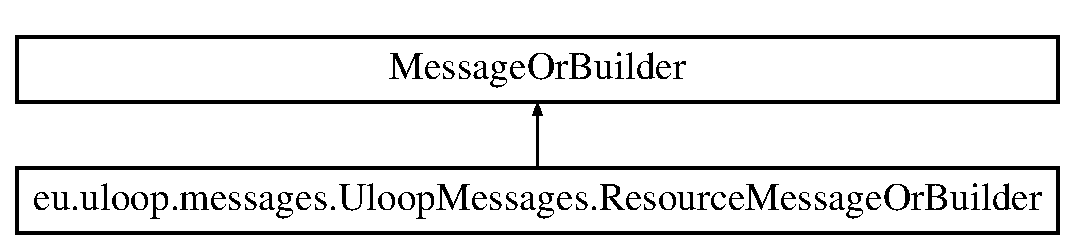
\includegraphics[height=2.000000cm]{interfaceeu_1_1uloop_1_1messages_1_1UloopMessages_1_1ResourceMessageOrBuilder}
\end{center}
\end{figure}
\subsection*{Public Member Functions}
\begin{DoxyCompactItemize}
\item 
boolean \hyperlink{interfaceeu_1_1uloop_1_1messages_1_1UloopMessages_1_1ResourceMessageOrBuilder_a2db6751208d16916b531aabc1b58a862}{has\+Rreq} ()
\item 
eu.\+uloop.\+messages.\+Uloop\+Messages.\+Enough\+Resources\+Message\+Request \hyperlink{interfaceeu_1_1uloop_1_1messages_1_1UloopMessages_1_1ResourceMessageOrBuilder_ae98606d380e06b735a00e58231a0ada1}{get\+Rreq} ()
\item 
\hyperlink{interfaceeu_1_1uloop_1_1messages_1_1UloopMessages_1_1EnoughResourcesMessageRequestOrBuilder}{eu.\+uloop.\+messages.\+Uloop\+Messages.\+Enough\+Resources\+Message\+Request\+Or\+Builder} \hyperlink{interfaceeu_1_1uloop_1_1messages_1_1UloopMessages_1_1ResourceMessageOrBuilder_a97d8ceec6a05fe2f27423f9353a4f139}{get\+Rreq\+Or\+Builder} ()
\item 
boolean \hyperlink{interfaceeu_1_1uloop_1_1messages_1_1UloopMessages_1_1ResourceMessageOrBuilder_a199164d0bc96a084d7533f3f23b0de7c}{has\+Rep} ()
\item 
eu.\+uloop.\+messages.\+Uloop\+Messages.\+Enough\+Resources\+Message\+Reply \hyperlink{interfaceeu_1_1uloop_1_1messages_1_1UloopMessages_1_1ResourceMessageOrBuilder_a91adc1c3c2a12e776e226e086eec07db}{get\+Rep} ()
\item 
\hyperlink{interfaceeu_1_1uloop_1_1messages_1_1UloopMessages_1_1EnoughResourcesMessageReplyOrBuilder}{eu.\+uloop.\+messages.\+Uloop\+Messages.\+Enough\+Resources\+Message\+Reply\+Or\+Builder} \hyperlink{interfaceeu_1_1uloop_1_1messages_1_1UloopMessages_1_1ResourceMessageOrBuilder_a4c00d4a6933d4459c7070bd1f7abe28d}{get\+Rep\+Or\+Builder} ()
\item 
boolean \hyperlink{interfaceeu_1_1uloop_1_1messages_1_1UloopMessages_1_1ResourceMessageOrBuilder_ae7499641905a50d2d77e69c6ca85e931}{has\+Cac} ()
\item 
eu.\+uloop.\+messages.\+Uloop\+Messages.\+Enough\+Resources\+C\+A\+C\+Reply \hyperlink{interfaceeu_1_1uloop_1_1messages_1_1UloopMessages_1_1ResourceMessageOrBuilder_af4b612edd0969178c242bde2959d55b3}{get\+Cac} ()
\item 
\hyperlink{interfaceeu_1_1uloop_1_1messages_1_1UloopMessages_1_1EnoughResourcesCACReplyOrBuilder}{eu.\+uloop.\+messages.\+Uloop\+Messages.\+Enough\+Resources\+C\+A\+C\+Reply\+Or\+Builder} \hyperlink{interfaceeu_1_1uloop_1_1messages_1_1UloopMessages_1_1ResourceMessageOrBuilder_ab847a44d1583afa22fe204054b24119c}{get\+Cac\+Or\+Builder} ()
\end{DoxyCompactItemize}


\subsection{Member Function Documentation}
\hypertarget{interfaceeu_1_1uloop_1_1messages_1_1UloopMessages_1_1ResourceMessageOrBuilder_af4b612edd0969178c242bde2959d55b3}{\index{eu\+::uloop\+::messages\+::\+Uloop\+Messages\+::\+Resource\+Message\+Or\+Builder@{eu\+::uloop\+::messages\+::\+Uloop\+Messages\+::\+Resource\+Message\+Or\+Builder}!get\+Cac@{get\+Cac}}
\index{get\+Cac@{get\+Cac}!eu\+::uloop\+::messages\+::\+Uloop\+Messages\+::\+Resource\+Message\+Or\+Builder@{eu\+::uloop\+::messages\+::\+Uloop\+Messages\+::\+Resource\+Message\+Or\+Builder}}
\subsubsection[{get\+Cac}]{\setlength{\rightskip}{0pt plus 5cm}eu.\+uloop.\+messages.\+Uloop\+Messages.\+Enough\+Resources\+C\+A\+C\+Reply eu.\+uloop.\+messages.\+Uloop\+Messages.\+Resource\+Message\+Or\+Builder.\+get\+Cac (
\begin{DoxyParamCaption}
{}
\end{DoxyParamCaption}
)}}\label{interfaceeu_1_1uloop_1_1messages_1_1UloopMessages_1_1ResourceMessageOrBuilder_af4b612edd0969178c242bde2959d55b3}
\hypertarget{interfaceeu_1_1uloop_1_1messages_1_1UloopMessages_1_1ResourceMessageOrBuilder_ab847a44d1583afa22fe204054b24119c}{\index{eu\+::uloop\+::messages\+::\+Uloop\+Messages\+::\+Resource\+Message\+Or\+Builder@{eu\+::uloop\+::messages\+::\+Uloop\+Messages\+::\+Resource\+Message\+Or\+Builder}!get\+Cac\+Or\+Builder@{get\+Cac\+Or\+Builder}}
\index{get\+Cac\+Or\+Builder@{get\+Cac\+Or\+Builder}!eu\+::uloop\+::messages\+::\+Uloop\+Messages\+::\+Resource\+Message\+Or\+Builder@{eu\+::uloop\+::messages\+::\+Uloop\+Messages\+::\+Resource\+Message\+Or\+Builder}}
\subsubsection[{get\+Cac\+Or\+Builder}]{\setlength{\rightskip}{0pt plus 5cm}{\bf eu.\+uloop.\+messages.\+Uloop\+Messages.\+Enough\+Resources\+C\+A\+C\+Reply\+Or\+Builder} eu.\+uloop.\+messages.\+Uloop\+Messages.\+Resource\+Message\+Or\+Builder.\+get\+Cac\+Or\+Builder (
\begin{DoxyParamCaption}
{}
\end{DoxyParamCaption}
)}}\label{interfaceeu_1_1uloop_1_1messages_1_1UloopMessages_1_1ResourceMessageOrBuilder_ab847a44d1583afa22fe204054b24119c}
\hypertarget{interfaceeu_1_1uloop_1_1messages_1_1UloopMessages_1_1ResourceMessageOrBuilder_a91adc1c3c2a12e776e226e086eec07db}{\index{eu\+::uloop\+::messages\+::\+Uloop\+Messages\+::\+Resource\+Message\+Or\+Builder@{eu\+::uloop\+::messages\+::\+Uloop\+Messages\+::\+Resource\+Message\+Or\+Builder}!get\+Rep@{get\+Rep}}
\index{get\+Rep@{get\+Rep}!eu\+::uloop\+::messages\+::\+Uloop\+Messages\+::\+Resource\+Message\+Or\+Builder@{eu\+::uloop\+::messages\+::\+Uloop\+Messages\+::\+Resource\+Message\+Or\+Builder}}
\subsubsection[{get\+Rep}]{\setlength{\rightskip}{0pt plus 5cm}eu.\+uloop.\+messages.\+Uloop\+Messages.\+Enough\+Resources\+Message\+Reply eu.\+uloop.\+messages.\+Uloop\+Messages.\+Resource\+Message\+Or\+Builder.\+get\+Rep (
\begin{DoxyParamCaption}
{}
\end{DoxyParamCaption}
)}}\label{interfaceeu_1_1uloop_1_1messages_1_1UloopMessages_1_1ResourceMessageOrBuilder_a91adc1c3c2a12e776e226e086eec07db}
\hypertarget{interfaceeu_1_1uloop_1_1messages_1_1UloopMessages_1_1ResourceMessageOrBuilder_a4c00d4a6933d4459c7070bd1f7abe28d}{\index{eu\+::uloop\+::messages\+::\+Uloop\+Messages\+::\+Resource\+Message\+Or\+Builder@{eu\+::uloop\+::messages\+::\+Uloop\+Messages\+::\+Resource\+Message\+Or\+Builder}!get\+Rep\+Or\+Builder@{get\+Rep\+Or\+Builder}}
\index{get\+Rep\+Or\+Builder@{get\+Rep\+Or\+Builder}!eu\+::uloop\+::messages\+::\+Uloop\+Messages\+::\+Resource\+Message\+Or\+Builder@{eu\+::uloop\+::messages\+::\+Uloop\+Messages\+::\+Resource\+Message\+Or\+Builder}}
\subsubsection[{get\+Rep\+Or\+Builder}]{\setlength{\rightskip}{0pt plus 5cm}{\bf eu.\+uloop.\+messages.\+Uloop\+Messages.\+Enough\+Resources\+Message\+Reply\+Or\+Builder} eu.\+uloop.\+messages.\+Uloop\+Messages.\+Resource\+Message\+Or\+Builder.\+get\+Rep\+Or\+Builder (
\begin{DoxyParamCaption}
{}
\end{DoxyParamCaption}
)}}\label{interfaceeu_1_1uloop_1_1messages_1_1UloopMessages_1_1ResourceMessageOrBuilder_a4c00d4a6933d4459c7070bd1f7abe28d}
\hypertarget{interfaceeu_1_1uloop_1_1messages_1_1UloopMessages_1_1ResourceMessageOrBuilder_ae98606d380e06b735a00e58231a0ada1}{\index{eu\+::uloop\+::messages\+::\+Uloop\+Messages\+::\+Resource\+Message\+Or\+Builder@{eu\+::uloop\+::messages\+::\+Uloop\+Messages\+::\+Resource\+Message\+Or\+Builder}!get\+Rreq@{get\+Rreq}}
\index{get\+Rreq@{get\+Rreq}!eu\+::uloop\+::messages\+::\+Uloop\+Messages\+::\+Resource\+Message\+Or\+Builder@{eu\+::uloop\+::messages\+::\+Uloop\+Messages\+::\+Resource\+Message\+Or\+Builder}}
\subsubsection[{get\+Rreq}]{\setlength{\rightskip}{0pt plus 5cm}eu.\+uloop.\+messages.\+Uloop\+Messages.\+Enough\+Resources\+Message\+Request eu.\+uloop.\+messages.\+Uloop\+Messages.\+Resource\+Message\+Or\+Builder.\+get\+Rreq (
\begin{DoxyParamCaption}
{}
\end{DoxyParamCaption}
)}}\label{interfaceeu_1_1uloop_1_1messages_1_1UloopMessages_1_1ResourceMessageOrBuilder_ae98606d380e06b735a00e58231a0ada1}
\hypertarget{interfaceeu_1_1uloop_1_1messages_1_1UloopMessages_1_1ResourceMessageOrBuilder_a97d8ceec6a05fe2f27423f9353a4f139}{\index{eu\+::uloop\+::messages\+::\+Uloop\+Messages\+::\+Resource\+Message\+Or\+Builder@{eu\+::uloop\+::messages\+::\+Uloop\+Messages\+::\+Resource\+Message\+Or\+Builder}!get\+Rreq\+Or\+Builder@{get\+Rreq\+Or\+Builder}}
\index{get\+Rreq\+Or\+Builder@{get\+Rreq\+Or\+Builder}!eu\+::uloop\+::messages\+::\+Uloop\+Messages\+::\+Resource\+Message\+Or\+Builder@{eu\+::uloop\+::messages\+::\+Uloop\+Messages\+::\+Resource\+Message\+Or\+Builder}}
\subsubsection[{get\+Rreq\+Or\+Builder}]{\setlength{\rightskip}{0pt plus 5cm}{\bf eu.\+uloop.\+messages.\+Uloop\+Messages.\+Enough\+Resources\+Message\+Request\+Or\+Builder} eu.\+uloop.\+messages.\+Uloop\+Messages.\+Resource\+Message\+Or\+Builder.\+get\+Rreq\+Or\+Builder (
\begin{DoxyParamCaption}
{}
\end{DoxyParamCaption}
)}}\label{interfaceeu_1_1uloop_1_1messages_1_1UloopMessages_1_1ResourceMessageOrBuilder_a97d8ceec6a05fe2f27423f9353a4f139}
\hypertarget{interfaceeu_1_1uloop_1_1messages_1_1UloopMessages_1_1ResourceMessageOrBuilder_ae7499641905a50d2d77e69c6ca85e931}{\index{eu\+::uloop\+::messages\+::\+Uloop\+Messages\+::\+Resource\+Message\+Or\+Builder@{eu\+::uloop\+::messages\+::\+Uloop\+Messages\+::\+Resource\+Message\+Or\+Builder}!has\+Cac@{has\+Cac}}
\index{has\+Cac@{has\+Cac}!eu\+::uloop\+::messages\+::\+Uloop\+Messages\+::\+Resource\+Message\+Or\+Builder@{eu\+::uloop\+::messages\+::\+Uloop\+Messages\+::\+Resource\+Message\+Or\+Builder}}
\subsubsection[{has\+Cac}]{\setlength{\rightskip}{0pt plus 5cm}boolean eu.\+uloop.\+messages.\+Uloop\+Messages.\+Resource\+Message\+Or\+Builder.\+has\+Cac (
\begin{DoxyParamCaption}
{}
\end{DoxyParamCaption}
)}}\label{interfaceeu_1_1uloop_1_1messages_1_1UloopMessages_1_1ResourceMessageOrBuilder_ae7499641905a50d2d77e69c6ca85e931}
\hypertarget{interfaceeu_1_1uloop_1_1messages_1_1UloopMessages_1_1ResourceMessageOrBuilder_a199164d0bc96a084d7533f3f23b0de7c}{\index{eu\+::uloop\+::messages\+::\+Uloop\+Messages\+::\+Resource\+Message\+Or\+Builder@{eu\+::uloop\+::messages\+::\+Uloop\+Messages\+::\+Resource\+Message\+Or\+Builder}!has\+Rep@{has\+Rep}}
\index{has\+Rep@{has\+Rep}!eu\+::uloop\+::messages\+::\+Uloop\+Messages\+::\+Resource\+Message\+Or\+Builder@{eu\+::uloop\+::messages\+::\+Uloop\+Messages\+::\+Resource\+Message\+Or\+Builder}}
\subsubsection[{has\+Rep}]{\setlength{\rightskip}{0pt plus 5cm}boolean eu.\+uloop.\+messages.\+Uloop\+Messages.\+Resource\+Message\+Or\+Builder.\+has\+Rep (
\begin{DoxyParamCaption}
{}
\end{DoxyParamCaption}
)}}\label{interfaceeu_1_1uloop_1_1messages_1_1UloopMessages_1_1ResourceMessageOrBuilder_a199164d0bc96a084d7533f3f23b0de7c}
\hypertarget{interfaceeu_1_1uloop_1_1messages_1_1UloopMessages_1_1ResourceMessageOrBuilder_a2db6751208d16916b531aabc1b58a862}{\index{eu\+::uloop\+::messages\+::\+Uloop\+Messages\+::\+Resource\+Message\+Or\+Builder@{eu\+::uloop\+::messages\+::\+Uloop\+Messages\+::\+Resource\+Message\+Or\+Builder}!has\+Rreq@{has\+Rreq}}
\index{has\+Rreq@{has\+Rreq}!eu\+::uloop\+::messages\+::\+Uloop\+Messages\+::\+Resource\+Message\+Or\+Builder@{eu\+::uloop\+::messages\+::\+Uloop\+Messages\+::\+Resource\+Message\+Or\+Builder}}
\subsubsection[{has\+Rreq}]{\setlength{\rightskip}{0pt plus 5cm}boolean eu.\+uloop.\+messages.\+Uloop\+Messages.\+Resource\+Message\+Or\+Builder.\+has\+Rreq (
\begin{DoxyParamCaption}
{}
\end{DoxyParamCaption}
)}}\label{interfaceeu_1_1uloop_1_1messages_1_1UloopMessages_1_1ResourceMessageOrBuilder_a2db6751208d16916b531aabc1b58a862}


The documentation for this interface was generated from the following file\+:\begin{DoxyCompactItemize}
\item 
src/eu/uloop/messages/\hyperlink{UloopMessages_8java}{Uloop\+Messages.\+java}\end{DoxyCompactItemize}

\hypertarget{classeu_1_1uloop_1_1mobilitytracker_1_1MTrackerService_1_1SendInformationWithGatewayTask}{\section{eu.\+uloop.\+mobilitytracker.\+M\+Tracker\+Service.\+Send\+Information\+With\+Gateway\+Task Class Reference}
\label{classeu_1_1uloop_1_1mobilitytracker_1_1MTrackerService_1_1SendInformationWithGatewayTask}\index{eu.\+uloop.\+mobilitytracker.\+M\+Tracker\+Service.\+Send\+Information\+With\+Gateway\+Task@{eu.\+uloop.\+mobilitytracker.\+M\+Tracker\+Service.\+Send\+Information\+With\+Gateway\+Task}}
}
Inheritance diagram for eu.\+uloop.\+mobilitytracker.\+M\+Tracker\+Service.\+Send\+Information\+With\+Gateway\+Task\+:\begin{figure}[H]
\begin{center}
\leavevmode
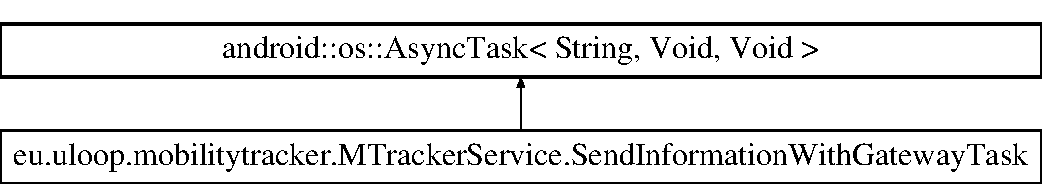
\includegraphics[height=2.000000cm]{classeu_1_1uloop_1_1mobilitytracker_1_1MTrackerService_1_1SendInformationWithGatewayTask}
\end{center}
\end{figure}
\subsection*{Protected Member Functions}
\begin{DoxyCompactItemize}
\item 
Void \hyperlink{classeu_1_1uloop_1_1mobilitytracker_1_1MTrackerService_1_1SendInformationWithGatewayTask_adbcf100edb442c27fc18e44bce9bb66d}{do\+In\+Background} (String...\+parameters)
\end{DoxyCompactItemize}


\subsection{Member Function Documentation}
\hypertarget{classeu_1_1uloop_1_1mobilitytracker_1_1MTrackerService_1_1SendInformationWithGatewayTask_adbcf100edb442c27fc18e44bce9bb66d}{\index{eu\+::uloop\+::mobilitytracker\+::\+M\+Tracker\+Service\+::\+Send\+Information\+With\+Gateway\+Task@{eu\+::uloop\+::mobilitytracker\+::\+M\+Tracker\+Service\+::\+Send\+Information\+With\+Gateway\+Task}!do\+In\+Background@{do\+In\+Background}}
\index{do\+In\+Background@{do\+In\+Background}!eu\+::uloop\+::mobilitytracker\+::\+M\+Tracker\+Service\+::\+Send\+Information\+With\+Gateway\+Task@{eu\+::uloop\+::mobilitytracker\+::\+M\+Tracker\+Service\+::\+Send\+Information\+With\+Gateway\+Task}}
\subsubsection[{do\+In\+Background}]{\setlength{\rightskip}{0pt plus 5cm}Void eu.\+uloop.\+mobilitytracker.\+M\+Tracker\+Service.\+Send\+Information\+With\+Gateway\+Task.\+do\+In\+Background (
\begin{DoxyParamCaption}
\item[{String...}]{parameters}
\end{DoxyParamCaption}
)\hspace{0.3cm}{\ttfamily [protected]}}}\label{classeu_1_1uloop_1_1mobilitytracker_1_1MTrackerService_1_1SendInformationWithGatewayTask_adbcf100edb442c27fc18e44bce9bb66d}


The documentation for this class was generated from the following file\+:\begin{DoxyCompactItemize}
\item 
src/eu/uloop/mobilitytracker/\hyperlink{MTrackerService_8java}{M\+Tracker\+Service.\+java}\end{DoxyCompactItemize}

\hypertarget{interfaceeu_1_1uloop_1_1messages_1_1UloopMessages_1_1ServiceMessageOrBuilder}{\section{eu.\+uloop.\+messages.\+Uloop\+Messages.\+Service\+Message\+Or\+Builder Interface Reference}
\label{interfaceeu_1_1uloop_1_1messages_1_1UloopMessages_1_1ServiceMessageOrBuilder}\index{eu.\+uloop.\+messages.\+Uloop\+Messages.\+Service\+Message\+Or\+Builder@{eu.\+uloop.\+messages.\+Uloop\+Messages.\+Service\+Message\+Or\+Builder}}
}
Inheritance diagram for eu.\+uloop.\+messages.\+Uloop\+Messages.\+Service\+Message\+Or\+Builder\+:\begin{figure}[H]
\begin{center}
\leavevmode
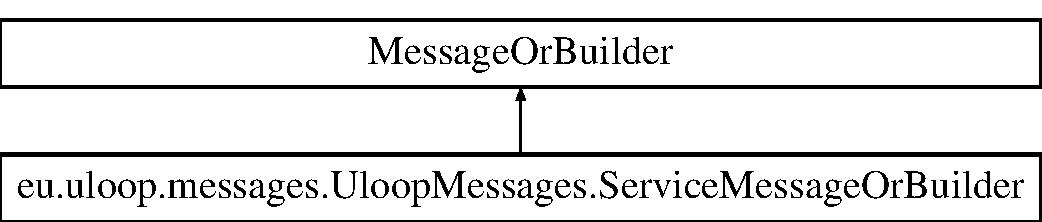
\includegraphics[height=2.000000cm]{interfaceeu_1_1uloop_1_1messages_1_1UloopMessages_1_1ServiceMessageOrBuilder}
\end{center}
\end{figure}
\subsection*{Public Member Functions}
\begin{DoxyCompactItemize}
\item 
boolean \hyperlink{interfaceeu_1_1uloop_1_1messages_1_1UloopMessages_1_1ServiceMessageOrBuilder_a1952f45ff7946db29a62a20dc5267cdb}{has\+Servreq} ()
\item 
eu.\+uloop.\+messages.\+Uloop\+Messages.\+Service\+Request \hyperlink{interfaceeu_1_1uloop_1_1messages_1_1UloopMessages_1_1ServiceMessageOrBuilder_ab86bf09d976574b2128e93073e626fba}{get\+Servreq} ()
\item 
\hyperlink{interfaceeu_1_1uloop_1_1messages_1_1UloopMessages_1_1ServiceRequestOrBuilder}{eu.\+uloop.\+messages.\+Uloop\+Messages.\+Service\+Request\+Or\+Builder} \hyperlink{interfaceeu_1_1uloop_1_1messages_1_1UloopMessages_1_1ServiceMessageOrBuilder_a46f4131ed0a7585241c571810be138ff}{get\+Servreq\+Or\+Builder} ()
\item 
boolean \hyperlink{interfaceeu_1_1uloop_1_1messages_1_1UloopMessages_1_1ServiceMessageOrBuilder_affb470e750c7ef23d54afe022a1bd29b}{has\+Servrep} ()
\item 
eu.\+uloop.\+messages.\+Uloop\+Messages.\+Service\+Reply \hyperlink{interfaceeu_1_1uloop_1_1messages_1_1UloopMessages_1_1ServiceMessageOrBuilder_ac7ff577bd5912e9d40fc0c18d37a3deb}{get\+Servrep} ()
\item 
\hyperlink{interfaceeu_1_1uloop_1_1messages_1_1UloopMessages_1_1ServiceReplyOrBuilder}{eu.\+uloop.\+messages.\+Uloop\+Messages.\+Service\+Reply\+Or\+Builder} \hyperlink{interfaceeu_1_1uloop_1_1messages_1_1UloopMessages_1_1ServiceMessageOrBuilder_a3aae6e0bec0a30fa6c06fd5851eae04b}{get\+Servrep\+Or\+Builder} ()
\item 
boolean \hyperlink{interfaceeu_1_1uloop_1_1messages_1_1UloopMessages_1_1ServiceMessageOrBuilder_ac6a414247d4280f51d456efb7c12534d}{has\+Servup} ()
\item 
eu.\+uloop.\+messages.\+Uloop\+Messages.\+Service\+Update \hyperlink{interfaceeu_1_1uloop_1_1messages_1_1UloopMessages_1_1ServiceMessageOrBuilder_a713d42f22f254989ca00efcbdef04cfe}{get\+Servup} ()
\item 
\hyperlink{interfaceeu_1_1uloop_1_1messages_1_1UloopMessages_1_1ServiceUpdateOrBuilder}{eu.\+uloop.\+messages.\+Uloop\+Messages.\+Service\+Update\+Or\+Builder} \hyperlink{interfaceeu_1_1uloop_1_1messages_1_1UloopMessages_1_1ServiceMessageOrBuilder_a0b6172369b6877924b1fb8be0b730b7b}{get\+Servup\+Or\+Builder} ()
\end{DoxyCompactItemize}


\subsection{Member Function Documentation}
\hypertarget{interfaceeu_1_1uloop_1_1messages_1_1UloopMessages_1_1ServiceMessageOrBuilder_ac7ff577bd5912e9d40fc0c18d37a3deb}{\index{eu\+::uloop\+::messages\+::\+Uloop\+Messages\+::\+Service\+Message\+Or\+Builder@{eu\+::uloop\+::messages\+::\+Uloop\+Messages\+::\+Service\+Message\+Or\+Builder}!get\+Servrep@{get\+Servrep}}
\index{get\+Servrep@{get\+Servrep}!eu\+::uloop\+::messages\+::\+Uloop\+Messages\+::\+Service\+Message\+Or\+Builder@{eu\+::uloop\+::messages\+::\+Uloop\+Messages\+::\+Service\+Message\+Or\+Builder}}
\subsubsection[{get\+Servrep}]{\setlength{\rightskip}{0pt plus 5cm}eu.\+uloop.\+messages.\+Uloop\+Messages.\+Service\+Reply eu.\+uloop.\+messages.\+Uloop\+Messages.\+Service\+Message\+Or\+Builder.\+get\+Servrep (
\begin{DoxyParamCaption}
{}
\end{DoxyParamCaption}
)}}\label{interfaceeu_1_1uloop_1_1messages_1_1UloopMessages_1_1ServiceMessageOrBuilder_ac7ff577bd5912e9d40fc0c18d37a3deb}
\hypertarget{interfaceeu_1_1uloop_1_1messages_1_1UloopMessages_1_1ServiceMessageOrBuilder_a3aae6e0bec0a30fa6c06fd5851eae04b}{\index{eu\+::uloop\+::messages\+::\+Uloop\+Messages\+::\+Service\+Message\+Or\+Builder@{eu\+::uloop\+::messages\+::\+Uloop\+Messages\+::\+Service\+Message\+Or\+Builder}!get\+Servrep\+Or\+Builder@{get\+Servrep\+Or\+Builder}}
\index{get\+Servrep\+Or\+Builder@{get\+Servrep\+Or\+Builder}!eu\+::uloop\+::messages\+::\+Uloop\+Messages\+::\+Service\+Message\+Or\+Builder@{eu\+::uloop\+::messages\+::\+Uloop\+Messages\+::\+Service\+Message\+Or\+Builder}}
\subsubsection[{get\+Servrep\+Or\+Builder}]{\setlength{\rightskip}{0pt plus 5cm}{\bf eu.\+uloop.\+messages.\+Uloop\+Messages.\+Service\+Reply\+Or\+Builder} eu.\+uloop.\+messages.\+Uloop\+Messages.\+Service\+Message\+Or\+Builder.\+get\+Servrep\+Or\+Builder (
\begin{DoxyParamCaption}
{}
\end{DoxyParamCaption}
)}}\label{interfaceeu_1_1uloop_1_1messages_1_1UloopMessages_1_1ServiceMessageOrBuilder_a3aae6e0bec0a30fa6c06fd5851eae04b}
\hypertarget{interfaceeu_1_1uloop_1_1messages_1_1UloopMessages_1_1ServiceMessageOrBuilder_ab86bf09d976574b2128e93073e626fba}{\index{eu\+::uloop\+::messages\+::\+Uloop\+Messages\+::\+Service\+Message\+Or\+Builder@{eu\+::uloop\+::messages\+::\+Uloop\+Messages\+::\+Service\+Message\+Or\+Builder}!get\+Servreq@{get\+Servreq}}
\index{get\+Servreq@{get\+Servreq}!eu\+::uloop\+::messages\+::\+Uloop\+Messages\+::\+Service\+Message\+Or\+Builder@{eu\+::uloop\+::messages\+::\+Uloop\+Messages\+::\+Service\+Message\+Or\+Builder}}
\subsubsection[{get\+Servreq}]{\setlength{\rightskip}{0pt plus 5cm}eu.\+uloop.\+messages.\+Uloop\+Messages.\+Service\+Request eu.\+uloop.\+messages.\+Uloop\+Messages.\+Service\+Message\+Or\+Builder.\+get\+Servreq (
\begin{DoxyParamCaption}
{}
\end{DoxyParamCaption}
)}}\label{interfaceeu_1_1uloop_1_1messages_1_1UloopMessages_1_1ServiceMessageOrBuilder_ab86bf09d976574b2128e93073e626fba}
\hypertarget{interfaceeu_1_1uloop_1_1messages_1_1UloopMessages_1_1ServiceMessageOrBuilder_a46f4131ed0a7585241c571810be138ff}{\index{eu\+::uloop\+::messages\+::\+Uloop\+Messages\+::\+Service\+Message\+Or\+Builder@{eu\+::uloop\+::messages\+::\+Uloop\+Messages\+::\+Service\+Message\+Or\+Builder}!get\+Servreq\+Or\+Builder@{get\+Servreq\+Or\+Builder}}
\index{get\+Servreq\+Or\+Builder@{get\+Servreq\+Or\+Builder}!eu\+::uloop\+::messages\+::\+Uloop\+Messages\+::\+Service\+Message\+Or\+Builder@{eu\+::uloop\+::messages\+::\+Uloop\+Messages\+::\+Service\+Message\+Or\+Builder}}
\subsubsection[{get\+Servreq\+Or\+Builder}]{\setlength{\rightskip}{0pt plus 5cm}{\bf eu.\+uloop.\+messages.\+Uloop\+Messages.\+Service\+Request\+Or\+Builder} eu.\+uloop.\+messages.\+Uloop\+Messages.\+Service\+Message\+Or\+Builder.\+get\+Servreq\+Or\+Builder (
\begin{DoxyParamCaption}
{}
\end{DoxyParamCaption}
)}}\label{interfaceeu_1_1uloop_1_1messages_1_1UloopMessages_1_1ServiceMessageOrBuilder_a46f4131ed0a7585241c571810be138ff}
\hypertarget{interfaceeu_1_1uloop_1_1messages_1_1UloopMessages_1_1ServiceMessageOrBuilder_a713d42f22f254989ca00efcbdef04cfe}{\index{eu\+::uloop\+::messages\+::\+Uloop\+Messages\+::\+Service\+Message\+Or\+Builder@{eu\+::uloop\+::messages\+::\+Uloop\+Messages\+::\+Service\+Message\+Or\+Builder}!get\+Servup@{get\+Servup}}
\index{get\+Servup@{get\+Servup}!eu\+::uloop\+::messages\+::\+Uloop\+Messages\+::\+Service\+Message\+Or\+Builder@{eu\+::uloop\+::messages\+::\+Uloop\+Messages\+::\+Service\+Message\+Or\+Builder}}
\subsubsection[{get\+Servup}]{\setlength{\rightskip}{0pt plus 5cm}eu.\+uloop.\+messages.\+Uloop\+Messages.\+Service\+Update eu.\+uloop.\+messages.\+Uloop\+Messages.\+Service\+Message\+Or\+Builder.\+get\+Servup (
\begin{DoxyParamCaption}
{}
\end{DoxyParamCaption}
)}}\label{interfaceeu_1_1uloop_1_1messages_1_1UloopMessages_1_1ServiceMessageOrBuilder_a713d42f22f254989ca00efcbdef04cfe}
\hypertarget{interfaceeu_1_1uloop_1_1messages_1_1UloopMessages_1_1ServiceMessageOrBuilder_a0b6172369b6877924b1fb8be0b730b7b}{\index{eu\+::uloop\+::messages\+::\+Uloop\+Messages\+::\+Service\+Message\+Or\+Builder@{eu\+::uloop\+::messages\+::\+Uloop\+Messages\+::\+Service\+Message\+Or\+Builder}!get\+Servup\+Or\+Builder@{get\+Servup\+Or\+Builder}}
\index{get\+Servup\+Or\+Builder@{get\+Servup\+Or\+Builder}!eu\+::uloop\+::messages\+::\+Uloop\+Messages\+::\+Service\+Message\+Or\+Builder@{eu\+::uloop\+::messages\+::\+Uloop\+Messages\+::\+Service\+Message\+Or\+Builder}}
\subsubsection[{get\+Servup\+Or\+Builder}]{\setlength{\rightskip}{0pt plus 5cm}{\bf eu.\+uloop.\+messages.\+Uloop\+Messages.\+Service\+Update\+Or\+Builder} eu.\+uloop.\+messages.\+Uloop\+Messages.\+Service\+Message\+Or\+Builder.\+get\+Servup\+Or\+Builder (
\begin{DoxyParamCaption}
{}
\end{DoxyParamCaption}
)}}\label{interfaceeu_1_1uloop_1_1messages_1_1UloopMessages_1_1ServiceMessageOrBuilder_a0b6172369b6877924b1fb8be0b730b7b}
\hypertarget{interfaceeu_1_1uloop_1_1messages_1_1UloopMessages_1_1ServiceMessageOrBuilder_affb470e750c7ef23d54afe022a1bd29b}{\index{eu\+::uloop\+::messages\+::\+Uloop\+Messages\+::\+Service\+Message\+Or\+Builder@{eu\+::uloop\+::messages\+::\+Uloop\+Messages\+::\+Service\+Message\+Or\+Builder}!has\+Servrep@{has\+Servrep}}
\index{has\+Servrep@{has\+Servrep}!eu\+::uloop\+::messages\+::\+Uloop\+Messages\+::\+Service\+Message\+Or\+Builder@{eu\+::uloop\+::messages\+::\+Uloop\+Messages\+::\+Service\+Message\+Or\+Builder}}
\subsubsection[{has\+Servrep}]{\setlength{\rightskip}{0pt plus 5cm}boolean eu.\+uloop.\+messages.\+Uloop\+Messages.\+Service\+Message\+Or\+Builder.\+has\+Servrep (
\begin{DoxyParamCaption}
{}
\end{DoxyParamCaption}
)}}\label{interfaceeu_1_1uloop_1_1messages_1_1UloopMessages_1_1ServiceMessageOrBuilder_affb470e750c7ef23d54afe022a1bd29b}
\hypertarget{interfaceeu_1_1uloop_1_1messages_1_1UloopMessages_1_1ServiceMessageOrBuilder_a1952f45ff7946db29a62a20dc5267cdb}{\index{eu\+::uloop\+::messages\+::\+Uloop\+Messages\+::\+Service\+Message\+Or\+Builder@{eu\+::uloop\+::messages\+::\+Uloop\+Messages\+::\+Service\+Message\+Or\+Builder}!has\+Servreq@{has\+Servreq}}
\index{has\+Servreq@{has\+Servreq}!eu\+::uloop\+::messages\+::\+Uloop\+Messages\+::\+Service\+Message\+Or\+Builder@{eu\+::uloop\+::messages\+::\+Uloop\+Messages\+::\+Service\+Message\+Or\+Builder}}
\subsubsection[{has\+Servreq}]{\setlength{\rightskip}{0pt plus 5cm}boolean eu.\+uloop.\+messages.\+Uloop\+Messages.\+Service\+Message\+Or\+Builder.\+has\+Servreq (
\begin{DoxyParamCaption}
{}
\end{DoxyParamCaption}
)}}\label{interfaceeu_1_1uloop_1_1messages_1_1UloopMessages_1_1ServiceMessageOrBuilder_a1952f45ff7946db29a62a20dc5267cdb}
\hypertarget{interfaceeu_1_1uloop_1_1messages_1_1UloopMessages_1_1ServiceMessageOrBuilder_ac6a414247d4280f51d456efb7c12534d}{\index{eu\+::uloop\+::messages\+::\+Uloop\+Messages\+::\+Service\+Message\+Or\+Builder@{eu\+::uloop\+::messages\+::\+Uloop\+Messages\+::\+Service\+Message\+Or\+Builder}!has\+Servup@{has\+Servup}}
\index{has\+Servup@{has\+Servup}!eu\+::uloop\+::messages\+::\+Uloop\+Messages\+::\+Service\+Message\+Or\+Builder@{eu\+::uloop\+::messages\+::\+Uloop\+Messages\+::\+Service\+Message\+Or\+Builder}}
\subsubsection[{has\+Servup}]{\setlength{\rightskip}{0pt plus 5cm}boolean eu.\+uloop.\+messages.\+Uloop\+Messages.\+Service\+Message\+Or\+Builder.\+has\+Servup (
\begin{DoxyParamCaption}
{}
\end{DoxyParamCaption}
)}}\label{interfaceeu_1_1uloop_1_1messages_1_1UloopMessages_1_1ServiceMessageOrBuilder_ac6a414247d4280f51d456efb7c12534d}


The documentation for this interface was generated from the following file\+:\begin{DoxyCompactItemize}
\item 
src/eu/uloop/messages/\hyperlink{UloopMessages_8java}{Uloop\+Messages.\+java}\end{DoxyCompactItemize}

\hypertarget{interfaceeu_1_1uloop_1_1messages_1_1UloopMessages_1_1ServiceReplyOrBuilder}{\section{eu.\+uloop.\+messages.\+Uloop\+Messages.\+Service\+Reply\+Or\+Builder Interface Reference}
\label{interfaceeu_1_1uloop_1_1messages_1_1UloopMessages_1_1ServiceReplyOrBuilder}\index{eu.\+uloop.\+messages.\+Uloop\+Messages.\+Service\+Reply\+Or\+Builder@{eu.\+uloop.\+messages.\+Uloop\+Messages.\+Service\+Reply\+Or\+Builder}}
}
Inheritance diagram for eu.\+uloop.\+messages.\+Uloop\+Messages.\+Service\+Reply\+Or\+Builder\+:\begin{figure}[H]
\begin{center}
\leavevmode
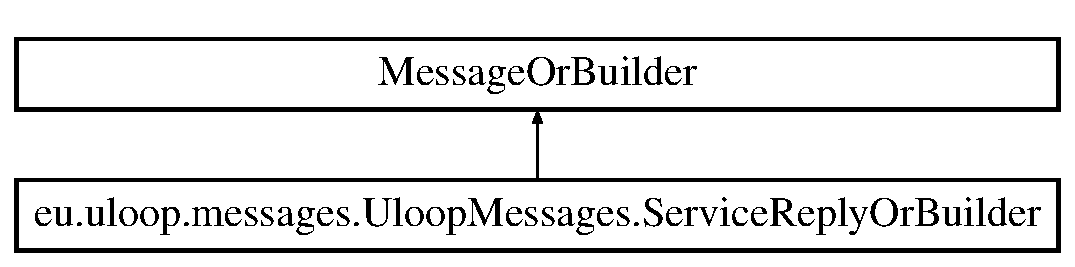
\includegraphics[height=2.000000cm]{interfaceeu_1_1uloop_1_1messages_1_1UloopMessages_1_1ServiceReplyOrBuilder}
\end{center}
\end{figure}
\subsection*{Public Member Functions}
\begin{DoxyCompactItemize}
\item 
boolean \hyperlink{interfaceeu_1_1uloop_1_1messages_1_1UloopMessages_1_1ServiceReplyOrBuilder_a00a63d749b092eae1bab0c3c3bf2dcce}{has\+Cryptoid} ()
\item 
com.\+google.\+protobuf.\+Byte\+String \hyperlink{interfaceeu_1_1uloop_1_1messages_1_1UloopMessages_1_1ServiceReplyOrBuilder_a720498654fe93facff572da81cf11b8b}{get\+Cryptoid} ()
\item 
boolean \hyperlink{interfaceeu_1_1uloop_1_1messages_1_1UloopMessages_1_1ServiceReplyOrBuilder_abe924eaca1952c00536fe5d0032dc0a7}{has\+Trust} ()
\item 
double \hyperlink{interfaceeu_1_1uloop_1_1messages_1_1UloopMessages_1_1ServiceReplyOrBuilder_a330d600e46cf197c578dc5bc9b845ba8}{get\+Trust} ()
\item 
boolean \hyperlink{interfaceeu_1_1uloop_1_1messages_1_1UloopMessages_1_1ServiceReplyOrBuilder_ac536738a1e28c718131e24e0f5136723}{has\+Authorization} ()
\item 
boolean \hyperlink{interfaceeu_1_1uloop_1_1messages_1_1UloopMessages_1_1ServiceReplyOrBuilder_ad63f56423b7f94d0efd4e06bd3652180}{get\+Authorization} ()
\end{DoxyCompactItemize}


\subsection{Member Function Documentation}
\hypertarget{interfaceeu_1_1uloop_1_1messages_1_1UloopMessages_1_1ServiceReplyOrBuilder_ad63f56423b7f94d0efd4e06bd3652180}{\index{eu\+::uloop\+::messages\+::\+Uloop\+Messages\+::\+Service\+Reply\+Or\+Builder@{eu\+::uloop\+::messages\+::\+Uloop\+Messages\+::\+Service\+Reply\+Or\+Builder}!get\+Authorization@{get\+Authorization}}
\index{get\+Authorization@{get\+Authorization}!eu\+::uloop\+::messages\+::\+Uloop\+Messages\+::\+Service\+Reply\+Or\+Builder@{eu\+::uloop\+::messages\+::\+Uloop\+Messages\+::\+Service\+Reply\+Or\+Builder}}
\subsubsection[{get\+Authorization}]{\setlength{\rightskip}{0pt plus 5cm}boolean eu.\+uloop.\+messages.\+Uloop\+Messages.\+Service\+Reply\+Or\+Builder.\+get\+Authorization (
\begin{DoxyParamCaption}
{}
\end{DoxyParamCaption}
)}}\label{interfaceeu_1_1uloop_1_1messages_1_1UloopMessages_1_1ServiceReplyOrBuilder_ad63f56423b7f94d0efd4e06bd3652180}
\hypertarget{interfaceeu_1_1uloop_1_1messages_1_1UloopMessages_1_1ServiceReplyOrBuilder_a720498654fe93facff572da81cf11b8b}{\index{eu\+::uloop\+::messages\+::\+Uloop\+Messages\+::\+Service\+Reply\+Or\+Builder@{eu\+::uloop\+::messages\+::\+Uloop\+Messages\+::\+Service\+Reply\+Or\+Builder}!get\+Cryptoid@{get\+Cryptoid}}
\index{get\+Cryptoid@{get\+Cryptoid}!eu\+::uloop\+::messages\+::\+Uloop\+Messages\+::\+Service\+Reply\+Or\+Builder@{eu\+::uloop\+::messages\+::\+Uloop\+Messages\+::\+Service\+Reply\+Or\+Builder}}
\subsubsection[{get\+Cryptoid}]{\setlength{\rightskip}{0pt plus 5cm}com.\+google.\+protobuf.\+Byte\+String eu.\+uloop.\+messages.\+Uloop\+Messages.\+Service\+Reply\+Or\+Builder.\+get\+Cryptoid (
\begin{DoxyParamCaption}
{}
\end{DoxyParamCaption}
)}}\label{interfaceeu_1_1uloop_1_1messages_1_1UloopMessages_1_1ServiceReplyOrBuilder_a720498654fe93facff572da81cf11b8b}
\hypertarget{interfaceeu_1_1uloop_1_1messages_1_1UloopMessages_1_1ServiceReplyOrBuilder_a330d600e46cf197c578dc5bc9b845ba8}{\index{eu\+::uloop\+::messages\+::\+Uloop\+Messages\+::\+Service\+Reply\+Or\+Builder@{eu\+::uloop\+::messages\+::\+Uloop\+Messages\+::\+Service\+Reply\+Or\+Builder}!get\+Trust@{get\+Trust}}
\index{get\+Trust@{get\+Trust}!eu\+::uloop\+::messages\+::\+Uloop\+Messages\+::\+Service\+Reply\+Or\+Builder@{eu\+::uloop\+::messages\+::\+Uloop\+Messages\+::\+Service\+Reply\+Or\+Builder}}
\subsubsection[{get\+Trust}]{\setlength{\rightskip}{0pt plus 5cm}double eu.\+uloop.\+messages.\+Uloop\+Messages.\+Service\+Reply\+Or\+Builder.\+get\+Trust (
\begin{DoxyParamCaption}
{}
\end{DoxyParamCaption}
)}}\label{interfaceeu_1_1uloop_1_1messages_1_1UloopMessages_1_1ServiceReplyOrBuilder_a330d600e46cf197c578dc5bc9b845ba8}
\hypertarget{interfaceeu_1_1uloop_1_1messages_1_1UloopMessages_1_1ServiceReplyOrBuilder_ac536738a1e28c718131e24e0f5136723}{\index{eu\+::uloop\+::messages\+::\+Uloop\+Messages\+::\+Service\+Reply\+Or\+Builder@{eu\+::uloop\+::messages\+::\+Uloop\+Messages\+::\+Service\+Reply\+Or\+Builder}!has\+Authorization@{has\+Authorization}}
\index{has\+Authorization@{has\+Authorization}!eu\+::uloop\+::messages\+::\+Uloop\+Messages\+::\+Service\+Reply\+Or\+Builder@{eu\+::uloop\+::messages\+::\+Uloop\+Messages\+::\+Service\+Reply\+Or\+Builder}}
\subsubsection[{has\+Authorization}]{\setlength{\rightskip}{0pt plus 5cm}boolean eu.\+uloop.\+messages.\+Uloop\+Messages.\+Service\+Reply\+Or\+Builder.\+has\+Authorization (
\begin{DoxyParamCaption}
{}
\end{DoxyParamCaption}
)}}\label{interfaceeu_1_1uloop_1_1messages_1_1UloopMessages_1_1ServiceReplyOrBuilder_ac536738a1e28c718131e24e0f5136723}
\hypertarget{interfaceeu_1_1uloop_1_1messages_1_1UloopMessages_1_1ServiceReplyOrBuilder_a00a63d749b092eae1bab0c3c3bf2dcce}{\index{eu\+::uloop\+::messages\+::\+Uloop\+Messages\+::\+Service\+Reply\+Or\+Builder@{eu\+::uloop\+::messages\+::\+Uloop\+Messages\+::\+Service\+Reply\+Or\+Builder}!has\+Cryptoid@{has\+Cryptoid}}
\index{has\+Cryptoid@{has\+Cryptoid}!eu\+::uloop\+::messages\+::\+Uloop\+Messages\+::\+Service\+Reply\+Or\+Builder@{eu\+::uloop\+::messages\+::\+Uloop\+Messages\+::\+Service\+Reply\+Or\+Builder}}
\subsubsection[{has\+Cryptoid}]{\setlength{\rightskip}{0pt plus 5cm}boolean eu.\+uloop.\+messages.\+Uloop\+Messages.\+Service\+Reply\+Or\+Builder.\+has\+Cryptoid (
\begin{DoxyParamCaption}
{}
\end{DoxyParamCaption}
)}}\label{interfaceeu_1_1uloop_1_1messages_1_1UloopMessages_1_1ServiceReplyOrBuilder_a00a63d749b092eae1bab0c3c3bf2dcce}
\hypertarget{interfaceeu_1_1uloop_1_1messages_1_1UloopMessages_1_1ServiceReplyOrBuilder_abe924eaca1952c00536fe5d0032dc0a7}{\index{eu\+::uloop\+::messages\+::\+Uloop\+Messages\+::\+Service\+Reply\+Or\+Builder@{eu\+::uloop\+::messages\+::\+Uloop\+Messages\+::\+Service\+Reply\+Or\+Builder}!has\+Trust@{has\+Trust}}
\index{has\+Trust@{has\+Trust}!eu\+::uloop\+::messages\+::\+Uloop\+Messages\+::\+Service\+Reply\+Or\+Builder@{eu\+::uloop\+::messages\+::\+Uloop\+Messages\+::\+Service\+Reply\+Or\+Builder}}
\subsubsection[{has\+Trust}]{\setlength{\rightskip}{0pt plus 5cm}boolean eu.\+uloop.\+messages.\+Uloop\+Messages.\+Service\+Reply\+Or\+Builder.\+has\+Trust (
\begin{DoxyParamCaption}
{}
\end{DoxyParamCaption}
)}}\label{interfaceeu_1_1uloop_1_1messages_1_1UloopMessages_1_1ServiceReplyOrBuilder_abe924eaca1952c00536fe5d0032dc0a7}


The documentation for this interface was generated from the following file\+:\begin{DoxyCompactItemize}
\item 
src/eu/uloop/messages/\hyperlink{UloopMessages_8java}{Uloop\+Messages.\+java}\end{DoxyCompactItemize}

\hypertarget{interfaceeu_1_1uloop_1_1messages_1_1UloopMessages_1_1ServiceRequestOrBuilder}{\section{eu.\+uloop.\+messages.\+Uloop\+Messages.\+Service\+Request\+Or\+Builder Interface Reference}
\label{interfaceeu_1_1uloop_1_1messages_1_1UloopMessages_1_1ServiceRequestOrBuilder}\index{eu.\+uloop.\+messages.\+Uloop\+Messages.\+Service\+Request\+Or\+Builder@{eu.\+uloop.\+messages.\+Uloop\+Messages.\+Service\+Request\+Or\+Builder}}
}
Inheritance diagram for eu.\+uloop.\+messages.\+Uloop\+Messages.\+Service\+Request\+Or\+Builder\+:\begin{figure}[H]
\begin{center}
\leavevmode
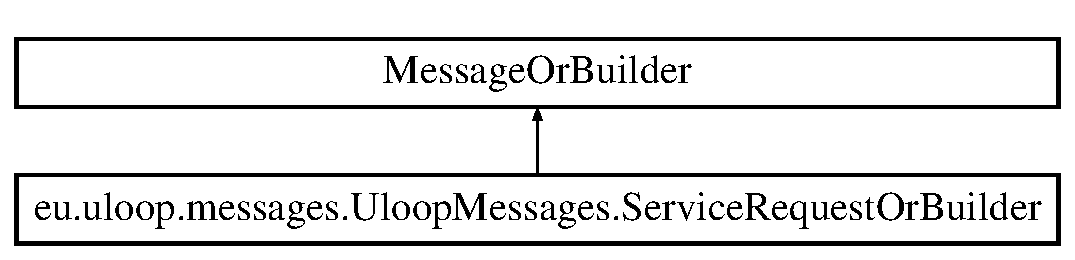
\includegraphics[height=2.000000cm]{interfaceeu_1_1uloop_1_1messages_1_1UloopMessages_1_1ServiceRequestOrBuilder}
\end{center}
\end{figure}
\subsection*{Public Member Functions}
\begin{DoxyCompactItemize}
\item 
boolean \hyperlink{interfaceeu_1_1uloop_1_1messages_1_1UloopMessages_1_1ServiceRequestOrBuilder_a0f44902e7eaea31184396c29b7ae52b5}{has\+Cryptoid} ()
\item 
com.\+google.\+protobuf.\+Byte\+String \hyperlink{interfaceeu_1_1uloop_1_1messages_1_1UloopMessages_1_1ServiceRequestOrBuilder_a9edd5e62cb1ac81212d2a37dbfdfca54}{get\+Cryptoid} ()
\item 
boolean \hyperlink{interfaceeu_1_1uloop_1_1messages_1_1UloopMessages_1_1ServiceRequestOrBuilder_ad12fc9d9a1c9864ae16955bf6b11eb26}{has\+Username} ()
\item 
com.\+google.\+protobuf.\+Byte\+String \hyperlink{interfaceeu_1_1uloop_1_1messages_1_1UloopMessages_1_1ServiceRequestOrBuilder_ab46733bf116ad935e146081135de405e}{get\+Username} ()
\item 
boolean \hyperlink{interfaceeu_1_1uloop_1_1messages_1_1UloopMessages_1_1ServiceRequestOrBuilder_aadde4512967ea6326a9dadff2e0f8f5d}{has\+Password} ()
\item 
com.\+google.\+protobuf.\+Byte\+String \hyperlink{interfaceeu_1_1uloop_1_1messages_1_1UloopMessages_1_1ServiceRequestOrBuilder_ac11bd89c8d0bda5eb312514a5b0e4310}{get\+Password} ()
\item 
boolean \hyperlink{interfaceeu_1_1uloop_1_1messages_1_1UloopMessages_1_1ServiceRequestOrBuilder_a492ea43b826970ad5442191915b0cdad}{has\+Tokens} ()
\item 
double \hyperlink{interfaceeu_1_1uloop_1_1messages_1_1UloopMessages_1_1ServiceRequestOrBuilder_ad147fe14d13b92efec77c52775140753}{get\+Tokens} ()
\item 
boolean \hyperlink{interfaceeu_1_1uloop_1_1messages_1_1UloopMessages_1_1ServiceRequestOrBuilder_a755f19bd870bfecf5d4fd19ff3e46c62}{has\+Promise\+Of\+Payment} ()
\item 
com.\+google.\+protobuf.\+Byte\+String \hyperlink{interfaceeu_1_1uloop_1_1messages_1_1UloopMessages_1_1ServiceRequestOrBuilder_a791bc1d4098a4febbf2908b3c535fb5f}{get\+Promise\+Of\+Payment} ()
\end{DoxyCompactItemize}


\subsection{Member Function Documentation}
\hypertarget{interfaceeu_1_1uloop_1_1messages_1_1UloopMessages_1_1ServiceRequestOrBuilder_a9edd5e62cb1ac81212d2a37dbfdfca54}{\index{eu\+::uloop\+::messages\+::\+Uloop\+Messages\+::\+Service\+Request\+Or\+Builder@{eu\+::uloop\+::messages\+::\+Uloop\+Messages\+::\+Service\+Request\+Or\+Builder}!get\+Cryptoid@{get\+Cryptoid}}
\index{get\+Cryptoid@{get\+Cryptoid}!eu\+::uloop\+::messages\+::\+Uloop\+Messages\+::\+Service\+Request\+Or\+Builder@{eu\+::uloop\+::messages\+::\+Uloop\+Messages\+::\+Service\+Request\+Or\+Builder}}
\subsubsection[{get\+Cryptoid}]{\setlength{\rightskip}{0pt plus 5cm}com.\+google.\+protobuf.\+Byte\+String eu.\+uloop.\+messages.\+Uloop\+Messages.\+Service\+Request\+Or\+Builder.\+get\+Cryptoid (
\begin{DoxyParamCaption}
{}
\end{DoxyParamCaption}
)}}\label{interfaceeu_1_1uloop_1_1messages_1_1UloopMessages_1_1ServiceRequestOrBuilder_a9edd5e62cb1ac81212d2a37dbfdfca54}
\hypertarget{interfaceeu_1_1uloop_1_1messages_1_1UloopMessages_1_1ServiceRequestOrBuilder_ac11bd89c8d0bda5eb312514a5b0e4310}{\index{eu\+::uloop\+::messages\+::\+Uloop\+Messages\+::\+Service\+Request\+Or\+Builder@{eu\+::uloop\+::messages\+::\+Uloop\+Messages\+::\+Service\+Request\+Or\+Builder}!get\+Password@{get\+Password}}
\index{get\+Password@{get\+Password}!eu\+::uloop\+::messages\+::\+Uloop\+Messages\+::\+Service\+Request\+Or\+Builder@{eu\+::uloop\+::messages\+::\+Uloop\+Messages\+::\+Service\+Request\+Or\+Builder}}
\subsubsection[{get\+Password}]{\setlength{\rightskip}{0pt plus 5cm}com.\+google.\+protobuf.\+Byte\+String eu.\+uloop.\+messages.\+Uloop\+Messages.\+Service\+Request\+Or\+Builder.\+get\+Password (
\begin{DoxyParamCaption}
{}
\end{DoxyParamCaption}
)}}\label{interfaceeu_1_1uloop_1_1messages_1_1UloopMessages_1_1ServiceRequestOrBuilder_ac11bd89c8d0bda5eb312514a5b0e4310}
\hypertarget{interfaceeu_1_1uloop_1_1messages_1_1UloopMessages_1_1ServiceRequestOrBuilder_a791bc1d4098a4febbf2908b3c535fb5f}{\index{eu\+::uloop\+::messages\+::\+Uloop\+Messages\+::\+Service\+Request\+Or\+Builder@{eu\+::uloop\+::messages\+::\+Uloop\+Messages\+::\+Service\+Request\+Or\+Builder}!get\+Promise\+Of\+Payment@{get\+Promise\+Of\+Payment}}
\index{get\+Promise\+Of\+Payment@{get\+Promise\+Of\+Payment}!eu\+::uloop\+::messages\+::\+Uloop\+Messages\+::\+Service\+Request\+Or\+Builder@{eu\+::uloop\+::messages\+::\+Uloop\+Messages\+::\+Service\+Request\+Or\+Builder}}
\subsubsection[{get\+Promise\+Of\+Payment}]{\setlength{\rightskip}{0pt plus 5cm}com.\+google.\+protobuf.\+Byte\+String eu.\+uloop.\+messages.\+Uloop\+Messages.\+Service\+Request\+Or\+Builder.\+get\+Promise\+Of\+Payment (
\begin{DoxyParamCaption}
{}
\end{DoxyParamCaption}
)}}\label{interfaceeu_1_1uloop_1_1messages_1_1UloopMessages_1_1ServiceRequestOrBuilder_a791bc1d4098a4febbf2908b3c535fb5f}
\hypertarget{interfaceeu_1_1uloop_1_1messages_1_1UloopMessages_1_1ServiceRequestOrBuilder_ad147fe14d13b92efec77c52775140753}{\index{eu\+::uloop\+::messages\+::\+Uloop\+Messages\+::\+Service\+Request\+Or\+Builder@{eu\+::uloop\+::messages\+::\+Uloop\+Messages\+::\+Service\+Request\+Or\+Builder}!get\+Tokens@{get\+Tokens}}
\index{get\+Tokens@{get\+Tokens}!eu\+::uloop\+::messages\+::\+Uloop\+Messages\+::\+Service\+Request\+Or\+Builder@{eu\+::uloop\+::messages\+::\+Uloop\+Messages\+::\+Service\+Request\+Or\+Builder}}
\subsubsection[{get\+Tokens}]{\setlength{\rightskip}{0pt plus 5cm}double eu.\+uloop.\+messages.\+Uloop\+Messages.\+Service\+Request\+Or\+Builder.\+get\+Tokens (
\begin{DoxyParamCaption}
{}
\end{DoxyParamCaption}
)}}\label{interfaceeu_1_1uloop_1_1messages_1_1UloopMessages_1_1ServiceRequestOrBuilder_ad147fe14d13b92efec77c52775140753}
\hypertarget{interfaceeu_1_1uloop_1_1messages_1_1UloopMessages_1_1ServiceRequestOrBuilder_ab46733bf116ad935e146081135de405e}{\index{eu\+::uloop\+::messages\+::\+Uloop\+Messages\+::\+Service\+Request\+Or\+Builder@{eu\+::uloop\+::messages\+::\+Uloop\+Messages\+::\+Service\+Request\+Or\+Builder}!get\+Username@{get\+Username}}
\index{get\+Username@{get\+Username}!eu\+::uloop\+::messages\+::\+Uloop\+Messages\+::\+Service\+Request\+Or\+Builder@{eu\+::uloop\+::messages\+::\+Uloop\+Messages\+::\+Service\+Request\+Or\+Builder}}
\subsubsection[{get\+Username}]{\setlength{\rightskip}{0pt plus 5cm}com.\+google.\+protobuf.\+Byte\+String eu.\+uloop.\+messages.\+Uloop\+Messages.\+Service\+Request\+Or\+Builder.\+get\+Username (
\begin{DoxyParamCaption}
{}
\end{DoxyParamCaption}
)}}\label{interfaceeu_1_1uloop_1_1messages_1_1UloopMessages_1_1ServiceRequestOrBuilder_ab46733bf116ad935e146081135de405e}
\hypertarget{interfaceeu_1_1uloop_1_1messages_1_1UloopMessages_1_1ServiceRequestOrBuilder_a0f44902e7eaea31184396c29b7ae52b5}{\index{eu\+::uloop\+::messages\+::\+Uloop\+Messages\+::\+Service\+Request\+Or\+Builder@{eu\+::uloop\+::messages\+::\+Uloop\+Messages\+::\+Service\+Request\+Or\+Builder}!has\+Cryptoid@{has\+Cryptoid}}
\index{has\+Cryptoid@{has\+Cryptoid}!eu\+::uloop\+::messages\+::\+Uloop\+Messages\+::\+Service\+Request\+Or\+Builder@{eu\+::uloop\+::messages\+::\+Uloop\+Messages\+::\+Service\+Request\+Or\+Builder}}
\subsubsection[{has\+Cryptoid}]{\setlength{\rightskip}{0pt plus 5cm}boolean eu.\+uloop.\+messages.\+Uloop\+Messages.\+Service\+Request\+Or\+Builder.\+has\+Cryptoid (
\begin{DoxyParamCaption}
{}
\end{DoxyParamCaption}
)}}\label{interfaceeu_1_1uloop_1_1messages_1_1UloopMessages_1_1ServiceRequestOrBuilder_a0f44902e7eaea31184396c29b7ae52b5}
\hypertarget{interfaceeu_1_1uloop_1_1messages_1_1UloopMessages_1_1ServiceRequestOrBuilder_aadde4512967ea6326a9dadff2e0f8f5d}{\index{eu\+::uloop\+::messages\+::\+Uloop\+Messages\+::\+Service\+Request\+Or\+Builder@{eu\+::uloop\+::messages\+::\+Uloop\+Messages\+::\+Service\+Request\+Or\+Builder}!has\+Password@{has\+Password}}
\index{has\+Password@{has\+Password}!eu\+::uloop\+::messages\+::\+Uloop\+Messages\+::\+Service\+Request\+Or\+Builder@{eu\+::uloop\+::messages\+::\+Uloop\+Messages\+::\+Service\+Request\+Or\+Builder}}
\subsubsection[{has\+Password}]{\setlength{\rightskip}{0pt plus 5cm}boolean eu.\+uloop.\+messages.\+Uloop\+Messages.\+Service\+Request\+Or\+Builder.\+has\+Password (
\begin{DoxyParamCaption}
{}
\end{DoxyParamCaption}
)}}\label{interfaceeu_1_1uloop_1_1messages_1_1UloopMessages_1_1ServiceRequestOrBuilder_aadde4512967ea6326a9dadff2e0f8f5d}
\hypertarget{interfaceeu_1_1uloop_1_1messages_1_1UloopMessages_1_1ServiceRequestOrBuilder_a755f19bd870bfecf5d4fd19ff3e46c62}{\index{eu\+::uloop\+::messages\+::\+Uloop\+Messages\+::\+Service\+Request\+Or\+Builder@{eu\+::uloop\+::messages\+::\+Uloop\+Messages\+::\+Service\+Request\+Or\+Builder}!has\+Promise\+Of\+Payment@{has\+Promise\+Of\+Payment}}
\index{has\+Promise\+Of\+Payment@{has\+Promise\+Of\+Payment}!eu\+::uloop\+::messages\+::\+Uloop\+Messages\+::\+Service\+Request\+Or\+Builder@{eu\+::uloop\+::messages\+::\+Uloop\+Messages\+::\+Service\+Request\+Or\+Builder}}
\subsubsection[{has\+Promise\+Of\+Payment}]{\setlength{\rightskip}{0pt plus 5cm}boolean eu.\+uloop.\+messages.\+Uloop\+Messages.\+Service\+Request\+Or\+Builder.\+has\+Promise\+Of\+Payment (
\begin{DoxyParamCaption}
{}
\end{DoxyParamCaption}
)}}\label{interfaceeu_1_1uloop_1_1messages_1_1UloopMessages_1_1ServiceRequestOrBuilder_a755f19bd870bfecf5d4fd19ff3e46c62}
\hypertarget{interfaceeu_1_1uloop_1_1messages_1_1UloopMessages_1_1ServiceRequestOrBuilder_a492ea43b826970ad5442191915b0cdad}{\index{eu\+::uloop\+::messages\+::\+Uloop\+Messages\+::\+Service\+Request\+Or\+Builder@{eu\+::uloop\+::messages\+::\+Uloop\+Messages\+::\+Service\+Request\+Or\+Builder}!has\+Tokens@{has\+Tokens}}
\index{has\+Tokens@{has\+Tokens}!eu\+::uloop\+::messages\+::\+Uloop\+Messages\+::\+Service\+Request\+Or\+Builder@{eu\+::uloop\+::messages\+::\+Uloop\+Messages\+::\+Service\+Request\+Or\+Builder}}
\subsubsection[{has\+Tokens}]{\setlength{\rightskip}{0pt plus 5cm}boolean eu.\+uloop.\+messages.\+Uloop\+Messages.\+Service\+Request\+Or\+Builder.\+has\+Tokens (
\begin{DoxyParamCaption}
{}
\end{DoxyParamCaption}
)}}\label{interfaceeu_1_1uloop_1_1messages_1_1UloopMessages_1_1ServiceRequestOrBuilder_a492ea43b826970ad5442191915b0cdad}
\hypertarget{interfaceeu_1_1uloop_1_1messages_1_1UloopMessages_1_1ServiceRequestOrBuilder_ad12fc9d9a1c9864ae16955bf6b11eb26}{\index{eu\+::uloop\+::messages\+::\+Uloop\+Messages\+::\+Service\+Request\+Or\+Builder@{eu\+::uloop\+::messages\+::\+Uloop\+Messages\+::\+Service\+Request\+Or\+Builder}!has\+Username@{has\+Username}}
\index{has\+Username@{has\+Username}!eu\+::uloop\+::messages\+::\+Uloop\+Messages\+::\+Service\+Request\+Or\+Builder@{eu\+::uloop\+::messages\+::\+Uloop\+Messages\+::\+Service\+Request\+Or\+Builder}}
\subsubsection[{has\+Username}]{\setlength{\rightskip}{0pt plus 5cm}boolean eu.\+uloop.\+messages.\+Uloop\+Messages.\+Service\+Request\+Or\+Builder.\+has\+Username (
\begin{DoxyParamCaption}
{}
\end{DoxyParamCaption}
)}}\label{interfaceeu_1_1uloop_1_1messages_1_1UloopMessages_1_1ServiceRequestOrBuilder_ad12fc9d9a1c9864ae16955bf6b11eb26}


The documentation for this interface was generated from the following file\+:\begin{DoxyCompactItemize}
\item 
src/eu/uloop/messages/\hyperlink{UloopMessages_8java}{Uloop\+Messages.\+java}\end{DoxyCompactItemize}

\hypertarget{interfaceeu_1_1uloop_1_1messages_1_1UloopMessages_1_1ServiceUpdateOrBuilder}{\section{eu.\+uloop.\+messages.\+Uloop\+Messages.\+Service\+Update\+Or\+Builder Interface Reference}
\label{interfaceeu_1_1uloop_1_1messages_1_1UloopMessages_1_1ServiceUpdateOrBuilder}\index{eu.\+uloop.\+messages.\+Uloop\+Messages.\+Service\+Update\+Or\+Builder@{eu.\+uloop.\+messages.\+Uloop\+Messages.\+Service\+Update\+Or\+Builder}}
}
Inheritance diagram for eu.\+uloop.\+messages.\+Uloop\+Messages.\+Service\+Update\+Or\+Builder\+:\begin{figure}[H]
\begin{center}
\leavevmode
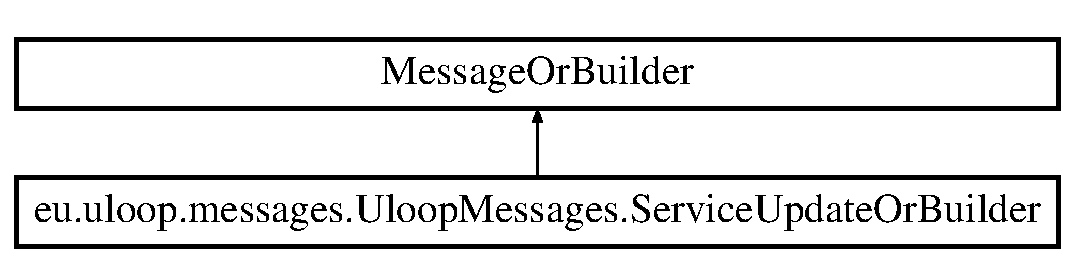
\includegraphics[height=2.000000cm]{interfaceeu_1_1uloop_1_1messages_1_1UloopMessages_1_1ServiceUpdateOrBuilder}
\end{center}
\end{figure}
\subsection*{Public Member Functions}
\begin{DoxyCompactItemize}
\item 
boolean \hyperlink{interfaceeu_1_1uloop_1_1messages_1_1UloopMessages_1_1ServiceUpdateOrBuilder_a15241d25a1c3db88ecb538ca988270df}{has\+Cryptoid} ()
\item 
com.\+google.\+protobuf.\+Byte\+String \hyperlink{interfaceeu_1_1uloop_1_1messages_1_1UloopMessages_1_1ServiceUpdateOrBuilder_a1377c7c0cf844b024a8a2c882a306ab0}{get\+Cryptoid} ()
\end{DoxyCompactItemize}


\subsection{Member Function Documentation}
\hypertarget{interfaceeu_1_1uloop_1_1messages_1_1UloopMessages_1_1ServiceUpdateOrBuilder_a1377c7c0cf844b024a8a2c882a306ab0}{\index{eu\+::uloop\+::messages\+::\+Uloop\+Messages\+::\+Service\+Update\+Or\+Builder@{eu\+::uloop\+::messages\+::\+Uloop\+Messages\+::\+Service\+Update\+Or\+Builder}!get\+Cryptoid@{get\+Cryptoid}}
\index{get\+Cryptoid@{get\+Cryptoid}!eu\+::uloop\+::messages\+::\+Uloop\+Messages\+::\+Service\+Update\+Or\+Builder@{eu\+::uloop\+::messages\+::\+Uloop\+Messages\+::\+Service\+Update\+Or\+Builder}}
\subsubsection[{get\+Cryptoid}]{\setlength{\rightskip}{0pt plus 5cm}com.\+google.\+protobuf.\+Byte\+String eu.\+uloop.\+messages.\+Uloop\+Messages.\+Service\+Update\+Or\+Builder.\+get\+Cryptoid (
\begin{DoxyParamCaption}
{}
\end{DoxyParamCaption}
)}}\label{interfaceeu_1_1uloop_1_1messages_1_1UloopMessages_1_1ServiceUpdateOrBuilder_a1377c7c0cf844b024a8a2c882a306ab0}
\hypertarget{interfaceeu_1_1uloop_1_1messages_1_1UloopMessages_1_1ServiceUpdateOrBuilder_a15241d25a1c3db88ecb538ca988270df}{\index{eu\+::uloop\+::messages\+::\+Uloop\+Messages\+::\+Service\+Update\+Or\+Builder@{eu\+::uloop\+::messages\+::\+Uloop\+Messages\+::\+Service\+Update\+Or\+Builder}!has\+Cryptoid@{has\+Cryptoid}}
\index{has\+Cryptoid@{has\+Cryptoid}!eu\+::uloop\+::messages\+::\+Uloop\+Messages\+::\+Service\+Update\+Or\+Builder@{eu\+::uloop\+::messages\+::\+Uloop\+Messages\+::\+Service\+Update\+Or\+Builder}}
\subsubsection[{has\+Cryptoid}]{\setlength{\rightskip}{0pt plus 5cm}boolean eu.\+uloop.\+messages.\+Uloop\+Messages.\+Service\+Update\+Or\+Builder.\+has\+Cryptoid (
\begin{DoxyParamCaption}
{}
\end{DoxyParamCaption}
)}}\label{interfaceeu_1_1uloop_1_1messages_1_1UloopMessages_1_1ServiceUpdateOrBuilder_a15241d25a1c3db88ecb538ca988270df}


The documentation for this interface was generated from the following file\+:\begin{DoxyCompactItemize}
\item 
src/eu/uloop/messages/\hyperlink{UloopMessages_8java}{Uloop\+Messages.\+java}\end{DoxyCompactItemize}

\hypertarget{interfaceeu_1_1uloop_1_1messages_1_1UloopMessages_1_1TrustInformationReplyOrBuilder}{\section{eu.\+uloop.\+messages.\+Uloop\+Messages.\+Trust\+Information\+Reply\+Or\+Builder Interface Reference}
\label{interfaceeu_1_1uloop_1_1messages_1_1UloopMessages_1_1TrustInformationReplyOrBuilder}\index{eu.\+uloop.\+messages.\+Uloop\+Messages.\+Trust\+Information\+Reply\+Or\+Builder@{eu.\+uloop.\+messages.\+Uloop\+Messages.\+Trust\+Information\+Reply\+Or\+Builder}}
}
Inheritance diagram for eu.\+uloop.\+messages.\+Uloop\+Messages.\+Trust\+Information\+Reply\+Or\+Builder\+:\begin{figure}[H]
\begin{center}
\leavevmode
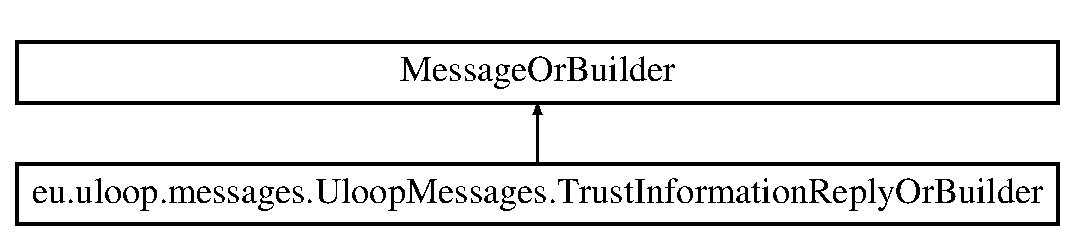
\includegraphics[height=2.000000cm]{interfaceeu_1_1uloop_1_1messages_1_1UloopMessages_1_1TrustInformationReplyOrBuilder}
\end{center}
\end{figure}
\subsection*{Public Member Functions}
\begin{DoxyCompactItemize}
\item 
boolean \hyperlink{interfaceeu_1_1uloop_1_1messages_1_1UloopMessages_1_1TrustInformationReplyOrBuilder_aee12fe0d59ab7bc2236e99a1fd27f122}{has\+Token} ()
\item 
double \hyperlink{interfaceeu_1_1uloop_1_1messages_1_1UloopMessages_1_1TrustInformationReplyOrBuilder_aa51a4461cca37c8da462d8e764db827d}{get\+Token} ()
\end{DoxyCompactItemize}


\subsection{Member Function Documentation}
\hypertarget{interfaceeu_1_1uloop_1_1messages_1_1UloopMessages_1_1TrustInformationReplyOrBuilder_aa51a4461cca37c8da462d8e764db827d}{\index{eu\+::uloop\+::messages\+::\+Uloop\+Messages\+::\+Trust\+Information\+Reply\+Or\+Builder@{eu\+::uloop\+::messages\+::\+Uloop\+Messages\+::\+Trust\+Information\+Reply\+Or\+Builder}!get\+Token@{get\+Token}}
\index{get\+Token@{get\+Token}!eu\+::uloop\+::messages\+::\+Uloop\+Messages\+::\+Trust\+Information\+Reply\+Or\+Builder@{eu\+::uloop\+::messages\+::\+Uloop\+Messages\+::\+Trust\+Information\+Reply\+Or\+Builder}}
\subsubsection[{get\+Token}]{\setlength{\rightskip}{0pt plus 5cm}double eu.\+uloop.\+messages.\+Uloop\+Messages.\+Trust\+Information\+Reply\+Or\+Builder.\+get\+Token (
\begin{DoxyParamCaption}
{}
\end{DoxyParamCaption}
)}}\label{interfaceeu_1_1uloop_1_1messages_1_1UloopMessages_1_1TrustInformationReplyOrBuilder_aa51a4461cca37c8da462d8e764db827d}
\hypertarget{interfaceeu_1_1uloop_1_1messages_1_1UloopMessages_1_1TrustInformationReplyOrBuilder_aee12fe0d59ab7bc2236e99a1fd27f122}{\index{eu\+::uloop\+::messages\+::\+Uloop\+Messages\+::\+Trust\+Information\+Reply\+Or\+Builder@{eu\+::uloop\+::messages\+::\+Uloop\+Messages\+::\+Trust\+Information\+Reply\+Or\+Builder}!has\+Token@{has\+Token}}
\index{has\+Token@{has\+Token}!eu\+::uloop\+::messages\+::\+Uloop\+Messages\+::\+Trust\+Information\+Reply\+Or\+Builder@{eu\+::uloop\+::messages\+::\+Uloop\+Messages\+::\+Trust\+Information\+Reply\+Or\+Builder}}
\subsubsection[{has\+Token}]{\setlength{\rightskip}{0pt plus 5cm}boolean eu.\+uloop.\+messages.\+Uloop\+Messages.\+Trust\+Information\+Reply\+Or\+Builder.\+has\+Token (
\begin{DoxyParamCaption}
{}
\end{DoxyParamCaption}
)}}\label{interfaceeu_1_1uloop_1_1messages_1_1UloopMessages_1_1TrustInformationReplyOrBuilder_aee12fe0d59ab7bc2236e99a1fd27f122}


The documentation for this interface was generated from the following file\+:\begin{DoxyCompactItemize}
\item 
src/eu/uloop/messages/\hyperlink{UloopMessages_8java}{Uloop\+Messages.\+java}\end{DoxyCompactItemize}

\hypertarget{interfaceeu_1_1uloop_1_1messages_1_1UloopMessages_1_1TrustInformationRequestOrBuilder}{\section{eu.\+uloop.\+messages.\+Uloop\+Messages.\+Trust\+Information\+Request\+Or\+Builder Interface Reference}
\label{interfaceeu_1_1uloop_1_1messages_1_1UloopMessages_1_1TrustInformationRequestOrBuilder}\index{eu.\+uloop.\+messages.\+Uloop\+Messages.\+Trust\+Information\+Request\+Or\+Builder@{eu.\+uloop.\+messages.\+Uloop\+Messages.\+Trust\+Information\+Request\+Or\+Builder}}
}
Inheritance diagram for eu.\+uloop.\+messages.\+Uloop\+Messages.\+Trust\+Information\+Request\+Or\+Builder\+:\begin{figure}[H]
\begin{center}
\leavevmode
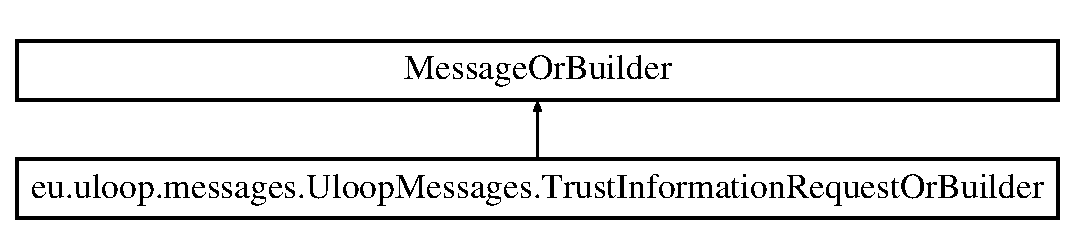
\includegraphics[height=2.000000cm]{interfaceeu_1_1uloop_1_1messages_1_1UloopMessages_1_1TrustInformationRequestOrBuilder}
\end{center}
\end{figure}
\subsection*{Public Member Functions}
\begin{DoxyCompactItemize}
\item 
boolean \hyperlink{interfaceeu_1_1uloop_1_1messages_1_1UloopMessages_1_1TrustInformationRequestOrBuilder_a3a611d6db786591af6cd754e158e934b}{has\+Map} ()
\item 
com.\+google.\+protobuf.\+Byte\+String \hyperlink{interfaceeu_1_1uloop_1_1messages_1_1UloopMessages_1_1TrustInformationRequestOrBuilder_aaf3aef372874a0615556004381c6d855}{get\+Map} ()
\end{DoxyCompactItemize}


\subsection{Member Function Documentation}
\hypertarget{interfaceeu_1_1uloop_1_1messages_1_1UloopMessages_1_1TrustInformationRequestOrBuilder_aaf3aef372874a0615556004381c6d855}{\index{eu\+::uloop\+::messages\+::\+Uloop\+Messages\+::\+Trust\+Information\+Request\+Or\+Builder@{eu\+::uloop\+::messages\+::\+Uloop\+Messages\+::\+Trust\+Information\+Request\+Or\+Builder}!get\+Map@{get\+Map}}
\index{get\+Map@{get\+Map}!eu\+::uloop\+::messages\+::\+Uloop\+Messages\+::\+Trust\+Information\+Request\+Or\+Builder@{eu\+::uloop\+::messages\+::\+Uloop\+Messages\+::\+Trust\+Information\+Request\+Or\+Builder}}
\subsubsection[{get\+Map}]{\setlength{\rightskip}{0pt plus 5cm}com.\+google.\+protobuf.\+Byte\+String eu.\+uloop.\+messages.\+Uloop\+Messages.\+Trust\+Information\+Request\+Or\+Builder.\+get\+Map (
\begin{DoxyParamCaption}
{}
\end{DoxyParamCaption}
)}}\label{interfaceeu_1_1uloop_1_1messages_1_1UloopMessages_1_1TrustInformationRequestOrBuilder_aaf3aef372874a0615556004381c6d855}
\hypertarget{interfaceeu_1_1uloop_1_1messages_1_1UloopMessages_1_1TrustInformationRequestOrBuilder_a3a611d6db786591af6cd754e158e934b}{\index{eu\+::uloop\+::messages\+::\+Uloop\+Messages\+::\+Trust\+Information\+Request\+Or\+Builder@{eu\+::uloop\+::messages\+::\+Uloop\+Messages\+::\+Trust\+Information\+Request\+Or\+Builder}!has\+Map@{has\+Map}}
\index{has\+Map@{has\+Map}!eu\+::uloop\+::messages\+::\+Uloop\+Messages\+::\+Trust\+Information\+Request\+Or\+Builder@{eu\+::uloop\+::messages\+::\+Uloop\+Messages\+::\+Trust\+Information\+Request\+Or\+Builder}}
\subsubsection[{has\+Map}]{\setlength{\rightskip}{0pt plus 5cm}boolean eu.\+uloop.\+messages.\+Uloop\+Messages.\+Trust\+Information\+Request\+Or\+Builder.\+has\+Map (
\begin{DoxyParamCaption}
{}
\end{DoxyParamCaption}
)}}\label{interfaceeu_1_1uloop_1_1messages_1_1UloopMessages_1_1TrustInformationRequestOrBuilder_a3a611d6db786591af6cd754e158e934b}


The documentation for this interface was generated from the following file\+:\begin{DoxyCompactItemize}
\item 
src/eu/uloop/messages/\hyperlink{UloopMessages_8java}{Uloop\+Messages.\+java}\end{DoxyCompactItemize}

\hypertarget{interfaceeu_1_1uloop_1_1messages_1_1UloopMessages_1_1TrustMessageOrBuilder}{\section{eu.\+uloop.\+messages.\+Uloop\+Messages.\+Trust\+Message\+Or\+Builder Interface Reference}
\label{interfaceeu_1_1uloop_1_1messages_1_1UloopMessages_1_1TrustMessageOrBuilder}\index{eu.\+uloop.\+messages.\+Uloop\+Messages.\+Trust\+Message\+Or\+Builder@{eu.\+uloop.\+messages.\+Uloop\+Messages.\+Trust\+Message\+Or\+Builder}}
}
Inheritance diagram for eu.\+uloop.\+messages.\+Uloop\+Messages.\+Trust\+Message\+Or\+Builder\+:\begin{figure}[H]
\begin{center}
\leavevmode
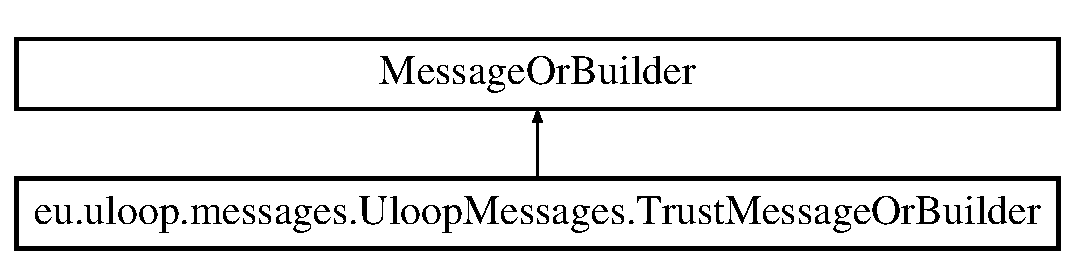
\includegraphics[height=2.000000cm]{interfaceeu_1_1uloop_1_1messages_1_1UloopMessages_1_1TrustMessageOrBuilder}
\end{center}
\end{figure}
\subsection*{Public Member Functions}
\begin{DoxyCompactItemize}
\item 
boolean \hyperlink{interfaceeu_1_1uloop_1_1messages_1_1UloopMessages_1_1TrustMessageOrBuilder_a6dd194c5f9689dd36b261d51503368ae}{has\+Treq} ()
\item 
eu.\+uloop.\+messages.\+Uloop\+Messages.\+Trust\+Information\+Request \hyperlink{interfaceeu_1_1uloop_1_1messages_1_1UloopMessages_1_1TrustMessageOrBuilder_aded15eba27d62d7e494f1b4a9b580f83}{get\+Treq} ()
\item 
\hyperlink{interfaceeu_1_1uloop_1_1messages_1_1UloopMessages_1_1TrustInformationRequestOrBuilder}{eu.\+uloop.\+messages.\+Uloop\+Messages.\+Trust\+Information\+Request\+Or\+Builder} \hyperlink{interfaceeu_1_1uloop_1_1messages_1_1UloopMessages_1_1TrustMessageOrBuilder_ae7609c5f196f96a6797004a1113c1071}{get\+Treq\+Or\+Builder} ()
\item 
boolean \hyperlink{interfaceeu_1_1uloop_1_1messages_1_1UloopMessages_1_1TrustMessageOrBuilder_a8824f4115ae760aff8cc83c3abbcbb73}{has\+Trep} ()
\item 
eu.\+uloop.\+messages.\+Uloop\+Messages.\+Trust\+Information\+Reply \hyperlink{interfaceeu_1_1uloop_1_1messages_1_1UloopMessages_1_1TrustMessageOrBuilder_a33ec4d7d4ca00c080b1fd0eba629e96b}{get\+Trep} ()
\item 
\hyperlink{interfaceeu_1_1uloop_1_1messages_1_1UloopMessages_1_1TrustInformationReplyOrBuilder}{eu.\+uloop.\+messages.\+Uloop\+Messages.\+Trust\+Information\+Reply\+Or\+Builder} \hyperlink{interfaceeu_1_1uloop_1_1messages_1_1UloopMessages_1_1TrustMessageOrBuilder_a0720d85fe01f7b0e9535f8fd42003ba7}{get\+Trep\+Or\+Builder} ()
\end{DoxyCompactItemize}


\subsection{Member Function Documentation}
\hypertarget{interfaceeu_1_1uloop_1_1messages_1_1UloopMessages_1_1TrustMessageOrBuilder_a33ec4d7d4ca00c080b1fd0eba629e96b}{\index{eu\+::uloop\+::messages\+::\+Uloop\+Messages\+::\+Trust\+Message\+Or\+Builder@{eu\+::uloop\+::messages\+::\+Uloop\+Messages\+::\+Trust\+Message\+Or\+Builder}!get\+Trep@{get\+Trep}}
\index{get\+Trep@{get\+Trep}!eu\+::uloop\+::messages\+::\+Uloop\+Messages\+::\+Trust\+Message\+Or\+Builder@{eu\+::uloop\+::messages\+::\+Uloop\+Messages\+::\+Trust\+Message\+Or\+Builder}}
\subsubsection[{get\+Trep}]{\setlength{\rightskip}{0pt plus 5cm}eu.\+uloop.\+messages.\+Uloop\+Messages.\+Trust\+Information\+Reply eu.\+uloop.\+messages.\+Uloop\+Messages.\+Trust\+Message\+Or\+Builder.\+get\+Trep (
\begin{DoxyParamCaption}
{}
\end{DoxyParamCaption}
)}}\label{interfaceeu_1_1uloop_1_1messages_1_1UloopMessages_1_1TrustMessageOrBuilder_a33ec4d7d4ca00c080b1fd0eba629e96b}
\hypertarget{interfaceeu_1_1uloop_1_1messages_1_1UloopMessages_1_1TrustMessageOrBuilder_a0720d85fe01f7b0e9535f8fd42003ba7}{\index{eu\+::uloop\+::messages\+::\+Uloop\+Messages\+::\+Trust\+Message\+Or\+Builder@{eu\+::uloop\+::messages\+::\+Uloop\+Messages\+::\+Trust\+Message\+Or\+Builder}!get\+Trep\+Or\+Builder@{get\+Trep\+Or\+Builder}}
\index{get\+Trep\+Or\+Builder@{get\+Trep\+Or\+Builder}!eu\+::uloop\+::messages\+::\+Uloop\+Messages\+::\+Trust\+Message\+Or\+Builder@{eu\+::uloop\+::messages\+::\+Uloop\+Messages\+::\+Trust\+Message\+Or\+Builder}}
\subsubsection[{get\+Trep\+Or\+Builder}]{\setlength{\rightskip}{0pt plus 5cm}{\bf eu.\+uloop.\+messages.\+Uloop\+Messages.\+Trust\+Information\+Reply\+Or\+Builder} eu.\+uloop.\+messages.\+Uloop\+Messages.\+Trust\+Message\+Or\+Builder.\+get\+Trep\+Or\+Builder (
\begin{DoxyParamCaption}
{}
\end{DoxyParamCaption}
)}}\label{interfaceeu_1_1uloop_1_1messages_1_1UloopMessages_1_1TrustMessageOrBuilder_a0720d85fe01f7b0e9535f8fd42003ba7}
\hypertarget{interfaceeu_1_1uloop_1_1messages_1_1UloopMessages_1_1TrustMessageOrBuilder_aded15eba27d62d7e494f1b4a9b580f83}{\index{eu\+::uloop\+::messages\+::\+Uloop\+Messages\+::\+Trust\+Message\+Or\+Builder@{eu\+::uloop\+::messages\+::\+Uloop\+Messages\+::\+Trust\+Message\+Or\+Builder}!get\+Treq@{get\+Treq}}
\index{get\+Treq@{get\+Treq}!eu\+::uloop\+::messages\+::\+Uloop\+Messages\+::\+Trust\+Message\+Or\+Builder@{eu\+::uloop\+::messages\+::\+Uloop\+Messages\+::\+Trust\+Message\+Or\+Builder}}
\subsubsection[{get\+Treq}]{\setlength{\rightskip}{0pt plus 5cm}eu.\+uloop.\+messages.\+Uloop\+Messages.\+Trust\+Information\+Request eu.\+uloop.\+messages.\+Uloop\+Messages.\+Trust\+Message\+Or\+Builder.\+get\+Treq (
\begin{DoxyParamCaption}
{}
\end{DoxyParamCaption}
)}}\label{interfaceeu_1_1uloop_1_1messages_1_1UloopMessages_1_1TrustMessageOrBuilder_aded15eba27d62d7e494f1b4a9b580f83}
\hypertarget{interfaceeu_1_1uloop_1_1messages_1_1UloopMessages_1_1TrustMessageOrBuilder_ae7609c5f196f96a6797004a1113c1071}{\index{eu\+::uloop\+::messages\+::\+Uloop\+Messages\+::\+Trust\+Message\+Or\+Builder@{eu\+::uloop\+::messages\+::\+Uloop\+Messages\+::\+Trust\+Message\+Or\+Builder}!get\+Treq\+Or\+Builder@{get\+Treq\+Or\+Builder}}
\index{get\+Treq\+Or\+Builder@{get\+Treq\+Or\+Builder}!eu\+::uloop\+::messages\+::\+Uloop\+Messages\+::\+Trust\+Message\+Or\+Builder@{eu\+::uloop\+::messages\+::\+Uloop\+Messages\+::\+Trust\+Message\+Or\+Builder}}
\subsubsection[{get\+Treq\+Or\+Builder}]{\setlength{\rightskip}{0pt plus 5cm}{\bf eu.\+uloop.\+messages.\+Uloop\+Messages.\+Trust\+Information\+Request\+Or\+Builder} eu.\+uloop.\+messages.\+Uloop\+Messages.\+Trust\+Message\+Or\+Builder.\+get\+Treq\+Or\+Builder (
\begin{DoxyParamCaption}
{}
\end{DoxyParamCaption}
)}}\label{interfaceeu_1_1uloop_1_1messages_1_1UloopMessages_1_1TrustMessageOrBuilder_ae7609c5f196f96a6797004a1113c1071}
\hypertarget{interfaceeu_1_1uloop_1_1messages_1_1UloopMessages_1_1TrustMessageOrBuilder_a8824f4115ae760aff8cc83c3abbcbb73}{\index{eu\+::uloop\+::messages\+::\+Uloop\+Messages\+::\+Trust\+Message\+Or\+Builder@{eu\+::uloop\+::messages\+::\+Uloop\+Messages\+::\+Trust\+Message\+Or\+Builder}!has\+Trep@{has\+Trep}}
\index{has\+Trep@{has\+Trep}!eu\+::uloop\+::messages\+::\+Uloop\+Messages\+::\+Trust\+Message\+Or\+Builder@{eu\+::uloop\+::messages\+::\+Uloop\+Messages\+::\+Trust\+Message\+Or\+Builder}}
\subsubsection[{has\+Trep}]{\setlength{\rightskip}{0pt plus 5cm}boolean eu.\+uloop.\+messages.\+Uloop\+Messages.\+Trust\+Message\+Or\+Builder.\+has\+Trep (
\begin{DoxyParamCaption}
{}
\end{DoxyParamCaption}
)}}\label{interfaceeu_1_1uloop_1_1messages_1_1UloopMessages_1_1TrustMessageOrBuilder_a8824f4115ae760aff8cc83c3abbcbb73}
\hypertarget{interfaceeu_1_1uloop_1_1messages_1_1UloopMessages_1_1TrustMessageOrBuilder_a6dd194c5f9689dd36b261d51503368ae}{\index{eu\+::uloop\+::messages\+::\+Uloop\+Messages\+::\+Trust\+Message\+Or\+Builder@{eu\+::uloop\+::messages\+::\+Uloop\+Messages\+::\+Trust\+Message\+Or\+Builder}!has\+Treq@{has\+Treq}}
\index{has\+Treq@{has\+Treq}!eu\+::uloop\+::messages\+::\+Uloop\+Messages\+::\+Trust\+Message\+Or\+Builder@{eu\+::uloop\+::messages\+::\+Uloop\+Messages\+::\+Trust\+Message\+Or\+Builder}}
\subsubsection[{has\+Treq}]{\setlength{\rightskip}{0pt plus 5cm}boolean eu.\+uloop.\+messages.\+Uloop\+Messages.\+Trust\+Message\+Or\+Builder.\+has\+Treq (
\begin{DoxyParamCaption}
{}
\end{DoxyParamCaption}
)}}\label{interfaceeu_1_1uloop_1_1messages_1_1UloopMessages_1_1TrustMessageOrBuilder_a6dd194c5f9689dd36b261d51503368ae}


The documentation for this interface was generated from the following file\+:\begin{DoxyCompactItemize}
\item 
src/eu/uloop/messages/\hyperlink{UloopMessages_8java}{Uloop\+Messages.\+java}\end{DoxyCompactItemize}

\hypertarget{interfacelib_1_1api_1_1UloopAbstractMessage}{\section{lib.\+api.\+Uloop\+Abstract\+Message Interface Reference}
\label{interfacelib_1_1api_1_1UloopAbstractMessage}\index{lib.\+api.\+Uloop\+Abstract\+Message@{lib.\+api.\+Uloop\+Abstract\+Message}}
}
Inheritance diagram for lib.\+api.\+Uloop\+Abstract\+Message\+:\begin{figure}[H]
\begin{center}
\leavevmode
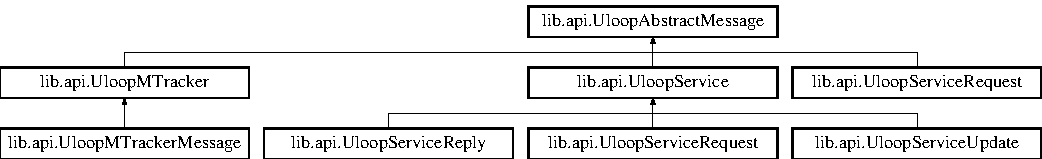
\includegraphics[height=2.142857cm]{interfacelib_1_1api_1_1UloopAbstractMessage}
\end{center}
\end{figure}
\subsection*{Public Member Functions}
\begin{DoxyCompactItemize}
\item 
\hyperlink{interfacelib_1_1api_1_1UloopAbstractMessage}{Uloop\+Abstract\+Message} \hyperlink{interfacelib_1_1api_1_1UloopAbstractMessage_a1a650d00338402b7d2a5f46575241986}{decode} (Uloop\+Message ulm)  throws Runtime\+Exception
\item 
Uloop\+Message.\+Builder \hyperlink{interfacelib_1_1api_1_1UloopAbstractMessage_a00e05a40924dadb7ee429c811628aea3}{encode} ()
\item 
void \hyperlink{interfacelib_1_1api_1_1UloopAbstractMessage_a116bcd258e6e384507888f4a2e2100a9}{print} ()
\end{DoxyCompactItemize}


\subsection{Member Function Documentation}
\hypertarget{interfacelib_1_1api_1_1UloopAbstractMessage_a1a650d00338402b7d2a5f46575241986}{\index{lib\+::api\+::\+Uloop\+Abstract\+Message@{lib\+::api\+::\+Uloop\+Abstract\+Message}!decode@{decode}}
\index{decode@{decode}!lib\+::api\+::\+Uloop\+Abstract\+Message@{lib\+::api\+::\+Uloop\+Abstract\+Message}}
\subsubsection[{decode}]{\setlength{\rightskip}{0pt plus 5cm}{\bf Uloop\+Abstract\+Message} lib.\+api.\+Uloop\+Abstract\+Message.\+decode (
\begin{DoxyParamCaption}
\item[{Uloop\+Message}]{ulm}
\end{DoxyParamCaption}
) throws Runtime\+Exception}}\label{interfacelib_1_1api_1_1UloopAbstractMessage_a1a650d00338402b7d2a5f46575241986}


Implemented in \hyperlink{classlib_1_1api_1_1UloopMTrackerMessage_a3251cbbabd745f22290f334c475d4c97}{lib.\+api.\+Uloop\+M\+Tracker\+Message}, \hyperlink{classlib_1_1api_1_1UloopServiceRequest_a4a8a64d824425f1d326f3be82115ccf2}{lib.\+api.\+Uloop\+Service\+Request}, \hyperlink{classlib_1_1api_1_1UloopServiceReply_a944ecbe5d5a40e6ae48ee884063f5c1d}{lib.\+api.\+Uloop\+Service\+Reply}, and \hyperlink{classlib_1_1api_1_1UloopServiceUpdate_a3bb1384447e9db3372e48356ff5a214f}{lib.\+api.\+Uloop\+Service\+Update}.

\hypertarget{interfacelib_1_1api_1_1UloopAbstractMessage_a00e05a40924dadb7ee429c811628aea3}{\index{lib\+::api\+::\+Uloop\+Abstract\+Message@{lib\+::api\+::\+Uloop\+Abstract\+Message}!encode@{encode}}
\index{encode@{encode}!lib\+::api\+::\+Uloop\+Abstract\+Message@{lib\+::api\+::\+Uloop\+Abstract\+Message}}
\subsubsection[{encode}]{\setlength{\rightskip}{0pt plus 5cm}Uloop\+Message.\+Builder lib.\+api.\+Uloop\+Abstract\+Message.\+encode (
\begin{DoxyParamCaption}
{}
\end{DoxyParamCaption}
)}}\label{interfacelib_1_1api_1_1UloopAbstractMessage_a00e05a40924dadb7ee429c811628aea3}


Implemented in \hyperlink{classlib_1_1api_1_1UloopMTrackerMessage_a9d9ff3e73a53ae13088b52df395de90a}{lib.\+api.\+Uloop\+M\+Tracker\+Message}, \hyperlink{classlib_1_1api_1_1UloopServiceRequest_a13409dd756188327c2885eda6f9a8b17}{lib.\+api.\+Uloop\+Service\+Request}, \hyperlink{classlib_1_1api_1_1UloopServiceReply_a0ca29eaf04dce5493607e010b73f77d4}{lib.\+api.\+Uloop\+Service\+Reply}, and \hyperlink{classlib_1_1api_1_1UloopServiceUpdate_a0933882171971eb0f704101ba19f36f4}{lib.\+api.\+Uloop\+Service\+Update}.

\hypertarget{interfacelib_1_1api_1_1UloopAbstractMessage_a116bcd258e6e384507888f4a2e2100a9}{\index{lib\+::api\+::\+Uloop\+Abstract\+Message@{lib\+::api\+::\+Uloop\+Abstract\+Message}!print@{print}}
\index{print@{print}!lib\+::api\+::\+Uloop\+Abstract\+Message@{lib\+::api\+::\+Uloop\+Abstract\+Message}}
\subsubsection[{print}]{\setlength{\rightskip}{0pt plus 5cm}void lib.\+api.\+Uloop\+Abstract\+Message.\+print (
\begin{DoxyParamCaption}
{}
\end{DoxyParamCaption}
)}}\label{interfacelib_1_1api_1_1UloopAbstractMessage_a116bcd258e6e384507888f4a2e2100a9}


Implemented in \hyperlink{classlib_1_1api_1_1UloopServiceRequest_a297690e00aed1f79499de2c9095fe52c}{lib.\+api.\+Uloop\+Service\+Request}, \hyperlink{classlib_1_1api_1_1UloopMTrackerMessage_ad8747254f5616590148266b72b088421}{lib.\+api.\+Uloop\+M\+Tracker\+Message}, \hyperlink{classlib_1_1api_1_1UloopServiceReply_a825bbcd3250cc8ac980f3eda449c482f}{lib.\+api.\+Uloop\+Service\+Reply}, and \hyperlink{classlib_1_1api_1_1UloopServiceUpdate_a92cf6fa47379c50f0117838e97e7eb9d}{lib.\+api.\+Uloop\+Service\+Update}.



The documentation for this interface was generated from the following file\+:\begin{DoxyCompactItemize}
\item 
src/lib/api/\hyperlink{UloopAbstractMessage_8java}{Uloop\+Abstract\+Message.\+java}\end{DoxyCompactItemize}

\hypertarget{interfaceeu_1_1uloop_1_1messages_1_1UloopMessages_1_1UloopHeaderMessageOrBuilder}{\section{eu.\+uloop.\+messages.\+Uloop\+Messages.\+Uloop\+Header\+Message\+Or\+Builder Interface Reference}
\label{interfaceeu_1_1uloop_1_1messages_1_1UloopMessages_1_1UloopHeaderMessageOrBuilder}\index{eu.\+uloop.\+messages.\+Uloop\+Messages.\+Uloop\+Header\+Message\+Or\+Builder@{eu.\+uloop.\+messages.\+Uloop\+Messages.\+Uloop\+Header\+Message\+Or\+Builder}}
}
Inheritance diagram for eu.\+uloop.\+messages.\+Uloop\+Messages.\+Uloop\+Header\+Message\+Or\+Builder\+:\begin{figure}[H]
\begin{center}
\leavevmode
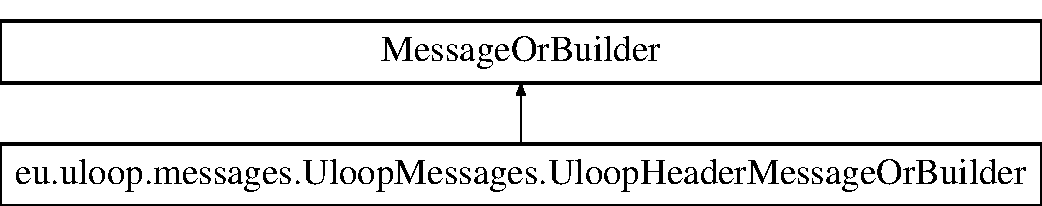
\includegraphics[height=2.000000cm]{interfaceeu_1_1uloop_1_1messages_1_1UloopMessages_1_1UloopHeaderMessageOrBuilder}
\end{center}
\end{figure}
\subsection*{Public Member Functions}
\begin{DoxyCompactItemize}
\item 
boolean \hyperlink{interfaceeu_1_1uloop_1_1messages_1_1UloopMessages_1_1UloopHeaderMessageOrBuilder_aa38365a514f24893ed96f4a2a27078f6}{has\+Length} ()
\item 
int \hyperlink{interfaceeu_1_1uloop_1_1messages_1_1UloopMessages_1_1UloopHeaderMessageOrBuilder_ac927004c4f81b38d8127cfb97f1dd470}{get\+Length} ()
\end{DoxyCompactItemize}


\subsection{Member Function Documentation}
\hypertarget{interfaceeu_1_1uloop_1_1messages_1_1UloopMessages_1_1UloopHeaderMessageOrBuilder_ac927004c4f81b38d8127cfb97f1dd470}{\index{eu\+::uloop\+::messages\+::\+Uloop\+Messages\+::\+Uloop\+Header\+Message\+Or\+Builder@{eu\+::uloop\+::messages\+::\+Uloop\+Messages\+::\+Uloop\+Header\+Message\+Or\+Builder}!get\+Length@{get\+Length}}
\index{get\+Length@{get\+Length}!eu\+::uloop\+::messages\+::\+Uloop\+Messages\+::\+Uloop\+Header\+Message\+Or\+Builder@{eu\+::uloop\+::messages\+::\+Uloop\+Messages\+::\+Uloop\+Header\+Message\+Or\+Builder}}
\subsubsection[{get\+Length}]{\setlength{\rightskip}{0pt plus 5cm}int eu.\+uloop.\+messages.\+Uloop\+Messages.\+Uloop\+Header\+Message\+Or\+Builder.\+get\+Length (
\begin{DoxyParamCaption}
{}
\end{DoxyParamCaption}
)}}\label{interfaceeu_1_1uloop_1_1messages_1_1UloopMessages_1_1UloopHeaderMessageOrBuilder_ac927004c4f81b38d8127cfb97f1dd470}
\hypertarget{interfaceeu_1_1uloop_1_1messages_1_1UloopMessages_1_1UloopHeaderMessageOrBuilder_aa38365a514f24893ed96f4a2a27078f6}{\index{eu\+::uloop\+::messages\+::\+Uloop\+Messages\+::\+Uloop\+Header\+Message\+Or\+Builder@{eu\+::uloop\+::messages\+::\+Uloop\+Messages\+::\+Uloop\+Header\+Message\+Or\+Builder}!has\+Length@{has\+Length}}
\index{has\+Length@{has\+Length}!eu\+::uloop\+::messages\+::\+Uloop\+Messages\+::\+Uloop\+Header\+Message\+Or\+Builder@{eu\+::uloop\+::messages\+::\+Uloop\+Messages\+::\+Uloop\+Header\+Message\+Or\+Builder}}
\subsubsection[{has\+Length}]{\setlength{\rightskip}{0pt plus 5cm}boolean eu.\+uloop.\+messages.\+Uloop\+Messages.\+Uloop\+Header\+Message\+Or\+Builder.\+has\+Length (
\begin{DoxyParamCaption}
{}
\end{DoxyParamCaption}
)}}\label{interfaceeu_1_1uloop_1_1messages_1_1UloopMessages_1_1UloopHeaderMessageOrBuilder_aa38365a514f24893ed96f4a2a27078f6}


The documentation for this interface was generated from the following file\+:\begin{DoxyCompactItemize}
\item 
src/eu/uloop/messages/\hyperlink{UloopMessages_8java}{Uloop\+Messages.\+java}\end{DoxyCompactItemize}

\hypertarget{interfacelib_1_1api_1_1UloopMessageAPI}{\section{lib.\+api.\+Uloop\+Message\+A\+P\+I Interface Reference}
\label{interfacelib_1_1api_1_1UloopMessageAPI}\index{lib.\+api.\+Uloop\+Message\+A\+P\+I@{lib.\+api.\+Uloop\+Message\+A\+P\+I}}
}
Inheritance diagram for lib.\+api.\+Uloop\+Message\+A\+P\+I\+:\begin{figure}[H]
\begin{center}
\leavevmode
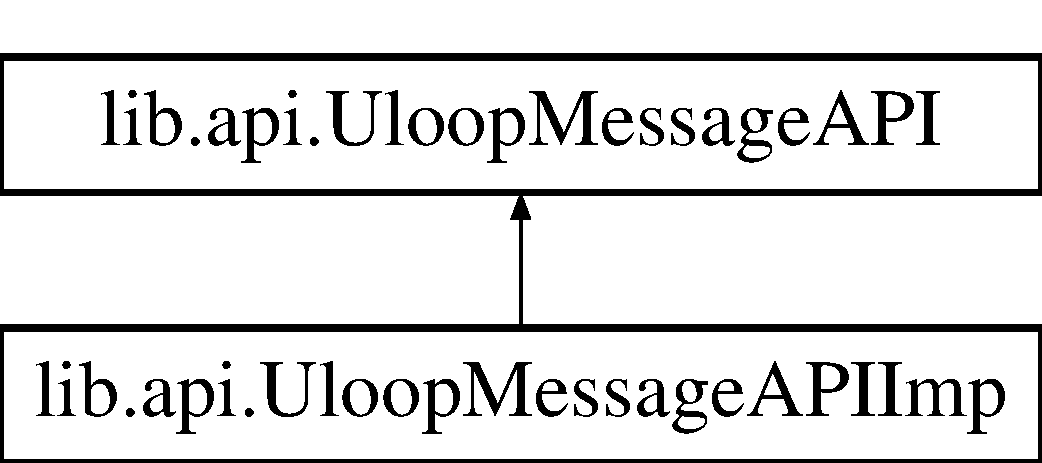
\includegraphics[height=2.000000cm]{interfacelib_1_1api_1_1UloopMessageAPI}
\end{center}
\end{figure}
\subsection*{Public Member Functions}
\begin{DoxyCompactItemize}
\item 
void \hyperlink{interfacelib_1_1api_1_1UloopMessageAPI_a026a74704c323ac8fce79bd9db7084a6}{send\+\_\+service\+\_\+request} (\hyperlink{classlib_1_1api_1_1UloopService}{Uloop\+Service} ulservice)
\item 
\hyperlink{classlib_1_1api_1_1UloopService}{Uloop\+Service} \hyperlink{interfacelib_1_1api_1_1UloopMessageAPI_a7867cdc90ec092d844190a00546de522}{recv\+\_\+service\+\_\+request} ()
\item 
void \hyperlink{interfacelib_1_1api_1_1UloopMessageAPI_a1d2c724d79a4840d2c09f108b23b19cd}{send\+\_\+service\+\_\+reply} (\hyperlink{classlib_1_1api_1_1UloopService}{Uloop\+Service} ulservice)
\item 
\hyperlink{classlib_1_1api_1_1UloopService}{Uloop\+Service} \hyperlink{interfacelib_1_1api_1_1UloopMessageAPI_a5b3cb0b20ff7d84eaccbe88b83271b4c}{recv\+\_\+service\+\_\+reply} ()
\item 
void \hyperlink{interfacelib_1_1api_1_1UloopMessageAPI_ad39bbf025b74e84cc9f09f92e52eda45}{send\+\_\+service\+\_\+update} (\hyperlink{classlib_1_1api_1_1UloopService}{Uloop\+Service} ulservice)
\item 
\hyperlink{classlib_1_1api_1_1UloopService}{Uloop\+Service} \hyperlink{interfacelib_1_1api_1_1UloopMessageAPI_add962f0753657aa31556e0646f153ad6}{recv\+\_\+service\+\_\+update} ()
\item 
void \hyperlink{interfacelib_1_1api_1_1UloopMessageAPI_a2d2dfb697a4b02117b056665cc0c0c3d}{send\+\_\+mtracker\+\_\+message} (\hyperlink{classlib_1_1api_1_1UloopMTracker}{Uloop\+M\+Tracker} ulmr)
\item 
\hyperlink{classlib_1_1api_1_1UloopMTracker}{Uloop\+M\+Tracker} \hyperlink{interfacelib_1_1api_1_1UloopMessageAPI_aa1e8c5bebf79203984533fb723a01e19}{recv\+\_\+mtracker\+\_\+message} ()
\item 
Uloop\+Message \hyperlink{interfacelib_1_1api_1_1UloopMessageAPI_a8dd1f6a62bff709cb8a0ffd63f22415a}{recv\+\_\+message} ()
\end{DoxyCompactItemize}


\subsection{Member Function Documentation}
\hypertarget{interfacelib_1_1api_1_1UloopMessageAPI_a8dd1f6a62bff709cb8a0ffd63f22415a}{\index{lib\+::api\+::\+Uloop\+Message\+A\+P\+I@{lib\+::api\+::\+Uloop\+Message\+A\+P\+I}!recv\+\_\+message@{recv\+\_\+message}}
\index{recv\+\_\+message@{recv\+\_\+message}!lib\+::api\+::\+Uloop\+Message\+A\+P\+I@{lib\+::api\+::\+Uloop\+Message\+A\+P\+I}}
\subsubsection[{recv\+\_\+message}]{\setlength{\rightskip}{0pt plus 5cm}Uloop\+Message lib.\+api.\+Uloop\+Message\+A\+P\+I.\+recv\+\_\+message (
\begin{DoxyParamCaption}
{}
\end{DoxyParamCaption}
)}}\label{interfacelib_1_1api_1_1UloopMessageAPI_a8dd1f6a62bff709cb8a0ffd63f22415a}


Implemented in \hyperlink{classlib_1_1api_1_1UloopMessageAPIImp_aedb5cf7280f59aa3f60447d67d8dca43}{lib.\+api.\+Uloop\+Message\+A\+P\+I\+Imp}.

\hypertarget{interfacelib_1_1api_1_1UloopMessageAPI_aa1e8c5bebf79203984533fb723a01e19}{\index{lib\+::api\+::\+Uloop\+Message\+A\+P\+I@{lib\+::api\+::\+Uloop\+Message\+A\+P\+I}!recv\+\_\+mtracker\+\_\+message@{recv\+\_\+mtracker\+\_\+message}}
\index{recv\+\_\+mtracker\+\_\+message@{recv\+\_\+mtracker\+\_\+message}!lib\+::api\+::\+Uloop\+Message\+A\+P\+I@{lib\+::api\+::\+Uloop\+Message\+A\+P\+I}}
\subsubsection[{recv\+\_\+mtracker\+\_\+message}]{\setlength{\rightskip}{0pt plus 5cm}{\bf Uloop\+M\+Tracker} lib.\+api.\+Uloop\+Message\+A\+P\+I.\+recv\+\_\+mtracker\+\_\+message (
\begin{DoxyParamCaption}
{}
\end{DoxyParamCaption}
)}}\label{interfacelib_1_1api_1_1UloopMessageAPI_aa1e8c5bebf79203984533fb723a01e19}


Implemented in \hyperlink{classlib_1_1api_1_1UloopMessageAPIImp_a374e184c88066fedddb8e49c55ce308c}{lib.\+api.\+Uloop\+Message\+A\+P\+I\+Imp}.

\hypertarget{interfacelib_1_1api_1_1UloopMessageAPI_a5b3cb0b20ff7d84eaccbe88b83271b4c}{\index{lib\+::api\+::\+Uloop\+Message\+A\+P\+I@{lib\+::api\+::\+Uloop\+Message\+A\+P\+I}!recv\+\_\+service\+\_\+reply@{recv\+\_\+service\+\_\+reply}}
\index{recv\+\_\+service\+\_\+reply@{recv\+\_\+service\+\_\+reply}!lib\+::api\+::\+Uloop\+Message\+A\+P\+I@{lib\+::api\+::\+Uloop\+Message\+A\+P\+I}}
\subsubsection[{recv\+\_\+service\+\_\+reply}]{\setlength{\rightskip}{0pt plus 5cm}{\bf Uloop\+Service} lib.\+api.\+Uloop\+Message\+A\+P\+I.\+recv\+\_\+service\+\_\+reply (
\begin{DoxyParamCaption}
{}
\end{DoxyParamCaption}
)}}\label{interfacelib_1_1api_1_1UloopMessageAPI_a5b3cb0b20ff7d84eaccbe88b83271b4c}


Implemented in \hyperlink{classlib_1_1api_1_1UloopMessageAPIImp_aaa61e6ce7c0251ed1fc6b0419eaf7be5}{lib.\+api.\+Uloop\+Message\+A\+P\+I\+Imp}.

\hypertarget{interfacelib_1_1api_1_1UloopMessageAPI_a7867cdc90ec092d844190a00546de522}{\index{lib\+::api\+::\+Uloop\+Message\+A\+P\+I@{lib\+::api\+::\+Uloop\+Message\+A\+P\+I}!recv\+\_\+service\+\_\+request@{recv\+\_\+service\+\_\+request}}
\index{recv\+\_\+service\+\_\+request@{recv\+\_\+service\+\_\+request}!lib\+::api\+::\+Uloop\+Message\+A\+P\+I@{lib\+::api\+::\+Uloop\+Message\+A\+P\+I}}
\subsubsection[{recv\+\_\+service\+\_\+request}]{\setlength{\rightskip}{0pt plus 5cm}{\bf Uloop\+Service} lib.\+api.\+Uloop\+Message\+A\+P\+I.\+recv\+\_\+service\+\_\+request (
\begin{DoxyParamCaption}
{}
\end{DoxyParamCaption}
)}}\label{interfacelib_1_1api_1_1UloopMessageAPI_a7867cdc90ec092d844190a00546de522}


Implemented in \hyperlink{classlib_1_1api_1_1UloopMessageAPIImp_a918fe9df065241f3e783ac54c605301d}{lib.\+api.\+Uloop\+Message\+A\+P\+I\+Imp}.

\hypertarget{interfacelib_1_1api_1_1UloopMessageAPI_add962f0753657aa31556e0646f153ad6}{\index{lib\+::api\+::\+Uloop\+Message\+A\+P\+I@{lib\+::api\+::\+Uloop\+Message\+A\+P\+I}!recv\+\_\+service\+\_\+update@{recv\+\_\+service\+\_\+update}}
\index{recv\+\_\+service\+\_\+update@{recv\+\_\+service\+\_\+update}!lib\+::api\+::\+Uloop\+Message\+A\+P\+I@{lib\+::api\+::\+Uloop\+Message\+A\+P\+I}}
\subsubsection[{recv\+\_\+service\+\_\+update}]{\setlength{\rightskip}{0pt plus 5cm}{\bf Uloop\+Service} lib.\+api.\+Uloop\+Message\+A\+P\+I.\+recv\+\_\+service\+\_\+update (
\begin{DoxyParamCaption}
{}
\end{DoxyParamCaption}
)}}\label{interfacelib_1_1api_1_1UloopMessageAPI_add962f0753657aa31556e0646f153ad6}


Implemented in \hyperlink{classlib_1_1api_1_1UloopMessageAPIImp_a42681424df55773d662182f95cbb0182}{lib.\+api.\+Uloop\+Message\+A\+P\+I\+Imp}.

\hypertarget{interfacelib_1_1api_1_1UloopMessageAPI_a2d2dfb697a4b02117b056665cc0c0c3d}{\index{lib\+::api\+::\+Uloop\+Message\+A\+P\+I@{lib\+::api\+::\+Uloop\+Message\+A\+P\+I}!send\+\_\+mtracker\+\_\+message@{send\+\_\+mtracker\+\_\+message}}
\index{send\+\_\+mtracker\+\_\+message@{send\+\_\+mtracker\+\_\+message}!lib\+::api\+::\+Uloop\+Message\+A\+P\+I@{lib\+::api\+::\+Uloop\+Message\+A\+P\+I}}
\subsubsection[{send\+\_\+mtracker\+\_\+message}]{\setlength{\rightskip}{0pt plus 5cm}void lib.\+api.\+Uloop\+Message\+A\+P\+I.\+send\+\_\+mtracker\+\_\+message (
\begin{DoxyParamCaption}
\item[{{\bf Uloop\+M\+Tracker}}]{ulmr}
\end{DoxyParamCaption}
)}}\label{interfacelib_1_1api_1_1UloopMessageAPI_a2d2dfb697a4b02117b056665cc0c0c3d}


Implemented in \hyperlink{classlib_1_1api_1_1UloopMessageAPIImp_a589278b172d0d5c26198311faea04ff2}{lib.\+api.\+Uloop\+Message\+A\+P\+I\+Imp}.

\hypertarget{interfacelib_1_1api_1_1UloopMessageAPI_a1d2c724d79a4840d2c09f108b23b19cd}{\index{lib\+::api\+::\+Uloop\+Message\+A\+P\+I@{lib\+::api\+::\+Uloop\+Message\+A\+P\+I}!send\+\_\+service\+\_\+reply@{send\+\_\+service\+\_\+reply}}
\index{send\+\_\+service\+\_\+reply@{send\+\_\+service\+\_\+reply}!lib\+::api\+::\+Uloop\+Message\+A\+P\+I@{lib\+::api\+::\+Uloop\+Message\+A\+P\+I}}
\subsubsection[{send\+\_\+service\+\_\+reply}]{\setlength{\rightskip}{0pt plus 5cm}void lib.\+api.\+Uloop\+Message\+A\+P\+I.\+send\+\_\+service\+\_\+reply (
\begin{DoxyParamCaption}
\item[{{\bf Uloop\+Service}}]{ulservice}
\end{DoxyParamCaption}
)}}\label{interfacelib_1_1api_1_1UloopMessageAPI_a1d2c724d79a4840d2c09f108b23b19cd}


Implemented in \hyperlink{classlib_1_1api_1_1UloopMessageAPIImp_a0e3433dc0fd5bb808c02e9a6a0aacd5b}{lib.\+api.\+Uloop\+Message\+A\+P\+I\+Imp}.

\hypertarget{interfacelib_1_1api_1_1UloopMessageAPI_a026a74704c323ac8fce79bd9db7084a6}{\index{lib\+::api\+::\+Uloop\+Message\+A\+P\+I@{lib\+::api\+::\+Uloop\+Message\+A\+P\+I}!send\+\_\+service\+\_\+request@{send\+\_\+service\+\_\+request}}
\index{send\+\_\+service\+\_\+request@{send\+\_\+service\+\_\+request}!lib\+::api\+::\+Uloop\+Message\+A\+P\+I@{lib\+::api\+::\+Uloop\+Message\+A\+P\+I}}
\subsubsection[{send\+\_\+service\+\_\+request}]{\setlength{\rightskip}{0pt plus 5cm}void lib.\+api.\+Uloop\+Message\+A\+P\+I.\+send\+\_\+service\+\_\+request (
\begin{DoxyParamCaption}
\item[{{\bf Uloop\+Service}}]{ulservice}
\end{DoxyParamCaption}
)}}\label{interfacelib_1_1api_1_1UloopMessageAPI_a026a74704c323ac8fce79bd9db7084a6}


Implemented in \hyperlink{classlib_1_1api_1_1UloopMessageAPIImp_adc9aa0916e7369b762406eec312399c2}{lib.\+api.\+Uloop\+Message\+A\+P\+I\+Imp}.

\hypertarget{interfacelib_1_1api_1_1UloopMessageAPI_ad39bbf025b74e84cc9f09f92e52eda45}{\index{lib\+::api\+::\+Uloop\+Message\+A\+P\+I@{lib\+::api\+::\+Uloop\+Message\+A\+P\+I}!send\+\_\+service\+\_\+update@{send\+\_\+service\+\_\+update}}
\index{send\+\_\+service\+\_\+update@{send\+\_\+service\+\_\+update}!lib\+::api\+::\+Uloop\+Message\+A\+P\+I@{lib\+::api\+::\+Uloop\+Message\+A\+P\+I}}
\subsubsection[{send\+\_\+service\+\_\+update}]{\setlength{\rightskip}{0pt plus 5cm}void lib.\+api.\+Uloop\+Message\+A\+P\+I.\+send\+\_\+service\+\_\+update (
\begin{DoxyParamCaption}
\item[{{\bf Uloop\+Service}}]{ulservice}
\end{DoxyParamCaption}
)}}\label{interfacelib_1_1api_1_1UloopMessageAPI_ad39bbf025b74e84cc9f09f92e52eda45}


Implemented in \hyperlink{classlib_1_1api_1_1UloopMessageAPIImp_af7ec5f2c6b544c327fb66c4e2c471dbe}{lib.\+api.\+Uloop\+Message\+A\+P\+I\+Imp}.



The documentation for this interface was generated from the following file\+:\begin{DoxyCompactItemize}
\item 
src/lib/api/\hyperlink{UloopMessageAPI_8java}{Uloop\+Message\+A\+P\+I.\+java}\end{DoxyCompactItemize}

\hypertarget{classlib_1_1api_1_1UloopMessageAPIImp}{\section{lib.\+api.\+Uloop\+Message\+A\+P\+I\+Imp Class Reference}
\label{classlib_1_1api_1_1UloopMessageAPIImp}\index{lib.\+api.\+Uloop\+Message\+A\+P\+I\+Imp@{lib.\+api.\+Uloop\+Message\+A\+P\+I\+Imp}}
}
Inheritance diagram for lib.\+api.\+Uloop\+Message\+A\+P\+I\+Imp\+:\begin{figure}[H]
\begin{center}
\leavevmode
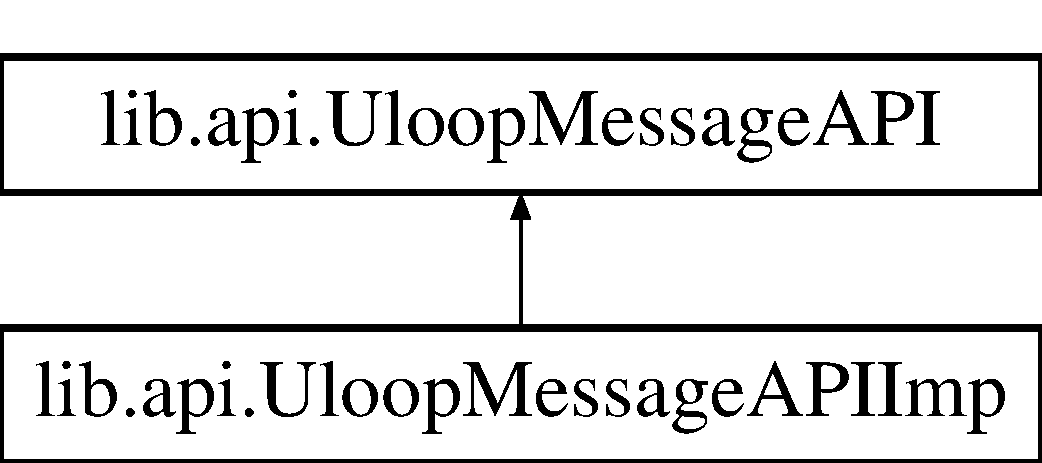
\includegraphics[height=2.000000cm]{classlib_1_1api_1_1UloopMessageAPIImp}
\end{center}
\end{figure}
\subsection*{Public Member Functions}
\begin{DoxyCompactItemize}
\item 
\hyperlink{classlib_1_1api_1_1UloopMessageAPIImp_a3838a3ff54de47d665210ec2184fc05b}{Uloop\+Message\+A\+P\+I\+Imp} (Inet\+Socket\+Address address)
\item 
\hyperlink{classlib_1_1api_1_1UloopMessageAPIImp_a48adacb111673693aa50a12f36dd7c48}{Uloop\+Message\+A\+P\+I\+Imp} (Socket \hyperlink{classlib_1_1api_1_1UloopMessageAPIImp_a9a4910679873f368a5101048d7a58697}{s})
\item 
Uloop\+Message \hyperlink{classlib_1_1api_1_1UloopMessageAPIImp_aedb5cf7280f59aa3f60447d67d8dca43}{recv\+\_\+message} ()
\item 
void \hyperlink{classlib_1_1api_1_1UloopMessageAPIImp_adc9aa0916e7369b762406eec312399c2}{send\+\_\+service\+\_\+request} (\hyperlink{classlib_1_1api_1_1UloopService}{Uloop\+Service} ulservice)
\item 
\hyperlink{classlib_1_1api_1_1UloopServiceRequest}{Uloop\+Service\+Request} \hyperlink{classlib_1_1api_1_1UloopMessageAPIImp_a918fe9df065241f3e783ac54c605301d}{recv\+\_\+service\+\_\+request} ()
\item 
void \hyperlink{classlib_1_1api_1_1UloopMessageAPIImp_a0e3433dc0fd5bb808c02e9a6a0aacd5b}{send\+\_\+service\+\_\+reply} (\hyperlink{classlib_1_1api_1_1UloopService}{Uloop\+Service} ulservice)
\item 
\hyperlink{classlib_1_1api_1_1UloopServiceReply}{Uloop\+Service\+Reply} \hyperlink{classlib_1_1api_1_1UloopMessageAPIImp_aaa61e6ce7c0251ed1fc6b0419eaf7be5}{recv\+\_\+service\+\_\+reply} ()
\item 
void \hyperlink{classlib_1_1api_1_1UloopMessageAPIImp_a589278b172d0d5c26198311faea04ff2}{send\+\_\+mtracker\+\_\+message} (\hyperlink{classlib_1_1api_1_1UloopMTracker}{Uloop\+M\+Tracker} ulmr)
\item 
\hyperlink{classlib_1_1api_1_1UloopMTracker}{Uloop\+M\+Tracker} \hyperlink{classlib_1_1api_1_1UloopMessageAPIImp_a374e184c88066fedddb8e49c55ce308c}{recv\+\_\+mtracker\+\_\+message} ()
\item 
void \hyperlink{classlib_1_1api_1_1UloopMessageAPIImp_af7ec5f2c6b544c327fb66c4e2c471dbe}{send\+\_\+service\+\_\+update} (\hyperlink{classlib_1_1api_1_1UloopService}{Uloop\+Service} ulservice)
\item 
\hyperlink{classlib_1_1api_1_1UloopService}{Uloop\+Service} \hyperlink{classlib_1_1api_1_1UloopMessageAPIImp_a42681424df55773d662182f95cbb0182}{recv\+\_\+service\+\_\+update} ()
\end{DoxyCompactItemize}
\subsection*{Protected Attributes}
\begin{DoxyCompactItemize}
\item 
Socket \hyperlink{classlib_1_1api_1_1UloopMessageAPIImp_a9a4910679873f368a5101048d7a58697}{s}
\end{DoxyCompactItemize}
\subsection*{Private Member Functions}
\begin{DoxyCompactItemize}
\item 
void \hyperlink{classlib_1_1api_1_1UloopMessageAPIImp_a63350d7e3ca2be3d790ca58edd986cfa}{send\+\_\+data} (Uloop\+Message ulm)
\end{DoxyCompactItemize}


\subsection{Constructor \& Destructor Documentation}
\hypertarget{classlib_1_1api_1_1UloopMessageAPIImp_a3838a3ff54de47d665210ec2184fc05b}{\index{lib\+::api\+::\+Uloop\+Message\+A\+P\+I\+Imp@{lib\+::api\+::\+Uloop\+Message\+A\+P\+I\+Imp}!Uloop\+Message\+A\+P\+I\+Imp@{Uloop\+Message\+A\+P\+I\+Imp}}
\index{Uloop\+Message\+A\+P\+I\+Imp@{Uloop\+Message\+A\+P\+I\+Imp}!lib\+::api\+::\+Uloop\+Message\+A\+P\+I\+Imp@{lib\+::api\+::\+Uloop\+Message\+A\+P\+I\+Imp}}
\subsubsection[{Uloop\+Message\+A\+P\+I\+Imp}]{\setlength{\rightskip}{0pt plus 5cm}lib.\+api.\+Uloop\+Message\+A\+P\+I\+Imp.\+Uloop\+Message\+A\+P\+I\+Imp (
\begin{DoxyParamCaption}
\item[{Inet\+Socket\+Address}]{address}
\end{DoxyParamCaption}
)}}\label{classlib_1_1api_1_1UloopMessageAPIImp_a3838a3ff54de47d665210ec2184fc05b}
\hypertarget{classlib_1_1api_1_1UloopMessageAPIImp_a48adacb111673693aa50a12f36dd7c48}{\index{lib\+::api\+::\+Uloop\+Message\+A\+P\+I\+Imp@{lib\+::api\+::\+Uloop\+Message\+A\+P\+I\+Imp}!Uloop\+Message\+A\+P\+I\+Imp@{Uloop\+Message\+A\+P\+I\+Imp}}
\index{Uloop\+Message\+A\+P\+I\+Imp@{Uloop\+Message\+A\+P\+I\+Imp}!lib\+::api\+::\+Uloop\+Message\+A\+P\+I\+Imp@{lib\+::api\+::\+Uloop\+Message\+A\+P\+I\+Imp}}
\subsubsection[{Uloop\+Message\+A\+P\+I\+Imp}]{\setlength{\rightskip}{0pt plus 5cm}lib.\+api.\+Uloop\+Message\+A\+P\+I\+Imp.\+Uloop\+Message\+A\+P\+I\+Imp (
\begin{DoxyParamCaption}
\item[{Socket}]{s}
\end{DoxyParamCaption}
)}}\label{classlib_1_1api_1_1UloopMessageAPIImp_a48adacb111673693aa50a12f36dd7c48}


\subsection{Member Function Documentation}
\hypertarget{classlib_1_1api_1_1UloopMessageAPIImp_aedb5cf7280f59aa3f60447d67d8dca43}{\index{lib\+::api\+::\+Uloop\+Message\+A\+P\+I\+Imp@{lib\+::api\+::\+Uloop\+Message\+A\+P\+I\+Imp}!recv\+\_\+message@{recv\+\_\+message}}
\index{recv\+\_\+message@{recv\+\_\+message}!lib\+::api\+::\+Uloop\+Message\+A\+P\+I\+Imp@{lib\+::api\+::\+Uloop\+Message\+A\+P\+I\+Imp}}
\subsubsection[{recv\+\_\+message}]{\setlength{\rightskip}{0pt plus 5cm}Uloop\+Message lib.\+api.\+Uloop\+Message\+A\+P\+I\+Imp.\+recv\+\_\+message (
\begin{DoxyParamCaption}
{}
\end{DoxyParamCaption}
)}}\label{classlib_1_1api_1_1UloopMessageAPIImp_aedb5cf7280f59aa3f60447d67d8dca43}


Implements \hyperlink{interfacelib_1_1api_1_1UloopMessageAPI_a8dd1f6a62bff709cb8a0ffd63f22415a}{lib.\+api.\+Uloop\+Message\+A\+P\+I}.

\hypertarget{classlib_1_1api_1_1UloopMessageAPIImp_a374e184c88066fedddb8e49c55ce308c}{\index{lib\+::api\+::\+Uloop\+Message\+A\+P\+I\+Imp@{lib\+::api\+::\+Uloop\+Message\+A\+P\+I\+Imp}!recv\+\_\+mtracker\+\_\+message@{recv\+\_\+mtracker\+\_\+message}}
\index{recv\+\_\+mtracker\+\_\+message@{recv\+\_\+mtracker\+\_\+message}!lib\+::api\+::\+Uloop\+Message\+A\+P\+I\+Imp@{lib\+::api\+::\+Uloop\+Message\+A\+P\+I\+Imp}}
\subsubsection[{recv\+\_\+mtracker\+\_\+message}]{\setlength{\rightskip}{0pt plus 5cm}{\bf Uloop\+M\+Tracker} lib.\+api.\+Uloop\+Message\+A\+P\+I\+Imp.\+recv\+\_\+mtracker\+\_\+message (
\begin{DoxyParamCaption}
{}
\end{DoxyParamCaption}
)}}\label{classlib_1_1api_1_1UloopMessageAPIImp_a374e184c88066fedddb8e49c55ce308c}


Implements \hyperlink{interfacelib_1_1api_1_1UloopMessageAPI_aa1e8c5bebf79203984533fb723a01e19}{lib.\+api.\+Uloop\+Message\+A\+P\+I}.

\hypertarget{classlib_1_1api_1_1UloopMessageAPIImp_aaa61e6ce7c0251ed1fc6b0419eaf7be5}{\index{lib\+::api\+::\+Uloop\+Message\+A\+P\+I\+Imp@{lib\+::api\+::\+Uloop\+Message\+A\+P\+I\+Imp}!recv\+\_\+service\+\_\+reply@{recv\+\_\+service\+\_\+reply}}
\index{recv\+\_\+service\+\_\+reply@{recv\+\_\+service\+\_\+reply}!lib\+::api\+::\+Uloop\+Message\+A\+P\+I\+Imp@{lib\+::api\+::\+Uloop\+Message\+A\+P\+I\+Imp}}
\subsubsection[{recv\+\_\+service\+\_\+reply}]{\setlength{\rightskip}{0pt plus 5cm}{\bf Uloop\+Service\+Reply} lib.\+api.\+Uloop\+Message\+A\+P\+I\+Imp.\+recv\+\_\+service\+\_\+reply (
\begin{DoxyParamCaption}
{}
\end{DoxyParamCaption}
)}}\label{classlib_1_1api_1_1UloopMessageAPIImp_aaa61e6ce7c0251ed1fc6b0419eaf7be5}


Implements \hyperlink{interfacelib_1_1api_1_1UloopMessageAPI_a5b3cb0b20ff7d84eaccbe88b83271b4c}{lib.\+api.\+Uloop\+Message\+A\+P\+I}.

\hypertarget{classlib_1_1api_1_1UloopMessageAPIImp_a918fe9df065241f3e783ac54c605301d}{\index{lib\+::api\+::\+Uloop\+Message\+A\+P\+I\+Imp@{lib\+::api\+::\+Uloop\+Message\+A\+P\+I\+Imp}!recv\+\_\+service\+\_\+request@{recv\+\_\+service\+\_\+request}}
\index{recv\+\_\+service\+\_\+request@{recv\+\_\+service\+\_\+request}!lib\+::api\+::\+Uloop\+Message\+A\+P\+I\+Imp@{lib\+::api\+::\+Uloop\+Message\+A\+P\+I\+Imp}}
\subsubsection[{recv\+\_\+service\+\_\+request}]{\setlength{\rightskip}{0pt plus 5cm}{\bf Uloop\+Service\+Request} lib.\+api.\+Uloop\+Message\+A\+P\+I\+Imp.\+recv\+\_\+service\+\_\+request (
\begin{DoxyParamCaption}
{}
\end{DoxyParamCaption}
)}}\label{classlib_1_1api_1_1UloopMessageAPIImp_a918fe9df065241f3e783ac54c605301d}


Implements \hyperlink{interfacelib_1_1api_1_1UloopMessageAPI_a7867cdc90ec092d844190a00546de522}{lib.\+api.\+Uloop\+Message\+A\+P\+I}.

\hypertarget{classlib_1_1api_1_1UloopMessageAPIImp_a42681424df55773d662182f95cbb0182}{\index{lib\+::api\+::\+Uloop\+Message\+A\+P\+I\+Imp@{lib\+::api\+::\+Uloop\+Message\+A\+P\+I\+Imp}!recv\+\_\+service\+\_\+update@{recv\+\_\+service\+\_\+update}}
\index{recv\+\_\+service\+\_\+update@{recv\+\_\+service\+\_\+update}!lib\+::api\+::\+Uloop\+Message\+A\+P\+I\+Imp@{lib\+::api\+::\+Uloop\+Message\+A\+P\+I\+Imp}}
\subsubsection[{recv\+\_\+service\+\_\+update}]{\setlength{\rightskip}{0pt plus 5cm}{\bf Uloop\+Service} lib.\+api.\+Uloop\+Message\+A\+P\+I\+Imp.\+recv\+\_\+service\+\_\+update (
\begin{DoxyParamCaption}
{}
\end{DoxyParamCaption}
)}}\label{classlib_1_1api_1_1UloopMessageAPIImp_a42681424df55773d662182f95cbb0182}


Implements \hyperlink{interfacelib_1_1api_1_1UloopMessageAPI_add962f0753657aa31556e0646f153ad6}{lib.\+api.\+Uloop\+Message\+A\+P\+I}.

\hypertarget{classlib_1_1api_1_1UloopMessageAPIImp_a63350d7e3ca2be3d790ca58edd986cfa}{\index{lib\+::api\+::\+Uloop\+Message\+A\+P\+I\+Imp@{lib\+::api\+::\+Uloop\+Message\+A\+P\+I\+Imp}!send\+\_\+data@{send\+\_\+data}}
\index{send\+\_\+data@{send\+\_\+data}!lib\+::api\+::\+Uloop\+Message\+A\+P\+I\+Imp@{lib\+::api\+::\+Uloop\+Message\+A\+P\+I\+Imp}}
\subsubsection[{send\+\_\+data}]{\setlength{\rightskip}{0pt plus 5cm}void lib.\+api.\+Uloop\+Message\+A\+P\+I\+Imp.\+send\+\_\+data (
\begin{DoxyParamCaption}
\item[{Uloop\+Message}]{ulm}
\end{DoxyParamCaption}
)\hspace{0.3cm}{\ttfamily [private]}}}\label{classlib_1_1api_1_1UloopMessageAPIImp_a63350d7e3ca2be3d790ca58edd986cfa}
\hypertarget{classlib_1_1api_1_1UloopMessageAPIImp_a589278b172d0d5c26198311faea04ff2}{\index{lib\+::api\+::\+Uloop\+Message\+A\+P\+I\+Imp@{lib\+::api\+::\+Uloop\+Message\+A\+P\+I\+Imp}!send\+\_\+mtracker\+\_\+message@{send\+\_\+mtracker\+\_\+message}}
\index{send\+\_\+mtracker\+\_\+message@{send\+\_\+mtracker\+\_\+message}!lib\+::api\+::\+Uloop\+Message\+A\+P\+I\+Imp@{lib\+::api\+::\+Uloop\+Message\+A\+P\+I\+Imp}}
\subsubsection[{send\+\_\+mtracker\+\_\+message}]{\setlength{\rightskip}{0pt plus 5cm}void lib.\+api.\+Uloop\+Message\+A\+P\+I\+Imp.\+send\+\_\+mtracker\+\_\+message (
\begin{DoxyParamCaption}
\item[{{\bf Uloop\+M\+Tracker}}]{ulmr}
\end{DoxyParamCaption}
)}}\label{classlib_1_1api_1_1UloopMessageAPIImp_a589278b172d0d5c26198311faea04ff2}


Implements \hyperlink{interfacelib_1_1api_1_1UloopMessageAPI_a2d2dfb697a4b02117b056665cc0c0c3d}{lib.\+api.\+Uloop\+Message\+A\+P\+I}.

\hypertarget{classlib_1_1api_1_1UloopMessageAPIImp_a0e3433dc0fd5bb808c02e9a6a0aacd5b}{\index{lib\+::api\+::\+Uloop\+Message\+A\+P\+I\+Imp@{lib\+::api\+::\+Uloop\+Message\+A\+P\+I\+Imp}!send\+\_\+service\+\_\+reply@{send\+\_\+service\+\_\+reply}}
\index{send\+\_\+service\+\_\+reply@{send\+\_\+service\+\_\+reply}!lib\+::api\+::\+Uloop\+Message\+A\+P\+I\+Imp@{lib\+::api\+::\+Uloop\+Message\+A\+P\+I\+Imp}}
\subsubsection[{send\+\_\+service\+\_\+reply}]{\setlength{\rightskip}{0pt plus 5cm}void lib.\+api.\+Uloop\+Message\+A\+P\+I\+Imp.\+send\+\_\+service\+\_\+reply (
\begin{DoxyParamCaption}
\item[{{\bf Uloop\+Service}}]{ulservice}
\end{DoxyParamCaption}
)}}\label{classlib_1_1api_1_1UloopMessageAPIImp_a0e3433dc0fd5bb808c02e9a6a0aacd5b}


Implements \hyperlink{interfacelib_1_1api_1_1UloopMessageAPI_a1d2c724d79a4840d2c09f108b23b19cd}{lib.\+api.\+Uloop\+Message\+A\+P\+I}.

\hypertarget{classlib_1_1api_1_1UloopMessageAPIImp_adc9aa0916e7369b762406eec312399c2}{\index{lib\+::api\+::\+Uloop\+Message\+A\+P\+I\+Imp@{lib\+::api\+::\+Uloop\+Message\+A\+P\+I\+Imp}!send\+\_\+service\+\_\+request@{send\+\_\+service\+\_\+request}}
\index{send\+\_\+service\+\_\+request@{send\+\_\+service\+\_\+request}!lib\+::api\+::\+Uloop\+Message\+A\+P\+I\+Imp@{lib\+::api\+::\+Uloop\+Message\+A\+P\+I\+Imp}}
\subsubsection[{send\+\_\+service\+\_\+request}]{\setlength{\rightskip}{0pt plus 5cm}void lib.\+api.\+Uloop\+Message\+A\+P\+I\+Imp.\+send\+\_\+service\+\_\+request (
\begin{DoxyParamCaption}
\item[{{\bf Uloop\+Service}}]{ulservice}
\end{DoxyParamCaption}
)}}\label{classlib_1_1api_1_1UloopMessageAPIImp_adc9aa0916e7369b762406eec312399c2}


Implements \hyperlink{interfacelib_1_1api_1_1UloopMessageAPI_a026a74704c323ac8fce79bd9db7084a6}{lib.\+api.\+Uloop\+Message\+A\+P\+I}.

\hypertarget{classlib_1_1api_1_1UloopMessageAPIImp_af7ec5f2c6b544c327fb66c4e2c471dbe}{\index{lib\+::api\+::\+Uloop\+Message\+A\+P\+I\+Imp@{lib\+::api\+::\+Uloop\+Message\+A\+P\+I\+Imp}!send\+\_\+service\+\_\+update@{send\+\_\+service\+\_\+update}}
\index{send\+\_\+service\+\_\+update@{send\+\_\+service\+\_\+update}!lib\+::api\+::\+Uloop\+Message\+A\+P\+I\+Imp@{lib\+::api\+::\+Uloop\+Message\+A\+P\+I\+Imp}}
\subsubsection[{send\+\_\+service\+\_\+update}]{\setlength{\rightskip}{0pt plus 5cm}void lib.\+api.\+Uloop\+Message\+A\+P\+I\+Imp.\+send\+\_\+service\+\_\+update (
\begin{DoxyParamCaption}
\item[{{\bf Uloop\+Service}}]{ulservice}
\end{DoxyParamCaption}
)}}\label{classlib_1_1api_1_1UloopMessageAPIImp_af7ec5f2c6b544c327fb66c4e2c471dbe}


Implements \hyperlink{interfacelib_1_1api_1_1UloopMessageAPI_ad39bbf025b74e84cc9f09f92e52eda45}{lib.\+api.\+Uloop\+Message\+A\+P\+I}.



\subsection{Member Data Documentation}
\hypertarget{classlib_1_1api_1_1UloopMessageAPIImp_a9a4910679873f368a5101048d7a58697}{\index{lib\+::api\+::\+Uloop\+Message\+A\+P\+I\+Imp@{lib\+::api\+::\+Uloop\+Message\+A\+P\+I\+Imp}!s@{s}}
\index{s@{s}!lib\+::api\+::\+Uloop\+Message\+A\+P\+I\+Imp@{lib\+::api\+::\+Uloop\+Message\+A\+P\+I\+Imp}}
\subsubsection[{s}]{\setlength{\rightskip}{0pt plus 5cm}Socket lib.\+api.\+Uloop\+Message\+A\+P\+I\+Imp.\+s\hspace{0.3cm}{\ttfamily [protected]}}}\label{classlib_1_1api_1_1UloopMessageAPIImp_a9a4910679873f368a5101048d7a58697}


The documentation for this class was generated from the following file\+:\begin{DoxyCompactItemize}
\item 
src/lib/api/\hyperlink{UloopMessageAPIImp_8java}{Uloop\+Message\+A\+P\+I\+Imp.\+java}\end{DoxyCompactItemize}

\hypertarget{interfaceeu_1_1uloop_1_1messages_1_1UloopMessages_1_1UloopMessageOrBuilder}{\section{eu.\+uloop.\+messages.\+Uloop\+Messages.\+Uloop\+Message\+Or\+Builder Interface Reference}
\label{interfaceeu_1_1uloop_1_1messages_1_1UloopMessages_1_1UloopMessageOrBuilder}\index{eu.\+uloop.\+messages.\+Uloop\+Messages.\+Uloop\+Message\+Or\+Builder@{eu.\+uloop.\+messages.\+Uloop\+Messages.\+Uloop\+Message\+Or\+Builder}}
}
Inheritance diagram for eu.\+uloop.\+messages.\+Uloop\+Messages.\+Uloop\+Message\+Or\+Builder\+:\begin{figure}[H]
\begin{center}
\leavevmode
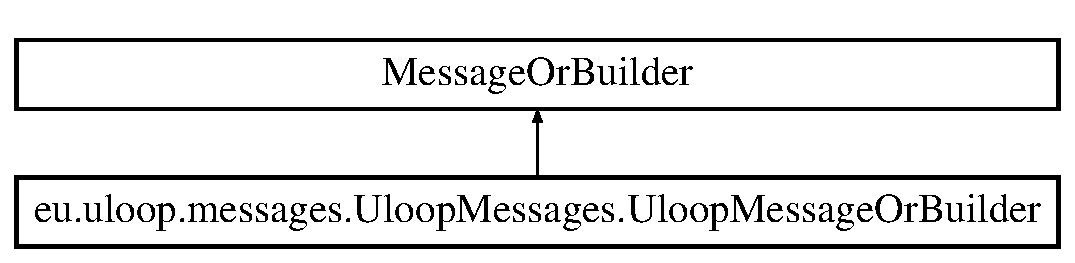
\includegraphics[height=2.000000cm]{interfaceeu_1_1uloop_1_1messages_1_1UloopMessages_1_1UloopMessageOrBuilder}
\end{center}
\end{figure}
\subsection*{Public Member Functions}
\begin{DoxyCompactItemize}
\item 
boolean \hyperlink{interfaceeu_1_1uloop_1_1messages_1_1UloopMessages_1_1UloopMessageOrBuilder_a15bc6942f889d7543772724e1ba252b9}{has\+Tm} ()
\item 
eu.\+uloop.\+messages.\+Uloop\+Messages.\+Trust\+Message \hyperlink{interfaceeu_1_1uloop_1_1messages_1_1UloopMessages_1_1UloopMessageOrBuilder_a5f9e7de3e0cc0ccefce160b62617083c}{get\+Tm} ()
\item 
\hyperlink{interfaceeu_1_1uloop_1_1messages_1_1UloopMessages_1_1TrustMessageOrBuilder}{eu.\+uloop.\+messages.\+Uloop\+Messages.\+Trust\+Message\+Or\+Builder} \hyperlink{interfaceeu_1_1uloop_1_1messages_1_1UloopMessages_1_1UloopMessageOrBuilder_a89debc14c7c00e06032231ddf0b50f28}{get\+Tm\+Or\+Builder} ()
\item 
boolean \hyperlink{interfaceeu_1_1uloop_1_1messages_1_1UloopMessages_1_1UloopMessageOrBuilder_ac122222acf94b2f06f9b4398f8278235}{has\+Rm} ()
\item 
eu.\+uloop.\+messages.\+Uloop\+Messages.\+Resource\+Message \hyperlink{interfaceeu_1_1uloop_1_1messages_1_1UloopMessages_1_1UloopMessageOrBuilder_a802371fb439d609f1e62a8b05205fdff}{get\+Rm} ()
\item 
\hyperlink{interfaceeu_1_1uloop_1_1messages_1_1UloopMessages_1_1ResourceMessageOrBuilder}{eu.\+uloop.\+messages.\+Uloop\+Messages.\+Resource\+Message\+Or\+Builder} \hyperlink{interfaceeu_1_1uloop_1_1messages_1_1UloopMessages_1_1UloopMessageOrBuilder_a2e24f0e2fed84a8a367884af83898b2e}{get\+Rm\+Or\+Builder} ()
\item 
boolean \hyperlink{interfaceeu_1_1uloop_1_1messages_1_1UloopMessages_1_1UloopMessageOrBuilder_af639135351f0506feafaeec8790b1cf5}{has\+Nsm} ()
\item 
eu.\+uloop.\+messages.\+Uloop\+Messages.\+Network\+Status\+Message \hyperlink{interfaceeu_1_1uloop_1_1messages_1_1UloopMessages_1_1UloopMessageOrBuilder_a143ae0fd01a45c24c31094abf9b89ccc}{get\+Nsm} ()
\item 
\hyperlink{interfaceeu_1_1uloop_1_1messages_1_1UloopMessages_1_1NetworkStatusMessageOrBuilder}{eu.\+uloop.\+messages.\+Uloop\+Messages.\+Network\+Status\+Message\+Or\+Builder} \hyperlink{interfaceeu_1_1uloop_1_1messages_1_1UloopMessages_1_1UloopMessageOrBuilder_a806ba3ee27017599e08eae34c7f59f59}{get\+Nsm\+Or\+Builder} ()
\item 
boolean \hyperlink{interfaceeu_1_1uloop_1_1messages_1_1UloopMessages_1_1UloopMessageOrBuilder_a7e1dc3cd80748e1ea1fbd7c841346836}{has\+Udm} ()
\item 
eu.\+uloop.\+messages.\+Uloop\+Messages.\+New\+User\+Details\+Message \hyperlink{interfaceeu_1_1uloop_1_1messages_1_1UloopMessages_1_1UloopMessageOrBuilder_a7cfe01ecc1f958372b9424d78c56839d}{get\+Udm} ()
\item 
\hyperlink{interfaceeu_1_1uloop_1_1messages_1_1UloopMessages_1_1NewUserDetailsMessageOrBuilder}{eu.\+uloop.\+messages.\+Uloop\+Messages.\+New\+User\+Details\+Message\+Or\+Builder} \hyperlink{interfaceeu_1_1uloop_1_1messages_1_1UloopMessages_1_1UloopMessageOrBuilder_ab9ee2e91682ec0b251b2a9b39f1601a7}{get\+Udm\+Or\+Builder} ()
\item 
boolean \hyperlink{interfaceeu_1_1uloop_1_1messages_1_1UloopMessages_1_1UloopMessageOrBuilder_ac245b297ccf051ed50b3304550361b41}{has\+Qos} ()
\item 
eu.\+uloop.\+messages.\+Uloop\+Messages.\+Qo\+S\+Message \hyperlink{interfaceeu_1_1uloop_1_1messages_1_1UloopMessages_1_1UloopMessageOrBuilder_acaf90a5ad44ca054d2029990ef67c7ac}{get\+Qos} ()
\item 
\hyperlink{interfaceeu_1_1uloop_1_1messages_1_1UloopMessages_1_1QoSMessageOrBuilder}{eu.\+uloop.\+messages.\+Uloop\+Messages.\+Qo\+S\+Message\+Or\+Builder} \hyperlink{interfaceeu_1_1uloop_1_1messages_1_1UloopMessages_1_1UloopMessageOrBuilder_a7616dc3de5ac47dd894c53b41302cf50}{get\+Qos\+Or\+Builder} ()
\item 
boolean \hyperlink{interfaceeu_1_1uloop_1_1messages_1_1UloopMessages_1_1UloopMessageOrBuilder_ae218efc11084c2431c8a4c8738f27260}{has\+Ult} ()
\item 
\hyperlink{enumeu_1_1uloop_1_1messages_1_1UloopMessages_1_1UloopMessageType}{eu.\+uloop.\+messages.\+Uloop\+Messages.\+Uloop\+Message\+Type} \hyperlink{interfaceeu_1_1uloop_1_1messages_1_1UloopMessages_1_1UloopMessageOrBuilder_a89717649b52c2ce548c877996b18285d}{get\+Ult} ()
\item 
boolean \hyperlink{interfaceeu_1_1uloop_1_1messages_1_1UloopMessages_1_1UloopMessageOrBuilder_a9ee576bb30591dbca47532391205d40d}{has\+Servm} ()
\item 
eu.\+uloop.\+messages.\+Uloop\+Messages.\+Service\+Message \hyperlink{interfaceeu_1_1uloop_1_1messages_1_1UloopMessages_1_1UloopMessageOrBuilder_aa484b765e04b381b9aed5a4eee679fc8}{get\+Servm} ()
\item 
\hyperlink{interfaceeu_1_1uloop_1_1messages_1_1UloopMessages_1_1ServiceMessageOrBuilder}{eu.\+uloop.\+messages.\+Uloop\+Messages.\+Service\+Message\+Or\+Builder} \hyperlink{interfaceeu_1_1uloop_1_1messages_1_1UloopMessages_1_1UloopMessageOrBuilder_a2543acfdff88bf3c55e41a2747bf3acf}{get\+Servm\+Or\+Builder} ()
\item 
boolean \hyperlink{interfaceeu_1_1uloop_1_1messages_1_1UloopMessages_1_1UloopMessageOrBuilder_a3624829947d38b05a5230feb5cc92a9e}{has\+Mtracker} ()
\item 
eu.\+uloop.\+messages.\+Uloop\+Messages.\+M\+Tracker\+Message \hyperlink{interfaceeu_1_1uloop_1_1messages_1_1UloopMessages_1_1UloopMessageOrBuilder_a53f9bc39fd721b8fd7b1cdd22e76f3e7}{get\+Mtracker} ()
\item 
\hyperlink{interfaceeu_1_1uloop_1_1messages_1_1UloopMessages_1_1MTrackerMessageOrBuilder}{eu.\+uloop.\+messages.\+Uloop\+Messages.\+M\+Tracker\+Message\+Or\+Builder} \hyperlink{interfaceeu_1_1uloop_1_1messages_1_1UloopMessages_1_1UloopMessageOrBuilder_a07420470bdc38be00cddbf74b435b502}{get\+Mtracker\+Or\+Builder} ()
\end{DoxyCompactItemize}


\subsection{Member Function Documentation}
\hypertarget{interfaceeu_1_1uloop_1_1messages_1_1UloopMessages_1_1UloopMessageOrBuilder_a53f9bc39fd721b8fd7b1cdd22e76f3e7}{\index{eu\+::uloop\+::messages\+::\+Uloop\+Messages\+::\+Uloop\+Message\+Or\+Builder@{eu\+::uloop\+::messages\+::\+Uloop\+Messages\+::\+Uloop\+Message\+Or\+Builder}!get\+Mtracker@{get\+Mtracker}}
\index{get\+Mtracker@{get\+Mtracker}!eu\+::uloop\+::messages\+::\+Uloop\+Messages\+::\+Uloop\+Message\+Or\+Builder@{eu\+::uloop\+::messages\+::\+Uloop\+Messages\+::\+Uloop\+Message\+Or\+Builder}}
\subsubsection[{get\+Mtracker}]{\setlength{\rightskip}{0pt plus 5cm}eu.\+uloop.\+messages.\+Uloop\+Messages.\+M\+Tracker\+Message eu.\+uloop.\+messages.\+Uloop\+Messages.\+Uloop\+Message\+Or\+Builder.\+get\+Mtracker (
\begin{DoxyParamCaption}
{}
\end{DoxyParamCaption}
)}}\label{interfaceeu_1_1uloop_1_1messages_1_1UloopMessages_1_1UloopMessageOrBuilder_a53f9bc39fd721b8fd7b1cdd22e76f3e7}
\hypertarget{interfaceeu_1_1uloop_1_1messages_1_1UloopMessages_1_1UloopMessageOrBuilder_a07420470bdc38be00cddbf74b435b502}{\index{eu\+::uloop\+::messages\+::\+Uloop\+Messages\+::\+Uloop\+Message\+Or\+Builder@{eu\+::uloop\+::messages\+::\+Uloop\+Messages\+::\+Uloop\+Message\+Or\+Builder}!get\+Mtracker\+Or\+Builder@{get\+Mtracker\+Or\+Builder}}
\index{get\+Mtracker\+Or\+Builder@{get\+Mtracker\+Or\+Builder}!eu\+::uloop\+::messages\+::\+Uloop\+Messages\+::\+Uloop\+Message\+Or\+Builder@{eu\+::uloop\+::messages\+::\+Uloop\+Messages\+::\+Uloop\+Message\+Or\+Builder}}
\subsubsection[{get\+Mtracker\+Or\+Builder}]{\setlength{\rightskip}{0pt plus 5cm}{\bf eu.\+uloop.\+messages.\+Uloop\+Messages.\+M\+Tracker\+Message\+Or\+Builder} eu.\+uloop.\+messages.\+Uloop\+Messages.\+Uloop\+Message\+Or\+Builder.\+get\+Mtracker\+Or\+Builder (
\begin{DoxyParamCaption}
{}
\end{DoxyParamCaption}
)}}\label{interfaceeu_1_1uloop_1_1messages_1_1UloopMessages_1_1UloopMessageOrBuilder_a07420470bdc38be00cddbf74b435b502}
\hypertarget{interfaceeu_1_1uloop_1_1messages_1_1UloopMessages_1_1UloopMessageOrBuilder_a143ae0fd01a45c24c31094abf9b89ccc}{\index{eu\+::uloop\+::messages\+::\+Uloop\+Messages\+::\+Uloop\+Message\+Or\+Builder@{eu\+::uloop\+::messages\+::\+Uloop\+Messages\+::\+Uloop\+Message\+Or\+Builder}!get\+Nsm@{get\+Nsm}}
\index{get\+Nsm@{get\+Nsm}!eu\+::uloop\+::messages\+::\+Uloop\+Messages\+::\+Uloop\+Message\+Or\+Builder@{eu\+::uloop\+::messages\+::\+Uloop\+Messages\+::\+Uloop\+Message\+Or\+Builder}}
\subsubsection[{get\+Nsm}]{\setlength{\rightskip}{0pt plus 5cm}eu.\+uloop.\+messages.\+Uloop\+Messages.\+Network\+Status\+Message eu.\+uloop.\+messages.\+Uloop\+Messages.\+Uloop\+Message\+Or\+Builder.\+get\+Nsm (
\begin{DoxyParamCaption}
{}
\end{DoxyParamCaption}
)}}\label{interfaceeu_1_1uloop_1_1messages_1_1UloopMessages_1_1UloopMessageOrBuilder_a143ae0fd01a45c24c31094abf9b89ccc}
\hypertarget{interfaceeu_1_1uloop_1_1messages_1_1UloopMessages_1_1UloopMessageOrBuilder_a806ba3ee27017599e08eae34c7f59f59}{\index{eu\+::uloop\+::messages\+::\+Uloop\+Messages\+::\+Uloop\+Message\+Or\+Builder@{eu\+::uloop\+::messages\+::\+Uloop\+Messages\+::\+Uloop\+Message\+Or\+Builder}!get\+Nsm\+Or\+Builder@{get\+Nsm\+Or\+Builder}}
\index{get\+Nsm\+Or\+Builder@{get\+Nsm\+Or\+Builder}!eu\+::uloop\+::messages\+::\+Uloop\+Messages\+::\+Uloop\+Message\+Or\+Builder@{eu\+::uloop\+::messages\+::\+Uloop\+Messages\+::\+Uloop\+Message\+Or\+Builder}}
\subsubsection[{get\+Nsm\+Or\+Builder}]{\setlength{\rightskip}{0pt plus 5cm}{\bf eu.\+uloop.\+messages.\+Uloop\+Messages.\+Network\+Status\+Message\+Or\+Builder} eu.\+uloop.\+messages.\+Uloop\+Messages.\+Uloop\+Message\+Or\+Builder.\+get\+Nsm\+Or\+Builder (
\begin{DoxyParamCaption}
{}
\end{DoxyParamCaption}
)}}\label{interfaceeu_1_1uloop_1_1messages_1_1UloopMessages_1_1UloopMessageOrBuilder_a806ba3ee27017599e08eae34c7f59f59}
\hypertarget{interfaceeu_1_1uloop_1_1messages_1_1UloopMessages_1_1UloopMessageOrBuilder_acaf90a5ad44ca054d2029990ef67c7ac}{\index{eu\+::uloop\+::messages\+::\+Uloop\+Messages\+::\+Uloop\+Message\+Or\+Builder@{eu\+::uloop\+::messages\+::\+Uloop\+Messages\+::\+Uloop\+Message\+Or\+Builder}!get\+Qos@{get\+Qos}}
\index{get\+Qos@{get\+Qos}!eu\+::uloop\+::messages\+::\+Uloop\+Messages\+::\+Uloop\+Message\+Or\+Builder@{eu\+::uloop\+::messages\+::\+Uloop\+Messages\+::\+Uloop\+Message\+Or\+Builder}}
\subsubsection[{get\+Qos}]{\setlength{\rightskip}{0pt plus 5cm}eu.\+uloop.\+messages.\+Uloop\+Messages.\+Qo\+S\+Message eu.\+uloop.\+messages.\+Uloop\+Messages.\+Uloop\+Message\+Or\+Builder.\+get\+Qos (
\begin{DoxyParamCaption}
{}
\end{DoxyParamCaption}
)}}\label{interfaceeu_1_1uloop_1_1messages_1_1UloopMessages_1_1UloopMessageOrBuilder_acaf90a5ad44ca054d2029990ef67c7ac}
\hypertarget{interfaceeu_1_1uloop_1_1messages_1_1UloopMessages_1_1UloopMessageOrBuilder_a7616dc3de5ac47dd894c53b41302cf50}{\index{eu\+::uloop\+::messages\+::\+Uloop\+Messages\+::\+Uloop\+Message\+Or\+Builder@{eu\+::uloop\+::messages\+::\+Uloop\+Messages\+::\+Uloop\+Message\+Or\+Builder}!get\+Qos\+Or\+Builder@{get\+Qos\+Or\+Builder}}
\index{get\+Qos\+Or\+Builder@{get\+Qos\+Or\+Builder}!eu\+::uloop\+::messages\+::\+Uloop\+Messages\+::\+Uloop\+Message\+Or\+Builder@{eu\+::uloop\+::messages\+::\+Uloop\+Messages\+::\+Uloop\+Message\+Or\+Builder}}
\subsubsection[{get\+Qos\+Or\+Builder}]{\setlength{\rightskip}{0pt plus 5cm}{\bf eu.\+uloop.\+messages.\+Uloop\+Messages.\+Qo\+S\+Message\+Or\+Builder} eu.\+uloop.\+messages.\+Uloop\+Messages.\+Uloop\+Message\+Or\+Builder.\+get\+Qos\+Or\+Builder (
\begin{DoxyParamCaption}
{}
\end{DoxyParamCaption}
)}}\label{interfaceeu_1_1uloop_1_1messages_1_1UloopMessages_1_1UloopMessageOrBuilder_a7616dc3de5ac47dd894c53b41302cf50}
\hypertarget{interfaceeu_1_1uloop_1_1messages_1_1UloopMessages_1_1UloopMessageOrBuilder_a802371fb439d609f1e62a8b05205fdff}{\index{eu\+::uloop\+::messages\+::\+Uloop\+Messages\+::\+Uloop\+Message\+Or\+Builder@{eu\+::uloop\+::messages\+::\+Uloop\+Messages\+::\+Uloop\+Message\+Or\+Builder}!get\+Rm@{get\+Rm}}
\index{get\+Rm@{get\+Rm}!eu\+::uloop\+::messages\+::\+Uloop\+Messages\+::\+Uloop\+Message\+Or\+Builder@{eu\+::uloop\+::messages\+::\+Uloop\+Messages\+::\+Uloop\+Message\+Or\+Builder}}
\subsubsection[{get\+Rm}]{\setlength{\rightskip}{0pt plus 5cm}eu.\+uloop.\+messages.\+Uloop\+Messages.\+Resource\+Message eu.\+uloop.\+messages.\+Uloop\+Messages.\+Uloop\+Message\+Or\+Builder.\+get\+Rm (
\begin{DoxyParamCaption}
{}
\end{DoxyParamCaption}
)}}\label{interfaceeu_1_1uloop_1_1messages_1_1UloopMessages_1_1UloopMessageOrBuilder_a802371fb439d609f1e62a8b05205fdff}
\hypertarget{interfaceeu_1_1uloop_1_1messages_1_1UloopMessages_1_1UloopMessageOrBuilder_a2e24f0e2fed84a8a367884af83898b2e}{\index{eu\+::uloop\+::messages\+::\+Uloop\+Messages\+::\+Uloop\+Message\+Or\+Builder@{eu\+::uloop\+::messages\+::\+Uloop\+Messages\+::\+Uloop\+Message\+Or\+Builder}!get\+Rm\+Or\+Builder@{get\+Rm\+Or\+Builder}}
\index{get\+Rm\+Or\+Builder@{get\+Rm\+Or\+Builder}!eu\+::uloop\+::messages\+::\+Uloop\+Messages\+::\+Uloop\+Message\+Or\+Builder@{eu\+::uloop\+::messages\+::\+Uloop\+Messages\+::\+Uloop\+Message\+Or\+Builder}}
\subsubsection[{get\+Rm\+Or\+Builder}]{\setlength{\rightskip}{0pt plus 5cm}{\bf eu.\+uloop.\+messages.\+Uloop\+Messages.\+Resource\+Message\+Or\+Builder} eu.\+uloop.\+messages.\+Uloop\+Messages.\+Uloop\+Message\+Or\+Builder.\+get\+Rm\+Or\+Builder (
\begin{DoxyParamCaption}
{}
\end{DoxyParamCaption}
)}}\label{interfaceeu_1_1uloop_1_1messages_1_1UloopMessages_1_1UloopMessageOrBuilder_a2e24f0e2fed84a8a367884af83898b2e}
\hypertarget{interfaceeu_1_1uloop_1_1messages_1_1UloopMessages_1_1UloopMessageOrBuilder_aa484b765e04b381b9aed5a4eee679fc8}{\index{eu\+::uloop\+::messages\+::\+Uloop\+Messages\+::\+Uloop\+Message\+Or\+Builder@{eu\+::uloop\+::messages\+::\+Uloop\+Messages\+::\+Uloop\+Message\+Or\+Builder}!get\+Servm@{get\+Servm}}
\index{get\+Servm@{get\+Servm}!eu\+::uloop\+::messages\+::\+Uloop\+Messages\+::\+Uloop\+Message\+Or\+Builder@{eu\+::uloop\+::messages\+::\+Uloop\+Messages\+::\+Uloop\+Message\+Or\+Builder}}
\subsubsection[{get\+Servm}]{\setlength{\rightskip}{0pt plus 5cm}eu.\+uloop.\+messages.\+Uloop\+Messages.\+Service\+Message eu.\+uloop.\+messages.\+Uloop\+Messages.\+Uloop\+Message\+Or\+Builder.\+get\+Servm (
\begin{DoxyParamCaption}
{}
\end{DoxyParamCaption}
)}}\label{interfaceeu_1_1uloop_1_1messages_1_1UloopMessages_1_1UloopMessageOrBuilder_aa484b765e04b381b9aed5a4eee679fc8}
\hypertarget{interfaceeu_1_1uloop_1_1messages_1_1UloopMessages_1_1UloopMessageOrBuilder_a2543acfdff88bf3c55e41a2747bf3acf}{\index{eu\+::uloop\+::messages\+::\+Uloop\+Messages\+::\+Uloop\+Message\+Or\+Builder@{eu\+::uloop\+::messages\+::\+Uloop\+Messages\+::\+Uloop\+Message\+Or\+Builder}!get\+Servm\+Or\+Builder@{get\+Servm\+Or\+Builder}}
\index{get\+Servm\+Or\+Builder@{get\+Servm\+Or\+Builder}!eu\+::uloop\+::messages\+::\+Uloop\+Messages\+::\+Uloop\+Message\+Or\+Builder@{eu\+::uloop\+::messages\+::\+Uloop\+Messages\+::\+Uloop\+Message\+Or\+Builder}}
\subsubsection[{get\+Servm\+Or\+Builder}]{\setlength{\rightskip}{0pt plus 5cm}{\bf eu.\+uloop.\+messages.\+Uloop\+Messages.\+Service\+Message\+Or\+Builder} eu.\+uloop.\+messages.\+Uloop\+Messages.\+Uloop\+Message\+Or\+Builder.\+get\+Servm\+Or\+Builder (
\begin{DoxyParamCaption}
{}
\end{DoxyParamCaption}
)}}\label{interfaceeu_1_1uloop_1_1messages_1_1UloopMessages_1_1UloopMessageOrBuilder_a2543acfdff88bf3c55e41a2747bf3acf}
\hypertarget{interfaceeu_1_1uloop_1_1messages_1_1UloopMessages_1_1UloopMessageOrBuilder_a5f9e7de3e0cc0ccefce160b62617083c}{\index{eu\+::uloop\+::messages\+::\+Uloop\+Messages\+::\+Uloop\+Message\+Or\+Builder@{eu\+::uloop\+::messages\+::\+Uloop\+Messages\+::\+Uloop\+Message\+Or\+Builder}!get\+Tm@{get\+Tm}}
\index{get\+Tm@{get\+Tm}!eu\+::uloop\+::messages\+::\+Uloop\+Messages\+::\+Uloop\+Message\+Or\+Builder@{eu\+::uloop\+::messages\+::\+Uloop\+Messages\+::\+Uloop\+Message\+Or\+Builder}}
\subsubsection[{get\+Tm}]{\setlength{\rightskip}{0pt plus 5cm}eu.\+uloop.\+messages.\+Uloop\+Messages.\+Trust\+Message eu.\+uloop.\+messages.\+Uloop\+Messages.\+Uloop\+Message\+Or\+Builder.\+get\+Tm (
\begin{DoxyParamCaption}
{}
\end{DoxyParamCaption}
)}}\label{interfaceeu_1_1uloop_1_1messages_1_1UloopMessages_1_1UloopMessageOrBuilder_a5f9e7de3e0cc0ccefce160b62617083c}
\hypertarget{interfaceeu_1_1uloop_1_1messages_1_1UloopMessages_1_1UloopMessageOrBuilder_a89debc14c7c00e06032231ddf0b50f28}{\index{eu\+::uloop\+::messages\+::\+Uloop\+Messages\+::\+Uloop\+Message\+Or\+Builder@{eu\+::uloop\+::messages\+::\+Uloop\+Messages\+::\+Uloop\+Message\+Or\+Builder}!get\+Tm\+Or\+Builder@{get\+Tm\+Or\+Builder}}
\index{get\+Tm\+Or\+Builder@{get\+Tm\+Or\+Builder}!eu\+::uloop\+::messages\+::\+Uloop\+Messages\+::\+Uloop\+Message\+Or\+Builder@{eu\+::uloop\+::messages\+::\+Uloop\+Messages\+::\+Uloop\+Message\+Or\+Builder}}
\subsubsection[{get\+Tm\+Or\+Builder}]{\setlength{\rightskip}{0pt plus 5cm}{\bf eu.\+uloop.\+messages.\+Uloop\+Messages.\+Trust\+Message\+Or\+Builder} eu.\+uloop.\+messages.\+Uloop\+Messages.\+Uloop\+Message\+Or\+Builder.\+get\+Tm\+Or\+Builder (
\begin{DoxyParamCaption}
{}
\end{DoxyParamCaption}
)}}\label{interfaceeu_1_1uloop_1_1messages_1_1UloopMessages_1_1UloopMessageOrBuilder_a89debc14c7c00e06032231ddf0b50f28}
\hypertarget{interfaceeu_1_1uloop_1_1messages_1_1UloopMessages_1_1UloopMessageOrBuilder_a7cfe01ecc1f958372b9424d78c56839d}{\index{eu\+::uloop\+::messages\+::\+Uloop\+Messages\+::\+Uloop\+Message\+Or\+Builder@{eu\+::uloop\+::messages\+::\+Uloop\+Messages\+::\+Uloop\+Message\+Or\+Builder}!get\+Udm@{get\+Udm}}
\index{get\+Udm@{get\+Udm}!eu\+::uloop\+::messages\+::\+Uloop\+Messages\+::\+Uloop\+Message\+Or\+Builder@{eu\+::uloop\+::messages\+::\+Uloop\+Messages\+::\+Uloop\+Message\+Or\+Builder}}
\subsubsection[{get\+Udm}]{\setlength{\rightskip}{0pt plus 5cm}eu.\+uloop.\+messages.\+Uloop\+Messages.\+New\+User\+Details\+Message eu.\+uloop.\+messages.\+Uloop\+Messages.\+Uloop\+Message\+Or\+Builder.\+get\+Udm (
\begin{DoxyParamCaption}
{}
\end{DoxyParamCaption}
)}}\label{interfaceeu_1_1uloop_1_1messages_1_1UloopMessages_1_1UloopMessageOrBuilder_a7cfe01ecc1f958372b9424d78c56839d}
\hypertarget{interfaceeu_1_1uloop_1_1messages_1_1UloopMessages_1_1UloopMessageOrBuilder_ab9ee2e91682ec0b251b2a9b39f1601a7}{\index{eu\+::uloop\+::messages\+::\+Uloop\+Messages\+::\+Uloop\+Message\+Or\+Builder@{eu\+::uloop\+::messages\+::\+Uloop\+Messages\+::\+Uloop\+Message\+Or\+Builder}!get\+Udm\+Or\+Builder@{get\+Udm\+Or\+Builder}}
\index{get\+Udm\+Or\+Builder@{get\+Udm\+Or\+Builder}!eu\+::uloop\+::messages\+::\+Uloop\+Messages\+::\+Uloop\+Message\+Or\+Builder@{eu\+::uloop\+::messages\+::\+Uloop\+Messages\+::\+Uloop\+Message\+Or\+Builder}}
\subsubsection[{get\+Udm\+Or\+Builder}]{\setlength{\rightskip}{0pt plus 5cm}{\bf eu.\+uloop.\+messages.\+Uloop\+Messages.\+New\+User\+Details\+Message\+Or\+Builder} eu.\+uloop.\+messages.\+Uloop\+Messages.\+Uloop\+Message\+Or\+Builder.\+get\+Udm\+Or\+Builder (
\begin{DoxyParamCaption}
{}
\end{DoxyParamCaption}
)}}\label{interfaceeu_1_1uloop_1_1messages_1_1UloopMessages_1_1UloopMessageOrBuilder_ab9ee2e91682ec0b251b2a9b39f1601a7}
\hypertarget{interfaceeu_1_1uloop_1_1messages_1_1UloopMessages_1_1UloopMessageOrBuilder_a89717649b52c2ce548c877996b18285d}{\index{eu\+::uloop\+::messages\+::\+Uloop\+Messages\+::\+Uloop\+Message\+Or\+Builder@{eu\+::uloop\+::messages\+::\+Uloop\+Messages\+::\+Uloop\+Message\+Or\+Builder}!get\+Ult@{get\+Ult}}
\index{get\+Ult@{get\+Ult}!eu\+::uloop\+::messages\+::\+Uloop\+Messages\+::\+Uloop\+Message\+Or\+Builder@{eu\+::uloop\+::messages\+::\+Uloop\+Messages\+::\+Uloop\+Message\+Or\+Builder}}
\subsubsection[{get\+Ult}]{\setlength{\rightskip}{0pt plus 5cm}{\bf eu.\+uloop.\+messages.\+Uloop\+Messages.\+Uloop\+Message\+Type} eu.\+uloop.\+messages.\+Uloop\+Messages.\+Uloop\+Message\+Or\+Builder.\+get\+Ult (
\begin{DoxyParamCaption}
{}
\end{DoxyParamCaption}
)}}\label{interfaceeu_1_1uloop_1_1messages_1_1UloopMessages_1_1UloopMessageOrBuilder_a89717649b52c2ce548c877996b18285d}
\hypertarget{interfaceeu_1_1uloop_1_1messages_1_1UloopMessages_1_1UloopMessageOrBuilder_a3624829947d38b05a5230feb5cc92a9e}{\index{eu\+::uloop\+::messages\+::\+Uloop\+Messages\+::\+Uloop\+Message\+Or\+Builder@{eu\+::uloop\+::messages\+::\+Uloop\+Messages\+::\+Uloop\+Message\+Or\+Builder}!has\+Mtracker@{has\+Mtracker}}
\index{has\+Mtracker@{has\+Mtracker}!eu\+::uloop\+::messages\+::\+Uloop\+Messages\+::\+Uloop\+Message\+Or\+Builder@{eu\+::uloop\+::messages\+::\+Uloop\+Messages\+::\+Uloop\+Message\+Or\+Builder}}
\subsubsection[{has\+Mtracker}]{\setlength{\rightskip}{0pt plus 5cm}boolean eu.\+uloop.\+messages.\+Uloop\+Messages.\+Uloop\+Message\+Or\+Builder.\+has\+Mtracker (
\begin{DoxyParamCaption}
{}
\end{DoxyParamCaption}
)}}\label{interfaceeu_1_1uloop_1_1messages_1_1UloopMessages_1_1UloopMessageOrBuilder_a3624829947d38b05a5230feb5cc92a9e}
\hypertarget{interfaceeu_1_1uloop_1_1messages_1_1UloopMessages_1_1UloopMessageOrBuilder_af639135351f0506feafaeec8790b1cf5}{\index{eu\+::uloop\+::messages\+::\+Uloop\+Messages\+::\+Uloop\+Message\+Or\+Builder@{eu\+::uloop\+::messages\+::\+Uloop\+Messages\+::\+Uloop\+Message\+Or\+Builder}!has\+Nsm@{has\+Nsm}}
\index{has\+Nsm@{has\+Nsm}!eu\+::uloop\+::messages\+::\+Uloop\+Messages\+::\+Uloop\+Message\+Or\+Builder@{eu\+::uloop\+::messages\+::\+Uloop\+Messages\+::\+Uloop\+Message\+Or\+Builder}}
\subsubsection[{has\+Nsm}]{\setlength{\rightskip}{0pt plus 5cm}boolean eu.\+uloop.\+messages.\+Uloop\+Messages.\+Uloop\+Message\+Or\+Builder.\+has\+Nsm (
\begin{DoxyParamCaption}
{}
\end{DoxyParamCaption}
)}}\label{interfaceeu_1_1uloop_1_1messages_1_1UloopMessages_1_1UloopMessageOrBuilder_af639135351f0506feafaeec8790b1cf5}
\hypertarget{interfaceeu_1_1uloop_1_1messages_1_1UloopMessages_1_1UloopMessageOrBuilder_ac245b297ccf051ed50b3304550361b41}{\index{eu\+::uloop\+::messages\+::\+Uloop\+Messages\+::\+Uloop\+Message\+Or\+Builder@{eu\+::uloop\+::messages\+::\+Uloop\+Messages\+::\+Uloop\+Message\+Or\+Builder}!has\+Qos@{has\+Qos}}
\index{has\+Qos@{has\+Qos}!eu\+::uloop\+::messages\+::\+Uloop\+Messages\+::\+Uloop\+Message\+Or\+Builder@{eu\+::uloop\+::messages\+::\+Uloop\+Messages\+::\+Uloop\+Message\+Or\+Builder}}
\subsubsection[{has\+Qos}]{\setlength{\rightskip}{0pt plus 5cm}boolean eu.\+uloop.\+messages.\+Uloop\+Messages.\+Uloop\+Message\+Or\+Builder.\+has\+Qos (
\begin{DoxyParamCaption}
{}
\end{DoxyParamCaption}
)}}\label{interfaceeu_1_1uloop_1_1messages_1_1UloopMessages_1_1UloopMessageOrBuilder_ac245b297ccf051ed50b3304550361b41}
\hypertarget{interfaceeu_1_1uloop_1_1messages_1_1UloopMessages_1_1UloopMessageOrBuilder_ac122222acf94b2f06f9b4398f8278235}{\index{eu\+::uloop\+::messages\+::\+Uloop\+Messages\+::\+Uloop\+Message\+Or\+Builder@{eu\+::uloop\+::messages\+::\+Uloop\+Messages\+::\+Uloop\+Message\+Or\+Builder}!has\+Rm@{has\+Rm}}
\index{has\+Rm@{has\+Rm}!eu\+::uloop\+::messages\+::\+Uloop\+Messages\+::\+Uloop\+Message\+Or\+Builder@{eu\+::uloop\+::messages\+::\+Uloop\+Messages\+::\+Uloop\+Message\+Or\+Builder}}
\subsubsection[{has\+Rm}]{\setlength{\rightskip}{0pt plus 5cm}boolean eu.\+uloop.\+messages.\+Uloop\+Messages.\+Uloop\+Message\+Or\+Builder.\+has\+Rm (
\begin{DoxyParamCaption}
{}
\end{DoxyParamCaption}
)}}\label{interfaceeu_1_1uloop_1_1messages_1_1UloopMessages_1_1UloopMessageOrBuilder_ac122222acf94b2f06f9b4398f8278235}
\hypertarget{interfaceeu_1_1uloop_1_1messages_1_1UloopMessages_1_1UloopMessageOrBuilder_a9ee576bb30591dbca47532391205d40d}{\index{eu\+::uloop\+::messages\+::\+Uloop\+Messages\+::\+Uloop\+Message\+Or\+Builder@{eu\+::uloop\+::messages\+::\+Uloop\+Messages\+::\+Uloop\+Message\+Or\+Builder}!has\+Servm@{has\+Servm}}
\index{has\+Servm@{has\+Servm}!eu\+::uloop\+::messages\+::\+Uloop\+Messages\+::\+Uloop\+Message\+Or\+Builder@{eu\+::uloop\+::messages\+::\+Uloop\+Messages\+::\+Uloop\+Message\+Or\+Builder}}
\subsubsection[{has\+Servm}]{\setlength{\rightskip}{0pt plus 5cm}boolean eu.\+uloop.\+messages.\+Uloop\+Messages.\+Uloop\+Message\+Or\+Builder.\+has\+Servm (
\begin{DoxyParamCaption}
{}
\end{DoxyParamCaption}
)}}\label{interfaceeu_1_1uloop_1_1messages_1_1UloopMessages_1_1UloopMessageOrBuilder_a9ee576bb30591dbca47532391205d40d}
\hypertarget{interfaceeu_1_1uloop_1_1messages_1_1UloopMessages_1_1UloopMessageOrBuilder_a15bc6942f889d7543772724e1ba252b9}{\index{eu\+::uloop\+::messages\+::\+Uloop\+Messages\+::\+Uloop\+Message\+Or\+Builder@{eu\+::uloop\+::messages\+::\+Uloop\+Messages\+::\+Uloop\+Message\+Or\+Builder}!has\+Tm@{has\+Tm}}
\index{has\+Tm@{has\+Tm}!eu\+::uloop\+::messages\+::\+Uloop\+Messages\+::\+Uloop\+Message\+Or\+Builder@{eu\+::uloop\+::messages\+::\+Uloop\+Messages\+::\+Uloop\+Message\+Or\+Builder}}
\subsubsection[{has\+Tm}]{\setlength{\rightskip}{0pt plus 5cm}boolean eu.\+uloop.\+messages.\+Uloop\+Messages.\+Uloop\+Message\+Or\+Builder.\+has\+Tm (
\begin{DoxyParamCaption}
{}
\end{DoxyParamCaption}
)}}\label{interfaceeu_1_1uloop_1_1messages_1_1UloopMessages_1_1UloopMessageOrBuilder_a15bc6942f889d7543772724e1ba252b9}
\hypertarget{interfaceeu_1_1uloop_1_1messages_1_1UloopMessages_1_1UloopMessageOrBuilder_a7e1dc3cd80748e1ea1fbd7c841346836}{\index{eu\+::uloop\+::messages\+::\+Uloop\+Messages\+::\+Uloop\+Message\+Or\+Builder@{eu\+::uloop\+::messages\+::\+Uloop\+Messages\+::\+Uloop\+Message\+Or\+Builder}!has\+Udm@{has\+Udm}}
\index{has\+Udm@{has\+Udm}!eu\+::uloop\+::messages\+::\+Uloop\+Messages\+::\+Uloop\+Message\+Or\+Builder@{eu\+::uloop\+::messages\+::\+Uloop\+Messages\+::\+Uloop\+Message\+Or\+Builder}}
\subsubsection[{has\+Udm}]{\setlength{\rightskip}{0pt plus 5cm}boolean eu.\+uloop.\+messages.\+Uloop\+Messages.\+Uloop\+Message\+Or\+Builder.\+has\+Udm (
\begin{DoxyParamCaption}
{}
\end{DoxyParamCaption}
)}}\label{interfaceeu_1_1uloop_1_1messages_1_1UloopMessages_1_1UloopMessageOrBuilder_a7e1dc3cd80748e1ea1fbd7c841346836}
\hypertarget{interfaceeu_1_1uloop_1_1messages_1_1UloopMessages_1_1UloopMessageOrBuilder_ae218efc11084c2431c8a4c8738f27260}{\index{eu\+::uloop\+::messages\+::\+Uloop\+Messages\+::\+Uloop\+Message\+Or\+Builder@{eu\+::uloop\+::messages\+::\+Uloop\+Messages\+::\+Uloop\+Message\+Or\+Builder}!has\+Ult@{has\+Ult}}
\index{has\+Ult@{has\+Ult}!eu\+::uloop\+::messages\+::\+Uloop\+Messages\+::\+Uloop\+Message\+Or\+Builder@{eu\+::uloop\+::messages\+::\+Uloop\+Messages\+::\+Uloop\+Message\+Or\+Builder}}
\subsubsection[{has\+Ult}]{\setlength{\rightskip}{0pt plus 5cm}boolean eu.\+uloop.\+messages.\+Uloop\+Messages.\+Uloop\+Message\+Or\+Builder.\+has\+Ult (
\begin{DoxyParamCaption}
{}
\end{DoxyParamCaption}
)}}\label{interfaceeu_1_1uloop_1_1messages_1_1UloopMessages_1_1UloopMessageOrBuilder_ae218efc11084c2431c8a4c8738f27260}


The documentation for this interface was generated from the following file\+:\begin{DoxyCompactItemize}
\item 
src/eu/uloop/messages/\hyperlink{UloopMessages_8java}{Uloop\+Messages.\+java}\end{DoxyCompactItemize}

\hypertarget{classeu_1_1uloop_1_1messages_1_1UloopMessages}{\section{eu.\+uloop.\+messages.\+Uloop\+Messages Class Reference}
\label{classeu_1_1uloop_1_1messages_1_1UloopMessages}\index{eu.\+uloop.\+messages.\+Uloop\+Messages@{eu.\+uloop.\+messages.\+Uloop\+Messages}}
}
\subsection*{Classes}
\begin{DoxyCompactItemize}
\item 
class {\bfseries Enough\+Resources\+C\+A\+C\+Reply}
\item 
interface \hyperlink{interfaceeu_1_1uloop_1_1messages_1_1UloopMessages_1_1EnoughResourcesCACReplyOrBuilder}{Enough\+Resources\+C\+A\+C\+Reply\+Or\+Builder}
\item 
class {\bfseries Enough\+Resources\+Message\+Reply}
\item 
interface \hyperlink{interfaceeu_1_1uloop_1_1messages_1_1UloopMessages_1_1EnoughResourcesMessageReplyOrBuilder}{Enough\+Resources\+Message\+Reply\+Or\+Builder}
\item 
class {\bfseries Enough\+Resources\+Message\+Request}
\item 
interface \hyperlink{interfaceeu_1_1uloop_1_1messages_1_1UloopMessages_1_1EnoughResourcesMessageRequestOrBuilder}{Enough\+Resources\+Message\+Request\+Or\+Builder}
\item 
enum \hyperlink{enumeu_1_1uloop_1_1messages_1_1UloopMessages_1_1MessageType}{Message\+Type}
\item 
class {\bfseries M\+Tracker\+Message}
\item 
interface \hyperlink{interfaceeu_1_1uloop_1_1messages_1_1UloopMessages_1_1MTrackerMessageOrBuilder}{M\+Tracker\+Message\+Or\+Builder}
\item 
class {\bfseries M\+Tracker\+Predicted\+Move}
\item 
interface \hyperlink{interfaceeu_1_1uloop_1_1messages_1_1UloopMessages_1_1MTrackerPredictedMoveOrBuilder}{M\+Tracker\+Predicted\+Move\+Or\+Builder}
\item 
class {\bfseries Network\+Status\+Message}
\item 
interface \hyperlink{interfaceeu_1_1uloop_1_1messages_1_1UloopMessages_1_1NetworkStatusMessageOrBuilder}{Network\+Status\+Message\+Or\+Builder}
\item 
class {\bfseries Network\+Status\+Message\+Reply}
\item 
interface \hyperlink{interfaceeu_1_1uloop_1_1messages_1_1UloopMessages_1_1NetworkStatusMessageReplyOrBuilder}{Network\+Status\+Message\+Reply\+Or\+Builder}
\item 
class {\bfseries New\+User\+Details\+Message}
\item 
interface \hyperlink{interfaceeu_1_1uloop_1_1messages_1_1UloopMessages_1_1NewUserDetailsMessageOrBuilder}{New\+User\+Details\+Message\+Or\+Builder}
\item 
class {\bfseries Qo\+S\+Message}
\item 
interface \hyperlink{interfaceeu_1_1uloop_1_1messages_1_1UloopMessages_1_1QoSMessageOrBuilder}{Qo\+S\+Message\+Or\+Builder}
\item 
class {\bfseries Qos\+Request}
\item 
interface \hyperlink{interfaceeu_1_1uloop_1_1messages_1_1UloopMessages_1_1QosRequestOrBuilder}{Qos\+Request\+Or\+Builder}
\item 
class {\bfseries Qo\+S\+Tuple}
\item 
interface \hyperlink{interfaceeu_1_1uloop_1_1messages_1_1UloopMessages_1_1QoSTupleOrBuilder}{Qo\+S\+Tuple\+Or\+Builder}
\item 
class {\bfseries Resource\+Message}
\item 
interface \hyperlink{interfaceeu_1_1uloop_1_1messages_1_1UloopMessages_1_1ResourceMessageOrBuilder}{Resource\+Message\+Or\+Builder}
\item 
class {\bfseries Service\+Message}
\item 
interface \hyperlink{interfaceeu_1_1uloop_1_1messages_1_1UloopMessages_1_1ServiceMessageOrBuilder}{Service\+Message\+Or\+Builder}
\item 
class {\bfseries Service\+Reply}
\item 
interface \hyperlink{interfaceeu_1_1uloop_1_1messages_1_1UloopMessages_1_1ServiceReplyOrBuilder}{Service\+Reply\+Or\+Builder}
\item 
class {\bfseries Service\+Request}
\item 
interface \hyperlink{interfaceeu_1_1uloop_1_1messages_1_1UloopMessages_1_1ServiceRequestOrBuilder}{Service\+Request\+Or\+Builder}
\item 
class {\bfseries Service\+Update}
\item 
interface \hyperlink{interfaceeu_1_1uloop_1_1messages_1_1UloopMessages_1_1ServiceUpdateOrBuilder}{Service\+Update\+Or\+Builder}
\item 
class {\bfseries Trust\+Information\+Reply}
\item 
interface \hyperlink{interfaceeu_1_1uloop_1_1messages_1_1UloopMessages_1_1TrustInformationReplyOrBuilder}{Trust\+Information\+Reply\+Or\+Builder}
\item 
class {\bfseries Trust\+Information\+Request}
\item 
interface \hyperlink{interfaceeu_1_1uloop_1_1messages_1_1UloopMessages_1_1TrustInformationRequestOrBuilder}{Trust\+Information\+Request\+Or\+Builder}
\item 
class {\bfseries Trust\+Message}
\item 
interface \hyperlink{interfaceeu_1_1uloop_1_1messages_1_1UloopMessages_1_1TrustMessageOrBuilder}{Trust\+Message\+Or\+Builder}
\item 
class {\bfseries Uloop\+Header\+Message}
\item 
interface \hyperlink{interfaceeu_1_1uloop_1_1messages_1_1UloopMessages_1_1UloopHeaderMessageOrBuilder}{Uloop\+Header\+Message\+Or\+Builder}
\item 
class {\bfseries Uloop\+Message}
\item 
interface \hyperlink{interfaceeu_1_1uloop_1_1messages_1_1UloopMessages_1_1UloopMessageOrBuilder}{Uloop\+Message\+Or\+Builder}
\item 
enum \hyperlink{enumeu_1_1uloop_1_1messages_1_1UloopMessages_1_1UloopMessageType}{Uloop\+Message\+Type}
\end{DoxyCompactItemize}
\subsection*{Static Public Member Functions}
\begin{DoxyCompactItemize}
\item 
static void \hyperlink{classeu_1_1uloop_1_1messages_1_1UloopMessages_ae0d6da89089f061c824359536d2bf306}{register\+All\+Extensions} (com.\+google.\+protobuf.\+Extension\+Registry registry)
\item 
static \\*
com.\+google.\+protobuf.\+Descriptors.\+File\+Descriptor \hyperlink{classeu_1_1uloop_1_1messages_1_1UloopMessages_a85f9353364f660f87e8add6b72f2764d}{get\+Descriptor} ()
\end{DoxyCompactItemize}
\subsection*{Private Member Functions}
\begin{DoxyCompactItemize}
\item 
\hyperlink{classeu_1_1uloop_1_1messages_1_1UloopMessages_a76633ecab518a92765e1cda2be7ac933}{Uloop\+Messages} ()
\end{DoxyCompactItemize}
\subsection*{Static Private Attributes}
\begin{DoxyCompactItemize}
\item 
static \\*
com.\+google.\+protobuf.\+Descriptors.\+Descriptor \hyperlink{classeu_1_1uloop_1_1messages_1_1UloopMessages_a92756ddbdccab1a7b949efc15332a9bc}{internal\+\_\+static\+\_\+\+Uloop\+Header\+Message\+\_\+descriptor}
\item 
static \\*
com.\+google.\+protobuf.\+Generated\+Message.\+Field\+Accessor\+Table \hyperlink{classeu_1_1uloop_1_1messages_1_1UloopMessages_a0a2d5416115a8a55909263b7b9dfb426}{internal\+\_\+static\+\_\+\+Uloop\+Header\+Message\+\_\+field\+Accessor\+Table}
\item 
static \\*
com.\+google.\+protobuf.\+Descriptors.\+Descriptor \hyperlink{classeu_1_1uloop_1_1messages_1_1UloopMessages_aadb12b9c55c653d196602ff19c5363d8}{internal\+\_\+static\+\_\+\+Uloop\+Message\+\_\+descriptor}
\item 
static \\*
com.\+google.\+protobuf.\+Generated\+Message.\+Field\+Accessor\+Table \hyperlink{classeu_1_1uloop_1_1messages_1_1UloopMessages_ae0cd74209ad30222560d98b1f128284b}{internal\+\_\+static\+\_\+\+Uloop\+Message\+\_\+field\+Accessor\+Table}
\item 
static \\*
com.\+google.\+protobuf.\+Descriptors.\+Descriptor \hyperlink{classeu_1_1uloop_1_1messages_1_1UloopMessages_a1a6d4025f05bf288d58b169382c9c9e2}{internal\+\_\+static\+\_\+\+Trust\+Message\+\_\+descriptor}
\item 
static \\*
com.\+google.\+protobuf.\+Generated\+Message.\+Field\+Accessor\+Table \hyperlink{classeu_1_1uloop_1_1messages_1_1UloopMessages_a83ff78d9cd200ccaaadeabb6a2a9b56a}{internal\+\_\+static\+\_\+\+Trust\+Message\+\_\+field\+Accessor\+Table}
\item 
static \\*
com.\+google.\+protobuf.\+Descriptors.\+Descriptor \hyperlink{classeu_1_1uloop_1_1messages_1_1UloopMessages_a895ebcb0f3a6f7aa01aa805496a74fee}{internal\+\_\+static\+\_\+\+Trust\+Information\+Request\+\_\+descriptor}
\item 
static \\*
com.\+google.\+protobuf.\+Generated\+Message.\+Field\+Accessor\+Table \hyperlink{classeu_1_1uloop_1_1messages_1_1UloopMessages_a0fc348dcef0a2592edb3e59ce006cae9}{internal\+\_\+static\+\_\+\+Trust\+Information\+Request\+\_\+field\+Accessor\+Table}
\item 
static \\*
com.\+google.\+protobuf.\+Descriptors.\+Descriptor \hyperlink{classeu_1_1uloop_1_1messages_1_1UloopMessages_a8422666b5aae3440210ca268f96b31fd}{internal\+\_\+static\+\_\+\+Trust\+Information\+Reply\+\_\+descriptor}
\item 
static \\*
com.\+google.\+protobuf.\+Generated\+Message.\+Field\+Accessor\+Table \hyperlink{classeu_1_1uloop_1_1messages_1_1UloopMessages_ac5eadf2024818c42a966293a0e8913f3}{internal\+\_\+static\+\_\+\+Trust\+Information\+Reply\+\_\+field\+Accessor\+Table}
\item 
static \\*
com.\+google.\+protobuf.\+Descriptors.\+Descriptor \hyperlink{classeu_1_1uloop_1_1messages_1_1UloopMessages_a437d118939f90ea7390b61e9b6d1f14f}{internal\+\_\+static\+\_\+\+Resource\+Message\+\_\+descriptor}
\item 
static \\*
com.\+google.\+protobuf.\+Generated\+Message.\+Field\+Accessor\+Table \hyperlink{classeu_1_1uloop_1_1messages_1_1UloopMessages_a779fc46d71f92f0e1a202d24851d6d12}{internal\+\_\+static\+\_\+\+Resource\+Message\+\_\+field\+Accessor\+Table}
\item 
static \\*
com.\+google.\+protobuf.\+Descriptors.\+Descriptor \hyperlink{classeu_1_1uloop_1_1messages_1_1UloopMessages_a6c5e33e803615ad68afaa7964ddbccf4}{internal\+\_\+static\+\_\+\+Enough\+Resources\+Message\+Request\+\_\+descriptor}
\item 
static \\*
com.\+google.\+protobuf.\+Generated\+Message.\+Field\+Accessor\+Table \hyperlink{classeu_1_1uloop_1_1messages_1_1UloopMessages_ac36c402f4d353cb8cfc600c251418f26}{internal\+\_\+static\+\_\+\+Enough\+Resources\+Message\+Request\+\_\+field\+Accessor\+Table}
\item 
static \\*
com.\+google.\+protobuf.\+Descriptors.\+Descriptor \hyperlink{classeu_1_1uloop_1_1messages_1_1UloopMessages_a2c059efcf8b7786c85652dc9d00807d0}{internal\+\_\+static\+\_\+\+Enough\+Resources\+Message\+Reply\+\_\+descriptor}
\item 
static \\*
com.\+google.\+protobuf.\+Generated\+Message.\+Field\+Accessor\+Table \hyperlink{classeu_1_1uloop_1_1messages_1_1UloopMessages_ae18af8b65d7a3d8ef4178dd00f396109}{internal\+\_\+static\+\_\+\+Enough\+Resources\+Message\+Reply\+\_\+field\+Accessor\+Table}
\item 
static \\*
com.\+google.\+protobuf.\+Descriptors.\+Descriptor \hyperlink{classeu_1_1uloop_1_1messages_1_1UloopMessages_a1548c25b1878ff52b1c429efb4114b47}{internal\+\_\+static\+\_\+\+Network\+Status\+Message\+\_\+descriptor}
\item 
static \\*
com.\+google.\+protobuf.\+Generated\+Message.\+Field\+Accessor\+Table \hyperlink{classeu_1_1uloop_1_1messages_1_1UloopMessages_ad504a7f23c5c2472dbb3f0dfe4d5ecf2}{internal\+\_\+static\+\_\+\+Network\+Status\+Message\+\_\+field\+Accessor\+Table}
\item 
static \\*
com.\+google.\+protobuf.\+Descriptors.\+Descriptor \hyperlink{classeu_1_1uloop_1_1messages_1_1UloopMessages_a9a9bfeab2ecc83a915fbe551f1270789}{internal\+\_\+static\+\_\+\+Network\+Status\+Message\+Reply\+\_\+descriptor}
\item 
static \\*
com.\+google.\+protobuf.\+Generated\+Message.\+Field\+Accessor\+Table \hyperlink{classeu_1_1uloop_1_1messages_1_1UloopMessages_a714c29a2294a45a05d027ef6afa8b60f}{internal\+\_\+static\+\_\+\+Network\+Status\+Message\+Reply\+\_\+field\+Accessor\+Table}
\item 
static \\*
com.\+google.\+protobuf.\+Descriptors.\+Descriptor \hyperlink{classeu_1_1uloop_1_1messages_1_1UloopMessages_aa8e4a3407f3edb922e57c52f9a5f9ebe}{internal\+\_\+static\+\_\+\+New\+User\+Details\+Message\+\_\+descriptor}
\item 
static \\*
com.\+google.\+protobuf.\+Generated\+Message.\+Field\+Accessor\+Table \hyperlink{classeu_1_1uloop_1_1messages_1_1UloopMessages_acac2c9a7fd7c01c4deb1e5d69998d710}{internal\+\_\+static\+\_\+\+New\+User\+Details\+Message\+\_\+field\+Accessor\+Table}
\item 
static \\*
com.\+google.\+protobuf.\+Descriptors.\+Descriptor \hyperlink{classeu_1_1uloop_1_1messages_1_1UloopMessages_af9aa28de37b70f0216665c987c4b9ee7}{internal\+\_\+static\+\_\+\+Enough\+Resources\+C\+A\+C\+Reply\+\_\+descriptor}
\item 
static \\*
com.\+google.\+protobuf.\+Generated\+Message.\+Field\+Accessor\+Table \hyperlink{classeu_1_1uloop_1_1messages_1_1UloopMessages_a2ba2dbf4bfc8a06d95883aeb423ed5a8}{internal\+\_\+static\+\_\+\+Enough\+Resources\+C\+A\+C\+Reply\+\_\+field\+Accessor\+Table}
\item 
static \\*
com.\+google.\+protobuf.\+Descriptors.\+Descriptor \hyperlink{classeu_1_1uloop_1_1messages_1_1UloopMessages_a71572f7b64f17621962caf1d60d6d0ce}{internal\+\_\+static\+\_\+\+Qo\+S\+Tuple\+\_\+descriptor}
\item 
static \\*
com.\+google.\+protobuf.\+Generated\+Message.\+Field\+Accessor\+Table \hyperlink{classeu_1_1uloop_1_1messages_1_1UloopMessages_adc5d5ba5d04a4bad68a4e5a1cc834291}{internal\+\_\+static\+\_\+\+Qo\+S\+Tuple\+\_\+field\+Accessor\+Table}
\item 
static \\*
com.\+google.\+protobuf.\+Descriptors.\+Descriptor \hyperlink{classeu_1_1uloop_1_1messages_1_1UloopMessages_a03694238d664803cb53995373081e55b}{internal\+\_\+static\+\_\+\+Qos\+Request\+\_\+descriptor}
\item 
static \\*
com.\+google.\+protobuf.\+Generated\+Message.\+Field\+Accessor\+Table \hyperlink{classeu_1_1uloop_1_1messages_1_1UloopMessages_ad85d8a775bb9eeb1654ab1b19f5840ea}{internal\+\_\+static\+\_\+\+Qos\+Request\+\_\+field\+Accessor\+Table}
\item 
static \\*
com.\+google.\+protobuf.\+Descriptors.\+Descriptor \hyperlink{classeu_1_1uloop_1_1messages_1_1UloopMessages_a8415c0ad79f3b9782444e4077ab76783}{internal\+\_\+static\+\_\+\+Qo\+S\+Message\+\_\+descriptor}
\item 
static \\*
com.\+google.\+protobuf.\+Generated\+Message.\+Field\+Accessor\+Table \hyperlink{classeu_1_1uloop_1_1messages_1_1UloopMessages_a84f90631f9e489032752d82274ff45ce}{internal\+\_\+static\+\_\+\+Qo\+S\+Message\+\_\+field\+Accessor\+Table}
\item 
static \\*
com.\+google.\+protobuf.\+Descriptors.\+Descriptor \hyperlink{classeu_1_1uloop_1_1messages_1_1UloopMessages_a222acc27e2fff15cbd453c3b3e9d1021}{internal\+\_\+static\+\_\+\+Service\+Message\+\_\+descriptor}
\item 
static \\*
com.\+google.\+protobuf.\+Generated\+Message.\+Field\+Accessor\+Table \hyperlink{classeu_1_1uloop_1_1messages_1_1UloopMessages_a93347f1c47043928d4fcd134acde5089}{internal\+\_\+static\+\_\+\+Service\+Message\+\_\+field\+Accessor\+Table}
\item 
static \\*
com.\+google.\+protobuf.\+Descriptors.\+Descriptor \hyperlink{classeu_1_1uloop_1_1messages_1_1UloopMessages_a059c423d6c15676f8b44e8d9325a9f70}{internal\+\_\+static\+\_\+\+Service\+Request\+\_\+descriptor}
\item 
static \\*
com.\+google.\+protobuf.\+Generated\+Message.\+Field\+Accessor\+Table \hyperlink{classeu_1_1uloop_1_1messages_1_1UloopMessages_a4cf92dd9b6666ccc757b25a4715fc139}{internal\+\_\+static\+\_\+\+Service\+Request\+\_\+field\+Accessor\+Table}
\item 
static \\*
com.\+google.\+protobuf.\+Descriptors.\+Descriptor \hyperlink{classeu_1_1uloop_1_1messages_1_1UloopMessages_a6f7c2ff86a5562aefdb693f28f9599d8}{internal\+\_\+static\+\_\+\+Service\+Reply\+\_\+descriptor}
\item 
static \\*
com.\+google.\+protobuf.\+Generated\+Message.\+Field\+Accessor\+Table \hyperlink{classeu_1_1uloop_1_1messages_1_1UloopMessages_a5877368b1e1fbe2f8f127789c85786b7}{internal\+\_\+static\+\_\+\+Service\+Reply\+\_\+field\+Accessor\+Table}
\item 
static \\*
com.\+google.\+protobuf.\+Descriptors.\+Descriptor \hyperlink{classeu_1_1uloop_1_1messages_1_1UloopMessages_a089623dfd6fb18d666d480858aeb31f9}{internal\+\_\+static\+\_\+\+Service\+Update\+\_\+descriptor}
\item 
static \\*
com.\+google.\+protobuf.\+Generated\+Message.\+Field\+Accessor\+Table \hyperlink{classeu_1_1uloop_1_1messages_1_1UloopMessages_a2d99a386e4eed12f8c841d85687ba392}{internal\+\_\+static\+\_\+\+Service\+Update\+\_\+field\+Accessor\+Table}
\item 
static \\*
com.\+google.\+protobuf.\+Descriptors.\+Descriptor \hyperlink{classeu_1_1uloop_1_1messages_1_1UloopMessages_a76ed45449af8022294150fafbb8ae52f}{internal\+\_\+static\+\_\+\+M\+Tracker\+Predicted\+Move\+\_\+descriptor}
\item 
static \\*
com.\+google.\+protobuf.\+Generated\+Message.\+Field\+Accessor\+Table \hyperlink{classeu_1_1uloop_1_1messages_1_1UloopMessages_a34b19abab07a6d39fe629c7673cf27d2}{internal\+\_\+static\+\_\+\+M\+Tracker\+Predicted\+Move\+\_\+field\+Accessor\+Table}
\item 
static \\*
com.\+google.\+protobuf.\+Descriptors.\+Descriptor \hyperlink{classeu_1_1uloop_1_1messages_1_1UloopMessages_a63af724585d58cde5017afa1ec20e247}{internal\+\_\+static\+\_\+\+M\+Tracker\+Message\+\_\+descriptor}
\item 
static \\*
com.\+google.\+protobuf.\+Generated\+Message.\+Field\+Accessor\+Table \hyperlink{classeu_1_1uloop_1_1messages_1_1UloopMessages_ad10baa33ecd408dc08fc596a1bb9d5bc}{internal\+\_\+static\+\_\+\+M\+Tracker\+Message\+\_\+field\+Accessor\+Table}
\item 
static \\*
com.\+google.\+protobuf.\+Descriptors.\+File\+Descriptor \hyperlink{classeu_1_1uloop_1_1messages_1_1UloopMessages_af51f042b34b6d2f834014b5dc697e6f5}{descriptor}
\end{DoxyCompactItemize}


\subsection{Constructor \& Destructor Documentation}
\hypertarget{classeu_1_1uloop_1_1messages_1_1UloopMessages_a76633ecab518a92765e1cda2be7ac933}{\index{eu\+::uloop\+::messages\+::\+Uloop\+Messages@{eu\+::uloop\+::messages\+::\+Uloop\+Messages}!Uloop\+Messages@{Uloop\+Messages}}
\index{Uloop\+Messages@{Uloop\+Messages}!eu\+::uloop\+::messages\+::\+Uloop\+Messages@{eu\+::uloop\+::messages\+::\+Uloop\+Messages}}
\subsubsection[{Uloop\+Messages}]{\setlength{\rightskip}{0pt plus 5cm}eu.\+uloop.\+messages.\+Uloop\+Messages.\+Uloop\+Messages (
\begin{DoxyParamCaption}
{}
\end{DoxyParamCaption}
)\hspace{0.3cm}{\ttfamily [private]}}}\label{classeu_1_1uloop_1_1messages_1_1UloopMessages_a76633ecab518a92765e1cda2be7ac933}


\subsection{Member Function Documentation}
\hypertarget{classeu_1_1uloop_1_1messages_1_1UloopMessages_a85f9353364f660f87e8add6b72f2764d}{\index{eu\+::uloop\+::messages\+::\+Uloop\+Messages@{eu\+::uloop\+::messages\+::\+Uloop\+Messages}!get\+Descriptor@{get\+Descriptor}}
\index{get\+Descriptor@{get\+Descriptor}!eu\+::uloop\+::messages\+::\+Uloop\+Messages@{eu\+::uloop\+::messages\+::\+Uloop\+Messages}}
\subsubsection[{get\+Descriptor}]{\setlength{\rightskip}{0pt plus 5cm}static com.\+google.\+protobuf.\+Descriptors.\+File\+Descriptor eu.\+uloop.\+messages.\+Uloop\+Messages.\+get\+Descriptor (
\begin{DoxyParamCaption}
{}
\end{DoxyParamCaption}
)\hspace{0.3cm}{\ttfamily [static]}}}\label{classeu_1_1uloop_1_1messages_1_1UloopMessages_a85f9353364f660f87e8add6b72f2764d}
\hypertarget{classeu_1_1uloop_1_1messages_1_1UloopMessages_ae0d6da89089f061c824359536d2bf306}{\index{eu\+::uloop\+::messages\+::\+Uloop\+Messages@{eu\+::uloop\+::messages\+::\+Uloop\+Messages}!register\+All\+Extensions@{register\+All\+Extensions}}
\index{register\+All\+Extensions@{register\+All\+Extensions}!eu\+::uloop\+::messages\+::\+Uloop\+Messages@{eu\+::uloop\+::messages\+::\+Uloop\+Messages}}
\subsubsection[{register\+All\+Extensions}]{\setlength{\rightskip}{0pt plus 5cm}static void eu.\+uloop.\+messages.\+Uloop\+Messages.\+register\+All\+Extensions (
\begin{DoxyParamCaption}
\item[{com.\+google.\+protobuf.\+Extension\+Registry}]{registry}
\end{DoxyParamCaption}
)\hspace{0.3cm}{\ttfamily [static]}}}\label{classeu_1_1uloop_1_1messages_1_1UloopMessages_ae0d6da89089f061c824359536d2bf306}


\subsection{Member Data Documentation}
\hypertarget{classeu_1_1uloop_1_1messages_1_1UloopMessages_af51f042b34b6d2f834014b5dc697e6f5}{\index{eu\+::uloop\+::messages\+::\+Uloop\+Messages@{eu\+::uloop\+::messages\+::\+Uloop\+Messages}!descriptor@{descriptor}}
\index{descriptor@{descriptor}!eu\+::uloop\+::messages\+::\+Uloop\+Messages@{eu\+::uloop\+::messages\+::\+Uloop\+Messages}}
\subsubsection[{descriptor}]{\setlength{\rightskip}{0pt plus 5cm}com.\+google.\+protobuf.\+Descriptors.\+File\+Descriptor eu.\+uloop.\+messages.\+Uloop\+Messages.\+descriptor\hspace{0.3cm}{\ttfamily [static]}, {\ttfamily [private]}}}\label{classeu_1_1uloop_1_1messages_1_1UloopMessages_af51f042b34b6d2f834014b5dc697e6f5}
\hypertarget{classeu_1_1uloop_1_1messages_1_1UloopMessages_af9aa28de37b70f0216665c987c4b9ee7}{\index{eu\+::uloop\+::messages\+::\+Uloop\+Messages@{eu\+::uloop\+::messages\+::\+Uloop\+Messages}!internal\+\_\+static\+\_\+\+Enough\+Resources\+C\+A\+C\+Reply\+\_\+descriptor@{internal\+\_\+static\+\_\+\+Enough\+Resources\+C\+A\+C\+Reply\+\_\+descriptor}}
\index{internal\+\_\+static\+\_\+\+Enough\+Resources\+C\+A\+C\+Reply\+\_\+descriptor@{internal\+\_\+static\+\_\+\+Enough\+Resources\+C\+A\+C\+Reply\+\_\+descriptor}!eu\+::uloop\+::messages\+::\+Uloop\+Messages@{eu\+::uloop\+::messages\+::\+Uloop\+Messages}}
\subsubsection[{internal\+\_\+static\+\_\+\+Enough\+Resources\+C\+A\+C\+Reply\+\_\+descriptor}]{\setlength{\rightskip}{0pt plus 5cm}com.\+google.\+protobuf.\+Descriptors.\+Descriptor eu.\+uloop.\+messages.\+Uloop\+Messages.\+internal\+\_\+static\+\_\+\+Enough\+Resources\+C\+A\+C\+Reply\+\_\+descriptor\hspace{0.3cm}{\ttfamily [static]}, {\ttfamily [private]}}}\label{classeu_1_1uloop_1_1messages_1_1UloopMessages_af9aa28de37b70f0216665c987c4b9ee7}
\hypertarget{classeu_1_1uloop_1_1messages_1_1UloopMessages_a2ba2dbf4bfc8a06d95883aeb423ed5a8}{\index{eu\+::uloop\+::messages\+::\+Uloop\+Messages@{eu\+::uloop\+::messages\+::\+Uloop\+Messages}!internal\+\_\+static\+\_\+\+Enough\+Resources\+C\+A\+C\+Reply\+\_\+field\+Accessor\+Table@{internal\+\_\+static\+\_\+\+Enough\+Resources\+C\+A\+C\+Reply\+\_\+field\+Accessor\+Table}}
\index{internal\+\_\+static\+\_\+\+Enough\+Resources\+C\+A\+C\+Reply\+\_\+field\+Accessor\+Table@{internal\+\_\+static\+\_\+\+Enough\+Resources\+C\+A\+C\+Reply\+\_\+field\+Accessor\+Table}!eu\+::uloop\+::messages\+::\+Uloop\+Messages@{eu\+::uloop\+::messages\+::\+Uloop\+Messages}}
\subsubsection[{internal\+\_\+static\+\_\+\+Enough\+Resources\+C\+A\+C\+Reply\+\_\+field\+Accessor\+Table}]{\setlength{\rightskip}{0pt plus 5cm}com.\+google.\+protobuf.\+Generated\+Message.\+Field\+Accessor\+Table eu.\+uloop.\+messages.\+Uloop\+Messages.\+internal\+\_\+static\+\_\+\+Enough\+Resources\+C\+A\+C\+Reply\+\_\+field\+Accessor\+Table\hspace{0.3cm}{\ttfamily [static]}, {\ttfamily [private]}}}\label{classeu_1_1uloop_1_1messages_1_1UloopMessages_a2ba2dbf4bfc8a06d95883aeb423ed5a8}
\hypertarget{classeu_1_1uloop_1_1messages_1_1UloopMessages_a2c059efcf8b7786c85652dc9d00807d0}{\index{eu\+::uloop\+::messages\+::\+Uloop\+Messages@{eu\+::uloop\+::messages\+::\+Uloop\+Messages}!internal\+\_\+static\+\_\+\+Enough\+Resources\+Message\+Reply\+\_\+descriptor@{internal\+\_\+static\+\_\+\+Enough\+Resources\+Message\+Reply\+\_\+descriptor}}
\index{internal\+\_\+static\+\_\+\+Enough\+Resources\+Message\+Reply\+\_\+descriptor@{internal\+\_\+static\+\_\+\+Enough\+Resources\+Message\+Reply\+\_\+descriptor}!eu\+::uloop\+::messages\+::\+Uloop\+Messages@{eu\+::uloop\+::messages\+::\+Uloop\+Messages}}
\subsubsection[{internal\+\_\+static\+\_\+\+Enough\+Resources\+Message\+Reply\+\_\+descriptor}]{\setlength{\rightskip}{0pt plus 5cm}com.\+google.\+protobuf.\+Descriptors.\+Descriptor eu.\+uloop.\+messages.\+Uloop\+Messages.\+internal\+\_\+static\+\_\+\+Enough\+Resources\+Message\+Reply\+\_\+descriptor\hspace{0.3cm}{\ttfamily [static]}, {\ttfamily [private]}}}\label{classeu_1_1uloop_1_1messages_1_1UloopMessages_a2c059efcf8b7786c85652dc9d00807d0}
\hypertarget{classeu_1_1uloop_1_1messages_1_1UloopMessages_ae18af8b65d7a3d8ef4178dd00f396109}{\index{eu\+::uloop\+::messages\+::\+Uloop\+Messages@{eu\+::uloop\+::messages\+::\+Uloop\+Messages}!internal\+\_\+static\+\_\+\+Enough\+Resources\+Message\+Reply\+\_\+field\+Accessor\+Table@{internal\+\_\+static\+\_\+\+Enough\+Resources\+Message\+Reply\+\_\+field\+Accessor\+Table}}
\index{internal\+\_\+static\+\_\+\+Enough\+Resources\+Message\+Reply\+\_\+field\+Accessor\+Table@{internal\+\_\+static\+\_\+\+Enough\+Resources\+Message\+Reply\+\_\+field\+Accessor\+Table}!eu\+::uloop\+::messages\+::\+Uloop\+Messages@{eu\+::uloop\+::messages\+::\+Uloop\+Messages}}
\subsubsection[{internal\+\_\+static\+\_\+\+Enough\+Resources\+Message\+Reply\+\_\+field\+Accessor\+Table}]{\setlength{\rightskip}{0pt plus 5cm}com.\+google.\+protobuf.\+Generated\+Message.\+Field\+Accessor\+Table eu.\+uloop.\+messages.\+Uloop\+Messages.\+internal\+\_\+static\+\_\+\+Enough\+Resources\+Message\+Reply\+\_\+field\+Accessor\+Table\hspace{0.3cm}{\ttfamily [static]}, {\ttfamily [private]}}}\label{classeu_1_1uloop_1_1messages_1_1UloopMessages_ae18af8b65d7a3d8ef4178dd00f396109}
\hypertarget{classeu_1_1uloop_1_1messages_1_1UloopMessages_a6c5e33e803615ad68afaa7964ddbccf4}{\index{eu\+::uloop\+::messages\+::\+Uloop\+Messages@{eu\+::uloop\+::messages\+::\+Uloop\+Messages}!internal\+\_\+static\+\_\+\+Enough\+Resources\+Message\+Request\+\_\+descriptor@{internal\+\_\+static\+\_\+\+Enough\+Resources\+Message\+Request\+\_\+descriptor}}
\index{internal\+\_\+static\+\_\+\+Enough\+Resources\+Message\+Request\+\_\+descriptor@{internal\+\_\+static\+\_\+\+Enough\+Resources\+Message\+Request\+\_\+descriptor}!eu\+::uloop\+::messages\+::\+Uloop\+Messages@{eu\+::uloop\+::messages\+::\+Uloop\+Messages}}
\subsubsection[{internal\+\_\+static\+\_\+\+Enough\+Resources\+Message\+Request\+\_\+descriptor}]{\setlength{\rightskip}{0pt plus 5cm}com.\+google.\+protobuf.\+Descriptors.\+Descriptor eu.\+uloop.\+messages.\+Uloop\+Messages.\+internal\+\_\+static\+\_\+\+Enough\+Resources\+Message\+Request\+\_\+descriptor\hspace{0.3cm}{\ttfamily [static]}, {\ttfamily [private]}}}\label{classeu_1_1uloop_1_1messages_1_1UloopMessages_a6c5e33e803615ad68afaa7964ddbccf4}
\hypertarget{classeu_1_1uloop_1_1messages_1_1UloopMessages_ac36c402f4d353cb8cfc600c251418f26}{\index{eu\+::uloop\+::messages\+::\+Uloop\+Messages@{eu\+::uloop\+::messages\+::\+Uloop\+Messages}!internal\+\_\+static\+\_\+\+Enough\+Resources\+Message\+Request\+\_\+field\+Accessor\+Table@{internal\+\_\+static\+\_\+\+Enough\+Resources\+Message\+Request\+\_\+field\+Accessor\+Table}}
\index{internal\+\_\+static\+\_\+\+Enough\+Resources\+Message\+Request\+\_\+field\+Accessor\+Table@{internal\+\_\+static\+\_\+\+Enough\+Resources\+Message\+Request\+\_\+field\+Accessor\+Table}!eu\+::uloop\+::messages\+::\+Uloop\+Messages@{eu\+::uloop\+::messages\+::\+Uloop\+Messages}}
\subsubsection[{internal\+\_\+static\+\_\+\+Enough\+Resources\+Message\+Request\+\_\+field\+Accessor\+Table}]{\setlength{\rightskip}{0pt plus 5cm}com.\+google.\+protobuf.\+Generated\+Message.\+Field\+Accessor\+Table eu.\+uloop.\+messages.\+Uloop\+Messages.\+internal\+\_\+static\+\_\+\+Enough\+Resources\+Message\+Request\+\_\+field\+Accessor\+Table\hspace{0.3cm}{\ttfamily [static]}, {\ttfamily [private]}}}\label{classeu_1_1uloop_1_1messages_1_1UloopMessages_ac36c402f4d353cb8cfc600c251418f26}
\hypertarget{classeu_1_1uloop_1_1messages_1_1UloopMessages_a63af724585d58cde5017afa1ec20e247}{\index{eu\+::uloop\+::messages\+::\+Uloop\+Messages@{eu\+::uloop\+::messages\+::\+Uloop\+Messages}!internal\+\_\+static\+\_\+\+M\+Tracker\+Message\+\_\+descriptor@{internal\+\_\+static\+\_\+\+M\+Tracker\+Message\+\_\+descriptor}}
\index{internal\+\_\+static\+\_\+\+M\+Tracker\+Message\+\_\+descriptor@{internal\+\_\+static\+\_\+\+M\+Tracker\+Message\+\_\+descriptor}!eu\+::uloop\+::messages\+::\+Uloop\+Messages@{eu\+::uloop\+::messages\+::\+Uloop\+Messages}}
\subsubsection[{internal\+\_\+static\+\_\+\+M\+Tracker\+Message\+\_\+descriptor}]{\setlength{\rightskip}{0pt plus 5cm}com.\+google.\+protobuf.\+Descriptors.\+Descriptor eu.\+uloop.\+messages.\+Uloop\+Messages.\+internal\+\_\+static\+\_\+\+M\+Tracker\+Message\+\_\+descriptor\hspace{0.3cm}{\ttfamily [static]}, {\ttfamily [private]}}}\label{classeu_1_1uloop_1_1messages_1_1UloopMessages_a63af724585d58cde5017afa1ec20e247}
\hypertarget{classeu_1_1uloop_1_1messages_1_1UloopMessages_ad10baa33ecd408dc08fc596a1bb9d5bc}{\index{eu\+::uloop\+::messages\+::\+Uloop\+Messages@{eu\+::uloop\+::messages\+::\+Uloop\+Messages}!internal\+\_\+static\+\_\+\+M\+Tracker\+Message\+\_\+field\+Accessor\+Table@{internal\+\_\+static\+\_\+\+M\+Tracker\+Message\+\_\+field\+Accessor\+Table}}
\index{internal\+\_\+static\+\_\+\+M\+Tracker\+Message\+\_\+field\+Accessor\+Table@{internal\+\_\+static\+\_\+\+M\+Tracker\+Message\+\_\+field\+Accessor\+Table}!eu\+::uloop\+::messages\+::\+Uloop\+Messages@{eu\+::uloop\+::messages\+::\+Uloop\+Messages}}
\subsubsection[{internal\+\_\+static\+\_\+\+M\+Tracker\+Message\+\_\+field\+Accessor\+Table}]{\setlength{\rightskip}{0pt plus 5cm}com.\+google.\+protobuf.\+Generated\+Message.\+Field\+Accessor\+Table eu.\+uloop.\+messages.\+Uloop\+Messages.\+internal\+\_\+static\+\_\+\+M\+Tracker\+Message\+\_\+field\+Accessor\+Table\hspace{0.3cm}{\ttfamily [static]}, {\ttfamily [private]}}}\label{classeu_1_1uloop_1_1messages_1_1UloopMessages_ad10baa33ecd408dc08fc596a1bb9d5bc}
\hypertarget{classeu_1_1uloop_1_1messages_1_1UloopMessages_a76ed45449af8022294150fafbb8ae52f}{\index{eu\+::uloop\+::messages\+::\+Uloop\+Messages@{eu\+::uloop\+::messages\+::\+Uloop\+Messages}!internal\+\_\+static\+\_\+\+M\+Tracker\+Predicted\+Move\+\_\+descriptor@{internal\+\_\+static\+\_\+\+M\+Tracker\+Predicted\+Move\+\_\+descriptor}}
\index{internal\+\_\+static\+\_\+\+M\+Tracker\+Predicted\+Move\+\_\+descriptor@{internal\+\_\+static\+\_\+\+M\+Tracker\+Predicted\+Move\+\_\+descriptor}!eu\+::uloop\+::messages\+::\+Uloop\+Messages@{eu\+::uloop\+::messages\+::\+Uloop\+Messages}}
\subsubsection[{internal\+\_\+static\+\_\+\+M\+Tracker\+Predicted\+Move\+\_\+descriptor}]{\setlength{\rightskip}{0pt plus 5cm}com.\+google.\+protobuf.\+Descriptors.\+Descriptor eu.\+uloop.\+messages.\+Uloop\+Messages.\+internal\+\_\+static\+\_\+\+M\+Tracker\+Predicted\+Move\+\_\+descriptor\hspace{0.3cm}{\ttfamily [static]}, {\ttfamily [private]}}}\label{classeu_1_1uloop_1_1messages_1_1UloopMessages_a76ed45449af8022294150fafbb8ae52f}
\hypertarget{classeu_1_1uloop_1_1messages_1_1UloopMessages_a34b19abab07a6d39fe629c7673cf27d2}{\index{eu\+::uloop\+::messages\+::\+Uloop\+Messages@{eu\+::uloop\+::messages\+::\+Uloop\+Messages}!internal\+\_\+static\+\_\+\+M\+Tracker\+Predicted\+Move\+\_\+field\+Accessor\+Table@{internal\+\_\+static\+\_\+\+M\+Tracker\+Predicted\+Move\+\_\+field\+Accessor\+Table}}
\index{internal\+\_\+static\+\_\+\+M\+Tracker\+Predicted\+Move\+\_\+field\+Accessor\+Table@{internal\+\_\+static\+\_\+\+M\+Tracker\+Predicted\+Move\+\_\+field\+Accessor\+Table}!eu\+::uloop\+::messages\+::\+Uloop\+Messages@{eu\+::uloop\+::messages\+::\+Uloop\+Messages}}
\subsubsection[{internal\+\_\+static\+\_\+\+M\+Tracker\+Predicted\+Move\+\_\+field\+Accessor\+Table}]{\setlength{\rightskip}{0pt plus 5cm}com.\+google.\+protobuf.\+Generated\+Message.\+Field\+Accessor\+Table eu.\+uloop.\+messages.\+Uloop\+Messages.\+internal\+\_\+static\+\_\+\+M\+Tracker\+Predicted\+Move\+\_\+field\+Accessor\+Table\hspace{0.3cm}{\ttfamily [static]}, {\ttfamily [private]}}}\label{classeu_1_1uloop_1_1messages_1_1UloopMessages_a34b19abab07a6d39fe629c7673cf27d2}
\hypertarget{classeu_1_1uloop_1_1messages_1_1UloopMessages_a1548c25b1878ff52b1c429efb4114b47}{\index{eu\+::uloop\+::messages\+::\+Uloop\+Messages@{eu\+::uloop\+::messages\+::\+Uloop\+Messages}!internal\+\_\+static\+\_\+\+Network\+Status\+Message\+\_\+descriptor@{internal\+\_\+static\+\_\+\+Network\+Status\+Message\+\_\+descriptor}}
\index{internal\+\_\+static\+\_\+\+Network\+Status\+Message\+\_\+descriptor@{internal\+\_\+static\+\_\+\+Network\+Status\+Message\+\_\+descriptor}!eu\+::uloop\+::messages\+::\+Uloop\+Messages@{eu\+::uloop\+::messages\+::\+Uloop\+Messages}}
\subsubsection[{internal\+\_\+static\+\_\+\+Network\+Status\+Message\+\_\+descriptor}]{\setlength{\rightskip}{0pt plus 5cm}com.\+google.\+protobuf.\+Descriptors.\+Descriptor eu.\+uloop.\+messages.\+Uloop\+Messages.\+internal\+\_\+static\+\_\+\+Network\+Status\+Message\+\_\+descriptor\hspace{0.3cm}{\ttfamily [static]}, {\ttfamily [private]}}}\label{classeu_1_1uloop_1_1messages_1_1UloopMessages_a1548c25b1878ff52b1c429efb4114b47}
\hypertarget{classeu_1_1uloop_1_1messages_1_1UloopMessages_ad504a7f23c5c2472dbb3f0dfe4d5ecf2}{\index{eu\+::uloop\+::messages\+::\+Uloop\+Messages@{eu\+::uloop\+::messages\+::\+Uloop\+Messages}!internal\+\_\+static\+\_\+\+Network\+Status\+Message\+\_\+field\+Accessor\+Table@{internal\+\_\+static\+\_\+\+Network\+Status\+Message\+\_\+field\+Accessor\+Table}}
\index{internal\+\_\+static\+\_\+\+Network\+Status\+Message\+\_\+field\+Accessor\+Table@{internal\+\_\+static\+\_\+\+Network\+Status\+Message\+\_\+field\+Accessor\+Table}!eu\+::uloop\+::messages\+::\+Uloop\+Messages@{eu\+::uloop\+::messages\+::\+Uloop\+Messages}}
\subsubsection[{internal\+\_\+static\+\_\+\+Network\+Status\+Message\+\_\+field\+Accessor\+Table}]{\setlength{\rightskip}{0pt plus 5cm}com.\+google.\+protobuf.\+Generated\+Message.\+Field\+Accessor\+Table eu.\+uloop.\+messages.\+Uloop\+Messages.\+internal\+\_\+static\+\_\+\+Network\+Status\+Message\+\_\+field\+Accessor\+Table\hspace{0.3cm}{\ttfamily [static]}, {\ttfamily [private]}}}\label{classeu_1_1uloop_1_1messages_1_1UloopMessages_ad504a7f23c5c2472dbb3f0dfe4d5ecf2}
\hypertarget{classeu_1_1uloop_1_1messages_1_1UloopMessages_a9a9bfeab2ecc83a915fbe551f1270789}{\index{eu\+::uloop\+::messages\+::\+Uloop\+Messages@{eu\+::uloop\+::messages\+::\+Uloop\+Messages}!internal\+\_\+static\+\_\+\+Network\+Status\+Message\+Reply\+\_\+descriptor@{internal\+\_\+static\+\_\+\+Network\+Status\+Message\+Reply\+\_\+descriptor}}
\index{internal\+\_\+static\+\_\+\+Network\+Status\+Message\+Reply\+\_\+descriptor@{internal\+\_\+static\+\_\+\+Network\+Status\+Message\+Reply\+\_\+descriptor}!eu\+::uloop\+::messages\+::\+Uloop\+Messages@{eu\+::uloop\+::messages\+::\+Uloop\+Messages}}
\subsubsection[{internal\+\_\+static\+\_\+\+Network\+Status\+Message\+Reply\+\_\+descriptor}]{\setlength{\rightskip}{0pt plus 5cm}com.\+google.\+protobuf.\+Descriptors.\+Descriptor eu.\+uloop.\+messages.\+Uloop\+Messages.\+internal\+\_\+static\+\_\+\+Network\+Status\+Message\+Reply\+\_\+descriptor\hspace{0.3cm}{\ttfamily [static]}, {\ttfamily [private]}}}\label{classeu_1_1uloop_1_1messages_1_1UloopMessages_a9a9bfeab2ecc83a915fbe551f1270789}
\hypertarget{classeu_1_1uloop_1_1messages_1_1UloopMessages_a714c29a2294a45a05d027ef6afa8b60f}{\index{eu\+::uloop\+::messages\+::\+Uloop\+Messages@{eu\+::uloop\+::messages\+::\+Uloop\+Messages}!internal\+\_\+static\+\_\+\+Network\+Status\+Message\+Reply\+\_\+field\+Accessor\+Table@{internal\+\_\+static\+\_\+\+Network\+Status\+Message\+Reply\+\_\+field\+Accessor\+Table}}
\index{internal\+\_\+static\+\_\+\+Network\+Status\+Message\+Reply\+\_\+field\+Accessor\+Table@{internal\+\_\+static\+\_\+\+Network\+Status\+Message\+Reply\+\_\+field\+Accessor\+Table}!eu\+::uloop\+::messages\+::\+Uloop\+Messages@{eu\+::uloop\+::messages\+::\+Uloop\+Messages}}
\subsubsection[{internal\+\_\+static\+\_\+\+Network\+Status\+Message\+Reply\+\_\+field\+Accessor\+Table}]{\setlength{\rightskip}{0pt plus 5cm}com.\+google.\+protobuf.\+Generated\+Message.\+Field\+Accessor\+Table eu.\+uloop.\+messages.\+Uloop\+Messages.\+internal\+\_\+static\+\_\+\+Network\+Status\+Message\+Reply\+\_\+field\+Accessor\+Table\hspace{0.3cm}{\ttfamily [static]}, {\ttfamily [private]}}}\label{classeu_1_1uloop_1_1messages_1_1UloopMessages_a714c29a2294a45a05d027ef6afa8b60f}
\hypertarget{classeu_1_1uloop_1_1messages_1_1UloopMessages_aa8e4a3407f3edb922e57c52f9a5f9ebe}{\index{eu\+::uloop\+::messages\+::\+Uloop\+Messages@{eu\+::uloop\+::messages\+::\+Uloop\+Messages}!internal\+\_\+static\+\_\+\+New\+User\+Details\+Message\+\_\+descriptor@{internal\+\_\+static\+\_\+\+New\+User\+Details\+Message\+\_\+descriptor}}
\index{internal\+\_\+static\+\_\+\+New\+User\+Details\+Message\+\_\+descriptor@{internal\+\_\+static\+\_\+\+New\+User\+Details\+Message\+\_\+descriptor}!eu\+::uloop\+::messages\+::\+Uloop\+Messages@{eu\+::uloop\+::messages\+::\+Uloop\+Messages}}
\subsubsection[{internal\+\_\+static\+\_\+\+New\+User\+Details\+Message\+\_\+descriptor}]{\setlength{\rightskip}{0pt plus 5cm}com.\+google.\+protobuf.\+Descriptors.\+Descriptor eu.\+uloop.\+messages.\+Uloop\+Messages.\+internal\+\_\+static\+\_\+\+New\+User\+Details\+Message\+\_\+descriptor\hspace{0.3cm}{\ttfamily [static]}, {\ttfamily [private]}}}\label{classeu_1_1uloop_1_1messages_1_1UloopMessages_aa8e4a3407f3edb922e57c52f9a5f9ebe}
\hypertarget{classeu_1_1uloop_1_1messages_1_1UloopMessages_acac2c9a7fd7c01c4deb1e5d69998d710}{\index{eu\+::uloop\+::messages\+::\+Uloop\+Messages@{eu\+::uloop\+::messages\+::\+Uloop\+Messages}!internal\+\_\+static\+\_\+\+New\+User\+Details\+Message\+\_\+field\+Accessor\+Table@{internal\+\_\+static\+\_\+\+New\+User\+Details\+Message\+\_\+field\+Accessor\+Table}}
\index{internal\+\_\+static\+\_\+\+New\+User\+Details\+Message\+\_\+field\+Accessor\+Table@{internal\+\_\+static\+\_\+\+New\+User\+Details\+Message\+\_\+field\+Accessor\+Table}!eu\+::uloop\+::messages\+::\+Uloop\+Messages@{eu\+::uloop\+::messages\+::\+Uloop\+Messages}}
\subsubsection[{internal\+\_\+static\+\_\+\+New\+User\+Details\+Message\+\_\+field\+Accessor\+Table}]{\setlength{\rightskip}{0pt plus 5cm}com.\+google.\+protobuf.\+Generated\+Message.\+Field\+Accessor\+Table eu.\+uloop.\+messages.\+Uloop\+Messages.\+internal\+\_\+static\+\_\+\+New\+User\+Details\+Message\+\_\+field\+Accessor\+Table\hspace{0.3cm}{\ttfamily [static]}, {\ttfamily [private]}}}\label{classeu_1_1uloop_1_1messages_1_1UloopMessages_acac2c9a7fd7c01c4deb1e5d69998d710}
\hypertarget{classeu_1_1uloop_1_1messages_1_1UloopMessages_a8415c0ad79f3b9782444e4077ab76783}{\index{eu\+::uloop\+::messages\+::\+Uloop\+Messages@{eu\+::uloop\+::messages\+::\+Uloop\+Messages}!internal\+\_\+static\+\_\+\+Qo\+S\+Message\+\_\+descriptor@{internal\+\_\+static\+\_\+\+Qo\+S\+Message\+\_\+descriptor}}
\index{internal\+\_\+static\+\_\+\+Qo\+S\+Message\+\_\+descriptor@{internal\+\_\+static\+\_\+\+Qo\+S\+Message\+\_\+descriptor}!eu\+::uloop\+::messages\+::\+Uloop\+Messages@{eu\+::uloop\+::messages\+::\+Uloop\+Messages}}
\subsubsection[{internal\+\_\+static\+\_\+\+Qo\+S\+Message\+\_\+descriptor}]{\setlength{\rightskip}{0pt plus 5cm}com.\+google.\+protobuf.\+Descriptors.\+Descriptor eu.\+uloop.\+messages.\+Uloop\+Messages.\+internal\+\_\+static\+\_\+\+Qo\+S\+Message\+\_\+descriptor\hspace{0.3cm}{\ttfamily [static]}, {\ttfamily [private]}}}\label{classeu_1_1uloop_1_1messages_1_1UloopMessages_a8415c0ad79f3b9782444e4077ab76783}
\hypertarget{classeu_1_1uloop_1_1messages_1_1UloopMessages_a84f90631f9e489032752d82274ff45ce}{\index{eu\+::uloop\+::messages\+::\+Uloop\+Messages@{eu\+::uloop\+::messages\+::\+Uloop\+Messages}!internal\+\_\+static\+\_\+\+Qo\+S\+Message\+\_\+field\+Accessor\+Table@{internal\+\_\+static\+\_\+\+Qo\+S\+Message\+\_\+field\+Accessor\+Table}}
\index{internal\+\_\+static\+\_\+\+Qo\+S\+Message\+\_\+field\+Accessor\+Table@{internal\+\_\+static\+\_\+\+Qo\+S\+Message\+\_\+field\+Accessor\+Table}!eu\+::uloop\+::messages\+::\+Uloop\+Messages@{eu\+::uloop\+::messages\+::\+Uloop\+Messages}}
\subsubsection[{internal\+\_\+static\+\_\+\+Qo\+S\+Message\+\_\+field\+Accessor\+Table}]{\setlength{\rightskip}{0pt plus 5cm}com.\+google.\+protobuf.\+Generated\+Message.\+Field\+Accessor\+Table eu.\+uloop.\+messages.\+Uloop\+Messages.\+internal\+\_\+static\+\_\+\+Qo\+S\+Message\+\_\+field\+Accessor\+Table\hspace{0.3cm}{\ttfamily [static]}, {\ttfamily [private]}}}\label{classeu_1_1uloop_1_1messages_1_1UloopMessages_a84f90631f9e489032752d82274ff45ce}
\hypertarget{classeu_1_1uloop_1_1messages_1_1UloopMessages_a03694238d664803cb53995373081e55b}{\index{eu\+::uloop\+::messages\+::\+Uloop\+Messages@{eu\+::uloop\+::messages\+::\+Uloop\+Messages}!internal\+\_\+static\+\_\+\+Qos\+Request\+\_\+descriptor@{internal\+\_\+static\+\_\+\+Qos\+Request\+\_\+descriptor}}
\index{internal\+\_\+static\+\_\+\+Qos\+Request\+\_\+descriptor@{internal\+\_\+static\+\_\+\+Qos\+Request\+\_\+descriptor}!eu\+::uloop\+::messages\+::\+Uloop\+Messages@{eu\+::uloop\+::messages\+::\+Uloop\+Messages}}
\subsubsection[{internal\+\_\+static\+\_\+\+Qos\+Request\+\_\+descriptor}]{\setlength{\rightskip}{0pt plus 5cm}com.\+google.\+protobuf.\+Descriptors.\+Descriptor eu.\+uloop.\+messages.\+Uloop\+Messages.\+internal\+\_\+static\+\_\+\+Qos\+Request\+\_\+descriptor\hspace{0.3cm}{\ttfamily [static]}, {\ttfamily [private]}}}\label{classeu_1_1uloop_1_1messages_1_1UloopMessages_a03694238d664803cb53995373081e55b}
\hypertarget{classeu_1_1uloop_1_1messages_1_1UloopMessages_ad85d8a775bb9eeb1654ab1b19f5840ea}{\index{eu\+::uloop\+::messages\+::\+Uloop\+Messages@{eu\+::uloop\+::messages\+::\+Uloop\+Messages}!internal\+\_\+static\+\_\+\+Qos\+Request\+\_\+field\+Accessor\+Table@{internal\+\_\+static\+\_\+\+Qos\+Request\+\_\+field\+Accessor\+Table}}
\index{internal\+\_\+static\+\_\+\+Qos\+Request\+\_\+field\+Accessor\+Table@{internal\+\_\+static\+\_\+\+Qos\+Request\+\_\+field\+Accessor\+Table}!eu\+::uloop\+::messages\+::\+Uloop\+Messages@{eu\+::uloop\+::messages\+::\+Uloop\+Messages}}
\subsubsection[{internal\+\_\+static\+\_\+\+Qos\+Request\+\_\+field\+Accessor\+Table}]{\setlength{\rightskip}{0pt plus 5cm}com.\+google.\+protobuf.\+Generated\+Message.\+Field\+Accessor\+Table eu.\+uloop.\+messages.\+Uloop\+Messages.\+internal\+\_\+static\+\_\+\+Qos\+Request\+\_\+field\+Accessor\+Table\hspace{0.3cm}{\ttfamily [static]}, {\ttfamily [private]}}}\label{classeu_1_1uloop_1_1messages_1_1UloopMessages_ad85d8a775bb9eeb1654ab1b19f5840ea}
\hypertarget{classeu_1_1uloop_1_1messages_1_1UloopMessages_a71572f7b64f17621962caf1d60d6d0ce}{\index{eu\+::uloop\+::messages\+::\+Uloop\+Messages@{eu\+::uloop\+::messages\+::\+Uloop\+Messages}!internal\+\_\+static\+\_\+\+Qo\+S\+Tuple\+\_\+descriptor@{internal\+\_\+static\+\_\+\+Qo\+S\+Tuple\+\_\+descriptor}}
\index{internal\+\_\+static\+\_\+\+Qo\+S\+Tuple\+\_\+descriptor@{internal\+\_\+static\+\_\+\+Qo\+S\+Tuple\+\_\+descriptor}!eu\+::uloop\+::messages\+::\+Uloop\+Messages@{eu\+::uloop\+::messages\+::\+Uloop\+Messages}}
\subsubsection[{internal\+\_\+static\+\_\+\+Qo\+S\+Tuple\+\_\+descriptor}]{\setlength{\rightskip}{0pt plus 5cm}com.\+google.\+protobuf.\+Descriptors.\+Descriptor eu.\+uloop.\+messages.\+Uloop\+Messages.\+internal\+\_\+static\+\_\+\+Qo\+S\+Tuple\+\_\+descriptor\hspace{0.3cm}{\ttfamily [static]}, {\ttfamily [private]}}}\label{classeu_1_1uloop_1_1messages_1_1UloopMessages_a71572f7b64f17621962caf1d60d6d0ce}
\hypertarget{classeu_1_1uloop_1_1messages_1_1UloopMessages_adc5d5ba5d04a4bad68a4e5a1cc834291}{\index{eu\+::uloop\+::messages\+::\+Uloop\+Messages@{eu\+::uloop\+::messages\+::\+Uloop\+Messages}!internal\+\_\+static\+\_\+\+Qo\+S\+Tuple\+\_\+field\+Accessor\+Table@{internal\+\_\+static\+\_\+\+Qo\+S\+Tuple\+\_\+field\+Accessor\+Table}}
\index{internal\+\_\+static\+\_\+\+Qo\+S\+Tuple\+\_\+field\+Accessor\+Table@{internal\+\_\+static\+\_\+\+Qo\+S\+Tuple\+\_\+field\+Accessor\+Table}!eu\+::uloop\+::messages\+::\+Uloop\+Messages@{eu\+::uloop\+::messages\+::\+Uloop\+Messages}}
\subsubsection[{internal\+\_\+static\+\_\+\+Qo\+S\+Tuple\+\_\+field\+Accessor\+Table}]{\setlength{\rightskip}{0pt plus 5cm}com.\+google.\+protobuf.\+Generated\+Message.\+Field\+Accessor\+Table eu.\+uloop.\+messages.\+Uloop\+Messages.\+internal\+\_\+static\+\_\+\+Qo\+S\+Tuple\+\_\+field\+Accessor\+Table\hspace{0.3cm}{\ttfamily [static]}, {\ttfamily [private]}}}\label{classeu_1_1uloop_1_1messages_1_1UloopMessages_adc5d5ba5d04a4bad68a4e5a1cc834291}
\hypertarget{classeu_1_1uloop_1_1messages_1_1UloopMessages_a437d118939f90ea7390b61e9b6d1f14f}{\index{eu\+::uloop\+::messages\+::\+Uloop\+Messages@{eu\+::uloop\+::messages\+::\+Uloop\+Messages}!internal\+\_\+static\+\_\+\+Resource\+Message\+\_\+descriptor@{internal\+\_\+static\+\_\+\+Resource\+Message\+\_\+descriptor}}
\index{internal\+\_\+static\+\_\+\+Resource\+Message\+\_\+descriptor@{internal\+\_\+static\+\_\+\+Resource\+Message\+\_\+descriptor}!eu\+::uloop\+::messages\+::\+Uloop\+Messages@{eu\+::uloop\+::messages\+::\+Uloop\+Messages}}
\subsubsection[{internal\+\_\+static\+\_\+\+Resource\+Message\+\_\+descriptor}]{\setlength{\rightskip}{0pt plus 5cm}com.\+google.\+protobuf.\+Descriptors.\+Descriptor eu.\+uloop.\+messages.\+Uloop\+Messages.\+internal\+\_\+static\+\_\+\+Resource\+Message\+\_\+descriptor\hspace{0.3cm}{\ttfamily [static]}, {\ttfamily [private]}}}\label{classeu_1_1uloop_1_1messages_1_1UloopMessages_a437d118939f90ea7390b61e9b6d1f14f}
\hypertarget{classeu_1_1uloop_1_1messages_1_1UloopMessages_a779fc46d71f92f0e1a202d24851d6d12}{\index{eu\+::uloop\+::messages\+::\+Uloop\+Messages@{eu\+::uloop\+::messages\+::\+Uloop\+Messages}!internal\+\_\+static\+\_\+\+Resource\+Message\+\_\+field\+Accessor\+Table@{internal\+\_\+static\+\_\+\+Resource\+Message\+\_\+field\+Accessor\+Table}}
\index{internal\+\_\+static\+\_\+\+Resource\+Message\+\_\+field\+Accessor\+Table@{internal\+\_\+static\+\_\+\+Resource\+Message\+\_\+field\+Accessor\+Table}!eu\+::uloop\+::messages\+::\+Uloop\+Messages@{eu\+::uloop\+::messages\+::\+Uloop\+Messages}}
\subsubsection[{internal\+\_\+static\+\_\+\+Resource\+Message\+\_\+field\+Accessor\+Table}]{\setlength{\rightskip}{0pt plus 5cm}com.\+google.\+protobuf.\+Generated\+Message.\+Field\+Accessor\+Table eu.\+uloop.\+messages.\+Uloop\+Messages.\+internal\+\_\+static\+\_\+\+Resource\+Message\+\_\+field\+Accessor\+Table\hspace{0.3cm}{\ttfamily [static]}, {\ttfamily [private]}}}\label{classeu_1_1uloop_1_1messages_1_1UloopMessages_a779fc46d71f92f0e1a202d24851d6d12}
\hypertarget{classeu_1_1uloop_1_1messages_1_1UloopMessages_a222acc27e2fff15cbd453c3b3e9d1021}{\index{eu\+::uloop\+::messages\+::\+Uloop\+Messages@{eu\+::uloop\+::messages\+::\+Uloop\+Messages}!internal\+\_\+static\+\_\+\+Service\+Message\+\_\+descriptor@{internal\+\_\+static\+\_\+\+Service\+Message\+\_\+descriptor}}
\index{internal\+\_\+static\+\_\+\+Service\+Message\+\_\+descriptor@{internal\+\_\+static\+\_\+\+Service\+Message\+\_\+descriptor}!eu\+::uloop\+::messages\+::\+Uloop\+Messages@{eu\+::uloop\+::messages\+::\+Uloop\+Messages}}
\subsubsection[{internal\+\_\+static\+\_\+\+Service\+Message\+\_\+descriptor}]{\setlength{\rightskip}{0pt plus 5cm}com.\+google.\+protobuf.\+Descriptors.\+Descriptor eu.\+uloop.\+messages.\+Uloop\+Messages.\+internal\+\_\+static\+\_\+\+Service\+Message\+\_\+descriptor\hspace{0.3cm}{\ttfamily [static]}, {\ttfamily [private]}}}\label{classeu_1_1uloop_1_1messages_1_1UloopMessages_a222acc27e2fff15cbd453c3b3e9d1021}
\hypertarget{classeu_1_1uloop_1_1messages_1_1UloopMessages_a93347f1c47043928d4fcd134acde5089}{\index{eu\+::uloop\+::messages\+::\+Uloop\+Messages@{eu\+::uloop\+::messages\+::\+Uloop\+Messages}!internal\+\_\+static\+\_\+\+Service\+Message\+\_\+field\+Accessor\+Table@{internal\+\_\+static\+\_\+\+Service\+Message\+\_\+field\+Accessor\+Table}}
\index{internal\+\_\+static\+\_\+\+Service\+Message\+\_\+field\+Accessor\+Table@{internal\+\_\+static\+\_\+\+Service\+Message\+\_\+field\+Accessor\+Table}!eu\+::uloop\+::messages\+::\+Uloop\+Messages@{eu\+::uloop\+::messages\+::\+Uloop\+Messages}}
\subsubsection[{internal\+\_\+static\+\_\+\+Service\+Message\+\_\+field\+Accessor\+Table}]{\setlength{\rightskip}{0pt plus 5cm}com.\+google.\+protobuf.\+Generated\+Message.\+Field\+Accessor\+Table eu.\+uloop.\+messages.\+Uloop\+Messages.\+internal\+\_\+static\+\_\+\+Service\+Message\+\_\+field\+Accessor\+Table\hspace{0.3cm}{\ttfamily [static]}, {\ttfamily [private]}}}\label{classeu_1_1uloop_1_1messages_1_1UloopMessages_a93347f1c47043928d4fcd134acde5089}
\hypertarget{classeu_1_1uloop_1_1messages_1_1UloopMessages_a6f7c2ff86a5562aefdb693f28f9599d8}{\index{eu\+::uloop\+::messages\+::\+Uloop\+Messages@{eu\+::uloop\+::messages\+::\+Uloop\+Messages}!internal\+\_\+static\+\_\+\+Service\+Reply\+\_\+descriptor@{internal\+\_\+static\+\_\+\+Service\+Reply\+\_\+descriptor}}
\index{internal\+\_\+static\+\_\+\+Service\+Reply\+\_\+descriptor@{internal\+\_\+static\+\_\+\+Service\+Reply\+\_\+descriptor}!eu\+::uloop\+::messages\+::\+Uloop\+Messages@{eu\+::uloop\+::messages\+::\+Uloop\+Messages}}
\subsubsection[{internal\+\_\+static\+\_\+\+Service\+Reply\+\_\+descriptor}]{\setlength{\rightskip}{0pt plus 5cm}com.\+google.\+protobuf.\+Descriptors.\+Descriptor eu.\+uloop.\+messages.\+Uloop\+Messages.\+internal\+\_\+static\+\_\+\+Service\+Reply\+\_\+descriptor\hspace{0.3cm}{\ttfamily [static]}, {\ttfamily [private]}}}\label{classeu_1_1uloop_1_1messages_1_1UloopMessages_a6f7c2ff86a5562aefdb693f28f9599d8}
\hypertarget{classeu_1_1uloop_1_1messages_1_1UloopMessages_a5877368b1e1fbe2f8f127789c85786b7}{\index{eu\+::uloop\+::messages\+::\+Uloop\+Messages@{eu\+::uloop\+::messages\+::\+Uloop\+Messages}!internal\+\_\+static\+\_\+\+Service\+Reply\+\_\+field\+Accessor\+Table@{internal\+\_\+static\+\_\+\+Service\+Reply\+\_\+field\+Accessor\+Table}}
\index{internal\+\_\+static\+\_\+\+Service\+Reply\+\_\+field\+Accessor\+Table@{internal\+\_\+static\+\_\+\+Service\+Reply\+\_\+field\+Accessor\+Table}!eu\+::uloop\+::messages\+::\+Uloop\+Messages@{eu\+::uloop\+::messages\+::\+Uloop\+Messages}}
\subsubsection[{internal\+\_\+static\+\_\+\+Service\+Reply\+\_\+field\+Accessor\+Table}]{\setlength{\rightskip}{0pt plus 5cm}com.\+google.\+protobuf.\+Generated\+Message.\+Field\+Accessor\+Table eu.\+uloop.\+messages.\+Uloop\+Messages.\+internal\+\_\+static\+\_\+\+Service\+Reply\+\_\+field\+Accessor\+Table\hspace{0.3cm}{\ttfamily [static]}, {\ttfamily [private]}}}\label{classeu_1_1uloop_1_1messages_1_1UloopMessages_a5877368b1e1fbe2f8f127789c85786b7}
\hypertarget{classeu_1_1uloop_1_1messages_1_1UloopMessages_a059c423d6c15676f8b44e8d9325a9f70}{\index{eu\+::uloop\+::messages\+::\+Uloop\+Messages@{eu\+::uloop\+::messages\+::\+Uloop\+Messages}!internal\+\_\+static\+\_\+\+Service\+Request\+\_\+descriptor@{internal\+\_\+static\+\_\+\+Service\+Request\+\_\+descriptor}}
\index{internal\+\_\+static\+\_\+\+Service\+Request\+\_\+descriptor@{internal\+\_\+static\+\_\+\+Service\+Request\+\_\+descriptor}!eu\+::uloop\+::messages\+::\+Uloop\+Messages@{eu\+::uloop\+::messages\+::\+Uloop\+Messages}}
\subsubsection[{internal\+\_\+static\+\_\+\+Service\+Request\+\_\+descriptor}]{\setlength{\rightskip}{0pt plus 5cm}com.\+google.\+protobuf.\+Descriptors.\+Descriptor eu.\+uloop.\+messages.\+Uloop\+Messages.\+internal\+\_\+static\+\_\+\+Service\+Request\+\_\+descriptor\hspace{0.3cm}{\ttfamily [static]}, {\ttfamily [private]}}}\label{classeu_1_1uloop_1_1messages_1_1UloopMessages_a059c423d6c15676f8b44e8d9325a9f70}
\hypertarget{classeu_1_1uloop_1_1messages_1_1UloopMessages_a4cf92dd9b6666ccc757b25a4715fc139}{\index{eu\+::uloop\+::messages\+::\+Uloop\+Messages@{eu\+::uloop\+::messages\+::\+Uloop\+Messages}!internal\+\_\+static\+\_\+\+Service\+Request\+\_\+field\+Accessor\+Table@{internal\+\_\+static\+\_\+\+Service\+Request\+\_\+field\+Accessor\+Table}}
\index{internal\+\_\+static\+\_\+\+Service\+Request\+\_\+field\+Accessor\+Table@{internal\+\_\+static\+\_\+\+Service\+Request\+\_\+field\+Accessor\+Table}!eu\+::uloop\+::messages\+::\+Uloop\+Messages@{eu\+::uloop\+::messages\+::\+Uloop\+Messages}}
\subsubsection[{internal\+\_\+static\+\_\+\+Service\+Request\+\_\+field\+Accessor\+Table}]{\setlength{\rightskip}{0pt plus 5cm}com.\+google.\+protobuf.\+Generated\+Message.\+Field\+Accessor\+Table eu.\+uloop.\+messages.\+Uloop\+Messages.\+internal\+\_\+static\+\_\+\+Service\+Request\+\_\+field\+Accessor\+Table\hspace{0.3cm}{\ttfamily [static]}, {\ttfamily [private]}}}\label{classeu_1_1uloop_1_1messages_1_1UloopMessages_a4cf92dd9b6666ccc757b25a4715fc139}
\hypertarget{classeu_1_1uloop_1_1messages_1_1UloopMessages_a089623dfd6fb18d666d480858aeb31f9}{\index{eu\+::uloop\+::messages\+::\+Uloop\+Messages@{eu\+::uloop\+::messages\+::\+Uloop\+Messages}!internal\+\_\+static\+\_\+\+Service\+Update\+\_\+descriptor@{internal\+\_\+static\+\_\+\+Service\+Update\+\_\+descriptor}}
\index{internal\+\_\+static\+\_\+\+Service\+Update\+\_\+descriptor@{internal\+\_\+static\+\_\+\+Service\+Update\+\_\+descriptor}!eu\+::uloop\+::messages\+::\+Uloop\+Messages@{eu\+::uloop\+::messages\+::\+Uloop\+Messages}}
\subsubsection[{internal\+\_\+static\+\_\+\+Service\+Update\+\_\+descriptor}]{\setlength{\rightskip}{0pt plus 5cm}com.\+google.\+protobuf.\+Descriptors.\+Descriptor eu.\+uloop.\+messages.\+Uloop\+Messages.\+internal\+\_\+static\+\_\+\+Service\+Update\+\_\+descriptor\hspace{0.3cm}{\ttfamily [static]}, {\ttfamily [private]}}}\label{classeu_1_1uloop_1_1messages_1_1UloopMessages_a089623dfd6fb18d666d480858aeb31f9}
\hypertarget{classeu_1_1uloop_1_1messages_1_1UloopMessages_a2d99a386e4eed12f8c841d85687ba392}{\index{eu\+::uloop\+::messages\+::\+Uloop\+Messages@{eu\+::uloop\+::messages\+::\+Uloop\+Messages}!internal\+\_\+static\+\_\+\+Service\+Update\+\_\+field\+Accessor\+Table@{internal\+\_\+static\+\_\+\+Service\+Update\+\_\+field\+Accessor\+Table}}
\index{internal\+\_\+static\+\_\+\+Service\+Update\+\_\+field\+Accessor\+Table@{internal\+\_\+static\+\_\+\+Service\+Update\+\_\+field\+Accessor\+Table}!eu\+::uloop\+::messages\+::\+Uloop\+Messages@{eu\+::uloop\+::messages\+::\+Uloop\+Messages}}
\subsubsection[{internal\+\_\+static\+\_\+\+Service\+Update\+\_\+field\+Accessor\+Table}]{\setlength{\rightskip}{0pt plus 5cm}com.\+google.\+protobuf.\+Generated\+Message.\+Field\+Accessor\+Table eu.\+uloop.\+messages.\+Uloop\+Messages.\+internal\+\_\+static\+\_\+\+Service\+Update\+\_\+field\+Accessor\+Table\hspace{0.3cm}{\ttfamily [static]}, {\ttfamily [private]}}}\label{classeu_1_1uloop_1_1messages_1_1UloopMessages_a2d99a386e4eed12f8c841d85687ba392}
\hypertarget{classeu_1_1uloop_1_1messages_1_1UloopMessages_a8422666b5aae3440210ca268f96b31fd}{\index{eu\+::uloop\+::messages\+::\+Uloop\+Messages@{eu\+::uloop\+::messages\+::\+Uloop\+Messages}!internal\+\_\+static\+\_\+\+Trust\+Information\+Reply\+\_\+descriptor@{internal\+\_\+static\+\_\+\+Trust\+Information\+Reply\+\_\+descriptor}}
\index{internal\+\_\+static\+\_\+\+Trust\+Information\+Reply\+\_\+descriptor@{internal\+\_\+static\+\_\+\+Trust\+Information\+Reply\+\_\+descriptor}!eu\+::uloop\+::messages\+::\+Uloop\+Messages@{eu\+::uloop\+::messages\+::\+Uloop\+Messages}}
\subsubsection[{internal\+\_\+static\+\_\+\+Trust\+Information\+Reply\+\_\+descriptor}]{\setlength{\rightskip}{0pt plus 5cm}com.\+google.\+protobuf.\+Descriptors.\+Descriptor eu.\+uloop.\+messages.\+Uloop\+Messages.\+internal\+\_\+static\+\_\+\+Trust\+Information\+Reply\+\_\+descriptor\hspace{0.3cm}{\ttfamily [static]}, {\ttfamily [private]}}}\label{classeu_1_1uloop_1_1messages_1_1UloopMessages_a8422666b5aae3440210ca268f96b31fd}
\hypertarget{classeu_1_1uloop_1_1messages_1_1UloopMessages_ac5eadf2024818c42a966293a0e8913f3}{\index{eu\+::uloop\+::messages\+::\+Uloop\+Messages@{eu\+::uloop\+::messages\+::\+Uloop\+Messages}!internal\+\_\+static\+\_\+\+Trust\+Information\+Reply\+\_\+field\+Accessor\+Table@{internal\+\_\+static\+\_\+\+Trust\+Information\+Reply\+\_\+field\+Accessor\+Table}}
\index{internal\+\_\+static\+\_\+\+Trust\+Information\+Reply\+\_\+field\+Accessor\+Table@{internal\+\_\+static\+\_\+\+Trust\+Information\+Reply\+\_\+field\+Accessor\+Table}!eu\+::uloop\+::messages\+::\+Uloop\+Messages@{eu\+::uloop\+::messages\+::\+Uloop\+Messages}}
\subsubsection[{internal\+\_\+static\+\_\+\+Trust\+Information\+Reply\+\_\+field\+Accessor\+Table}]{\setlength{\rightskip}{0pt plus 5cm}com.\+google.\+protobuf.\+Generated\+Message.\+Field\+Accessor\+Table eu.\+uloop.\+messages.\+Uloop\+Messages.\+internal\+\_\+static\+\_\+\+Trust\+Information\+Reply\+\_\+field\+Accessor\+Table\hspace{0.3cm}{\ttfamily [static]}, {\ttfamily [private]}}}\label{classeu_1_1uloop_1_1messages_1_1UloopMessages_ac5eadf2024818c42a966293a0e8913f3}
\hypertarget{classeu_1_1uloop_1_1messages_1_1UloopMessages_a895ebcb0f3a6f7aa01aa805496a74fee}{\index{eu\+::uloop\+::messages\+::\+Uloop\+Messages@{eu\+::uloop\+::messages\+::\+Uloop\+Messages}!internal\+\_\+static\+\_\+\+Trust\+Information\+Request\+\_\+descriptor@{internal\+\_\+static\+\_\+\+Trust\+Information\+Request\+\_\+descriptor}}
\index{internal\+\_\+static\+\_\+\+Trust\+Information\+Request\+\_\+descriptor@{internal\+\_\+static\+\_\+\+Trust\+Information\+Request\+\_\+descriptor}!eu\+::uloop\+::messages\+::\+Uloop\+Messages@{eu\+::uloop\+::messages\+::\+Uloop\+Messages}}
\subsubsection[{internal\+\_\+static\+\_\+\+Trust\+Information\+Request\+\_\+descriptor}]{\setlength{\rightskip}{0pt plus 5cm}com.\+google.\+protobuf.\+Descriptors.\+Descriptor eu.\+uloop.\+messages.\+Uloop\+Messages.\+internal\+\_\+static\+\_\+\+Trust\+Information\+Request\+\_\+descriptor\hspace{0.3cm}{\ttfamily [static]}, {\ttfamily [private]}}}\label{classeu_1_1uloop_1_1messages_1_1UloopMessages_a895ebcb0f3a6f7aa01aa805496a74fee}
\hypertarget{classeu_1_1uloop_1_1messages_1_1UloopMessages_a0fc348dcef0a2592edb3e59ce006cae9}{\index{eu\+::uloop\+::messages\+::\+Uloop\+Messages@{eu\+::uloop\+::messages\+::\+Uloop\+Messages}!internal\+\_\+static\+\_\+\+Trust\+Information\+Request\+\_\+field\+Accessor\+Table@{internal\+\_\+static\+\_\+\+Trust\+Information\+Request\+\_\+field\+Accessor\+Table}}
\index{internal\+\_\+static\+\_\+\+Trust\+Information\+Request\+\_\+field\+Accessor\+Table@{internal\+\_\+static\+\_\+\+Trust\+Information\+Request\+\_\+field\+Accessor\+Table}!eu\+::uloop\+::messages\+::\+Uloop\+Messages@{eu\+::uloop\+::messages\+::\+Uloop\+Messages}}
\subsubsection[{internal\+\_\+static\+\_\+\+Trust\+Information\+Request\+\_\+field\+Accessor\+Table}]{\setlength{\rightskip}{0pt plus 5cm}com.\+google.\+protobuf.\+Generated\+Message.\+Field\+Accessor\+Table eu.\+uloop.\+messages.\+Uloop\+Messages.\+internal\+\_\+static\+\_\+\+Trust\+Information\+Request\+\_\+field\+Accessor\+Table\hspace{0.3cm}{\ttfamily [static]}, {\ttfamily [private]}}}\label{classeu_1_1uloop_1_1messages_1_1UloopMessages_a0fc348dcef0a2592edb3e59ce006cae9}
\hypertarget{classeu_1_1uloop_1_1messages_1_1UloopMessages_a1a6d4025f05bf288d58b169382c9c9e2}{\index{eu\+::uloop\+::messages\+::\+Uloop\+Messages@{eu\+::uloop\+::messages\+::\+Uloop\+Messages}!internal\+\_\+static\+\_\+\+Trust\+Message\+\_\+descriptor@{internal\+\_\+static\+\_\+\+Trust\+Message\+\_\+descriptor}}
\index{internal\+\_\+static\+\_\+\+Trust\+Message\+\_\+descriptor@{internal\+\_\+static\+\_\+\+Trust\+Message\+\_\+descriptor}!eu\+::uloop\+::messages\+::\+Uloop\+Messages@{eu\+::uloop\+::messages\+::\+Uloop\+Messages}}
\subsubsection[{internal\+\_\+static\+\_\+\+Trust\+Message\+\_\+descriptor}]{\setlength{\rightskip}{0pt plus 5cm}com.\+google.\+protobuf.\+Descriptors.\+Descriptor eu.\+uloop.\+messages.\+Uloop\+Messages.\+internal\+\_\+static\+\_\+\+Trust\+Message\+\_\+descriptor\hspace{0.3cm}{\ttfamily [static]}, {\ttfamily [private]}}}\label{classeu_1_1uloop_1_1messages_1_1UloopMessages_a1a6d4025f05bf288d58b169382c9c9e2}
\hypertarget{classeu_1_1uloop_1_1messages_1_1UloopMessages_a83ff78d9cd200ccaaadeabb6a2a9b56a}{\index{eu\+::uloop\+::messages\+::\+Uloop\+Messages@{eu\+::uloop\+::messages\+::\+Uloop\+Messages}!internal\+\_\+static\+\_\+\+Trust\+Message\+\_\+field\+Accessor\+Table@{internal\+\_\+static\+\_\+\+Trust\+Message\+\_\+field\+Accessor\+Table}}
\index{internal\+\_\+static\+\_\+\+Trust\+Message\+\_\+field\+Accessor\+Table@{internal\+\_\+static\+\_\+\+Trust\+Message\+\_\+field\+Accessor\+Table}!eu\+::uloop\+::messages\+::\+Uloop\+Messages@{eu\+::uloop\+::messages\+::\+Uloop\+Messages}}
\subsubsection[{internal\+\_\+static\+\_\+\+Trust\+Message\+\_\+field\+Accessor\+Table}]{\setlength{\rightskip}{0pt plus 5cm}com.\+google.\+protobuf.\+Generated\+Message.\+Field\+Accessor\+Table eu.\+uloop.\+messages.\+Uloop\+Messages.\+internal\+\_\+static\+\_\+\+Trust\+Message\+\_\+field\+Accessor\+Table\hspace{0.3cm}{\ttfamily [static]}, {\ttfamily [private]}}}\label{classeu_1_1uloop_1_1messages_1_1UloopMessages_a83ff78d9cd200ccaaadeabb6a2a9b56a}
\hypertarget{classeu_1_1uloop_1_1messages_1_1UloopMessages_a92756ddbdccab1a7b949efc15332a9bc}{\index{eu\+::uloop\+::messages\+::\+Uloop\+Messages@{eu\+::uloop\+::messages\+::\+Uloop\+Messages}!internal\+\_\+static\+\_\+\+Uloop\+Header\+Message\+\_\+descriptor@{internal\+\_\+static\+\_\+\+Uloop\+Header\+Message\+\_\+descriptor}}
\index{internal\+\_\+static\+\_\+\+Uloop\+Header\+Message\+\_\+descriptor@{internal\+\_\+static\+\_\+\+Uloop\+Header\+Message\+\_\+descriptor}!eu\+::uloop\+::messages\+::\+Uloop\+Messages@{eu\+::uloop\+::messages\+::\+Uloop\+Messages}}
\subsubsection[{internal\+\_\+static\+\_\+\+Uloop\+Header\+Message\+\_\+descriptor}]{\setlength{\rightskip}{0pt plus 5cm}com.\+google.\+protobuf.\+Descriptors.\+Descriptor eu.\+uloop.\+messages.\+Uloop\+Messages.\+internal\+\_\+static\+\_\+\+Uloop\+Header\+Message\+\_\+descriptor\hspace{0.3cm}{\ttfamily [static]}, {\ttfamily [private]}}}\label{classeu_1_1uloop_1_1messages_1_1UloopMessages_a92756ddbdccab1a7b949efc15332a9bc}
\hypertarget{classeu_1_1uloop_1_1messages_1_1UloopMessages_a0a2d5416115a8a55909263b7b9dfb426}{\index{eu\+::uloop\+::messages\+::\+Uloop\+Messages@{eu\+::uloop\+::messages\+::\+Uloop\+Messages}!internal\+\_\+static\+\_\+\+Uloop\+Header\+Message\+\_\+field\+Accessor\+Table@{internal\+\_\+static\+\_\+\+Uloop\+Header\+Message\+\_\+field\+Accessor\+Table}}
\index{internal\+\_\+static\+\_\+\+Uloop\+Header\+Message\+\_\+field\+Accessor\+Table@{internal\+\_\+static\+\_\+\+Uloop\+Header\+Message\+\_\+field\+Accessor\+Table}!eu\+::uloop\+::messages\+::\+Uloop\+Messages@{eu\+::uloop\+::messages\+::\+Uloop\+Messages}}
\subsubsection[{internal\+\_\+static\+\_\+\+Uloop\+Header\+Message\+\_\+field\+Accessor\+Table}]{\setlength{\rightskip}{0pt plus 5cm}com.\+google.\+protobuf.\+Generated\+Message.\+Field\+Accessor\+Table eu.\+uloop.\+messages.\+Uloop\+Messages.\+internal\+\_\+static\+\_\+\+Uloop\+Header\+Message\+\_\+field\+Accessor\+Table\hspace{0.3cm}{\ttfamily [static]}, {\ttfamily [private]}}}\label{classeu_1_1uloop_1_1messages_1_1UloopMessages_a0a2d5416115a8a55909263b7b9dfb426}
\hypertarget{classeu_1_1uloop_1_1messages_1_1UloopMessages_aadb12b9c55c653d196602ff19c5363d8}{\index{eu\+::uloop\+::messages\+::\+Uloop\+Messages@{eu\+::uloop\+::messages\+::\+Uloop\+Messages}!internal\+\_\+static\+\_\+\+Uloop\+Message\+\_\+descriptor@{internal\+\_\+static\+\_\+\+Uloop\+Message\+\_\+descriptor}}
\index{internal\+\_\+static\+\_\+\+Uloop\+Message\+\_\+descriptor@{internal\+\_\+static\+\_\+\+Uloop\+Message\+\_\+descriptor}!eu\+::uloop\+::messages\+::\+Uloop\+Messages@{eu\+::uloop\+::messages\+::\+Uloop\+Messages}}
\subsubsection[{internal\+\_\+static\+\_\+\+Uloop\+Message\+\_\+descriptor}]{\setlength{\rightskip}{0pt plus 5cm}com.\+google.\+protobuf.\+Descriptors.\+Descriptor eu.\+uloop.\+messages.\+Uloop\+Messages.\+internal\+\_\+static\+\_\+\+Uloop\+Message\+\_\+descriptor\hspace{0.3cm}{\ttfamily [static]}, {\ttfamily [private]}}}\label{classeu_1_1uloop_1_1messages_1_1UloopMessages_aadb12b9c55c653d196602ff19c5363d8}
\hypertarget{classeu_1_1uloop_1_1messages_1_1UloopMessages_ae0cd74209ad30222560d98b1f128284b}{\index{eu\+::uloop\+::messages\+::\+Uloop\+Messages@{eu\+::uloop\+::messages\+::\+Uloop\+Messages}!internal\+\_\+static\+\_\+\+Uloop\+Message\+\_\+field\+Accessor\+Table@{internal\+\_\+static\+\_\+\+Uloop\+Message\+\_\+field\+Accessor\+Table}}
\index{internal\+\_\+static\+\_\+\+Uloop\+Message\+\_\+field\+Accessor\+Table@{internal\+\_\+static\+\_\+\+Uloop\+Message\+\_\+field\+Accessor\+Table}!eu\+::uloop\+::messages\+::\+Uloop\+Messages@{eu\+::uloop\+::messages\+::\+Uloop\+Messages}}
\subsubsection[{internal\+\_\+static\+\_\+\+Uloop\+Message\+\_\+field\+Accessor\+Table}]{\setlength{\rightskip}{0pt plus 5cm}com.\+google.\+protobuf.\+Generated\+Message.\+Field\+Accessor\+Table eu.\+uloop.\+messages.\+Uloop\+Messages.\+internal\+\_\+static\+\_\+\+Uloop\+Message\+\_\+field\+Accessor\+Table\hspace{0.3cm}{\ttfamily [static]}, {\ttfamily [private]}}}\label{classeu_1_1uloop_1_1messages_1_1UloopMessages_ae0cd74209ad30222560d98b1f128284b}


The documentation for this class was generated from the following file\+:\begin{DoxyCompactItemize}
\item 
src/eu/uloop/messages/\hyperlink{UloopMessages_8java}{Uloop\+Messages.\+java}\end{DoxyCompactItemize}

\hypertarget{enumeu_1_1uloop_1_1messages_1_1UloopMessages_1_1UloopMessageType}{\section{eu.\+uloop.\+messages.\+Uloop\+Messages.\+Uloop\+Message\+Type Enum Reference}
\label{enumeu_1_1uloop_1_1messages_1_1UloopMessages_1_1UloopMessageType}\index{eu.\+uloop.\+messages.\+Uloop\+Messages.\+Uloop\+Message\+Type@{eu.\+uloop.\+messages.\+Uloop\+Messages.\+Uloop\+Message\+Type}}
}
Inheritance diagram for eu.\+uloop.\+messages.\+Uloop\+Messages.\+Uloop\+Message\+Type\+:\begin{figure}[H]
\begin{center}
\leavevmode
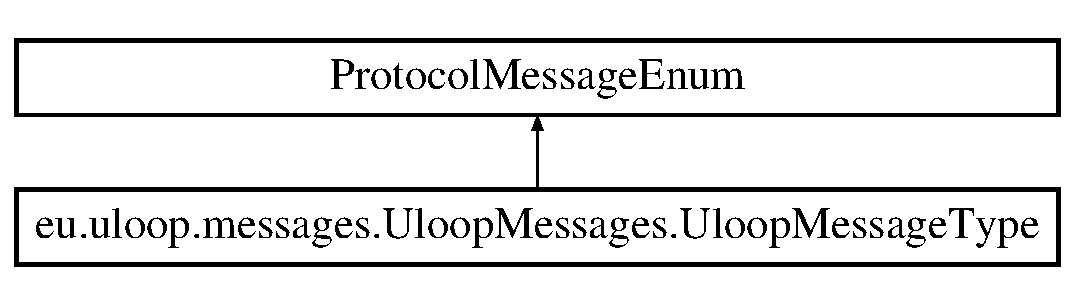
\includegraphics[height=2.000000cm]{enumeu_1_1uloop_1_1messages_1_1UloopMessages_1_1UloopMessageType}
\end{center}
\end{figure}
\subsection*{Public Member Functions}
\begin{DoxyCompactItemize}
\item 
final int \hyperlink{enumeu_1_1uloop_1_1messages_1_1UloopMessages_1_1UloopMessageType_abcc6d8ac19328ab0a00f00f7048a8eae}{get\+Number} ()
\item 
final \\*
com.\+google.\+protobuf.\+Descriptors.\+Enum\+Value\+Descriptor \hyperlink{enumeu_1_1uloop_1_1messages_1_1UloopMessages_1_1UloopMessageType_a267033fca5257cd3b9c671114828e754}{get\+Value\+Descriptor} ()
\item 
final \\*
com.\+google.\+protobuf.\+Descriptors.\+Enum\+Descriptor \hyperlink{enumeu_1_1uloop_1_1messages_1_1UloopMessages_1_1UloopMessageType_a0a5b813f886253f042d45af35eb85772}{get\+Descriptor\+For\+Type} ()
\end{DoxyCompactItemize}
\subsection*{Static Public Member Functions}
\begin{DoxyCompactItemize}
\item 
static \hyperlink{enumeu_1_1uloop_1_1messages_1_1UloopMessages_1_1UloopMessageType}{Uloop\+Message\+Type} \hyperlink{enumeu_1_1uloop_1_1messages_1_1UloopMessages_1_1UloopMessageType_aba3200220ef915b16ae861d0e8a0c246}{value\+Of} (int \hyperlink{enumeu_1_1uloop_1_1messages_1_1UloopMessages_1_1UloopMessageType_a757996108c5d548bcfaf69a86a385761}{value})
\item 
static \\*
com.\+google.\+protobuf.\+Internal.\+Enum\+Lite\+Map\\*
$<$ \hyperlink{enumeu_1_1uloop_1_1messages_1_1UloopMessages_1_1UloopMessageType}{Uloop\+Message\+Type} $>$ \hyperlink{enumeu_1_1uloop_1_1messages_1_1UloopMessages_1_1UloopMessageType_a541a8409b2646f6b3974bb2c9147cef9}{internal\+Get\+Value\+Map} ()
\item 
static final \\*
com.\+google.\+protobuf.\+Descriptors.\+Enum\+Descriptor \hyperlink{enumeu_1_1uloop_1_1messages_1_1UloopMessages_1_1UloopMessageType_ae4788dc7a3795c2952f170dd243e5d0c}{get\+Descriptor} ()
\item 
static \hyperlink{enumeu_1_1uloop_1_1messages_1_1UloopMessages_1_1UloopMessageType}{Uloop\+Message\+Type} \hyperlink{enumeu_1_1uloop_1_1messages_1_1UloopMessages_1_1UloopMessageType_a0158c3665518e84498cc3947b2ba89ab}{value\+Of} (com.\+google.\+protobuf.\+Descriptors.\+Enum\+Value\+Descriptor desc)
\end{DoxyCompactItemize}
\subsection*{Public Attributes}
\begin{DoxyCompactItemize}
\item 
\hyperlink{enumeu_1_1uloop_1_1messages_1_1UloopMessages_1_1UloopMessageType_a457cbfce646e37005987a686aa1f876e}{U\+L\+O\+O\+P\+\_\+\+U\+N\+S\+P\+E\+C} =(0, 0)
\item 
\hyperlink{enumeu_1_1uloop_1_1messages_1_1UloopMessages_1_1UloopMessageType_ad2d2caa5e4a4fd68d44f422b23af44ac}{U\+L\+O\+O\+P\+\_\+\+E\+N\+O\+U\+G\+H\+\_\+\+R\+E\+S\+O\+U\+R\+C\+E\+S} =(1, 1)
\item 
\hyperlink{enumeu_1_1uloop_1_1messages_1_1UloopMessages_1_1UloopMessageType_a7290b987c0c214555491be7c4fc45835}{U\+L\+O\+O\+P\+\_\+\+C\+A\+C\+\_\+\+M\+E\+S\+S\+A\+G\+E} =(2, 2)
\item 
\hyperlink{enumeu_1_1uloop_1_1messages_1_1UloopMessages_1_1UloopMessageType_a4c6be9e1d2048fb126a0c309ed5e8acf}{U\+L\+O\+O\+P\+\_\+\+M\+O\+B\+I\+L\+I\+T\+Y\+\_\+\+R\+M} =(3, 3)
\item 
\hyperlink{enumeu_1_1uloop_1_1messages_1_1UloopMessages_1_1UloopMessageType_acfcddc123ef961d02b619e0e687a625a}{U\+L\+O\+O\+P\+\_\+\+M\+E\+M\+\_\+\+R\+E\+S\+O\+U\+R\+C\+E\+S} =(4, 4)
\item 
\hyperlink{enumeu_1_1uloop_1_1messages_1_1UloopMessages_1_1UloopMessageType_afe52072954431f52c76dfc1abcc26807}{U\+L\+O\+O\+P\+\_\+\+N\+E\+W\+U\+S\+E\+R\+D\+E\+T\+A\+I\+L\+S} =(5, 5)
\item 
\hyperlink{enumeu_1_1uloop_1_1messages_1_1UloopMessages_1_1UloopMessageType_a9e9d5e8074b3576749dcd41a7cc4545c}{U\+L\+O\+O\+P\+\_\+\+N\+E\+T\+W\+O\+R\+K\+S\+T\+A\+T\+U\+S} =(6, 6)
\item 
\hyperlink{enumeu_1_1uloop_1_1messages_1_1UloopMessages_1_1UloopMessageType_a00a2706ce85a9e84cbc0218c55804705}{U\+L\+O\+O\+P\+\_\+\+T\+R\+U\+S\+T\+M\+E\+S\+S\+A\+G\+E} =(7, 7)
\item 
\hyperlink{enumeu_1_1uloop_1_1messages_1_1UloopMessages_1_1UloopMessageType_ac62db035f61911b6d5a8a1de969cb817}{U\+L\+O\+O\+P\+\_\+\+Q\+O\+S\+M\+E\+S\+S\+A\+G\+E} =(8, 8)
\item 
\hyperlink{enumeu_1_1uloop_1_1messages_1_1UloopMessages_1_1UloopMessageType_a2e48a358b6ba1af599146c95c4449b09}{U\+L\+O\+O\+P\+\_\+\+E\+X\+T\+E\+R\+N\+A\+L\+\_\+\+S\+E\+R\+V\+I\+C\+E} =(9, 9)
\item 
\hyperlink{enumeu_1_1uloop_1_1messages_1_1UloopMessages_1_1UloopMessageType_a5279fcb970ff6e20df2536163d3cd33a}{U\+L\+O\+O\+P\+\_\+\+E\+X\+T\+E\+R\+N\+A\+L\+\_\+\+M\+T\+R\+A\+C\+K\+E\+R} =(10, 10)
\end{DoxyCompactItemize}
\subsection*{Static Public Attributes}
\begin{DoxyCompactItemize}
\item 
staticfinal int \hyperlink{enumeu_1_1uloop_1_1messages_1_1UloopMessages_1_1UloopMessageType_a47fabf998a195f19f247304313b3f85e}{U\+L\+O\+O\+P\+\_\+\+U\+N\+S\+P\+E\+C\+\_\+\+V\+A\+L\+U\+E} = 0
\item 
staticfinal int \hyperlink{enumeu_1_1uloop_1_1messages_1_1UloopMessages_1_1UloopMessageType_a189a09fd86d165c2b0852f7c8ee625d0}{U\+L\+O\+O\+P\+\_\+\+E\+N\+O\+U\+G\+H\+\_\+\+R\+E\+S\+O\+U\+R\+C\+E\+S\+\_\+\+V\+A\+L\+U\+E} = 1
\item 
staticfinal int \hyperlink{enumeu_1_1uloop_1_1messages_1_1UloopMessages_1_1UloopMessageType_a49adc846b939f464602acea9e01c6e71}{U\+L\+O\+O\+P\+\_\+\+C\+A\+C\+\_\+\+M\+E\+S\+S\+A\+G\+E\+\_\+\+V\+A\+L\+U\+E} = 2
\item 
staticfinal int \hyperlink{enumeu_1_1uloop_1_1messages_1_1UloopMessages_1_1UloopMessageType_a01d2cd97565263fb97363f784dcf804b}{U\+L\+O\+O\+P\+\_\+\+M\+O\+B\+I\+L\+I\+T\+Y\+\_\+\+R\+M\+\_\+\+V\+A\+L\+U\+E} = 3
\item 
staticfinal int \hyperlink{enumeu_1_1uloop_1_1messages_1_1UloopMessages_1_1UloopMessageType_a55a93bf1e295176e0b5c8855804ab5f3}{U\+L\+O\+O\+P\+\_\+\+M\+E\+M\+\_\+\+R\+E\+S\+O\+U\+R\+C\+E\+S\+\_\+\+V\+A\+L\+U\+E} = 4
\item 
staticfinal int \hyperlink{enumeu_1_1uloop_1_1messages_1_1UloopMessages_1_1UloopMessageType_a41cc14787d3152d2b3e260d569366e9c}{U\+L\+O\+O\+P\+\_\+\+N\+E\+W\+U\+S\+E\+R\+D\+E\+T\+A\+I\+L\+S\+\_\+\+V\+A\+L\+U\+E} = 5
\item 
staticfinal int \hyperlink{enumeu_1_1uloop_1_1messages_1_1UloopMessages_1_1UloopMessageType_a254b62dd08201d1eba1c90bdaa0c08f7}{U\+L\+O\+O\+P\+\_\+\+N\+E\+T\+W\+O\+R\+K\+S\+T\+A\+T\+U\+S\+\_\+\+V\+A\+L\+U\+E} = 6
\item 
staticfinal int \hyperlink{enumeu_1_1uloop_1_1messages_1_1UloopMessages_1_1UloopMessageType_a8b25a66b59c2505ee11bca2164b2e83d}{U\+L\+O\+O\+P\+\_\+\+T\+R\+U\+S\+T\+M\+E\+S\+S\+A\+G\+E\+\_\+\+V\+A\+L\+U\+E} = 7
\item 
staticfinal int \hyperlink{enumeu_1_1uloop_1_1messages_1_1UloopMessages_1_1UloopMessageType_a89d68e3c0962d286dea85b6f1280b82c}{U\+L\+O\+O\+P\+\_\+\+Q\+O\+S\+M\+E\+S\+S\+A\+G\+E\+\_\+\+V\+A\+L\+U\+E} = 8
\item 
staticfinal int \hyperlink{enumeu_1_1uloop_1_1messages_1_1UloopMessages_1_1UloopMessageType_acf5d5ff984b25052735b75ec79271fba}{U\+L\+O\+O\+P\+\_\+\+E\+X\+T\+E\+R\+N\+A\+L\+\_\+\+S\+E\+R\+V\+I\+C\+E\+\_\+\+V\+A\+L\+U\+E} = 9
\item 
staticfinal int \hyperlink{enumeu_1_1uloop_1_1messages_1_1UloopMessages_1_1UloopMessageType_a4f9777bb27c76f61628926bedc37a25d}{U\+L\+O\+O\+P\+\_\+\+E\+X\+T\+E\+R\+N\+A\+L\+\_\+\+M\+T\+R\+A\+C\+K\+E\+R\+\_\+\+V\+A\+L\+U\+E} = 10
\end{DoxyCompactItemize}
\subsection*{Private Member Functions}
\begin{DoxyCompactItemize}
\item 
\hyperlink{enumeu_1_1uloop_1_1messages_1_1UloopMessages_1_1UloopMessageType_a47bcc9408a8b6ebadc16ecf51e38ab5a}{Uloop\+Message\+Type} (int \hyperlink{enumeu_1_1uloop_1_1messages_1_1UloopMessages_1_1UloopMessageType_aec1ce079512854d8a1e703fe37dcfd29}{index}, int \hyperlink{enumeu_1_1uloop_1_1messages_1_1UloopMessages_1_1UloopMessageType_a757996108c5d548bcfaf69a86a385761}{value})
\end{DoxyCompactItemize}
\subsection*{Private Attributes}
\begin{DoxyCompactItemize}
\item 
final int \hyperlink{enumeu_1_1uloop_1_1messages_1_1UloopMessages_1_1UloopMessageType_aec1ce079512854d8a1e703fe37dcfd29}{index}
\item 
final int \hyperlink{enumeu_1_1uloop_1_1messages_1_1UloopMessages_1_1UloopMessageType_a757996108c5d548bcfaf69a86a385761}{value}
\end{DoxyCompactItemize}
\subsection*{Static Private Attributes}
\begin{DoxyCompactItemize}
\item 
staticcom.\+google.\+protobuf.\+Internal.\+Enum\+Lite\+Map\\*
$<$ \hyperlink{enumeu_1_1uloop_1_1messages_1_1UloopMessages_1_1UloopMessageType}{Uloop\+Message\+Type} $>$ \hyperlink{enumeu_1_1uloop_1_1messages_1_1UloopMessages_1_1UloopMessageType_afb6e1f733b8bcb79ab024acc56156437}{internal\+Value\+Map}
\item 
staticfinal \hyperlink{enumeu_1_1uloop_1_1messages_1_1UloopMessages_1_1UloopMessageType}{Uloop\+Message\+Type}\mbox{[}$\,$\mbox{]} \hyperlink{enumeu_1_1uloop_1_1messages_1_1UloopMessages_1_1UloopMessageType_acba7a3d491de5b16d9963b763ed919ee}{V\+A\+L\+U\+E\+S}
\end{DoxyCompactItemize}


\subsection{Constructor \& Destructor Documentation}
\hypertarget{enumeu_1_1uloop_1_1messages_1_1UloopMessages_1_1UloopMessageType_a47bcc9408a8b6ebadc16ecf51e38ab5a}{\index{eu\+::uloop\+::messages\+::\+Uloop\+Messages\+::\+Uloop\+Message\+Type@{eu\+::uloop\+::messages\+::\+Uloop\+Messages\+::\+Uloop\+Message\+Type}!Uloop\+Message\+Type@{Uloop\+Message\+Type}}
\index{Uloop\+Message\+Type@{Uloop\+Message\+Type}!eu\+::uloop\+::messages\+::\+Uloop\+Messages\+::\+Uloop\+Message\+Type@{eu\+::uloop\+::messages\+::\+Uloop\+Messages\+::\+Uloop\+Message\+Type}}
\subsubsection[{Uloop\+Message\+Type}]{\setlength{\rightskip}{0pt plus 5cm}eu.\+uloop.\+messages.\+Uloop\+Messages.\+Uloop\+Message\+Type.\+Uloop\+Message\+Type (
\begin{DoxyParamCaption}
\item[{int}]{index, }
\item[{int}]{value}
\end{DoxyParamCaption}
)\hspace{0.3cm}{\ttfamily [private]}}}\label{enumeu_1_1uloop_1_1messages_1_1UloopMessages_1_1UloopMessageType_a47bcc9408a8b6ebadc16ecf51e38ab5a}


\subsection{Member Function Documentation}
\hypertarget{enumeu_1_1uloop_1_1messages_1_1UloopMessages_1_1UloopMessageType_ae4788dc7a3795c2952f170dd243e5d0c}{\index{eu\+::uloop\+::messages\+::\+Uloop\+Messages\+::\+Uloop\+Message\+Type@{eu\+::uloop\+::messages\+::\+Uloop\+Messages\+::\+Uloop\+Message\+Type}!get\+Descriptor@{get\+Descriptor}}
\index{get\+Descriptor@{get\+Descriptor}!eu\+::uloop\+::messages\+::\+Uloop\+Messages\+::\+Uloop\+Message\+Type@{eu\+::uloop\+::messages\+::\+Uloop\+Messages\+::\+Uloop\+Message\+Type}}
\subsubsection[{get\+Descriptor}]{\setlength{\rightskip}{0pt plus 5cm}static final com.\+google.\+protobuf.\+Descriptors.\+Enum\+Descriptor eu.\+uloop.\+messages.\+Uloop\+Messages.\+Uloop\+Message\+Type.\+get\+Descriptor (
\begin{DoxyParamCaption}
{}
\end{DoxyParamCaption}
)\hspace{0.3cm}{\ttfamily [static]}}}\label{enumeu_1_1uloop_1_1messages_1_1UloopMessages_1_1UloopMessageType_ae4788dc7a3795c2952f170dd243e5d0c}
\hypertarget{enumeu_1_1uloop_1_1messages_1_1UloopMessages_1_1UloopMessageType_a0a5b813f886253f042d45af35eb85772}{\index{eu\+::uloop\+::messages\+::\+Uloop\+Messages\+::\+Uloop\+Message\+Type@{eu\+::uloop\+::messages\+::\+Uloop\+Messages\+::\+Uloop\+Message\+Type}!get\+Descriptor\+For\+Type@{get\+Descriptor\+For\+Type}}
\index{get\+Descriptor\+For\+Type@{get\+Descriptor\+For\+Type}!eu\+::uloop\+::messages\+::\+Uloop\+Messages\+::\+Uloop\+Message\+Type@{eu\+::uloop\+::messages\+::\+Uloop\+Messages\+::\+Uloop\+Message\+Type}}
\subsubsection[{get\+Descriptor\+For\+Type}]{\setlength{\rightskip}{0pt plus 5cm}final com.\+google.\+protobuf.\+Descriptors.\+Enum\+Descriptor eu.\+uloop.\+messages.\+Uloop\+Messages.\+Uloop\+Message\+Type.\+get\+Descriptor\+For\+Type (
\begin{DoxyParamCaption}
{}
\end{DoxyParamCaption}
)}}\label{enumeu_1_1uloop_1_1messages_1_1UloopMessages_1_1UloopMessageType_a0a5b813f886253f042d45af35eb85772}
\hypertarget{enumeu_1_1uloop_1_1messages_1_1UloopMessages_1_1UloopMessageType_abcc6d8ac19328ab0a00f00f7048a8eae}{\index{eu\+::uloop\+::messages\+::\+Uloop\+Messages\+::\+Uloop\+Message\+Type@{eu\+::uloop\+::messages\+::\+Uloop\+Messages\+::\+Uloop\+Message\+Type}!get\+Number@{get\+Number}}
\index{get\+Number@{get\+Number}!eu\+::uloop\+::messages\+::\+Uloop\+Messages\+::\+Uloop\+Message\+Type@{eu\+::uloop\+::messages\+::\+Uloop\+Messages\+::\+Uloop\+Message\+Type}}
\subsubsection[{get\+Number}]{\setlength{\rightskip}{0pt plus 5cm}final int eu.\+uloop.\+messages.\+Uloop\+Messages.\+Uloop\+Message\+Type.\+get\+Number (
\begin{DoxyParamCaption}
{}
\end{DoxyParamCaption}
)}}\label{enumeu_1_1uloop_1_1messages_1_1UloopMessages_1_1UloopMessageType_abcc6d8ac19328ab0a00f00f7048a8eae}
\hypertarget{enumeu_1_1uloop_1_1messages_1_1UloopMessages_1_1UloopMessageType_a267033fca5257cd3b9c671114828e754}{\index{eu\+::uloop\+::messages\+::\+Uloop\+Messages\+::\+Uloop\+Message\+Type@{eu\+::uloop\+::messages\+::\+Uloop\+Messages\+::\+Uloop\+Message\+Type}!get\+Value\+Descriptor@{get\+Value\+Descriptor}}
\index{get\+Value\+Descriptor@{get\+Value\+Descriptor}!eu\+::uloop\+::messages\+::\+Uloop\+Messages\+::\+Uloop\+Message\+Type@{eu\+::uloop\+::messages\+::\+Uloop\+Messages\+::\+Uloop\+Message\+Type}}
\subsubsection[{get\+Value\+Descriptor}]{\setlength{\rightskip}{0pt plus 5cm}final com.\+google.\+protobuf.\+Descriptors.\+Enum\+Value\+Descriptor eu.\+uloop.\+messages.\+Uloop\+Messages.\+Uloop\+Message\+Type.\+get\+Value\+Descriptor (
\begin{DoxyParamCaption}
{}
\end{DoxyParamCaption}
)}}\label{enumeu_1_1uloop_1_1messages_1_1UloopMessages_1_1UloopMessageType_a267033fca5257cd3b9c671114828e754}
\hypertarget{enumeu_1_1uloop_1_1messages_1_1UloopMessages_1_1UloopMessageType_a541a8409b2646f6b3974bb2c9147cef9}{\index{eu\+::uloop\+::messages\+::\+Uloop\+Messages\+::\+Uloop\+Message\+Type@{eu\+::uloop\+::messages\+::\+Uloop\+Messages\+::\+Uloop\+Message\+Type}!internal\+Get\+Value\+Map@{internal\+Get\+Value\+Map}}
\index{internal\+Get\+Value\+Map@{internal\+Get\+Value\+Map}!eu\+::uloop\+::messages\+::\+Uloop\+Messages\+::\+Uloop\+Message\+Type@{eu\+::uloop\+::messages\+::\+Uloop\+Messages\+::\+Uloop\+Message\+Type}}
\subsubsection[{internal\+Get\+Value\+Map}]{\setlength{\rightskip}{0pt plus 5cm}static com.\+google.\+protobuf.\+Internal.\+Enum\+Lite\+Map$<${\bf Uloop\+Message\+Type}$>$ eu.\+uloop.\+messages.\+Uloop\+Messages.\+Uloop\+Message\+Type.\+internal\+Get\+Value\+Map (
\begin{DoxyParamCaption}
{}
\end{DoxyParamCaption}
)\hspace{0.3cm}{\ttfamily [static]}}}\label{enumeu_1_1uloop_1_1messages_1_1UloopMessages_1_1UloopMessageType_a541a8409b2646f6b3974bb2c9147cef9}
\hypertarget{enumeu_1_1uloop_1_1messages_1_1UloopMessages_1_1UloopMessageType_aba3200220ef915b16ae861d0e8a0c246}{\index{eu\+::uloop\+::messages\+::\+Uloop\+Messages\+::\+Uloop\+Message\+Type@{eu\+::uloop\+::messages\+::\+Uloop\+Messages\+::\+Uloop\+Message\+Type}!value\+Of@{value\+Of}}
\index{value\+Of@{value\+Of}!eu\+::uloop\+::messages\+::\+Uloop\+Messages\+::\+Uloop\+Message\+Type@{eu\+::uloop\+::messages\+::\+Uloop\+Messages\+::\+Uloop\+Message\+Type}}
\subsubsection[{value\+Of}]{\setlength{\rightskip}{0pt plus 5cm}static {\bf Uloop\+Message\+Type} eu.\+uloop.\+messages.\+Uloop\+Messages.\+Uloop\+Message\+Type.\+value\+Of (
\begin{DoxyParamCaption}
\item[{int}]{value}
\end{DoxyParamCaption}
)\hspace{0.3cm}{\ttfamily [static]}}}\label{enumeu_1_1uloop_1_1messages_1_1UloopMessages_1_1UloopMessageType_aba3200220ef915b16ae861d0e8a0c246}
\hypertarget{enumeu_1_1uloop_1_1messages_1_1UloopMessages_1_1UloopMessageType_a0158c3665518e84498cc3947b2ba89ab}{\index{eu\+::uloop\+::messages\+::\+Uloop\+Messages\+::\+Uloop\+Message\+Type@{eu\+::uloop\+::messages\+::\+Uloop\+Messages\+::\+Uloop\+Message\+Type}!value\+Of@{value\+Of}}
\index{value\+Of@{value\+Of}!eu\+::uloop\+::messages\+::\+Uloop\+Messages\+::\+Uloop\+Message\+Type@{eu\+::uloop\+::messages\+::\+Uloop\+Messages\+::\+Uloop\+Message\+Type}}
\subsubsection[{value\+Of}]{\setlength{\rightskip}{0pt plus 5cm}static {\bf Uloop\+Message\+Type} eu.\+uloop.\+messages.\+Uloop\+Messages.\+Uloop\+Message\+Type.\+value\+Of (
\begin{DoxyParamCaption}
\item[{com.\+google.\+protobuf.\+Descriptors.\+Enum\+Value\+Descriptor}]{desc}
\end{DoxyParamCaption}
)\hspace{0.3cm}{\ttfamily [static]}}}\label{enumeu_1_1uloop_1_1messages_1_1UloopMessages_1_1UloopMessageType_a0158c3665518e84498cc3947b2ba89ab}


\subsection{Member Data Documentation}
\hypertarget{enumeu_1_1uloop_1_1messages_1_1UloopMessages_1_1UloopMessageType_aec1ce079512854d8a1e703fe37dcfd29}{\index{eu\+::uloop\+::messages\+::\+Uloop\+Messages\+::\+Uloop\+Message\+Type@{eu\+::uloop\+::messages\+::\+Uloop\+Messages\+::\+Uloop\+Message\+Type}!index@{index}}
\index{index@{index}!eu\+::uloop\+::messages\+::\+Uloop\+Messages\+::\+Uloop\+Message\+Type@{eu\+::uloop\+::messages\+::\+Uloop\+Messages\+::\+Uloop\+Message\+Type}}
\subsubsection[{index}]{\setlength{\rightskip}{0pt plus 5cm}final int eu.\+uloop.\+messages.\+Uloop\+Messages.\+Uloop\+Message\+Type.\+index\hspace{0.3cm}{\ttfamily [private]}}}\label{enumeu_1_1uloop_1_1messages_1_1UloopMessages_1_1UloopMessageType_aec1ce079512854d8a1e703fe37dcfd29}
\hypertarget{enumeu_1_1uloop_1_1messages_1_1UloopMessages_1_1UloopMessageType_afb6e1f733b8bcb79ab024acc56156437}{\index{eu\+::uloop\+::messages\+::\+Uloop\+Messages\+::\+Uloop\+Message\+Type@{eu\+::uloop\+::messages\+::\+Uloop\+Messages\+::\+Uloop\+Message\+Type}!internal\+Value\+Map@{internal\+Value\+Map}}
\index{internal\+Value\+Map@{internal\+Value\+Map}!eu\+::uloop\+::messages\+::\+Uloop\+Messages\+::\+Uloop\+Message\+Type@{eu\+::uloop\+::messages\+::\+Uloop\+Messages\+::\+Uloop\+Message\+Type}}
\subsubsection[{internal\+Value\+Map}]{\setlength{\rightskip}{0pt plus 5cm} static  com.\+google.\+protobuf.\+Internal.\+Enum\+Lite\+Map$<${\bf Uloop\+Message\+Type}$>$ eu.\+uloop.\+messages.\+Uloop\+Messages.\+Uloop\+Message\+Type.\+internal\+Value\+Map\hspace{0.3cm}{\ttfamily [static]}, {\ttfamily [private]}}}\label{enumeu_1_1uloop_1_1messages_1_1UloopMessages_1_1UloopMessageType_afb6e1f733b8bcb79ab024acc56156437}
{\bfseries Initial value\+:}
\begin{DoxyCode}
=
          \textcolor{keyword}{new} com.google.protobuf.Internal.EnumLiteMap<\hyperlink{enumeu_1_1uloop_1_1messages_1_1UloopMessages_1_1UloopMessageType_a47bcc9408a8b6ebadc16ecf51e38ab5a}{UloopMessageType}>() \{
            \textcolor{keyword}{public} \hyperlink{enumeu_1_1uloop_1_1messages_1_1UloopMessages_1_1UloopMessageType_a47bcc9408a8b6ebadc16ecf51e38ab5a}{UloopMessageType} findValueByNumber(\textcolor{keywordtype}{int} number) \{
              \textcolor{keywordflow}{return} \hyperlink{enumeu_1_1uloop_1_1messages_1_1UloopMessages_1_1UloopMessageType_a47bcc9408a8b6ebadc16ecf51e38ab5a}{UloopMessageType}.valueOf(number);
            \}
          \}
\end{DoxyCode}
\hypertarget{enumeu_1_1uloop_1_1messages_1_1UloopMessages_1_1UloopMessageType_a7290b987c0c214555491be7c4fc45835}{\index{eu\+::uloop\+::messages\+::\+Uloop\+Messages\+::\+Uloop\+Message\+Type@{eu\+::uloop\+::messages\+::\+Uloop\+Messages\+::\+Uloop\+Message\+Type}!U\+L\+O\+O\+P\+\_\+\+C\+A\+C\+\_\+\+M\+E\+S\+S\+A\+G\+E@{U\+L\+O\+O\+P\+\_\+\+C\+A\+C\+\_\+\+M\+E\+S\+S\+A\+G\+E}}
\index{U\+L\+O\+O\+P\+\_\+\+C\+A\+C\+\_\+\+M\+E\+S\+S\+A\+G\+E@{U\+L\+O\+O\+P\+\_\+\+C\+A\+C\+\_\+\+M\+E\+S\+S\+A\+G\+E}!eu\+::uloop\+::messages\+::\+Uloop\+Messages\+::\+Uloop\+Message\+Type@{eu\+::uloop\+::messages\+::\+Uloop\+Messages\+::\+Uloop\+Message\+Type}}
\subsubsection[{U\+L\+O\+O\+P\+\_\+\+C\+A\+C\+\_\+\+M\+E\+S\+S\+A\+G\+E}]{\setlength{\rightskip}{0pt plus 5cm}eu.\+uloop.\+messages.\+Uloop\+Messages.\+Uloop\+Message\+Type.\+U\+L\+O\+O\+P\+\_\+\+C\+A\+C\+\_\+\+M\+E\+S\+S\+A\+G\+E =(2, 2)}}\label{enumeu_1_1uloop_1_1messages_1_1UloopMessages_1_1UloopMessageType_a7290b987c0c214555491be7c4fc45835}
\hypertarget{enumeu_1_1uloop_1_1messages_1_1UloopMessages_1_1UloopMessageType_a49adc846b939f464602acea9e01c6e71}{\index{eu\+::uloop\+::messages\+::\+Uloop\+Messages\+::\+Uloop\+Message\+Type@{eu\+::uloop\+::messages\+::\+Uloop\+Messages\+::\+Uloop\+Message\+Type}!U\+L\+O\+O\+P\+\_\+\+C\+A\+C\+\_\+\+M\+E\+S\+S\+A\+G\+E\+\_\+\+V\+A\+L\+U\+E@{U\+L\+O\+O\+P\+\_\+\+C\+A\+C\+\_\+\+M\+E\+S\+S\+A\+G\+E\+\_\+\+V\+A\+L\+U\+E}}
\index{U\+L\+O\+O\+P\+\_\+\+C\+A\+C\+\_\+\+M\+E\+S\+S\+A\+G\+E\+\_\+\+V\+A\+L\+U\+E@{U\+L\+O\+O\+P\+\_\+\+C\+A\+C\+\_\+\+M\+E\+S\+S\+A\+G\+E\+\_\+\+V\+A\+L\+U\+E}!eu\+::uloop\+::messages\+::\+Uloop\+Messages\+::\+Uloop\+Message\+Type@{eu\+::uloop\+::messages\+::\+Uloop\+Messages\+::\+Uloop\+Message\+Type}}
\subsubsection[{U\+L\+O\+O\+P\+\_\+\+C\+A\+C\+\_\+\+M\+E\+S\+S\+A\+G\+E\+\_\+\+V\+A\+L\+U\+E}]{\setlength{\rightskip}{0pt plus 5cm} static  final int eu.\+uloop.\+messages.\+Uloop\+Messages.\+Uloop\+Message\+Type.\+U\+L\+O\+O\+P\+\_\+\+C\+A\+C\+\_\+\+M\+E\+S\+S\+A\+G\+E\+\_\+\+V\+A\+L\+U\+E = 2\hspace{0.3cm}{\ttfamily [static]}}}\label{enumeu_1_1uloop_1_1messages_1_1UloopMessages_1_1UloopMessageType_a49adc846b939f464602acea9e01c6e71}
\hypertarget{enumeu_1_1uloop_1_1messages_1_1UloopMessages_1_1UloopMessageType_ad2d2caa5e4a4fd68d44f422b23af44ac}{\index{eu\+::uloop\+::messages\+::\+Uloop\+Messages\+::\+Uloop\+Message\+Type@{eu\+::uloop\+::messages\+::\+Uloop\+Messages\+::\+Uloop\+Message\+Type}!U\+L\+O\+O\+P\+\_\+\+E\+N\+O\+U\+G\+H\+\_\+\+R\+E\+S\+O\+U\+R\+C\+E\+S@{U\+L\+O\+O\+P\+\_\+\+E\+N\+O\+U\+G\+H\+\_\+\+R\+E\+S\+O\+U\+R\+C\+E\+S}}
\index{U\+L\+O\+O\+P\+\_\+\+E\+N\+O\+U\+G\+H\+\_\+\+R\+E\+S\+O\+U\+R\+C\+E\+S@{U\+L\+O\+O\+P\+\_\+\+E\+N\+O\+U\+G\+H\+\_\+\+R\+E\+S\+O\+U\+R\+C\+E\+S}!eu\+::uloop\+::messages\+::\+Uloop\+Messages\+::\+Uloop\+Message\+Type@{eu\+::uloop\+::messages\+::\+Uloop\+Messages\+::\+Uloop\+Message\+Type}}
\subsubsection[{U\+L\+O\+O\+P\+\_\+\+E\+N\+O\+U\+G\+H\+\_\+\+R\+E\+S\+O\+U\+R\+C\+E\+S}]{\setlength{\rightskip}{0pt plus 5cm}eu.\+uloop.\+messages.\+Uloop\+Messages.\+Uloop\+Message\+Type.\+U\+L\+O\+O\+P\+\_\+\+E\+N\+O\+U\+G\+H\+\_\+\+R\+E\+S\+O\+U\+R\+C\+E\+S =(1, 1)}}\label{enumeu_1_1uloop_1_1messages_1_1UloopMessages_1_1UloopMessageType_ad2d2caa5e4a4fd68d44f422b23af44ac}
\hypertarget{enumeu_1_1uloop_1_1messages_1_1UloopMessages_1_1UloopMessageType_a189a09fd86d165c2b0852f7c8ee625d0}{\index{eu\+::uloop\+::messages\+::\+Uloop\+Messages\+::\+Uloop\+Message\+Type@{eu\+::uloop\+::messages\+::\+Uloop\+Messages\+::\+Uloop\+Message\+Type}!U\+L\+O\+O\+P\+\_\+\+E\+N\+O\+U\+G\+H\+\_\+\+R\+E\+S\+O\+U\+R\+C\+E\+S\+\_\+\+V\+A\+L\+U\+E@{U\+L\+O\+O\+P\+\_\+\+E\+N\+O\+U\+G\+H\+\_\+\+R\+E\+S\+O\+U\+R\+C\+E\+S\+\_\+\+V\+A\+L\+U\+E}}
\index{U\+L\+O\+O\+P\+\_\+\+E\+N\+O\+U\+G\+H\+\_\+\+R\+E\+S\+O\+U\+R\+C\+E\+S\+\_\+\+V\+A\+L\+U\+E@{U\+L\+O\+O\+P\+\_\+\+E\+N\+O\+U\+G\+H\+\_\+\+R\+E\+S\+O\+U\+R\+C\+E\+S\+\_\+\+V\+A\+L\+U\+E}!eu\+::uloop\+::messages\+::\+Uloop\+Messages\+::\+Uloop\+Message\+Type@{eu\+::uloop\+::messages\+::\+Uloop\+Messages\+::\+Uloop\+Message\+Type}}
\subsubsection[{U\+L\+O\+O\+P\+\_\+\+E\+N\+O\+U\+G\+H\+\_\+\+R\+E\+S\+O\+U\+R\+C\+E\+S\+\_\+\+V\+A\+L\+U\+E}]{\setlength{\rightskip}{0pt plus 5cm} static  final int eu.\+uloop.\+messages.\+Uloop\+Messages.\+Uloop\+Message\+Type.\+U\+L\+O\+O\+P\+\_\+\+E\+N\+O\+U\+G\+H\+\_\+\+R\+E\+S\+O\+U\+R\+C\+E\+S\+\_\+\+V\+A\+L\+U\+E = 1\hspace{0.3cm}{\ttfamily [static]}}}\label{enumeu_1_1uloop_1_1messages_1_1UloopMessages_1_1UloopMessageType_a189a09fd86d165c2b0852f7c8ee625d0}
\hypertarget{enumeu_1_1uloop_1_1messages_1_1UloopMessages_1_1UloopMessageType_a5279fcb970ff6e20df2536163d3cd33a}{\index{eu\+::uloop\+::messages\+::\+Uloop\+Messages\+::\+Uloop\+Message\+Type@{eu\+::uloop\+::messages\+::\+Uloop\+Messages\+::\+Uloop\+Message\+Type}!U\+L\+O\+O\+P\+\_\+\+E\+X\+T\+E\+R\+N\+A\+L\+\_\+\+M\+T\+R\+A\+C\+K\+E\+R@{U\+L\+O\+O\+P\+\_\+\+E\+X\+T\+E\+R\+N\+A\+L\+\_\+\+M\+T\+R\+A\+C\+K\+E\+R}}
\index{U\+L\+O\+O\+P\+\_\+\+E\+X\+T\+E\+R\+N\+A\+L\+\_\+\+M\+T\+R\+A\+C\+K\+E\+R@{U\+L\+O\+O\+P\+\_\+\+E\+X\+T\+E\+R\+N\+A\+L\+\_\+\+M\+T\+R\+A\+C\+K\+E\+R}!eu\+::uloop\+::messages\+::\+Uloop\+Messages\+::\+Uloop\+Message\+Type@{eu\+::uloop\+::messages\+::\+Uloop\+Messages\+::\+Uloop\+Message\+Type}}
\subsubsection[{U\+L\+O\+O\+P\+\_\+\+E\+X\+T\+E\+R\+N\+A\+L\+\_\+\+M\+T\+R\+A\+C\+K\+E\+R}]{\setlength{\rightskip}{0pt plus 5cm}eu.\+uloop.\+messages.\+Uloop\+Messages.\+Uloop\+Message\+Type.\+U\+L\+O\+O\+P\+\_\+\+E\+X\+T\+E\+R\+N\+A\+L\+\_\+\+M\+T\+R\+A\+C\+K\+E\+R =(10, 10)}}\label{enumeu_1_1uloop_1_1messages_1_1UloopMessages_1_1UloopMessageType_a5279fcb970ff6e20df2536163d3cd33a}
\hypertarget{enumeu_1_1uloop_1_1messages_1_1UloopMessages_1_1UloopMessageType_a4f9777bb27c76f61628926bedc37a25d}{\index{eu\+::uloop\+::messages\+::\+Uloop\+Messages\+::\+Uloop\+Message\+Type@{eu\+::uloop\+::messages\+::\+Uloop\+Messages\+::\+Uloop\+Message\+Type}!U\+L\+O\+O\+P\+\_\+\+E\+X\+T\+E\+R\+N\+A\+L\+\_\+\+M\+T\+R\+A\+C\+K\+E\+R\+\_\+\+V\+A\+L\+U\+E@{U\+L\+O\+O\+P\+\_\+\+E\+X\+T\+E\+R\+N\+A\+L\+\_\+\+M\+T\+R\+A\+C\+K\+E\+R\+\_\+\+V\+A\+L\+U\+E}}
\index{U\+L\+O\+O\+P\+\_\+\+E\+X\+T\+E\+R\+N\+A\+L\+\_\+\+M\+T\+R\+A\+C\+K\+E\+R\+\_\+\+V\+A\+L\+U\+E@{U\+L\+O\+O\+P\+\_\+\+E\+X\+T\+E\+R\+N\+A\+L\+\_\+\+M\+T\+R\+A\+C\+K\+E\+R\+\_\+\+V\+A\+L\+U\+E}!eu\+::uloop\+::messages\+::\+Uloop\+Messages\+::\+Uloop\+Message\+Type@{eu\+::uloop\+::messages\+::\+Uloop\+Messages\+::\+Uloop\+Message\+Type}}
\subsubsection[{U\+L\+O\+O\+P\+\_\+\+E\+X\+T\+E\+R\+N\+A\+L\+\_\+\+M\+T\+R\+A\+C\+K\+E\+R\+\_\+\+V\+A\+L\+U\+E}]{\setlength{\rightskip}{0pt plus 5cm} static  final int eu.\+uloop.\+messages.\+Uloop\+Messages.\+Uloop\+Message\+Type.\+U\+L\+O\+O\+P\+\_\+\+E\+X\+T\+E\+R\+N\+A\+L\+\_\+\+M\+T\+R\+A\+C\+K\+E\+R\+\_\+\+V\+A\+L\+U\+E = 10\hspace{0.3cm}{\ttfamily [static]}}}\label{enumeu_1_1uloop_1_1messages_1_1UloopMessages_1_1UloopMessageType_a4f9777bb27c76f61628926bedc37a25d}
\hypertarget{enumeu_1_1uloop_1_1messages_1_1UloopMessages_1_1UloopMessageType_a2e48a358b6ba1af599146c95c4449b09}{\index{eu\+::uloop\+::messages\+::\+Uloop\+Messages\+::\+Uloop\+Message\+Type@{eu\+::uloop\+::messages\+::\+Uloop\+Messages\+::\+Uloop\+Message\+Type}!U\+L\+O\+O\+P\+\_\+\+E\+X\+T\+E\+R\+N\+A\+L\+\_\+\+S\+E\+R\+V\+I\+C\+E@{U\+L\+O\+O\+P\+\_\+\+E\+X\+T\+E\+R\+N\+A\+L\+\_\+\+S\+E\+R\+V\+I\+C\+E}}
\index{U\+L\+O\+O\+P\+\_\+\+E\+X\+T\+E\+R\+N\+A\+L\+\_\+\+S\+E\+R\+V\+I\+C\+E@{U\+L\+O\+O\+P\+\_\+\+E\+X\+T\+E\+R\+N\+A\+L\+\_\+\+S\+E\+R\+V\+I\+C\+E}!eu\+::uloop\+::messages\+::\+Uloop\+Messages\+::\+Uloop\+Message\+Type@{eu\+::uloop\+::messages\+::\+Uloop\+Messages\+::\+Uloop\+Message\+Type}}
\subsubsection[{U\+L\+O\+O\+P\+\_\+\+E\+X\+T\+E\+R\+N\+A\+L\+\_\+\+S\+E\+R\+V\+I\+C\+E}]{\setlength{\rightskip}{0pt plus 5cm}eu.\+uloop.\+messages.\+Uloop\+Messages.\+Uloop\+Message\+Type.\+U\+L\+O\+O\+P\+\_\+\+E\+X\+T\+E\+R\+N\+A\+L\+\_\+\+S\+E\+R\+V\+I\+C\+E =(9, 9)}}\label{enumeu_1_1uloop_1_1messages_1_1UloopMessages_1_1UloopMessageType_a2e48a358b6ba1af599146c95c4449b09}
\hypertarget{enumeu_1_1uloop_1_1messages_1_1UloopMessages_1_1UloopMessageType_acf5d5ff984b25052735b75ec79271fba}{\index{eu\+::uloop\+::messages\+::\+Uloop\+Messages\+::\+Uloop\+Message\+Type@{eu\+::uloop\+::messages\+::\+Uloop\+Messages\+::\+Uloop\+Message\+Type}!U\+L\+O\+O\+P\+\_\+\+E\+X\+T\+E\+R\+N\+A\+L\+\_\+\+S\+E\+R\+V\+I\+C\+E\+\_\+\+V\+A\+L\+U\+E@{U\+L\+O\+O\+P\+\_\+\+E\+X\+T\+E\+R\+N\+A\+L\+\_\+\+S\+E\+R\+V\+I\+C\+E\+\_\+\+V\+A\+L\+U\+E}}
\index{U\+L\+O\+O\+P\+\_\+\+E\+X\+T\+E\+R\+N\+A\+L\+\_\+\+S\+E\+R\+V\+I\+C\+E\+\_\+\+V\+A\+L\+U\+E@{U\+L\+O\+O\+P\+\_\+\+E\+X\+T\+E\+R\+N\+A\+L\+\_\+\+S\+E\+R\+V\+I\+C\+E\+\_\+\+V\+A\+L\+U\+E}!eu\+::uloop\+::messages\+::\+Uloop\+Messages\+::\+Uloop\+Message\+Type@{eu\+::uloop\+::messages\+::\+Uloop\+Messages\+::\+Uloop\+Message\+Type}}
\subsubsection[{U\+L\+O\+O\+P\+\_\+\+E\+X\+T\+E\+R\+N\+A\+L\+\_\+\+S\+E\+R\+V\+I\+C\+E\+\_\+\+V\+A\+L\+U\+E}]{\setlength{\rightskip}{0pt plus 5cm} static  final int eu.\+uloop.\+messages.\+Uloop\+Messages.\+Uloop\+Message\+Type.\+U\+L\+O\+O\+P\+\_\+\+E\+X\+T\+E\+R\+N\+A\+L\+\_\+\+S\+E\+R\+V\+I\+C\+E\+\_\+\+V\+A\+L\+U\+E = 9\hspace{0.3cm}{\ttfamily [static]}}}\label{enumeu_1_1uloop_1_1messages_1_1UloopMessages_1_1UloopMessageType_acf5d5ff984b25052735b75ec79271fba}
\hypertarget{enumeu_1_1uloop_1_1messages_1_1UloopMessages_1_1UloopMessageType_acfcddc123ef961d02b619e0e687a625a}{\index{eu\+::uloop\+::messages\+::\+Uloop\+Messages\+::\+Uloop\+Message\+Type@{eu\+::uloop\+::messages\+::\+Uloop\+Messages\+::\+Uloop\+Message\+Type}!U\+L\+O\+O\+P\+\_\+\+M\+E\+M\+\_\+\+R\+E\+S\+O\+U\+R\+C\+E\+S@{U\+L\+O\+O\+P\+\_\+\+M\+E\+M\+\_\+\+R\+E\+S\+O\+U\+R\+C\+E\+S}}
\index{U\+L\+O\+O\+P\+\_\+\+M\+E\+M\+\_\+\+R\+E\+S\+O\+U\+R\+C\+E\+S@{U\+L\+O\+O\+P\+\_\+\+M\+E\+M\+\_\+\+R\+E\+S\+O\+U\+R\+C\+E\+S}!eu\+::uloop\+::messages\+::\+Uloop\+Messages\+::\+Uloop\+Message\+Type@{eu\+::uloop\+::messages\+::\+Uloop\+Messages\+::\+Uloop\+Message\+Type}}
\subsubsection[{U\+L\+O\+O\+P\+\_\+\+M\+E\+M\+\_\+\+R\+E\+S\+O\+U\+R\+C\+E\+S}]{\setlength{\rightskip}{0pt plus 5cm}eu.\+uloop.\+messages.\+Uloop\+Messages.\+Uloop\+Message\+Type.\+U\+L\+O\+O\+P\+\_\+\+M\+E\+M\+\_\+\+R\+E\+S\+O\+U\+R\+C\+E\+S =(4, 4)}}\label{enumeu_1_1uloop_1_1messages_1_1UloopMessages_1_1UloopMessageType_acfcddc123ef961d02b619e0e687a625a}
\hypertarget{enumeu_1_1uloop_1_1messages_1_1UloopMessages_1_1UloopMessageType_a55a93bf1e295176e0b5c8855804ab5f3}{\index{eu\+::uloop\+::messages\+::\+Uloop\+Messages\+::\+Uloop\+Message\+Type@{eu\+::uloop\+::messages\+::\+Uloop\+Messages\+::\+Uloop\+Message\+Type}!U\+L\+O\+O\+P\+\_\+\+M\+E\+M\+\_\+\+R\+E\+S\+O\+U\+R\+C\+E\+S\+\_\+\+V\+A\+L\+U\+E@{U\+L\+O\+O\+P\+\_\+\+M\+E\+M\+\_\+\+R\+E\+S\+O\+U\+R\+C\+E\+S\+\_\+\+V\+A\+L\+U\+E}}
\index{U\+L\+O\+O\+P\+\_\+\+M\+E\+M\+\_\+\+R\+E\+S\+O\+U\+R\+C\+E\+S\+\_\+\+V\+A\+L\+U\+E@{U\+L\+O\+O\+P\+\_\+\+M\+E\+M\+\_\+\+R\+E\+S\+O\+U\+R\+C\+E\+S\+\_\+\+V\+A\+L\+U\+E}!eu\+::uloop\+::messages\+::\+Uloop\+Messages\+::\+Uloop\+Message\+Type@{eu\+::uloop\+::messages\+::\+Uloop\+Messages\+::\+Uloop\+Message\+Type}}
\subsubsection[{U\+L\+O\+O\+P\+\_\+\+M\+E\+M\+\_\+\+R\+E\+S\+O\+U\+R\+C\+E\+S\+\_\+\+V\+A\+L\+U\+E}]{\setlength{\rightskip}{0pt plus 5cm} static  final int eu.\+uloop.\+messages.\+Uloop\+Messages.\+Uloop\+Message\+Type.\+U\+L\+O\+O\+P\+\_\+\+M\+E\+M\+\_\+\+R\+E\+S\+O\+U\+R\+C\+E\+S\+\_\+\+V\+A\+L\+U\+E = 4\hspace{0.3cm}{\ttfamily [static]}}}\label{enumeu_1_1uloop_1_1messages_1_1UloopMessages_1_1UloopMessageType_a55a93bf1e295176e0b5c8855804ab5f3}
\hypertarget{enumeu_1_1uloop_1_1messages_1_1UloopMessages_1_1UloopMessageType_a4c6be9e1d2048fb126a0c309ed5e8acf}{\index{eu\+::uloop\+::messages\+::\+Uloop\+Messages\+::\+Uloop\+Message\+Type@{eu\+::uloop\+::messages\+::\+Uloop\+Messages\+::\+Uloop\+Message\+Type}!U\+L\+O\+O\+P\+\_\+\+M\+O\+B\+I\+L\+I\+T\+Y\+\_\+\+R\+M@{U\+L\+O\+O\+P\+\_\+\+M\+O\+B\+I\+L\+I\+T\+Y\+\_\+\+R\+M}}
\index{U\+L\+O\+O\+P\+\_\+\+M\+O\+B\+I\+L\+I\+T\+Y\+\_\+\+R\+M@{U\+L\+O\+O\+P\+\_\+\+M\+O\+B\+I\+L\+I\+T\+Y\+\_\+\+R\+M}!eu\+::uloop\+::messages\+::\+Uloop\+Messages\+::\+Uloop\+Message\+Type@{eu\+::uloop\+::messages\+::\+Uloop\+Messages\+::\+Uloop\+Message\+Type}}
\subsubsection[{U\+L\+O\+O\+P\+\_\+\+M\+O\+B\+I\+L\+I\+T\+Y\+\_\+\+R\+M}]{\setlength{\rightskip}{0pt plus 5cm}eu.\+uloop.\+messages.\+Uloop\+Messages.\+Uloop\+Message\+Type.\+U\+L\+O\+O\+P\+\_\+\+M\+O\+B\+I\+L\+I\+T\+Y\+\_\+\+R\+M =(3, 3)}}\label{enumeu_1_1uloop_1_1messages_1_1UloopMessages_1_1UloopMessageType_a4c6be9e1d2048fb126a0c309ed5e8acf}
\hypertarget{enumeu_1_1uloop_1_1messages_1_1UloopMessages_1_1UloopMessageType_a01d2cd97565263fb97363f784dcf804b}{\index{eu\+::uloop\+::messages\+::\+Uloop\+Messages\+::\+Uloop\+Message\+Type@{eu\+::uloop\+::messages\+::\+Uloop\+Messages\+::\+Uloop\+Message\+Type}!U\+L\+O\+O\+P\+\_\+\+M\+O\+B\+I\+L\+I\+T\+Y\+\_\+\+R\+M\+\_\+\+V\+A\+L\+U\+E@{U\+L\+O\+O\+P\+\_\+\+M\+O\+B\+I\+L\+I\+T\+Y\+\_\+\+R\+M\+\_\+\+V\+A\+L\+U\+E}}
\index{U\+L\+O\+O\+P\+\_\+\+M\+O\+B\+I\+L\+I\+T\+Y\+\_\+\+R\+M\+\_\+\+V\+A\+L\+U\+E@{U\+L\+O\+O\+P\+\_\+\+M\+O\+B\+I\+L\+I\+T\+Y\+\_\+\+R\+M\+\_\+\+V\+A\+L\+U\+E}!eu\+::uloop\+::messages\+::\+Uloop\+Messages\+::\+Uloop\+Message\+Type@{eu\+::uloop\+::messages\+::\+Uloop\+Messages\+::\+Uloop\+Message\+Type}}
\subsubsection[{U\+L\+O\+O\+P\+\_\+\+M\+O\+B\+I\+L\+I\+T\+Y\+\_\+\+R\+M\+\_\+\+V\+A\+L\+U\+E}]{\setlength{\rightskip}{0pt plus 5cm} static  final int eu.\+uloop.\+messages.\+Uloop\+Messages.\+Uloop\+Message\+Type.\+U\+L\+O\+O\+P\+\_\+\+M\+O\+B\+I\+L\+I\+T\+Y\+\_\+\+R\+M\+\_\+\+V\+A\+L\+U\+E = 3\hspace{0.3cm}{\ttfamily [static]}}}\label{enumeu_1_1uloop_1_1messages_1_1UloopMessages_1_1UloopMessageType_a01d2cd97565263fb97363f784dcf804b}
\hypertarget{enumeu_1_1uloop_1_1messages_1_1UloopMessages_1_1UloopMessageType_a9e9d5e8074b3576749dcd41a7cc4545c}{\index{eu\+::uloop\+::messages\+::\+Uloop\+Messages\+::\+Uloop\+Message\+Type@{eu\+::uloop\+::messages\+::\+Uloop\+Messages\+::\+Uloop\+Message\+Type}!U\+L\+O\+O\+P\+\_\+\+N\+E\+T\+W\+O\+R\+K\+S\+T\+A\+T\+U\+S@{U\+L\+O\+O\+P\+\_\+\+N\+E\+T\+W\+O\+R\+K\+S\+T\+A\+T\+U\+S}}
\index{U\+L\+O\+O\+P\+\_\+\+N\+E\+T\+W\+O\+R\+K\+S\+T\+A\+T\+U\+S@{U\+L\+O\+O\+P\+\_\+\+N\+E\+T\+W\+O\+R\+K\+S\+T\+A\+T\+U\+S}!eu\+::uloop\+::messages\+::\+Uloop\+Messages\+::\+Uloop\+Message\+Type@{eu\+::uloop\+::messages\+::\+Uloop\+Messages\+::\+Uloop\+Message\+Type}}
\subsubsection[{U\+L\+O\+O\+P\+\_\+\+N\+E\+T\+W\+O\+R\+K\+S\+T\+A\+T\+U\+S}]{\setlength{\rightskip}{0pt plus 5cm}eu.\+uloop.\+messages.\+Uloop\+Messages.\+Uloop\+Message\+Type.\+U\+L\+O\+O\+P\+\_\+\+N\+E\+T\+W\+O\+R\+K\+S\+T\+A\+T\+U\+S =(6, 6)}}\label{enumeu_1_1uloop_1_1messages_1_1UloopMessages_1_1UloopMessageType_a9e9d5e8074b3576749dcd41a7cc4545c}
\hypertarget{enumeu_1_1uloop_1_1messages_1_1UloopMessages_1_1UloopMessageType_a254b62dd08201d1eba1c90bdaa0c08f7}{\index{eu\+::uloop\+::messages\+::\+Uloop\+Messages\+::\+Uloop\+Message\+Type@{eu\+::uloop\+::messages\+::\+Uloop\+Messages\+::\+Uloop\+Message\+Type}!U\+L\+O\+O\+P\+\_\+\+N\+E\+T\+W\+O\+R\+K\+S\+T\+A\+T\+U\+S\+\_\+\+V\+A\+L\+U\+E@{U\+L\+O\+O\+P\+\_\+\+N\+E\+T\+W\+O\+R\+K\+S\+T\+A\+T\+U\+S\+\_\+\+V\+A\+L\+U\+E}}
\index{U\+L\+O\+O\+P\+\_\+\+N\+E\+T\+W\+O\+R\+K\+S\+T\+A\+T\+U\+S\+\_\+\+V\+A\+L\+U\+E@{U\+L\+O\+O\+P\+\_\+\+N\+E\+T\+W\+O\+R\+K\+S\+T\+A\+T\+U\+S\+\_\+\+V\+A\+L\+U\+E}!eu\+::uloop\+::messages\+::\+Uloop\+Messages\+::\+Uloop\+Message\+Type@{eu\+::uloop\+::messages\+::\+Uloop\+Messages\+::\+Uloop\+Message\+Type}}
\subsubsection[{U\+L\+O\+O\+P\+\_\+\+N\+E\+T\+W\+O\+R\+K\+S\+T\+A\+T\+U\+S\+\_\+\+V\+A\+L\+U\+E}]{\setlength{\rightskip}{0pt plus 5cm} static  final int eu.\+uloop.\+messages.\+Uloop\+Messages.\+Uloop\+Message\+Type.\+U\+L\+O\+O\+P\+\_\+\+N\+E\+T\+W\+O\+R\+K\+S\+T\+A\+T\+U\+S\+\_\+\+V\+A\+L\+U\+E = 6\hspace{0.3cm}{\ttfamily [static]}}}\label{enumeu_1_1uloop_1_1messages_1_1UloopMessages_1_1UloopMessageType_a254b62dd08201d1eba1c90bdaa0c08f7}
\hypertarget{enumeu_1_1uloop_1_1messages_1_1UloopMessages_1_1UloopMessageType_afe52072954431f52c76dfc1abcc26807}{\index{eu\+::uloop\+::messages\+::\+Uloop\+Messages\+::\+Uloop\+Message\+Type@{eu\+::uloop\+::messages\+::\+Uloop\+Messages\+::\+Uloop\+Message\+Type}!U\+L\+O\+O\+P\+\_\+\+N\+E\+W\+U\+S\+E\+R\+D\+E\+T\+A\+I\+L\+S@{U\+L\+O\+O\+P\+\_\+\+N\+E\+W\+U\+S\+E\+R\+D\+E\+T\+A\+I\+L\+S}}
\index{U\+L\+O\+O\+P\+\_\+\+N\+E\+W\+U\+S\+E\+R\+D\+E\+T\+A\+I\+L\+S@{U\+L\+O\+O\+P\+\_\+\+N\+E\+W\+U\+S\+E\+R\+D\+E\+T\+A\+I\+L\+S}!eu\+::uloop\+::messages\+::\+Uloop\+Messages\+::\+Uloop\+Message\+Type@{eu\+::uloop\+::messages\+::\+Uloop\+Messages\+::\+Uloop\+Message\+Type}}
\subsubsection[{U\+L\+O\+O\+P\+\_\+\+N\+E\+W\+U\+S\+E\+R\+D\+E\+T\+A\+I\+L\+S}]{\setlength{\rightskip}{0pt plus 5cm}eu.\+uloop.\+messages.\+Uloop\+Messages.\+Uloop\+Message\+Type.\+U\+L\+O\+O\+P\+\_\+\+N\+E\+W\+U\+S\+E\+R\+D\+E\+T\+A\+I\+L\+S =(5, 5)}}\label{enumeu_1_1uloop_1_1messages_1_1UloopMessages_1_1UloopMessageType_afe52072954431f52c76dfc1abcc26807}
\hypertarget{enumeu_1_1uloop_1_1messages_1_1UloopMessages_1_1UloopMessageType_a41cc14787d3152d2b3e260d569366e9c}{\index{eu\+::uloop\+::messages\+::\+Uloop\+Messages\+::\+Uloop\+Message\+Type@{eu\+::uloop\+::messages\+::\+Uloop\+Messages\+::\+Uloop\+Message\+Type}!U\+L\+O\+O\+P\+\_\+\+N\+E\+W\+U\+S\+E\+R\+D\+E\+T\+A\+I\+L\+S\+\_\+\+V\+A\+L\+U\+E@{U\+L\+O\+O\+P\+\_\+\+N\+E\+W\+U\+S\+E\+R\+D\+E\+T\+A\+I\+L\+S\+\_\+\+V\+A\+L\+U\+E}}
\index{U\+L\+O\+O\+P\+\_\+\+N\+E\+W\+U\+S\+E\+R\+D\+E\+T\+A\+I\+L\+S\+\_\+\+V\+A\+L\+U\+E@{U\+L\+O\+O\+P\+\_\+\+N\+E\+W\+U\+S\+E\+R\+D\+E\+T\+A\+I\+L\+S\+\_\+\+V\+A\+L\+U\+E}!eu\+::uloop\+::messages\+::\+Uloop\+Messages\+::\+Uloop\+Message\+Type@{eu\+::uloop\+::messages\+::\+Uloop\+Messages\+::\+Uloop\+Message\+Type}}
\subsubsection[{U\+L\+O\+O\+P\+\_\+\+N\+E\+W\+U\+S\+E\+R\+D\+E\+T\+A\+I\+L\+S\+\_\+\+V\+A\+L\+U\+E}]{\setlength{\rightskip}{0pt plus 5cm} static  final int eu.\+uloop.\+messages.\+Uloop\+Messages.\+Uloop\+Message\+Type.\+U\+L\+O\+O\+P\+\_\+\+N\+E\+W\+U\+S\+E\+R\+D\+E\+T\+A\+I\+L\+S\+\_\+\+V\+A\+L\+U\+E = 5\hspace{0.3cm}{\ttfamily [static]}}}\label{enumeu_1_1uloop_1_1messages_1_1UloopMessages_1_1UloopMessageType_a41cc14787d3152d2b3e260d569366e9c}
\hypertarget{enumeu_1_1uloop_1_1messages_1_1UloopMessages_1_1UloopMessageType_ac62db035f61911b6d5a8a1de969cb817}{\index{eu\+::uloop\+::messages\+::\+Uloop\+Messages\+::\+Uloop\+Message\+Type@{eu\+::uloop\+::messages\+::\+Uloop\+Messages\+::\+Uloop\+Message\+Type}!U\+L\+O\+O\+P\+\_\+\+Q\+O\+S\+M\+E\+S\+S\+A\+G\+E@{U\+L\+O\+O\+P\+\_\+\+Q\+O\+S\+M\+E\+S\+S\+A\+G\+E}}
\index{U\+L\+O\+O\+P\+\_\+\+Q\+O\+S\+M\+E\+S\+S\+A\+G\+E@{U\+L\+O\+O\+P\+\_\+\+Q\+O\+S\+M\+E\+S\+S\+A\+G\+E}!eu\+::uloop\+::messages\+::\+Uloop\+Messages\+::\+Uloop\+Message\+Type@{eu\+::uloop\+::messages\+::\+Uloop\+Messages\+::\+Uloop\+Message\+Type}}
\subsubsection[{U\+L\+O\+O\+P\+\_\+\+Q\+O\+S\+M\+E\+S\+S\+A\+G\+E}]{\setlength{\rightskip}{0pt plus 5cm}eu.\+uloop.\+messages.\+Uloop\+Messages.\+Uloop\+Message\+Type.\+U\+L\+O\+O\+P\+\_\+\+Q\+O\+S\+M\+E\+S\+S\+A\+G\+E =(8, 8)}}\label{enumeu_1_1uloop_1_1messages_1_1UloopMessages_1_1UloopMessageType_ac62db035f61911b6d5a8a1de969cb817}
\hypertarget{enumeu_1_1uloop_1_1messages_1_1UloopMessages_1_1UloopMessageType_a89d68e3c0962d286dea85b6f1280b82c}{\index{eu\+::uloop\+::messages\+::\+Uloop\+Messages\+::\+Uloop\+Message\+Type@{eu\+::uloop\+::messages\+::\+Uloop\+Messages\+::\+Uloop\+Message\+Type}!U\+L\+O\+O\+P\+\_\+\+Q\+O\+S\+M\+E\+S\+S\+A\+G\+E\+\_\+\+V\+A\+L\+U\+E@{U\+L\+O\+O\+P\+\_\+\+Q\+O\+S\+M\+E\+S\+S\+A\+G\+E\+\_\+\+V\+A\+L\+U\+E}}
\index{U\+L\+O\+O\+P\+\_\+\+Q\+O\+S\+M\+E\+S\+S\+A\+G\+E\+\_\+\+V\+A\+L\+U\+E@{U\+L\+O\+O\+P\+\_\+\+Q\+O\+S\+M\+E\+S\+S\+A\+G\+E\+\_\+\+V\+A\+L\+U\+E}!eu\+::uloop\+::messages\+::\+Uloop\+Messages\+::\+Uloop\+Message\+Type@{eu\+::uloop\+::messages\+::\+Uloop\+Messages\+::\+Uloop\+Message\+Type}}
\subsubsection[{U\+L\+O\+O\+P\+\_\+\+Q\+O\+S\+M\+E\+S\+S\+A\+G\+E\+\_\+\+V\+A\+L\+U\+E}]{\setlength{\rightskip}{0pt plus 5cm} static  final int eu.\+uloop.\+messages.\+Uloop\+Messages.\+Uloop\+Message\+Type.\+U\+L\+O\+O\+P\+\_\+\+Q\+O\+S\+M\+E\+S\+S\+A\+G\+E\+\_\+\+V\+A\+L\+U\+E = 8\hspace{0.3cm}{\ttfamily [static]}}}\label{enumeu_1_1uloop_1_1messages_1_1UloopMessages_1_1UloopMessageType_a89d68e3c0962d286dea85b6f1280b82c}
\hypertarget{enumeu_1_1uloop_1_1messages_1_1UloopMessages_1_1UloopMessageType_a00a2706ce85a9e84cbc0218c55804705}{\index{eu\+::uloop\+::messages\+::\+Uloop\+Messages\+::\+Uloop\+Message\+Type@{eu\+::uloop\+::messages\+::\+Uloop\+Messages\+::\+Uloop\+Message\+Type}!U\+L\+O\+O\+P\+\_\+\+T\+R\+U\+S\+T\+M\+E\+S\+S\+A\+G\+E@{U\+L\+O\+O\+P\+\_\+\+T\+R\+U\+S\+T\+M\+E\+S\+S\+A\+G\+E}}
\index{U\+L\+O\+O\+P\+\_\+\+T\+R\+U\+S\+T\+M\+E\+S\+S\+A\+G\+E@{U\+L\+O\+O\+P\+\_\+\+T\+R\+U\+S\+T\+M\+E\+S\+S\+A\+G\+E}!eu\+::uloop\+::messages\+::\+Uloop\+Messages\+::\+Uloop\+Message\+Type@{eu\+::uloop\+::messages\+::\+Uloop\+Messages\+::\+Uloop\+Message\+Type}}
\subsubsection[{U\+L\+O\+O\+P\+\_\+\+T\+R\+U\+S\+T\+M\+E\+S\+S\+A\+G\+E}]{\setlength{\rightskip}{0pt plus 5cm}eu.\+uloop.\+messages.\+Uloop\+Messages.\+Uloop\+Message\+Type.\+U\+L\+O\+O\+P\+\_\+\+T\+R\+U\+S\+T\+M\+E\+S\+S\+A\+G\+E =(7, 7)}}\label{enumeu_1_1uloop_1_1messages_1_1UloopMessages_1_1UloopMessageType_a00a2706ce85a9e84cbc0218c55804705}
\hypertarget{enumeu_1_1uloop_1_1messages_1_1UloopMessages_1_1UloopMessageType_a8b25a66b59c2505ee11bca2164b2e83d}{\index{eu\+::uloop\+::messages\+::\+Uloop\+Messages\+::\+Uloop\+Message\+Type@{eu\+::uloop\+::messages\+::\+Uloop\+Messages\+::\+Uloop\+Message\+Type}!U\+L\+O\+O\+P\+\_\+\+T\+R\+U\+S\+T\+M\+E\+S\+S\+A\+G\+E\+\_\+\+V\+A\+L\+U\+E@{U\+L\+O\+O\+P\+\_\+\+T\+R\+U\+S\+T\+M\+E\+S\+S\+A\+G\+E\+\_\+\+V\+A\+L\+U\+E}}
\index{U\+L\+O\+O\+P\+\_\+\+T\+R\+U\+S\+T\+M\+E\+S\+S\+A\+G\+E\+\_\+\+V\+A\+L\+U\+E@{U\+L\+O\+O\+P\+\_\+\+T\+R\+U\+S\+T\+M\+E\+S\+S\+A\+G\+E\+\_\+\+V\+A\+L\+U\+E}!eu\+::uloop\+::messages\+::\+Uloop\+Messages\+::\+Uloop\+Message\+Type@{eu\+::uloop\+::messages\+::\+Uloop\+Messages\+::\+Uloop\+Message\+Type}}
\subsubsection[{U\+L\+O\+O\+P\+\_\+\+T\+R\+U\+S\+T\+M\+E\+S\+S\+A\+G\+E\+\_\+\+V\+A\+L\+U\+E}]{\setlength{\rightskip}{0pt plus 5cm} static  final int eu.\+uloop.\+messages.\+Uloop\+Messages.\+Uloop\+Message\+Type.\+U\+L\+O\+O\+P\+\_\+\+T\+R\+U\+S\+T\+M\+E\+S\+S\+A\+G\+E\+\_\+\+V\+A\+L\+U\+E = 7\hspace{0.3cm}{\ttfamily [static]}}}\label{enumeu_1_1uloop_1_1messages_1_1UloopMessages_1_1UloopMessageType_a8b25a66b59c2505ee11bca2164b2e83d}
\hypertarget{enumeu_1_1uloop_1_1messages_1_1UloopMessages_1_1UloopMessageType_a457cbfce646e37005987a686aa1f876e}{\index{eu\+::uloop\+::messages\+::\+Uloop\+Messages\+::\+Uloop\+Message\+Type@{eu\+::uloop\+::messages\+::\+Uloop\+Messages\+::\+Uloop\+Message\+Type}!U\+L\+O\+O\+P\+\_\+\+U\+N\+S\+P\+E\+C@{U\+L\+O\+O\+P\+\_\+\+U\+N\+S\+P\+E\+C}}
\index{U\+L\+O\+O\+P\+\_\+\+U\+N\+S\+P\+E\+C@{U\+L\+O\+O\+P\+\_\+\+U\+N\+S\+P\+E\+C}!eu\+::uloop\+::messages\+::\+Uloop\+Messages\+::\+Uloop\+Message\+Type@{eu\+::uloop\+::messages\+::\+Uloop\+Messages\+::\+Uloop\+Message\+Type}}
\subsubsection[{U\+L\+O\+O\+P\+\_\+\+U\+N\+S\+P\+E\+C}]{\setlength{\rightskip}{0pt plus 5cm}eu.\+uloop.\+messages.\+Uloop\+Messages.\+Uloop\+Message\+Type.\+U\+L\+O\+O\+P\+\_\+\+U\+N\+S\+P\+E\+C =(0, 0)}}\label{enumeu_1_1uloop_1_1messages_1_1UloopMessages_1_1UloopMessageType_a457cbfce646e37005987a686aa1f876e}
\hypertarget{enumeu_1_1uloop_1_1messages_1_1UloopMessages_1_1UloopMessageType_a47fabf998a195f19f247304313b3f85e}{\index{eu\+::uloop\+::messages\+::\+Uloop\+Messages\+::\+Uloop\+Message\+Type@{eu\+::uloop\+::messages\+::\+Uloop\+Messages\+::\+Uloop\+Message\+Type}!U\+L\+O\+O\+P\+\_\+\+U\+N\+S\+P\+E\+C\+\_\+\+V\+A\+L\+U\+E@{U\+L\+O\+O\+P\+\_\+\+U\+N\+S\+P\+E\+C\+\_\+\+V\+A\+L\+U\+E}}
\index{U\+L\+O\+O\+P\+\_\+\+U\+N\+S\+P\+E\+C\+\_\+\+V\+A\+L\+U\+E@{U\+L\+O\+O\+P\+\_\+\+U\+N\+S\+P\+E\+C\+\_\+\+V\+A\+L\+U\+E}!eu\+::uloop\+::messages\+::\+Uloop\+Messages\+::\+Uloop\+Message\+Type@{eu\+::uloop\+::messages\+::\+Uloop\+Messages\+::\+Uloop\+Message\+Type}}
\subsubsection[{U\+L\+O\+O\+P\+\_\+\+U\+N\+S\+P\+E\+C\+\_\+\+V\+A\+L\+U\+E}]{\setlength{\rightskip}{0pt plus 5cm} static  final int eu.\+uloop.\+messages.\+Uloop\+Messages.\+Uloop\+Message\+Type.\+U\+L\+O\+O\+P\+\_\+\+U\+N\+S\+P\+E\+C\+\_\+\+V\+A\+L\+U\+E = 0\hspace{0.3cm}{\ttfamily [static]}}}\label{enumeu_1_1uloop_1_1messages_1_1UloopMessages_1_1UloopMessageType_a47fabf998a195f19f247304313b3f85e}
\hypertarget{enumeu_1_1uloop_1_1messages_1_1UloopMessages_1_1UloopMessageType_a757996108c5d548bcfaf69a86a385761}{\index{eu\+::uloop\+::messages\+::\+Uloop\+Messages\+::\+Uloop\+Message\+Type@{eu\+::uloop\+::messages\+::\+Uloop\+Messages\+::\+Uloop\+Message\+Type}!value@{value}}
\index{value@{value}!eu\+::uloop\+::messages\+::\+Uloop\+Messages\+::\+Uloop\+Message\+Type@{eu\+::uloop\+::messages\+::\+Uloop\+Messages\+::\+Uloop\+Message\+Type}}
\subsubsection[{value}]{\setlength{\rightskip}{0pt plus 5cm}final int eu.\+uloop.\+messages.\+Uloop\+Messages.\+Uloop\+Message\+Type.\+value\hspace{0.3cm}{\ttfamily [private]}}}\label{enumeu_1_1uloop_1_1messages_1_1UloopMessages_1_1UloopMessageType_a757996108c5d548bcfaf69a86a385761}
\hypertarget{enumeu_1_1uloop_1_1messages_1_1UloopMessages_1_1UloopMessageType_acba7a3d491de5b16d9963b763ed919ee}{\index{eu\+::uloop\+::messages\+::\+Uloop\+Messages\+::\+Uloop\+Message\+Type@{eu\+::uloop\+::messages\+::\+Uloop\+Messages\+::\+Uloop\+Message\+Type}!V\+A\+L\+U\+E\+S@{V\+A\+L\+U\+E\+S}}
\index{V\+A\+L\+U\+E\+S@{V\+A\+L\+U\+E\+S}!eu\+::uloop\+::messages\+::\+Uloop\+Messages\+::\+Uloop\+Message\+Type@{eu\+::uloop\+::messages\+::\+Uloop\+Messages\+::\+Uloop\+Message\+Type}}
\subsubsection[{V\+A\+L\+U\+E\+S}]{\setlength{\rightskip}{0pt plus 5cm} static  final {\bf Uloop\+Message\+Type} \mbox{[}$\,$\mbox{]} eu.\+uloop.\+messages.\+Uloop\+Messages.\+Uloop\+Message\+Type.\+V\+A\+L\+U\+E\+S\hspace{0.3cm}{\ttfamily [static]}, {\ttfamily [private]}}}\label{enumeu_1_1uloop_1_1messages_1_1UloopMessages_1_1UloopMessageType_acba7a3d491de5b16d9963b763ed919ee}
{\bfseries Initial value\+:}
\begin{DoxyCode}
= \{
      \hyperlink{enumeu_1_1uloop_1_1messages_1_1UloopMessages_1_1UloopMessageType_a457cbfce646e37005987a686aa1f876e}{ULOOP\_UNSPEC}, \hyperlink{enumeu_1_1uloop_1_1messages_1_1UloopMessages_1_1UloopMessageType_ad2d2caa5e4a4fd68d44f422b23af44ac}{ULOOP\_ENOUGH\_RESOURCES}, 
      \hyperlink{enumeu_1_1uloop_1_1messages_1_1UloopMessages_1_1UloopMessageType_a7290b987c0c214555491be7c4fc45835}{ULOOP\_CAC\_MESSAGE}, \hyperlink{enumeu_1_1uloop_1_1messages_1_1UloopMessages_1_1UloopMessageType_a4c6be9e1d2048fb126a0c309ed5e8acf}{ULOOP\_MOBILITY\_RM}, 
      \hyperlink{enumeu_1_1uloop_1_1messages_1_1UloopMessages_1_1UloopMessageType_acfcddc123ef961d02b619e0e687a625a}{ULOOP\_MEM\_RESOURCES}, \hyperlink{enumeu_1_1uloop_1_1messages_1_1UloopMessages_1_1UloopMessageType_afe52072954431f52c76dfc1abcc26807}{ULOOP\_NEWUSERDETAILS}, 
      \hyperlink{enumeu_1_1uloop_1_1messages_1_1UloopMessages_1_1UloopMessageType_a9e9d5e8074b3576749dcd41a7cc4545c}{ULOOP\_NETWORKSTATUS}, \hyperlink{enumeu_1_1uloop_1_1messages_1_1UloopMessages_1_1UloopMessageType_a00a2706ce85a9e84cbc0218c55804705}{ULOOP\_TRUSTMESSAGE}, 
      \hyperlink{enumeu_1_1uloop_1_1messages_1_1UloopMessages_1_1UloopMessageType_ac62db035f61911b6d5a8a1de969cb817}{ULOOP\_QOSMESSAGE}, \hyperlink{enumeu_1_1uloop_1_1messages_1_1UloopMessages_1_1UloopMessageType_a2e48a358b6ba1af599146c95c4449b09}{ULOOP\_EXTERNAL\_SERVICE}, 
      \hyperlink{enumeu_1_1uloop_1_1messages_1_1UloopMessages_1_1UloopMessageType_a5279fcb970ff6e20df2536163d3cd33a}{ULOOP\_EXTERNAL\_MTRACKER}, 
    \}
\end{DoxyCode}


The documentation for this enum was generated from the following file\+:\begin{DoxyCompactItemize}
\item 
src/eu/uloop/messages/\hyperlink{UloopMessages_8java}{Uloop\+Messages.\+java}\end{DoxyCompactItemize}

\hypertarget{classlib_1_1api_1_1UloopMTracker}{\section{lib.\+api.\+Uloop\+M\+Tracker Class Reference}
\label{classlib_1_1api_1_1UloopMTracker}\index{lib.\+api.\+Uloop\+M\+Tracker@{lib.\+api.\+Uloop\+M\+Tracker}}
}
Inheritance diagram for lib.\+api.\+Uloop\+M\+Tracker\+:\begin{figure}[H]
\begin{center}
\leavevmode
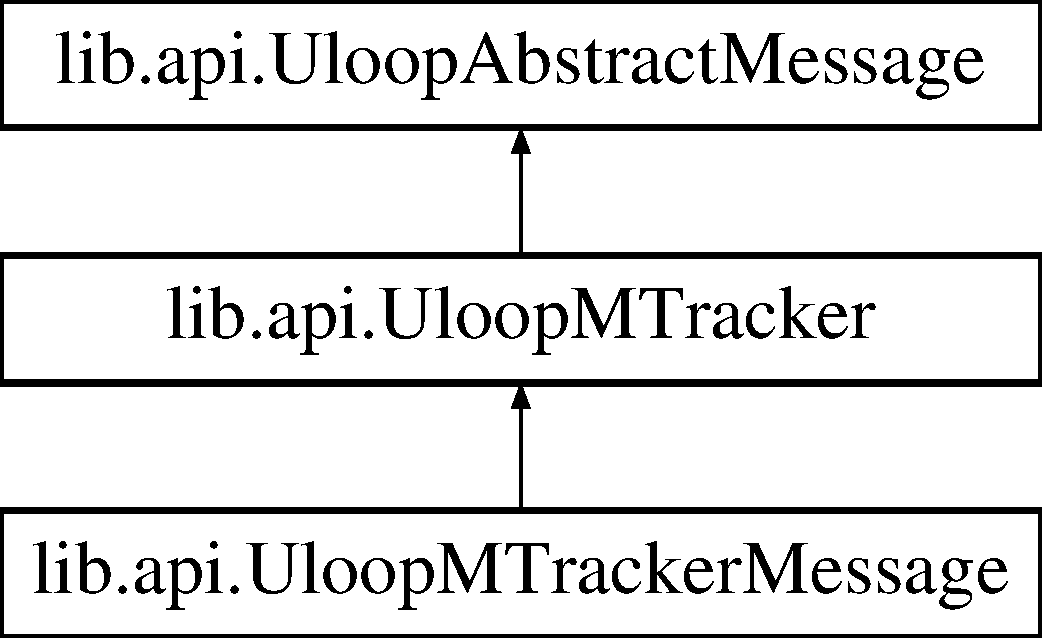
\includegraphics[height=3.000000cm]{classlib_1_1api_1_1UloopMTracker}
\end{center}
\end{figure}
\subsection*{Additional Inherited Members}


The documentation for this class was generated from the following file\+:\begin{DoxyCompactItemize}
\item 
src/lib/api/\hyperlink{UloopMTracker_8java}{Uloop\+M\+Tracker.\+java}\end{DoxyCompactItemize}

\hypertarget{classlib_1_1api_1_1UloopMTrackerMessage}{\section{lib.\+api.\+Uloop\+M\+Tracker\+Message Class Reference}
\label{classlib_1_1api_1_1UloopMTrackerMessage}\index{lib.\+api.\+Uloop\+M\+Tracker\+Message@{lib.\+api.\+Uloop\+M\+Tracker\+Message}}
}
Inheritance diagram for lib.\+api.\+Uloop\+M\+Tracker\+Message\+:\begin{figure}[H]
\begin{center}
\leavevmode
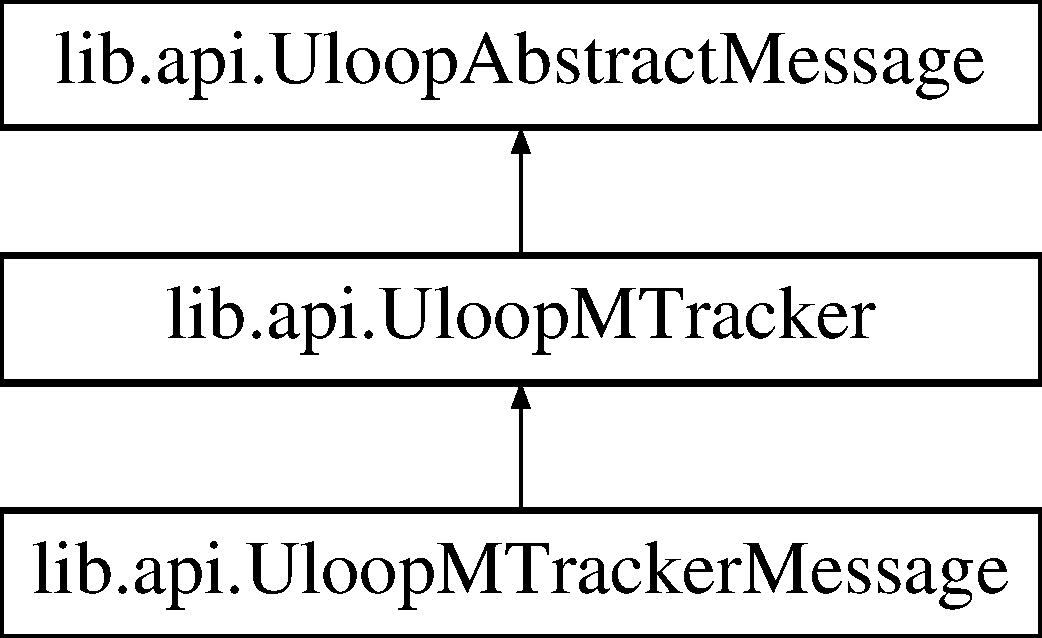
\includegraphics[height=3.000000cm]{classlib_1_1api_1_1UloopMTrackerMessage}
\end{center}
\end{figure}
\subsection*{Classes}
\begin{DoxyCompactItemize}
\item 
class \hyperlink{classlib_1_1api_1_1UloopMTrackerMessage_1_1MTrackerPredictedM}{M\+Tracker\+Predicted\+M}
\end{DoxyCompactItemize}
\subsection*{Public Member Functions}
\begin{DoxyCompactItemize}
\item 
\hyperlink{classlib_1_1api_1_1UloopMTrackerMessage_af2ffccec9a97a071632d90567b5af784}{Uloop\+M\+Tracker\+Message} ()
\item 
void \hyperlink{classlib_1_1api_1_1UloopMTrackerMessage_acae9940756ba963f4c9a703baf738710}{set\+Time\+For\+Next\+Move} (long time)
\item 
void \hyperlink{classlib_1_1api_1_1UloopMTrackerMessage_a2e3de78be834a4e61d5b0f1a3e37eb8d}{set\+Current\+Stationary\+Time} (long time)
\item 
void \hyperlink{classlib_1_1api_1_1UloopMTrackerMessage_a107cb0a2253da877df8d55c2c77c7350}{add\+Next\+Gateway} (\hyperlink{classlib_1_1api_1_1UloopMTrackerMessage_1_1MTrackerPredictedM}{M\+Tracker\+Predicted\+M} next)
\item 
\hyperlink{interfacelib_1_1api_1_1UloopAbstractMessage}{Uloop\+Abstract\+Message} \hyperlink{classlib_1_1api_1_1UloopMTrackerMessage_a3251cbbabd745f22290f334c475d4c97}{decode} (Uloop\+Message ulm)  throws Runtime\+Exception 
\item 
Builder \hyperlink{classlib_1_1api_1_1UloopMTrackerMessage_a9d9ff3e73a53ae13088b52df395de90a}{encode} ()
\item 
void \hyperlink{classlib_1_1api_1_1UloopMTrackerMessage_ad8747254f5616590148266b72b088421}{print} ()
\end{DoxyCompactItemize}
\subsection*{Private Attributes}
\begin{DoxyCompactItemize}
\item 
long \hyperlink{classlib_1_1api_1_1UloopMTrackerMessage_a93952c4aff54e16ddac6099ff2dce1b1}{time\+For\+Next\+Move}
\item 
long \hyperlink{classlib_1_1api_1_1UloopMTrackerMessage_a73fcf2704001aafa37e8f4fe716cefe6}{current\+Stationary\+Time}
\item 
List$<$ \hyperlink{classlib_1_1api_1_1UloopMTrackerMessage_1_1MTrackerPredictedM}{M\+Tracker\+Predicted\+M} $>$ \hyperlink{classlib_1_1api_1_1UloopMTrackerMessage_a4faa2b9d0289c4803f5060f5b76d4d41}{Next\+Gateway\+List}
\end{DoxyCompactItemize}


\subsection{Constructor \& Destructor Documentation}
\hypertarget{classlib_1_1api_1_1UloopMTrackerMessage_af2ffccec9a97a071632d90567b5af784}{\index{lib\+::api\+::\+Uloop\+M\+Tracker\+Message@{lib\+::api\+::\+Uloop\+M\+Tracker\+Message}!Uloop\+M\+Tracker\+Message@{Uloop\+M\+Tracker\+Message}}
\index{Uloop\+M\+Tracker\+Message@{Uloop\+M\+Tracker\+Message}!lib\+::api\+::\+Uloop\+M\+Tracker\+Message@{lib\+::api\+::\+Uloop\+M\+Tracker\+Message}}
\subsubsection[{Uloop\+M\+Tracker\+Message}]{\setlength{\rightskip}{0pt plus 5cm}lib.\+api.\+Uloop\+M\+Tracker\+Message.\+Uloop\+M\+Tracker\+Message (
\begin{DoxyParamCaption}
{}
\end{DoxyParamCaption}
)}}\label{classlib_1_1api_1_1UloopMTrackerMessage_af2ffccec9a97a071632d90567b5af784}


\subsection{Member Function Documentation}
\hypertarget{classlib_1_1api_1_1UloopMTrackerMessage_a107cb0a2253da877df8d55c2c77c7350}{\index{lib\+::api\+::\+Uloop\+M\+Tracker\+Message@{lib\+::api\+::\+Uloop\+M\+Tracker\+Message}!add\+Next\+Gateway@{add\+Next\+Gateway}}
\index{add\+Next\+Gateway@{add\+Next\+Gateway}!lib\+::api\+::\+Uloop\+M\+Tracker\+Message@{lib\+::api\+::\+Uloop\+M\+Tracker\+Message}}
\subsubsection[{add\+Next\+Gateway}]{\setlength{\rightskip}{0pt plus 5cm}void lib.\+api.\+Uloop\+M\+Tracker\+Message.\+add\+Next\+Gateway (
\begin{DoxyParamCaption}
\item[{{\bf M\+Tracker\+Predicted\+M}}]{next}
\end{DoxyParamCaption}
)}}\label{classlib_1_1api_1_1UloopMTrackerMessage_a107cb0a2253da877df8d55c2c77c7350}
\hypertarget{classlib_1_1api_1_1UloopMTrackerMessage_a3251cbbabd745f22290f334c475d4c97}{\index{lib\+::api\+::\+Uloop\+M\+Tracker\+Message@{lib\+::api\+::\+Uloop\+M\+Tracker\+Message}!decode@{decode}}
\index{decode@{decode}!lib\+::api\+::\+Uloop\+M\+Tracker\+Message@{lib\+::api\+::\+Uloop\+M\+Tracker\+Message}}
\subsubsection[{decode}]{\setlength{\rightskip}{0pt plus 5cm}{\bf Uloop\+Abstract\+Message} lib.\+api.\+Uloop\+M\+Tracker\+Message.\+decode (
\begin{DoxyParamCaption}
\item[{Uloop\+Message}]{ulm}
\end{DoxyParamCaption}
) throws Runtime\+Exception}}\label{classlib_1_1api_1_1UloopMTrackerMessage_a3251cbbabd745f22290f334c475d4c97}


Implements \hyperlink{interfacelib_1_1api_1_1UloopAbstractMessage_a1a650d00338402b7d2a5f46575241986}{lib.\+api.\+Uloop\+Abstract\+Message}.

\hypertarget{classlib_1_1api_1_1UloopMTrackerMessage_a9d9ff3e73a53ae13088b52df395de90a}{\index{lib\+::api\+::\+Uloop\+M\+Tracker\+Message@{lib\+::api\+::\+Uloop\+M\+Tracker\+Message}!encode@{encode}}
\index{encode@{encode}!lib\+::api\+::\+Uloop\+M\+Tracker\+Message@{lib\+::api\+::\+Uloop\+M\+Tracker\+Message}}
\subsubsection[{encode}]{\setlength{\rightskip}{0pt plus 5cm}Builder lib.\+api.\+Uloop\+M\+Tracker\+Message.\+encode (
\begin{DoxyParamCaption}
{}
\end{DoxyParamCaption}
)}}\label{classlib_1_1api_1_1UloopMTrackerMessage_a9d9ff3e73a53ae13088b52df395de90a}


Implements \hyperlink{interfacelib_1_1api_1_1UloopAbstractMessage_a00e05a40924dadb7ee429c811628aea3}{lib.\+api.\+Uloop\+Abstract\+Message}.

\hypertarget{classlib_1_1api_1_1UloopMTrackerMessage_ad8747254f5616590148266b72b088421}{\index{lib\+::api\+::\+Uloop\+M\+Tracker\+Message@{lib\+::api\+::\+Uloop\+M\+Tracker\+Message}!print@{print}}
\index{print@{print}!lib\+::api\+::\+Uloop\+M\+Tracker\+Message@{lib\+::api\+::\+Uloop\+M\+Tracker\+Message}}
\subsubsection[{print}]{\setlength{\rightskip}{0pt plus 5cm}void lib.\+api.\+Uloop\+M\+Tracker\+Message.\+print (
\begin{DoxyParamCaption}
{}
\end{DoxyParamCaption}
)}}\label{classlib_1_1api_1_1UloopMTrackerMessage_ad8747254f5616590148266b72b088421}


Implements \hyperlink{interfacelib_1_1api_1_1UloopAbstractMessage_a116bcd258e6e384507888f4a2e2100a9}{lib.\+api.\+Uloop\+Abstract\+Message}.

\hypertarget{classlib_1_1api_1_1UloopMTrackerMessage_a2e3de78be834a4e61d5b0f1a3e37eb8d}{\index{lib\+::api\+::\+Uloop\+M\+Tracker\+Message@{lib\+::api\+::\+Uloop\+M\+Tracker\+Message}!set\+Current\+Stationary\+Time@{set\+Current\+Stationary\+Time}}
\index{set\+Current\+Stationary\+Time@{set\+Current\+Stationary\+Time}!lib\+::api\+::\+Uloop\+M\+Tracker\+Message@{lib\+::api\+::\+Uloop\+M\+Tracker\+Message}}
\subsubsection[{set\+Current\+Stationary\+Time}]{\setlength{\rightskip}{0pt plus 5cm}void lib.\+api.\+Uloop\+M\+Tracker\+Message.\+set\+Current\+Stationary\+Time (
\begin{DoxyParamCaption}
\item[{long}]{time}
\end{DoxyParamCaption}
)}}\label{classlib_1_1api_1_1UloopMTrackerMessage_a2e3de78be834a4e61d5b0f1a3e37eb8d}
\hypertarget{classlib_1_1api_1_1UloopMTrackerMessage_acae9940756ba963f4c9a703baf738710}{\index{lib\+::api\+::\+Uloop\+M\+Tracker\+Message@{lib\+::api\+::\+Uloop\+M\+Tracker\+Message}!set\+Time\+For\+Next\+Move@{set\+Time\+For\+Next\+Move}}
\index{set\+Time\+For\+Next\+Move@{set\+Time\+For\+Next\+Move}!lib\+::api\+::\+Uloop\+M\+Tracker\+Message@{lib\+::api\+::\+Uloop\+M\+Tracker\+Message}}
\subsubsection[{set\+Time\+For\+Next\+Move}]{\setlength{\rightskip}{0pt plus 5cm}void lib.\+api.\+Uloop\+M\+Tracker\+Message.\+set\+Time\+For\+Next\+Move (
\begin{DoxyParamCaption}
\item[{long}]{time}
\end{DoxyParamCaption}
)}}\label{classlib_1_1api_1_1UloopMTrackerMessage_acae9940756ba963f4c9a703baf738710}


\subsection{Member Data Documentation}
\hypertarget{classlib_1_1api_1_1UloopMTrackerMessage_a73fcf2704001aafa37e8f4fe716cefe6}{\index{lib\+::api\+::\+Uloop\+M\+Tracker\+Message@{lib\+::api\+::\+Uloop\+M\+Tracker\+Message}!current\+Stationary\+Time@{current\+Stationary\+Time}}
\index{current\+Stationary\+Time@{current\+Stationary\+Time}!lib\+::api\+::\+Uloop\+M\+Tracker\+Message@{lib\+::api\+::\+Uloop\+M\+Tracker\+Message}}
\subsubsection[{current\+Stationary\+Time}]{\setlength{\rightskip}{0pt plus 5cm}long lib.\+api.\+Uloop\+M\+Tracker\+Message.\+current\+Stationary\+Time\hspace{0.3cm}{\ttfamily [private]}}}\label{classlib_1_1api_1_1UloopMTrackerMessage_a73fcf2704001aafa37e8f4fe716cefe6}
\hypertarget{classlib_1_1api_1_1UloopMTrackerMessage_a4faa2b9d0289c4803f5060f5b76d4d41}{\index{lib\+::api\+::\+Uloop\+M\+Tracker\+Message@{lib\+::api\+::\+Uloop\+M\+Tracker\+Message}!Next\+Gateway\+List@{Next\+Gateway\+List}}
\index{Next\+Gateway\+List@{Next\+Gateway\+List}!lib\+::api\+::\+Uloop\+M\+Tracker\+Message@{lib\+::api\+::\+Uloop\+M\+Tracker\+Message}}
\subsubsection[{Next\+Gateway\+List}]{\setlength{\rightskip}{0pt plus 5cm}List$<${\bf M\+Tracker\+Predicted\+M}$>$ lib.\+api.\+Uloop\+M\+Tracker\+Message.\+Next\+Gateway\+List\hspace{0.3cm}{\ttfamily [private]}}}\label{classlib_1_1api_1_1UloopMTrackerMessage_a4faa2b9d0289c4803f5060f5b76d4d41}
\hypertarget{classlib_1_1api_1_1UloopMTrackerMessage_a93952c4aff54e16ddac6099ff2dce1b1}{\index{lib\+::api\+::\+Uloop\+M\+Tracker\+Message@{lib\+::api\+::\+Uloop\+M\+Tracker\+Message}!time\+For\+Next\+Move@{time\+For\+Next\+Move}}
\index{time\+For\+Next\+Move@{time\+For\+Next\+Move}!lib\+::api\+::\+Uloop\+M\+Tracker\+Message@{lib\+::api\+::\+Uloop\+M\+Tracker\+Message}}
\subsubsection[{time\+For\+Next\+Move}]{\setlength{\rightskip}{0pt plus 5cm}long lib.\+api.\+Uloop\+M\+Tracker\+Message.\+time\+For\+Next\+Move\hspace{0.3cm}{\ttfamily [private]}}}\label{classlib_1_1api_1_1UloopMTrackerMessage_a93952c4aff54e16ddac6099ff2dce1b1}


The documentation for this class was generated from the following file\+:\begin{DoxyCompactItemize}
\item 
src/lib/api/\hyperlink{UloopMTrackerMessage_8java}{Uloop\+M\+Tracker\+Message.\+java}\end{DoxyCompactItemize}

\hypertarget{classlib_1_1api_1_1UloopService}{\section{lib.\+api.\+Uloop\+Service Class Reference}
\label{classlib_1_1api_1_1UloopService}\index{lib.\+api.\+Uloop\+Service@{lib.\+api.\+Uloop\+Service}}
}
Inheritance diagram for lib.\+api.\+Uloop\+Service\+:\begin{figure}[H]
\begin{center}
\leavevmode
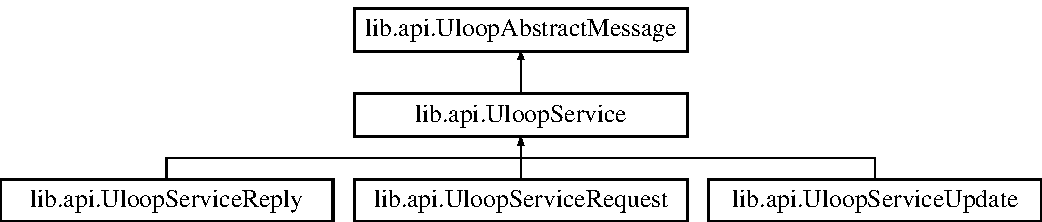
\includegraphics[height=2.978723cm]{classlib_1_1api_1_1UloopService}
\end{center}
\end{figure}
\subsection*{Additional Inherited Members}


The documentation for this class was generated from the following file\+:\begin{DoxyCompactItemize}
\item 
src/lib/api/\hyperlink{UloopService_8java}{Uloop\+Service.\+java}\end{DoxyCompactItemize}

\hypertarget{classlib_1_1api_1_1UloopServiceReply}{\section{lib.\+api.\+Uloop\+Service\+Reply Class Reference}
\label{classlib_1_1api_1_1UloopServiceReply}\index{lib.\+api.\+Uloop\+Service\+Reply@{lib.\+api.\+Uloop\+Service\+Reply}}
}
Inheritance diagram for lib.\+api.\+Uloop\+Service\+Reply\+:\begin{figure}[H]
\begin{center}
\leavevmode
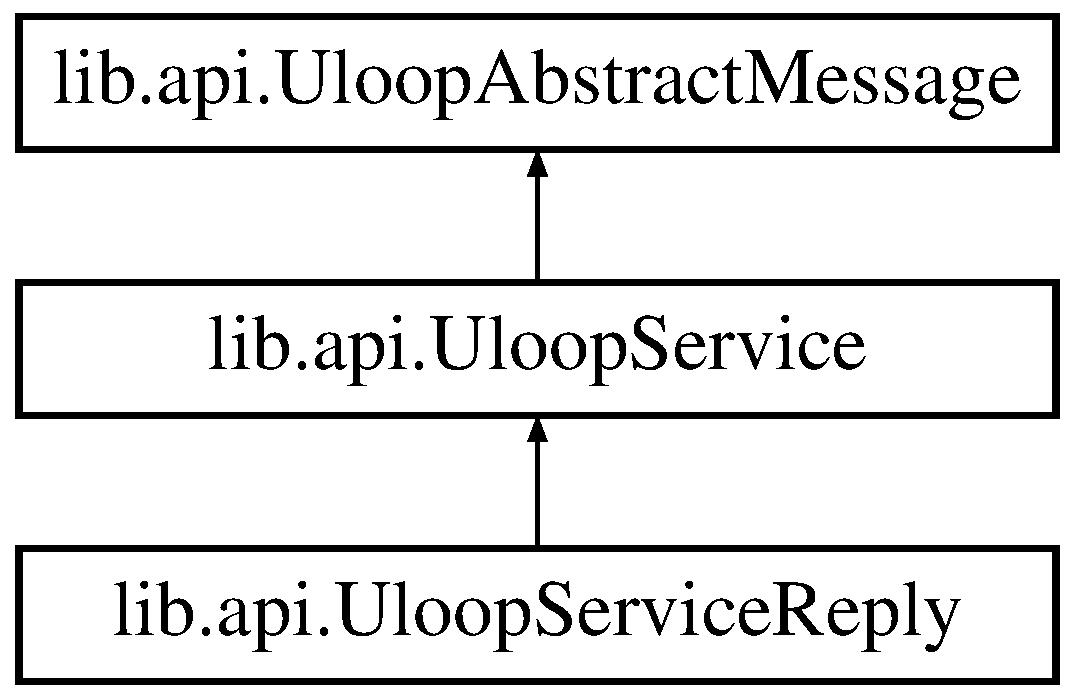
\includegraphics[height=3.000000cm]{classlib_1_1api_1_1UloopServiceReply}
\end{center}
\end{figure}
\subsection*{Public Member Functions}
\begin{DoxyCompactItemize}
\item 
\hyperlink{classlib_1_1api_1_1UloopServiceReply_ac3acd1326ef054d7f7e9d9c6aad50198}{Uloop\+Service\+Reply} ()
\item 
\hyperlink{classlib_1_1api_1_1UloopServiceReply_ac3b222046392ac4e530b0b72a5f39dc0}{Uloop\+Service\+Reply} (boolean \hyperlink{classlib_1_1api_1_1UloopServiceReply_a9fe9ecb4fca6ed06fe77c70adf42be11}{authorization}, double \hyperlink{classlib_1_1api_1_1UloopServiceReply_a5ad9fd3217140d290e9704e55dd6dc3b}{trust})
\item 
void \hyperlink{classlib_1_1api_1_1UloopServiceReply_ac194f67f052d8c8722a1a92859be49c0}{set\+Authorization} (boolean \hyperlink{classlib_1_1api_1_1UloopServiceReply_a9fe9ecb4fca6ed06fe77c70adf42be11}{authorization})
\item 
void \hyperlink{classlib_1_1api_1_1UloopServiceReply_a84259060d5524cc5e91f63700105785e}{set\+Crypto\+I\+D} (\hyperlink{classlib_1_1api_1_1CryptoID}{Crypto\+I\+D} cid)
\item 
void \hyperlink{classlib_1_1api_1_1UloopServiceReply_a7a2e472da008b2b8a513ec8f19fb50eb}{set\+Trust} (double \hyperlink{classlib_1_1api_1_1UloopServiceReply_a5ad9fd3217140d290e9704e55dd6dc3b}{trust})
\item 
\hyperlink{interfacelib_1_1api_1_1UloopAbstractMessage}{Uloop\+Abstract\+Message} \hyperlink{classlib_1_1api_1_1UloopServiceReply_a944ecbe5d5a40e6ae48ee884063f5c1d}{decode} (Uloop\+Message ulm)  throws Runtime\+Exception 
\item 
Builder \hyperlink{classlib_1_1api_1_1UloopServiceReply_a0ca29eaf04dce5493607e010b73f77d4}{encode} ()
\item 
void \hyperlink{classlib_1_1api_1_1UloopServiceReply_a825bbcd3250cc8ac980f3eda449c482f}{print} ()
\end{DoxyCompactItemize}
\subsection*{Private Attributes}
\begin{DoxyCompactItemize}
\item 
boolean \hyperlink{classlib_1_1api_1_1UloopServiceReply_a9fe9ecb4fca6ed06fe77c70adf42be11}{authorization}
\item 
double \hyperlink{classlib_1_1api_1_1UloopServiceReply_a5ad9fd3217140d290e9704e55dd6dc3b}{trust}
\item 
\hyperlink{classlib_1_1api_1_1CryptoID}{Crypto\+I\+D} \hyperlink{classlib_1_1api_1_1UloopServiceReply_a3be01631c077de8781d55e2f2ea09440}{cryptoid}
\end{DoxyCompactItemize}


\subsection{Constructor \& Destructor Documentation}
\hypertarget{classlib_1_1api_1_1UloopServiceReply_ac3acd1326ef054d7f7e9d9c6aad50198}{\index{lib\+::api\+::\+Uloop\+Service\+Reply@{lib\+::api\+::\+Uloop\+Service\+Reply}!Uloop\+Service\+Reply@{Uloop\+Service\+Reply}}
\index{Uloop\+Service\+Reply@{Uloop\+Service\+Reply}!lib\+::api\+::\+Uloop\+Service\+Reply@{lib\+::api\+::\+Uloop\+Service\+Reply}}
\subsubsection[{Uloop\+Service\+Reply}]{\setlength{\rightskip}{0pt plus 5cm}lib.\+api.\+Uloop\+Service\+Reply.\+Uloop\+Service\+Reply (
\begin{DoxyParamCaption}
{}
\end{DoxyParamCaption}
)}}\label{classlib_1_1api_1_1UloopServiceReply_ac3acd1326ef054d7f7e9d9c6aad50198}
\hypertarget{classlib_1_1api_1_1UloopServiceReply_ac3b222046392ac4e530b0b72a5f39dc0}{\index{lib\+::api\+::\+Uloop\+Service\+Reply@{lib\+::api\+::\+Uloop\+Service\+Reply}!Uloop\+Service\+Reply@{Uloop\+Service\+Reply}}
\index{Uloop\+Service\+Reply@{Uloop\+Service\+Reply}!lib\+::api\+::\+Uloop\+Service\+Reply@{lib\+::api\+::\+Uloop\+Service\+Reply}}
\subsubsection[{Uloop\+Service\+Reply}]{\setlength{\rightskip}{0pt plus 5cm}lib.\+api.\+Uloop\+Service\+Reply.\+Uloop\+Service\+Reply (
\begin{DoxyParamCaption}
\item[{boolean}]{authorization, }
\item[{double}]{trust}
\end{DoxyParamCaption}
)}}\label{classlib_1_1api_1_1UloopServiceReply_ac3b222046392ac4e530b0b72a5f39dc0}


\subsection{Member Function Documentation}
\hypertarget{classlib_1_1api_1_1UloopServiceReply_a944ecbe5d5a40e6ae48ee884063f5c1d}{\index{lib\+::api\+::\+Uloop\+Service\+Reply@{lib\+::api\+::\+Uloop\+Service\+Reply}!decode@{decode}}
\index{decode@{decode}!lib\+::api\+::\+Uloop\+Service\+Reply@{lib\+::api\+::\+Uloop\+Service\+Reply}}
\subsubsection[{decode}]{\setlength{\rightskip}{0pt plus 5cm}{\bf Uloop\+Abstract\+Message} lib.\+api.\+Uloop\+Service\+Reply.\+decode (
\begin{DoxyParamCaption}
\item[{Uloop\+Message}]{ulm}
\end{DoxyParamCaption}
) throws Runtime\+Exception}}\label{classlib_1_1api_1_1UloopServiceReply_a944ecbe5d5a40e6ae48ee884063f5c1d}


Implements \hyperlink{interfacelib_1_1api_1_1UloopAbstractMessage_a1a650d00338402b7d2a5f46575241986}{lib.\+api.\+Uloop\+Abstract\+Message}.

\hypertarget{classlib_1_1api_1_1UloopServiceReply_a0ca29eaf04dce5493607e010b73f77d4}{\index{lib\+::api\+::\+Uloop\+Service\+Reply@{lib\+::api\+::\+Uloop\+Service\+Reply}!encode@{encode}}
\index{encode@{encode}!lib\+::api\+::\+Uloop\+Service\+Reply@{lib\+::api\+::\+Uloop\+Service\+Reply}}
\subsubsection[{encode}]{\setlength{\rightskip}{0pt plus 5cm}Builder lib.\+api.\+Uloop\+Service\+Reply.\+encode (
\begin{DoxyParamCaption}
{}
\end{DoxyParamCaption}
)}}\label{classlib_1_1api_1_1UloopServiceReply_a0ca29eaf04dce5493607e010b73f77d4}


Implements \hyperlink{interfacelib_1_1api_1_1UloopAbstractMessage_a00e05a40924dadb7ee429c811628aea3}{lib.\+api.\+Uloop\+Abstract\+Message}.

\hypertarget{classlib_1_1api_1_1UloopServiceReply_a825bbcd3250cc8ac980f3eda449c482f}{\index{lib\+::api\+::\+Uloop\+Service\+Reply@{lib\+::api\+::\+Uloop\+Service\+Reply}!print@{print}}
\index{print@{print}!lib\+::api\+::\+Uloop\+Service\+Reply@{lib\+::api\+::\+Uloop\+Service\+Reply}}
\subsubsection[{print}]{\setlength{\rightskip}{0pt plus 5cm}void lib.\+api.\+Uloop\+Service\+Reply.\+print (
\begin{DoxyParamCaption}
{}
\end{DoxyParamCaption}
)}}\label{classlib_1_1api_1_1UloopServiceReply_a825bbcd3250cc8ac980f3eda449c482f}


Implements \hyperlink{interfacelib_1_1api_1_1UloopAbstractMessage_a116bcd258e6e384507888f4a2e2100a9}{lib.\+api.\+Uloop\+Abstract\+Message}.

\hypertarget{classlib_1_1api_1_1UloopServiceReply_ac194f67f052d8c8722a1a92859be49c0}{\index{lib\+::api\+::\+Uloop\+Service\+Reply@{lib\+::api\+::\+Uloop\+Service\+Reply}!set\+Authorization@{set\+Authorization}}
\index{set\+Authorization@{set\+Authorization}!lib\+::api\+::\+Uloop\+Service\+Reply@{lib\+::api\+::\+Uloop\+Service\+Reply}}
\subsubsection[{set\+Authorization}]{\setlength{\rightskip}{0pt plus 5cm}void lib.\+api.\+Uloop\+Service\+Reply.\+set\+Authorization (
\begin{DoxyParamCaption}
\item[{boolean}]{authorization}
\end{DoxyParamCaption}
)}}\label{classlib_1_1api_1_1UloopServiceReply_ac194f67f052d8c8722a1a92859be49c0}
\hypertarget{classlib_1_1api_1_1UloopServiceReply_a84259060d5524cc5e91f63700105785e}{\index{lib\+::api\+::\+Uloop\+Service\+Reply@{lib\+::api\+::\+Uloop\+Service\+Reply}!set\+Crypto\+I\+D@{set\+Crypto\+I\+D}}
\index{set\+Crypto\+I\+D@{set\+Crypto\+I\+D}!lib\+::api\+::\+Uloop\+Service\+Reply@{lib\+::api\+::\+Uloop\+Service\+Reply}}
\subsubsection[{set\+Crypto\+I\+D}]{\setlength{\rightskip}{0pt plus 5cm}void lib.\+api.\+Uloop\+Service\+Reply.\+set\+Crypto\+I\+D (
\begin{DoxyParamCaption}
\item[{{\bf Crypto\+I\+D}}]{cid}
\end{DoxyParamCaption}
)}}\label{classlib_1_1api_1_1UloopServiceReply_a84259060d5524cc5e91f63700105785e}
\hypertarget{classlib_1_1api_1_1UloopServiceReply_a7a2e472da008b2b8a513ec8f19fb50eb}{\index{lib\+::api\+::\+Uloop\+Service\+Reply@{lib\+::api\+::\+Uloop\+Service\+Reply}!set\+Trust@{set\+Trust}}
\index{set\+Trust@{set\+Trust}!lib\+::api\+::\+Uloop\+Service\+Reply@{lib\+::api\+::\+Uloop\+Service\+Reply}}
\subsubsection[{set\+Trust}]{\setlength{\rightskip}{0pt plus 5cm}void lib.\+api.\+Uloop\+Service\+Reply.\+set\+Trust (
\begin{DoxyParamCaption}
\item[{double}]{trust}
\end{DoxyParamCaption}
)}}\label{classlib_1_1api_1_1UloopServiceReply_a7a2e472da008b2b8a513ec8f19fb50eb}


\subsection{Member Data Documentation}
\hypertarget{classlib_1_1api_1_1UloopServiceReply_a9fe9ecb4fca6ed06fe77c70adf42be11}{\index{lib\+::api\+::\+Uloop\+Service\+Reply@{lib\+::api\+::\+Uloop\+Service\+Reply}!authorization@{authorization}}
\index{authorization@{authorization}!lib\+::api\+::\+Uloop\+Service\+Reply@{lib\+::api\+::\+Uloop\+Service\+Reply}}
\subsubsection[{authorization}]{\setlength{\rightskip}{0pt plus 5cm}boolean lib.\+api.\+Uloop\+Service\+Reply.\+authorization\hspace{0.3cm}{\ttfamily [private]}}}\label{classlib_1_1api_1_1UloopServiceReply_a9fe9ecb4fca6ed06fe77c70adf42be11}
\hypertarget{classlib_1_1api_1_1UloopServiceReply_a3be01631c077de8781d55e2f2ea09440}{\index{lib\+::api\+::\+Uloop\+Service\+Reply@{lib\+::api\+::\+Uloop\+Service\+Reply}!cryptoid@{cryptoid}}
\index{cryptoid@{cryptoid}!lib\+::api\+::\+Uloop\+Service\+Reply@{lib\+::api\+::\+Uloop\+Service\+Reply}}
\subsubsection[{cryptoid}]{\setlength{\rightskip}{0pt plus 5cm}{\bf Crypto\+I\+D} lib.\+api.\+Uloop\+Service\+Reply.\+cryptoid\hspace{0.3cm}{\ttfamily [private]}}}\label{classlib_1_1api_1_1UloopServiceReply_a3be01631c077de8781d55e2f2ea09440}
\hypertarget{classlib_1_1api_1_1UloopServiceReply_a5ad9fd3217140d290e9704e55dd6dc3b}{\index{lib\+::api\+::\+Uloop\+Service\+Reply@{lib\+::api\+::\+Uloop\+Service\+Reply}!trust@{trust}}
\index{trust@{trust}!lib\+::api\+::\+Uloop\+Service\+Reply@{lib\+::api\+::\+Uloop\+Service\+Reply}}
\subsubsection[{trust}]{\setlength{\rightskip}{0pt plus 5cm}double lib.\+api.\+Uloop\+Service\+Reply.\+trust\hspace{0.3cm}{\ttfamily [private]}}}\label{classlib_1_1api_1_1UloopServiceReply_a5ad9fd3217140d290e9704e55dd6dc3b}


The documentation for this class was generated from the following file\+:\begin{DoxyCompactItemize}
\item 
src/lib/api/\hyperlink{UloopServiceReply_8java}{Uloop\+Service\+Reply.\+java}\end{DoxyCompactItemize}

\hypertarget{classlib_1_1api_1_1UloopServiceRequest}{\section{lib.\+api.\+Uloop\+Service\+Request Class Reference}
\label{classlib_1_1api_1_1UloopServiceRequest}\index{lib.\+api.\+Uloop\+Service\+Request@{lib.\+api.\+Uloop\+Service\+Request}}
}
Inheritance diagram for lib.\+api.\+Uloop\+Service\+Request\+:\begin{figure}[H]
\begin{center}
\leavevmode
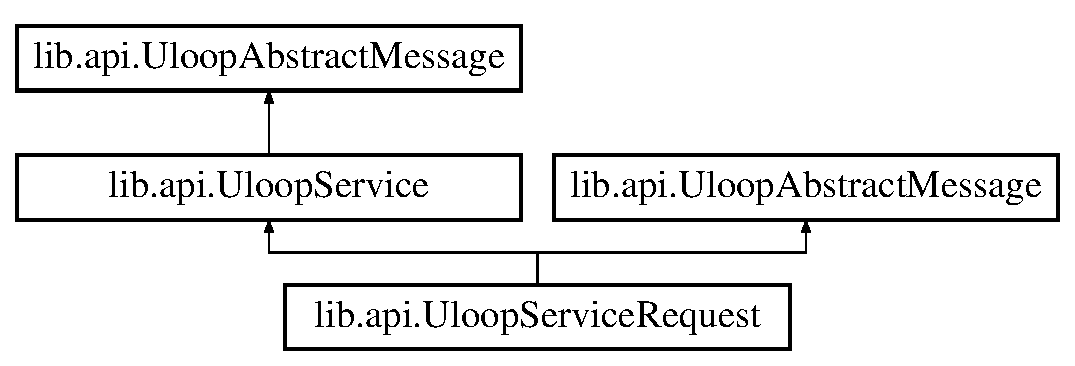
\includegraphics[height=3.000000cm]{classlib_1_1api_1_1UloopServiceRequest}
\end{center}
\end{figure}
\subsection*{Public Member Functions}
\begin{DoxyCompactItemize}
\item 
\hyperlink{classlib_1_1api_1_1UloopServiceRequest_a7efc91eb413b65384b379dddbbdc8166}{Uloop\+Service\+Request} ()
\item 
\hyperlink{classlib_1_1api_1_1UloopServiceRequest_ac7928f753be32f759214773e9eb9d2cf}{Uloop\+Service\+Request} (\hyperlink{classlib_1_1api_1_1CryptoID}{Crypto\+I\+D} \hyperlink{classlib_1_1api_1_1UloopServiceRequest_affac2350c8b10ac404fa381f4ee93cb0}{cryptoid})
\item 
void \hyperlink{classlib_1_1api_1_1UloopServiceRequest_a951ef79492864bb953168d14666e7dfc}{set\+Username} (byte\mbox{[}$\,$\mbox{]}\hyperlink{classlib_1_1api_1_1UloopServiceRequest_a8a929330893f001347b4df81927edd4c}{username})
\item 
void \hyperlink{classlib_1_1api_1_1UloopServiceRequest_a591c6f2cfe2218c889ea7c81174d1d55}{set\+Password} (byte\mbox{[}$\,$\mbox{]}\hyperlink{classlib_1_1api_1_1UloopServiceRequest_a0c23579473c23dbc9411c2c444af4714}{password})
\item 
void \hyperlink{classlib_1_1api_1_1UloopServiceRequest_adf89fa97301f24dae9d16580f2170903}{set\+Promise\+Of\+Payment} (byte\mbox{[}$\,$\mbox{]}\hyperlink{classlib_1_1api_1_1UloopServiceRequest_a1a1cd5bf12daafcaea1a016b717cc719}{promise\+\_\+of\+\_\+payment})
\item 
void \hyperlink{classlib_1_1api_1_1UloopServiceRequest_a9b40ab10532f92bb429758296a474def}{set\+Tokens} (double \hyperlink{classlib_1_1api_1_1UloopServiceRequest_a768929461a7fbf8cfabb565a00c44d64}{tokens})
\item 
void \hyperlink{classlib_1_1api_1_1UloopServiceRequest_affcac88524bf65f1ef0301b0b20f340a}{set\+Crypto\+I\+D} (\hyperlink{classlib_1_1api_1_1CryptoID}{Crypto\+I\+D} \hyperlink{classlib_1_1api_1_1UloopServiceRequest_affac2350c8b10ac404fa381f4ee93cb0}{cryptoid})
\item 
\hyperlink{interfacelib_1_1api_1_1UloopAbstractMessage}{Uloop\+Abstract\+Message} \hyperlink{classlib_1_1api_1_1UloopServiceRequest_a4a8a64d824425f1d326f3be82115ccf2}{decode} (Uloop\+Message ulm)  throws Runtime\+Exception
\item 
Uloop\+Message.\+Builder \hyperlink{classlib_1_1api_1_1UloopServiceRequest_a13409dd756188327c2885eda6f9a8b17}{encode} ()
\item 
\hyperlink{classlib_1_1api_1_1CryptoID}{Crypto\+I\+D} \hyperlink{classlib_1_1api_1_1UloopServiceRequest_a3bad2fd6dc96c07cf6ac6b076b597a64}{get\+Cryptoid} ()
\item 
void \hyperlink{classlib_1_1api_1_1UloopServiceRequest_a297690e00aed1f79499de2c9095fe52c}{print} ()
\end{DoxyCompactItemize}
\subsection*{Private Attributes}
\begin{DoxyCompactItemize}
\item 
\hyperlink{classlib_1_1api_1_1CryptoID}{Crypto\+I\+D} \hyperlink{classlib_1_1api_1_1UloopServiceRequest_affac2350c8b10ac404fa381f4ee93cb0}{cryptoid}
\item 
byte\mbox{[}$\,$\mbox{]} \hyperlink{classlib_1_1api_1_1UloopServiceRequest_a8a929330893f001347b4df81927edd4c}{username}
\item 
byte\mbox{[}$\,$\mbox{]} \hyperlink{classlib_1_1api_1_1UloopServiceRequest_a0c23579473c23dbc9411c2c444af4714}{password}
\item 
double \hyperlink{classlib_1_1api_1_1UloopServiceRequest_a768929461a7fbf8cfabb565a00c44d64}{tokens}
\item 
byte\mbox{[}$\,$\mbox{]} \hyperlink{classlib_1_1api_1_1UloopServiceRequest_a1a1cd5bf12daafcaea1a016b717cc719}{promise\+\_\+of\+\_\+payment}
\end{DoxyCompactItemize}


\subsection{Constructor \& Destructor Documentation}
\hypertarget{classlib_1_1api_1_1UloopServiceRequest_a7efc91eb413b65384b379dddbbdc8166}{\index{lib\+::api\+::\+Uloop\+Service\+Request@{lib\+::api\+::\+Uloop\+Service\+Request}!Uloop\+Service\+Request@{Uloop\+Service\+Request}}
\index{Uloop\+Service\+Request@{Uloop\+Service\+Request}!lib\+::api\+::\+Uloop\+Service\+Request@{lib\+::api\+::\+Uloop\+Service\+Request}}
\subsubsection[{Uloop\+Service\+Request}]{\setlength{\rightskip}{0pt plus 5cm}lib.\+api.\+Uloop\+Service\+Request.\+Uloop\+Service\+Request (
\begin{DoxyParamCaption}
{}
\end{DoxyParamCaption}
)}}\label{classlib_1_1api_1_1UloopServiceRequest_a7efc91eb413b65384b379dddbbdc8166}
\hypertarget{classlib_1_1api_1_1UloopServiceRequest_ac7928f753be32f759214773e9eb9d2cf}{\index{lib\+::api\+::\+Uloop\+Service\+Request@{lib\+::api\+::\+Uloop\+Service\+Request}!Uloop\+Service\+Request@{Uloop\+Service\+Request}}
\index{Uloop\+Service\+Request@{Uloop\+Service\+Request}!lib\+::api\+::\+Uloop\+Service\+Request@{lib\+::api\+::\+Uloop\+Service\+Request}}
\subsubsection[{Uloop\+Service\+Request}]{\setlength{\rightskip}{0pt plus 5cm}lib.\+api.\+Uloop\+Service\+Request.\+Uloop\+Service\+Request (
\begin{DoxyParamCaption}
\item[{{\bf Crypto\+I\+D}}]{cryptoid}
\end{DoxyParamCaption}
)}}\label{classlib_1_1api_1_1UloopServiceRequest_ac7928f753be32f759214773e9eb9d2cf}


\subsection{Member Function Documentation}
\hypertarget{classlib_1_1api_1_1UloopServiceRequest_a4a8a64d824425f1d326f3be82115ccf2}{\index{lib\+::api\+::\+Uloop\+Service\+Request@{lib\+::api\+::\+Uloop\+Service\+Request}!decode@{decode}}
\index{decode@{decode}!lib\+::api\+::\+Uloop\+Service\+Request@{lib\+::api\+::\+Uloop\+Service\+Request}}
\subsubsection[{decode}]{\setlength{\rightskip}{0pt plus 5cm}{\bf Uloop\+Abstract\+Message} lib.\+api.\+Uloop\+Service\+Request.\+decode (
\begin{DoxyParamCaption}
\item[{Uloop\+Message}]{ulm}
\end{DoxyParamCaption}
) throws Runtime\+Exception}}\label{classlib_1_1api_1_1UloopServiceRequest_a4a8a64d824425f1d326f3be82115ccf2}


Implements \hyperlink{interfacelib_1_1api_1_1UloopAbstractMessage_a1a650d00338402b7d2a5f46575241986}{lib.\+api.\+Uloop\+Abstract\+Message}.

\hypertarget{classlib_1_1api_1_1UloopServiceRequest_a13409dd756188327c2885eda6f9a8b17}{\index{lib\+::api\+::\+Uloop\+Service\+Request@{lib\+::api\+::\+Uloop\+Service\+Request}!encode@{encode}}
\index{encode@{encode}!lib\+::api\+::\+Uloop\+Service\+Request@{lib\+::api\+::\+Uloop\+Service\+Request}}
\subsubsection[{encode}]{\setlength{\rightskip}{0pt plus 5cm}Uloop\+Message.\+Builder lib.\+api.\+Uloop\+Service\+Request.\+encode (
\begin{DoxyParamCaption}
{}
\end{DoxyParamCaption}
)}}\label{classlib_1_1api_1_1UloopServiceRequest_a13409dd756188327c2885eda6f9a8b17}


Implements \hyperlink{interfacelib_1_1api_1_1UloopAbstractMessage_a00e05a40924dadb7ee429c811628aea3}{lib.\+api.\+Uloop\+Abstract\+Message}.

\hypertarget{classlib_1_1api_1_1UloopServiceRequest_a3bad2fd6dc96c07cf6ac6b076b597a64}{\index{lib\+::api\+::\+Uloop\+Service\+Request@{lib\+::api\+::\+Uloop\+Service\+Request}!get\+Cryptoid@{get\+Cryptoid}}
\index{get\+Cryptoid@{get\+Cryptoid}!lib\+::api\+::\+Uloop\+Service\+Request@{lib\+::api\+::\+Uloop\+Service\+Request}}
\subsubsection[{get\+Cryptoid}]{\setlength{\rightskip}{0pt plus 5cm}{\bf Crypto\+I\+D} lib.\+api.\+Uloop\+Service\+Request.\+get\+Cryptoid (
\begin{DoxyParamCaption}
{}
\end{DoxyParamCaption}
)}}\label{classlib_1_1api_1_1UloopServiceRequest_a3bad2fd6dc96c07cf6ac6b076b597a64}
\hypertarget{classlib_1_1api_1_1UloopServiceRequest_a297690e00aed1f79499de2c9095fe52c}{\index{lib\+::api\+::\+Uloop\+Service\+Request@{lib\+::api\+::\+Uloop\+Service\+Request}!print@{print}}
\index{print@{print}!lib\+::api\+::\+Uloop\+Service\+Request@{lib\+::api\+::\+Uloop\+Service\+Request}}
\subsubsection[{print}]{\setlength{\rightskip}{0pt plus 5cm}void lib.\+api.\+Uloop\+Service\+Request.\+print (
\begin{DoxyParamCaption}
{}
\end{DoxyParamCaption}
)}}\label{classlib_1_1api_1_1UloopServiceRequest_a297690e00aed1f79499de2c9095fe52c}


Implements \hyperlink{interfacelib_1_1api_1_1UloopAbstractMessage_a116bcd258e6e384507888f4a2e2100a9}{lib.\+api.\+Uloop\+Abstract\+Message}.

\hypertarget{classlib_1_1api_1_1UloopServiceRequest_affcac88524bf65f1ef0301b0b20f340a}{\index{lib\+::api\+::\+Uloop\+Service\+Request@{lib\+::api\+::\+Uloop\+Service\+Request}!set\+Crypto\+I\+D@{set\+Crypto\+I\+D}}
\index{set\+Crypto\+I\+D@{set\+Crypto\+I\+D}!lib\+::api\+::\+Uloop\+Service\+Request@{lib\+::api\+::\+Uloop\+Service\+Request}}
\subsubsection[{set\+Crypto\+I\+D}]{\setlength{\rightskip}{0pt plus 5cm}void lib.\+api.\+Uloop\+Service\+Request.\+set\+Crypto\+I\+D (
\begin{DoxyParamCaption}
\item[{{\bf Crypto\+I\+D}}]{cryptoid}
\end{DoxyParamCaption}
)}}\label{classlib_1_1api_1_1UloopServiceRequest_affcac88524bf65f1ef0301b0b20f340a}
\hypertarget{classlib_1_1api_1_1UloopServiceRequest_a591c6f2cfe2218c889ea7c81174d1d55}{\index{lib\+::api\+::\+Uloop\+Service\+Request@{lib\+::api\+::\+Uloop\+Service\+Request}!set\+Password@{set\+Password}}
\index{set\+Password@{set\+Password}!lib\+::api\+::\+Uloop\+Service\+Request@{lib\+::api\+::\+Uloop\+Service\+Request}}
\subsubsection[{set\+Password}]{\setlength{\rightskip}{0pt plus 5cm}void lib.\+api.\+Uloop\+Service\+Request.\+set\+Password (
\begin{DoxyParamCaption}
\item[{byte\mbox{[}$\,$\mbox{]}}]{password}
\end{DoxyParamCaption}
)}}\label{classlib_1_1api_1_1UloopServiceRequest_a591c6f2cfe2218c889ea7c81174d1d55}
\hypertarget{classlib_1_1api_1_1UloopServiceRequest_adf89fa97301f24dae9d16580f2170903}{\index{lib\+::api\+::\+Uloop\+Service\+Request@{lib\+::api\+::\+Uloop\+Service\+Request}!set\+Promise\+Of\+Payment@{set\+Promise\+Of\+Payment}}
\index{set\+Promise\+Of\+Payment@{set\+Promise\+Of\+Payment}!lib\+::api\+::\+Uloop\+Service\+Request@{lib\+::api\+::\+Uloop\+Service\+Request}}
\subsubsection[{set\+Promise\+Of\+Payment}]{\setlength{\rightskip}{0pt plus 5cm}void lib.\+api.\+Uloop\+Service\+Request.\+set\+Promise\+Of\+Payment (
\begin{DoxyParamCaption}
\item[{byte\mbox{[}$\,$\mbox{]}}]{promise\+\_\+of\+\_\+payment}
\end{DoxyParamCaption}
)}}\label{classlib_1_1api_1_1UloopServiceRequest_adf89fa97301f24dae9d16580f2170903}
\hypertarget{classlib_1_1api_1_1UloopServiceRequest_a9b40ab10532f92bb429758296a474def}{\index{lib\+::api\+::\+Uloop\+Service\+Request@{lib\+::api\+::\+Uloop\+Service\+Request}!set\+Tokens@{set\+Tokens}}
\index{set\+Tokens@{set\+Tokens}!lib\+::api\+::\+Uloop\+Service\+Request@{lib\+::api\+::\+Uloop\+Service\+Request}}
\subsubsection[{set\+Tokens}]{\setlength{\rightskip}{0pt plus 5cm}void lib.\+api.\+Uloop\+Service\+Request.\+set\+Tokens (
\begin{DoxyParamCaption}
\item[{double}]{tokens}
\end{DoxyParamCaption}
)}}\label{classlib_1_1api_1_1UloopServiceRequest_a9b40ab10532f92bb429758296a474def}
\hypertarget{classlib_1_1api_1_1UloopServiceRequest_a951ef79492864bb953168d14666e7dfc}{\index{lib\+::api\+::\+Uloop\+Service\+Request@{lib\+::api\+::\+Uloop\+Service\+Request}!set\+Username@{set\+Username}}
\index{set\+Username@{set\+Username}!lib\+::api\+::\+Uloop\+Service\+Request@{lib\+::api\+::\+Uloop\+Service\+Request}}
\subsubsection[{set\+Username}]{\setlength{\rightskip}{0pt plus 5cm}void lib.\+api.\+Uloop\+Service\+Request.\+set\+Username (
\begin{DoxyParamCaption}
\item[{byte\mbox{[}$\,$\mbox{]}}]{username}
\end{DoxyParamCaption}
)}}\label{classlib_1_1api_1_1UloopServiceRequest_a951ef79492864bb953168d14666e7dfc}


\subsection{Member Data Documentation}
\hypertarget{classlib_1_1api_1_1UloopServiceRequest_affac2350c8b10ac404fa381f4ee93cb0}{\index{lib\+::api\+::\+Uloop\+Service\+Request@{lib\+::api\+::\+Uloop\+Service\+Request}!cryptoid@{cryptoid}}
\index{cryptoid@{cryptoid}!lib\+::api\+::\+Uloop\+Service\+Request@{lib\+::api\+::\+Uloop\+Service\+Request}}
\subsubsection[{cryptoid}]{\setlength{\rightskip}{0pt plus 5cm}{\bf Crypto\+I\+D} lib.\+api.\+Uloop\+Service\+Request.\+cryptoid\hspace{0.3cm}{\ttfamily [private]}}}\label{classlib_1_1api_1_1UloopServiceRequest_affac2350c8b10ac404fa381f4ee93cb0}
\hypertarget{classlib_1_1api_1_1UloopServiceRequest_a0c23579473c23dbc9411c2c444af4714}{\index{lib\+::api\+::\+Uloop\+Service\+Request@{lib\+::api\+::\+Uloop\+Service\+Request}!password@{password}}
\index{password@{password}!lib\+::api\+::\+Uloop\+Service\+Request@{lib\+::api\+::\+Uloop\+Service\+Request}}
\subsubsection[{password}]{\setlength{\rightskip}{0pt plus 5cm}byte \mbox{[}$\,$\mbox{]} lib.\+api.\+Uloop\+Service\+Request.\+password\hspace{0.3cm}{\ttfamily [private]}}}\label{classlib_1_1api_1_1UloopServiceRequest_a0c23579473c23dbc9411c2c444af4714}
\hypertarget{classlib_1_1api_1_1UloopServiceRequest_a1a1cd5bf12daafcaea1a016b717cc719}{\index{lib\+::api\+::\+Uloop\+Service\+Request@{lib\+::api\+::\+Uloop\+Service\+Request}!promise\+\_\+of\+\_\+payment@{promise\+\_\+of\+\_\+payment}}
\index{promise\+\_\+of\+\_\+payment@{promise\+\_\+of\+\_\+payment}!lib\+::api\+::\+Uloop\+Service\+Request@{lib\+::api\+::\+Uloop\+Service\+Request}}
\subsubsection[{promise\+\_\+of\+\_\+payment}]{\setlength{\rightskip}{0pt plus 5cm}byte \mbox{[}$\,$\mbox{]} lib.\+api.\+Uloop\+Service\+Request.\+promise\+\_\+of\+\_\+payment\hspace{0.3cm}{\ttfamily [private]}}}\label{classlib_1_1api_1_1UloopServiceRequest_a1a1cd5bf12daafcaea1a016b717cc719}
\hypertarget{classlib_1_1api_1_1UloopServiceRequest_a768929461a7fbf8cfabb565a00c44d64}{\index{lib\+::api\+::\+Uloop\+Service\+Request@{lib\+::api\+::\+Uloop\+Service\+Request}!tokens@{tokens}}
\index{tokens@{tokens}!lib\+::api\+::\+Uloop\+Service\+Request@{lib\+::api\+::\+Uloop\+Service\+Request}}
\subsubsection[{tokens}]{\setlength{\rightskip}{0pt plus 5cm}double lib.\+api.\+Uloop\+Service\+Request.\+tokens\hspace{0.3cm}{\ttfamily [private]}}}\label{classlib_1_1api_1_1UloopServiceRequest_a768929461a7fbf8cfabb565a00c44d64}
\hypertarget{classlib_1_1api_1_1UloopServiceRequest_a8a929330893f001347b4df81927edd4c}{\index{lib\+::api\+::\+Uloop\+Service\+Request@{lib\+::api\+::\+Uloop\+Service\+Request}!username@{username}}
\index{username@{username}!lib\+::api\+::\+Uloop\+Service\+Request@{lib\+::api\+::\+Uloop\+Service\+Request}}
\subsubsection[{username}]{\setlength{\rightskip}{0pt plus 5cm}byte \mbox{[}$\,$\mbox{]} lib.\+api.\+Uloop\+Service\+Request.\+username\hspace{0.3cm}{\ttfamily [private]}}}\label{classlib_1_1api_1_1UloopServiceRequest_a8a929330893f001347b4df81927edd4c}


The documentation for this class was generated from the following file\+:\begin{DoxyCompactItemize}
\item 
src/lib/api/\hyperlink{UloopServiceRequest_8java}{Uloop\+Service\+Request.\+java}\end{DoxyCompactItemize}

\hypertarget{classlib_1_1api_1_1UloopServiceUpdate}{\section{lib.\+api.\+Uloop\+Service\+Update Class Reference}
\label{classlib_1_1api_1_1UloopServiceUpdate}\index{lib.\+api.\+Uloop\+Service\+Update@{lib.\+api.\+Uloop\+Service\+Update}}
}
Inheritance diagram for lib.\+api.\+Uloop\+Service\+Update\+:\begin{figure}[H]
\begin{center}
\leavevmode
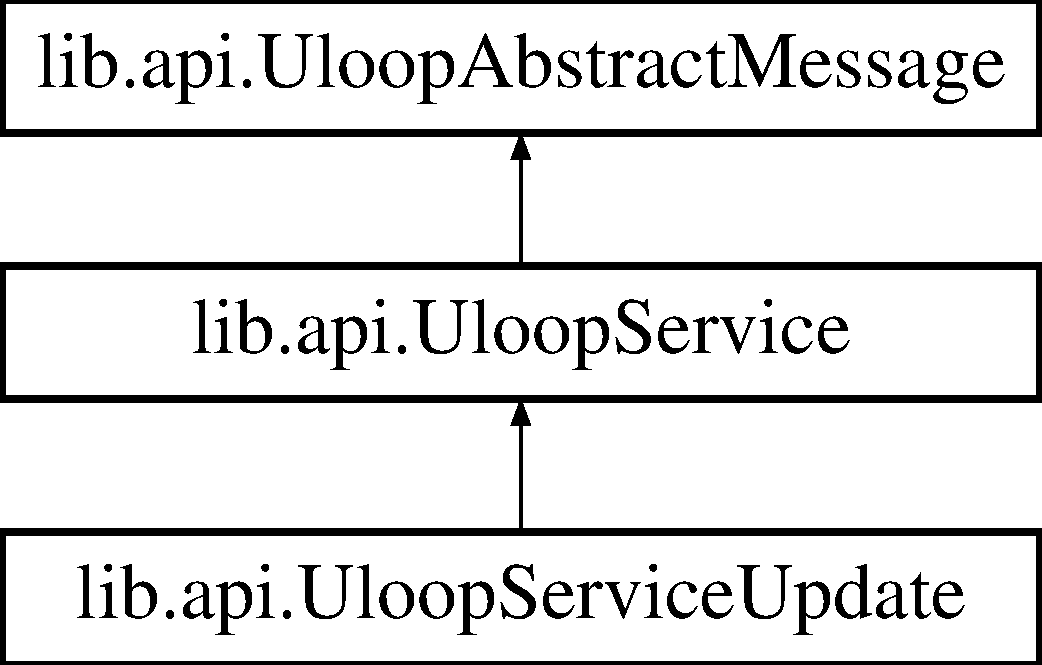
\includegraphics[height=3.000000cm]{classlib_1_1api_1_1UloopServiceUpdate}
\end{center}
\end{figure}
\subsection*{Public Member Functions}
\begin{DoxyCompactItemize}
\item 
void \hyperlink{classlib_1_1api_1_1UloopServiceUpdate_a93b43859b5331e7e9420ccfbae671c95}{set\+Crypto\+I\+D} (\hyperlink{classlib_1_1api_1_1CryptoID}{Crypto\+I\+D} cid)
\item 
\hyperlink{interfacelib_1_1api_1_1UloopAbstractMessage}{Uloop\+Abstract\+Message} \hyperlink{classlib_1_1api_1_1UloopServiceUpdate_a3bb1384447e9db3372e48356ff5a214f}{decode} (Uloop\+Message ulm)  throws Runtime\+Exception 
\item 
Builder \hyperlink{classlib_1_1api_1_1UloopServiceUpdate_a0933882171971eb0f704101ba19f36f4}{encode} ()
\item 
void \hyperlink{classlib_1_1api_1_1UloopServiceUpdate_a92cf6fa47379c50f0117838e97e7eb9d}{print} ()
\end{DoxyCompactItemize}
\subsection*{Private Attributes}
\begin{DoxyCompactItemize}
\item 
\hyperlink{classlib_1_1api_1_1CryptoID}{Crypto\+I\+D} \hyperlink{classlib_1_1api_1_1UloopServiceUpdate_aaa3de1dc764f023031f9e797fa46f3ad}{cryptoid}
\end{DoxyCompactItemize}


\subsection{Member Function Documentation}
\hypertarget{classlib_1_1api_1_1UloopServiceUpdate_a3bb1384447e9db3372e48356ff5a214f}{\index{lib\+::api\+::\+Uloop\+Service\+Update@{lib\+::api\+::\+Uloop\+Service\+Update}!decode@{decode}}
\index{decode@{decode}!lib\+::api\+::\+Uloop\+Service\+Update@{lib\+::api\+::\+Uloop\+Service\+Update}}
\subsubsection[{decode}]{\setlength{\rightskip}{0pt plus 5cm}{\bf Uloop\+Abstract\+Message} lib.\+api.\+Uloop\+Service\+Update.\+decode (
\begin{DoxyParamCaption}
\item[{Uloop\+Message}]{ulm}
\end{DoxyParamCaption}
) throws Runtime\+Exception}}\label{classlib_1_1api_1_1UloopServiceUpdate_a3bb1384447e9db3372e48356ff5a214f}


Implements \hyperlink{interfacelib_1_1api_1_1UloopAbstractMessage_a1a650d00338402b7d2a5f46575241986}{lib.\+api.\+Uloop\+Abstract\+Message}.

\hypertarget{classlib_1_1api_1_1UloopServiceUpdate_a0933882171971eb0f704101ba19f36f4}{\index{lib\+::api\+::\+Uloop\+Service\+Update@{lib\+::api\+::\+Uloop\+Service\+Update}!encode@{encode}}
\index{encode@{encode}!lib\+::api\+::\+Uloop\+Service\+Update@{lib\+::api\+::\+Uloop\+Service\+Update}}
\subsubsection[{encode}]{\setlength{\rightskip}{0pt plus 5cm}Builder lib.\+api.\+Uloop\+Service\+Update.\+encode (
\begin{DoxyParamCaption}
{}
\end{DoxyParamCaption}
)}}\label{classlib_1_1api_1_1UloopServiceUpdate_a0933882171971eb0f704101ba19f36f4}


Implements \hyperlink{interfacelib_1_1api_1_1UloopAbstractMessage_a00e05a40924dadb7ee429c811628aea3}{lib.\+api.\+Uloop\+Abstract\+Message}.

\hypertarget{classlib_1_1api_1_1UloopServiceUpdate_a92cf6fa47379c50f0117838e97e7eb9d}{\index{lib\+::api\+::\+Uloop\+Service\+Update@{lib\+::api\+::\+Uloop\+Service\+Update}!print@{print}}
\index{print@{print}!lib\+::api\+::\+Uloop\+Service\+Update@{lib\+::api\+::\+Uloop\+Service\+Update}}
\subsubsection[{print}]{\setlength{\rightskip}{0pt plus 5cm}void lib.\+api.\+Uloop\+Service\+Update.\+print (
\begin{DoxyParamCaption}
{}
\end{DoxyParamCaption}
)}}\label{classlib_1_1api_1_1UloopServiceUpdate_a92cf6fa47379c50f0117838e97e7eb9d}


Implements \hyperlink{interfacelib_1_1api_1_1UloopAbstractMessage_a116bcd258e6e384507888f4a2e2100a9}{lib.\+api.\+Uloop\+Abstract\+Message}.

\hypertarget{classlib_1_1api_1_1UloopServiceUpdate_a93b43859b5331e7e9420ccfbae671c95}{\index{lib\+::api\+::\+Uloop\+Service\+Update@{lib\+::api\+::\+Uloop\+Service\+Update}!set\+Crypto\+I\+D@{set\+Crypto\+I\+D}}
\index{set\+Crypto\+I\+D@{set\+Crypto\+I\+D}!lib\+::api\+::\+Uloop\+Service\+Update@{lib\+::api\+::\+Uloop\+Service\+Update}}
\subsubsection[{set\+Crypto\+I\+D}]{\setlength{\rightskip}{0pt plus 5cm}void lib.\+api.\+Uloop\+Service\+Update.\+set\+Crypto\+I\+D (
\begin{DoxyParamCaption}
\item[{{\bf Crypto\+I\+D}}]{cid}
\end{DoxyParamCaption}
)}}\label{classlib_1_1api_1_1UloopServiceUpdate_a93b43859b5331e7e9420ccfbae671c95}


\subsection{Member Data Documentation}
\hypertarget{classlib_1_1api_1_1UloopServiceUpdate_aaa3de1dc764f023031f9e797fa46f3ad}{\index{lib\+::api\+::\+Uloop\+Service\+Update@{lib\+::api\+::\+Uloop\+Service\+Update}!cryptoid@{cryptoid}}
\index{cryptoid@{cryptoid}!lib\+::api\+::\+Uloop\+Service\+Update@{lib\+::api\+::\+Uloop\+Service\+Update}}
\subsubsection[{cryptoid}]{\setlength{\rightskip}{0pt plus 5cm}{\bf Crypto\+I\+D} lib.\+api.\+Uloop\+Service\+Update.\+cryptoid\hspace{0.3cm}{\ttfamily [private]}}}\label{classlib_1_1api_1_1UloopServiceUpdate_aaa3de1dc764f023031f9e797fa46f3ad}


The documentation for this class was generated from the following file\+:\begin{DoxyCompactItemize}
\item 
src/lib/api/\hyperlink{UloopServiceUpdate_8java}{Uloop\+Service\+Update.\+java}\end{DoxyCompactItemize}

\hypertarget{interfaceeu_1_1uloop_1_1mobilitytracker_1_1WifiChangeListener}{\section{eu.\+uloop.\+mobilitytracker.\+Wifi\+Change\+Listener Interface Reference}
\label{interfaceeu_1_1uloop_1_1mobilitytracker_1_1WifiChangeListener}\index{eu.\+uloop.\+mobilitytracker.\+Wifi\+Change\+Listener@{eu.\+uloop.\+mobilitytracker.\+Wifi\+Change\+Listener}}
}


Inherited by eu.\+uloop.\+mobilitytracker.\+M\+Tracker\+Service.\+M\+Tracker\+Service\+Wifi\+Listener.

\subsection*{Public Member Functions}
\begin{DoxyCompactItemize}
\item 
void \hyperlink{interfaceeu_1_1uloop_1_1mobilitytracker_1_1WifiChangeListener_adaaef9d32d4cb835b49b5d3c0bf2aebe}{on\+Wifi\+State\+Disabled} (boolean valid, String bssid, String ssid, long visit\+Id, long connection\+Start, long connection\+End)
\item 
void \hyperlink{interfaceeu_1_1uloop_1_1mobilitytracker_1_1WifiChangeListener_af05047c30f56bcd75c08b703faf3cb18}{on\+Wifi\+State\+Enabled} ()
\item 
void \hyperlink{interfaceeu_1_1uloop_1_1mobilitytracker_1_1WifiChangeListener_a0e93d004d3c09bf2622fad80f9f85fb6}{on\+Wifi\+Connection\+Down} (boolean valid, String bssid, String ssid, long visit\+Id, long connection\+Start, long connection\+End)
\item 
long \hyperlink{interfaceeu_1_1uloop_1_1mobilitytracker_1_1WifiChangeListener_a6a0aacf2d36131d7a49f29bf56e4b3e2}{on\+Wifi\+Connection\+Up} (String bssid, String ssid, List$<$ Scan\+Result $>$ last\+Scan\+Results)
\item 
void \hyperlink{interfaceeu_1_1uloop_1_1mobilitytracker_1_1WifiChangeListener_aa7914e455b236cb3187024011b7660a2}{on\+Wifi\+Available\+Networks\+Change} (String bssid, List$<$ Scan\+Result $>$ results)
\end{DoxyCompactItemize}


\subsection{Member Function Documentation}
\hypertarget{interfaceeu_1_1uloop_1_1mobilitytracker_1_1WifiChangeListener_aa7914e455b236cb3187024011b7660a2}{\index{eu\+::uloop\+::mobilitytracker\+::\+Wifi\+Change\+Listener@{eu\+::uloop\+::mobilitytracker\+::\+Wifi\+Change\+Listener}!on\+Wifi\+Available\+Networks\+Change@{on\+Wifi\+Available\+Networks\+Change}}
\index{on\+Wifi\+Available\+Networks\+Change@{on\+Wifi\+Available\+Networks\+Change}!eu\+::uloop\+::mobilitytracker\+::\+Wifi\+Change\+Listener@{eu\+::uloop\+::mobilitytracker\+::\+Wifi\+Change\+Listener}}
\subsubsection[{on\+Wifi\+Available\+Networks\+Change}]{\setlength{\rightskip}{0pt plus 5cm}void eu.\+uloop.\+mobilitytracker.\+Wifi\+Change\+Listener.\+on\+Wifi\+Available\+Networks\+Change (
\begin{DoxyParamCaption}
\item[{String}]{bssid, }
\item[{List$<$ Scan\+Result $>$}]{results}
\end{DoxyParamCaption}
)}}\label{interfaceeu_1_1uloop_1_1mobilitytracker_1_1WifiChangeListener_aa7914e455b236cb3187024011b7660a2}
\hypertarget{interfaceeu_1_1uloop_1_1mobilitytracker_1_1WifiChangeListener_a0e93d004d3c09bf2622fad80f9f85fb6}{\index{eu\+::uloop\+::mobilitytracker\+::\+Wifi\+Change\+Listener@{eu\+::uloop\+::mobilitytracker\+::\+Wifi\+Change\+Listener}!on\+Wifi\+Connection\+Down@{on\+Wifi\+Connection\+Down}}
\index{on\+Wifi\+Connection\+Down@{on\+Wifi\+Connection\+Down}!eu\+::uloop\+::mobilitytracker\+::\+Wifi\+Change\+Listener@{eu\+::uloop\+::mobilitytracker\+::\+Wifi\+Change\+Listener}}
\subsubsection[{on\+Wifi\+Connection\+Down}]{\setlength{\rightskip}{0pt plus 5cm}void eu.\+uloop.\+mobilitytracker.\+Wifi\+Change\+Listener.\+on\+Wifi\+Connection\+Down (
\begin{DoxyParamCaption}
\item[{boolean}]{valid, }
\item[{String}]{bssid, }
\item[{String}]{ssid, }
\item[{long}]{visit\+Id, }
\item[{long}]{connection\+Start, }
\item[{long}]{connection\+End}
\end{DoxyParamCaption}
)}}\label{interfaceeu_1_1uloop_1_1mobilitytracker_1_1WifiChangeListener_a0e93d004d3c09bf2622fad80f9f85fb6}
\hypertarget{interfaceeu_1_1uloop_1_1mobilitytracker_1_1WifiChangeListener_a6a0aacf2d36131d7a49f29bf56e4b3e2}{\index{eu\+::uloop\+::mobilitytracker\+::\+Wifi\+Change\+Listener@{eu\+::uloop\+::mobilitytracker\+::\+Wifi\+Change\+Listener}!on\+Wifi\+Connection\+Up@{on\+Wifi\+Connection\+Up}}
\index{on\+Wifi\+Connection\+Up@{on\+Wifi\+Connection\+Up}!eu\+::uloop\+::mobilitytracker\+::\+Wifi\+Change\+Listener@{eu\+::uloop\+::mobilitytracker\+::\+Wifi\+Change\+Listener}}
\subsubsection[{on\+Wifi\+Connection\+Up}]{\setlength{\rightskip}{0pt plus 5cm}long eu.\+uloop.\+mobilitytracker.\+Wifi\+Change\+Listener.\+on\+Wifi\+Connection\+Up (
\begin{DoxyParamCaption}
\item[{String}]{bssid, }
\item[{String}]{ssid, }
\item[{List$<$ Scan\+Result $>$}]{last\+Scan\+Results}
\end{DoxyParamCaption}
)}}\label{interfaceeu_1_1uloop_1_1mobilitytracker_1_1WifiChangeListener_a6a0aacf2d36131d7a49f29bf56e4b3e2}
\hypertarget{interfaceeu_1_1uloop_1_1mobilitytracker_1_1WifiChangeListener_adaaef9d32d4cb835b49b5d3c0bf2aebe}{\index{eu\+::uloop\+::mobilitytracker\+::\+Wifi\+Change\+Listener@{eu\+::uloop\+::mobilitytracker\+::\+Wifi\+Change\+Listener}!on\+Wifi\+State\+Disabled@{on\+Wifi\+State\+Disabled}}
\index{on\+Wifi\+State\+Disabled@{on\+Wifi\+State\+Disabled}!eu\+::uloop\+::mobilitytracker\+::\+Wifi\+Change\+Listener@{eu\+::uloop\+::mobilitytracker\+::\+Wifi\+Change\+Listener}}
\subsubsection[{on\+Wifi\+State\+Disabled}]{\setlength{\rightskip}{0pt plus 5cm}void eu.\+uloop.\+mobilitytracker.\+Wifi\+Change\+Listener.\+on\+Wifi\+State\+Disabled (
\begin{DoxyParamCaption}
\item[{boolean}]{valid, }
\item[{String}]{bssid, }
\item[{String}]{ssid, }
\item[{long}]{visit\+Id, }
\item[{long}]{connection\+Start, }
\item[{long}]{connection\+End}
\end{DoxyParamCaption}
)}}\label{interfaceeu_1_1uloop_1_1mobilitytracker_1_1WifiChangeListener_adaaef9d32d4cb835b49b5d3c0bf2aebe}
\hypertarget{interfaceeu_1_1uloop_1_1mobilitytracker_1_1WifiChangeListener_af05047c30f56bcd75c08b703faf3cb18}{\index{eu\+::uloop\+::mobilitytracker\+::\+Wifi\+Change\+Listener@{eu\+::uloop\+::mobilitytracker\+::\+Wifi\+Change\+Listener}!on\+Wifi\+State\+Enabled@{on\+Wifi\+State\+Enabled}}
\index{on\+Wifi\+State\+Enabled@{on\+Wifi\+State\+Enabled}!eu\+::uloop\+::mobilitytracker\+::\+Wifi\+Change\+Listener@{eu\+::uloop\+::mobilitytracker\+::\+Wifi\+Change\+Listener}}
\subsubsection[{on\+Wifi\+State\+Enabled}]{\setlength{\rightskip}{0pt plus 5cm}void eu.\+uloop.\+mobilitytracker.\+Wifi\+Change\+Listener.\+on\+Wifi\+State\+Enabled (
\begin{DoxyParamCaption}
{}
\end{DoxyParamCaption}
)}}\label{interfaceeu_1_1uloop_1_1mobilitytracker_1_1WifiChangeListener_af05047c30f56bcd75c08b703faf3cb18}


The documentation for this interface was generated from the following file\+:\begin{DoxyCompactItemize}
\item 
src/eu/uloop/mobilitytracker/\hyperlink{WifiChangeListener_8java}{Wifi\+Change\+Listener.\+java}\end{DoxyCompactItemize}

\chapter{File Documentation}
\hypertarget{BuildConfig_8java}{\section{gen/eu/uloop/mobilitytracker/\+Build\+Config.java File Reference}
\label{BuildConfig_8java}\index{gen/eu/uloop/mobilitytracker/\+Build\+Config.\+java@{gen/eu/uloop/mobilitytracker/\+Build\+Config.\+java}}
}
\subsection*{Classes}
\begin{DoxyCompactItemize}
\item 
class \hyperlink{classeu_1_1uloop_1_1mobilitytracker_1_1BuildConfig}{eu.\+uloop.\+mobilitytracker.\+Build\+Config}
\end{DoxyCompactItemize}
\subsection*{Packages}
\begin{DoxyCompactItemize}
\item 
package \hyperlink{namespaceeu_1_1uloop_1_1mobilitytracker}{eu.\+uloop.\+mobilitytracker}
\end{DoxyCompactItemize}

\hypertarget{R_8java}{\section{gen/eu/uloop/mobilitytracker/\+R.java File Reference}
\label{R_8java}\index{gen/eu/uloop/mobilitytracker/\+R.\+java@{gen/eu/uloop/mobilitytracker/\+R.\+java}}
}
\subsection*{Classes}
\begin{DoxyCompactItemize}
\item 
class \hyperlink{classeu_1_1uloop_1_1mobilitytracker_1_1R}{eu.\+uloop.\+mobilitytracker.\+R}
\item 
class {\bfseries eu.\+uloop.\+mobilitytracker.\+R.\+attr}
\item 
class {\bfseries eu.\+uloop.\+mobilitytracker.\+R.\+dimen}
\item 
class {\bfseries eu.\+uloop.\+mobilitytracker.\+R.\+drawable}
\item 
class {\bfseries eu.\+uloop.\+mobilitytracker.\+R.\+id}
\item 
class {\bfseries eu.\+uloop.\+mobilitytracker.\+R.\+layout}
\item 
class {\bfseries eu.\+uloop.\+mobilitytracker.\+R.\+menu}
\item 
class {\bfseries eu.\+uloop.\+mobilitytracker.\+R.\+string}
\item 
class {\bfseries eu.\+uloop.\+mobilitytracker.\+R.\+style}
\end{DoxyCompactItemize}
\subsection*{Packages}
\begin{DoxyCompactItemize}
\item 
package \hyperlink{namespaceeu_1_1uloop_1_1mobilitytracker}{eu.\+uloop.\+mobilitytracker}
\end{DoxyCompactItemize}

\hypertarget{UloopMessages_8java}{\section{src/eu/uloop/messages/\+Uloop\+Messages.java File Reference}
\label{UloopMessages_8java}\index{src/eu/uloop/messages/\+Uloop\+Messages.\+java@{src/eu/uloop/messages/\+Uloop\+Messages.\+java}}
}
\subsection*{Classes}
\begin{DoxyCompactItemize}
\item 
class \hyperlink{classeu_1_1uloop_1_1messages_1_1UloopMessages}{eu.\+uloop.\+messages.\+Uloop\+Messages}
\item 
enum \hyperlink{enumeu_1_1uloop_1_1messages_1_1UloopMessages_1_1MessageType}{eu.\+uloop.\+messages.\+Uloop\+Messages.\+Message\+Type}
\item 
enum \hyperlink{enumeu_1_1uloop_1_1messages_1_1UloopMessages_1_1UloopMessageType}{eu.\+uloop.\+messages.\+Uloop\+Messages.\+Uloop\+Message\+Type}
\item 
interface \hyperlink{interfaceeu_1_1uloop_1_1messages_1_1UloopMessages_1_1UloopHeaderMessageOrBuilder}{eu.\+uloop.\+messages.\+Uloop\+Messages.\+Uloop\+Header\+Message\+Or\+Builder}
\item 
class {\bfseries eu.\+uloop.\+messages.\+Uloop\+Messages.\+Uloop\+Header\+Message}
\item 
class {\bfseries eu.\+uloop.\+messages.\+Uloop\+Messages.\+Uloop\+Header\+Message.\+Builder}
\item 
interface \hyperlink{interfaceeu_1_1uloop_1_1messages_1_1UloopMessages_1_1UloopMessageOrBuilder}{eu.\+uloop.\+messages.\+Uloop\+Messages.\+Uloop\+Message\+Or\+Builder}
\item 
class {\bfseries eu.\+uloop.\+messages.\+Uloop\+Messages.\+Uloop\+Message}
\item 
class {\bfseries eu.\+uloop.\+messages.\+Uloop\+Messages.\+Uloop\+Message.\+Builder}
\item 
interface \hyperlink{interfaceeu_1_1uloop_1_1messages_1_1UloopMessages_1_1TrustMessageOrBuilder}{eu.\+uloop.\+messages.\+Uloop\+Messages.\+Trust\+Message\+Or\+Builder}
\item 
class {\bfseries eu.\+uloop.\+messages.\+Uloop\+Messages.\+Trust\+Message}
\item 
class {\bfseries eu.\+uloop.\+messages.\+Uloop\+Messages.\+Trust\+Message.\+Builder}
\item 
interface \hyperlink{interfaceeu_1_1uloop_1_1messages_1_1UloopMessages_1_1TrustInformationRequestOrBuilder}{eu.\+uloop.\+messages.\+Uloop\+Messages.\+Trust\+Information\+Request\+Or\+Builder}
\item 
class {\bfseries eu.\+uloop.\+messages.\+Uloop\+Messages.\+Trust\+Information\+Request}
\item 
class {\bfseries eu.\+uloop.\+messages.\+Uloop\+Messages.\+Trust\+Information\+Request.\+Builder}
\item 
interface \hyperlink{interfaceeu_1_1uloop_1_1messages_1_1UloopMessages_1_1TrustInformationReplyOrBuilder}{eu.\+uloop.\+messages.\+Uloop\+Messages.\+Trust\+Information\+Reply\+Or\+Builder}
\item 
class {\bfseries eu.\+uloop.\+messages.\+Uloop\+Messages.\+Trust\+Information\+Reply}
\item 
class {\bfseries eu.\+uloop.\+messages.\+Uloop\+Messages.\+Trust\+Information\+Reply.\+Builder}
\item 
interface \hyperlink{interfaceeu_1_1uloop_1_1messages_1_1UloopMessages_1_1ResourceMessageOrBuilder}{eu.\+uloop.\+messages.\+Uloop\+Messages.\+Resource\+Message\+Or\+Builder}
\item 
class {\bfseries eu.\+uloop.\+messages.\+Uloop\+Messages.\+Resource\+Message}
\item 
class {\bfseries eu.\+uloop.\+messages.\+Uloop\+Messages.\+Resource\+Message.\+Builder}
\item 
interface \hyperlink{interfaceeu_1_1uloop_1_1messages_1_1UloopMessages_1_1EnoughResourcesMessageRequestOrBuilder}{eu.\+uloop.\+messages.\+Uloop\+Messages.\+Enough\+Resources\+Message\+Request\+Or\+Builder}
\item 
class {\bfseries eu.\+uloop.\+messages.\+Uloop\+Messages.\+Enough\+Resources\+Message\+Request}
\item 
class {\bfseries eu.\+uloop.\+messages.\+Uloop\+Messages.\+Enough\+Resources\+Message\+Request.\+Builder}
\item 
interface \hyperlink{interfaceeu_1_1uloop_1_1messages_1_1UloopMessages_1_1EnoughResourcesMessageReplyOrBuilder}{eu.\+uloop.\+messages.\+Uloop\+Messages.\+Enough\+Resources\+Message\+Reply\+Or\+Builder}
\item 
class {\bfseries eu.\+uloop.\+messages.\+Uloop\+Messages.\+Enough\+Resources\+Message\+Reply}
\item 
class {\bfseries eu.\+uloop.\+messages.\+Uloop\+Messages.\+Enough\+Resources\+Message\+Reply.\+Builder}
\item 
interface \hyperlink{interfaceeu_1_1uloop_1_1messages_1_1UloopMessages_1_1NetworkStatusMessageOrBuilder}{eu.\+uloop.\+messages.\+Uloop\+Messages.\+Network\+Status\+Message\+Or\+Builder}
\item 
class {\bfseries eu.\+uloop.\+messages.\+Uloop\+Messages.\+Network\+Status\+Message}
\item 
class {\bfseries eu.\+uloop.\+messages.\+Uloop\+Messages.\+Network\+Status\+Message.\+Builder}
\item 
interface \hyperlink{interfaceeu_1_1uloop_1_1messages_1_1UloopMessages_1_1NetworkStatusMessageReplyOrBuilder}{eu.\+uloop.\+messages.\+Uloop\+Messages.\+Network\+Status\+Message\+Reply\+Or\+Builder}
\item 
class {\bfseries eu.\+uloop.\+messages.\+Uloop\+Messages.\+Network\+Status\+Message\+Reply}
\item 
class {\bfseries eu.\+uloop.\+messages.\+Uloop\+Messages.\+Network\+Status\+Message\+Reply.\+Builder}
\item 
interface \hyperlink{interfaceeu_1_1uloop_1_1messages_1_1UloopMessages_1_1NewUserDetailsMessageOrBuilder}{eu.\+uloop.\+messages.\+Uloop\+Messages.\+New\+User\+Details\+Message\+Or\+Builder}
\item 
class {\bfseries eu.\+uloop.\+messages.\+Uloop\+Messages.\+New\+User\+Details\+Message}
\item 
class {\bfseries eu.\+uloop.\+messages.\+Uloop\+Messages.\+New\+User\+Details\+Message.\+Builder}
\item 
interface \hyperlink{interfaceeu_1_1uloop_1_1messages_1_1UloopMessages_1_1EnoughResourcesCACReplyOrBuilder}{eu.\+uloop.\+messages.\+Uloop\+Messages.\+Enough\+Resources\+C\+A\+C\+Reply\+Or\+Builder}
\item 
class {\bfseries eu.\+uloop.\+messages.\+Uloop\+Messages.\+Enough\+Resources\+C\+A\+C\+Reply}
\item 
class {\bfseries eu.\+uloop.\+messages.\+Uloop\+Messages.\+Enough\+Resources\+C\+A\+C\+Reply.\+Builder}
\item 
interface \hyperlink{interfaceeu_1_1uloop_1_1messages_1_1UloopMessages_1_1QoSTupleOrBuilder}{eu.\+uloop.\+messages.\+Uloop\+Messages.\+Qo\+S\+Tuple\+Or\+Builder}
\item 
class {\bfseries eu.\+uloop.\+messages.\+Uloop\+Messages.\+Qo\+S\+Tuple}
\item 
class {\bfseries eu.\+uloop.\+messages.\+Uloop\+Messages.\+Qo\+S\+Tuple.\+Builder}
\item 
interface \hyperlink{interfaceeu_1_1uloop_1_1messages_1_1UloopMessages_1_1QosRequestOrBuilder}{eu.\+uloop.\+messages.\+Uloop\+Messages.\+Qos\+Request\+Or\+Builder}
\item 
class {\bfseries eu.\+uloop.\+messages.\+Uloop\+Messages.\+Qos\+Request}
\item 
class {\bfseries eu.\+uloop.\+messages.\+Uloop\+Messages.\+Qos\+Request.\+Builder}
\item 
interface \hyperlink{interfaceeu_1_1uloop_1_1messages_1_1UloopMessages_1_1QoSMessageOrBuilder}{eu.\+uloop.\+messages.\+Uloop\+Messages.\+Qo\+S\+Message\+Or\+Builder}
\item 
class {\bfseries eu.\+uloop.\+messages.\+Uloop\+Messages.\+Qo\+S\+Message}
\item 
class {\bfseries eu.\+uloop.\+messages.\+Uloop\+Messages.\+Qo\+S\+Message.\+Builder}
\item 
interface \hyperlink{interfaceeu_1_1uloop_1_1messages_1_1UloopMessages_1_1ServiceMessageOrBuilder}{eu.\+uloop.\+messages.\+Uloop\+Messages.\+Service\+Message\+Or\+Builder}
\item 
class {\bfseries eu.\+uloop.\+messages.\+Uloop\+Messages.\+Service\+Message}
\item 
class {\bfseries eu.\+uloop.\+messages.\+Uloop\+Messages.\+Service\+Message.\+Builder}
\item 
interface \hyperlink{interfaceeu_1_1uloop_1_1messages_1_1UloopMessages_1_1ServiceRequestOrBuilder}{eu.\+uloop.\+messages.\+Uloop\+Messages.\+Service\+Request\+Or\+Builder}
\item 
class {\bfseries eu.\+uloop.\+messages.\+Uloop\+Messages.\+Service\+Request}
\item 
class {\bfseries eu.\+uloop.\+messages.\+Uloop\+Messages.\+Service\+Request.\+Builder}
\item 
interface \hyperlink{interfaceeu_1_1uloop_1_1messages_1_1UloopMessages_1_1ServiceReplyOrBuilder}{eu.\+uloop.\+messages.\+Uloop\+Messages.\+Service\+Reply\+Or\+Builder}
\item 
class {\bfseries eu.\+uloop.\+messages.\+Uloop\+Messages.\+Service\+Reply}
\item 
class {\bfseries eu.\+uloop.\+messages.\+Uloop\+Messages.\+Service\+Reply.\+Builder}
\item 
interface \hyperlink{interfaceeu_1_1uloop_1_1messages_1_1UloopMessages_1_1ServiceUpdateOrBuilder}{eu.\+uloop.\+messages.\+Uloop\+Messages.\+Service\+Update\+Or\+Builder}
\item 
class {\bfseries eu.\+uloop.\+messages.\+Uloop\+Messages.\+Service\+Update}
\item 
class {\bfseries eu.\+uloop.\+messages.\+Uloop\+Messages.\+Service\+Update.\+Builder}
\item 
interface \hyperlink{interfaceeu_1_1uloop_1_1messages_1_1UloopMessages_1_1MTrackerPredictedMoveOrBuilder}{eu.\+uloop.\+messages.\+Uloop\+Messages.\+M\+Tracker\+Predicted\+Move\+Or\+Builder}
\item 
class {\bfseries eu.\+uloop.\+messages.\+Uloop\+Messages.\+M\+Tracker\+Predicted\+Move}
\item 
class {\bfseries eu.\+uloop.\+messages.\+Uloop\+Messages.\+M\+Tracker\+Predicted\+Move.\+Builder}
\item 
interface \hyperlink{interfaceeu_1_1uloop_1_1messages_1_1UloopMessages_1_1MTrackerMessageOrBuilder}{eu.\+uloop.\+messages.\+Uloop\+Messages.\+M\+Tracker\+Message\+Or\+Builder}
\item 
class {\bfseries eu.\+uloop.\+messages.\+Uloop\+Messages.\+M\+Tracker\+Message}
\item 
class {\bfseries eu.\+uloop.\+messages.\+Uloop\+Messages.\+M\+Tracker\+Message.\+Builder}
\end{DoxyCompactItemize}
\subsection*{Packages}
\begin{DoxyCompactItemize}
\item 
package \hyperlink{namespaceeu_1_1uloop_1_1messages}{eu.\+uloop.\+messages}
\end{DoxyCompactItemize}

\hypertarget{DataBaseChangeListener_8java}{\section{src/eu/uloop/mobilitytracker/\+Data\+Base\+Change\+Listener.java File Reference}
\label{DataBaseChangeListener_8java}\index{src/eu/uloop/mobilitytracker/\+Data\+Base\+Change\+Listener.\+java@{src/eu/uloop/mobilitytracker/\+Data\+Base\+Change\+Listener.\+java}}
}
\subsection*{Classes}
\begin{DoxyCompactItemize}
\item 
interface \hyperlink{interfaceeu_1_1uloop_1_1mobilitytracker_1_1DataBaseChangeListener}{eu.\+uloop.\+mobilitytracker.\+Data\+Base\+Change\+Listener}
\end{DoxyCompactItemize}
\subsection*{Packages}
\begin{DoxyCompactItemize}
\item 
package \hyperlink{namespaceeu_1_1uloop_1_1mobilitytracker}{eu.\+uloop.\+mobilitytracker}
\end{DoxyCompactItemize}

\hypertarget{DetailsActivity_8java}{\section{src/eu/uloop/mobilitytracker/\+Details\+Activity.java File Reference}
\label{DetailsActivity_8java}\index{src/eu/uloop/mobilitytracker/\+Details\+Activity.\+java@{src/eu/uloop/mobilitytracker/\+Details\+Activity.\+java}}
}
\subsection*{Classes}
\begin{DoxyCompactItemize}
\item 
class \hyperlink{classeu_1_1uloop_1_1mobilitytracker_1_1DetailsActivity}{eu.\+uloop.\+mobilitytracker.\+Details\+Activity}
\end{DoxyCompactItemize}
\subsection*{Packages}
\begin{DoxyCompactItemize}
\item 
package \hyperlink{namespaceeu_1_1uloop_1_1mobilitytracker}{eu.\+uloop.\+mobilitytracker}
\end{DoxyCompactItemize}

\hypertarget{MTrackerAP_8java}{\section{src/eu/uloop/mobilitytracker/\+M\+Tracker\+A\+P.java File Reference}
\label{MTrackerAP_8java}\index{src/eu/uloop/mobilitytracker/\+M\+Tracker\+A\+P.\+java@{src/eu/uloop/mobilitytracker/\+M\+Tracker\+A\+P.\+java}}
}
\subsection*{Classes}
\begin{DoxyCompactItemize}
\item 
class \hyperlink{classeu_1_1uloop_1_1mobilitytracker_1_1MTrackerAP}{eu.\+uloop.\+mobilitytracker.\+M\+Tracker\+A\+P}
\end{DoxyCompactItemize}
\subsection*{Packages}
\begin{DoxyCompactItemize}
\item 
package \hyperlink{namespaceeu_1_1uloop_1_1mobilitytracker}{eu.\+uloop.\+mobilitytracker}
\end{DoxyCompactItemize}

\hypertarget{MTrackerApplication_8java}{\section{src/eu/uloop/mobilitytracker/\+M\+Tracker\+Application.java File Reference}
\label{MTrackerApplication_8java}\index{src/eu/uloop/mobilitytracker/\+M\+Tracker\+Application.\+java@{src/eu/uloop/mobilitytracker/\+M\+Tracker\+Application.\+java}}
}
\subsection*{Classes}
\begin{DoxyCompactItemize}
\item 
class \hyperlink{classeu_1_1uloop_1_1mobilitytracker_1_1MTrackerApplication}{eu.\+uloop.\+mobilitytracker.\+M\+Tracker\+Application}
\end{DoxyCompactItemize}
\subsection*{Packages}
\begin{DoxyCompactItemize}
\item 
package \hyperlink{namespaceeu_1_1uloop_1_1mobilitytracker}{eu.\+uloop.\+mobilitytracker}
\end{DoxyCompactItemize}

\hypertarget{MTrackerDataSource_8java}{\section{src/eu/uloop/mobilitytracker/\+M\+Tracker\+Data\+Source.java File Reference}
\label{MTrackerDataSource_8java}\index{src/eu/uloop/mobilitytracker/\+M\+Tracker\+Data\+Source.\+java@{src/eu/uloop/mobilitytracker/\+M\+Tracker\+Data\+Source.\+java}}
}
\subsection*{Classes}
\begin{DoxyCompactItemize}
\item 
class \hyperlink{classeu_1_1uloop_1_1mobilitytracker_1_1MTrackerDataSource}{eu.\+uloop.\+mobilitytracker.\+M\+Tracker\+Data\+Source}
\end{DoxyCompactItemize}
\subsection*{Packages}
\begin{DoxyCompactItemize}
\item 
package \hyperlink{namespaceeu_1_1uloop_1_1mobilitytracker}{eu.\+uloop.\+mobilitytracker}
\end{DoxyCompactItemize}

\hypertarget{MTrackerService_8java}{\section{src/eu/uloop/mobilitytracker/\+M\+Tracker\+Service.java File Reference}
\label{MTrackerService_8java}\index{src/eu/uloop/mobilitytracker/\+M\+Tracker\+Service.\+java@{src/eu/uloop/mobilitytracker/\+M\+Tracker\+Service.\+java}}
}
\subsection*{Classes}
\begin{DoxyCompactItemize}
\item 
class \hyperlink{classeu_1_1uloop_1_1mobilitytracker_1_1MTrackerService}{eu.\+uloop.\+mobilitytracker.\+M\+Tracker\+Service}
\item 
class \hyperlink{classeu_1_1uloop_1_1mobilitytracker_1_1MTrackerService_1_1LocalBinder}{eu.\+uloop.\+mobilitytracker.\+M\+Tracker\+Service.\+Local\+Binder}
\item 
class {\bfseries eu.\+uloop.\+mobilitytracker.\+M\+Tracker\+Service.\+M\+Tracker\+Service\+Wifi\+Listener}
\item 
class \hyperlink{classeu_1_1uloop_1_1mobilitytracker_1_1MTrackerService_1_1SendInformationWithGatewayTask}{eu.\+uloop.\+mobilitytracker.\+M\+Tracker\+Service.\+Send\+Information\+With\+Gateway\+Task}
\end{DoxyCompactItemize}
\subsection*{Packages}
\begin{DoxyCompactItemize}
\item 
package \hyperlink{namespaceeu_1_1uloop_1_1mobilitytracker}{eu.\+uloop.\+mobilitytracker}
\end{DoxyCompactItemize}

\hypertarget{MTrackerSQLiteHelper_8java}{\section{src/eu/uloop/mobilitytracker/\+M\+Tracker\+S\+Q\+Lite\+Helper.java File Reference}
\label{MTrackerSQLiteHelper_8java}\index{src/eu/uloop/mobilitytracker/\+M\+Tracker\+S\+Q\+Lite\+Helper.\+java@{src/eu/uloop/mobilitytracker/\+M\+Tracker\+S\+Q\+Lite\+Helper.\+java}}
}
\subsection*{Classes}
\begin{DoxyCompactItemize}
\item 
class \hyperlink{classeu_1_1uloop_1_1mobilitytracker_1_1MTrackerSQLiteHelper}{eu.\+uloop.\+mobilitytracker.\+M\+Tracker\+S\+Q\+Lite\+Helper}
\end{DoxyCompactItemize}
\subsection*{Packages}
\begin{DoxyCompactItemize}
\item 
package \hyperlink{namespaceeu_1_1uloop_1_1mobilitytracker}{eu.\+uloop.\+mobilitytracker}
\end{DoxyCompactItemize}

\hypertarget{MTrackerVisit_8java}{\section{src/eu/uloop/mobilitytracker/\+M\+Tracker\+Visit.java File Reference}
\label{MTrackerVisit_8java}\index{src/eu/uloop/mobilitytracker/\+M\+Tracker\+Visit.\+java@{src/eu/uloop/mobilitytracker/\+M\+Tracker\+Visit.\+java}}
}
\subsection*{Classes}
\begin{DoxyCompactItemize}
\item 
class \hyperlink{classeu_1_1uloop_1_1mobilitytracker_1_1MTrackerVisit}{eu.\+uloop.\+mobilitytracker.\+M\+Tracker\+Visit}
\end{DoxyCompactItemize}
\subsection*{Packages}
\begin{DoxyCompactItemize}
\item 
package \hyperlink{namespaceeu_1_1uloop_1_1mobilitytracker}{eu.\+uloop.\+mobilitytracker}
\end{DoxyCompactItemize}

\hypertarget{MTrackerWifiManager_8java}{\section{src/eu/uloop/mobilitytracker/\+M\+Tracker\+Wifi\+Manager.java File Reference}
\label{MTrackerWifiManager_8java}\index{src/eu/uloop/mobilitytracker/\+M\+Tracker\+Wifi\+Manager.\+java@{src/eu/uloop/mobilitytracker/\+M\+Tracker\+Wifi\+Manager.\+java}}
}
\subsection*{Classes}
\begin{DoxyCompactItemize}
\item 
class \hyperlink{classeu_1_1uloop_1_1mobilitytracker_1_1MTrackerWifiManager}{eu.\+uloop.\+mobilitytracker.\+M\+Tracker\+Wifi\+Manager}
\item 
class {\bfseries eu.\+uloop.\+mobilitytracker.\+M\+Tracker\+Wifi\+Manager.\+Wifi\+State\+Change}
\item 
class {\bfseries eu.\+uloop.\+mobilitytracker.\+M\+Tracker\+Wifi\+Manager.\+Wifi\+Connection\+Change}
\item 
class {\bfseries eu.\+uloop.\+mobilitytracker.\+M\+Tracker\+Wifi\+Manager.\+Wifi\+Available\+Networks\+Change}
\end{DoxyCompactItemize}
\subsection*{Packages}
\begin{DoxyCompactItemize}
\item 
package \hyperlink{namespaceeu_1_1uloop_1_1mobilitytracker}{eu.\+uloop.\+mobilitytracker}
\end{DoxyCompactItemize}

\hypertarget{WifiChangeListener_8java}{\section{src/eu/uloop/mobilitytracker/\+Wifi\+Change\+Listener.java File Reference}
\label{WifiChangeListener_8java}\index{src/eu/uloop/mobilitytracker/\+Wifi\+Change\+Listener.\+java@{src/eu/uloop/mobilitytracker/\+Wifi\+Change\+Listener.\+java}}
}
\subsection*{Classes}
\begin{DoxyCompactItemize}
\item 
interface \hyperlink{interfaceeu_1_1uloop_1_1mobilitytracker_1_1WifiChangeListener}{eu.\+uloop.\+mobilitytracker.\+Wifi\+Change\+Listener}
\end{DoxyCompactItemize}
\subsection*{Packages}
\begin{DoxyCompactItemize}
\item 
package \hyperlink{namespaceeu_1_1uloop_1_1mobilitytracker}{eu.\+uloop.\+mobilitytracker}
\end{DoxyCompactItemize}

\hypertarget{CryptoID_8java}{\section{src/lib/api/\+Crypto\+I\+D.java File Reference}
\label{CryptoID_8java}\index{src/lib/api/\+Crypto\+I\+D.\+java@{src/lib/api/\+Crypto\+I\+D.\+java}}
}
\subsection*{Classes}
\begin{DoxyCompactItemize}
\item 
class \hyperlink{classlib_1_1api_1_1CryptoID}{lib.\+api.\+Crypto\+I\+D}
\end{DoxyCompactItemize}
\subsection*{Packages}
\begin{DoxyCompactItemize}
\item 
package \hyperlink{namespacelib_1_1api}{lib.\+api}
\end{DoxyCompactItemize}

\hypertarget{MessageDigest_8java}{\section{src/lib/api/\+Message\+Digest.java File Reference}
\label{MessageDigest_8java}\index{src/lib/api/\+Message\+Digest.\+java@{src/lib/api/\+Message\+Digest.\+java}}
}
\subsection*{Classes}
\begin{DoxyCompactItemize}
\item 
class \hyperlink{classlib_1_1api_1_1MessageDigest}{lib.\+api.\+Message\+Digest}
\end{DoxyCompactItemize}
\subsection*{Packages}
\begin{DoxyCompactItemize}
\item 
package \hyperlink{namespacelib_1_1api}{lib.\+api}
\end{DoxyCompactItemize}

\hypertarget{UloopAbstractMessage_8java}{\section{src/lib/api/\+Uloop\+Abstract\+Message.java File Reference}
\label{UloopAbstractMessage_8java}\index{src/lib/api/\+Uloop\+Abstract\+Message.\+java@{src/lib/api/\+Uloop\+Abstract\+Message.\+java}}
}
\subsection*{Classes}
\begin{DoxyCompactItemize}
\item 
interface \hyperlink{interfacelib_1_1api_1_1UloopAbstractMessage}{lib.\+api.\+Uloop\+Abstract\+Message}
\end{DoxyCompactItemize}
\subsection*{Packages}
\begin{DoxyCompactItemize}
\item 
package \hyperlink{namespacelib_1_1api}{lib.\+api}
\end{DoxyCompactItemize}

\hypertarget{UloopMessageAPI_8java}{\section{src/lib/api/\+Uloop\+Message\+A\+P\+I.java File Reference}
\label{UloopMessageAPI_8java}\index{src/lib/api/\+Uloop\+Message\+A\+P\+I.\+java@{src/lib/api/\+Uloop\+Message\+A\+P\+I.\+java}}
}
\subsection*{Classes}
\begin{DoxyCompactItemize}
\item 
interface \hyperlink{interfacelib_1_1api_1_1UloopMessageAPI}{lib.\+api.\+Uloop\+Message\+A\+P\+I}
\end{DoxyCompactItemize}
\subsection*{Packages}
\begin{DoxyCompactItemize}
\item 
package \hyperlink{namespacelib_1_1api}{lib.\+api}
\end{DoxyCompactItemize}

\hypertarget{UloopMessageAPIImp_8java}{\section{src/lib/api/\+Uloop\+Message\+A\+P\+I\+Imp.java File Reference}
\label{UloopMessageAPIImp_8java}\index{src/lib/api/\+Uloop\+Message\+A\+P\+I\+Imp.\+java@{src/lib/api/\+Uloop\+Message\+A\+P\+I\+Imp.\+java}}
}
\subsection*{Classes}
\begin{DoxyCompactItemize}
\item 
class \hyperlink{classlib_1_1api_1_1UloopMessageAPIImp}{lib.\+api.\+Uloop\+Message\+A\+P\+I\+Imp}
\end{DoxyCompactItemize}
\subsection*{Packages}
\begin{DoxyCompactItemize}
\item 
package \hyperlink{namespacelib_1_1api}{lib.\+api}
\end{DoxyCompactItemize}

\hypertarget{UloopMTracker_8java}{\section{src/lib/api/\+Uloop\+M\+Tracker.java File Reference}
\label{UloopMTracker_8java}\index{src/lib/api/\+Uloop\+M\+Tracker.\+java@{src/lib/api/\+Uloop\+M\+Tracker.\+java}}
}
\subsection*{Classes}
\begin{DoxyCompactItemize}
\item 
class \hyperlink{classlib_1_1api_1_1UloopMTracker}{lib.\+api.\+Uloop\+M\+Tracker}
\end{DoxyCompactItemize}
\subsection*{Packages}
\begin{DoxyCompactItemize}
\item 
package \hyperlink{namespacelib_1_1api}{lib.\+api}
\end{DoxyCompactItemize}

\hypertarget{UloopMTrackerMessage_8java}{\section{src/lib/api/\+Uloop\+M\+Tracker\+Message.java File Reference}
\label{UloopMTrackerMessage_8java}\index{src/lib/api/\+Uloop\+M\+Tracker\+Message.\+java@{src/lib/api/\+Uloop\+M\+Tracker\+Message.\+java}}
}
\subsection*{Classes}
\begin{DoxyCompactItemize}
\item 
class \hyperlink{classlib_1_1api_1_1UloopMTrackerMessage}{lib.\+api.\+Uloop\+M\+Tracker\+Message}
\item 
class \hyperlink{classlib_1_1api_1_1UloopMTrackerMessage_1_1MTrackerPredictedM}{lib.\+api.\+Uloop\+M\+Tracker\+Message.\+M\+Tracker\+Predicted\+M}
\end{DoxyCompactItemize}
\subsection*{Packages}
\begin{DoxyCompactItemize}
\item 
package \hyperlink{namespacelib_1_1api}{lib.\+api}
\end{DoxyCompactItemize}

\hypertarget{UloopService_8java}{\section{src/lib/api/\+Uloop\+Service.java File Reference}
\label{UloopService_8java}\index{src/lib/api/\+Uloop\+Service.\+java@{src/lib/api/\+Uloop\+Service.\+java}}
}
\subsection*{Classes}
\begin{DoxyCompactItemize}
\item 
class \hyperlink{classlib_1_1api_1_1UloopService}{lib.\+api.\+Uloop\+Service}
\end{DoxyCompactItemize}
\subsection*{Packages}
\begin{DoxyCompactItemize}
\item 
package \hyperlink{namespacelib_1_1api}{lib.\+api}
\end{DoxyCompactItemize}

\hypertarget{UloopServiceReply_8java}{\section{src/lib/api/\+Uloop\+Service\+Reply.java File Reference}
\label{UloopServiceReply_8java}\index{src/lib/api/\+Uloop\+Service\+Reply.\+java@{src/lib/api/\+Uloop\+Service\+Reply.\+java}}
}
\subsection*{Classes}
\begin{DoxyCompactItemize}
\item 
class \hyperlink{classlib_1_1api_1_1UloopServiceReply}{lib.\+api.\+Uloop\+Service\+Reply}
\end{DoxyCompactItemize}
\subsection*{Packages}
\begin{DoxyCompactItemize}
\item 
package \hyperlink{namespacelib_1_1api}{lib.\+api}
\end{DoxyCompactItemize}

\hypertarget{UloopServiceRequest_8java}{\section{src/lib/api/\+Uloop\+Service\+Request.java File Reference}
\label{UloopServiceRequest_8java}\index{src/lib/api/\+Uloop\+Service\+Request.\+java@{src/lib/api/\+Uloop\+Service\+Request.\+java}}
}
\subsection*{Classes}
\begin{DoxyCompactItemize}
\item 
class \hyperlink{classlib_1_1api_1_1UloopServiceRequest}{lib.\+api.\+Uloop\+Service\+Request}
\end{DoxyCompactItemize}
\subsection*{Packages}
\begin{DoxyCompactItemize}
\item 
package \hyperlink{namespacelib_1_1api}{lib.\+api}
\end{DoxyCompactItemize}

\hypertarget{UloopServiceUpdate_8java}{\section{src/lib/api/\+Uloop\+Service\+Update.java File Reference}
\label{UloopServiceUpdate_8java}\index{src/lib/api/\+Uloop\+Service\+Update.\+java@{src/lib/api/\+Uloop\+Service\+Update.\+java}}
}
\subsection*{Classes}
\begin{DoxyCompactItemize}
\item 
class \hyperlink{classlib_1_1api_1_1UloopServiceUpdate}{lib.\+api.\+Uloop\+Service\+Update}
\end{DoxyCompactItemize}
\subsection*{Packages}
\begin{DoxyCompactItemize}
\item 
package \hyperlink{namespacelib_1_1api}{lib.\+api}
\end{DoxyCompactItemize}

%--- End generated contents ---

% Index
\newpage
\phantomsection
\addcontentsline{toc}{chapter}{Index}
\printindex

\end{document}
